\documentclass[11pt,a4paper]{memoir}

\usepackage{rotating}
\usepackage{subfig}
\usepackage{amsmath}
\usepackage{rotating}
\usepackage{multirow}
\usepackage{bookman}
\usepackage{lettrine}
\usepackage{booktabs}
%\usepackage[margin=1in]{geometry}
\usepackage{natbib}
\usepackage{tikz}
    \usetikzlibrary{positioning}


\usepackage{fourier} 
\makeatletter 
\newif\iffelinenonum 
\newcommand\MyNumToName[1]{%
      \ifcase#1\relax % case 0 
      \or First\or Second\or Third% 
      \else Not implemented\fi}
      
\makechapterstyle{daleif3}{ 
  \renewcommand\chapternamenum{} 
  \renewcommand\printchaptername{} 
  \renewcommand\chapnamefont{\Large\itshape\centering} 
  \setlength\midchapskip{7pt} 
  \renewcommand\printchapternum{%
          \par\chapnamefont\decofourleft\enspace% 
          \ifanappendix \appendixname\space\thechapter% 
          \else% 
          \MyNumToName{\thechapter}\space\chaptername% 
          \fi%
          \/\enspace\decofourright} 
\renewcommand\printchapternonum{\par\felinenonumtrue} 
\renewcommand\chaptitlefont{\huge\itshape\centering} 
\renewcommand\afterchapternum{%
  \par\nobreak\vskip-5pt%
}
        
\renewcommand\afterchaptertitle{% 
  \par\vskip-2\midchapskip% 
  \rule\textwidth\normalrulethickness \felinenonumfalse 
  \nobreak\vskip\afterchapskip%
  }
} 
\makeatother 
\chapterstyle{daleif3}

\pagestyle{ruled}

\linespread{1.2}

%\includeonly{VoteChoice_Chapter/VoteChoice}

\begin{document} 

\chapter{Introduction}

\lettrine[lines = 3]{T}{he} European Union (EU) lies today at the heart of much of the legislative activities in the member states. During its 51 years of existence in  various guises, the powers and competences of the EU have steadily increased.



As the EU has gained more competences the Council has become an ever more important institution. 



As the main legislative body, every commission proposal must pass through the Council in order to become legislation. The Council occupies an uneasy position in the EU machinery. It is a Community institution, which also consists of 27 member state governments. These member states governments come together in the Council with diverse policy preferences and negotiate agreements. Since the introduction of the co-decision procedure, now the ordinary legislative procedure, in its various incarnations, the Council and the European Parliament (EP) essentially now forms a two-chamber system of governance in the EU. A lot of research has been conducted o the EP, especially with regards to voting behavior and coalition formation [REFERENCES], facilitated by the great openness of the institution. However the Council has been less open, and  


The importance of EU legislation, hence the importance of understanding the Council


The council as the most importan institution.

The EP as a co legislator

The importance of EU legislation, hence the importance of understanding the Council

How does the Council work

What we know so far

Critique

What is the purpose of this book? research question!

research design




The literature on the Council of ministers has within the last couple of years reached a level of maturity where we know have three (almost) universally accepted stylized facts.

\begin{enumerate}
\item Council decision making is structured by a wish to reach consensus.
\item There are weak cleavages that structure conflict (north-south, new-old, left-right)
\item The presidency matters
\end{enumerate}

Of these stylized facts the least tested is the claim that a norm of consensus has a strong causal effect on decision making in the Council. The common argument for the consensus norm has three key components. First actors interact with each other in an insulated environment. Secondly the population of negotiators change very slowly, so actors can build up long histories of interactions. Thirdly, this allows for the development of diffuse reciprocity. Once diffuse reciprocity is present, then the development of a consensus norm follows closely. 

The evidence for a consensus norm comes from three sources, namely case studies, council voting records and the DEU data set. The use of different kinds of data, not surprisingly, impacts the conclusions reached [WRITE MORE]. However the conceptualization of the consensus norm also differ across approaches, with the quantitative studies often employing a simple indicator for consensual voting as evidence for the consensus norm. In contrast many case study scholars work with richer conceptualizations of the consensus norm. For them a consensus norm not only implies consensual voting, but consensual voting is seen as an outcome of the effect the consensus norm has on the interaction among negotiatiors, and for many scholars this is the interesting effect. Although there is a clear link between the consensus norm and consensual voting it is not perfect. Consensual voting can be caused by either the consensus norm or log-rolling, when only studying voting outcomes it is difficult to disentangle these two causes from the effect, whereas this is possible when conducting case studies. 

The scholars who study decision making through case study methods present the most consistent evidence for a consensus norm. Table \ref{tab:casestudies} presents an overview of the cases, the studies in which they have been used, and the main conclusions from the studies. 

\begin{table}[htp]
  \centering
 \begin{tabular}{p{2cm} l p{2cm}  p{2cm} p{2cm}} \toprule
    Case & Year & Policy Area & Studies & Findings \\ \midrule
    Local Elections Directive & 1994 & Legal Affairs & Lewis 1998, Lewis 2003, Lewis 2005 & Strong effect of the consensus norm \\
    Working Time Directive & 1993 & Employmant and Social Affairs & Lewis 2003 & Consensus norm was trumped by domestic concerns \\
    Internal Energy Market Directiv & 1996 & Internal Market & Eising 2002 & The consensus norm work in conjunction with fomal institutions \\
    Transparancy Regulation & 2001 & Legal Affairs & Elgstr\"{o}m \& Bjurulf & The consensus norm work in conjunction with formal institutions \\
    Dublin II Regulation & 2003 & Justice and Home Affairs &Aus 2008 & Strong effect of the consensus norm \\ \bottomrule 
  \end{tabular}
  \caption{Case Studies and the Consensus Norm}
  \label{tab:casestudies}
\end{table}


All authors agree that the consensus norm is present in the Council; they also agree that the effect of the norm is to produce a cooperative negotiation style; however they they differ with regards to how much causal efficacy is given to the norm. Lewis is the strongest proponent for attributing a strong causal effect to the consensus norm. In his case studies the norm is the main causal explanation for the the reason why Austria and Belgium did not block the local elections directive. The decision not to push for a vote, and the willingness of the Council to accomodate the concerns of Belgium is interpreted by Lewis as evidence for a culture of compromise. The working time directive from 1993 illustrates that the consensus norm is not universally in effect, but does vary according to certain scope conditions. In the light of strong domestic pressure and public scrutiny the consensus norm breaks down. The study by Eising illustrate that one effect of the consensus norm is to restrain the set of feasible actions available to negotiatiors. However only in conjunction with an efficient institutional capacity for resolving conflict and facilitate policy learning does the consensus norm lead to political agreement in the light of conflict. This is also confirmed by Elgtrom and Bjurulf. In their study the consensus norm only works in some conditions. The French presidency, that precided over the first stage of the negotations, took a decidedly majoritarian approach, catering to the qualified majority and making minimal consessions to the minotrity. However due to the involvement of the European parliament, a vote was not pushed. In the second half of the negotiation Sweden, belonging to the minority block, took over the presidency and brokered an agreement. The role of the consensus norm was visible in the willingnes of the minority to accept the presidency compromise, and the unilateral concessions offered by several memberstates. However the effect was hampered due to the involvement of the EP, which was threatening with a possible conciliation round. The detailed study by Aus on the Dublin II regulation show how the consensus norm can be used strategically to overcome opposition. Greed and Italy where staunchly opposed to the principle of first contact\footnote{Asylum seekers are to have their application processed in the member state though which they first enteres the EU.}. Throughout the Belgian and Spanish presidencies the greek and italian reservations stood firm. Proposals for altering the first contact principle stranded on opposition from Germany and France, thus there where no end to the stalemate in sight. During the Danish presidency presented the Council with a political decleration promising solidarity with member states disproportional burdened by asylum applications, this statement was attached to the Dublin II regulation, but failed to convince Greece and Italy. In a last move the Danish presidency deicded to adopt a silent procedure, putting the proposal along with the political decleration forward to the Council: While a written procedure requires member states to explicitly state their agreement, a silent procedure requires member states to explicitly state their opposition. Thus since no member state wanted to ``rock the boat'' , no opposition was recorded, and a political agreement was reached. 

The case studies detailed above all present compelling evidence for the presence of a consensus norm, however they also present a very biased case selection. As table \ref{tab:casestudies} show there are very few cases covering a very limitecd range of policy areas. Furthermore the cases cover a time span from 1993 to 2003. This provokes the question of what we can learn from these cases. The internal validity of all the cases are not in question, but to what degree these cases represent typical negotiations, or are in some respect outliers is not clear. Furthermore only in two cases do we find any independent causal effect of the consensus norm, in the rest of the cases the consensus norm only carry causal efficacy in conjunction with other causes. 


The DEU data has in many regards allowed scholars to test classic hypotheses from the rational-institutionalisst litarature in a new and more comprehensive manner. One of the conclusions of the project was that 








If one wants to study the consensus norm over a large time period, and have a large number of cases, the voting records from the Council minutes must be used. 





However using these records to study decision making in the Council is not unproblematic.  Most studies using the voting records from the Council focus either on identifying the conflict structure of the Council, i.e. which cleavages seem to determine the voting behavior, or on explaining voting behavior in the aggregate (such as the number of bi-annual no votes and abstentions). There has been several critiques of this approach. Hagemann points out that votes are not the only information on conflict in the Council. Member states often make statements as reactions to votes in the Council, and ignoring the information present in these statements risks biasing the results towards finding consus. Furthermore most analyses infer their conclusions with regards to the member state, however as Hagemann and Hoyland point out, the Council is more correctly viewed as an assembly of different cabinets. It is concievable that different cabinets from the same member state will behave very differently in the Council, thus we risk making faulty inferences about voting behavior if we gloss over the different cabinets of a member state. 

With regards to the unit of analysis, many studies use aggregate data to make inferences about the Council as an entity, whereas the argument about the consensus norm works on the individual negotiator in the Council, thus there is often a mismatch between the theoretical unit of analysis, and the empirical unit of analysis. Only Hagemann and Hoyland (2008, 2010) have broken down the council vote to their natural unit of analysis, namely the single vote of a given cabinet on one dossier, however they do not model the decision to vote yes, no or abstain directly as a function of a set of independent variables.

There are also problems with the case selection in many studies of the consensus norm. In most of the case studies it is not clear how the case selected stands in relation to the population of relevant cases, indeed often the relevant population is not properly defined. This makes it difficult to generalize beyond the single case. Studies using the voting records from the Council suffer from a different type of selection bias. often studies either include only the distinction between definitive and ther legal act to seperate relevant from irrelevant cases. Depending on the research question this can be a valid approach, however when studying the consensus norm this procedure risks biasing the case selection. It is important to distinguish controversial dossiers from non-controversial dossiers. When there is no controversy, there is no need to seek consensus actively, thus including non-controversial acts in an analysis risks biasing it towards finding consensus. The distinction between definitive an other acts is not appropriate as it is possible to have non-controversial cases amon the definitive legal acts, and one can find controversial acts among the other legal acts. Some studies use the voting records as an indicator for when an act is controversial or not, but this is not appropriate when the dependnet variable is the voting behavior in the Council. 
\chapter{Diffuse Reciprocity and Bargaining}
\label{chapter:theory}

\lettrine{B}{argaining} is a fundamental aspect of politics, and it is no surprise that from its inception political science has been focused on ``who gets what, when and how''.  As the European Union has developed into a hybrid between federation and International Organization, scholars have been increasingly fascinated with the decision making processes within and between the institutions. 

When studying a phenomena it is often useful to ask: what is this a case of? This has the advantage of locating the phenomena in a group of similar cases, and thus allows us to abstract away the specific and focus on the general features of such cases. The Council is in its most abstract a social system. Any social system is composed of constituent units, in the social sciences these units are often individuals, countries, regions, ethnic groups etc., in the Council we can define the constituent unit as the individual government from a specific member state. The behavior of a social system is resultant of the actions taken by its constituent parts. Thus in order to analyze a social system proper, it is often necessary to deploy an analysis centered around the actions and orientations of the constituent units. Focusing on the units of a social system has the advantage of providing a more fundamental understanding of how a social system produces any output, compared to an analysis that stays purely at the systemic level. The challenge, then, for much social science theory is to move from an explanation centered around the constituent units of a system to the aggregate behavior characteristic of the system. This is what \citet{Coleman1990} has labelled the micro-to-macro problem. To overcome this problem it is necessary specify how actors can interact with each other and how these interactions can bring about systemic effects. The most prominent systemic effect in the Council is high number of consensual decisions made every year. Votes in the Council are taken at the final stage of the negotiation procedure, at this point there usually is a final version of the dossier and it has mostly already been established whether there is a majority in favor or not, and through the praxis of the \textsl{tour de table} it is commonly known who will vote no or abstain from voting. If no majority can be found the dossier is usually send back  to the Commission for a redraft. Hence voting only takes place on dossiers that will pass in the Council. In this sense the vote represents the aggregate outcome of the preceding negotiation process, hence to explain the vote it is necessary to account for the nature of the preceding negotiations. Any theory that purports to successfully explain negotiations in the Council must be able to account for the voting behavior of governments in the Council.

In the literature on the Council it is possible to distinguish between three approaches towards the voting behavior of governments. The first approach treats voting in the Council as an expression of revealed preferences, and commonly use the votes to position member states and governments in a one- or two-dimensional political space \citep{Hagemann2007,Hagemann2008,Mattila2009}. The second approach is based on Downs (1957) spatial model of bargaining, and has been extensively used to explain most aspects of Council decision making \citep{Thomson2006a}. The model as been popular in explaining voting behavior as it can account for log rolling among governments, and as such is seen as a good explanation of the high degree of unanimous decisions made in the Council \citep{MattilaLane2001,KonigJunge2009}. The third approach gives primacy to an informal norm of consensus. It is argued that the Council must be viewed as a social environment in which a socialization process takes place. In close knit social environments with a high meeting frequency the shadow of the future becomes very long, and this provides the foundation for an informal norm of consensus. In this sense the social environment is an importent variable that must be accounted for when explaining decision making in the Council \citep{Johnston2001,Heisenberg2005}. 

Each of the approaches above suffer from shortcomings. Treating votes as revealed preferences makes several strong assumptions about the nature of negotiations in the Council, i.e. no log rolling or other types of vote trading should take place. This is a very restrictive assumption. The spatial model fares better as it can allow for log rolling, but it makes the assumption that log rolling happens synchronous, thus it cannot account for exchanges in which there is uncertainty around one or more of the actors positions and saliences. The literature on informal norms fare better in this regard, as it includes a mechanism of diffuse reciprocity to account for asynchronous exchanges \citep{Jonsson2000,Lewis2000}. However most studies relying on informal norms to explain decision making in the Council do not provide satisfactory explanations of voting behavior in the Council. 

In this chapter I will outline the micro foundations for a theory of negotiations within the Council based on the concept of diffuse reciprocity. The basic premise of my approach is rooted in the informal norms literature, namely that the Council is a social environment. This implies that the type of interaction among actors is of key theoretical importance\citet{Johnston2001}. When actors interact repeatedly in a fixed group setting this is conducive to informal practices coming into play  that structure the interactions. In negotiation settings this has been shown to lead to diffuse reciprocity \citet{Jonsson2000}. Building on the theory of diffuse reciprocity I argue in this chapter that dissent in the Council is best understood as signaling devices, either towards the other governments in the Council or towards a domestic audience. Viewing dissent as signaling devices provides a clean theoretical framework within which we can explain the different voting choices of governments, and can explain why we see dissenting behavior even though there is little chance of altering any policy outcomes. 

One caveat should be mentioned here. The assumption of methodological individualism is a strong part of the arguments that will be made in this chapter. The often used distinction between a logic of appropriateness and a logic of consequentiality \citep{MarchOlsen1998} is often used to motivate theorizing with regards to social norms and bargaining behavior. However I have strived to show in this chapter, in line with much recent research, that we do not need to abandon the notion of actors as utility maximizers on order to arrive at a satisfactory account of normative behavior. 

In the first two sections of this chapter the critique of either treating votes as revealed preferences or using the spatial model is developed in more detail. Then the mechanism of diffuse reciprocity is introduced and the subsequent section advances the argument of treating votes in the Council as signals and links it to the diffuse reciprocity mechanism. In the subsequent sections diffuse reciprocity is shown to be a case of a social norm, and drawing upon literature from the fields of International relations and legal studies two approaches to measuring diffuse reciprocity are proposed. 

\section{Voting in the Council }

As detailed in the previous chapter several studies have examined voting in the Council. The common findings are that there are very few dissenting votes, when there finally is a dissenting vote it is usually one or two governments that express their dissatisfaction. Hence when voting on the final version of a dossier in the Council the probability that it will pass with or without a given governments vote is overwhelming. Only under unanimity voting does the individual government have a credible blocking power, however if there cannot be found any compromise under unanimity the dossier will be send back to the Commission for a possible redraft, and no vote will be taken. We can therefore conclude that dissenting votes in the Council have little chance in actually blocking the adoption of a dossier. This raises the question of why we even see dissenting behavior in the Council. 

To this we can add a second conundrum. There are three types of votes in the Council, yes vote, no votes and abstentions. These votes have very different effects under QMV and unanimity voting rules. In order to reach a qualified majority in the Council at least 72\% of the votes is needed, hence any vote not expressing approval of a dossier will make it more difficult to reach a qualified majority. For this reason the actual effect of no votes and abstentions are the same under QMV, they both make it harder to reach a majority. Unanimity voting in the Council is a different game. Under this rule only an explicit no vote will block the adoption of a dossier, abstentions are not counted as blocking votes. The only scenario where abstentions could prevent the adoption of a dossier is if every government in the Council abstained, however this is a very unlikely scenario. The key point here is that abstentions do not make it more difficult to reach a decision, whereas no votes will block a decision. Two questions emerge from these facts. Why do governments use both abstentions and no votes under QMV? Why do governments abstain from voting under Unanimity? The questions raised do not get less pertinent when considering that often the same governments will use both abstentions and no votes on different dossiers under the same voting rule.

A commonly used interpretation of votes in legislatures is that they represent the revealed preferences of the members. In their study of committee roll-call votes in the Congres \citet{KrehbielRivers1988} show that in order to derive policy positions from roll-call votes the legislators must choose between clearly delineated and mutually exclusive options. Furthermore in order to interpret the vote choices of a legislator as revealed preferences, we must first make the assumption of sincere voting. Deriving policy positions from roll-call votes has gained widespread popularity within political science in the last 20 years \citetext{see \citealt{volden1998,Schickler2000,ClintonJackmanRivers2004}}. Within European politics the approach has been used to study the European parliament. Indeed the raison d'être for using roll-call votes to study legislative behavior in the EP is that they reveal the underlying policy locations of MEPs in a direct manner \citep{Hix2002,HixNouryRoland2007,HixNoury2009}. Since the EP has the possibility for abstaining on a vote, it has been common practice to count abstentions as not present under the simple majority rule, and as a no vote under the absolute majority rule. In a legislative setting where no votes actually matter this might make sense, however it does not adress the question of why we see legislators using different votes that in praxis have the same effect.

Treating votes in the Council as an expression of revealed preferences is risky for two reasons. First, The assumption  of sincere voting is not likely to hold in most cases. log rolling (or side payments) is a mechanism that has been posited to work in many legislatures \citep{CarrubaVolden2000,MattilaLane2001}. However once a log rolling mechanism has been set in motion sincere voting is no longer possible on all dossiers. Voting is now a mix of salience and preferences, thus votes, depending on the dossier, can now represent a strategic calculation as well as a true preference. Indeed \citet{KonigJunge2009} show that the Council has a very large potential for log-rolling deals. From a different perspective the presence of diffuse reciprocity \citep{Keohane1986} has been shown by several authors to exist in the Council \citep{Lewis1998,Lewis2003,Jonsson2000}. Much like log rolling, diffuse reciprocity is a mechanism that allow governments to compromise on certain dossiers in the expectation that they will receive a future gain. However in opposition to log rolling the future gain is not well defined. Hence in the presence of diffuse reciprocity we are in much the same situation that only on some dossier can we expect sincere voting.  

Second, the vote choices do not represent clearly delineated categories. Depending on the voting rule the choices available to governments take on different meanings. Under QMV an abstention is equivalent to a no vote, whereas under unanimity it has no effect. Likewise a no vote is not likely to have any effect under QMV, whereas under unanimity it can block the adoption of a dossier. One option to overcome this is to collapse no votes and abstentions into one category under QMV and treat abstentions as not present under unanimity, much like the roll-call literature on the EP, however this ignores the fact that governments use both options, hence there seems to be a perceived difference between the two choices. Thus a naive theory of voting as an expression of revealed preferences is not suitable to understand negotiations in the Council. 

A good theory of negotiations in the Council should be able to explain the two conundrums presented here. Two competing models of negotiations in the Council have commonly been applied when studying voting behavior in the Council. The spatial bargaining model has enjoyed tremendous popularity  among researchers of the EU \citep{MattilaLane2001, Warntjen2008}, although the approach is not without its critics \citetext{see \citealt{HorlWarntjenWonka2005} for a good overview}. This model has the advantage of being conceptually simple and provides clear expectations to result of the negotiations and can accomodate log rolling. More sociological oriented scholars have, however, often turned to a normative model when explaining Council negotiations \citep{Lewis2005,Heisenberg2005}. A normative explanation of the Council should display a good fit wit the empirics of negotiations as the scope conditions surrounding the Council all point towards the existence of social norm. However before we can delve further into normative explanations of Council negotiations, we will have to appraise the fit of a spatial model of bargaining. 



\section{The Spatial Model of Bargaining}

A very popular model of bargaining in political science is the spatial model \citep{Downs1957}.  The fascination with the spatial model for researchers is easy to understand, the model is parsimonious and reduces decision making to two three aspects, preferences, saliences and institutions. In its simplest form the spatial model only has one dimension, actors have single peaked preferences and all attach the same salience to an issue. Under these conditions, with a simple majority rule, the median position(s) will be the outcome. Since voting in the Council is very rarely done by a simple majority, but usually through QMV and unanimity, the one dimensional model needs to be extended to take this into account. If we assume that the Commission is the agenda setter and all governments are to the right of the status quo, two scenarios emerge (see figure \ref{fig:matillalane}). Under QMV the winset is larger than under unanimity, and due to the agenda setting power of the Commission some member states will always find them preferring the status quo to the Commission proposal. Furthermore the Commission proposal at the point of indifference of the decisive government will be adopted. With unanimity the winset shrinks compared to QMV and the point of the government closest to the status quo will be the Commissions proposal. 

\begin{figure}[h]
  \centering
  \resizebox{\textwidth}{!}{
  \begin{tikzpicture}
    \draw (0,0) -- (14,0);
    \foreach \x/\y in {0/SQ,2/Left-most Government,6/Right-most Government, 8/Point of Indifference of Decisive Government,12/Commission}{
      \draw (\x,.3) -- (\x,-.3) node [above = 1.5em] {\parbox{1.5cm}{\tiny \y}};
       }
    \draw [dashed] (0,-1) -- node [below = .075em]{\footnotesize QMV Winset} (8,-1);
    \draw [dashed] (2,-2) -- node [below = .075em]{\footnotesize Unanimity Winset} (6,-2);

  \end{tikzpicture}
}
  \caption{The One Dimensional Spatial Model}
  \label{fig:matillalane}
\end{figure}

The point to be made here is that the one dimensional spatial model always predicts some conflict in the Council under QMV, only in cases where the status quo is further away from the left-most government than the point of indifference of the decisive government will the model predict unanimous voting under QMV. This argument has been taken up in \citet{MattilaLane2001}, where the authors show that the one dimensional spatial model over-predicts the level of conflict i the Council. Thus while the simplest spatial model is illustrative in proposing potential dynamics that structure Council negotiations, it is too simple to capture empirical regularities. 

Therefore, while instructive, the use of a single dimensional spatial model has its limits. It is often the case that there are multiple issue dimensions within one dossier \citep{Thomson2006a}. Furthermore, When negotiating in the Council governments often consider a series of dossiers within an across policy areas \citep{MattilaLane2001,KonigJunge2009}. In the presence of multiple dimensions the median in all directions will be the outcome when all actors have single peaked preferences and attach equal salience to all dimensions. However when different saliences are attached to different dimensions then issue linkage or log rolling becomes a possibility. Figure \ref{fig:twodimensions} show a spatial model with two dimensions. The status quo is the ideal point of actor $p_1$ on issue 1 and the ideal point of actor $p_2$ on issue 2. The utility curve $v_1$ represents the utility for actor $p_1$ when issue 2 is more salient than issue 1, and utility curve $w_1$ represents the utility curve when both issues are weighted equally. Likewise the curves $v_2$ and $w_2$ represents the utility curves for actor $p_2$ when issue 1 is more salient than issue 2 and when both issues are equally salient. When actors attach different saliences to the two dimensions, their utility curves become ellipses, where the width of the ellipse on a given dimension represents the points preferred to the status quo for a given actor.  

\begin{figure}[htpb]
  \centering
 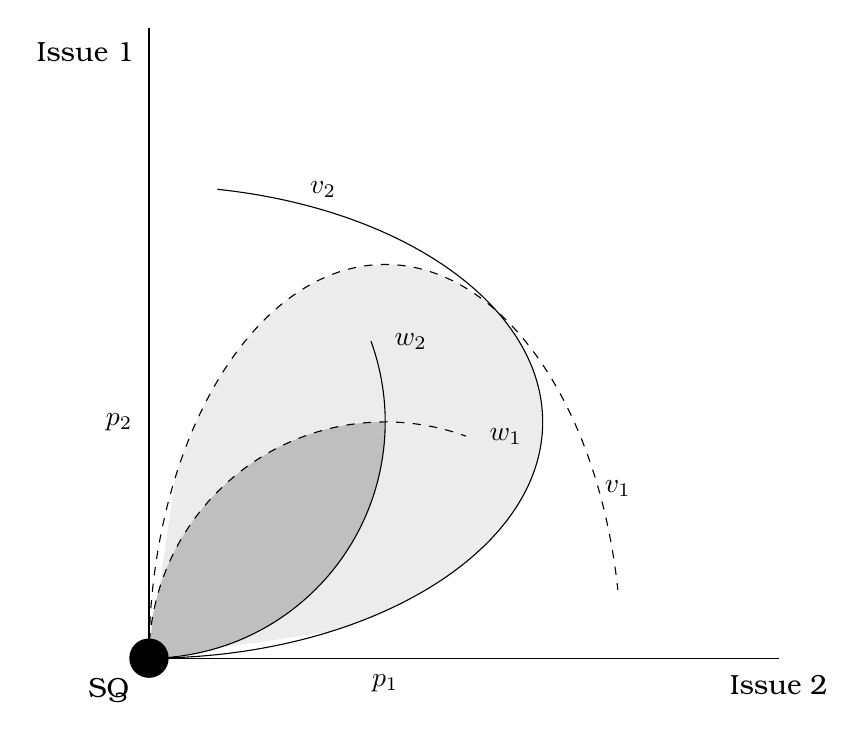
\begin{tikzpicture}
    \draw (0,0) -- (0,8) node [below left = .25em] {Issue 1};
    \draw (0,0) -- (8,0) node [below = .25em] {Issue 2};

    \begin{scope}
      \clip (0,0) arc (180:10:3 and 5);
      \clip (0,0) arc (-90:80:5 and 3);
      \fill [gray!15] (0,0) rectangle (10,10);
    \end{scope}

    \begin{scope}
      \clip (0,0) arc (180:10:3);
      \clip (0,0) arc (-90:80:3);
      \fill [gray!50] (0,0) circle (10);
    \end{scope}

    \draw [dashed] (0,0) arc (180:10:3 and 5) node [above = 3em] {$v_1$};
    \draw [dashed] (0,0) arc (180:70:3) node [right = .5em] {$w_1$};

    \draw (0,0) arc (-90:80:5 and 3) node [right = 3em] {$v_2$};
    \draw (0,0) arc (-90:20:3) node [right = .5em] {$w_2$};

    \node at (0,3) [left = .25em] {$p_2$};
    \node at (3,0) [below = .25em] {$p_1$};
    \fill (0,0) circle (0.25) node [below left = .5em] {SQ};
  \end{tikzpicture}
  \caption{A Two Dimensional Spatial Model}
  \label{fig:twodimensions}
\end{figure}

The winset when both issues are weighted equally by both actors is nested within the winset for when the issues are weighted differently. Thus when actors attach different saliences to different issues they are willing to accept a decrease in utility on one issue for a correspondingly greater gain in utility on a second issue, hence the possibility for striking a deal increases substantially. This is represented by the shaded areas in Figure \ref{fig:twodimensions}, where the darker shade marks the winset when both issues are weighted equally, and the lighter shade marks the winset when one dimension has a higher salience. 

The added value of this model is that it does away with the assumption of sincere voting, which was made in the simple one dimensional spatial model. The results from the two dimensional spatial model are often used when scholars want to explain the prevalence of unanimous decisions in the Council \citep{MattilaLane2001,KonigJunge2009}. However for log rolling to be possible certain conditions need to be fulfilled, first actors need to know each others positions and saliences attached to these positions. Secondly the saliences must differ across actors. If actors are uncertain or do not have access to information on positions and saliences then no log rolling can take place. Third, log rolling in the spatial model is simultaneous. If the votes on the different issues are separated in time then we need to assume that actors can make binding agreements, otherwise one actor will always be able to defect from the deal without incurring any penalties. However the further the votes are from each other in time, the more uncertain any actor will be about the positions and saliences of the others. Thus from a spatial point of view log rolling should take place either simultaneously or within a short time span. 

The spatial model has provided many insights into decision making in legislative bodies, however the model also displays several weaknesses with regards to decision making in the Council.  First of all the simple spatial model is a poor predictor of the level of conflict when the Council votes. The more sophisticated two-dimensional model with varying saliences fares better in this regard, and it does away with the assumption of sincere voting. However the two-dimensional model assumes that log rolling is done practically simultaneously, and thus do not allow for log rolling on situations where there is uncertainty with regards to the issues considered, or when there is a time gap between the consideration of issues. As Keohane has noticed, if only synchronous exchange is possible few agreements would be made, as issues often arise sequentially, hence an appropriate exchange may be impossible when only considering issues at one point in time \citep[21]{Keohane1986}. 

A particular weakness with the spatial models, indeed most formal models, is that they do not provide any clues as to why governments should resort to different types of dissenting votes. The spatial model only predicts whether a government should vote no or yes, however it does not address the issue of abstentions and no votes and how the meaning of these votes change with different voting rules. Spatial models do not necessarily exist in a binary world where governments are either in favor or not. It is conceivable that a criteria could be used to predict when a government would vote no or abstain, based on the distance from the ideal point to the likely outcome. However this challenge has not been taken up in the present research on the Council. When researchers use the spatial model to predict outcomes they make the implicit assumption that abstentions can be lumped together with no votes, this ignores a lot of information  

\section{Diffuse Reciprocity}

\citet{Keohane1986} has labelled the form of log rolling predicted  by the spatial model for specific reciprocity, i.e. an exchange of votes which do not carry any further obligations. He argues that when exchanges do not carry any future obligations only limited cooperation among actors is possible. In this sense synchronous log rolling cannot lead to stable patterns of cooperation. If log rolling is supposed to happen on issues separated in time then a different mechanism is needed. Keohane labels this diffuse reciprocity. The concept of diffuse reciprocity is based around the idea of future gains. It is assumed that actors care about future interactions with each other, and thus they have an incentive to engage in compromises in order to build up a ``favor bank'' which can called upon when the need arises \citep{Heisenberg2005}. Indeed diffuse reciprocity is modelled around a sequential bargaining model where concessions in bargaining exchanges do not have to be made simultaneously nor necessarily be strictly equivalent \citep{Jonsson2000}.  Just like the two dimensional spatial model with differing saliences among actors enlarged the winset, diffuse reciprocity enlarges the number of potential deals to be made by including future bargains into the considerations of actors. 

Within sociology and anthropology the idea of diffuse reciprocity has a long tradition. Starting with the study by \citet{Mauss1950} of the \textsl{potlach} tradition among north american indians and the study of the kula exchange ring among the trobriands of the western pacific by \citet{Malinowski1922}, it has been recognized that asynchronous exchanges contribute significantly to the stability of social systems. In the words of Gouldner:

\begin{quote}
  ``Insofar as we live under the such a rule of reciprocity, when one party benefits another an obligation is generated. The recipient is now \textsl{indebted} to the donor and he remains so until he repays. Once interaction is seen as taking place over time, we may note that the norm of reciprocity so structure social relations that, between  the time of Ego's provision of a gratification and the time of Alter's repayment, falls the shadow of indebtedness.''
\flushright{ - \citealt[174]{Gouldner1960}}
\end{quote}

\citet{Blau1964}, in his theory of social exchange, argue that once a donor-recipient relationship has been established a positive feedback mechanism is set in motion that require actors to further engage in asynchronous exchange relations in order to reap the benefits of the exchanges made. This fosters the development of a social structure in which reciprocity is a defining principle that regulate social interaction. What distinguishes social exchange from purely economic exchange is that economic exchanges are governed by a precise definition of any possible future obligations that might arise as a consequence of an exchange (such a taking a mortgage to buy a house), whereas social exchange involves a general expectation of a future return it is not precisely defined what this return might be. Thus social exchange creates diffuse future obligations, this requires a degree of trust in other actors that they will honor the obligations. It is therefor the inherent risky nature of social exchange relations that make the development of diffuse reciprocity possible \citep[94]{Blau1964}. The social exchange model proposed by Blau has been found to be effective in a number of contexts ranging from small businesses and political parties to experimental settings involving college students \citetext{for an overview see \citealt{CropanzanoMitchell2005}}.  

Many scholars have argued that specific reciprocity can under the right conditions transform into a stable system of diffuse reciprocity \citep{Gouldner1960,Axelrod1986,Keohane1986,NowakSigmund1998,Diekmann2004}. For instance Keohane follows Blau in arguing that when bargaining takes place sequentially there will always be an element of trust between actors. This trust element is found in the build up of a series of debts and credits, where the debtor has an incentive to default. However if there is a high chance of actors to meet again in future negotiations, the shadow of the future will weight heavy on the promises made. If the future is considered sufficiently important then the shadow of the future will outweigh the incentive to defect. This argument is supported by \citet{FehrFischbacherGachter2002} who argue that if the chance of two actors repeatedly interacting with each other is sufficiently high, actors will engage in reciprocal acts of cooperation. \citet{NowakSigmund1998} showed that a reputational mechanism can explain the efficacy of diffuse reciprocity. The crucial aspect of a reputational mechanism is the presence of an audience that witnesses the interactions that a given actor engages in. This allows actors to accumulate ``image'' scores for every cooperative action they make, thus making it more likely that other actors that are aware of their images will cooperate. Such a mechanism only works under the scope conditions that all interactions are done in public and all actors belonging to a group  have the possibility of gaining information on interactions by either observing them directly or by talking to other group members. This argument has also been taken up by Putnam who argues that diffuse reciprocity helps to amplify reputations of actors, and thus makes it easier to overcome dilemmas of collective action \citep{Putnam1995}. As \citet{Axelrod1986} points out, reputations serves as signaling devices, indicating which actors can be trusted in future negotiations an which actors are to be shunned. If an actor decides to default on an obligation this sends a signal to other actors, when a series of donor-recipient relations has been forged this can be very costly for the actor who defaults as s/he might not see any future return on the concessions made.    

Much like log rolling there are thus certain conditions necessary if diffuse reciprocity should develop. First of all actors need to be in an institutional environment in which they will on a regular basis interact with each other. When this condition is fulfilled the shadow of the future will show a strong presence. Furthermore \citet{Lewis2005} argue that actors involved in negotiations need to be in a relatively insulated setting, such that negotiations can take place free of domestic publics bearing witness. 

These scope conditions are to a large degree present in the Council. The permanent representatives meet on a frequent basis in the COREPER I and II committees, and the work of the committees is sheltered from any outside view. It has been shown in the literature on the Council that the frequent meeting activity has led to the rise of a bargaining culture where a vote is seldom pushed, but rather negotiations are carried on until either everybody is on board, or all possibilities has been exhausted \citep{Lewis1998,Lewis2003, BjurulfElgstrom2004}. Moreover the insulation of the COREPER committees allow national representatives  a degree of freedom to pursue deals that might otherwise not be considered by the minister at home, and present them as the best possible outcome \citep[947]{Lewis2005}. This type of consensus seeking bargaining relies heavily on a diffuse reciprocity mechanism. In order to reach a consensual outcome in the light of strong opposition from some governments, it is important that these governments can compromise on their positions and feel secure that they will somehow be compensated at a later date. 


\section{Diffuse Reciprocity and Signaling}

One apparent weakness of diffuse reciprocity, as outlined in this chapter, is the reliance on the recollection of previous negotiations, some often quite a while back in time. Representatives of governments in the Council have limited memories, and they do change from time to time, hence letting it be known that a government is compromising only through verbal agreement can be a risky strategy. Thus an instrument that records the disagreement is a very useful tool. The voting records in the Council is such a tool. Through the registration of a vote governments can leave a permanent record of their behavior. Given the tendency in the Council to have oversized majorities, the voting behavior of the individual government rarely will effect the outcome of a vote, and hence voting records are mainly useful as signaling devices.

Governments in the Council face two audiences, their domestic public and the other governments in the Council. Given that EU politics is seldom placed high on the public agenda, the domestic audience can in many instances be reduced to specialized interest groups. Any government must balance its behavior in the Council between being a credible coalition partner and not offending domestic interest groups. Whenever a government finds itself in the minority position in the Council it must decide whether to silently agree with the majority, somehow show its disagreement while still playing cooperatively, showing open disagreement to the members of the Council, or siding with a domestic constituency against the majority in the Council. Under QMV voting no and abstaining has the same effect, but arguably voting no to a dossier sends a stronger signal to a domestic constituency, which might not be familiar with the procedures in the Council. Other representatives in the Council are likely to grasp the difference, hence when governments want to show strong disagreement within the Council, but not necessarily to the public, abstentions will be the preferred signal. Therefor it makes sense to distinguish between no votes as signals to domestic constituencies and abstentions as signals to other colleagues in the Council. 

Under unanimity the situation is different, however the voting behavior can be interpreted as sending the same signals as under QMV. Any government is a veto player and can block a decision they are not satisfied with, although in praxis this is observed very rarely as most dossiers that cannot be passed in the Council are returned to the Commission to be redrafted. Thus we should only on rare occasions observe no votes under unanimity. Abstentions under unanimity cannot block a decision, thus they are equivalent to a government not being present for a vote and allow the other governments to proceed with the decision. Abstentions, though, do not encourage a decision either hence there is still a substantive difference between abstaining and voting yes. In this sense abstaining is equivalent to sending a signal of dissatisfaction to the Council. 

There is a third option which we have not broached so far. In the Council it is possible to attach statements to votes. Such statements can serve a number of purposes. They are frequently used to illuminate how a given government will interpret certain articles, or how the implementation might differ from other member states. The Council as a body do also frequently attach statements to votes that are typically directed at the Commission. One type of statements that are of particular interest from our point of view is the negative statement. Sometimes governments will attach statements to their votes explaining why they felt compelled to vote the way the did. When a government chose to record a dissenting vote, such statements often describe either fears that a given dossier will create a undesirable precedence within the Community, or that aspects of the dossier are viewed as detrimental to the interests of said government. More often than not governments will attach statements to yes votes detailing aspects that they are not satisfied with. These types of situations speak directly to the argument that governments build up favor banks within the Council, by showing that often governments will agree to vote affirmative to dossiers that they are not satisfied with. 

Finally voting yes in the Council can be interpreted in two ways, either a given government simply do not attach enough salience to a given dossier to raise any objections, or the final outcome is in agrement with the preferences of said government. This is a more complicated case as without information on the salience a given government attached to the dossier we cannot distinguish between the two reasons behind a yes vote. In any case voting affirmative in the Council is less interesting case as it does not provide any meaningful information with regards to signaling behavior. Based on these considerations Table \ref{tab:signaling} show a typology of Council voting behavior based on signal type, recipient and message.

\begin{table}[htp]
  \centering
  \resizebox{\textwidth}{!}{
  \begin{tabular}{l c l} \toprule
    Signal & Recipient & Message \\ \midrule
    No Vote & Domestic Constituency & Support of domestic interests against the Council \\
    Abstention & Council & Strong disagreement with the final outcome \\
    Yes + Negative Statement & Council & Support despite disagreement \\ \bottomrule
  \end{tabular}
}
  \caption{Types of Signaling in the Council}
  \label{tab:signaling}
\end{table}

In Table \ref{tab:signaling} only the third choice category is engaging in an exchange relation within the Council. When a government votes yes to a dossier in which it has reservations and goes through the trouble to make the Council aware of these reservations, it is difficult to explain this type of behavior from a spatial point of view. The simple one-dimensional model cannot accomodate any cases like this. The two-dimensional model is able to accommodate log rolling, however since log rolling is based on an already agreed trade it is difficult to explain why governments would feel the need to advertise their disagreement with the given dossier. The third category is, however, consistent with an explanation of negotiations in the Council based on diffuse reciprocity. Since governments make concession based on diffuse future rewards, it makes sense that they would want to remind their colleagues about the concessions made, and have a permanent record of the concessions. 
 
No votes and abstentions, on the other hand, should both be seen as deviating acts from the diffuse reciprocity mechanism. However deviations comes at a cost. Any deviation from diffuse reciprocity will diminish the number of favors that can be called upon at a later stage, and if done often enough it would put a given government at a severe disadvantage. Only in situations of either a severe domestic pressure or very strong preferences that are not accommodated by the Council would we expect to see governments compromise their standing within the Council. 


\section{Normative Behavior and Diffuse Reciprocity}

Diffuse reciprocity as defined above is closely associated with the rise of social norms. Indeed Lewis notes:

\begin{quote}
  ``[...] informal norms such as diffuse reciprocity operate in the context of COREPER's institutional environment and can promote pro-norm behavior.''
\flushright{- \citealt[964]{Lewis2005}}
\end{quote}

Most authors view diffuse reciprocity as an expression of a social norm \citep{Keohane1986,Lewis2000,Lewis2005,Diekmann2004}. However, before we can claim that diffuse reciprocity is a social norm we need to carefully define what a social norm is. When discussing norms there is an important distinction between private and social norms. Private norms refer to self-imposed standards governing only an individual, and usually sustained by feelings of guilt and/or anxiety \citep[100]{Elster1989}. Social norms, on the other hand, governs behavior within groups, and are sustained by approval or disapproval by the members of the group towards the actions of the individual. This general definition of social norms is widely shared in the literature \citep{Elster1989,Bicchieri1990,Coleman1990}, however when it comes to the specifics there are many differences. Coleman distinguishes between prescriptive and proscriptive norms, and Elster develops a complex classification scheme for different kinds of social norms. The most specific definition of a social norm is found in \citet{Bicchieri2006} who develops her definition around the idea of expectations and conditional preferences. According to Bicchieri we can define behavioral regularity $R$ in population $P$ as a norm if:

\begin{enumerate}
\item Almost every member of $P$ prefers to conform to norm $R$ on the condition that almost everyone else conforms too.
\item Almost every member of $P$ believes that almost every other member of $P$ conforms to $R$.
\end{enumerate} 

The same conditions that allow diffuse reciprocity to emerge also support the existence of social norms. Indeed diffuse reciprocity is based on the expectation that in the future the exchange will be reciprocated. In order for diffuse reciprocity to work this expectation has to be almost universally shared in a given group. Hence the way diffuse reciprocity is treated in the IR and EU literature aligns it closely with Bicchieris definition of a social norm. 

The advantage of Bicchieris definition of social norms is that it circumvents the problem of internalization. To illustrate this issue consider the popular ``three step model'' of norms \citet{Finnemore1998}. First a norm is promoted through norm entrepreneurs, if they are successful and reach a critical mass, a norm cascade will follow in which more and more actors adopt the norm, in the final step the norm is internalized and becomes habitual. In this model only norms that are successfully internalized will survive and become established modes of practice. Thus in the third step norms become habitualized and are no longer consciously used by actors. The main problem with a model that relies on the internalization of norms is that it makes norms hard to observe, precisely because of their ``taken-for-grantedness'' \citep[495]{Johnston2001}. Furthermore there is plenty of theoretical and empirical evidence that internalization of norms can happen, but is not a necessary condition for norms to thrive. Hence adding an internalization step to a model makes it more complex than need be. It is a long established result in the game theoretical literature that norms can come into existence through the interaction between actors, for instance in the classic tournament by conducted by \cite{Axelrod1986} a cooperation norm can be established simply through actors monitoring each other an adjusting behavior accordingly. Several mechanism are proposed that can sustain norms, among others: reputation and social proof. This is corroborated by Bicchieri who convincingly argue that the rise of a social norm is best viewed as a learning process. When actors engage with each other repeatedly, they build up knowledge of past interactions which can be used to form expectations of future interactions. In this sense social learning has a decidedly bayesian flavor where expectations are continuously updated based on the latest interaction. Hence a norm do not need to be internalized in order to be effective in structuring the behavior of actors.  This is in agreement with the many authors who find that there is a large degree of strategic thought behind normative behavior. \citet{Schimmelfennig2003} find that governments during the debate about eastern enlargement would invoke constituent norms of the EU, such as inclusivity, to further their cause. The same pattern has been observed in the US Supreme court, where the chief justices Marshall and Hughes both used the ideal, that the highest court in the US should present a unified front to the public strategically to ensure unanimous voting decisions \citep{CalderiaZorn1998,Epstein2001}.  


\section{Measuring Diffuse Reciprocity}

In the social sciences social norms have featured prominently in many theories, however when empirically testing social science theories finding an appropriate indicator for normative behavior has not been easy. Two approaches have achieved some prominence. First of all many game theorists have devised different types of games to elucidate normative behavior, typically these games have been used in laboratory settings, where the conditions for normative behavior can be controlled. Based on insights from these experiments one set of authors have devised an approach that involves identifying behavior that is at odds with the preferences of actors. Another set of authors have looked towards the econometric literature on co-integration \citetext{see \citealt{Beck1992}}, and argue that consensus norms regulate conflictual behavior, and if we can identify and underlying factor regulating conflictual behavior, then we have corroborative evidence for the presence of a norm. 

When assessing the causal impact of norms, researchers has often turned to devising experiments under which the conditions for normative behavior can be controlled in an exact manner. In the experimental game theory literature a number of experiments have been devised to elucidate different types of pro-norm behavior ranging from altruism to conditional cooperation. Particularly public goods experiments have yielded interesting insights into how norms are sustained in small groups A common experiment is to let two players play a prisoners dilemma game, where if they cooperate the good is provided and they each share the cost, if one defects the other actor will bear the burden of providing the good. To this setting a neutral observer is added who could decide to punish players at will. Punishment is costly, however, and whenever the observer decided to punish a small cost was incurred. Results from these experiments show that often third parties decide to punish actors that defect, thus lowering the payoff associated with defection \citetext{see \citealt{FehrFischbacher2004} for an overview}. These experiments illustrate that acting normatively often means compromising on pure utilitarian goals, i.e. when the chance of getting caught is high and punishment probable if caught, actors will choose to cooperate. Hence the empirical implication of these experiments is that to observe normative behavior we must identify situations where actors in public settings will act against their own selfish interests.  

This approach, which we can label the direct indicator, has been taken up by \citet{EpsteinSegalSpaeth2001} in their study of the US Supreme court. In the years 1800 to 1942 the US Supreme court had a yearly average of 91.5\% consensual decisions. This is in stark contrast to the period after the second world war, where disagreement has been the rule, not the exception.  Many scholars have argued that there were a norm of consensus present in the Supreme court, however conclusive evidence has been scarce \citep{Haynie1992,EpsteinKnight1996,CalderiaZorn1998,Epstein2001}. \citet{Epstein2001} propose that in order to establish the presence of a norm, one must be able to identify one type of behavior that is only consistent with a normative based explanation. This allows a researcher to dispose with alternative explanations that might produce the same outcome, but through a different mechanism. The approach taken by \citet{Epstein2001} was to identify cases in which judges had expressed doubts about a ruling in private, but still voted with the majority in public.  They argue that:

\begin{quote}
  ``This is precisely the sort of behavior we would expect to find if a norm of consensus operated on the Court; public unanimity masking private disagreements.''
\flushright{- \citealt[365]{Epstein2001}}
\end{quote}

This type of argument is very much in line with the evidence presented in the experimental game theoretic literature on normative behavior, i.e. we can recognize normative behavior when actors engage in costly behavior that is against their own utilitarian preferences. In the Council we have a direct equivalent to the indicator used by Epstein et al. Although the representatives of the governments do not record in detail their discussions, their use of statements attached to their votes indicate whether they acted against their short term interests. On many votes where member states votes yes, we see statements such as the following attached.

\begin{quote}
  ``The Spanish delegation states its disagreement with the distribution of EU TACs in the North Sea and the Baltic Sea areas. Spain maintains the appeals it has made to the Court of Justice of the European Communities against Regulations (EC) Nos 2341/2002 and 2267/2003, under which Spain was granted no quotas in those fishing areas despite the transition period’s having ended, and it will submit a further appeal.''
\flushright{Spain, COM (2004) 785}
\end{quote}

The above quote is taken from the vote on the regulation fixing the fishing quotas for 2005 in waters where catch limitations are required.  During the Spanish and Portugese accession negotiations a transition period was determined where fishing fleets for the two member states where not allowed to fish in the North and Baltic seas. This transition period has already expired, however since Spain commands the largest fishing fleet in the EU other member states have been reluctant in granting the spanish fleet fishing rights i their waters. However despite the efforts of Spain to secure fishing rights in the North and Baltic seas, the spanish government still voted yes to a proposal that did not grant them these rights. The dossier was adopted under QMV, so there was little to be gained from voting no, beyond sending a signal to the Spanish fishermen. Since Spain at the time had a series of appeals running at the European Court of Justice, one could argue that the fishing lobby had been appeased, hence voting yes on this dossier is difficult to explain from a spatial bargaining model, however it  is consistent with an explanation focusing on diffuse reciprocity. 

The second approach, which we can label the indirect indicator, to measuring norms has primarily been used within the IR literature \citep{RajmairaWard1990,RajmairaWard1992, Goldstein1991,Rajmaira1997} and the study of the US Supreme court \citep{CalderiaZorn1998}. The early move within the IR literature to assess the empirical presence of norms was very much influenced by the work of \citet{Keohane1986} and \citet{Axelrod1986}. The authors in the field commonly argue that norms should be viewed as social institutions. As such the purpose of a norm is to structure interaction among participants whenever there is the potential for conflict. Following the classic exchange theorists they argue that social institutions represent equilibrium points, and these equilibrium points are the result of a series of exchanges between actors. Social institutions must be able to engender compliance, otherwise they would not exist for long. In equilibrium compliance can be achieved in two ways. First of all it might be that no actor has any incentive to leave the equilibrium, i.e. to break the norm. The equilibrium point is then the optimal course of action. In this sense norms can be largely self-enforcing. Secondly, norms as institutions can provide reasonable expectations towards the behavior of other actors in certain circumstances. As such a norm will drastically lower the uncertainty that is associated with calculating consequences of possible avenues of action. Finally a norm can come with a sanctioning mechanism. If participants have the possibility to monitor social interactions and detect defection from the rule, sanctioning defectors allows a social institution to be upheld, despite not being the optimal course of action for all participants. In line with the literature on the consensus norm in the Council, all scholars stress the importance of time when dealing with norms. Social settings in which the actors interact frequently, where there is little replacement and socialization takes place by learning from more experienced actors, we can expect a long institutional memory to persist. It is under these conditions that we would expect norms to emerge, and the claim is that we can witness manifestations of norms in the behavior of participants in a social institution over time. The authors argue that a consensus norm should operate by regulating the amount of dissent expressed openly, furthermore this regulation of dissenting behavior should be present in a long time series. To assess this empirically scholars have conceptualized normative behavior as reactive sequences over time. For instance \citep{RajmairaWard1990,RajmairaWard1992} examine Soviet-US relations through the joint-event history of the two superpowers, by coding actions as either reciprocal or conflictual they examine the two time series to see whether they share an underlying component. If the two series tend to drift in the same direction, allowing for short term fluctuations, this evidence of a shared norm of reciprocity. Rajmaira \& Ward find this relationship to be strong in super-power interactions, an show that the past history of interactions are important in forming future expectations. Depending on the history this can lead to either long-term cooperation or conflict, as expectations become self-fulfilling. A similar pattern has been found in the US Supreme court by \citet{CalderiaZorn1998}. In the Supreme court judges have three possible choices when casting their vote, they can vote yes, no or write a concurrent opinion in which a judge expresses his/her agreement with the majority, but with different reasons as the basis for the decisions. Calderia \& Zorn argue that if a consensus norm is present in the Supreme court, then it should express itself in a consistent low level concurrences and dissenting votes, and both series should be governed by the same underlying factor. They find a strong relationship between concurrences and dissenting votes. This is interpreted as evidence for the presence of a consensus norm. This approach to measuring norms as the underlying factor the binds together long term trends in behavior that is consistent with normative expectations, carry a high potential for research on the consensus norm in the Council. Very much like the US supreme court, the copiously large amount of consenting votes have been interpreted as evidence for a consensus norm. In order to determine whether it really is a consensus norm that governs the high number of yes votes, the literature on norms in IR and the US Supreme court show that we can gain much by focusing on the relationship between types of dissenting votes. 

What type of norm the approaches outlined above capture is not clear. One assumption made in all studies is that we can identify one area of interest which should be governed by a single norm. Both Epstein et al. and Calderia \& Zorn assume that there is only one norm operating within the Supreme court, namely a consensus norm. In the same vein Rajmaira \& Ward assume that their tests capture a norm of reciprocity. In this chapter I have argued that a norm of diffuse reciprocity is the most likely explanation for the consensus seeking behavior in the Council,  this implies that any evidence found of normative behavior in the subsequent chapters will be interpreted as corroboration that a norm of diffuse reciprocity is active in the Council. 

\section{What to Come}
This chapter laid out the micro foundations for a theory of diffuse reciprocity within the Council. By showing how diffuse reciprocity can come into existence through exchange relations, and once established can lead to asynchronous log rolling, the foundations for an explanation of consensual voting in the Council relying on informal norms and methodological individualism was specified. Under a regime of diffuse reciprocity where any single vote will rarely make a difference, and governments use different types of dissenting that are formally equivalent, treating votes as signaling devices provides a possible explanation of the voting patterns that has been observed in the Council.  

In the next chapters the theory developed here will be explored with regards to three different aspects of decision making in the Council. Chapter \ref{chapter:votechoice} will examine the determinants of vote choice in the Council. A key aspect of the diffuse reciprocity approach to negotiations in the Council is the vote choice of the member states governments, if these choices are indeed signaling devices then we should be able to explain the vote choices as functions of domestic concerns, governments preferences and council composition variables.

In chapter ?? we will utilise the direct indicator, to determine the effect of diffuse reciprocity on the decision making speed of the Council. Several pieces have suggested that diffuse reciprocity has an effect on decision making time, if these claims are correct we should be able to explain decision making time as a function of diffuse reciprocity.

Chapter ?? will examine the time dependent aspect of diffuse reciprocity through the indirect indicator uncovered above. DIffuse reciprocity is build around the idea of asynchronous exchanges, hence time is a crucial aspect of the theory. Over time we should expect that the norm of diffuse reciprocity is effective in keeping dissenting votes at consistently low levels in the Council. Following the indirect indicator approach this translates into treating abstentions and no votes as two time series that share a common regulating factor. 

For each chapter the theory is extended and testable hypotheses are developed based on the premised laid out in this chapter. 



\chapter{Determinants of Vote Choice}
\label{chapter:votechoice}

\lettrine{T}{he} Food Flavoring directive adopted in 2008 was a controversial dossier. Especially Germany had issues surrounding the levels of allowed additives derived from aromatic spices and herbs. The dossier was adopted unanimously in the Council, but the German government attached the following statement to their vote. 

\begin{quote}
  ``Germany would have preferred a lower coumarin limit for traditional and seasonal bakery ware containing cinnamon the the one now provided for, but in a spirit of compromise can nevertheless support the proposed maximum level''
\flushright{ - Council Monthly Summaries October 2008 p. 21}
\end{quote}

 The dossier had been debated in the Council and parliament since 2006 and the parliament had significantly strengthened the scope of text from the Commission. Among other things, the Parliament proposed to leave an annex regarding the risk of using certain aromatic herbs and spices open until further evidence could be provided to determine the appropriate risk levels. This was welcomed by Germany which had argued that the levels set in the Commission proposal with regards to cinnamon were too high. However the Parliaments amendments was met with opposition from other governments in the Council, who feared that traditional artisans that produced bakery goods with cinnamon would be unnecessarily burdened by a lower limit.  Recognizing that the Council could not reach a decision the Commission withdrew the proposal, to redraft it. After several debates in the Council Germany agreed to give in on its reservations. 

The voting behavior of Germany on the Food Flavoring directive represents a case where  ....

This sort of behavior is an aspect of decision making not captured in current studies of the Council.  Most studies so far only examine yes votes, no votes or abstentions, thus situations like the one above where Germany expressed strong reservations about the legislation, but still voted yes, are not captured. Including cases like the one above thus allows us to study voting behavior in a more fine grained manner.

It is a commonly used explanation whenever a pattern of consensus is found in the Council to refer to the consensus norm, and often the high degree of unanimously adopted dossiers in the Council is used as corroborating evidence. However using unanimously adopted decisions as evidence for a consensus norm is not without pitfalls. There are many reasons for why a dossier was adopted unanimously. A dossier could be uncontroversial, thus requiring no need for seeking consensus. It is also possible that the preferences where so aligned that an agreement was reached without needing to resort to long negotiations. Finally it might be that logrolling was the mechanism. 

The cases of inflating a data set with uncontroversial dossiers or dossiers where the preferences were aligned can be remedied at the case selection stage. To distinguish between logrolling and diffuse reciprocity it is argued that behavior of the type exhibited by Germany above can be interpreted as engaging in diffuse reciprocity, by building up the ``favor bank''. 


\section{Diffuse Reciprocity and Voting in the Council}

Social norms offer consideral scope for interpretation, manipulation and choice. To treat norms as monolithic entities that determine social interactions is to revert back to the fallacy of the over-socialized actor that has plagued much of constructivist theory, however to treat norms purely n as tools to mask self-interest is to make the fallacy of the under-socialized actor plaguing much of rational choice theory \citetext{see \citealt{Elster1989} and \citealt{Schimmelfennig2000} for good overviews and critiques}. The theory of diffuse reciprocity is based around the notion of unanticipated consequences, as exchanges aquire a decidedly social flavor, actors get caught up in the emerging system of debts and credits. It is important to keep in mind that at no point are actors aiming towards such a system, it is an emergent phenomena resultant from the interactions in a social system. Since diffuse reciprocity do not rely on the internalization of a social norm, it is closer to a social equilibrium in which most actors would be worse of if they engaged in off equilibrium behavior. In such a system it is always a possibility that a government choose to pursue its own interest in hope of some short term gain, if the expected gain is higher than the expected long term loss in standing. The pertinent question raised here is when will a government decide to deviate from the exchange system, and pursue its own narrow interests. Drawing upon the work in chapter \ref{chapter:theory} we can label the incentives to defect in two categories, namely domestic concerns and preferences. These two categories are not entirely mutually exclusive, it is possible that domestic concerns will align with strong preferences against the final outcome. Furthermore the two categories are roughly correspondent to the classic concerns over whether politicians are mainly driven by the wish to succeed electorally, or to influence policies \citep{Strom1990}. There is evidence for both types of motivations in the literature on coalition formation, for instance \citet{MartinStevenson2001} show that parties, when deciding with whom to create a coalition, will show concerns for which office they will hold and the policy content of the coalition. In the Council concerns about electoral success can manifest themselves when domestic politics and EU legislation collide. This can often put governments in delicate situations where they must choose between being good members of the EU and appeasing domestic constituencies. The trouble of the reintroduction of the border control at the Danish border is illustrative in this regard. As part of a domestic settlement the Danish government agreed to introduce a limited border control in order to get the votes from the nationalistic Danish Peoples Party (DPP). Since Denmark is a member of the Schengen area, the implementation could only be very limited if should be complient with Schengen rules. However at home the DPP was claiming that the border controls would be a return to the border control that was in place befor Denmark joined the Schengen area \citep{Olsen2011,Euractiv2011}. This put the government in a difficult position where it had to choose between either downplaying the role of the border control, which would offend the DPP, or going along with the DPPs claim which would offend the Commission. 

Governments in the Council face two types of domestic constraints. One type can be labelled interest group pressure, and is distunguished by strong interest groups pushing an agenda at the EU level that is not necessarily in line with the preferences of the government. Lobbying has long been part of negotiations in Brussels. Lobbying typically display a pattern where national interests, organized in an umbrella organization, will go through their European counterpart to influence policy makers in Brussels. However often national umbrella organizations will also contact the relevant national ministers directly in order to convince them to push an agenda in the Council \citep{Beyers2002}. Most often interest groups will focus their attention on changing parts of the legislative text that they are not happy about, however when these efforts have proven futile the focus might be on recommending a government to vote no as a signal of support for domestic concerns. This has the effect of building relations between key constituent groups domestically, but will lower the standing of the government in the Council. The other constraint can be labelled public opinion. If a dossier at the EU level catches the eye of the public in a member state, it can have an impact in the re-election concerns of governments, particularly on EU sceptic member states such as the UK and Denmark. An interesting dynamic that has often been observed in the Council is blame shifting. In multilevel systems it is easy for institutions at at given level to engage in blame shifting and credit taking for political outcomes \citep{Anderson2006}. This has been observed in member states where governance is divided between different administrative structures, such as France and Germany \citep{Elgie2006}. It is no surprise that the same dynamic has also been oberserved to take place between member states governments and the EU \citep{Franchino2004}. If governments find themselves under pressure domestically, but are unable to block legislation at the EU level, it is tempting to vote no in order to appease the domestic audience, and blame the EU for forcing unwanted legislation. 

In the absence of domestic constraints, governments migh find themselves highly disagreeing with the outcome. The theory of diffuse reciprocity will predict that in these situation, the vote choice is dependent upon how much the future is weighted. If an actor has been very active in maintaining exchange relations then the future is weighted heavily, thus we would expect this actor to compromise. However actors that are not active in the system of exchanges will not weight the future very heavily, hence we will expect these actors to vote more along their preferences. This line of argument has been developed by \citet{HoylandHansen2010}. They argue that the consensus norm in the Council can be viewed as the propensity to override once own preferences in favor of a consensual decision. They are thus in line with the direct indicator approach specified in chapter \ref{chapter:theory}. In order to further specify this mechanism the authors use a spatial model with an added term to capture any effect of a consensus norm. Assuming that actors operate in a one-dimensional space with a linear loss function, the principle of utility maximization implies that an actor $i$ will vote yes to a dossier if:

\begin{equation}
  \label{eq:1}
  U_{ik}(-|x_{ik} - p_k|) < U_{ik}(-|x_{ik} - q_k|)
\end{equation}

Where $U_{ik}$ is the utility of actor $i$ on dossier $k$, $x_{ik}$ is the ideal position of actor $i$ on dossier $k$, $p_k$ is the position of the proposed dossier and $q_k$ is the status quo. Equation \ref{eq:1} thus represents the classic spatial model, to account for the effect of the consensus Hoyland \& Hansen add a third term, $\theta$, which is added in linear fashion to the loss function. Hence:

\begin{align}
  \label{eq:2}
  U_{ik}(-|x_{ik} - p_k|) > U_{ik}(-|x_{ik} - q_k|) &= No \\
  U_{ik}(-|x_{ik} - p_k| + \theta_i) < U_{ik}(-|x_{ik} - q_k|) &= Yes
\end{align}

Theta, if positive, will have the effect of reversing the vote, whereas if set to zero or a negative value will have no effect. According to \citet{HoylandHansen2010} if theta is constant across actors this will be evidence of a norm, however the theory of diffuse reciprocity will expect that there is variation in theta, as it more accurately reflects the degree to which a given actor is embedded in an exchange system. The authors do indeed find that theta varies significantly across member states in the Council, this is interpreted as evidence against a consensus norm, although it fits with the theory of diffuse reciprocity. The modified spatial model presented by Hoyland \& Hansen helps to illuminate some of the dynamics that could explain the effect of the consensus norm. However, like the spatial models covered in chapter \ref{chapter:theory}, the approach can only explain the choice between voting yes or dissent. The model do not provide any clue as to why some governments will abstain or vote no on dossiers. What we can learn from the model is that in the presence of a positive theta, only a strong disagreement with the final outcome will result in a government choosing a dissenting vote. 

Based in the above considerations we can formulate the following hypotheses:

\begin{quote}
  H1: When there is domestic pressure governments will vote no on a given dossier
\end{quote}

\begin{quote}
  H2: When governments are preference outliers they will abstain on a given dossier
\end{quote}

The social environment is an important aspect of diffuse reciprocity. Only when actors meet and interact on a regular basis can we expect to see a norm of diffuse reciprocity develop. This is often referred to as a process of social learning. In its most simple form this process assumes what \citet{Skyrms1997} has called Markov agents, i.e. actors that only use the immediate past to adapt their behavior. Social learning in this context is defined by actors interacting and then updating their beliefs about other actors which might lead to a change in their behavior. If this process is run for a long enough period of time, then the interactions will settle on a specific pattern, and we say that the social system has converged. If we assume that actors memory stretches further back than just the immediate past we get actors that condition their future expectations on the past behaviors of their colleagues, which in small groups with a stable membership can lead to the emergence of diffuse reciprocity. The starting point of this causal chain is the interaction frequency, which is a key variable to account for. This opens up the possibility that a norm of diffuse reciprocity might be present to different degrees in different policy areas based on the meeting frequency of the Council configurations. In policy areas where the Council configuration only meet in-frequently we would expect the norm of diffuse reciprocity to be less strong than in policy areas where the Council configuration meet frequently. For instance in 2010 the General Affairs Council meet 16 times while the Economic and Financial Affairs Council (ECON) meet 29 times, hence we would expect that the norm of diffuse reciprocity is more present in the ECON configuration. In voting behavior this would manifest itself in fewer instances of governments voting yes to dossiers, but attaching dissenting statements to their votes. This leads to the following hypothesis:

\begin{quote}
  H3: The higher the meeting frequency the more often we will see governments attaching dissenting statements to yes votes
\end{quote}

%a social dilemma: vote along with preferences for an immediate benefit, or vote against for a diffuse long term benefit. 

%The role of the social environment

%what determines vote choice

\section{Research Design}

\subsection{Case Selection}

In order to test hypotheses about voting behavior in the Council it is important to have the proper universe of cases. In most studies of voting in the Council the focus has been on either the entire population of cases, typically aggregated in some fashion. This ignores the possibility that there might be a great number of dossiers in the Council that are mainly technical, and thus do not engender any deal of controversy from the member states government. In these non-controversial cases we should expect the Council to exhibit perfect cohesion with regards to voting. From our perspective these cases are also not interesting as only in cases with some degree of controversy do we expect the norm of diffuse reciprocity to be active. Hence it is important to be able to distinguish between cases in which the preferences of member states are all aligned, from cases in which there was some degree of disagreement within the Council. Indeed including these cases in the analysis risks biasing the analysis towards finding evidence for a high degree of consensus, and hence stack the deck in favor of a consensus reading of the Council. 

The first step in the analysis is to define the population of relevant cases. In our case the population is defined as dossiers treated in the Council where there was disagreement about the final outcome. In the literature on decision making in the EU several criteria has been used to separate controversial from uncontroversial dossiers. It has been common in the voting record literature to analyze cases on which there was a dissenting vote separately \citep{Heisenberg2005,Hayes-renshaw2006,Hagemann2008}. However this introduces selection bias if the dependent variable is the vote choice of the member states. The DEU project \citep{Thomson2006a} used the criteria of public reporting. If an act was mentioned in Agence Europe it was considered as being controversial. This approach has the drawback that it is not possible to discern whether this controversy represented divisions within the Council, or disagreements between constituent groups and the decision reached by the Council. In order to avoid this ambiguity I will use a more direct measure of controversy within the Council. The cases used in this paper are selected on the basis of having, at one point, been treated as a B-point in the Council.

The Council agenda distinguishes between A and B points, where A points are dossiers that do not require discussion at the ministerial level, and B points are dossiers in which no agreement could be reached on working group level and need discussion at ministerial level. It is common practice in the Council that issues that are discussed as B points are afterwards send back to the COREPER for a final drafting and than at a later date adopted as an A point in the Council. In recent years several scholars have noted the presence of ``false B-points'' \citep{Lewis1998,hage2008,Muehlbock2011}. These are dossiers where agreement has already been reached at a lower level, but are discussed at the ministerial level to allow a minister to make an oral statement. These statements can be used to voice reservations against the dossier, or might be intended for a domestic constituency. Hence from the point of this chapter ``false B-points'' do not represent a problematic category. The same authors also mention the presence of ``false A-points''. These are cases where a dossier is adopted as an A-point, but was at some stage discussed as a B-point in the Council. This implies that if we only focus on dossiers that were adopted as B-points we would miss a great number of controversial cases. To account for this the selection rule developed above selects cases that at any point during their treatment in the Council was discussed as B-points in the Council. 

The advantage of selecting only cases treated as B-points in the Council is that we are sure to select cases in which there were some controversy related to differences within the Council, and the selection rule does not restrict the variance on the voting outcome. This make it possible to mitigate any potential bias by including non-relevant cases. 

A word on the unit of analysis is warranted here. Most studies of the Council have the member state as the unit of analysis, this obviously leads to conclusions on the member state level as well. In some instances where we can expect the preferences of member states to be constant despite changing governments, this is an appropriate unit of analysis, however if we can expect the behavior of delegations in the Council to change as the parties in office change then the assumption is problematic. The natural unit of analysis in the Council is the present government in office, this implies that besides having variation between member states, we can also expect to observe variation within the individual member state as governments change. Ignoring this variation can have quite dramatic effects. To see how this can effect the analysis of voting behavior in the Council consider Sweden. During the third installment of the social democratic Persson government, Sweden had 28 dissenting votes, thus placing the Persson III government among the most dissenting governments in the 1999 - 2009 period. Compare this to the successor government, the liberal Rheinfeldt government, that only registered a dissenting vote 8 times. The Persson III government was in power for 1446 days, and the Rheinfeldt I government for 1460 days, hence the difference is unlikely to be caused by a sudden bias in the Commission proposals. However the governments differed significantly in how much they deviated from Council median left-right position. The Persson III government had a deviation of 2.27, whereas the Rheinfeldt government only had a deviation of 1.24. Hence the difference in the dissenting behavior can most likely be attributed to ideological differences with the other member states governments. If we were to ignore this and simply lump both governments together as being Sweden, then we would wrongly classify sweden as being a middle of the road member state, while ignoring the great differences in Swedish governments behavior in the Council. Thus the natural unit of analysis when trying to explain Council voting behavior are the governments of memberstates. 


\subsection{Data and Variables}
The dataset used in this paper cover the years 1999 to 2009 and includes every vote in the Council during this time period. In total there are votes registered on 3937 dossiers, which gives a total of 78968 votes cast by member states governments. Of these 16473 where cast for dossiers that at one point was a B point in the Council. Beside the vote cast, the data also contains information on whether a statement was registered by any member state, and whether this statement expressed dissatisfaction with the outcome. This coding is more fine grained compared to most studies who either ignore the possibility of registering a statement in conjunction with a vote, or simply code whether there was a formal statement or not.

The focus of this study is the voting behavior of the member states in the Council of the EU. As such the dependent variable is the individual vote choice of the government in power in a given member state. There are three vote choices available to any member state, namely yes, no or abstain. These choices are coupled with the possibility of also registering a statement in conjunction with the vote. Since the theoritical interest is centered around yes votes with a negative statement, the votes have been split into four categories:

\begin{enumerate}
\item Yes
\item No
\item Abstain
\item Yes + Statement
\end{enumerate}

Here we have only included the statements that express dissatisfaction with the final outcome. Thus the dependent variable reflect one category of agreement (yes) and five categories of different types of dissent. It is difficult to rank vote choices, they represent different choices which do not have a well defined high and low point according to which they can be ranked. For this reason the variable is treated as being nominal in this paper. 

The independent variables are measured on two levels, namely the dossier level and the member state government level. The member state government is the lowest level in the data, and are nested with the dossier level, such that for each dossier we have recorded between 15 and 27 votes that are attributed to governments from the member states. Table \ref{tab:variables} show the variables along with the source and descriptive statistics. 




\section{Descriptive Evidence}
As a first look at the data table \ref{fig:depvar} show the distribution of votes across Council Configurations. The number of yes votes, have been left out as they dominates the distribution. Even after having selected only definitive legal acts that where treated as B points in the Council, the number of yes votes is staggering. The second largest category is abstentions. The third largest category, in most Council is a yes vote with a dissenting statement attached. This show that studies not taking Council statements into account risk biasing their findings towards consent. The prevalence of attaching negative statements to supporting votes suggests that there is a large degree of signaling behavior going on in the Council. It is important to let your colleagues know that you are a team player and willing to compromise. This speaks for the interpretation of negotiations in the Council as oriented towards diffuse reciprocity. It is also striking that dissenting behavior is not equally distributed across Council configurations. Agriculture\& Fisheries, Competition and Employment, Health \& Consumer Affairs exhibit a very high degree of dissent when compared to the other Council configurations. Thus we clearly see some policy specific effects on voting.

\begin{figure}[htp]
\centering
\scalebox{.6}{% Created by tikzDevice version 0.6.1 on 2011-08-03 09:50:49
% !TEX encoding = UTF-8 Unicode
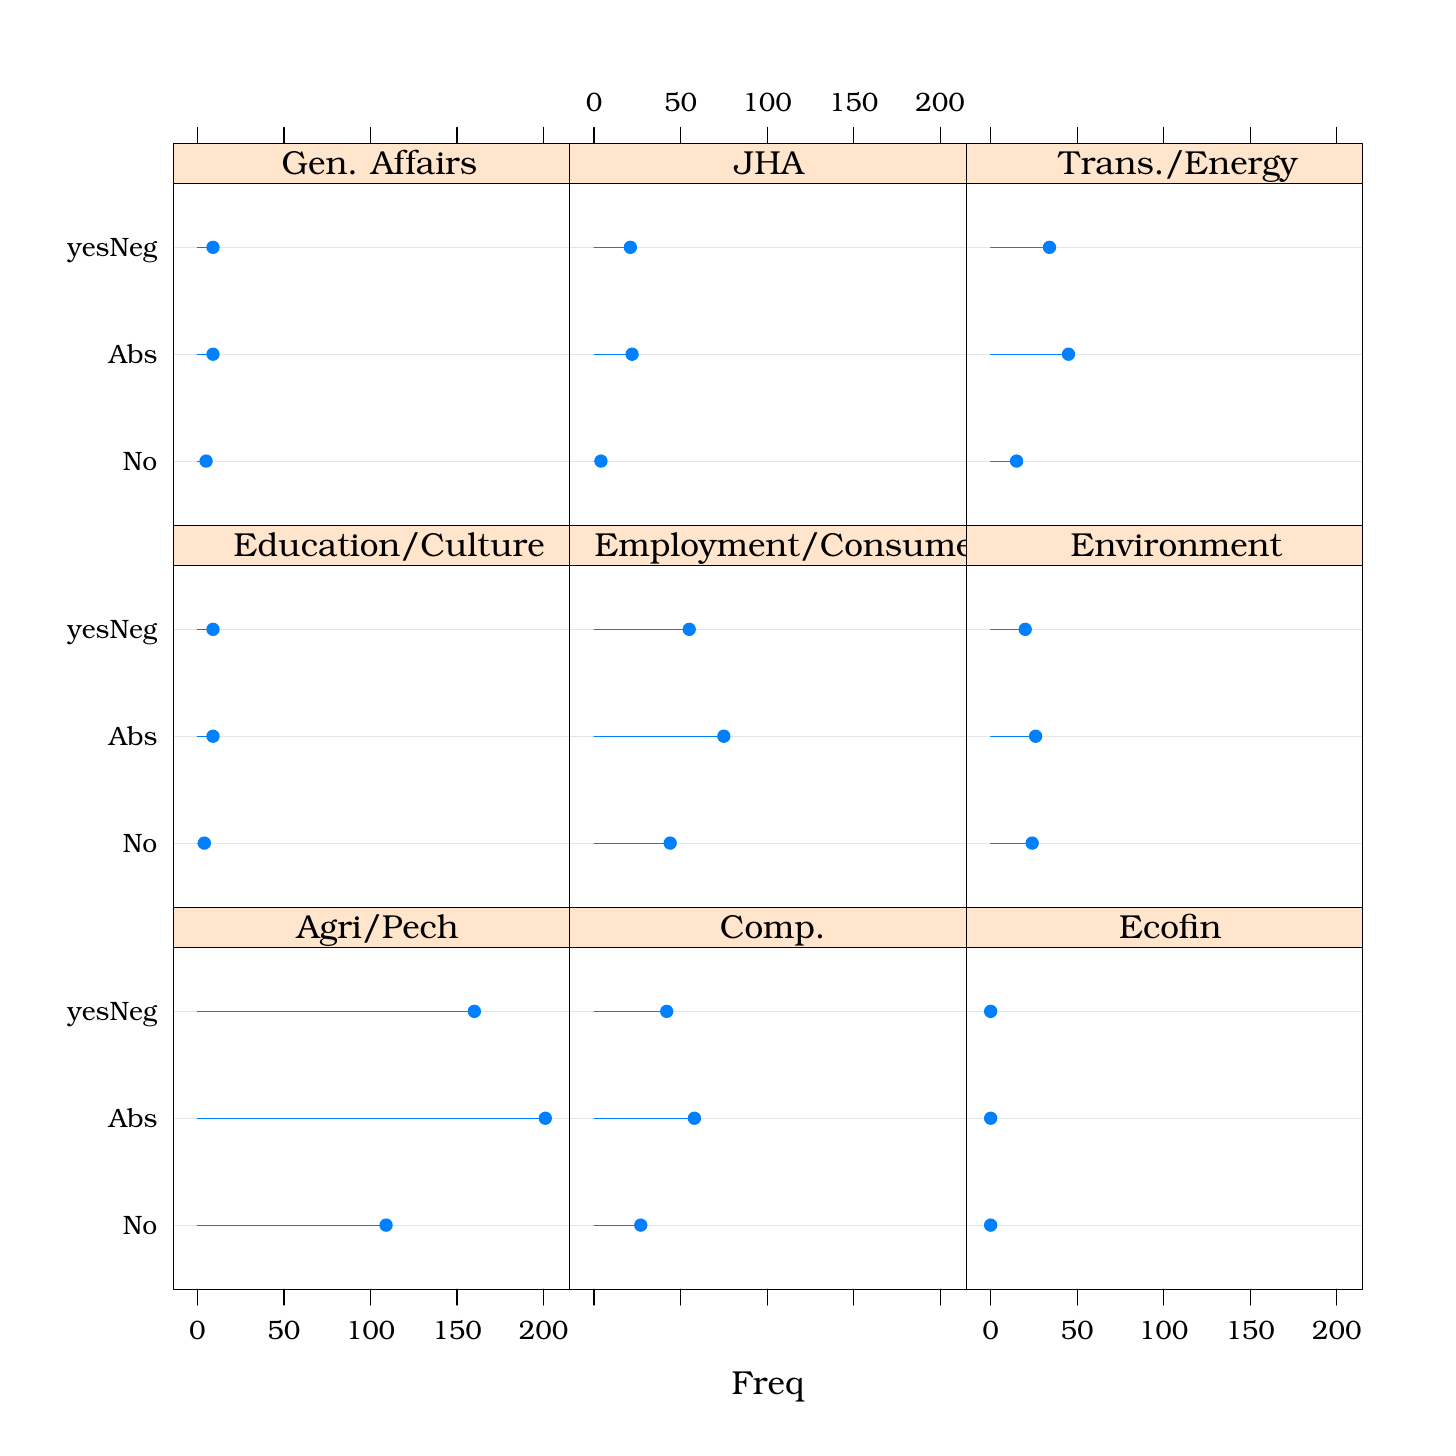
\begin{tikzpicture}[x=1pt,y=1pt]
\definecolor[named]{drawColor}{rgb}{0.00,0.00,0.00}
\definecolor[named]{fillColor}{rgb}{1.00,1.00,1.00}
\fill[color=fillColor,] (0,0) rectangle (505.89,505.89);
\begin{scope}
\path[clip] (  0.00,  0.00) rectangle (505.89,505.89);
\definecolor[named]{fillColor}{rgb}{0.00,0.00,0.00}
\end{scope}
\begin{scope}
\path[clip] (  0.00,  0.00) rectangle (505.89,505.89);
\definecolor[named]{fillColor}{rgb}{0.00,0.00,0.00}

\draw[fill opacity=0.00,draw opacity=0.00,] (  0.00,  0.00) rectangle (505.89,505.89);
\definecolor[named]{drawColor}{rgb}{0.00,0.00,0.00}

\node[color=drawColor,anchor=base,inner sep=0pt, outer sep=0pt, scale=  1.20] at (267.50, 12.04) {Freq%
};
\end{scope}
\begin{scope}
\path[clip] (  0.00,  0.00) rectangle (505.89,505.89);
\definecolor[named]{fillColor}{rgb}{0.00,0.00,0.00}
\end{scope}
\begin{scope}
\path[clip] (  0.00,  0.00) rectangle (505.89,505.89);
\definecolor[named]{fillColor}{rgb}{0.00,0.00,0.00}
\end{scope}
\begin{scope}
\path[clip] (  0.00,  0.00) rectangle (505.89,505.89);
\definecolor[named]{fillColor}{rgb}{0.00,0.00,0.00}
\end{scope}
\begin{scope}
\path[clip] ( 52.54, 50.02) rectangle (195.85,173.60);
\definecolor[named]{fillColor}{rgb}{0.00,0.00,0.00}
\end{scope}
\begin{scope}
\path[clip] (  0.00,  0.00) rectangle (505.89,505.89);
\definecolor[named]{fillColor}{rgb}{0.00,0.00,0.00}
\end{scope}
\begin{scope}
\path[clip] (  0.00,  0.00) rectangle (505.89,505.89);
\definecolor[named]{fillColor}{rgb}{0.00,0.00,0.00}
\end{scope}
\begin{scope}
\path[clip] (  0.00,  0.00) rectangle (505.89,505.89);
\definecolor[named]{fillColor}{rgb}{0.00,0.00,0.00}
\end{scope}
\begin{scope}
\path[clip] (  0.00,  0.00) rectangle (505.89,505.89);
\definecolor[named]{fillColor}{rgb}{0.00,0.00,0.00}
\definecolor[named]{drawColor}{rgb}{0.00,0.00,0.00}

\node[color=drawColor,anchor=base east,inner sep=0pt, outer sep=0pt, scale=  0.96] at ( 46.85, 69.88) {No%
};

\node[color=drawColor,anchor=base east,inner sep=0pt, outer sep=0pt, scale=  0.96] at ( 46.85,108.50) {Abs%
};

\node[color=drawColor,anchor=base east,inner sep=0pt, outer sep=0pt, scale=  0.96] at ( 46.85,147.12) {yesNeg%
};
\end{scope}
\begin{scope}
\path[clip] (  0.00,  0.00) rectangle (505.89,505.89);
\definecolor[named]{fillColor}{rgb}{0.00,0.00,0.00}
\end{scope}
\begin{scope}
\path[clip] (  0.00,  0.00) rectangle (505.89,505.89);
\definecolor[named]{fillColor}{rgb}{0.00,0.00,0.00}
\definecolor[named]{drawColor}{rgb}{0.00,0.00,0.00}

\draw[color=drawColor,line cap=round,line join=round,fill opacity=0.00,] ( 61.34, 50.02) -- ( 61.34, 44.32);

\draw[color=drawColor,line cap=round,line join=round,fill opacity=0.00,] ( 92.61, 50.02) -- ( 92.61, 44.32);

\draw[color=drawColor,line cap=round,line join=round,fill opacity=0.00,] (123.88, 50.02) -- (123.88, 44.32);

\draw[color=drawColor,line cap=round,line join=round,fill opacity=0.00,] (155.15, 50.02) -- (155.15, 44.32);

\draw[color=drawColor,line cap=round,line join=round,fill opacity=0.00,] (186.42, 50.02) -- (186.42, 44.32);

\node[color=drawColor,anchor=base,inner sep=0pt, outer sep=0pt, scale=  0.96] at ( 61.34, 32.02) {0%
};

\node[color=drawColor,anchor=base,inner sep=0pt, outer sep=0pt, scale=  0.96] at ( 92.61, 32.02) {50%
};

\node[color=drawColor,anchor=base,inner sep=0pt, outer sep=0pt, scale=  0.96] at (123.88, 32.02) {100%
};

\node[color=drawColor,anchor=base,inner sep=0pt, outer sep=0pt, scale=  0.96] at (155.15, 32.02) {150%
};

\node[color=drawColor,anchor=base,inner sep=0pt, outer sep=0pt, scale=  0.96] at (186.42, 32.02) {200%
};
\end{scope}
\begin{scope}
\path[clip] (  0.00,  0.00) rectangle (505.89,505.89);
\definecolor[named]{fillColor}{rgb}{0.00,0.00,0.00}
\end{scope}
\begin{scope}
\path[clip] ( 52.54, 50.02) rectangle (195.85,173.60);
\definecolor[named]{fillColor}{rgb}{0.00,0.00,0.00}
\definecolor[named]{drawColor}{rgb}{0.90,0.90,0.90}

\draw[color=drawColor,line cap=round,line join=round,fill opacity=0.00,] ( 52.54, 73.19) -- (195.85, 73.19);

\draw[color=drawColor,line cap=round,line join=round,fill opacity=0.00,] ( 52.54,111.81) -- (195.85,111.81);

\draw[color=drawColor,line cap=round,line join=round,fill opacity=0.00,] ( 52.54,150.43) -- (195.85,150.43);
\definecolor[named]{fillColor}{rgb}{0.00,0.50,1.00}

\draw[fill=fillColor,draw opacity=0.00,] (129.51, 73.19) circle (  2.41);

\draw[fill=fillColor,draw opacity=0.00,] (187.05,111.81) circle (  2.41);

\draw[fill=fillColor,draw opacity=0.00,] (161.41,150.43) circle (  2.41);
\definecolor[named]{drawColor}{rgb}{0.00,0.50,1.00}

\draw[color=drawColor,line cap=round,line join=round,fill opacity=0.00,] (129.51, 73.19) -- ( 61.34, 73.19);

\draw[color=drawColor,line cap=round,line join=round,fill opacity=0.00,] (187.05,111.81) -- ( 61.34,111.81);

\draw[color=drawColor,line cap=round,line join=round,fill opacity=0.00,] (161.41,150.43) -- ( 61.34,150.43);
\end{scope}
\begin{scope}
\path[clip] (  0.00,  0.00) rectangle (505.89,505.89);
\definecolor[named]{fillColor}{rgb}{0.00,0.00,0.00}
\end{scope}
\begin{scope}
\path[clip] (  0.00,  0.00) rectangle (505.89,505.89);
\definecolor[named]{fillColor}{rgb}{0.00,0.00,0.00}
\definecolor[named]{drawColor}{rgb}{0.00,0.00,0.00}

\draw[color=drawColor,line cap=round,line join=round,fill opacity=0.00,] ( 52.54, 50.02) rectangle (195.85,173.60);
\end{scope}
\begin{scope}
\path[clip] (  0.00,  0.00) rectangle (505.89,505.89);
\definecolor[named]{fillColor}{rgb}{0.00,0.00,0.00}
\end{scope}
\begin{scope}
\path[clip] (  0.00,  0.00) rectangle (505.89,505.89);
\definecolor[named]{fillColor}{rgb}{0.00,0.00,0.00}
\end{scope}
\begin{scope}
\path[clip] ( 52.54,173.60) rectangle (195.85,188.06);
\definecolor[named]{fillColor}{rgb}{0.00,0.00,0.00}
\definecolor[named]{drawColor}{rgb}{1.00,0.90,0.80}
\definecolor[named]{fillColor}{rgb}{1.00,0.90,0.80}

\draw[color=drawColor,line cap=round,line join=round,fill=fillColor,] ( 52.54,173.60) rectangle (195.85,188.06);
\definecolor[named]{drawColor}{rgb}{0.00,0.00,0.00}

\node[color=drawColor,anchor=base west,inner sep=0pt, outer sep=0pt, scale=  1.20] at ( 97.27,176.70) {Agri/Pech%
};
\end{scope}
\begin{scope}
\path[clip] (  0.00,  0.00) rectangle (505.89,505.89);
\definecolor[named]{fillColor}{rgb}{0.00,0.00,0.00}
\end{scope}
\begin{scope}
\path[clip] (  0.00,  0.00) rectangle (505.89,505.89);
\definecolor[named]{fillColor}{rgb}{0.00,0.00,0.00}
\definecolor[named]{drawColor}{rgb}{0.00,0.00,0.00}

\draw[color=drawColor,line cap=round,line join=round,fill opacity=0.00,] ( 52.54,173.60) rectangle (195.85,188.06);
\end{scope}
\begin{scope}
\path[clip] (  0.00,  0.00) rectangle (505.89,505.89);
\definecolor[named]{fillColor}{rgb}{0.00,0.00,0.00}
\end{scope}
\begin{scope}
\path[clip] (  0.00,  0.00) rectangle (505.89,505.89);
\definecolor[named]{fillColor}{rgb}{0.00,0.00,0.00}
\end{scope}
\begin{scope}
\path[clip] (195.85, 50.02) rectangle (339.16,173.60);
\definecolor[named]{fillColor}{rgb}{0.00,0.00,0.00}
\end{scope}
\begin{scope}
\path[clip] (  0.00,  0.00) rectangle (505.89,505.89);
\definecolor[named]{fillColor}{rgb}{0.00,0.00,0.00}
\end{scope}
\begin{scope}
\path[clip] (  0.00,  0.00) rectangle (505.89,505.89);
\definecolor[named]{fillColor}{rgb}{0.00,0.00,0.00}
\end{scope}
\begin{scope}
\path[clip] (  0.00,  0.00) rectangle (505.89,505.89);
\definecolor[named]{fillColor}{rgb}{0.00,0.00,0.00}
\end{scope}
\begin{scope}
\path[clip] (  0.00,  0.00) rectangle (505.89,505.89);
\definecolor[named]{fillColor}{rgb}{0.00,0.00,0.00}
\end{scope}
\begin{scope}
\path[clip] (  0.00,  0.00) rectangle (505.89,505.89);
\definecolor[named]{fillColor}{rgb}{0.00,0.00,0.00}
\end{scope}
\begin{scope}
\path[clip] (  0.00,  0.00) rectangle (505.89,505.89);
\definecolor[named]{fillColor}{rgb}{0.00,0.00,0.00}
\definecolor[named]{drawColor}{rgb}{0.00,0.00,0.00}

\draw[color=drawColor,line cap=round,line join=round,fill opacity=0.00,] (204.65, 50.02) -- (204.65, 44.32);

\draw[color=drawColor,line cap=round,line join=round,fill opacity=0.00,] (235.92, 50.02) -- (235.92, 44.32);

\draw[color=drawColor,line cap=round,line join=round,fill opacity=0.00,] (267.19, 50.02) -- (267.19, 44.32);

\draw[color=drawColor,line cap=round,line join=round,fill opacity=0.00,] (298.46, 50.02) -- (298.46, 44.32);

\draw[color=drawColor,line cap=round,line join=round,fill opacity=0.00,] (329.73, 50.02) -- (329.73, 44.32);
\end{scope}
\begin{scope}
\path[clip] (  0.00,  0.00) rectangle (505.89,505.89);
\definecolor[named]{fillColor}{rgb}{0.00,0.00,0.00}
\end{scope}
\begin{scope}
\path[clip] (195.85, 50.02) rectangle (339.16,173.60);
\definecolor[named]{fillColor}{rgb}{0.00,0.00,0.00}
\definecolor[named]{drawColor}{rgb}{0.90,0.90,0.90}

\draw[color=drawColor,line cap=round,line join=round,fill opacity=0.00,] (195.85, 73.19) -- (339.16, 73.19);

\draw[color=drawColor,line cap=round,line join=round,fill opacity=0.00,] (195.85,111.81) -- (339.16,111.81);

\draw[color=drawColor,line cap=round,line join=round,fill opacity=0.00,] (195.85,150.43) -- (339.16,150.43);
\definecolor[named]{fillColor}{rgb}{0.00,0.50,1.00}

\draw[fill=fillColor,draw opacity=0.00,] (221.53, 73.19) circle (  2.41);

\draw[fill=fillColor,draw opacity=0.00,] (240.92,111.81) circle (  2.41);

\draw[fill=fillColor,draw opacity=0.00,] (230.91,150.43) circle (  2.41);
\definecolor[named]{drawColor}{rgb}{0.00,0.50,1.00}

\draw[color=drawColor,line cap=round,line join=round,fill opacity=0.00,] (221.53, 73.19) -- (204.65, 73.19);

\draw[color=drawColor,line cap=round,line join=round,fill opacity=0.00,] (240.92,111.81) -- (204.65,111.81);

\draw[color=drawColor,line cap=round,line join=round,fill opacity=0.00,] (230.91,150.43) -- (204.65,150.43);
\end{scope}
\begin{scope}
\path[clip] (  0.00,  0.00) rectangle (505.89,505.89);
\definecolor[named]{fillColor}{rgb}{0.00,0.00,0.00}
\end{scope}
\begin{scope}
\path[clip] (  0.00,  0.00) rectangle (505.89,505.89);
\definecolor[named]{fillColor}{rgb}{0.00,0.00,0.00}
\definecolor[named]{drawColor}{rgb}{0.00,0.00,0.00}

\draw[color=drawColor,line cap=round,line join=round,fill opacity=0.00,] (195.85, 50.02) rectangle (339.16,173.60);
\end{scope}
\begin{scope}
\path[clip] (  0.00,  0.00) rectangle (505.89,505.89);
\definecolor[named]{fillColor}{rgb}{0.00,0.00,0.00}
\end{scope}
\begin{scope}
\path[clip] (  0.00,  0.00) rectangle (505.89,505.89);
\definecolor[named]{fillColor}{rgb}{0.00,0.00,0.00}
\end{scope}
\begin{scope}
\path[clip] (195.85,173.60) rectangle (339.16,188.06);
\definecolor[named]{fillColor}{rgb}{0.00,0.00,0.00}
\definecolor[named]{drawColor}{rgb}{1.00,0.90,0.80}
\definecolor[named]{fillColor}{rgb}{1.00,0.90,0.80}

\draw[color=drawColor,line cap=round,line join=round,fill=fillColor,] (195.85,173.60) rectangle (339.16,188.06);
\definecolor[named]{drawColor}{rgb}{0.00,0.00,0.00}

\node[color=drawColor,anchor=base west,inner sep=0pt, outer sep=0pt, scale=  1.20] at (250.17,176.70) {Comp.%
};
\end{scope}
\begin{scope}
\path[clip] (  0.00,  0.00) rectangle (505.89,505.89);
\definecolor[named]{fillColor}{rgb}{0.00,0.00,0.00}
\end{scope}
\begin{scope}
\path[clip] (  0.00,  0.00) rectangle (505.89,505.89);
\definecolor[named]{fillColor}{rgb}{0.00,0.00,0.00}
\definecolor[named]{drawColor}{rgb}{0.00,0.00,0.00}

\draw[color=drawColor,line cap=round,line join=round,fill opacity=0.00,] (195.85,173.60) rectangle (339.16,188.06);
\end{scope}
\begin{scope}
\path[clip] (  0.00,  0.00) rectangle (505.89,505.89);
\definecolor[named]{fillColor}{rgb}{0.00,0.00,0.00}
\end{scope}
\begin{scope}
\path[clip] (  0.00,  0.00) rectangle (505.89,505.89);
\definecolor[named]{fillColor}{rgb}{0.00,0.00,0.00}
\end{scope}
\begin{scope}
\path[clip] (339.16, 50.02) rectangle (482.46,173.60);
\definecolor[named]{fillColor}{rgb}{0.00,0.00,0.00}
\end{scope}
\begin{scope}
\path[clip] (  0.00,  0.00) rectangle (505.89,505.89);
\definecolor[named]{fillColor}{rgb}{0.00,0.00,0.00}
\end{scope}
\begin{scope}
\path[clip] (  0.00,  0.00) rectangle (505.89,505.89);
\definecolor[named]{fillColor}{rgb}{0.00,0.00,0.00}
\end{scope}
\begin{scope}
\path[clip] (  0.00,  0.00) rectangle (505.89,505.89);
\definecolor[named]{fillColor}{rgb}{0.00,0.00,0.00}
\end{scope}
\begin{scope}
\path[clip] (  0.00,  0.00) rectangle (505.89,505.89);
\definecolor[named]{fillColor}{rgb}{0.00,0.00,0.00}
\end{scope}
\begin{scope}
\path[clip] (  0.00,  0.00) rectangle (505.89,505.89);
\definecolor[named]{fillColor}{rgb}{0.00,0.00,0.00}
\end{scope}
\begin{scope}
\path[clip] (  0.00,  0.00) rectangle (505.89,505.89);
\definecolor[named]{fillColor}{rgb}{0.00,0.00,0.00}
\definecolor[named]{drawColor}{rgb}{0.00,0.00,0.00}

\draw[color=drawColor,line cap=round,line join=round,fill opacity=0.00,] (347.96, 50.02) -- (347.96, 44.32);

\draw[color=drawColor,line cap=round,line join=round,fill opacity=0.00,] (379.23, 50.02) -- (379.23, 44.32);

\draw[color=drawColor,line cap=round,line join=round,fill opacity=0.00,] (410.50, 50.02) -- (410.50, 44.32);

\draw[color=drawColor,line cap=round,line join=round,fill opacity=0.00,] (441.77, 50.02) -- (441.77, 44.32);

\draw[color=drawColor,line cap=round,line join=round,fill opacity=0.00,] (473.04, 50.02) -- (473.04, 44.32);

\node[color=drawColor,anchor=base,inner sep=0pt, outer sep=0pt, scale=  0.96] at (347.96, 32.02) {0%
};

\node[color=drawColor,anchor=base,inner sep=0pt, outer sep=0pt, scale=  0.96] at (379.23, 32.02) {50%
};

\node[color=drawColor,anchor=base,inner sep=0pt, outer sep=0pt, scale=  0.96] at (410.50, 32.02) {100%
};

\node[color=drawColor,anchor=base,inner sep=0pt, outer sep=0pt, scale=  0.96] at (441.77, 32.02) {150%
};

\node[color=drawColor,anchor=base,inner sep=0pt, outer sep=0pt, scale=  0.96] at (473.04, 32.02) {200%
};
\end{scope}
\begin{scope}
\path[clip] (  0.00,  0.00) rectangle (505.89,505.89);
\definecolor[named]{fillColor}{rgb}{0.00,0.00,0.00}
\end{scope}
\begin{scope}
\path[clip] (339.16, 50.02) rectangle (482.46,173.60);
\definecolor[named]{fillColor}{rgb}{0.00,0.00,0.00}
\definecolor[named]{drawColor}{rgb}{0.90,0.90,0.90}

\draw[color=drawColor,line cap=round,line join=round,fill opacity=0.00,] (339.16, 73.19) -- (482.46, 73.19);

\draw[color=drawColor,line cap=round,line join=round,fill opacity=0.00,] (339.16,111.81) -- (482.46,111.81);

\draw[color=drawColor,line cap=round,line join=round,fill opacity=0.00,] (339.16,150.43) -- (482.46,150.43);
\definecolor[named]{fillColor}{rgb}{0.00,0.50,1.00}

\draw[fill=fillColor,draw opacity=0.00,] (347.96, 73.19) circle (  2.41);

\draw[fill=fillColor,draw opacity=0.00,] (347.96,111.81) circle (  2.41);

\draw[fill=fillColor,draw opacity=0.00,] (347.96,150.43) circle (  2.41);
\definecolor[named]{drawColor}{rgb}{0.00,0.50,1.00}

\draw[color=drawColor,line cap=round,line join=round,fill opacity=0.00,] (347.96, 73.19) -- (347.96, 73.19);

\draw[color=drawColor,line cap=round,line join=round,fill opacity=0.00,] (347.96,111.81) -- (347.96,111.81);

\draw[color=drawColor,line cap=round,line join=round,fill opacity=0.00,] (347.96,150.43) -- (347.96,150.43);
\end{scope}
\begin{scope}
\path[clip] (  0.00,  0.00) rectangle (505.89,505.89);
\definecolor[named]{fillColor}{rgb}{0.00,0.00,0.00}
\end{scope}
\begin{scope}
\path[clip] (  0.00,  0.00) rectangle (505.89,505.89);
\definecolor[named]{fillColor}{rgb}{0.00,0.00,0.00}
\definecolor[named]{drawColor}{rgb}{0.00,0.00,0.00}

\draw[color=drawColor,line cap=round,line join=round,fill opacity=0.00,] (339.16, 50.02) rectangle (482.46,173.60);
\end{scope}
\begin{scope}
\path[clip] (  0.00,  0.00) rectangle (505.89,505.89);
\definecolor[named]{fillColor}{rgb}{0.00,0.00,0.00}
\end{scope}
\begin{scope}
\path[clip] (  0.00,  0.00) rectangle (505.89,505.89);
\definecolor[named]{fillColor}{rgb}{0.00,0.00,0.00}
\end{scope}
\begin{scope}
\path[clip] (339.16,173.60) rectangle (482.46,188.06);
\definecolor[named]{fillColor}{rgb}{0.00,0.00,0.00}
\definecolor[named]{drawColor}{rgb}{1.00,0.90,0.80}
\definecolor[named]{fillColor}{rgb}{1.00,0.90,0.80}

\draw[color=drawColor,line cap=round,line join=round,fill=fillColor,] (339.16,173.60) rectangle (482.46,188.06);
\definecolor[named]{drawColor}{rgb}{0.00,0.00,0.00}

\node[color=drawColor,anchor=base west,inner sep=0pt, outer sep=0pt, scale=  1.20] at (394.40,176.70) {Ecofin%
};
\end{scope}
\begin{scope}
\path[clip] (  0.00,  0.00) rectangle (505.89,505.89);
\definecolor[named]{fillColor}{rgb}{0.00,0.00,0.00}
\end{scope}
\begin{scope}
\path[clip] (  0.00,  0.00) rectangle (505.89,505.89);
\definecolor[named]{fillColor}{rgb}{0.00,0.00,0.00}
\definecolor[named]{drawColor}{rgb}{0.00,0.00,0.00}

\draw[color=drawColor,line cap=round,line join=round,fill opacity=0.00,] (339.16,173.60) rectangle (482.46,188.06);
\end{scope}
\begin{scope}
\path[clip] (  0.00,  0.00) rectangle (505.89,505.89);
\definecolor[named]{fillColor}{rgb}{0.00,0.00,0.00}
\end{scope}
\begin{scope}
\path[clip] (  0.00,  0.00) rectangle (505.89,505.89);
\definecolor[named]{fillColor}{rgb}{0.00,0.00,0.00}
\end{scope}
\begin{scope}
\path[clip] ( 52.54,188.06) rectangle (195.85,311.64);
\definecolor[named]{fillColor}{rgb}{0.00,0.00,0.00}
\end{scope}
\begin{scope}
\path[clip] (  0.00,  0.00) rectangle (505.89,505.89);
\definecolor[named]{fillColor}{rgb}{0.00,0.00,0.00}
\end{scope}
\begin{scope}
\path[clip] (  0.00,  0.00) rectangle (505.89,505.89);
\definecolor[named]{fillColor}{rgb}{0.00,0.00,0.00}
\end{scope}
\begin{scope}
\path[clip] (  0.00,  0.00) rectangle (505.89,505.89);
\definecolor[named]{fillColor}{rgb}{0.00,0.00,0.00}
\end{scope}
\begin{scope}
\path[clip] (  0.00,  0.00) rectangle (505.89,505.89);
\definecolor[named]{fillColor}{rgb}{0.00,0.00,0.00}
\definecolor[named]{drawColor}{rgb}{0.00,0.00,0.00}

\node[color=drawColor,anchor=base east,inner sep=0pt, outer sep=0pt, scale=  0.96] at ( 46.85,207.92) {No%
};

\node[color=drawColor,anchor=base east,inner sep=0pt, outer sep=0pt, scale=  0.96] at ( 46.85,246.54) {Abs%
};

\node[color=drawColor,anchor=base east,inner sep=0pt, outer sep=0pt, scale=  0.96] at ( 46.85,285.17) {yesNeg%
};
\end{scope}
\begin{scope}
\path[clip] (  0.00,  0.00) rectangle (505.89,505.89);
\definecolor[named]{fillColor}{rgb}{0.00,0.00,0.00}
\end{scope}
\begin{scope}
\path[clip] (  0.00,  0.00) rectangle (505.89,505.89);
\definecolor[named]{fillColor}{rgb}{0.00,0.00,0.00}
\end{scope}
\begin{scope}
\path[clip] (  0.00,  0.00) rectangle (505.89,505.89);
\definecolor[named]{fillColor}{rgb}{0.00,0.00,0.00}
\end{scope}
\begin{scope}
\path[clip] ( 52.54,188.06) rectangle (195.85,311.64);
\definecolor[named]{fillColor}{rgb}{0.00,0.00,0.00}
\definecolor[named]{drawColor}{rgb}{0.90,0.90,0.90}

\draw[color=drawColor,line cap=round,line join=round,fill opacity=0.00,] ( 52.54,211.23) -- (195.85,211.23);

\draw[color=drawColor,line cap=round,line join=round,fill opacity=0.00,] ( 52.54,249.85) -- (195.85,249.85);

\draw[color=drawColor,line cap=round,line join=round,fill opacity=0.00,] ( 52.54,288.47) -- (195.85,288.47);
\definecolor[named]{fillColor}{rgb}{0.00,0.50,1.00}

\draw[fill=fillColor,draw opacity=0.00,] ( 63.84,211.23) circle (  2.41);

\draw[fill=fillColor,draw opacity=0.00,] ( 66.97,249.85) circle (  2.41);

\draw[fill=fillColor,draw opacity=0.00,] ( 66.97,288.47) circle (  2.41);
\definecolor[named]{drawColor}{rgb}{0.00,0.50,1.00}

\draw[color=drawColor,line cap=round,line join=round,fill opacity=0.00,] ( 63.84,211.23) -- ( 61.34,211.23);

\draw[color=drawColor,line cap=round,line join=round,fill opacity=0.00,] ( 66.97,249.85) -- ( 61.34,249.85);

\draw[color=drawColor,line cap=round,line join=round,fill opacity=0.00,] ( 66.97,288.47) -- ( 61.34,288.47);
\end{scope}
\begin{scope}
\path[clip] (  0.00,  0.00) rectangle (505.89,505.89);
\definecolor[named]{fillColor}{rgb}{0.00,0.00,0.00}
\end{scope}
\begin{scope}
\path[clip] (  0.00,  0.00) rectangle (505.89,505.89);
\definecolor[named]{fillColor}{rgb}{0.00,0.00,0.00}
\definecolor[named]{drawColor}{rgb}{0.00,0.00,0.00}

\draw[color=drawColor,line cap=round,line join=round,fill opacity=0.00,] ( 52.54,188.06) rectangle (195.85,311.64);
\end{scope}
\begin{scope}
\path[clip] (  0.00,  0.00) rectangle (505.89,505.89);
\definecolor[named]{fillColor}{rgb}{0.00,0.00,0.00}
\end{scope}
\begin{scope}
\path[clip] (  0.00,  0.00) rectangle (505.89,505.89);
\definecolor[named]{fillColor}{rgb}{0.00,0.00,0.00}
\end{scope}
\begin{scope}
\path[clip] ( 52.54,311.64) rectangle (195.85,326.10);
\definecolor[named]{fillColor}{rgb}{0.00,0.00,0.00}
\definecolor[named]{drawColor}{rgb}{1.00,0.90,0.80}
\definecolor[named]{fillColor}{rgb}{1.00,0.90,0.80}

\draw[color=drawColor,line cap=round,line join=round,fill=fillColor,] ( 52.54,311.64) rectangle (195.85,326.10);
\definecolor[named]{drawColor}{rgb}{0.00,0.00,0.00}

\node[color=drawColor,anchor=base west,inner sep=0pt, outer sep=0pt, scale=  1.20] at ( 74.44,314.74) {Education/Culture%
};
\end{scope}
\begin{scope}
\path[clip] (  0.00,  0.00) rectangle (505.89,505.89);
\definecolor[named]{fillColor}{rgb}{0.00,0.00,0.00}
\end{scope}
\begin{scope}
\path[clip] (  0.00,  0.00) rectangle (505.89,505.89);
\definecolor[named]{fillColor}{rgb}{0.00,0.00,0.00}
\definecolor[named]{drawColor}{rgb}{0.00,0.00,0.00}

\draw[color=drawColor,line cap=round,line join=round,fill opacity=0.00,] ( 52.54,311.64) rectangle (195.85,326.10);
\end{scope}
\begin{scope}
\path[clip] (  0.00,  0.00) rectangle (505.89,505.89);
\definecolor[named]{fillColor}{rgb}{0.00,0.00,0.00}
\end{scope}
\begin{scope}
\path[clip] (  0.00,  0.00) rectangle (505.89,505.89);
\definecolor[named]{fillColor}{rgb}{0.00,0.00,0.00}
\end{scope}
\begin{scope}
\path[clip] (195.85,188.06) rectangle (339.16,311.64);
\definecolor[named]{fillColor}{rgb}{0.00,0.00,0.00}
\end{scope}
\begin{scope}
\path[clip] (  0.00,  0.00) rectangle (505.89,505.89);
\definecolor[named]{fillColor}{rgb}{0.00,0.00,0.00}
\end{scope}
\begin{scope}
\path[clip] (  0.00,  0.00) rectangle (505.89,505.89);
\definecolor[named]{fillColor}{rgb}{0.00,0.00,0.00}
\end{scope}
\begin{scope}
\path[clip] (  0.00,  0.00) rectangle (505.89,505.89);
\definecolor[named]{fillColor}{rgb}{0.00,0.00,0.00}
\end{scope}
\begin{scope}
\path[clip] (  0.00,  0.00) rectangle (505.89,505.89);
\definecolor[named]{fillColor}{rgb}{0.00,0.00,0.00}
\end{scope}
\begin{scope}
\path[clip] (  0.00,  0.00) rectangle (505.89,505.89);
\definecolor[named]{fillColor}{rgb}{0.00,0.00,0.00}
\end{scope}
\begin{scope}
\path[clip] (  0.00,  0.00) rectangle (505.89,505.89);
\definecolor[named]{fillColor}{rgb}{0.00,0.00,0.00}
\end{scope}
\begin{scope}
\path[clip] (  0.00,  0.00) rectangle (505.89,505.89);
\definecolor[named]{fillColor}{rgb}{0.00,0.00,0.00}
\end{scope}
\begin{scope}
\path[clip] (195.85,188.06) rectangle (339.16,311.64);
\definecolor[named]{fillColor}{rgb}{0.00,0.00,0.00}
\definecolor[named]{drawColor}{rgb}{0.90,0.90,0.90}

\draw[color=drawColor,line cap=round,line join=round,fill opacity=0.00,] (195.85,211.23) -- (339.16,211.23);

\draw[color=drawColor,line cap=round,line join=round,fill opacity=0.00,] (195.85,249.85) -- (339.16,249.85);

\draw[color=drawColor,line cap=round,line join=round,fill opacity=0.00,] (195.85,288.47) -- (339.16,288.47);
\definecolor[named]{fillColor}{rgb}{0.00,0.50,1.00}

\draw[fill=fillColor,draw opacity=0.00,] (232.17,211.23) circle (  2.41);

\draw[fill=fillColor,draw opacity=0.00,] (251.55,249.85) circle (  2.41);

\draw[fill=fillColor,draw opacity=0.00,] (239.05,288.47) circle (  2.41);
\definecolor[named]{drawColor}{rgb}{0.00,0.50,1.00}

\draw[color=drawColor,line cap=round,line join=round,fill opacity=0.00,] (232.17,211.23) -- (204.65,211.23);

\draw[color=drawColor,line cap=round,line join=round,fill opacity=0.00,] (251.55,249.85) -- (204.65,249.85);

\draw[color=drawColor,line cap=round,line join=round,fill opacity=0.00,] (239.05,288.47) -- (204.65,288.47);
\end{scope}
\begin{scope}
\path[clip] (  0.00,  0.00) rectangle (505.89,505.89);
\definecolor[named]{fillColor}{rgb}{0.00,0.00,0.00}
\end{scope}
\begin{scope}
\path[clip] (  0.00,  0.00) rectangle (505.89,505.89);
\definecolor[named]{fillColor}{rgb}{0.00,0.00,0.00}
\definecolor[named]{drawColor}{rgb}{0.00,0.00,0.00}

\draw[color=drawColor,line cap=round,line join=round,fill opacity=0.00,] (195.85,188.06) rectangle (339.16,311.64);
\end{scope}
\begin{scope}
\path[clip] (  0.00,  0.00) rectangle (505.89,505.89);
\definecolor[named]{fillColor}{rgb}{0.00,0.00,0.00}
\end{scope}
\begin{scope}
\path[clip] (  0.00,  0.00) rectangle (505.89,505.89);
\definecolor[named]{fillColor}{rgb}{0.00,0.00,0.00}
\end{scope}
\begin{scope}
\path[clip] (195.85,311.64) rectangle (339.16,326.10);
\definecolor[named]{fillColor}{rgb}{0.00,0.00,0.00}
\definecolor[named]{drawColor}{rgb}{1.00,0.90,0.80}
\definecolor[named]{fillColor}{rgb}{1.00,0.90,0.80}

\draw[color=drawColor,line cap=round,line join=round,fill=fillColor,] (195.85,311.64) rectangle (339.16,326.10);
\definecolor[named]{drawColor}{rgb}{0.00,0.00,0.00}

\node[color=drawColor,anchor=base west,inner sep=0pt, outer sep=0pt, scale=  1.20] at (204.88,314.74) {Employment/Consumer%
};
\end{scope}
\begin{scope}
\path[clip] (  0.00,  0.00) rectangle (505.89,505.89);
\definecolor[named]{fillColor}{rgb}{0.00,0.00,0.00}
\end{scope}
\begin{scope}
\path[clip] (  0.00,  0.00) rectangle (505.89,505.89);
\definecolor[named]{fillColor}{rgb}{0.00,0.00,0.00}
\definecolor[named]{drawColor}{rgb}{0.00,0.00,0.00}

\draw[color=drawColor,line cap=round,line join=round,fill opacity=0.00,] (195.85,311.64) rectangle (339.16,326.10);
\end{scope}
\begin{scope}
\path[clip] (  0.00,  0.00) rectangle (505.89,505.89);
\definecolor[named]{fillColor}{rgb}{0.00,0.00,0.00}
\end{scope}
\begin{scope}
\path[clip] (  0.00,  0.00) rectangle (505.89,505.89);
\definecolor[named]{fillColor}{rgb}{0.00,0.00,0.00}
\end{scope}
\begin{scope}
\path[clip] (339.16,188.06) rectangle (482.46,311.64);
\definecolor[named]{fillColor}{rgb}{0.00,0.00,0.00}
\end{scope}
\begin{scope}
\path[clip] (  0.00,  0.00) rectangle (505.89,505.89);
\definecolor[named]{fillColor}{rgb}{0.00,0.00,0.00}
\end{scope}
\begin{scope}
\path[clip] (  0.00,  0.00) rectangle (505.89,505.89);
\definecolor[named]{fillColor}{rgb}{0.00,0.00,0.00}
\end{scope}
\begin{scope}
\path[clip] (  0.00,  0.00) rectangle (505.89,505.89);
\definecolor[named]{fillColor}{rgb}{0.00,0.00,0.00}
\end{scope}
\begin{scope}
\path[clip] (  0.00,  0.00) rectangle (505.89,505.89);
\definecolor[named]{fillColor}{rgb}{0.00,0.00,0.00}
\end{scope}
\begin{scope}
\path[clip] (  0.00,  0.00) rectangle (505.89,505.89);
\definecolor[named]{fillColor}{rgb}{0.00,0.00,0.00}
\end{scope}
\begin{scope}
\path[clip] (  0.00,  0.00) rectangle (505.89,505.89);
\definecolor[named]{fillColor}{rgb}{0.00,0.00,0.00}
\end{scope}
\begin{scope}
\path[clip] (  0.00,  0.00) rectangle (505.89,505.89);
\definecolor[named]{fillColor}{rgb}{0.00,0.00,0.00}
\end{scope}
\begin{scope}
\path[clip] (339.16,188.06) rectangle (482.46,311.64);
\definecolor[named]{fillColor}{rgb}{0.00,0.00,0.00}
\definecolor[named]{drawColor}{rgb}{0.90,0.90,0.90}

\draw[color=drawColor,line cap=round,line join=round,fill opacity=0.00,] (339.16,211.23) -- (482.46,211.23);

\draw[color=drawColor,line cap=round,line join=round,fill opacity=0.00,] (339.16,249.85) -- (482.46,249.85);

\draw[color=drawColor,line cap=round,line join=round,fill opacity=0.00,] (339.16,288.47) -- (482.46,288.47);
\definecolor[named]{fillColor}{rgb}{0.00,0.50,1.00}

\draw[fill=fillColor,draw opacity=0.00,] (362.97,211.23) circle (  2.41);

\draw[fill=fillColor,draw opacity=0.00,] (364.22,249.85) circle (  2.41);

\draw[fill=fillColor,draw opacity=0.00,] (360.46,288.47) circle (  2.41);
\definecolor[named]{drawColor}{rgb}{0.00,0.50,1.00}

\draw[color=drawColor,line cap=round,line join=round,fill opacity=0.00,] (362.97,211.23) -- (347.96,211.23);

\draw[color=drawColor,line cap=round,line join=round,fill opacity=0.00,] (364.22,249.85) -- (347.96,249.85);

\draw[color=drawColor,line cap=round,line join=round,fill opacity=0.00,] (360.46,288.47) -- (347.96,288.47);
\end{scope}
\begin{scope}
\path[clip] (  0.00,  0.00) rectangle (505.89,505.89);
\definecolor[named]{fillColor}{rgb}{0.00,0.00,0.00}
\end{scope}
\begin{scope}
\path[clip] (  0.00,  0.00) rectangle (505.89,505.89);
\definecolor[named]{fillColor}{rgb}{0.00,0.00,0.00}
\definecolor[named]{drawColor}{rgb}{0.00,0.00,0.00}

\draw[color=drawColor,line cap=round,line join=round,fill opacity=0.00,] (339.16,188.06) rectangle (482.46,311.64);
\end{scope}
\begin{scope}
\path[clip] (  0.00,  0.00) rectangle (505.89,505.89);
\definecolor[named]{fillColor}{rgb}{0.00,0.00,0.00}
\end{scope}
\begin{scope}
\path[clip] (  0.00,  0.00) rectangle (505.89,505.89);
\definecolor[named]{fillColor}{rgb}{0.00,0.00,0.00}
\end{scope}
\begin{scope}
\path[clip] (339.16,311.64) rectangle (482.46,326.10);
\definecolor[named]{fillColor}{rgb}{0.00,0.00,0.00}
\definecolor[named]{drawColor}{rgb}{1.00,0.90,0.80}
\definecolor[named]{fillColor}{rgb}{1.00,0.90,0.80}

\draw[color=drawColor,line cap=round,line join=round,fill=fillColor,] (339.16,311.64) rectangle (482.46,326.10);
\definecolor[named]{drawColor}{rgb}{0.00,0.00,0.00}

\node[color=drawColor,anchor=base west,inner sep=0pt, outer sep=0pt, scale=  1.20] at (376.88,314.74) {Environment%
};
\end{scope}
\begin{scope}
\path[clip] (  0.00,  0.00) rectangle (505.89,505.89);
\definecolor[named]{fillColor}{rgb}{0.00,0.00,0.00}
\end{scope}
\begin{scope}
\path[clip] (  0.00,  0.00) rectangle (505.89,505.89);
\definecolor[named]{fillColor}{rgb}{0.00,0.00,0.00}
\definecolor[named]{drawColor}{rgb}{0.00,0.00,0.00}

\draw[color=drawColor,line cap=round,line join=round,fill opacity=0.00,] (339.16,311.64) rectangle (482.46,326.10);
\end{scope}
\begin{scope}
\path[clip] (  0.00,  0.00) rectangle (505.89,505.89);
\definecolor[named]{fillColor}{rgb}{0.00,0.00,0.00}
\end{scope}
\begin{scope}
\path[clip] (  0.00,  0.00) rectangle (505.89,505.89);
\definecolor[named]{fillColor}{rgb}{0.00,0.00,0.00}
\end{scope}
\begin{scope}
\path[clip] ( 52.54,326.10) rectangle (195.85,449.69);
\definecolor[named]{fillColor}{rgb}{0.00,0.00,0.00}
\end{scope}
\begin{scope}
\path[clip] (  0.00,  0.00) rectangle (505.89,505.89);
\definecolor[named]{fillColor}{rgb}{0.00,0.00,0.00}
\end{scope}
\begin{scope}
\path[clip] (  0.00,  0.00) rectangle (505.89,505.89);
\definecolor[named]{fillColor}{rgb}{0.00,0.00,0.00}
\definecolor[named]{drawColor}{rgb}{0.00,0.00,0.00}

\draw[color=drawColor,line cap=round,line join=round,fill opacity=0.00,] ( 61.34,464.14) -- ( 61.34,469.83);

\draw[color=drawColor,line cap=round,line join=round,fill opacity=0.00,] ( 92.61,464.14) -- ( 92.61,469.83);

\draw[color=drawColor,line cap=round,line join=round,fill opacity=0.00,] (123.88,464.14) -- (123.88,469.83);

\draw[color=drawColor,line cap=round,line join=round,fill opacity=0.00,] (155.15,464.14) -- (155.15,469.83);

\draw[color=drawColor,line cap=round,line join=round,fill opacity=0.00,] (186.42,464.14) -- (186.42,469.83);
\end{scope}
\begin{scope}
\path[clip] (  0.00,  0.00) rectangle (505.89,505.89);
\definecolor[named]{fillColor}{rgb}{0.00,0.00,0.00}
\end{scope}
\begin{scope}
\path[clip] (  0.00,  0.00) rectangle (505.89,505.89);
\definecolor[named]{fillColor}{rgb}{0.00,0.00,0.00}
\definecolor[named]{drawColor}{rgb}{0.00,0.00,0.00}

\node[color=drawColor,anchor=base east,inner sep=0pt, outer sep=0pt, scale=  0.96] at ( 46.85,345.96) {No%
};

\node[color=drawColor,anchor=base east,inner sep=0pt, outer sep=0pt, scale=  0.96] at ( 46.85,384.59) {Abs%
};

\node[color=drawColor,anchor=base east,inner sep=0pt, outer sep=0pt, scale=  0.96] at ( 46.85,423.21) {yesNeg%
};
\end{scope}
\begin{scope}
\path[clip] (  0.00,  0.00) rectangle (505.89,505.89);
\definecolor[named]{fillColor}{rgb}{0.00,0.00,0.00}
\end{scope}
\begin{scope}
\path[clip] (  0.00,  0.00) rectangle (505.89,505.89);
\definecolor[named]{fillColor}{rgb}{0.00,0.00,0.00}
\end{scope}
\begin{scope}
\path[clip] (  0.00,  0.00) rectangle (505.89,505.89);
\definecolor[named]{fillColor}{rgb}{0.00,0.00,0.00}
\end{scope}
\begin{scope}
\path[clip] ( 52.54,326.10) rectangle (195.85,449.69);
\definecolor[named]{fillColor}{rgb}{0.00,0.00,0.00}
\definecolor[named]{drawColor}{rgb}{0.90,0.90,0.90}

\draw[color=drawColor,line cap=round,line join=round,fill opacity=0.00,] ( 52.54,349.27) -- (195.85,349.27);

\draw[color=drawColor,line cap=round,line join=round,fill opacity=0.00,] ( 52.54,387.89) -- (195.85,387.89);

\draw[color=drawColor,line cap=round,line join=round,fill opacity=0.00,] ( 52.54,426.51) -- (195.85,426.51);
\definecolor[named]{fillColor}{rgb}{0.00,0.50,1.00}

\draw[fill=fillColor,draw opacity=0.00,] ( 64.47,349.27) circle (  2.41);

\draw[fill=fillColor,draw opacity=0.00,] ( 66.97,387.89) circle (  2.41);

\draw[fill=fillColor,draw opacity=0.00,] ( 66.97,426.51) circle (  2.41);
\definecolor[named]{drawColor}{rgb}{0.00,0.50,1.00}

\draw[color=drawColor,line cap=round,line join=round,fill opacity=0.00,] ( 64.47,349.27) -- ( 61.34,349.27);

\draw[color=drawColor,line cap=round,line join=round,fill opacity=0.00,] ( 66.97,387.89) -- ( 61.34,387.89);

\draw[color=drawColor,line cap=round,line join=round,fill opacity=0.00,] ( 66.97,426.51) -- ( 61.34,426.51);
\end{scope}
\begin{scope}
\path[clip] (  0.00,  0.00) rectangle (505.89,505.89);
\definecolor[named]{fillColor}{rgb}{0.00,0.00,0.00}
\end{scope}
\begin{scope}
\path[clip] (  0.00,  0.00) rectangle (505.89,505.89);
\definecolor[named]{fillColor}{rgb}{0.00,0.00,0.00}
\definecolor[named]{drawColor}{rgb}{0.00,0.00,0.00}

\draw[color=drawColor,line cap=round,line join=round,fill opacity=0.00,] ( 52.54,326.10) rectangle (195.85,449.69);
\end{scope}
\begin{scope}
\path[clip] (  0.00,  0.00) rectangle (505.89,505.89);
\definecolor[named]{fillColor}{rgb}{0.00,0.00,0.00}
\end{scope}
\begin{scope}
\path[clip] (  0.00,  0.00) rectangle (505.89,505.89);
\definecolor[named]{fillColor}{rgb}{0.00,0.00,0.00}
\end{scope}
\begin{scope}
\path[clip] ( 52.54,449.69) rectangle (195.85,464.14);
\definecolor[named]{fillColor}{rgb}{0.00,0.00,0.00}
\definecolor[named]{drawColor}{rgb}{1.00,0.90,0.80}
\definecolor[named]{fillColor}{rgb}{1.00,0.90,0.80}

\draw[color=drawColor,line cap=round,line join=round,fill=fillColor,] ( 52.54,449.69) rectangle (195.85,464.14);
\definecolor[named]{drawColor}{rgb}{0.00,0.00,0.00}

\node[color=drawColor,anchor=base west,inner sep=0pt, outer sep=0pt, scale=  1.20] at ( 91.78,452.78) {Gen. Affairs%
};
\end{scope}
\begin{scope}
\path[clip] (  0.00,  0.00) rectangle (505.89,505.89);
\definecolor[named]{fillColor}{rgb}{0.00,0.00,0.00}
\end{scope}
\begin{scope}
\path[clip] (  0.00,  0.00) rectangle (505.89,505.89);
\definecolor[named]{fillColor}{rgb}{0.00,0.00,0.00}
\definecolor[named]{drawColor}{rgb}{0.00,0.00,0.00}

\draw[color=drawColor,line cap=round,line join=round,fill opacity=0.00,] ( 52.54,449.69) rectangle (195.85,464.14);
\end{scope}
\begin{scope}
\path[clip] (  0.00,  0.00) rectangle (505.89,505.89);
\definecolor[named]{fillColor}{rgb}{0.00,0.00,0.00}
\end{scope}
\begin{scope}
\path[clip] (  0.00,  0.00) rectangle (505.89,505.89);
\definecolor[named]{fillColor}{rgb}{0.00,0.00,0.00}
\end{scope}
\begin{scope}
\path[clip] (195.85,326.10) rectangle (339.16,449.69);
\definecolor[named]{fillColor}{rgb}{0.00,0.00,0.00}
\end{scope}
\begin{scope}
\path[clip] (  0.00,  0.00) rectangle (505.89,505.89);
\definecolor[named]{fillColor}{rgb}{0.00,0.00,0.00}
\end{scope}
\begin{scope}
\path[clip] (  0.00,  0.00) rectangle (505.89,505.89);
\definecolor[named]{fillColor}{rgb}{0.00,0.00,0.00}
\definecolor[named]{drawColor}{rgb}{0.00,0.00,0.00}

\draw[color=drawColor,line cap=round,line join=round,fill opacity=0.00,] (204.65,464.14) -- (204.65,469.83);

\draw[color=drawColor,line cap=round,line join=round,fill opacity=0.00,] (235.92,464.14) -- (235.92,469.83);

\draw[color=drawColor,line cap=round,line join=round,fill opacity=0.00,] (267.19,464.14) -- (267.19,469.83);

\draw[color=drawColor,line cap=round,line join=round,fill opacity=0.00,] (298.46,464.14) -- (298.46,469.83);

\draw[color=drawColor,line cap=round,line join=round,fill opacity=0.00,] (329.73,464.14) -- (329.73,469.83);

\node[color=drawColor,anchor=base,inner sep=0pt, outer sep=0pt, scale=  0.96] at (204.65,475.52) {0%
};

\node[color=drawColor,anchor=base,inner sep=0pt, outer sep=0pt, scale=  0.96] at (235.92,475.52) {50%
};

\node[color=drawColor,anchor=base,inner sep=0pt, outer sep=0pt, scale=  0.96] at (267.19,475.52) {100%
};

\node[color=drawColor,anchor=base,inner sep=0pt, outer sep=0pt, scale=  0.96] at (298.46,475.52) {150%
};

\node[color=drawColor,anchor=base,inner sep=0pt, outer sep=0pt, scale=  0.96] at (329.73,475.52) {200%
};
\end{scope}
\begin{scope}
\path[clip] (  0.00,  0.00) rectangle (505.89,505.89);
\definecolor[named]{fillColor}{rgb}{0.00,0.00,0.00}
\end{scope}
\begin{scope}
\path[clip] (  0.00,  0.00) rectangle (505.89,505.89);
\definecolor[named]{fillColor}{rgb}{0.00,0.00,0.00}
\end{scope}
\begin{scope}
\path[clip] (  0.00,  0.00) rectangle (505.89,505.89);
\definecolor[named]{fillColor}{rgb}{0.00,0.00,0.00}
\end{scope}
\begin{scope}
\path[clip] (  0.00,  0.00) rectangle (505.89,505.89);
\definecolor[named]{fillColor}{rgb}{0.00,0.00,0.00}
\end{scope}
\begin{scope}
\path[clip] (  0.00,  0.00) rectangle (505.89,505.89);
\definecolor[named]{fillColor}{rgb}{0.00,0.00,0.00}
\end{scope}
\begin{scope}
\path[clip] (195.85,326.10) rectangle (339.16,449.69);
\definecolor[named]{fillColor}{rgb}{0.00,0.00,0.00}
\definecolor[named]{drawColor}{rgb}{0.90,0.90,0.90}

\draw[color=drawColor,line cap=round,line join=round,fill opacity=0.00,] (195.85,349.27) -- (339.16,349.27);

\draw[color=drawColor,line cap=round,line join=round,fill opacity=0.00,] (195.85,387.89) -- (339.16,387.89);

\draw[color=drawColor,line cap=round,line join=round,fill opacity=0.00,] (195.85,426.51) -- (339.16,426.51);
\definecolor[named]{fillColor}{rgb}{0.00,0.50,1.00}

\draw[fill=fillColor,draw opacity=0.00,] (207.15,349.27) circle (  2.41);

\draw[fill=fillColor,draw opacity=0.00,] (218.41,387.89) circle (  2.41);

\draw[fill=fillColor,draw opacity=0.00,] (217.78,426.51) circle (  2.41);
\definecolor[named]{drawColor}{rgb}{0.00,0.50,1.00}

\draw[color=drawColor,line cap=round,line join=round,fill opacity=0.00,] (207.15,349.27) -- (204.65,349.27);

\draw[color=drawColor,line cap=round,line join=round,fill opacity=0.00,] (218.41,387.89) -- (204.65,387.89);

\draw[color=drawColor,line cap=round,line join=round,fill opacity=0.00,] (217.78,426.51) -- (204.65,426.51);
\end{scope}
\begin{scope}
\path[clip] (  0.00,  0.00) rectangle (505.89,505.89);
\definecolor[named]{fillColor}{rgb}{0.00,0.00,0.00}
\end{scope}
\begin{scope}
\path[clip] (  0.00,  0.00) rectangle (505.89,505.89);
\definecolor[named]{fillColor}{rgb}{0.00,0.00,0.00}
\definecolor[named]{drawColor}{rgb}{0.00,0.00,0.00}

\draw[color=drawColor,line cap=round,line join=round,fill opacity=0.00,] (195.85,326.10) rectangle (339.16,449.69);
\end{scope}
\begin{scope}
\path[clip] (  0.00,  0.00) rectangle (505.89,505.89);
\definecolor[named]{fillColor}{rgb}{0.00,0.00,0.00}
\end{scope}
\begin{scope}
\path[clip] (  0.00,  0.00) rectangle (505.89,505.89);
\definecolor[named]{fillColor}{rgb}{0.00,0.00,0.00}
\end{scope}
\begin{scope}
\path[clip] (195.85,449.69) rectangle (339.16,464.14);
\definecolor[named]{fillColor}{rgb}{0.00,0.00,0.00}
\definecolor[named]{drawColor}{rgb}{1.00,0.90,0.80}
\definecolor[named]{fillColor}{rgb}{1.00,0.90,0.80}

\draw[color=drawColor,line cap=round,line join=round,fill=fillColor,] (195.85,449.69) rectangle (339.16,464.14);
\definecolor[named]{drawColor}{rgb}{0.00,0.00,0.00}

\node[color=drawColor,anchor=base west,inner sep=0pt, outer sep=0pt, scale=  1.20] at (255.42,452.78) {JHA%
};
\end{scope}
\begin{scope}
\path[clip] (  0.00,  0.00) rectangle (505.89,505.89);
\definecolor[named]{fillColor}{rgb}{0.00,0.00,0.00}
\end{scope}
\begin{scope}
\path[clip] (  0.00,  0.00) rectangle (505.89,505.89);
\definecolor[named]{fillColor}{rgb}{0.00,0.00,0.00}
\definecolor[named]{drawColor}{rgb}{0.00,0.00,0.00}

\draw[color=drawColor,line cap=round,line join=round,fill opacity=0.00,] (195.85,449.69) rectangle (339.16,464.14);
\end{scope}
\begin{scope}
\path[clip] (  0.00,  0.00) rectangle (505.89,505.89);
\definecolor[named]{fillColor}{rgb}{0.00,0.00,0.00}
\end{scope}
\begin{scope}
\path[clip] (  0.00,  0.00) rectangle (505.89,505.89);
\definecolor[named]{fillColor}{rgb}{0.00,0.00,0.00}
\end{scope}
\begin{scope}
\path[clip] (339.16,326.10) rectangle (482.46,449.69);
\definecolor[named]{fillColor}{rgb}{0.00,0.00,0.00}
\end{scope}
\begin{scope}
\path[clip] (  0.00,  0.00) rectangle (505.89,505.89);
\definecolor[named]{fillColor}{rgb}{0.00,0.00,0.00}
\end{scope}
\begin{scope}
\path[clip] (  0.00,  0.00) rectangle (505.89,505.89);
\definecolor[named]{fillColor}{rgb}{0.00,0.00,0.00}
\definecolor[named]{drawColor}{rgb}{0.00,0.00,0.00}

\draw[color=drawColor,line cap=round,line join=round,fill opacity=0.00,] (347.96,464.14) -- (347.96,469.83);

\draw[color=drawColor,line cap=round,line join=round,fill opacity=0.00,] (379.23,464.14) -- (379.23,469.83);

\draw[color=drawColor,line cap=round,line join=round,fill opacity=0.00,] (410.50,464.14) -- (410.50,469.83);

\draw[color=drawColor,line cap=round,line join=round,fill opacity=0.00,] (441.77,464.14) -- (441.77,469.83);

\draw[color=drawColor,line cap=round,line join=round,fill opacity=0.00,] (473.04,464.14) -- (473.04,469.83);
\end{scope}
\begin{scope}
\path[clip] (  0.00,  0.00) rectangle (505.89,505.89);
\definecolor[named]{fillColor}{rgb}{0.00,0.00,0.00}
\end{scope}
\begin{scope}
\path[clip] (  0.00,  0.00) rectangle (505.89,505.89);
\definecolor[named]{fillColor}{rgb}{0.00,0.00,0.00}
\end{scope}
\begin{scope}
\path[clip] (  0.00,  0.00) rectangle (505.89,505.89);
\definecolor[named]{fillColor}{rgb}{0.00,0.00,0.00}
\end{scope}
\begin{scope}
\path[clip] (  0.00,  0.00) rectangle (505.89,505.89);
\definecolor[named]{fillColor}{rgb}{0.00,0.00,0.00}
\end{scope}
\begin{scope}
\path[clip] (  0.00,  0.00) rectangle (505.89,505.89);
\definecolor[named]{fillColor}{rgb}{0.00,0.00,0.00}
\end{scope}
\begin{scope}
\path[clip] (339.16,326.10) rectangle (482.46,449.69);
\definecolor[named]{fillColor}{rgb}{0.00,0.00,0.00}
\definecolor[named]{drawColor}{rgb}{0.90,0.90,0.90}

\draw[color=drawColor,line cap=round,line join=round,fill opacity=0.00,] (339.16,349.27) -- (482.46,349.27);

\draw[color=drawColor,line cap=round,line join=round,fill opacity=0.00,] (339.16,387.89) -- (482.46,387.89);

\draw[color=drawColor,line cap=round,line join=round,fill opacity=0.00,] (339.16,426.51) -- (482.46,426.51);
\definecolor[named]{fillColor}{rgb}{0.00,0.50,1.00}

\draw[fill=fillColor,draw opacity=0.00,] (357.34,349.27) circle (  2.41);

\draw[fill=fillColor,draw opacity=0.00,] (376.10,387.89) circle (  2.41);

\draw[fill=fillColor,draw opacity=0.00,] (369.22,426.51) circle (  2.41);
\definecolor[named]{drawColor}{rgb}{0.00,0.50,1.00}

\draw[color=drawColor,line cap=round,line join=round,fill opacity=0.00,] (357.34,349.27) -- (347.96,349.27);

\draw[color=drawColor,line cap=round,line join=round,fill opacity=0.00,] (376.10,387.89) -- (347.96,387.89);

\draw[color=drawColor,line cap=round,line join=round,fill opacity=0.00,] (369.22,426.51) -- (347.96,426.51);
\end{scope}
\begin{scope}
\path[clip] (  0.00,  0.00) rectangle (505.89,505.89);
\definecolor[named]{fillColor}{rgb}{0.00,0.00,0.00}
\end{scope}
\begin{scope}
\path[clip] (  0.00,  0.00) rectangle (505.89,505.89);
\definecolor[named]{fillColor}{rgb}{0.00,0.00,0.00}
\definecolor[named]{drawColor}{rgb}{0.00,0.00,0.00}

\draw[color=drawColor,line cap=round,line join=round,fill opacity=0.00,] (339.16,326.10) rectangle (482.46,449.69);
\end{scope}
\begin{scope}
\path[clip] (  0.00,  0.00) rectangle (505.89,505.89);
\definecolor[named]{fillColor}{rgb}{0.00,0.00,0.00}
\end{scope}
\begin{scope}
\path[clip] (  0.00,  0.00) rectangle (505.89,505.89);
\definecolor[named]{fillColor}{rgb}{0.00,0.00,0.00}
\end{scope}
\begin{scope}
\path[clip] (339.16,449.69) rectangle (482.46,464.14);
\definecolor[named]{fillColor}{rgb}{0.00,0.00,0.00}
\definecolor[named]{drawColor}{rgb}{1.00,0.90,0.80}
\definecolor[named]{fillColor}{rgb}{1.00,0.90,0.80}

\draw[color=drawColor,line cap=round,line join=round,fill=fillColor,] (339.16,449.69) rectangle (482.46,464.14);
\definecolor[named]{drawColor}{rgb}{0.00,0.00,0.00}

\node[color=drawColor,anchor=base west,inner sep=0pt, outer sep=0pt, scale=  1.20] at (372.67,452.78) {Trans./Energy%
};
\end{scope}
\begin{scope}
\path[clip] (  0.00,  0.00) rectangle (505.89,505.89);
\definecolor[named]{fillColor}{rgb}{0.00,0.00,0.00}
\end{scope}
\begin{scope}
\path[clip] (  0.00,  0.00) rectangle (505.89,505.89);
\definecolor[named]{fillColor}{rgb}{0.00,0.00,0.00}
\definecolor[named]{drawColor}{rgb}{0.00,0.00,0.00}

\draw[color=drawColor,line cap=round,line join=round,fill opacity=0.00,] (339.16,449.69) rectangle (482.46,464.14);
\end{scope}
\begin{scope}
\path[clip] (  0.00,  0.00) rectangle (505.89,505.89);
\definecolor[named]{fillColor}{rgb}{0.00,0.00,0.00}
\end{scope}
\begin{scope}
\path[clip] (  0.00,  0.00) rectangle (505.89,505.89);
\definecolor[named]{fillColor}{rgb}{0.00,0.00,0.00}
\end{scope}
\begin{scope}
\path[clip] (  0.00,  0.00) rectangle (505.89,505.89);
\definecolor[named]{fillColor}{rgb}{0.00,0.00,0.00}
\end{scope}
\begin{scope}
\path[clip] (  0.00,  0.00) rectangle (505.89,505.89);
\definecolor[named]{fillColor}{rgb}{0.00,0.00,0.00}
\end{scope}
\end{tikzpicture}
}
\caption{}
\label{fig:depvar}
\end{figure}

In order to gauge the possible effect of the posited explanatory variables it is useful to tabulate them against the dependent variable. In figure \ref{fig:scatter} the government distance to the mean government position in the Council has been plotted against the number of abstentions, no votes and yes votes with dissenting statements for each government. The plot is conditioned on whether a government is from an old or new member states, and for each category a regression line has been overlaid. 

\begin{figure}[htp]
\centering
\scalebox{.6}{\subfloat[][]{% Created by tikzDevice version 0.6.1 on 2011-07-24 13:32:02
% !TEX encoding = UTF-8 Unicode
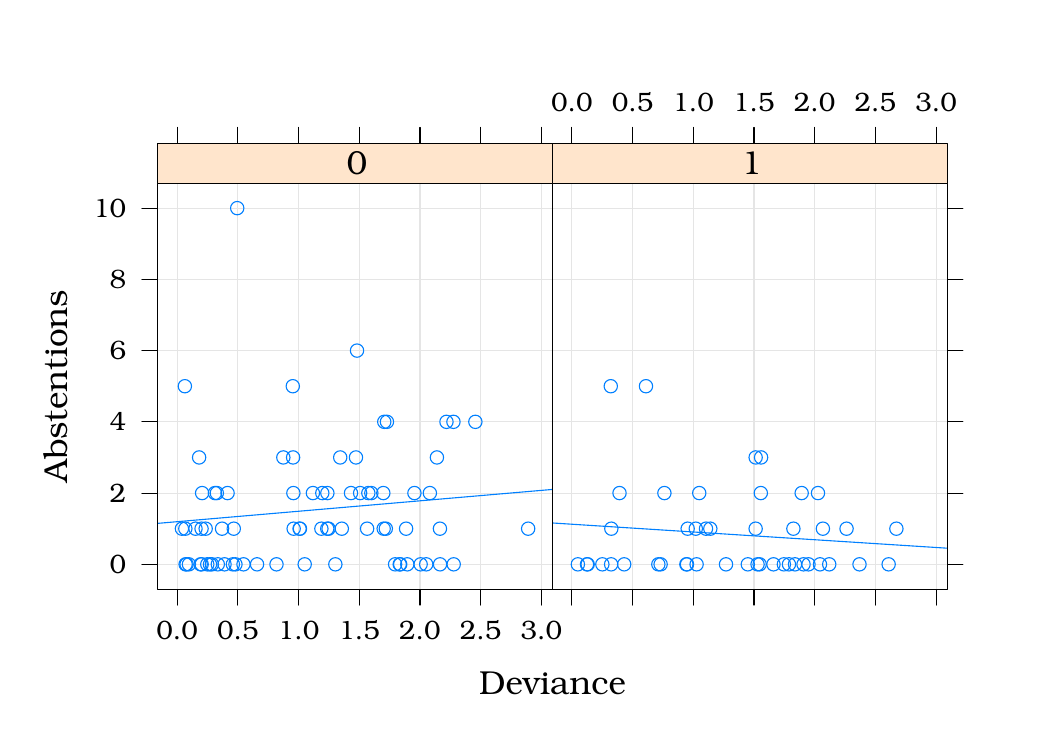
\begin{tikzpicture}[x=1pt,y=1pt]
\definecolor[named]{drawColor}{rgb}{0.00,0.00,0.00}
\definecolor[named]{fillColor}{rgb}{1.00,1.00,1.00}
\fill[color=fillColor,] (0,0) rectangle (361.35,252.94);
\begin{scope}
\path[clip] (  0.00,  0.00) rectangle (361.35,252.94);
\end{scope}
\begin{scope}
\path[clip] (  0.00,  0.00) rectangle (361.35,252.94);

\draw[fill opacity=0.00,draw opacity=0.00,] (  0.00,  0.00) rectangle (361.35,252.94);
\definecolor[named]{drawColor}{rgb}{0.00,0.00,0.00}

\node[color=drawColor,anchor=base,inner sep=0pt, outer sep=0pt, scale=  1.20] at (189.61, 12.04) {Deviance%
};
\end{scope}
\begin{scope}
\path[clip] (  0.00,  0.00) rectangle (361.35,252.94);
\definecolor[named]{drawColor}{rgb}{0.00,0.00,0.00}

\node[rotate= 90.00,color=drawColor,anchor=base,inner sep=0pt, outer sep=0pt, scale=  1.20] at ( 14.29,123.38) {Abstentions%
};
\end{scope}
\begin{scope}
\path[clip] (  0.00,  0.00) rectangle (361.35,252.94);
\end{scope}
\begin{scope}
\path[clip] (  0.00,  0.00) rectangle (361.35,252.94);
\end{scope}
\begin{scope}
\path[clip] (  0.00,  0.00) rectangle (361.35,252.94);
\end{scope}
\begin{scope}
\path[clip] ( 46.98, 50.02) rectangle (189.61,196.74);
\end{scope}
\begin{scope}
\path[clip] (  0.00,  0.00) rectangle (361.35,252.94);
\end{scope}
\begin{scope}
\path[clip] (  0.00,  0.00) rectangle (361.35,252.94);
\definecolor[named]{drawColor}{rgb}{0.00,0.00,0.00}

\draw[color=drawColor,line cap=round,line join=round,fill opacity=0.00,] ( 53.99,211.19) -- ( 53.99,216.88);

\draw[color=drawColor,line cap=round,line join=round,fill opacity=0.00,] ( 75.93,211.19) -- ( 75.93,216.88);

\draw[color=drawColor,line cap=round,line join=round,fill opacity=0.00,] ( 97.87,211.19) -- ( 97.87,216.88);

\draw[color=drawColor,line cap=round,line join=round,fill opacity=0.00,] (119.81,211.19) -- (119.81,216.88);

\draw[color=drawColor,line cap=round,line join=round,fill opacity=0.00,] (141.75,211.19) -- (141.75,216.88);

\draw[color=drawColor,line cap=round,line join=round,fill opacity=0.00,] (163.69,211.19) -- (163.69,216.88);

\draw[color=drawColor,line cap=round,line join=round,fill opacity=0.00,] (185.63,211.19) -- (185.63,216.88);
\end{scope}
\begin{scope}
\path[clip] (  0.00,  0.00) rectangle (361.35,252.94);
\end{scope}
\begin{scope}
\path[clip] (  0.00,  0.00) rectangle (361.35,252.94);
\definecolor[named]{drawColor}{rgb}{0.00,0.00,0.00}

\draw[color=drawColor,line cap=round,line join=round,fill opacity=0.00,] ( 46.98, 59.02) -- ( 41.29, 59.02);

\draw[color=drawColor,line cap=round,line join=round,fill opacity=0.00,] ( 46.98, 84.77) -- ( 41.29, 84.77);

\draw[color=drawColor,line cap=round,line join=round,fill opacity=0.00,] ( 46.98,110.51) -- ( 41.29,110.51);

\draw[color=drawColor,line cap=round,line join=round,fill opacity=0.00,] ( 46.98,136.25) -- ( 41.29,136.25);

\draw[color=drawColor,line cap=round,line join=round,fill opacity=0.00,] ( 46.98,161.99) -- ( 41.29,161.99);

\draw[color=drawColor,line cap=round,line join=round,fill opacity=0.00,] ( 46.98,187.73) -- ( 41.29,187.73);

\node[color=drawColor,anchor=base east,inner sep=0pt, outer sep=0pt, scale=  0.96] at ( 35.60, 55.72) {0%
};

\node[color=drawColor,anchor=base east,inner sep=0pt, outer sep=0pt, scale=  0.96] at ( 35.60, 81.46) {2%
};

\node[color=drawColor,anchor=base east,inner sep=0pt, outer sep=0pt, scale=  0.96] at ( 35.60,107.20) {4%
};

\node[color=drawColor,anchor=base east,inner sep=0pt, outer sep=0pt, scale=  0.96] at ( 35.60,132.94) {6%
};

\node[color=drawColor,anchor=base east,inner sep=0pt, outer sep=0pt, scale=  0.96] at ( 35.60,158.68) {8%
};

\node[color=drawColor,anchor=base east,inner sep=0pt, outer sep=0pt, scale=  0.96] at ( 35.60,184.42) {10%
};
\end{scope}
\begin{scope}
\path[clip] (  0.00,  0.00) rectangle (361.35,252.94);
\end{scope}
\begin{scope}
\path[clip] (  0.00,  0.00) rectangle (361.35,252.94);
\definecolor[named]{drawColor}{rgb}{0.00,0.00,0.00}

\draw[color=drawColor,line cap=round,line join=round,fill opacity=0.00,] ( 53.99, 50.02) -- ( 53.99, 44.32);

\draw[color=drawColor,line cap=round,line join=round,fill opacity=0.00,] ( 75.93, 50.02) -- ( 75.93, 44.32);

\draw[color=drawColor,line cap=round,line join=round,fill opacity=0.00,] ( 97.87, 50.02) -- ( 97.87, 44.32);

\draw[color=drawColor,line cap=round,line join=round,fill opacity=0.00,] (119.81, 50.02) -- (119.81, 44.32);

\draw[color=drawColor,line cap=round,line join=round,fill opacity=0.00,] (141.75, 50.02) -- (141.75, 44.32);

\draw[color=drawColor,line cap=round,line join=round,fill opacity=0.00,] (163.69, 50.02) -- (163.69, 44.32);

\draw[color=drawColor,line cap=round,line join=round,fill opacity=0.00,] (185.63, 50.02) -- (185.63, 44.32);

\node[color=drawColor,anchor=base,inner sep=0pt, outer sep=0pt, scale=  0.96] at ( 53.99, 32.02) {0.0%
};

\node[color=drawColor,anchor=base,inner sep=0pt, outer sep=0pt, scale=  0.96] at ( 75.93, 32.02) {0.5%
};

\node[color=drawColor,anchor=base,inner sep=0pt, outer sep=0pt, scale=  0.96] at ( 97.87, 32.02) {1.0%
};

\node[color=drawColor,anchor=base,inner sep=0pt, outer sep=0pt, scale=  0.96] at (119.81, 32.02) {1.5%
};

\node[color=drawColor,anchor=base,inner sep=0pt, outer sep=0pt, scale=  0.96] at (141.75, 32.02) {2.0%
};

\node[color=drawColor,anchor=base,inner sep=0pt, outer sep=0pt, scale=  0.96] at (163.69, 32.02) {2.5%
};

\node[color=drawColor,anchor=base,inner sep=0pt, outer sep=0pt, scale=  0.96] at (185.63, 32.02) {3.0%
};
\end{scope}
\begin{scope}
\path[clip] (  0.00,  0.00) rectangle (361.35,252.94);
\end{scope}
\begin{scope}
\path[clip] ( 46.98, 50.02) rectangle (189.61,196.74);
\definecolor[named]{drawColor}{rgb}{0.90,0.90,0.90}

\draw[color=drawColor,line cap=round,line join=round,fill opacity=0.00,] ( 46.98, 59.02) -- (189.61, 59.02);

\draw[color=drawColor,line cap=round,line join=round,fill opacity=0.00,] ( 46.98, 84.77) -- (189.61, 84.77);

\draw[color=drawColor,line cap=round,line join=round,fill opacity=0.00,] ( 46.98,110.51) -- (189.61,110.51);

\draw[color=drawColor,line cap=round,line join=round,fill opacity=0.00,] ( 46.98,136.25) -- (189.61,136.25);

\draw[color=drawColor,line cap=round,line join=round,fill opacity=0.00,] ( 46.98,161.99) -- (189.61,161.99);

\draw[color=drawColor,line cap=round,line join=round,fill opacity=0.00,] ( 46.98,187.73) -- (189.61,187.73);

\draw[color=drawColor,line cap=round,line join=round,fill opacity=0.00,] ( 53.99, 50.02) -- ( 53.99,196.74);

\draw[color=drawColor,line cap=round,line join=round,fill opacity=0.00,] ( 75.93, 50.02) -- ( 75.93,196.74);

\draw[color=drawColor,line cap=round,line join=round,fill opacity=0.00,] ( 97.87, 50.02) -- ( 97.87,196.74);

\draw[color=drawColor,line cap=round,line join=round,fill opacity=0.00,] (119.81, 50.02) -- (119.81,196.74);

\draw[color=drawColor,line cap=round,line join=round,fill opacity=0.00,] (141.75, 50.02) -- (141.75,196.74);

\draw[color=drawColor,line cap=round,line join=round,fill opacity=0.00,] (163.69, 50.02) -- (163.69,196.74);

\draw[color=drawColor,line cap=round,line join=round,fill opacity=0.00,] (185.63, 50.02) -- (185.63,196.74);
\definecolor[named]{drawColor}{rgb}{0.00,0.50,1.00}

\draw[color=drawColor,line cap=round,line join=round,fill opacity=0.00,] ( 71.13, 59.02) circle (  2.41);

\draw[color=drawColor,line cap=round,line join=round,fill opacity=0.00,] ( 72.23, 84.77) circle (  2.41);

\draw[color=drawColor,line cap=round,line join=round,fill opacity=0.00,] ( 75.08, 59.02) circle (  2.41);

\draw[color=drawColor,line cap=round,line join=round,fill opacity=0.00,] (148.97, 71.90) circle (  2.41);

\draw[color=drawColor,line cap=round,line join=round,fill opacity=0.00,] ( 77.98, 59.02) circle (  2.41);

\draw[color=drawColor,line cap=round,line join=round,fill opacity=0.00,] (122.66, 71.90) circle (  2.41);

\draw[color=drawColor,line cap=round,line join=round,fill opacity=0.00,] ( 98.25, 71.90) circle (  2.41);

\draw[color=drawColor,line cap=round,line join=round,fill opacity=0.00,] ( 57.07, 59.02) circle (  2.41);

\draw[color=drawColor,line cap=round,line join=round,fill opacity=0.00,] ( 61.95, 97.64) circle (  2.41);

\draw[color=drawColor,line cap=round,line join=round,fill opacity=0.00,] ( 64.90, 59.02) circle (  2.41);

\draw[color=drawColor,line cap=round,line join=round,fill opacity=0.00,] ( 95.80,123.38) circle (  2.41);

\draw[color=drawColor,line cap=round,line join=round,fill opacity=0.00,] ( 75.72,187.73) circle (  2.41);

\draw[color=drawColor,line cap=round,line join=round,fill opacity=0.00,] ( 65.88, 59.02) circle (  2.41);

\draw[color=drawColor,line cap=round,line join=round,fill opacity=0.00,] ( 68.70, 59.02) circle (  2.41);

\draw[color=drawColor,line cap=round,line join=round,fill opacity=0.00,] (120.14, 84.77) circle (  2.41);

\draw[color=drawColor,line cap=round,line join=round,fill opacity=0.00,] (134.62, 59.02) circle (  2.41);

\draw[color=drawColor,line cap=round,line join=round,fill opacity=0.00,] (132.77, 59.02) circle (  2.41);

\draw[color=drawColor,line cap=round,line join=round,fill opacity=0.00,] (134.43, 59.02) circle (  2.41);

\draw[color=drawColor,line cap=round,line join=round,fill opacity=0.00,] ( 66.56, 59.02) circle (  2.41);

\draw[color=drawColor,line cap=round,line join=round,fill opacity=0.00,] ( 82.88, 59.02) circle (  2.41);

\draw[color=drawColor,line cap=round,line join=round,fill opacity=0.00,] ( 58.27, 59.02) circle (  2.41);

\draw[color=drawColor,line cap=round,line join=round,fill opacity=0.00,] ( 64.32, 71.90) circle (  2.41);

\draw[color=drawColor,line cap=round,line join=round,fill opacity=0.00,] ( 96.11, 71.90) circle (  2.41);

\draw[color=drawColor,line cap=round,line join=round,fill opacity=0.00,] ( 70.24, 71.90) circle (  2.41);

\draw[color=drawColor,line cap=round,line join=round,fill opacity=0.00,] ( 68.35, 84.77) circle (  2.41);

\draw[color=drawColor,line cap=round,line join=round,fill opacity=0.00,] (142.00, 59.02) circle (  2.41);

\draw[color=drawColor,line cap=round,line join=round,fill opacity=0.00,] (145.33, 84.77) circle (  2.41);

\draw[color=drawColor,line cap=round,line join=round,fill opacity=0.00,] (151.33,110.51) circle (  2.41);

\draw[color=drawColor,line cap=round,line join=round,fill opacity=0.00,] (100.10, 59.02) circle (  2.41);

\draw[color=drawColor,line cap=round,line join=round,fill opacity=0.00,] ( 96.01, 84.77) circle (  2.41);

\draw[color=drawColor,line cap=round,line join=round,fill opacity=0.00,] (106.46, 84.77) circle (  2.41);

\draw[color=drawColor,line cap=round,line join=round,fill opacity=0.00,] (116.83, 84.77) circle (  2.41);

\draw[color=drawColor,line cap=round,line join=round,fill opacity=0.00,] ( 67.66, 84.77) circle (  2.41);

\draw[color=drawColor,line cap=round,line join=round,fill opacity=0.00,] (129.82,110.51) circle (  2.41);

\draw[color=drawColor,line cap=round,line join=round,fill opacity=0.00,] (161.77,110.51) circle (  2.41);

\draw[color=drawColor,line cap=round,line join=round,fill opacity=0.00,] ( 95.91, 97.64) circle (  2.41);

\draw[color=drawColor,line cap=round,line join=round,fill opacity=0.00,] ( 98.39, 71.90) circle (  2.41);

\draw[color=drawColor,line cap=round,line join=round,fill opacity=0.00,] ( 62.87, 59.02) circle (  2.41);

\draw[color=drawColor,line cap=round,line join=round,fill opacity=0.00,] (103.07, 84.77) circle (  2.41);

\draw[color=drawColor,line cap=round,line join=round,fill opacity=0.00,] (149.01, 59.02) circle (  2.41);

\draw[color=drawColor,line cap=round,line join=round,fill opacity=0.00,] (113.51, 71.90) circle (  2.41);

\draw[color=drawColor,line cap=round,line join=round,fill opacity=0.00,] ( 56.97, 71.90) circle (  2.41);

\draw[color=drawColor,line cap=round,line join=round,fill opacity=0.00,] ( 55.74, 71.90) circle (  2.41);

\draw[color=drawColor,line cap=round,line join=round,fill opacity=0.00,] (147.88, 97.64) circle (  2.41);

\draw[color=drawColor,line cap=round,line join=round,fill opacity=0.00,] (119.01,136.25) circle (  2.41);

\draw[color=drawColor,line cap=round,line join=round,fill opacity=0.00,] (129.41, 71.90) circle (  2.41);

\draw[color=drawColor,line cap=round,line join=round,fill opacity=0.00,] (136.74, 71.90) circle (  2.41);

\draw[color=drawColor,line cap=round,line join=round,fill opacity=0.00,] (137.17, 59.02) circle (  2.41);

\draw[color=drawColor,line cap=round,line join=round,fill opacity=0.00,] (144.01, 59.02) circle (  2.41);

\draw[color=drawColor,line cap=round,line join=round,fill opacity=0.00,] (153.94, 59.02) circle (  2.41);

\draw[color=drawColor,line cap=round,line join=round,fill opacity=0.00,] ( 89.91, 59.02) circle (  2.41);

\draw[color=drawColor,line cap=round,line join=round,fill opacity=0.00,] (123.10, 84.77) circle (  2.41);

\draw[color=drawColor,line cap=round,line join=round,fill opacity=0.00,] ( 56.80,123.38) circle (  2.41);

\draw[color=drawColor,line cap=round,line join=round,fill opacity=0.00,] ( 57.42, 59.02) circle (  2.41);

\draw[color=drawColor,line cap=round,line join=round,fill opacity=0.00,] (111.18, 59.02) circle (  2.41);

\draw[color=drawColor,line cap=round,line join=round,fill opacity=0.00,] ( 62.50, 59.02) circle (  2.41);

\draw[color=drawColor,line cap=round,line join=round,fill opacity=0.00,] ( 63.03, 84.77) circle (  2.41);

\draw[color=drawColor,line cap=round,line join=round,fill opacity=0.00,] ( 62.83, 71.90) circle (  2.41);

\draw[color=drawColor,line cap=round,line join=round,fill opacity=0.00,] ( 60.64, 71.90) circle (  2.41);

\draw[color=drawColor,line cap=round,line join=round,fill opacity=0.00,] (108.25, 71.90) circle (  2.41);

\draw[color=drawColor,line cap=round,line join=round,fill opacity=0.00,] ( 74.15, 59.02) circle (  2.41);

\draw[color=drawColor,line cap=round,line join=round,fill opacity=0.00,] ( 92.38, 97.64) circle (  2.41);

\draw[color=drawColor,line cap=round,line join=round,fill opacity=0.00,] (128.64, 71.90) circle (  2.41);

\draw[color=drawColor,line cap=round,line join=round,fill opacity=0.00,] (112.94, 97.64) circle (  2.41);

\draw[color=drawColor,line cap=round,line join=round,fill opacity=0.00,] (180.85, 71.90) circle (  2.41);

\draw[color=drawColor,line cap=round,line join=round,fill opacity=0.00,] (139.75, 84.77) circle (  2.41);

\draw[color=drawColor,line cap=round,line join=round,fill opacity=0.00,] (128.85,110.51) circle (  2.41);

\draw[color=drawColor,line cap=round,line join=round,fill opacity=0.00,] (128.51, 84.77) circle (  2.41);

\draw[color=drawColor,line cap=round,line join=round,fill opacity=0.00,] (124.18, 84.77) circle (  2.41);

\draw[color=drawColor,line cap=round,line join=round,fill opacity=0.00,] (153.85,110.51) circle (  2.41);

\draw[color=drawColor,line cap=round,line join=round,fill opacity=0.00,] (108.73, 71.90) circle (  2.41);

\draw[color=drawColor,line cap=round,line join=round,fill opacity=0.00,] ( 74.47, 71.90) circle (  2.41);

\draw[color=drawColor,line cap=round,line join=round,fill opacity=0.00,] (118.63, 97.64) circle (  2.41);

\draw[color=drawColor,line cap=round,line join=round,fill opacity=0.00,] (106.13, 71.90) circle (  2.41);

\draw[color=drawColor,line cap=round,line join=round,fill opacity=0.00,] (108.29, 84.77) circle (  2.41);

\draw[color=drawColor,line cap=round,line join=round,fill opacity=0.00,] (189.61, 86.08) --
	( 46.98, 73.82);
\end{scope}
\begin{scope}
\path[clip] (  0.00,  0.00) rectangle (361.35,252.94);
\end{scope}
\begin{scope}
\path[clip] (  0.00,  0.00) rectangle (361.35,252.94);
\definecolor[named]{drawColor}{rgb}{0.00,0.00,0.00}

\draw[color=drawColor,line cap=round,line join=round,fill opacity=0.00,] ( 46.98, 50.02) rectangle (189.61,196.74);
\end{scope}
\begin{scope}
\path[clip] (  0.00,  0.00) rectangle (361.35,252.94);
\end{scope}
\begin{scope}
\path[clip] (  0.00,  0.00) rectangle (361.35,252.94);
\end{scope}
\begin{scope}
\path[clip] ( 46.98,196.74) rectangle (189.61,211.19);
\definecolor[named]{drawColor}{rgb}{1.00,0.90,0.80}
\definecolor[named]{fillColor}{rgb}{1.00,0.90,0.80}

\draw[color=drawColor,line cap=round,line join=round,fill=fillColor,] ( 46.98,196.74) rectangle (189.61,211.19);
\definecolor[named]{drawColor}{rgb}{0.00,0.00,0.00}

\node[color=drawColor,anchor=base west,inner sep=0pt, outer sep=0pt, scale=  1.20] at (115.29,199.83) {0%
};
\end{scope}
\begin{scope}
\path[clip] (  0.00,  0.00) rectangle (361.35,252.94);
\end{scope}
\begin{scope}
\path[clip] (  0.00,  0.00) rectangle (361.35,252.94);
\definecolor[named]{drawColor}{rgb}{0.00,0.00,0.00}

\draw[color=drawColor,line cap=round,line join=round,fill opacity=0.00,] ( 46.98,196.74) rectangle (189.61,211.19);
\end{scope}
\begin{scope}
\path[clip] (  0.00,  0.00) rectangle (361.35,252.94);
\end{scope}
\begin{scope}
\path[clip] (  0.00,  0.00) rectangle (361.35,252.94);
\end{scope}
\begin{scope}
\path[clip] (189.61, 50.02) rectangle (332.23,196.74);
\end{scope}
\begin{scope}
\path[clip] (  0.00,  0.00) rectangle (361.35,252.94);
\end{scope}
\begin{scope}
\path[clip] (  0.00,  0.00) rectangle (361.35,252.94);
\definecolor[named]{drawColor}{rgb}{0.00,0.00,0.00}

\draw[color=drawColor,line cap=round,line join=round,fill opacity=0.00,] (196.62,211.19) -- (196.62,216.88);

\draw[color=drawColor,line cap=round,line join=round,fill opacity=0.00,] (218.56,211.19) -- (218.56,216.88);

\draw[color=drawColor,line cap=round,line join=round,fill opacity=0.00,] (240.50,211.19) -- (240.50,216.88);

\draw[color=drawColor,line cap=round,line join=round,fill opacity=0.00,] (262.44,211.19) -- (262.44,216.88);

\draw[color=drawColor,line cap=round,line join=round,fill opacity=0.00,] (284.38,211.19) -- (284.38,216.88);

\draw[color=drawColor,line cap=round,line join=round,fill opacity=0.00,] (306.32,211.19) -- (306.32,216.88);

\draw[color=drawColor,line cap=round,line join=round,fill opacity=0.00,] (328.25,211.19) -- (328.25,216.88);

\node[color=drawColor,anchor=base,inner sep=0pt, outer sep=0pt, scale=  0.96] at (196.62,222.58) {0.0%
};

\node[color=drawColor,anchor=base,inner sep=0pt, outer sep=0pt, scale=  0.96] at (218.56,222.58) {0.5%
};

\node[color=drawColor,anchor=base,inner sep=0pt, outer sep=0pt, scale=  0.96] at (240.50,222.58) {1.0%
};

\node[color=drawColor,anchor=base,inner sep=0pt, outer sep=0pt, scale=  0.96] at (262.44,222.58) {1.5%
};

\node[color=drawColor,anchor=base,inner sep=0pt, outer sep=0pt, scale=  0.96] at (284.38,222.58) {2.0%
};

\node[color=drawColor,anchor=base,inner sep=0pt, outer sep=0pt, scale=  0.96] at (306.32,222.58) {2.5%
};

\node[color=drawColor,anchor=base,inner sep=0pt, outer sep=0pt, scale=  0.96] at (328.25,222.58) {3.0%
};
\end{scope}
\begin{scope}
\path[clip] (  0.00,  0.00) rectangle (361.35,252.94);
\end{scope}
\begin{scope}
\path[clip] (  0.00,  0.00) rectangle (361.35,252.94);
\end{scope}
\begin{scope}
\path[clip] (  0.00,  0.00) rectangle (361.35,252.94);
\end{scope}
\begin{scope}
\path[clip] (  0.00,  0.00) rectangle (361.35,252.94);
\definecolor[named]{drawColor}{rgb}{0.00,0.00,0.00}

\draw[color=drawColor,line cap=round,line join=round,fill opacity=0.00,] (196.62, 50.02) -- (196.62, 44.32);

\draw[color=drawColor,line cap=round,line join=round,fill opacity=0.00,] (218.56, 50.02) -- (218.56, 44.32);

\draw[color=drawColor,line cap=round,line join=round,fill opacity=0.00,] (240.50, 50.02) -- (240.50, 44.32);

\draw[color=drawColor,line cap=round,line join=round,fill opacity=0.00,] (262.44, 50.02) -- (262.44, 44.32);

\draw[color=drawColor,line cap=round,line join=round,fill opacity=0.00,] (284.38, 50.02) -- (284.38, 44.32);

\draw[color=drawColor,line cap=round,line join=round,fill opacity=0.00,] (306.32, 50.02) -- (306.32, 44.32);

\draw[color=drawColor,line cap=round,line join=round,fill opacity=0.00,] (328.25, 50.02) -- (328.25, 44.32);

\draw[color=drawColor,line cap=round,line join=round,fill opacity=0.00,] (332.23, 59.02) -- (337.92, 59.02);

\draw[color=drawColor,line cap=round,line join=round,fill opacity=0.00,] (332.23, 84.77) -- (337.92, 84.77);

\draw[color=drawColor,line cap=round,line join=round,fill opacity=0.00,] (332.23,110.51) -- (337.92,110.51);

\draw[color=drawColor,line cap=round,line join=round,fill opacity=0.00,] (332.23,136.25) -- (337.92,136.25);

\draw[color=drawColor,line cap=round,line join=round,fill opacity=0.00,] (332.23,161.99) -- (337.92,161.99);

\draw[color=drawColor,line cap=round,line join=round,fill opacity=0.00,] (332.23,187.73) -- (337.92,187.73);
\end{scope}
\begin{scope}
\path[clip] (  0.00,  0.00) rectangle (361.35,252.94);
\end{scope}
\begin{scope}
\path[clip] (189.61, 50.02) rectangle (332.23,196.74);
\definecolor[named]{drawColor}{rgb}{0.90,0.90,0.90}

\draw[color=drawColor,line cap=round,line join=round,fill opacity=0.00,] (189.61, 59.02) -- (332.23, 59.02);

\draw[color=drawColor,line cap=round,line join=round,fill opacity=0.00,] (189.61, 84.77) -- (332.23, 84.77);

\draw[color=drawColor,line cap=round,line join=round,fill opacity=0.00,] (189.61,110.51) -- (332.23,110.51);

\draw[color=drawColor,line cap=round,line join=round,fill opacity=0.00,] (189.61,136.25) -- (332.23,136.25);

\draw[color=drawColor,line cap=round,line join=round,fill opacity=0.00,] (189.61,161.99) -- (332.23,161.99);

\draw[color=drawColor,line cap=round,line join=round,fill opacity=0.00,] (189.61,187.73) -- (332.23,187.73);

\draw[color=drawColor,line cap=round,line join=round,fill opacity=0.00,] (196.62, 50.02) -- (196.62,196.74);

\draw[color=drawColor,line cap=round,line join=round,fill opacity=0.00,] (218.56, 50.02) -- (218.56,196.74);

\draw[color=drawColor,line cap=round,line join=round,fill opacity=0.00,] (240.50, 50.02) -- (240.50,196.74);

\draw[color=drawColor,line cap=round,line join=round,fill opacity=0.00,] (262.44, 50.02) -- (262.44,196.74);

\draw[color=drawColor,line cap=round,line join=round,fill opacity=0.00,] (284.38, 50.02) -- (284.38,196.74);

\draw[color=drawColor,line cap=round,line join=round,fill opacity=0.00,] (306.32, 50.02) -- (306.32,196.74);

\draw[color=drawColor,line cap=round,line join=round,fill opacity=0.00,] (328.25, 50.02) -- (328.25,196.74);
\definecolor[named]{drawColor}{rgb}{0.00,0.50,1.00}

\draw[color=drawColor,line cap=round,line join=round,fill opacity=0.00,] (238.49, 71.90) circle (  2.41);

\draw[color=drawColor,line cap=round,line join=round,fill opacity=0.00,] (287.35, 71.90) circle (  2.41);

\draw[color=drawColor,line cap=round,line join=round,fill opacity=0.00,] (265.02, 97.64) circle (  2.41);

\draw[color=drawColor,line cap=round,line join=round,fill opacity=0.00,] (241.71, 59.02) circle (  2.41);

\draw[color=drawColor,line cap=round,line join=round,fill opacity=0.00,] (202.11, 59.02) circle (  2.41);

\draw[color=drawColor,line cap=round,line join=round,fill opacity=0.00,] (198.81, 59.02) circle (  2.41);

\draw[color=drawColor,line cap=round,line join=round,fill opacity=0.00,] (202.35, 59.02) circle (  2.41);

\draw[color=drawColor,line cap=round,line join=round,fill opacity=0.00,] (275.09, 59.02) circle (  2.41);

\draw[color=drawColor,line cap=round,line join=round,fill opacity=0.00,] (223.42,123.38) circle (  2.41);

\draw[color=drawColor,line cap=round,line join=round,fill opacity=0.00,] (210.90, 71.90) circle (  2.41);

\draw[color=drawColor,line cap=round,line join=round,fill opacity=0.00,] (242.67, 84.77) circle (  2.41);

\draw[color=drawColor,line cap=round,line join=round,fill opacity=0.00,] (295.90, 71.90) circle (  2.41);

\draw[color=drawColor,line cap=round,line join=round,fill opacity=0.00,] (246.67, 71.90) circle (  2.41);

\draw[color=drawColor,line cap=round,line join=round,fill opacity=0.00,] (311.11, 59.02) circle (  2.41);

\draw[color=drawColor,line cap=round,line join=round,fill opacity=0.00,] (285.58, 84.77) circle (  2.41);

\draw[color=drawColor,line cap=round,line join=round,fill opacity=0.00,] (313.91, 71.90) circle (  2.41);

\draw[color=drawColor,line cap=round,line join=round,fill opacity=0.00,] (280.35, 59.02) circle (  2.41);

\draw[color=drawColor,line cap=round,line join=round,fill opacity=0.00,] (282.15, 59.02) circle (  2.41);

\draw[color=drawColor,line cap=round,line join=round,fill opacity=0.00,] (264.92, 84.77) circle (  2.41);

\draw[color=drawColor,line cap=round,line join=round,fill opacity=0.00,] (238.02, 59.02) circle (  2.41);

\draw[color=drawColor,line cap=round,line join=round,fill opacity=0.00,] (263.74, 59.02) circle (  2.41);

\draw[color=drawColor,line cap=round,line join=round,fill opacity=0.00,] (245.11, 71.90) circle (  2.41);

\draw[color=drawColor,line cap=round,line join=round,fill opacity=0.00,] (238.24, 59.02) circle (  2.41);

\draw[color=drawColor,line cap=round,line join=round,fill opacity=0.00,] (263.05, 97.64) circle (  2.41);

\draw[color=drawColor,line cap=round,line join=round,fill opacity=0.00,] (264.49, 59.02) circle (  2.41);

\draw[color=drawColor,line cap=round,line join=round,fill opacity=0.00,] (263.05, 71.90) circle (  2.41);

\draw[color=drawColor,line cap=round,line join=round,fill opacity=0.00,] (269.49, 59.02) circle (  2.41);

\draw[color=drawColor,line cap=round,line join=round,fill opacity=0.00,] (210.70,123.38) circle (  2.41);

\draw[color=drawColor,line cap=round,line join=round,fill opacity=0.00,] (289.64, 59.02) circle (  2.41);

\draw[color=drawColor,line cap=round,line join=round,fill opacity=0.00,] (227.89, 59.02) circle (  2.41);

\draw[color=drawColor,line cap=round,line join=round,fill opacity=0.00,] (230.08, 84.77) circle (  2.41);

\draw[color=drawColor,line cap=round,line join=round,fill opacity=0.00,] (279.68, 84.77) circle (  2.41);

\draw[color=drawColor,line cap=round,line join=round,fill opacity=0.00,] (276.69, 71.90) circle (  2.41);

\draw[color=drawColor,line cap=round,line join=round,fill opacity=0.00,] (300.58, 59.02) circle (  2.41);

\draw[color=drawColor,line cap=round,line join=round,fill opacity=0.00,] (286.30, 59.02) circle (  2.41);

\draw[color=drawColor,line cap=round,line join=round,fill opacity=0.00,] (207.66, 59.02) circle (  2.41);

\draw[color=drawColor,line cap=round,line join=round,fill opacity=0.00,] (241.42, 71.90) circle (  2.41);

\draw[color=drawColor,line cap=round,line join=round,fill opacity=0.00,] (210.83, 59.02) circle (  2.41);

\draw[color=drawColor,line cap=round,line join=round,fill opacity=0.00,] (213.86, 84.77) circle (  2.41);

\draw[color=drawColor,line cap=round,line join=round,fill opacity=0.00,] (260.22, 59.02) circle (  2.41);

\draw[color=drawColor,line cap=round,line join=round,fill opacity=0.00,] (252.34, 59.02) circle (  2.41);

\draw[color=drawColor,line cap=round,line join=round,fill opacity=0.00,] (215.55, 59.02) circle (  2.41);

\draw[color=drawColor,line cap=round,line join=round,fill opacity=0.00,] (228.71, 59.02) circle (  2.41);

\draw[color=drawColor,line cap=round,line join=round,fill opacity=0.00,] (277.27, 59.02) circle (  2.41);

\draw[color=drawColor,line cap=round,line join=round,fill opacity=0.00,] (273.25, 59.02) circle (  2.41);

\draw[color=drawColor,line cap=round,line join=round,fill opacity=0.00,] (332.23, 64.85) --
	(189.61, 73.96);
\end{scope}
\begin{scope}
\path[clip] (  0.00,  0.00) rectangle (361.35,252.94);
\end{scope}
\begin{scope}
\path[clip] (  0.00,  0.00) rectangle (361.35,252.94);
\definecolor[named]{drawColor}{rgb}{0.00,0.00,0.00}

\draw[color=drawColor,line cap=round,line join=round,fill opacity=0.00,] (189.61, 50.02) rectangle (332.23,196.74);
\end{scope}
\begin{scope}
\path[clip] (  0.00,  0.00) rectangle (361.35,252.94);
\end{scope}
\begin{scope}
\path[clip] (  0.00,  0.00) rectangle (361.35,252.94);
\end{scope}
\begin{scope}
\path[clip] (189.61,196.74) rectangle (332.23,211.19);
\definecolor[named]{drawColor}{rgb}{1.00,0.90,0.80}
\definecolor[named]{fillColor}{rgb}{1.00,0.90,0.80}

\draw[color=drawColor,line cap=round,line join=round,fill=fillColor,] (189.61,196.74) rectangle (332.23,211.19);
\definecolor[named]{drawColor}{rgb}{0.00,0.00,0.00}

\node[color=drawColor,anchor=base west,inner sep=0pt, outer sep=0pt, scale=  1.20] at (257.92,199.83) {1%
};
\end{scope}
\begin{scope}
\path[clip] (  0.00,  0.00) rectangle (361.35,252.94);
\end{scope}
\begin{scope}
\path[clip] (  0.00,  0.00) rectangle (361.35,252.94);
\definecolor[named]{drawColor}{rgb}{0.00,0.00,0.00}

\draw[color=drawColor,line cap=round,line join=round,fill opacity=0.00,] (189.61,196.74) rectangle (332.23,211.19);
\end{scope}
\begin{scope}
\path[clip] (  0.00,  0.00) rectangle (361.35,252.94);
\end{scope}
\begin{scope}
\path[clip] (  0.00,  0.00) rectangle (361.35,252.94);
\end{scope}
\begin{scope}
\path[clip] (  0.00,  0.00) rectangle (361.35,252.94);
\end{scope}
\begin{scope}
\path[clip] (  0.00,  0.00) rectangle (361.35,252.94);
\end{scope}
\end{tikzpicture}
}}\quad
\scalebox{.6}{\subfloat[][]{% Created by tikzDevice version 0.6.1 on 2011-08-03 09:50:59
% !TEX encoding = UTF-8 Unicode
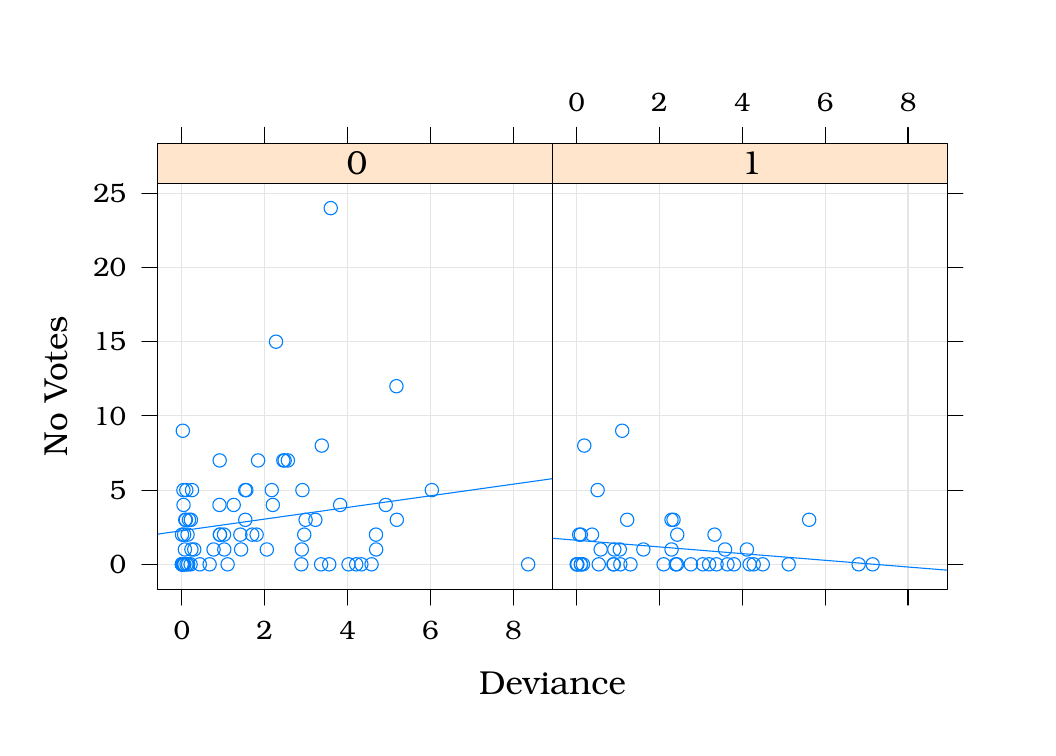
\begin{tikzpicture}[x=1pt,y=1pt]
\definecolor[named]{drawColor}{rgb}{0.00,0.00,0.00}
\definecolor[named]{fillColor}{rgb}{1.00,1.00,1.00}
\fill[color=fillColor,] (0,0) rectangle (361.35,252.94);
\begin{scope}
\path[clip] (  0.00,  0.00) rectangle (361.35,252.94);
\definecolor[named]{fillColor}{rgb}{0.00,0.00,0.00}
\end{scope}
\begin{scope}
\path[clip] (  0.00,  0.00) rectangle (361.35,252.94);
\definecolor[named]{fillColor}{rgb}{0.00,0.00,0.00}

\draw[fill opacity=0.00,draw opacity=0.00,] (  0.00,  0.00) rectangle (361.35,252.94);
\definecolor[named]{drawColor}{rgb}{0.00,0.00,0.00}

\node[color=drawColor,anchor=base,inner sep=0pt, outer sep=0pt, scale=  1.20] at (189.61, 12.04) {Deviance%
};
\end{scope}
\begin{scope}
\path[clip] (  0.00,  0.00) rectangle (361.35,252.94);
\definecolor[named]{fillColor}{rgb}{0.00,0.00,0.00}
\definecolor[named]{drawColor}{rgb}{0.00,0.00,0.00}

\node[rotate= 90.00,color=drawColor,anchor=base,inner sep=0pt, outer sep=0pt, scale=  1.20] at ( 14.29,123.38) {No Votes%
};
\end{scope}
\begin{scope}
\path[clip] (  0.00,  0.00) rectangle (361.35,252.94);
\definecolor[named]{fillColor}{rgb}{0.00,0.00,0.00}
\end{scope}
\begin{scope}
\path[clip] (  0.00,  0.00) rectangle (361.35,252.94);
\definecolor[named]{fillColor}{rgb}{0.00,0.00,0.00}
\end{scope}
\begin{scope}
\path[clip] (  0.00,  0.00) rectangle (361.35,252.94);
\definecolor[named]{fillColor}{rgb}{0.00,0.00,0.00}
\end{scope}
\begin{scope}
\path[clip] ( 46.98, 50.02) rectangle (189.61,196.74);
\definecolor[named]{fillColor}{rgb}{0.00,0.00,0.00}
\end{scope}
\begin{scope}
\path[clip] (  0.00,  0.00) rectangle (361.35,252.94);
\definecolor[named]{fillColor}{rgb}{0.00,0.00,0.00}
\end{scope}
\begin{scope}
\path[clip] (  0.00,  0.00) rectangle (361.35,252.94);
\definecolor[named]{fillColor}{rgb}{0.00,0.00,0.00}
\definecolor[named]{drawColor}{rgb}{0.00,0.00,0.00}

\draw[color=drawColor,line cap=round,line join=round,fill opacity=0.00,] ( 55.71,211.19) -- ( 55.71,216.88);

\draw[color=drawColor,line cap=round,line join=round,fill opacity=0.00,] ( 85.66,211.19) -- ( 85.66,216.88);

\draw[color=drawColor,line cap=round,line join=round,fill opacity=0.00,] (115.60,211.19) -- (115.60,216.88);

\draw[color=drawColor,line cap=round,line join=round,fill opacity=0.00,] (145.54,211.19) -- (145.54,216.88);

\draw[color=drawColor,line cap=round,line join=round,fill opacity=0.00,] (175.48,211.19) -- (175.48,216.88);
\end{scope}
\begin{scope}
\path[clip] (  0.00,  0.00) rectangle (361.35,252.94);
\definecolor[named]{fillColor}{rgb}{0.00,0.00,0.00}
\end{scope}
\begin{scope}
\path[clip] (  0.00,  0.00) rectangle (361.35,252.94);
\definecolor[named]{fillColor}{rgb}{0.00,0.00,0.00}
\definecolor[named]{drawColor}{rgb}{0.00,0.00,0.00}

\draw[color=drawColor,line cap=round,line join=round,fill opacity=0.00,] ( 46.98, 59.02) -- ( 41.29, 59.02);

\draw[color=drawColor,line cap=round,line join=round,fill opacity=0.00,] ( 46.98, 85.84) -- ( 41.29, 85.84);

\draw[color=drawColor,line cap=round,line join=round,fill opacity=0.00,] ( 46.98,112.65) -- ( 41.29,112.65);

\draw[color=drawColor,line cap=round,line join=round,fill opacity=0.00,] ( 46.98,139.47) -- ( 41.29,139.47);

\draw[color=drawColor,line cap=round,line join=round,fill opacity=0.00,] ( 46.98,166.28) -- ( 41.29,166.28);

\draw[color=drawColor,line cap=round,line join=round,fill opacity=0.00,] ( 46.98,193.09) -- ( 41.29,193.09);

\node[color=drawColor,anchor=base east,inner sep=0pt, outer sep=0pt, scale=  0.96] at ( 35.60, 55.72) {0%
};

\node[color=drawColor,anchor=base east,inner sep=0pt, outer sep=0pt, scale=  0.96] at ( 35.60, 82.53) {5%
};

\node[color=drawColor,anchor=base east,inner sep=0pt, outer sep=0pt, scale=  0.96] at ( 35.60,109.35) {10%
};

\node[color=drawColor,anchor=base east,inner sep=0pt, outer sep=0pt, scale=  0.96] at ( 35.60,136.16) {15%
};

\node[color=drawColor,anchor=base east,inner sep=0pt, outer sep=0pt, scale=  0.96] at ( 35.60,162.97) {20%
};

\node[color=drawColor,anchor=base east,inner sep=0pt, outer sep=0pt, scale=  0.96] at ( 35.60,189.79) {25%
};
\end{scope}
\begin{scope}
\path[clip] (  0.00,  0.00) rectangle (361.35,252.94);
\definecolor[named]{fillColor}{rgb}{0.00,0.00,0.00}
\end{scope}
\begin{scope}
\path[clip] (  0.00,  0.00) rectangle (361.35,252.94);
\definecolor[named]{fillColor}{rgb}{0.00,0.00,0.00}
\definecolor[named]{drawColor}{rgb}{0.00,0.00,0.00}

\draw[color=drawColor,line cap=round,line join=round,fill opacity=0.00,] ( 55.71, 50.02) -- ( 55.71, 44.32);

\draw[color=drawColor,line cap=round,line join=round,fill opacity=0.00,] ( 85.66, 50.02) -- ( 85.66, 44.32);

\draw[color=drawColor,line cap=round,line join=round,fill opacity=0.00,] (115.60, 50.02) -- (115.60, 44.32);

\draw[color=drawColor,line cap=round,line join=round,fill opacity=0.00,] (145.54, 50.02) -- (145.54, 44.32);

\draw[color=drawColor,line cap=round,line join=round,fill opacity=0.00,] (175.48, 50.02) -- (175.48, 44.32);

\node[color=drawColor,anchor=base,inner sep=0pt, outer sep=0pt, scale=  0.96] at ( 55.71, 32.02) {0%
};

\node[color=drawColor,anchor=base,inner sep=0pt, outer sep=0pt, scale=  0.96] at ( 85.66, 32.02) {2%
};

\node[color=drawColor,anchor=base,inner sep=0pt, outer sep=0pt, scale=  0.96] at (115.60, 32.02) {4%
};

\node[color=drawColor,anchor=base,inner sep=0pt, outer sep=0pt, scale=  0.96] at (145.54, 32.02) {6%
};

\node[color=drawColor,anchor=base,inner sep=0pt, outer sep=0pt, scale=  0.96] at (175.48, 32.02) {8%
};
\end{scope}
\begin{scope}
\path[clip] (  0.00,  0.00) rectangle (361.35,252.94);
\definecolor[named]{fillColor}{rgb}{0.00,0.00,0.00}
\end{scope}
\begin{scope}
\path[clip] ( 46.98, 50.02) rectangle (189.61,196.74);
\definecolor[named]{fillColor}{rgb}{0.00,0.00,0.00}
\definecolor[named]{drawColor}{rgb}{0.90,0.90,0.90}

\draw[color=drawColor,line cap=round,line join=round,fill opacity=0.00,] ( 46.98, 59.02) -- (189.61, 59.02);

\draw[color=drawColor,line cap=round,line join=round,fill opacity=0.00,] ( 46.98, 85.84) -- (189.61, 85.84);

\draw[color=drawColor,line cap=round,line join=round,fill opacity=0.00,] ( 46.98,112.65) -- (189.61,112.65);

\draw[color=drawColor,line cap=round,line join=round,fill opacity=0.00,] ( 46.98,139.47) -- (189.61,139.47);

\draw[color=drawColor,line cap=round,line join=round,fill opacity=0.00,] ( 46.98,166.28) -- (189.61,166.28);

\draw[color=drawColor,line cap=round,line join=round,fill opacity=0.00,] ( 46.98,193.09) -- (189.61,193.09);

\draw[color=drawColor,line cap=round,line join=round,fill opacity=0.00,] ( 55.71, 50.02) -- ( 55.71,196.74);

\draw[color=drawColor,line cap=round,line join=round,fill opacity=0.00,] ( 85.66, 50.02) -- ( 85.66,196.74);

\draw[color=drawColor,line cap=round,line join=round,fill opacity=0.00,] (115.60, 50.02) -- (115.60,196.74);

\draw[color=drawColor,line cap=round,line join=round,fill opacity=0.00,] (145.54, 50.02) -- (145.54,196.74);

\draw[color=drawColor,line cap=round,line join=round,fill opacity=0.00,] (175.48, 50.02) -- (175.48,196.74);
\definecolor[named]{drawColor}{rgb}{0.00,0.50,1.00}

\draw[color=drawColor,line cap=round,line join=round,fill opacity=0.00,] ( 58.00, 59.02) circle (  2.41);

\draw[color=drawColor,line cap=round,line join=round,fill opacity=0.00,] ( 58.30, 75.11) circle (  2.41);

\draw[color=drawColor,line cap=round,line join=round,fill opacity=0.00,] ( 59.17, 64.39) circle (  2.41);

\draw[color=drawColor,line cap=round,line join=round,fill opacity=0.00,] (125.86, 69.75) circle (  2.41);

\draw[color=drawColor,line cap=round,line join=round,fill opacity=0.00,] ( 60.19, 64.39) circle (  2.41);

\draw[color=drawColor,line cap=round,line join=round,fill opacity=0.00,] ( 92.38, 96.56) circle (  2.41);

\draw[color=drawColor,line cap=round,line join=round,fill opacity=0.00,] ( 70.94, 69.75) circle (  2.41);

\draw[color=drawColor,line cap=round,line join=round,fill opacity=0.00,] ( 55.79, 59.02) circle (  2.41);

\draw[color=drawColor,line cap=round,line join=round,fill opacity=0.00,] ( 56.21, 59.02) circle (  2.41);

\draw[color=drawColor,line cap=round,line join=round,fill opacity=0.00,] ( 56.64, 59.02) circle (  2.41);

\draw[color=drawColor,line cap=round,line join=round,fill opacity=0.00,] ( 69.31, 80.48) circle (  2.41);

\draw[color=drawColor,line cap=round,line join=round,fill opacity=0.00,] ( 59.38, 85.84) circle (  2.41);

\draw[color=drawColor,line cap=round,line join=round,fill opacity=0.00,] ( 56.81, 64.39) circle (  2.41);

\draw[color=drawColor,line cap=round,line join=round,fill opacity=0.00,] ( 57.40, 59.02) circle (  2.41);

\draw[color=drawColor,line cap=round,line join=round,fill opacity=0.00,] ( 89.74,139.47) circle (  2.41);

\draw[color=drawColor,line cap=round,line join=round,fill opacity=0.00,] (106.27,101.93) circle (  2.41);

\draw[color=drawColor,line cap=round,line join=round,fill opacity=0.00,] (103.97, 75.11) circle (  2.41);

\draw[color=drawColor,line cap=round,line join=round,fill opacity=0.00,] (106.03, 59.02) circle (  2.41);

\draw[color=drawColor,line cap=round,line join=round,fill opacity=0.00,] ( 56.94, 75.11) circle (  2.41);

\draw[color=drawColor,line cap=round,line join=round,fill opacity=0.00,] ( 62.20, 59.02) circle (  2.41);

\draw[color=drawColor,line cap=round,line join=round,fill opacity=0.00,] ( 55.86, 59.02) circle (  2.41);

\draw[color=drawColor,line cap=round,line join=round,fill opacity=0.00,] ( 56.54, 69.75) circle (  2.41);

\draw[color=drawColor,line cap=round,line join=round,fill opacity=0.00,] ( 69.51, 69.75) circle (  2.41);

\draw[color=drawColor,line cap=round,line join=round,fill opacity=0.00,] ( 57.77, 69.75) circle (  2.41);

\draw[color=drawColor,line cap=round,line join=round,fill opacity=0.00,] ( 57.32, 85.84) circle (  2.41);

\draw[color=drawColor,line cap=round,line join=round,fill opacity=0.00,] (115.94, 59.02) circle (  2.41);

\draw[color=drawColor,line cap=round,line join=round,fill opacity=0.00,] (120.58, 59.02) circle (  2.41);

\draw[color=drawColor,line cap=round,line join=round,fill opacity=0.00,] (129.39, 80.48) circle (  2.41);

\draw[color=drawColor,line cap=round,line join=round,fill opacity=0.00,] ( 72.25, 59.02) circle (  2.41);

\draw[color=drawColor,line cap=round,line join=round,fill opacity=0.00,] ( 69.44, 69.75) circle (  2.41);

\draw[color=drawColor,line cap=round,line join=round,fill opacity=0.00,] ( 77.12, 64.39) circle (  2.41);

\draw[color=drawColor,line cap=round,line join=round,fill opacity=0.00,] ( 86.42, 64.39) circle (  2.41);

\draw[color=drawColor,line cap=round,line join=round,fill opacity=0.00,] ( 57.17, 75.11) circle (  2.41);

\draw[color=drawColor,line cap=round,line join=round,fill opacity=0.00,] (100.43, 75.11) circle (  2.41);

\draw[color=drawColor,line cap=round,line join=round,fill opacity=0.00,] (146.05, 85.84) circle (  2.41);

\draw[color=drawColor,line cap=round,line join=round,fill opacity=0.00,] ( 69.38, 96.56) circle (  2.41);

\draw[color=drawColor,line cap=round,line join=round,fill opacity=0.00,] ( 71.04, 64.39) circle (  2.41);

\draw[color=drawColor,line cap=round,line join=round,fill opacity=0.00,] ( 56.33, 59.02) circle (  2.41);

\draw[color=drawColor,line cap=round,line join=round,fill opacity=0.00,] ( 74.44, 80.48) circle (  2.41);

\draw[color=drawColor,line cap=round,line join=round,fill opacity=0.00,] (125.92, 64.39) circle (  2.41);

\draw[color=drawColor,line cap=round,line join=round,fill opacity=0.00,] ( 83.26, 96.56) circle (  2.41);

\draw[color=drawColor,line cap=round,line join=round,fill opacity=0.00,] ( 55.78, 59.02) circle (  2.41);

\draw[color=drawColor,line cap=round,line join=round,fill opacity=0.00,] ( 55.74, 59.02) circle (  2.41);

\draw[color=drawColor,line cap=round,line join=round,fill opacity=0.00,] (124.26, 59.02) circle (  2.41);

\draw[color=drawColor,line cap=round,line join=round,fill opacity=0.00,] ( 88.58, 80.48) circle (  2.41);

\draw[color=drawColor,line cap=round,line join=round,fill opacity=0.00,] ( 99.94, 69.75) circle (  2.41);

\draw[color=drawColor,line cap=round,line join=round,fill opacity=0.00,] (108.96, 59.02) circle (  2.41);

\draw[color=drawColor,line cap=round,line join=round,fill opacity=0.00,] (109.51,187.73) circle (  2.41);

\draw[color=drawColor,line cap=round,line join=round,fill opacity=0.00,] (118.72, 59.02) circle (  2.41);

\draw[color=drawColor,line cap=round,line join=round,fill opacity=0.00,] (133.39, 75.11) circle (  2.41);

\draw[color=drawColor,line cap=round,line join=round,fill opacity=0.00,] ( 65.74, 59.02) circle (  2.41);

\draw[color=drawColor,line cap=round,line join=round,fill opacity=0.00,] ( 92.85, 96.56) circle (  2.41);

\draw[color=drawColor,line cap=round,line join=round,fill opacity=0.00,] ( 55.77, 69.75) circle (  2.41);

\draw[color=drawColor,line cap=round,line join=round,fill opacity=0.00,] ( 55.80, 59.02) circle (  2.41);

\draw[color=drawColor,line cap=round,line join=round,fill opacity=0.00,] ( 81.15, 69.75) circle (  2.41);

\draw[color=drawColor,line cap=round,line join=round,fill opacity=0.00,] ( 56.28, 85.84) circle (  2.41);

\draw[color=drawColor,line cap=round,line join=round,fill opacity=0.00,] ( 56.35, 59.02) circle (  2.41);

\draw[color=drawColor,line cap=round,line join=round,fill opacity=0.00,] ( 56.32, 80.48) circle (  2.41);

\draw[color=drawColor,line cap=round,line join=round,fill opacity=0.00,] ( 56.06,107.29) circle (  2.41);

\draw[color=drawColor,line cap=round,line join=round,fill opacity=0.00,] ( 78.61, 85.84) circle (  2.41);

\draw[color=drawColor,line cap=round,line join=round,fill opacity=0.00,] ( 58.87, 59.02) circle (  2.41);

\draw[color=drawColor,line cap=round,line join=round,fill opacity=0.00,] ( 67.17, 64.39) circle (  2.41);

\draw[color=drawColor,line cap=round,line join=round,fill opacity=0.00,] ( 99.05, 64.39) circle (  2.41);

\draw[color=drawColor,line cap=round,line join=round,fill opacity=0.00,] ( 82.73, 69.75) circle (  2.41);

\draw[color=drawColor,line cap=round,line join=round,fill opacity=0.00,] (180.85, 59.02) circle (  2.41);

\draw[color=drawColor,line cap=round,line join=round,fill opacity=0.00,] (112.90, 80.48) circle (  2.41);

\draw[color=drawColor,line cap=round,line join=round,fill opacity=0.00,] ( 99.28, 85.84) circle (  2.41);

\draw[color=drawColor,line cap=round,line join=round,fill opacity=0.00,] ( 98.89, 59.02) circle (  2.41);

\draw[color=drawColor,line cap=round,line join=round,fill opacity=0.00,] ( 94.02, 96.56) circle (  2.41);

\draw[color=drawColor,line cap=round,line join=round,fill opacity=0.00,] (133.25,123.38) circle (  2.41);

\draw[color=drawColor,line cap=round,line join=round,fill opacity=0.00,] ( 79.01, 85.84) circle (  2.41);

\draw[color=drawColor,line cap=round,line join=round,fill opacity=0.00,] ( 58.98, 75.11) circle (  2.41);

\draw[color=drawColor,line cap=round,line join=round,fill opacity=0.00,] ( 88.20, 85.84) circle (  2.41);

\draw[color=drawColor,line cap=round,line join=round,fill opacity=0.00,] ( 76.85, 69.75) circle (  2.41);

\draw[color=drawColor,line cap=round,line join=round,fill opacity=0.00,] ( 78.64, 75.11) circle (  2.41);

\draw[color=drawColor,line cap=round,line join=round,fill opacity=0.00,] (189.61, 89.97) --
	( 46.98, 69.94);
\end{scope}
\begin{scope}
\path[clip] (  0.00,  0.00) rectangle (361.35,252.94);
\definecolor[named]{fillColor}{rgb}{0.00,0.00,0.00}
\end{scope}
\begin{scope}
\path[clip] (  0.00,  0.00) rectangle (361.35,252.94);
\definecolor[named]{fillColor}{rgb}{0.00,0.00,0.00}
\definecolor[named]{drawColor}{rgb}{0.00,0.00,0.00}

\draw[color=drawColor,line cap=round,line join=round,fill opacity=0.00,] ( 46.98, 50.02) rectangle (189.61,196.74);
\end{scope}
\begin{scope}
\path[clip] (  0.00,  0.00) rectangle (361.35,252.94);
\definecolor[named]{fillColor}{rgb}{0.00,0.00,0.00}
\end{scope}
\begin{scope}
\path[clip] (  0.00,  0.00) rectangle (361.35,252.94);
\definecolor[named]{fillColor}{rgb}{0.00,0.00,0.00}
\end{scope}
\begin{scope}
\path[clip] ( 46.98,196.74) rectangle (189.61,211.19);
\definecolor[named]{fillColor}{rgb}{0.00,0.00,0.00}
\definecolor[named]{drawColor}{rgb}{1.00,0.90,0.80}
\definecolor[named]{fillColor}{rgb}{1.00,0.90,0.80}

\draw[color=drawColor,line cap=round,line join=round,fill=fillColor,] ( 46.98,196.74) rectangle (189.61,211.19);
\definecolor[named]{drawColor}{rgb}{0.00,0.00,0.00}

\node[color=drawColor,anchor=base west,inner sep=0pt, outer sep=0pt, scale=  1.20] at (115.29,199.83) {0%
};
\end{scope}
\begin{scope}
\path[clip] (  0.00,  0.00) rectangle (361.35,252.94);
\definecolor[named]{fillColor}{rgb}{0.00,0.00,0.00}
\end{scope}
\begin{scope}
\path[clip] (  0.00,  0.00) rectangle (361.35,252.94);
\definecolor[named]{fillColor}{rgb}{0.00,0.00,0.00}
\definecolor[named]{drawColor}{rgb}{0.00,0.00,0.00}

\draw[color=drawColor,line cap=round,line join=round,fill opacity=0.00,] ( 46.98,196.74) rectangle (189.61,211.19);
\end{scope}
\begin{scope}
\path[clip] (  0.00,  0.00) rectangle (361.35,252.94);
\definecolor[named]{fillColor}{rgb}{0.00,0.00,0.00}
\end{scope}
\begin{scope}
\path[clip] (  0.00,  0.00) rectangle (361.35,252.94);
\definecolor[named]{fillColor}{rgb}{0.00,0.00,0.00}
\end{scope}
\begin{scope}
\path[clip] (189.61, 50.02) rectangle (332.23,196.74);
\definecolor[named]{fillColor}{rgb}{0.00,0.00,0.00}
\end{scope}
\begin{scope}
\path[clip] (  0.00,  0.00) rectangle (361.35,252.94);
\definecolor[named]{fillColor}{rgb}{0.00,0.00,0.00}
\end{scope}
\begin{scope}
\path[clip] (  0.00,  0.00) rectangle (361.35,252.94);
\definecolor[named]{fillColor}{rgb}{0.00,0.00,0.00}
\definecolor[named]{drawColor}{rgb}{0.00,0.00,0.00}

\draw[color=drawColor,line cap=round,line join=round,fill opacity=0.00,] (198.34,211.19) -- (198.34,216.88);

\draw[color=drawColor,line cap=round,line join=round,fill opacity=0.00,] (228.28,211.19) -- (228.28,216.88);

\draw[color=drawColor,line cap=round,line join=round,fill opacity=0.00,] (258.23,211.19) -- (258.23,216.88);

\draw[color=drawColor,line cap=round,line join=round,fill opacity=0.00,] (288.17,211.19) -- (288.17,216.88);

\draw[color=drawColor,line cap=round,line join=round,fill opacity=0.00,] (318.11,211.19) -- (318.11,216.88);

\node[color=drawColor,anchor=base,inner sep=0pt, outer sep=0pt, scale=  0.96] at (198.34,222.58) {0%
};

\node[color=drawColor,anchor=base,inner sep=0pt, outer sep=0pt, scale=  0.96] at (228.28,222.58) {2%
};

\node[color=drawColor,anchor=base,inner sep=0pt, outer sep=0pt, scale=  0.96] at (258.23,222.58) {4%
};

\node[color=drawColor,anchor=base,inner sep=0pt, outer sep=0pt, scale=  0.96] at (288.17,222.58) {6%
};

\node[color=drawColor,anchor=base,inner sep=0pt, outer sep=0pt, scale=  0.96] at (318.11,222.58) {8%
};
\end{scope}
\begin{scope}
\path[clip] (  0.00,  0.00) rectangle (361.35,252.94);
\definecolor[named]{fillColor}{rgb}{0.00,0.00,0.00}
\end{scope}
\begin{scope}
\path[clip] (  0.00,  0.00) rectangle (361.35,252.94);
\definecolor[named]{fillColor}{rgb}{0.00,0.00,0.00}
\end{scope}
\begin{scope}
\path[clip] (  0.00,  0.00) rectangle (361.35,252.94);
\definecolor[named]{fillColor}{rgb}{0.00,0.00,0.00}
\end{scope}
\begin{scope}
\path[clip] (  0.00,  0.00) rectangle (361.35,252.94);
\definecolor[named]{fillColor}{rgb}{0.00,0.00,0.00}
\definecolor[named]{drawColor}{rgb}{0.00,0.00,0.00}

\draw[color=drawColor,line cap=round,line join=round,fill opacity=0.00,] (198.34, 50.02) -- (198.34, 44.32);

\draw[color=drawColor,line cap=round,line join=round,fill opacity=0.00,] (228.28, 50.02) -- (228.28, 44.32);

\draw[color=drawColor,line cap=round,line join=round,fill opacity=0.00,] (258.23, 50.02) -- (258.23, 44.32);

\draw[color=drawColor,line cap=round,line join=round,fill opacity=0.00,] (288.17, 50.02) -- (288.17, 44.32);

\draw[color=drawColor,line cap=round,line join=round,fill opacity=0.00,] (318.11, 50.02) -- (318.11, 44.32);

\draw[color=drawColor,line cap=round,line join=round,fill opacity=0.00,] (332.23, 59.02) -- (337.92, 59.02);

\draw[color=drawColor,line cap=round,line join=round,fill opacity=0.00,] (332.23, 85.84) -- (337.92, 85.84);

\draw[color=drawColor,line cap=round,line join=round,fill opacity=0.00,] (332.23,112.65) -- (337.92,112.65);

\draw[color=drawColor,line cap=round,line join=round,fill opacity=0.00,] (332.23,139.47) -- (337.92,139.47);

\draw[color=drawColor,line cap=round,line join=round,fill opacity=0.00,] (332.23,166.28) -- (337.92,166.28);

\draw[color=drawColor,line cap=round,line join=round,fill opacity=0.00,] (332.23,193.09) -- (337.92,193.09);
\end{scope}
\begin{scope}
\path[clip] (  0.00,  0.00) rectangle (361.35,252.94);
\definecolor[named]{fillColor}{rgb}{0.00,0.00,0.00}
\end{scope}
\begin{scope}
\path[clip] (189.61, 50.02) rectangle (332.23,196.74);
\definecolor[named]{fillColor}{rgb}{0.00,0.00,0.00}
\definecolor[named]{drawColor}{rgb}{0.90,0.90,0.90}

\draw[color=drawColor,line cap=round,line join=round,fill opacity=0.00,] (189.61, 59.02) -- (332.23, 59.02);

\draw[color=drawColor,line cap=round,line join=round,fill opacity=0.00,] (189.61, 85.84) -- (332.23, 85.84);

\draw[color=drawColor,line cap=round,line join=round,fill opacity=0.00,] (189.61,112.65) -- (332.23,112.65);

\draw[color=drawColor,line cap=round,line join=round,fill opacity=0.00,] (189.61,139.47) -- (332.23,139.47);

\draw[color=drawColor,line cap=round,line join=round,fill opacity=0.00,] (189.61,166.28) -- (332.23,166.28);

\draw[color=drawColor,line cap=round,line join=round,fill opacity=0.00,] (189.61,193.09) -- (332.23,193.09);

\draw[color=drawColor,line cap=round,line join=round,fill opacity=0.00,] (198.34, 50.02) -- (198.34,196.74);

\draw[color=drawColor,line cap=round,line join=round,fill opacity=0.00,] (228.28, 50.02) -- (228.28,196.74);

\draw[color=drawColor,line cap=round,line join=round,fill opacity=0.00,] (258.23, 50.02) -- (258.23,196.74);

\draw[color=drawColor,line cap=round,line join=round,fill opacity=0.00,] (288.17, 50.02) -- (288.17,196.74);

\draw[color=drawColor,line cap=round,line join=round,fill opacity=0.00,] (318.11, 50.02) -- (318.11,196.74);
\definecolor[named]{drawColor}{rgb}{0.00,0.50,1.00}

\draw[color=drawColor,line cap=round,line join=round,fill opacity=0.00,] (211.98, 64.39) circle (  2.41);

\draw[color=drawColor,line cap=round,line join=round,fill opacity=0.00,] (262.35, 59.02) circle (  2.41);

\draw[color=drawColor,line cap=round,line join=round,fill opacity=0.00,] (234.72, 69.75) circle (  2.41);

\draw[color=drawColor,line cap=round,line join=round,fill opacity=0.00,] (214.15, 59.02) circle (  2.41);

\draw[color=drawColor,line cap=round,line join=round,fill opacity=0.00,] (198.57, 59.02) circle (  2.41);

\draw[color=drawColor,line cap=round,line join=round,fill opacity=0.00,] (198.38, 59.02) circle (  2.41);

\draw[color=drawColor,line cap=round,line join=round,fill opacity=0.00,] (198.60, 59.02) circle (  2.41);

\draw[color=drawColor,line cap=round,line join=round,fill opacity=0.00,] (246.22, 59.02) circle (  2.41);

\draw[color=drawColor,line cap=round,line join=round,fill opacity=0.00,] (203.93, 69.75) circle (  2.41);

\draw[color=drawColor,line cap=round,line join=round,fill opacity=0.00,] (199.93, 59.02) circle (  2.41);

\draw[color=drawColor,line cap=round,line join=round,fill opacity=0.00,] (214.83,107.29) circle (  2.41);

\draw[color=drawColor,line cap=round,line join=round,fill opacity=0.00,] (274.99, 59.02) circle (  2.41);

\draw[color=drawColor,line cap=round,line join=round,fill opacity=0.00,] (217.82, 59.02) circle (  2.41);

\draw[color=drawColor,line cap=round,line join=round,fill opacity=0.00,] (300.27, 59.02) circle (  2.41);

\draw[color=drawColor,line cap=round,line join=round,fill opacity=0.00,] (259.89, 64.39) circle (  2.41);

\draw[color=drawColor,line cap=round,line join=round,fill opacity=0.00,] (305.32, 59.02) circle (  2.41);

\draw[color=drawColor,line cap=round,line join=round,fill opacity=0.00,] (252.86, 59.02) circle (  2.41);

\draw[color=drawColor,line cap=round,line join=round,fill opacity=0.00,] (255.23, 59.02) circle (  2.41);

\draw[color=drawColor,line cap=round,line join=round,fill opacity=0.00,] (234.62, 59.02) circle (  2.41);

\draw[color=drawColor,line cap=round,line join=round,fill opacity=0.00,] (211.67, 59.02) circle (  2.41);

\draw[color=drawColor,line cap=round,line join=round,fill opacity=0.00,] (233.37, 75.11) circle (  2.41);

\draw[color=drawColor,line cap=round,line join=round,fill opacity=0.00,] (216.63, 75.11) circle (  2.41);

\draw[color=drawColor,line cap=round,line join=round,fill opacity=0.00,] (211.81, 59.02) circle (  2.41);

\draw[color=drawColor,line cap=round,line join=round,fill opacity=0.00,] (232.66, 64.39) circle (  2.41);

\draw[color=drawColor,line cap=round,line join=round,fill opacity=0.00,] (234.16, 59.02) circle (  2.41);

\draw[color=drawColor,line cap=round,line join=round,fill opacity=0.00,] (232.65, 75.11) circle (  2.41);

\draw[color=drawColor,line cap=round,line join=round,fill opacity=0.00,] (239.63, 59.02) circle (  2.41);

\draw[color=drawColor,line cap=round,line join=round,fill opacity=0.00,] (199.88, 69.75) circle (  2.41);

\draw[color=drawColor,line cap=round,line join=round,fill opacity=0.00,] (265.62, 59.02) circle (  2.41);

\draw[color=drawColor,line cap=round,line join=round,fill opacity=0.00,] (205.95, 85.84) circle (  2.41);

\draw[color=drawColor,line cap=round,line join=round,fill opacity=0.00,] (207.05, 64.39) circle (  2.41);

\draw[color=drawColor,line cap=round,line join=round,fill opacity=0.00,] (251.99, 64.39) circle (  2.41);

\draw[color=drawColor,line cap=round,line join=round,fill opacity=0.00,] (248.19, 69.75) circle (  2.41);

\draw[color=drawColor,line cap=round,line join=round,fill opacity=0.00,] (282.38, 75.11) circle (  2.41);

\draw[color=drawColor,line cap=round,line join=round,fill opacity=0.00,] (260.87, 59.02) circle (  2.41);

\draw[color=drawColor,line cap=round,line join=round,fill opacity=0.00,] (199.29, 69.75) circle (  2.41);

\draw[color=drawColor,line cap=round,line join=round,fill opacity=0.00,] (213.95, 64.39) circle (  2.41);

\draw[color=drawColor,line cap=round,line join=round,fill opacity=0.00,] (199.91, 59.02) circle (  2.41);

\draw[color=drawColor,line cap=round,line join=round,fill opacity=0.00,] (200.65, 59.02) circle (  2.41);

\draw[color=drawColor,line cap=round,line join=round,fill opacity=0.00,] (229.79, 59.02) circle (  2.41);

\draw[color=drawColor,line cap=round,line join=round,fill opacity=0.00,] (222.48, 64.39) circle (  2.41);

\draw[color=drawColor,line cap=round,line join=round,fill opacity=0.00,] (201.13,101.93) circle (  2.41);

\draw[color=drawColor,line cap=round,line join=round,fill opacity=0.00,] (206.35, 59.02) circle (  2.41);

\draw[color=drawColor,line cap=round,line join=round,fill opacity=0.00,] (248.92, 59.02) circle (  2.41);

\draw[color=drawColor,line cap=round,line join=round,fill opacity=0.00,] (244.00, 59.02) circle (  2.41);

\draw[color=drawColor,line cap=round,line join=round,fill opacity=0.00,] (332.23, 56.91) --
	(189.61, 68.43);
\end{scope}
\begin{scope}
\path[clip] (  0.00,  0.00) rectangle (361.35,252.94);
\definecolor[named]{fillColor}{rgb}{0.00,0.00,0.00}
\end{scope}
\begin{scope}
\path[clip] (  0.00,  0.00) rectangle (361.35,252.94);
\definecolor[named]{fillColor}{rgb}{0.00,0.00,0.00}
\definecolor[named]{drawColor}{rgb}{0.00,0.00,0.00}

\draw[color=drawColor,line cap=round,line join=round,fill opacity=0.00,] (189.61, 50.02) rectangle (332.23,196.74);
\end{scope}
\begin{scope}
\path[clip] (  0.00,  0.00) rectangle (361.35,252.94);
\definecolor[named]{fillColor}{rgb}{0.00,0.00,0.00}
\end{scope}
\begin{scope}
\path[clip] (  0.00,  0.00) rectangle (361.35,252.94);
\definecolor[named]{fillColor}{rgb}{0.00,0.00,0.00}
\end{scope}
\begin{scope}
\path[clip] (189.61,196.74) rectangle (332.23,211.19);
\definecolor[named]{fillColor}{rgb}{0.00,0.00,0.00}
\definecolor[named]{drawColor}{rgb}{1.00,0.90,0.80}
\definecolor[named]{fillColor}{rgb}{1.00,0.90,0.80}

\draw[color=drawColor,line cap=round,line join=round,fill=fillColor,] (189.61,196.74) rectangle (332.23,211.19);
\definecolor[named]{drawColor}{rgb}{0.00,0.00,0.00}

\node[color=drawColor,anchor=base west,inner sep=0pt, outer sep=0pt, scale=  1.20] at (257.92,199.83) {1%
};
\end{scope}
\begin{scope}
\path[clip] (  0.00,  0.00) rectangle (361.35,252.94);
\definecolor[named]{fillColor}{rgb}{0.00,0.00,0.00}
\end{scope}
\begin{scope}
\path[clip] (  0.00,  0.00) rectangle (361.35,252.94);
\definecolor[named]{fillColor}{rgb}{0.00,0.00,0.00}
\definecolor[named]{drawColor}{rgb}{0.00,0.00,0.00}

\draw[color=drawColor,line cap=round,line join=round,fill opacity=0.00,] (189.61,196.74) rectangle (332.23,211.19);
\end{scope}
\begin{scope}
\path[clip] (  0.00,  0.00) rectangle (361.35,252.94);
\definecolor[named]{fillColor}{rgb}{0.00,0.00,0.00}
\end{scope}
\begin{scope}
\path[clip] (  0.00,  0.00) rectangle (361.35,252.94);
\definecolor[named]{fillColor}{rgb}{0.00,0.00,0.00}
\end{scope}
\begin{scope}
\path[clip] (  0.00,  0.00) rectangle (361.35,252.94);
\definecolor[named]{fillColor}{rgb}{0.00,0.00,0.00}
\end{scope}
\begin{scope}
\path[clip] (  0.00,  0.00) rectangle (361.35,252.94);
\definecolor[named]{fillColor}{rgb}{0.00,0.00,0.00}
\end{scope}
\end{tikzpicture}
}}\quad
\scalebox{.6}{\subfloat[][]{% Created by tikzDevice version 0.6.1 on 2011-08-03 09:51:01
% !TEX encoding = UTF-8 Unicode
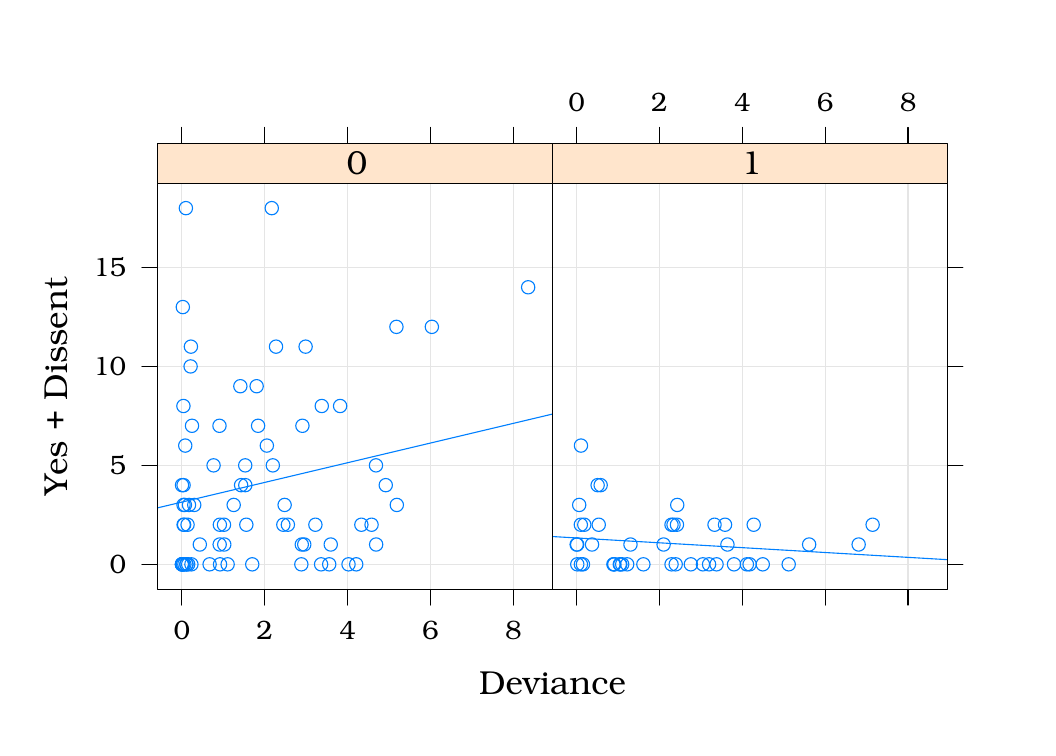
\begin{tikzpicture}[x=1pt,y=1pt]
\definecolor[named]{drawColor}{rgb}{0.00,0.00,0.00}
\definecolor[named]{fillColor}{rgb}{1.00,1.00,1.00}
\fill[color=fillColor,] (0,0) rectangle (361.35,252.94);
\begin{scope}
\path[clip] (  0.00,  0.00) rectangle (361.35,252.94);
\definecolor[named]{fillColor}{rgb}{0.00,0.00,0.00}
\end{scope}
\begin{scope}
\path[clip] (  0.00,  0.00) rectangle (361.35,252.94);
\definecolor[named]{fillColor}{rgb}{0.00,0.00,0.00}

\draw[fill opacity=0.00,draw opacity=0.00,] (  0.00,  0.00) rectangle (361.35,252.94);
\definecolor[named]{drawColor}{rgb}{0.00,0.00,0.00}

\node[color=drawColor,anchor=base,inner sep=0pt, outer sep=0pt, scale=  1.20] at (189.61, 12.04) {Deviance%
};
\end{scope}
\begin{scope}
\path[clip] (  0.00,  0.00) rectangle (361.35,252.94);
\definecolor[named]{fillColor}{rgb}{0.00,0.00,0.00}
\definecolor[named]{drawColor}{rgb}{0.00,0.00,0.00}

\node[rotate= 90.00,color=drawColor,anchor=base,inner sep=0pt, outer sep=0pt, scale=  1.20] at ( 14.29,123.38) {Yes + Dissent%
};
\end{scope}
\begin{scope}
\path[clip] (  0.00,  0.00) rectangle (361.35,252.94);
\definecolor[named]{fillColor}{rgb}{0.00,0.00,0.00}
\end{scope}
\begin{scope}
\path[clip] (  0.00,  0.00) rectangle (361.35,252.94);
\definecolor[named]{fillColor}{rgb}{0.00,0.00,0.00}
\end{scope}
\begin{scope}
\path[clip] (  0.00,  0.00) rectangle (361.35,252.94);
\definecolor[named]{fillColor}{rgb}{0.00,0.00,0.00}
\end{scope}
\begin{scope}
\path[clip] ( 46.98, 50.02) rectangle (189.61,196.74);
\definecolor[named]{fillColor}{rgb}{0.00,0.00,0.00}
\end{scope}
\begin{scope}
\path[clip] (  0.00,  0.00) rectangle (361.35,252.94);
\definecolor[named]{fillColor}{rgb}{0.00,0.00,0.00}
\end{scope}
\begin{scope}
\path[clip] (  0.00,  0.00) rectangle (361.35,252.94);
\definecolor[named]{fillColor}{rgb}{0.00,0.00,0.00}
\definecolor[named]{drawColor}{rgb}{0.00,0.00,0.00}

\draw[color=drawColor,line cap=round,line join=round,fill opacity=0.00,] ( 55.71,211.19) -- ( 55.71,216.88);

\draw[color=drawColor,line cap=round,line join=round,fill opacity=0.00,] ( 85.66,211.19) -- ( 85.66,216.88);

\draw[color=drawColor,line cap=round,line join=round,fill opacity=0.00,] (115.60,211.19) -- (115.60,216.88);

\draw[color=drawColor,line cap=round,line join=round,fill opacity=0.00,] (145.54,211.19) -- (145.54,216.88);

\draw[color=drawColor,line cap=round,line join=round,fill opacity=0.00,] (175.48,211.19) -- (175.48,216.88);
\end{scope}
\begin{scope}
\path[clip] (  0.00,  0.00) rectangle (361.35,252.94);
\definecolor[named]{fillColor}{rgb}{0.00,0.00,0.00}
\end{scope}
\begin{scope}
\path[clip] (  0.00,  0.00) rectangle (361.35,252.94);
\definecolor[named]{fillColor}{rgb}{0.00,0.00,0.00}
\definecolor[named]{drawColor}{rgb}{0.00,0.00,0.00}

\draw[color=drawColor,line cap=round,line join=round,fill opacity=0.00,] ( 46.98, 59.02) -- ( 41.29, 59.02);

\draw[color=drawColor,line cap=round,line join=round,fill opacity=0.00,] ( 46.98, 94.78) -- ( 41.29, 94.78);

\draw[color=drawColor,line cap=round,line join=round,fill opacity=0.00,] ( 46.98,130.53) -- ( 41.29,130.53);

\draw[color=drawColor,line cap=round,line join=round,fill opacity=0.00,] ( 46.98,166.28) -- ( 41.29,166.28);

\node[color=drawColor,anchor=base east,inner sep=0pt, outer sep=0pt, scale=  0.96] at ( 35.60, 55.72) {0%
};

\node[color=drawColor,anchor=base east,inner sep=0pt, outer sep=0pt, scale=  0.96] at ( 35.60, 91.47) {5%
};

\node[color=drawColor,anchor=base east,inner sep=0pt, outer sep=0pt, scale=  0.96] at ( 35.60,127.22) {10%
};

\node[color=drawColor,anchor=base east,inner sep=0pt, outer sep=0pt, scale=  0.96] at ( 35.60,162.97) {15%
};
\end{scope}
\begin{scope}
\path[clip] (  0.00,  0.00) rectangle (361.35,252.94);
\definecolor[named]{fillColor}{rgb}{0.00,0.00,0.00}
\end{scope}
\begin{scope}
\path[clip] (  0.00,  0.00) rectangle (361.35,252.94);
\definecolor[named]{fillColor}{rgb}{0.00,0.00,0.00}
\definecolor[named]{drawColor}{rgb}{0.00,0.00,0.00}

\draw[color=drawColor,line cap=round,line join=round,fill opacity=0.00,] ( 55.71, 50.02) -- ( 55.71, 44.32);

\draw[color=drawColor,line cap=round,line join=round,fill opacity=0.00,] ( 85.66, 50.02) -- ( 85.66, 44.32);

\draw[color=drawColor,line cap=round,line join=round,fill opacity=0.00,] (115.60, 50.02) -- (115.60, 44.32);

\draw[color=drawColor,line cap=round,line join=round,fill opacity=0.00,] (145.54, 50.02) -- (145.54, 44.32);

\draw[color=drawColor,line cap=round,line join=round,fill opacity=0.00,] (175.48, 50.02) -- (175.48, 44.32);

\node[color=drawColor,anchor=base,inner sep=0pt, outer sep=0pt, scale=  0.96] at ( 55.71, 32.02) {0%
};

\node[color=drawColor,anchor=base,inner sep=0pt, outer sep=0pt, scale=  0.96] at ( 85.66, 32.02) {2%
};

\node[color=drawColor,anchor=base,inner sep=0pt, outer sep=0pt, scale=  0.96] at (115.60, 32.02) {4%
};

\node[color=drawColor,anchor=base,inner sep=0pt, outer sep=0pt, scale=  0.96] at (145.54, 32.02) {6%
};

\node[color=drawColor,anchor=base,inner sep=0pt, outer sep=0pt, scale=  0.96] at (175.48, 32.02) {8%
};
\end{scope}
\begin{scope}
\path[clip] (  0.00,  0.00) rectangle (361.35,252.94);
\definecolor[named]{fillColor}{rgb}{0.00,0.00,0.00}
\end{scope}
\begin{scope}
\path[clip] ( 46.98, 50.02) rectangle (189.61,196.74);
\definecolor[named]{fillColor}{rgb}{0.00,0.00,0.00}
\definecolor[named]{drawColor}{rgb}{0.90,0.90,0.90}

\draw[color=drawColor,line cap=round,line join=round,fill opacity=0.00,] ( 46.98, 59.02) -- (189.61, 59.02);

\draw[color=drawColor,line cap=round,line join=round,fill opacity=0.00,] ( 46.98, 94.78) -- (189.61, 94.78);

\draw[color=drawColor,line cap=round,line join=round,fill opacity=0.00,] ( 46.98,130.53) -- (189.61,130.53);

\draw[color=drawColor,line cap=round,line join=round,fill opacity=0.00,] ( 46.98,166.28) -- (189.61,166.28);

\draw[color=drawColor,line cap=round,line join=round,fill opacity=0.00,] ( 55.71, 50.02) -- ( 55.71,196.74);

\draw[color=drawColor,line cap=round,line join=round,fill opacity=0.00,] ( 85.66, 50.02) -- ( 85.66,196.74);

\draw[color=drawColor,line cap=round,line join=round,fill opacity=0.00,] (115.60, 50.02) -- (115.60,196.74);

\draw[color=drawColor,line cap=round,line join=round,fill opacity=0.00,] (145.54, 50.02) -- (145.54,196.74);

\draw[color=drawColor,line cap=round,line join=round,fill opacity=0.00,] (175.48, 50.02) -- (175.48,196.74);
\definecolor[named]{drawColor}{rgb}{0.00,0.50,1.00}

\draw[color=drawColor,line cap=round,line join=round,fill opacity=0.00,] ( 58.00, 59.02) circle (  2.41);

\draw[color=drawColor,line cap=round,line join=round,fill opacity=0.00,] ( 58.30, 80.48) circle (  2.41);

\draw[color=drawColor,line cap=round,line join=round,fill opacity=0.00,] ( 59.17, 59.02) circle (  2.41);

\draw[color=drawColor,line cap=round,line join=round,fill opacity=0.00,] (125.86, 94.78) circle (  2.41);

\draw[color=drawColor,line cap=round,line join=round,fill opacity=0.00,] ( 60.19, 80.48) circle (  2.41);

\draw[color=drawColor,line cap=round,line join=round,fill opacity=0.00,] ( 92.38, 73.33) circle (  2.41);

\draw[color=drawColor,line cap=round,line join=round,fill opacity=0.00,] ( 70.94, 73.33) circle (  2.41);

\draw[color=drawColor,line cap=round,line join=round,fill opacity=0.00,] ( 55.79, 59.02) circle (  2.41);

\draw[color=drawColor,line cap=round,line join=round,fill opacity=0.00,] ( 56.21, 59.02) circle (  2.41);

\draw[color=drawColor,line cap=round,line join=round,fill opacity=0.00,] ( 56.64, 59.02) circle (  2.41);

\draw[color=drawColor,line cap=round,line join=round,fill opacity=0.00,] ( 69.31,109.08) circle (  2.41);

\draw[color=drawColor,line cap=round,line join=round,fill opacity=0.00,] ( 59.38,109.08) circle (  2.41);

\draw[color=drawColor,line cap=round,line join=round,fill opacity=0.00,] ( 56.81, 80.48) circle (  2.41);

\draw[color=drawColor,line cap=round,line join=round,fill opacity=0.00,] ( 57.40, 59.02) circle (  2.41);

\draw[color=drawColor,line cap=round,line join=round,fill opacity=0.00,] ( 89.74,137.68) circle (  2.41);

\draw[color=drawColor,line cap=round,line join=round,fill opacity=0.00,] (106.27,116.23) circle (  2.41);

\draw[color=drawColor,line cap=round,line join=round,fill opacity=0.00,] (103.97, 73.33) circle (  2.41);

\draw[color=drawColor,line cap=round,line join=round,fill opacity=0.00,] (106.03, 59.02) circle (  2.41);

\draw[color=drawColor,line cap=round,line join=round,fill opacity=0.00,] ( 56.94,101.93) circle (  2.41);

\draw[color=drawColor,line cap=round,line join=round,fill opacity=0.00,] ( 62.20, 66.18) circle (  2.41);

\draw[color=drawColor,line cap=round,line join=round,fill opacity=0.00,] ( 55.86, 59.02) circle (  2.41);

\draw[color=drawColor,line cap=round,line join=round,fill opacity=0.00,] ( 56.54, 73.33) circle (  2.41);

\draw[color=drawColor,line cap=round,line join=round,fill opacity=0.00,] ( 69.51, 59.02) circle (  2.41);

\draw[color=drawColor,line cap=round,line join=round,fill opacity=0.00,] ( 57.77, 73.33) circle (  2.41);

\draw[color=drawColor,line cap=round,line join=round,fill opacity=0.00,] ( 57.32, 59.02) circle (  2.41);

\draw[color=drawColor,line cap=round,line join=round,fill opacity=0.00,] (115.94, 59.02) circle (  2.41);

\draw[color=drawColor,line cap=round,line join=round,fill opacity=0.00,] (120.58, 73.33) circle (  2.41);

\draw[color=drawColor,line cap=round,line join=round,fill opacity=0.00,] (129.39, 87.63) circle (  2.41);

\draw[color=drawColor,line cap=round,line join=round,fill opacity=0.00,] ( 72.25, 59.02) circle (  2.41);

\draw[color=drawColor,line cap=round,line join=round,fill opacity=0.00,] ( 69.44, 73.33) circle (  2.41);

\draw[color=drawColor,line cap=round,line join=round,fill opacity=0.00,] ( 77.12, 87.63) circle (  2.41);

\draw[color=drawColor,line cap=round,line join=round,fill opacity=0.00,] ( 86.42,101.93) circle (  2.41);

\draw[color=drawColor,line cap=round,line join=round,fill opacity=0.00,] ( 57.17,187.73) circle (  2.41);

\draw[color=drawColor,line cap=round,line join=round,fill opacity=0.00,] (100.43,137.68) circle (  2.41);

\draw[color=drawColor,line cap=round,line join=round,fill opacity=0.00,] (146.05,144.83) circle (  2.41);

\draw[color=drawColor,line cap=round,line join=round,fill opacity=0.00,] ( 69.38, 66.18) circle (  2.41);

\draw[color=drawColor,line cap=round,line join=round,fill opacity=0.00,] ( 71.04, 66.18) circle (  2.41);

\draw[color=drawColor,line cap=round,line join=round,fill opacity=0.00,] ( 56.33, 87.63) circle (  2.41);

\draw[color=drawColor,line cap=round,line join=round,fill opacity=0.00,] ( 74.44, 80.48) circle (  2.41);

\draw[color=drawColor,line cap=round,line join=round,fill opacity=0.00,] (125.92, 66.18) circle (  2.41);

\draw[color=drawColor,line cap=round,line join=round,fill opacity=0.00,] ( 83.26,109.08) circle (  2.41);

\draw[color=drawColor,line cap=round,line join=round,fill opacity=0.00,] ( 55.78, 59.02) circle (  2.41);

\draw[color=drawColor,line cap=round,line join=round,fill opacity=0.00,] ( 55.74, 59.02) circle (  2.41);

\draw[color=drawColor,line cap=round,line join=round,fill opacity=0.00,] (124.26, 73.33) circle (  2.41);

\draw[color=drawColor,line cap=round,line join=round,fill opacity=0.00,] ( 88.58, 94.78) circle (  2.41);

\draw[color=drawColor,line cap=round,line join=round,fill opacity=0.00,] ( 99.94, 66.18) circle (  2.41);

\draw[color=drawColor,line cap=round,line join=round,fill opacity=0.00,] (108.96, 59.02) circle (  2.41);

\draw[color=drawColor,line cap=round,line join=round,fill opacity=0.00,] (109.51, 66.18) circle (  2.41);

\draw[color=drawColor,line cap=round,line join=round,fill opacity=0.00,] (118.72, 59.02) circle (  2.41);

\draw[color=drawColor,line cap=round,line join=round,fill opacity=0.00,] (133.39, 80.48) circle (  2.41);

\draw[color=drawColor,line cap=round,line join=round,fill opacity=0.00,] ( 65.74, 59.02) circle (  2.41);

\draw[color=drawColor,line cap=round,line join=round,fill opacity=0.00,] ( 92.85, 80.48) circle (  2.41);

\draw[color=drawColor,line cap=round,line join=round,fill opacity=0.00,] ( 55.77, 87.63) circle (  2.41);

\draw[color=drawColor,line cap=round,line join=round,fill opacity=0.00,] ( 55.80, 59.02) circle (  2.41);

\draw[color=drawColor,line cap=round,line join=round,fill opacity=0.00,] ( 81.15, 59.02) circle (  2.41);

\draw[color=drawColor,line cap=round,line join=round,fill opacity=0.00,] ( 56.28,116.23) circle (  2.41);

\draw[color=drawColor,line cap=round,line join=round,fill opacity=0.00,] ( 56.35, 73.33) circle (  2.41);

\draw[color=drawColor,line cap=round,line join=round,fill opacity=0.00,] ( 56.32, 80.48) circle (  2.41);

\draw[color=drawColor,line cap=round,line join=round,fill opacity=0.00,] ( 56.06,151.98) circle (  2.41);

\draw[color=drawColor,line cap=round,line join=round,fill opacity=0.00,] ( 78.61, 94.78) circle (  2.41);

\draw[color=drawColor,line cap=round,line join=round,fill opacity=0.00,] ( 58.87,130.53) circle (  2.41);

\draw[color=drawColor,line cap=round,line join=round,fill opacity=0.00,] ( 67.17, 94.78) circle (  2.41);

\draw[color=drawColor,line cap=round,line join=round,fill opacity=0.00,] ( 99.05, 66.18) circle (  2.41);

\draw[color=drawColor,line cap=round,line join=round,fill opacity=0.00,] ( 82.73,123.38) circle (  2.41);

\draw[color=drawColor,line cap=round,line join=round,fill opacity=0.00,] (180.85,159.13) circle (  2.41);

\draw[color=drawColor,line cap=round,line join=round,fill opacity=0.00,] (112.90,116.23) circle (  2.41);

\draw[color=drawColor,line cap=round,line join=round,fill opacity=0.00,] ( 99.28,109.08) circle (  2.41);

\draw[color=drawColor,line cap=round,line join=round,fill opacity=0.00,] ( 98.89, 59.02) circle (  2.41);

\draw[color=drawColor,line cap=round,line join=round,fill opacity=0.00,] ( 94.02, 73.33) circle (  2.41);

\draw[color=drawColor,line cap=round,line join=round,fill opacity=0.00,] (133.25,144.83) circle (  2.41);

\draw[color=drawColor,line cap=round,line join=round,fill opacity=0.00,] ( 79.01, 73.33) circle (  2.41);

\draw[color=drawColor,line cap=round,line join=round,fill opacity=0.00,] ( 58.98,137.68) circle (  2.41);

\draw[color=drawColor,line cap=round,line join=round,fill opacity=0.00,] ( 88.20,187.73) circle (  2.41);

\draw[color=drawColor,line cap=round,line join=round,fill opacity=0.00,] ( 76.85,123.38) circle (  2.41);

\draw[color=drawColor,line cap=round,line join=round,fill opacity=0.00,] ( 78.64, 87.63) circle (  2.41);

\draw[color=drawColor,line cap=round,line join=round,fill opacity=0.00,] (189.61,113.31) --
	( 46.98, 79.43);
\end{scope}
\begin{scope}
\path[clip] (  0.00,  0.00) rectangle (361.35,252.94);
\definecolor[named]{fillColor}{rgb}{0.00,0.00,0.00}
\end{scope}
\begin{scope}
\path[clip] (  0.00,  0.00) rectangle (361.35,252.94);
\definecolor[named]{fillColor}{rgb}{0.00,0.00,0.00}
\definecolor[named]{drawColor}{rgb}{0.00,0.00,0.00}

\draw[color=drawColor,line cap=round,line join=round,fill opacity=0.00,] ( 46.98, 50.02) rectangle (189.61,196.74);
\end{scope}
\begin{scope}
\path[clip] (  0.00,  0.00) rectangle (361.35,252.94);
\definecolor[named]{fillColor}{rgb}{0.00,0.00,0.00}
\end{scope}
\begin{scope}
\path[clip] (  0.00,  0.00) rectangle (361.35,252.94);
\definecolor[named]{fillColor}{rgb}{0.00,0.00,0.00}
\end{scope}
\begin{scope}
\path[clip] ( 46.98,196.74) rectangle (189.61,211.19);
\definecolor[named]{fillColor}{rgb}{0.00,0.00,0.00}
\definecolor[named]{drawColor}{rgb}{1.00,0.90,0.80}
\definecolor[named]{fillColor}{rgb}{1.00,0.90,0.80}

\draw[color=drawColor,line cap=round,line join=round,fill=fillColor,] ( 46.98,196.74) rectangle (189.61,211.19);
\definecolor[named]{drawColor}{rgb}{0.00,0.00,0.00}

\node[color=drawColor,anchor=base west,inner sep=0pt, outer sep=0pt, scale=  1.20] at (115.29,199.83) {0%
};
\end{scope}
\begin{scope}
\path[clip] (  0.00,  0.00) rectangle (361.35,252.94);
\definecolor[named]{fillColor}{rgb}{0.00,0.00,0.00}
\end{scope}
\begin{scope}
\path[clip] (  0.00,  0.00) rectangle (361.35,252.94);
\definecolor[named]{fillColor}{rgb}{0.00,0.00,0.00}
\definecolor[named]{drawColor}{rgb}{0.00,0.00,0.00}

\draw[color=drawColor,line cap=round,line join=round,fill opacity=0.00,] ( 46.98,196.74) rectangle (189.61,211.19);
\end{scope}
\begin{scope}
\path[clip] (  0.00,  0.00) rectangle (361.35,252.94);
\definecolor[named]{fillColor}{rgb}{0.00,0.00,0.00}
\end{scope}
\begin{scope}
\path[clip] (  0.00,  0.00) rectangle (361.35,252.94);
\definecolor[named]{fillColor}{rgb}{0.00,0.00,0.00}
\end{scope}
\begin{scope}
\path[clip] (189.61, 50.02) rectangle (332.23,196.74);
\definecolor[named]{fillColor}{rgb}{0.00,0.00,0.00}
\end{scope}
\begin{scope}
\path[clip] (  0.00,  0.00) rectangle (361.35,252.94);
\definecolor[named]{fillColor}{rgb}{0.00,0.00,0.00}
\end{scope}
\begin{scope}
\path[clip] (  0.00,  0.00) rectangle (361.35,252.94);
\definecolor[named]{fillColor}{rgb}{0.00,0.00,0.00}
\definecolor[named]{drawColor}{rgb}{0.00,0.00,0.00}

\draw[color=drawColor,line cap=round,line join=round,fill opacity=0.00,] (198.34,211.19) -- (198.34,216.88);

\draw[color=drawColor,line cap=round,line join=round,fill opacity=0.00,] (228.28,211.19) -- (228.28,216.88);

\draw[color=drawColor,line cap=round,line join=round,fill opacity=0.00,] (258.23,211.19) -- (258.23,216.88);

\draw[color=drawColor,line cap=round,line join=round,fill opacity=0.00,] (288.17,211.19) -- (288.17,216.88);

\draw[color=drawColor,line cap=round,line join=round,fill opacity=0.00,] (318.11,211.19) -- (318.11,216.88);

\node[color=drawColor,anchor=base,inner sep=0pt, outer sep=0pt, scale=  0.96] at (198.34,222.58) {0%
};

\node[color=drawColor,anchor=base,inner sep=0pt, outer sep=0pt, scale=  0.96] at (228.28,222.58) {2%
};

\node[color=drawColor,anchor=base,inner sep=0pt, outer sep=0pt, scale=  0.96] at (258.23,222.58) {4%
};

\node[color=drawColor,anchor=base,inner sep=0pt, outer sep=0pt, scale=  0.96] at (288.17,222.58) {6%
};

\node[color=drawColor,anchor=base,inner sep=0pt, outer sep=0pt, scale=  0.96] at (318.11,222.58) {8%
};
\end{scope}
\begin{scope}
\path[clip] (  0.00,  0.00) rectangle (361.35,252.94);
\definecolor[named]{fillColor}{rgb}{0.00,0.00,0.00}
\end{scope}
\begin{scope}
\path[clip] (  0.00,  0.00) rectangle (361.35,252.94);
\definecolor[named]{fillColor}{rgb}{0.00,0.00,0.00}
\end{scope}
\begin{scope}
\path[clip] (  0.00,  0.00) rectangle (361.35,252.94);
\definecolor[named]{fillColor}{rgb}{0.00,0.00,0.00}
\end{scope}
\begin{scope}
\path[clip] (  0.00,  0.00) rectangle (361.35,252.94);
\definecolor[named]{fillColor}{rgb}{0.00,0.00,0.00}
\definecolor[named]{drawColor}{rgb}{0.00,0.00,0.00}

\draw[color=drawColor,line cap=round,line join=round,fill opacity=0.00,] (198.34, 50.02) -- (198.34, 44.32);

\draw[color=drawColor,line cap=round,line join=round,fill opacity=0.00,] (228.28, 50.02) -- (228.28, 44.32);

\draw[color=drawColor,line cap=round,line join=round,fill opacity=0.00,] (258.23, 50.02) -- (258.23, 44.32);

\draw[color=drawColor,line cap=round,line join=round,fill opacity=0.00,] (288.17, 50.02) -- (288.17, 44.32);

\draw[color=drawColor,line cap=round,line join=round,fill opacity=0.00,] (318.11, 50.02) -- (318.11, 44.32);

\draw[color=drawColor,line cap=round,line join=round,fill opacity=0.00,] (332.23, 59.02) -- (337.92, 59.02);

\draw[color=drawColor,line cap=round,line join=round,fill opacity=0.00,] (332.23, 94.78) -- (337.92, 94.78);

\draw[color=drawColor,line cap=round,line join=round,fill opacity=0.00,] (332.23,130.53) -- (337.92,130.53);

\draw[color=drawColor,line cap=round,line join=round,fill opacity=0.00,] (332.23,166.28) -- (337.92,166.28);
\end{scope}
\begin{scope}
\path[clip] (  0.00,  0.00) rectangle (361.35,252.94);
\definecolor[named]{fillColor}{rgb}{0.00,0.00,0.00}
\end{scope}
\begin{scope}
\path[clip] (189.61, 50.02) rectangle (332.23,196.74);
\definecolor[named]{fillColor}{rgb}{0.00,0.00,0.00}
\definecolor[named]{drawColor}{rgb}{0.90,0.90,0.90}

\draw[color=drawColor,line cap=round,line join=round,fill opacity=0.00,] (189.61, 59.02) -- (332.23, 59.02);

\draw[color=drawColor,line cap=round,line join=round,fill opacity=0.00,] (189.61, 94.78) -- (332.23, 94.78);

\draw[color=drawColor,line cap=round,line join=round,fill opacity=0.00,] (189.61,130.53) -- (332.23,130.53);

\draw[color=drawColor,line cap=round,line join=round,fill opacity=0.00,] (189.61,166.28) -- (332.23,166.28);

\draw[color=drawColor,line cap=round,line join=round,fill opacity=0.00,] (198.34, 50.02) -- (198.34,196.74);

\draw[color=drawColor,line cap=round,line join=round,fill opacity=0.00,] (228.28, 50.02) -- (228.28,196.74);

\draw[color=drawColor,line cap=round,line join=round,fill opacity=0.00,] (258.23, 50.02) -- (258.23,196.74);

\draw[color=drawColor,line cap=round,line join=round,fill opacity=0.00,] (288.17, 50.02) -- (288.17,196.74);

\draw[color=drawColor,line cap=round,line join=round,fill opacity=0.00,] (318.11, 50.02) -- (318.11,196.74);
\definecolor[named]{drawColor}{rgb}{0.00,0.50,1.00}

\draw[color=drawColor,line cap=round,line join=round,fill opacity=0.00,] (211.98, 59.02) circle (  2.41);

\draw[color=drawColor,line cap=round,line join=round,fill opacity=0.00,] (262.35, 73.33) circle (  2.41);

\draw[color=drawColor,line cap=round,line join=round,fill opacity=0.00,] (234.72, 80.48) circle (  2.41);

\draw[color=drawColor,line cap=round,line join=round,fill opacity=0.00,] (214.15, 59.02) circle (  2.41);

\draw[color=drawColor,line cap=round,line join=round,fill opacity=0.00,] (198.57, 66.18) circle (  2.41);

\draw[color=drawColor,line cap=round,line join=round,fill opacity=0.00,] (198.38, 66.18) circle (  2.41);

\draw[color=drawColor,line cap=round,line join=round,fill opacity=0.00,] (198.60, 59.02) circle (  2.41);

\draw[color=drawColor,line cap=round,line join=round,fill opacity=0.00,] (246.22, 59.02) circle (  2.41);

\draw[color=drawColor,line cap=round,line join=round,fill opacity=0.00,] (203.93, 66.18) circle (  2.41);

\draw[color=drawColor,line cap=round,line join=round,fill opacity=0.00,] (199.93,101.93) circle (  2.41);

\draw[color=drawColor,line cap=round,line join=round,fill opacity=0.00,] (214.83, 59.02) circle (  2.41);

\draw[color=drawColor,line cap=round,line join=round,fill opacity=0.00,] (274.99, 59.02) circle (  2.41);

\draw[color=drawColor,line cap=round,line join=round,fill opacity=0.00,] (217.82, 66.18) circle (  2.41);

\draw[color=drawColor,line cap=round,line join=round,fill opacity=0.00,] (300.27, 66.18) circle (  2.41);

\draw[color=drawColor,line cap=round,line join=round,fill opacity=0.00,] (259.89, 59.02) circle (  2.41);

\draw[color=drawColor,line cap=round,line join=round,fill opacity=0.00,] (305.32, 73.33) circle (  2.41);

\draw[color=drawColor,line cap=round,line join=round,fill opacity=0.00,] (252.86, 66.18) circle (  2.41);

\draw[color=drawColor,line cap=round,line join=round,fill opacity=0.00,] (255.23, 59.02) circle (  2.41);

\draw[color=drawColor,line cap=round,line join=round,fill opacity=0.00,] (234.62, 73.33) circle (  2.41);

\draw[color=drawColor,line cap=round,line join=round,fill opacity=0.00,] (211.67, 59.02) circle (  2.41);

\draw[color=drawColor,line cap=round,line join=round,fill opacity=0.00,] (233.37, 73.33) circle (  2.41);

\draw[color=drawColor,line cap=round,line join=round,fill opacity=0.00,] (216.63, 59.02) circle (  2.41);

\draw[color=drawColor,line cap=round,line join=round,fill opacity=0.00,] (211.81, 59.02) circle (  2.41);

\draw[color=drawColor,line cap=round,line join=round,fill opacity=0.00,] (232.66, 59.02) circle (  2.41);

\draw[color=drawColor,line cap=round,line join=round,fill opacity=0.00,] (234.16, 59.02) circle (  2.41);

\draw[color=drawColor,line cap=round,line join=round,fill opacity=0.00,] (232.65, 73.33) circle (  2.41);

\draw[color=drawColor,line cap=round,line join=round,fill opacity=0.00,] (239.63, 59.02) circle (  2.41);

\draw[color=drawColor,line cap=round,line join=round,fill opacity=0.00,] (199.88, 73.33) circle (  2.41);

\draw[color=drawColor,line cap=round,line join=round,fill opacity=0.00,] (265.62, 59.02) circle (  2.41);

\draw[color=drawColor,line cap=round,line join=round,fill opacity=0.00,] (205.95, 87.63) circle (  2.41);

\draw[color=drawColor,line cap=round,line join=round,fill opacity=0.00,] (207.05, 87.63) circle (  2.41);

\draw[color=drawColor,line cap=round,line join=round,fill opacity=0.00,] (251.99, 73.33) circle (  2.41);

\draw[color=drawColor,line cap=round,line join=round,fill opacity=0.00,] (248.19, 73.33) circle (  2.41);

\draw[color=drawColor,line cap=round,line join=round,fill opacity=0.00,] (282.38, 66.18) circle (  2.41);

\draw[color=drawColor,line cap=round,line join=round,fill opacity=0.00,] (260.87, 59.02) circle (  2.41);

\draw[color=drawColor,line cap=round,line join=round,fill opacity=0.00,] (199.29, 80.48) circle (  2.41);

\draw[color=drawColor,line cap=round,line join=round,fill opacity=0.00,] (213.95, 59.02) circle (  2.41);

\draw[color=drawColor,line cap=round,line join=round,fill opacity=0.00,] (199.91, 59.02) circle (  2.41);

\draw[color=drawColor,line cap=round,line join=round,fill opacity=0.00,] (200.65, 59.02) circle (  2.41);

\draw[color=drawColor,line cap=round,line join=round,fill opacity=0.00,] (229.79, 66.18) circle (  2.41);

\draw[color=drawColor,line cap=round,line join=round,fill opacity=0.00,] (222.48, 59.02) circle (  2.41);

\draw[color=drawColor,line cap=round,line join=round,fill opacity=0.00,] (201.13, 73.33) circle (  2.41);

\draw[color=drawColor,line cap=round,line join=round,fill opacity=0.00,] (206.35, 73.33) circle (  2.41);

\draw[color=drawColor,line cap=round,line join=round,fill opacity=0.00,] (248.92, 59.02) circle (  2.41);

\draw[color=drawColor,line cap=round,line join=round,fill opacity=0.00,] (244.00, 59.02) circle (  2.41);

\draw[color=drawColor,line cap=round,line join=round,fill opacity=0.00,] (332.23, 60.71) --
	(189.61, 69.06);
\end{scope}
\begin{scope}
\path[clip] (  0.00,  0.00) rectangle (361.35,252.94);
\definecolor[named]{fillColor}{rgb}{0.00,0.00,0.00}
\end{scope}
\begin{scope}
\path[clip] (  0.00,  0.00) rectangle (361.35,252.94);
\definecolor[named]{fillColor}{rgb}{0.00,0.00,0.00}
\definecolor[named]{drawColor}{rgb}{0.00,0.00,0.00}

\draw[color=drawColor,line cap=round,line join=round,fill opacity=0.00,] (189.61, 50.02) rectangle (332.23,196.74);
\end{scope}
\begin{scope}
\path[clip] (  0.00,  0.00) rectangle (361.35,252.94);
\definecolor[named]{fillColor}{rgb}{0.00,0.00,0.00}
\end{scope}
\begin{scope}
\path[clip] (  0.00,  0.00) rectangle (361.35,252.94);
\definecolor[named]{fillColor}{rgb}{0.00,0.00,0.00}
\end{scope}
\begin{scope}
\path[clip] (189.61,196.74) rectangle (332.23,211.19);
\definecolor[named]{fillColor}{rgb}{0.00,0.00,0.00}
\definecolor[named]{drawColor}{rgb}{1.00,0.90,0.80}
\definecolor[named]{fillColor}{rgb}{1.00,0.90,0.80}

\draw[color=drawColor,line cap=round,line join=round,fill=fillColor,] (189.61,196.74) rectangle (332.23,211.19);
\definecolor[named]{drawColor}{rgb}{0.00,0.00,0.00}

\node[color=drawColor,anchor=base west,inner sep=0pt, outer sep=0pt, scale=  1.20] at (257.92,199.83) {1%
};
\end{scope}
\begin{scope}
\path[clip] (  0.00,  0.00) rectangle (361.35,252.94);
\definecolor[named]{fillColor}{rgb}{0.00,0.00,0.00}
\end{scope}
\begin{scope}
\path[clip] (  0.00,  0.00) rectangle (361.35,252.94);
\definecolor[named]{fillColor}{rgb}{0.00,0.00,0.00}
\definecolor[named]{drawColor}{rgb}{0.00,0.00,0.00}

\draw[color=drawColor,line cap=round,line join=round,fill opacity=0.00,] (189.61,196.74) rectangle (332.23,211.19);
\end{scope}
\begin{scope}
\path[clip] (  0.00,  0.00) rectangle (361.35,252.94);
\definecolor[named]{fillColor}{rgb}{0.00,0.00,0.00}
\end{scope}
\begin{scope}
\path[clip] (  0.00,  0.00) rectangle (361.35,252.94);
\definecolor[named]{fillColor}{rgb}{0.00,0.00,0.00}
\end{scope}
\begin{scope}
\path[clip] (  0.00,  0.00) rectangle (361.35,252.94);
\definecolor[named]{fillColor}{rgb}{0.00,0.00,0.00}
\end{scope}
\begin{scope}
\path[clip] (  0.00,  0.00) rectangle (361.35,252.94);
\definecolor[named]{fillColor}{rgb}{0.00,0.00,0.00}
\end{scope}
\end{tikzpicture}
}}\quad
\caption{The plot show the degree of deviance from the mean left-right position in the Council on the x-axis, and the number of abstentions on the y-axis. The values have been conditioned on whether a government was from an old or new member state.}
\label{fig:scatter}
\end{figure}

Consistently across all categories we see a positive relationship between deviance and the number of dissenting votes for old member states, and the opposite, although very weak, relationship for new member states. The plots show a somewhat surprising result as most of the literature on the Council show that there was no large effect of the eastern enlargement, but there does seem to be quite a large difference in voting behavior between governments from new and old member states. Hypothesis two is partly supported by Figure \ref{fig:scatter}, but only for old member states. New member states do not engage in dissenting behavior to the same extent as old member states, the modus operandi seem to be supportive of the outcome of Council negotiations, regardless of how much the deviate from the Council mean left-right position. Panel (b) in Figure \ref{fig:scatter} is not entirely expected, as the theory of diffuse reciprocity do not link no votes to being an outlier within in the Council, they are supposed to signal back home, despite that a government might be in favor of a dossier. One should be careful in interpreting the figures, though, as we cannot know how many cases there were an overlap of an outlying government that was also under domestic pressure to resist the result of the Council negotiations. We also see that yes votes with a dissenting statement increase as a government becomes more of an outlier in the Council, this is also what we would expect as in these instances the norm of diffuse reciprocity should be effective.  

The examine hypothesis three initially presents some obstacles. To avoid the effect of time, i.e. the longer a government has been in the Council the more likely it is to have cast a dissenting vote, the number of votes in a given choice category relative to the time spend in the Council were plotted, conditioned on the time spend in the council. The y-axis show the density within each category, while the x-axis show the relative voting frequency.

 
\begin{figure}[htp]
\centering
\scalebox{.6}{\subfloat[][No Votes]{% Created by tikzDevice version 0.6.1 on 2011-08-03 09:51:22
% !TEX encoding = UTF-8 Unicode
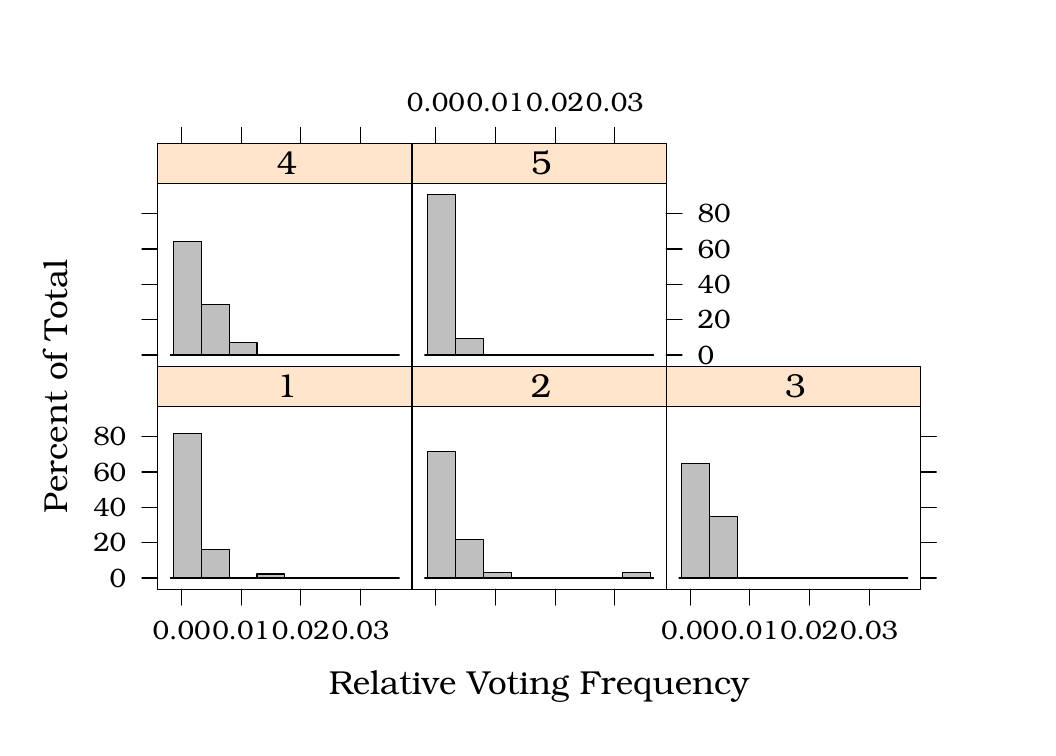
\begin{tikzpicture}[x=1pt,y=1pt]
\definecolor[named]{drawColor}{rgb}{0.00,0.00,0.00}
\definecolor[named]{fillColor}{rgb}{1.00,1.00,1.00}
\fill[color=fillColor,] (0,0) rectangle (361.35,252.94);
\begin{scope}
\path[clip] (  0.00,  0.00) rectangle (361.35,252.94);
\definecolor[named]{fillColor}{rgb}{0.00,0.00,0.00}
\end{scope}
\begin{scope}
\path[clip] (  0.00,  0.00) rectangle (361.35,252.94);
\definecolor[named]{fillColor}{rgb}{0.00,0.00,0.00}

\draw[fill opacity=0.00,draw opacity=0.00,] (  0.00,  0.00) rectangle (361.35,252.94);
\definecolor[named]{drawColor}{rgb}{0.00,0.00,0.00}

\node[color=drawColor,anchor=base,inner sep=0pt, outer sep=0pt, scale=  1.20] at (184.81, 12.04) {Relative Voting Frequency%
};
\end{scope}
\begin{scope}
\path[clip] (  0.00,  0.00) rectangle (361.35,252.94);
\definecolor[named]{fillColor}{rgb}{0.00,0.00,0.00}
\definecolor[named]{drawColor}{rgb}{0.00,0.00,0.00}

\node[rotate= 90.00,color=drawColor,anchor=base,inner sep=0pt, outer sep=0pt, scale=  1.20] at ( 14.29,123.38) {Percent of Total%
};
\end{scope}
\begin{scope}
\path[clip] (  0.00,  0.00) rectangle (361.35,252.94);
\definecolor[named]{fillColor}{rgb}{0.00,0.00,0.00}
\end{scope}
\begin{scope}
\path[clip] (  0.00,  0.00) rectangle (361.35,252.94);
\definecolor[named]{fillColor}{rgb}{0.00,0.00,0.00}
\end{scope}
\begin{scope}
\path[clip] (  0.00,  0.00) rectangle (361.35,252.94);
\definecolor[named]{fillColor}{rgb}{0.00,0.00,0.00}
\end{scope}
\begin{scope}
\path[clip] ( 46.98, 50.02) rectangle (138.86,116.15);
\definecolor[named]{fillColor}{rgb}{0.00,0.00,0.00}
\end{scope}
\begin{scope}
\path[clip] (  0.00,  0.00) rectangle (361.35,252.94);
\definecolor[named]{fillColor}{rgb}{0.00,0.00,0.00}
\end{scope}
\begin{scope}
\path[clip] (  0.00,  0.00) rectangle (361.35,252.94);
\definecolor[named]{fillColor}{rgb}{0.00,0.00,0.00}
\end{scope}
\begin{scope}
\path[clip] (  0.00,  0.00) rectangle (361.35,252.94);
\definecolor[named]{fillColor}{rgb}{0.00,0.00,0.00}
\end{scope}
\begin{scope}
\path[clip] (  0.00,  0.00) rectangle (361.35,252.94);
\definecolor[named]{fillColor}{rgb}{0.00,0.00,0.00}
\definecolor[named]{drawColor}{rgb}{0.00,0.00,0.00}

\draw[color=drawColor,line cap=round,line join=round,fill opacity=0.00,] ( 46.98, 54.08) -- ( 41.29, 54.08);

\draw[color=drawColor,line cap=round,line join=round,fill opacity=0.00,] ( 46.98, 66.84) -- ( 41.29, 66.84);

\draw[color=drawColor,line cap=round,line join=round,fill opacity=0.00,] ( 46.98, 79.60) -- ( 41.29, 79.60);

\draw[color=drawColor,line cap=round,line join=round,fill opacity=0.00,] ( 46.98, 92.37) -- ( 41.29, 92.37);

\draw[color=drawColor,line cap=round,line join=round,fill opacity=0.00,] ( 46.98,105.13) -- ( 41.29,105.13);

\node[color=drawColor,anchor=base east,inner sep=0pt, outer sep=0pt, scale=  0.96] at ( 35.60, 50.77) {0%
};

\node[color=drawColor,anchor=base east,inner sep=0pt, outer sep=0pt, scale=  0.96] at ( 35.60, 63.53) {20%
};

\node[color=drawColor,anchor=base east,inner sep=0pt, outer sep=0pt, scale=  0.96] at ( 35.60, 76.30) {40%
};

\node[color=drawColor,anchor=base east,inner sep=0pt, outer sep=0pt, scale=  0.96] at ( 35.60, 89.06) {60%
};

\node[color=drawColor,anchor=base east,inner sep=0pt, outer sep=0pt, scale=  0.96] at ( 35.60,101.82) {80%
};
\end{scope}
\begin{scope}
\path[clip] (  0.00,  0.00) rectangle (361.35,252.94);
\definecolor[named]{fillColor}{rgb}{0.00,0.00,0.00}
\end{scope}
\begin{scope}
\path[clip] (  0.00,  0.00) rectangle (361.35,252.94);
\definecolor[named]{fillColor}{rgb}{0.00,0.00,0.00}
\definecolor[named]{drawColor}{rgb}{0.00,0.00,0.00}

\draw[color=drawColor,line cap=round,line join=round,fill opacity=0.00,] ( 55.61, 50.02) -- ( 55.61, 44.32);

\draw[color=drawColor,line cap=round,line join=round,fill opacity=0.00,] ( 77.16, 50.02) -- ( 77.16, 44.32);

\draw[color=drawColor,line cap=round,line join=round,fill opacity=0.00,] ( 98.71, 50.02) -- ( 98.71, 44.32);

\draw[color=drawColor,line cap=round,line join=round,fill opacity=0.00,] (120.26, 50.02) -- (120.26, 44.32);

\node[color=drawColor,anchor=base,inner sep=0pt, outer sep=0pt, scale=  0.96] at ( 55.61, 32.02) {0.00%
};

\node[color=drawColor,anchor=base,inner sep=0pt, outer sep=0pt, scale=  0.96] at ( 77.16, 32.02) {0.01%
};

\node[color=drawColor,anchor=base,inner sep=0pt, outer sep=0pt, scale=  0.96] at ( 98.71, 32.02) {0.02%
};

\node[color=drawColor,anchor=base,inner sep=0pt, outer sep=0pt, scale=  0.96] at (120.26, 32.02) {0.03%
};
\end{scope}
\begin{scope}
\path[clip] (  0.00,  0.00) rectangle (361.35,252.94);
\definecolor[named]{fillColor}{rgb}{0.00,0.00,0.00}
\end{scope}
\begin{scope}
\path[clip] ( 46.98, 50.02) rectangle (138.86,116.15);
\definecolor[named]{fillColor}{rgb}{0.00,0.00,0.00}
\definecolor[named]{drawColor}{rgb}{0.00,0.00,0.00}

\draw[color=drawColor,line cap=round,line join=round,fill opacity=0.00,] ( 51.57, 54.08) --
	(134.27, 54.08);
\definecolor[named]{fillColor}{rgb}{0.75,0.75,0.75}

\draw[color=drawColor,line cap=round,line join=round,fill=fillColor,] ( 52.62, 54.08) rectangle ( 62.70,106.29);

\draw[color=drawColor,line cap=round,line join=round,fill=fillColor,] ( 62.70, 54.08) rectangle ( 72.77, 64.23);

\draw[color=drawColor,line cap=round,line join=round,fill=fillColor,] ( 72.77, 54.08) rectangle ( 82.85, 54.08);

\draw[color=drawColor,line cap=round,line join=round,fill=fillColor,] ( 82.85, 54.08) rectangle ( 92.92, 55.53);

\draw[color=drawColor,line cap=round,line join=round,fill=fillColor,] ( 92.92, 54.08) rectangle (103.00, 54.08);

\draw[color=drawColor,line cap=round,line join=round,fill=fillColor,] (103.00, 54.08) rectangle (113.07, 54.08);

\draw[color=drawColor,line cap=round,line join=round,fill=fillColor,] (113.07, 54.08) rectangle (123.15, 54.08);

\draw[color=drawColor,line cap=round,line join=round,fill=fillColor,] (123.15, 54.08) rectangle (133.22, 54.08);
\end{scope}
\begin{scope}
\path[clip] (  0.00,  0.00) rectangle (361.35,252.94);
\definecolor[named]{fillColor}{rgb}{0.00,0.00,0.00}
\end{scope}
\begin{scope}
\path[clip] (  0.00,  0.00) rectangle (361.35,252.94);
\definecolor[named]{fillColor}{rgb}{0.00,0.00,0.00}
\definecolor[named]{drawColor}{rgb}{0.00,0.00,0.00}

\draw[color=drawColor,line cap=round,line join=round,fill opacity=0.00,] ( 46.98, 50.02) rectangle (138.86,116.15);
\end{scope}
\begin{scope}
\path[clip] (  0.00,  0.00) rectangle (361.35,252.94);
\definecolor[named]{fillColor}{rgb}{0.00,0.00,0.00}
\end{scope}
\begin{scope}
\path[clip] (  0.00,  0.00) rectangle (361.35,252.94);
\definecolor[named]{fillColor}{rgb}{0.00,0.00,0.00}
\end{scope}
\begin{scope}
\path[clip] ( 46.98,116.15) rectangle (138.86,130.60);
\definecolor[named]{fillColor}{rgb}{0.00,0.00,0.00}
\definecolor[named]{drawColor}{rgb}{1.00,0.90,0.80}
\definecolor[named]{fillColor}{rgb}{1.00,0.90,0.80}

\draw[color=drawColor,line cap=round,line join=round,fill=fillColor,] ( 46.98,116.15) rectangle (138.86,130.60);
\definecolor[named]{drawColor}{rgb}{0.00,0.00,0.00}

\node[color=drawColor,anchor=base west,inner sep=0pt, outer sep=0pt, scale=  1.20] at ( 89.92,119.25) {1%
};
\end{scope}
\begin{scope}
\path[clip] (  0.00,  0.00) rectangle (361.35,252.94);
\definecolor[named]{fillColor}{rgb}{0.00,0.00,0.00}
\end{scope}
\begin{scope}
\path[clip] (  0.00,  0.00) rectangle (361.35,252.94);
\definecolor[named]{fillColor}{rgb}{0.00,0.00,0.00}
\definecolor[named]{drawColor}{rgb}{0.00,0.00,0.00}

\draw[color=drawColor,line cap=round,line join=round,fill opacity=0.00,] ( 46.98,116.15) rectangle (138.86,130.60);
\end{scope}
\begin{scope}
\path[clip] (  0.00,  0.00) rectangle (361.35,252.94);
\definecolor[named]{fillColor}{rgb}{0.00,0.00,0.00}
\end{scope}
\begin{scope}
\path[clip] (  0.00,  0.00) rectangle (361.35,252.94);
\definecolor[named]{fillColor}{rgb}{0.00,0.00,0.00}
\end{scope}
\begin{scope}
\path[clip] (138.86, 50.02) rectangle (230.75,116.15);
\definecolor[named]{fillColor}{rgb}{0.00,0.00,0.00}
\end{scope}
\begin{scope}
\path[clip] (  0.00,  0.00) rectangle (361.35,252.94);
\definecolor[named]{fillColor}{rgb}{0.00,0.00,0.00}
\end{scope}
\begin{scope}
\path[clip] (  0.00,  0.00) rectangle (361.35,252.94);
\definecolor[named]{fillColor}{rgb}{0.00,0.00,0.00}
\end{scope}
\begin{scope}
\path[clip] (  0.00,  0.00) rectangle (361.35,252.94);
\definecolor[named]{fillColor}{rgb}{0.00,0.00,0.00}
\end{scope}
\begin{scope}
\path[clip] (  0.00,  0.00) rectangle (361.35,252.94);
\definecolor[named]{fillColor}{rgb}{0.00,0.00,0.00}
\end{scope}
\begin{scope}
\path[clip] (  0.00,  0.00) rectangle (361.35,252.94);
\definecolor[named]{fillColor}{rgb}{0.00,0.00,0.00}
\end{scope}
\begin{scope}
\path[clip] (  0.00,  0.00) rectangle (361.35,252.94);
\definecolor[named]{fillColor}{rgb}{0.00,0.00,0.00}
\definecolor[named]{drawColor}{rgb}{0.00,0.00,0.00}

\draw[color=drawColor,line cap=round,line join=round,fill opacity=0.00,] (147.49, 50.02) -- (147.49, 44.32);

\draw[color=drawColor,line cap=round,line join=round,fill opacity=0.00,] (169.04, 50.02) -- (169.04, 44.32);

\draw[color=drawColor,line cap=round,line join=round,fill opacity=0.00,] (190.59, 50.02) -- (190.59, 44.32);

\draw[color=drawColor,line cap=round,line join=round,fill opacity=0.00,] (212.14, 50.02) -- (212.14, 44.32);
\end{scope}
\begin{scope}
\path[clip] (  0.00,  0.00) rectangle (361.35,252.94);
\definecolor[named]{fillColor}{rgb}{0.00,0.00,0.00}
\end{scope}
\begin{scope}
\path[clip] (138.86, 50.02) rectangle (230.75,116.15);
\definecolor[named]{fillColor}{rgb}{0.00,0.00,0.00}
\definecolor[named]{drawColor}{rgb}{0.00,0.00,0.00}

\draw[color=drawColor,line cap=round,line join=round,fill opacity=0.00,] (143.46, 54.08) --
	(226.16, 54.08);
\definecolor[named]{fillColor}{rgb}{0.75,0.75,0.75}

\draw[color=drawColor,line cap=round,line join=round,fill=fillColor,] (144.51, 54.08) rectangle (154.58, 99.94);

\draw[color=drawColor,line cap=round,line join=round,fill=fillColor,] (154.58, 54.08) rectangle (164.66, 68.04);

\draw[color=drawColor,line cap=round,line join=round,fill=fillColor,] (164.66, 54.08) rectangle (174.73, 56.07);

\draw[color=drawColor,line cap=round,line join=round,fill=fillColor,] (174.73, 54.08) rectangle (184.81, 54.08);

\draw[color=drawColor,line cap=round,line join=round,fill=fillColor,] (184.81, 54.08) rectangle (194.88, 54.08);

\draw[color=drawColor,line cap=round,line join=round,fill=fillColor,] (194.88, 54.08) rectangle (204.96, 54.08);

\draw[color=drawColor,line cap=round,line join=round,fill=fillColor,] (204.96, 54.08) rectangle (215.03, 54.08);

\draw[color=drawColor,line cap=round,line join=round,fill=fillColor,] (215.03, 54.08) rectangle (225.11, 56.07);
\end{scope}
\begin{scope}
\path[clip] (  0.00,  0.00) rectangle (361.35,252.94);
\definecolor[named]{fillColor}{rgb}{0.00,0.00,0.00}
\end{scope}
\begin{scope}
\path[clip] (  0.00,  0.00) rectangle (361.35,252.94);
\definecolor[named]{fillColor}{rgb}{0.00,0.00,0.00}
\definecolor[named]{drawColor}{rgb}{0.00,0.00,0.00}

\draw[color=drawColor,line cap=round,line join=round,fill opacity=0.00,] (138.86, 50.02) rectangle (230.75,116.15);
\end{scope}
\begin{scope}
\path[clip] (  0.00,  0.00) rectangle (361.35,252.94);
\definecolor[named]{fillColor}{rgb}{0.00,0.00,0.00}
\end{scope}
\begin{scope}
\path[clip] (  0.00,  0.00) rectangle (361.35,252.94);
\definecolor[named]{fillColor}{rgb}{0.00,0.00,0.00}
\end{scope}
\begin{scope}
\path[clip] (138.86,116.15) rectangle (230.75,130.60);
\definecolor[named]{fillColor}{rgb}{0.00,0.00,0.00}
\definecolor[named]{drawColor}{rgb}{1.00,0.90,0.80}
\definecolor[named]{fillColor}{rgb}{1.00,0.90,0.80}

\draw[color=drawColor,line cap=round,line join=round,fill=fillColor,] (138.86,116.15) rectangle (230.75,130.60);
\definecolor[named]{drawColor}{rgb}{0.00,0.00,0.00}

\node[color=drawColor,anchor=base west,inner sep=0pt, outer sep=0pt, scale=  1.20] at (181.81,119.25) {2%
};
\end{scope}
\begin{scope}
\path[clip] (  0.00,  0.00) rectangle (361.35,252.94);
\definecolor[named]{fillColor}{rgb}{0.00,0.00,0.00}
\end{scope}
\begin{scope}
\path[clip] (  0.00,  0.00) rectangle (361.35,252.94);
\definecolor[named]{fillColor}{rgb}{0.00,0.00,0.00}
\definecolor[named]{drawColor}{rgb}{0.00,0.00,0.00}

\draw[color=drawColor,line cap=round,line join=round,fill opacity=0.00,] (138.86,116.15) rectangle (230.75,130.60);
\end{scope}
\begin{scope}
\path[clip] (  0.00,  0.00) rectangle (361.35,252.94);
\definecolor[named]{fillColor}{rgb}{0.00,0.00,0.00}
\end{scope}
\begin{scope}
\path[clip] (  0.00,  0.00) rectangle (361.35,252.94);
\definecolor[named]{fillColor}{rgb}{0.00,0.00,0.00}
\end{scope}
\begin{scope}
\path[clip] (230.75, 50.02) rectangle (322.64,116.15);
\definecolor[named]{fillColor}{rgb}{0.00,0.00,0.00}
\end{scope}
\begin{scope}
\path[clip] (  0.00,  0.00) rectangle (361.35,252.94);
\definecolor[named]{fillColor}{rgb}{0.00,0.00,0.00}
\end{scope}
\begin{scope}
\path[clip] (  0.00,  0.00) rectangle (361.35,252.94);
\definecolor[named]{fillColor}{rgb}{0.00,0.00,0.00}
\end{scope}
\begin{scope}
\path[clip] (  0.00,  0.00) rectangle (361.35,252.94);
\definecolor[named]{fillColor}{rgb}{0.00,0.00,0.00}
\end{scope}
\begin{scope}
\path[clip] (  0.00,  0.00) rectangle (361.35,252.94);
\definecolor[named]{fillColor}{rgb}{0.00,0.00,0.00}
\end{scope}
\begin{scope}
\path[clip] (  0.00,  0.00) rectangle (361.35,252.94);
\definecolor[named]{fillColor}{rgb}{0.00,0.00,0.00}
\end{scope}
\begin{scope}
\path[clip] (  0.00,  0.00) rectangle (361.35,252.94);
\definecolor[named]{fillColor}{rgb}{0.00,0.00,0.00}
\definecolor[named]{drawColor}{rgb}{0.00,0.00,0.00}

\draw[color=drawColor,line cap=round,line join=round,fill opacity=0.00,] (239.38, 50.02) -- (239.38, 44.32);

\draw[color=drawColor,line cap=round,line join=round,fill opacity=0.00,] (260.93, 50.02) -- (260.93, 44.32);

\draw[color=drawColor,line cap=round,line join=round,fill opacity=0.00,] (282.48, 50.02) -- (282.48, 44.32);

\draw[color=drawColor,line cap=round,line join=round,fill opacity=0.00,] (304.03, 50.02) -- (304.03, 44.32);

\node[color=drawColor,anchor=base,inner sep=0pt, outer sep=0pt, scale=  0.96] at (239.38, 32.02) {0.00%
};

\node[color=drawColor,anchor=base,inner sep=0pt, outer sep=0pt, scale=  0.96] at (260.93, 32.02) {0.01%
};

\node[color=drawColor,anchor=base,inner sep=0pt, outer sep=0pt, scale=  0.96] at (282.48, 32.02) {0.02%
};

\node[color=drawColor,anchor=base,inner sep=0pt, outer sep=0pt, scale=  0.96] at (304.03, 32.02) {0.03%
};

\draw[color=drawColor,line cap=round,line join=round,fill opacity=0.00,] (322.64, 54.08) -- (328.33, 54.08);

\draw[color=drawColor,line cap=round,line join=round,fill opacity=0.00,] (322.64, 66.84) -- (328.33, 66.84);

\draw[color=drawColor,line cap=round,line join=round,fill opacity=0.00,] (322.64, 79.60) -- (328.33, 79.60);

\draw[color=drawColor,line cap=round,line join=round,fill opacity=0.00,] (322.64, 92.37) -- (328.33, 92.37);

\draw[color=drawColor,line cap=round,line join=round,fill opacity=0.00,] (322.64,105.13) -- (328.33,105.13);
\end{scope}
\begin{scope}
\path[clip] (  0.00,  0.00) rectangle (361.35,252.94);
\definecolor[named]{fillColor}{rgb}{0.00,0.00,0.00}
\end{scope}
\begin{scope}
\path[clip] (230.75, 50.02) rectangle (322.64,116.15);
\definecolor[named]{fillColor}{rgb}{0.00,0.00,0.00}
\definecolor[named]{drawColor}{rgb}{0.00,0.00,0.00}

\draw[color=drawColor,line cap=round,line join=round,fill opacity=0.00,] (235.34, 54.08) --
	(318.04, 54.08);
\definecolor[named]{fillColor}{rgb}{0.75,0.75,0.75}

\draw[color=drawColor,line cap=round,line join=round,fill=fillColor,] (236.39, 54.08) rectangle (246.47, 95.56);

\draw[color=drawColor,line cap=round,line join=round,fill=fillColor,] (246.47, 54.08) rectangle (256.54, 76.41);

\draw[color=drawColor,line cap=round,line join=round,fill=fillColor,] (256.54, 54.08) rectangle (266.62, 54.08);

\draw[color=drawColor,line cap=round,line join=round,fill=fillColor,] (266.62, 54.08) rectangle (276.69, 54.08);

\draw[color=drawColor,line cap=round,line join=round,fill=fillColor,] (276.69, 54.08) rectangle (286.77, 54.08);

\draw[color=drawColor,line cap=round,line join=round,fill=fillColor,] (286.77, 54.08) rectangle (296.84, 54.08);

\draw[color=drawColor,line cap=round,line join=round,fill=fillColor,] (296.84, 54.08) rectangle (306.92, 54.08);

\draw[color=drawColor,line cap=round,line join=round,fill=fillColor,] (306.92, 54.08) rectangle (316.99, 54.08);
\end{scope}
\begin{scope}
\path[clip] (  0.00,  0.00) rectangle (361.35,252.94);
\definecolor[named]{fillColor}{rgb}{0.00,0.00,0.00}
\end{scope}
\begin{scope}
\path[clip] (  0.00,  0.00) rectangle (361.35,252.94);
\definecolor[named]{fillColor}{rgb}{0.00,0.00,0.00}
\definecolor[named]{drawColor}{rgb}{0.00,0.00,0.00}

\draw[color=drawColor,line cap=round,line join=round,fill opacity=0.00,] (230.75, 50.02) rectangle (322.64,116.15);
\end{scope}
\begin{scope}
\path[clip] (  0.00,  0.00) rectangle (361.35,252.94);
\definecolor[named]{fillColor}{rgb}{0.00,0.00,0.00}
\end{scope}
\begin{scope}
\path[clip] (  0.00,  0.00) rectangle (361.35,252.94);
\definecolor[named]{fillColor}{rgb}{0.00,0.00,0.00}
\end{scope}
\begin{scope}
\path[clip] (230.75,116.15) rectangle (322.64,130.60);
\definecolor[named]{fillColor}{rgb}{0.00,0.00,0.00}
\definecolor[named]{drawColor}{rgb}{1.00,0.90,0.80}
\definecolor[named]{fillColor}{rgb}{1.00,0.90,0.80}

\draw[color=drawColor,line cap=round,line join=round,fill=fillColor,] (230.75,116.15) rectangle (322.64,130.60);
\definecolor[named]{drawColor}{rgb}{0.00,0.00,0.00}

\node[color=drawColor,anchor=base west,inner sep=0pt, outer sep=0pt, scale=  1.20] at (273.69,119.25) {3%
};
\end{scope}
\begin{scope}
\path[clip] (  0.00,  0.00) rectangle (361.35,252.94);
\definecolor[named]{fillColor}{rgb}{0.00,0.00,0.00}
\end{scope}
\begin{scope}
\path[clip] (  0.00,  0.00) rectangle (361.35,252.94);
\definecolor[named]{fillColor}{rgb}{0.00,0.00,0.00}
\definecolor[named]{drawColor}{rgb}{0.00,0.00,0.00}

\draw[color=drawColor,line cap=round,line join=round,fill opacity=0.00,] (230.75,116.15) rectangle (322.64,130.60);
\end{scope}
\begin{scope}
\path[clip] (  0.00,  0.00) rectangle (361.35,252.94);
\definecolor[named]{fillColor}{rgb}{0.00,0.00,0.00}
\end{scope}
\begin{scope}
\path[clip] (  0.00,  0.00) rectangle (361.35,252.94);
\definecolor[named]{fillColor}{rgb}{0.00,0.00,0.00}
\end{scope}
\begin{scope}
\path[clip] ( 46.98,130.60) rectangle (138.86,196.74);
\definecolor[named]{fillColor}{rgb}{0.00,0.00,0.00}
\end{scope}
\begin{scope}
\path[clip] (  0.00,  0.00) rectangle (361.35,252.94);
\definecolor[named]{fillColor}{rgb}{0.00,0.00,0.00}
\end{scope}
\begin{scope}
\path[clip] (  0.00,  0.00) rectangle (361.35,252.94);
\definecolor[named]{fillColor}{rgb}{0.00,0.00,0.00}
\definecolor[named]{drawColor}{rgb}{0.00,0.00,0.00}

\draw[color=drawColor,line cap=round,line join=round,fill opacity=0.00,] ( 55.61,211.19) -- ( 55.61,216.88);

\draw[color=drawColor,line cap=round,line join=round,fill opacity=0.00,] ( 77.16,211.19) -- ( 77.16,216.88);

\draw[color=drawColor,line cap=round,line join=round,fill opacity=0.00,] ( 98.71,211.19) -- ( 98.71,216.88);

\draw[color=drawColor,line cap=round,line join=round,fill opacity=0.00,] (120.26,211.19) -- (120.26,216.88);
\end{scope}
\begin{scope}
\path[clip] (  0.00,  0.00) rectangle (361.35,252.94);
\definecolor[named]{fillColor}{rgb}{0.00,0.00,0.00}
\end{scope}
\begin{scope}
\path[clip] (  0.00,  0.00) rectangle (361.35,252.94);
\definecolor[named]{fillColor}{rgb}{0.00,0.00,0.00}
\definecolor[named]{drawColor}{rgb}{0.00,0.00,0.00}

\draw[color=drawColor,line cap=round,line join=round,fill opacity=0.00,] ( 46.98,134.67) -- ( 41.29,134.67);

\draw[color=drawColor,line cap=round,line join=round,fill opacity=0.00,] ( 46.98,147.43) -- ( 41.29,147.43);

\draw[color=drawColor,line cap=round,line join=round,fill opacity=0.00,] ( 46.98,160.19) -- ( 41.29,160.19);

\draw[color=drawColor,line cap=round,line join=round,fill opacity=0.00,] ( 46.98,172.95) -- ( 41.29,172.95);

\draw[color=drawColor,line cap=round,line join=round,fill opacity=0.00,] ( 46.98,185.72) -- ( 41.29,185.72);
\end{scope}
\begin{scope}
\path[clip] (  0.00,  0.00) rectangle (361.35,252.94);
\definecolor[named]{fillColor}{rgb}{0.00,0.00,0.00}
\end{scope}
\begin{scope}
\path[clip] (  0.00,  0.00) rectangle (361.35,252.94);
\definecolor[named]{fillColor}{rgb}{0.00,0.00,0.00}
\end{scope}
\begin{scope}
\path[clip] (  0.00,  0.00) rectangle (361.35,252.94);
\definecolor[named]{fillColor}{rgb}{0.00,0.00,0.00}
\end{scope}
\begin{scope}
\path[clip] ( 46.98,130.60) rectangle (138.86,196.74);
\definecolor[named]{fillColor}{rgb}{0.00,0.00,0.00}
\definecolor[named]{drawColor}{rgb}{0.00,0.00,0.00}

\draw[color=drawColor,line cap=round,line join=round,fill opacity=0.00,] ( 51.57,134.67) --
	(134.27,134.67);
\definecolor[named]{fillColor}{rgb}{0.75,0.75,0.75}

\draw[color=drawColor,line cap=round,line join=round,fill=fillColor,] ( 52.62,134.67) rectangle ( 62.70,175.69);

\draw[color=drawColor,line cap=round,line join=round,fill=fillColor,] ( 62.70,134.67) rectangle ( 72.77,152.90);

\draw[color=drawColor,line cap=round,line join=round,fill=fillColor,] ( 72.77,134.67) rectangle ( 82.85,139.22);

\draw[color=drawColor,line cap=round,line join=round,fill=fillColor,] ( 82.85,134.67) rectangle ( 92.92,134.67);

\draw[color=drawColor,line cap=round,line join=round,fill=fillColor,] ( 92.92,134.67) rectangle (103.00,134.67);

\draw[color=drawColor,line cap=round,line join=round,fill=fillColor,] (103.00,134.67) rectangle (113.07,134.67);

\draw[color=drawColor,line cap=round,line join=round,fill=fillColor,] (113.07,134.67) rectangle (123.15,134.67);

\draw[color=drawColor,line cap=round,line join=round,fill=fillColor,] (123.15,134.67) rectangle (133.22,134.67);
\end{scope}
\begin{scope}
\path[clip] (  0.00,  0.00) rectangle (361.35,252.94);
\definecolor[named]{fillColor}{rgb}{0.00,0.00,0.00}
\end{scope}
\begin{scope}
\path[clip] (  0.00,  0.00) rectangle (361.35,252.94);
\definecolor[named]{fillColor}{rgb}{0.00,0.00,0.00}
\definecolor[named]{drawColor}{rgb}{0.00,0.00,0.00}

\draw[color=drawColor,line cap=round,line join=round,fill opacity=0.00,] ( 46.98,130.60) rectangle (138.86,196.74);
\end{scope}
\begin{scope}
\path[clip] (  0.00,  0.00) rectangle (361.35,252.94);
\definecolor[named]{fillColor}{rgb}{0.00,0.00,0.00}
\end{scope}
\begin{scope}
\path[clip] (  0.00,  0.00) rectangle (361.35,252.94);
\definecolor[named]{fillColor}{rgb}{0.00,0.00,0.00}
\end{scope}
\begin{scope}
\path[clip] ( 46.98,196.74) rectangle (138.86,211.19);
\definecolor[named]{fillColor}{rgb}{0.00,0.00,0.00}
\definecolor[named]{drawColor}{rgb}{1.00,0.90,0.80}
\definecolor[named]{fillColor}{rgb}{1.00,0.90,0.80}

\draw[color=drawColor,line cap=round,line join=round,fill=fillColor,] ( 46.98,196.74) rectangle (138.86,211.19);
\definecolor[named]{drawColor}{rgb}{0.00,0.00,0.00}

\node[color=drawColor,anchor=base west,inner sep=0pt, outer sep=0pt, scale=  1.20] at ( 89.92,199.83) {4%
};
\end{scope}
\begin{scope}
\path[clip] (  0.00,  0.00) rectangle (361.35,252.94);
\definecolor[named]{fillColor}{rgb}{0.00,0.00,0.00}
\end{scope}
\begin{scope}
\path[clip] (  0.00,  0.00) rectangle (361.35,252.94);
\definecolor[named]{fillColor}{rgb}{0.00,0.00,0.00}
\definecolor[named]{drawColor}{rgb}{0.00,0.00,0.00}

\draw[color=drawColor,line cap=round,line join=round,fill opacity=0.00,] ( 46.98,196.74) rectangle (138.86,211.19);
\end{scope}
\begin{scope}
\path[clip] (  0.00,  0.00) rectangle (361.35,252.94);
\definecolor[named]{fillColor}{rgb}{0.00,0.00,0.00}
\end{scope}
\begin{scope}
\path[clip] (  0.00,  0.00) rectangle (361.35,252.94);
\definecolor[named]{fillColor}{rgb}{0.00,0.00,0.00}
\end{scope}
\begin{scope}
\path[clip] (138.86,130.60) rectangle (230.75,196.74);
\definecolor[named]{fillColor}{rgb}{0.00,0.00,0.00}
\end{scope}
\begin{scope}
\path[clip] (  0.00,  0.00) rectangle (361.35,252.94);
\definecolor[named]{fillColor}{rgb}{0.00,0.00,0.00}
\end{scope}
\begin{scope}
\path[clip] (  0.00,  0.00) rectangle (361.35,252.94);
\definecolor[named]{fillColor}{rgb}{0.00,0.00,0.00}
\definecolor[named]{drawColor}{rgb}{0.00,0.00,0.00}

\draw[color=drawColor,line cap=round,line join=round,fill opacity=0.00,] (147.49,211.19) -- (147.49,216.88);

\draw[color=drawColor,line cap=round,line join=round,fill opacity=0.00,] (169.04,211.19) -- (169.04,216.88);

\draw[color=drawColor,line cap=round,line join=round,fill opacity=0.00,] (190.59,211.19) -- (190.59,216.88);

\draw[color=drawColor,line cap=round,line join=round,fill opacity=0.00,] (212.14,211.19) -- (212.14,216.88);

\node[color=drawColor,anchor=base,inner sep=0pt, outer sep=0pt, scale=  0.96] at (147.49,222.58) {0.00%
};

\node[color=drawColor,anchor=base,inner sep=0pt, outer sep=0pt, scale=  0.96] at (169.04,222.58) {0.01%
};

\node[color=drawColor,anchor=base,inner sep=0pt, outer sep=0pt, scale=  0.96] at (190.59,222.58) {0.02%
};

\node[color=drawColor,anchor=base,inner sep=0pt, outer sep=0pt, scale=  0.96] at (212.14,222.58) {0.03%
};
\end{scope}
\begin{scope}
\path[clip] (  0.00,  0.00) rectangle (361.35,252.94);
\definecolor[named]{fillColor}{rgb}{0.00,0.00,0.00}
\end{scope}
\begin{scope}
\path[clip] (  0.00,  0.00) rectangle (361.35,252.94);
\definecolor[named]{fillColor}{rgb}{0.00,0.00,0.00}
\end{scope}
\begin{scope}
\path[clip] (  0.00,  0.00) rectangle (361.35,252.94);
\definecolor[named]{fillColor}{rgb}{0.00,0.00,0.00}
\end{scope}
\begin{scope}
\path[clip] (  0.00,  0.00) rectangle (361.35,252.94);
\definecolor[named]{fillColor}{rgb}{0.00,0.00,0.00}
\definecolor[named]{drawColor}{rgb}{0.00,0.00,0.00}

\draw[color=drawColor,line cap=round,line join=round,fill opacity=0.00,] (230.75,134.67) -- (236.44,134.67);

\draw[color=drawColor,line cap=round,line join=round,fill opacity=0.00,] (230.75,147.43) -- (236.44,147.43);

\draw[color=drawColor,line cap=round,line join=round,fill opacity=0.00,] (230.75,160.19) -- (236.44,160.19);

\draw[color=drawColor,line cap=round,line join=round,fill opacity=0.00,] (230.75,172.95) -- (236.44,172.95);

\draw[color=drawColor,line cap=round,line join=round,fill opacity=0.00,] (230.75,185.72) -- (236.44,185.72);

\node[color=drawColor,anchor=base west,inner sep=0pt, outer sep=0pt, scale=  0.96] at (242.13,131.36) {0%
};

\node[color=drawColor,anchor=base west,inner sep=0pt, outer sep=0pt, scale=  0.96] at (242.13,144.12) {20%
};

\node[color=drawColor,anchor=base west,inner sep=0pt, outer sep=0pt, scale=  0.96] at (242.13,156.89) {40%
};

\node[color=drawColor,anchor=base west,inner sep=0pt, outer sep=0pt, scale=  0.96] at (242.13,169.65) {60%
};

\node[color=drawColor,anchor=base west,inner sep=0pt, outer sep=0pt, scale=  0.96] at (242.13,182.41) {80%
};
\end{scope}
\begin{scope}
\path[clip] (  0.00,  0.00) rectangle (361.35,252.94);
\definecolor[named]{fillColor}{rgb}{0.00,0.00,0.00}
\end{scope}
\begin{scope}
\path[clip] (138.86,130.60) rectangle (230.75,196.74);
\definecolor[named]{fillColor}{rgb}{0.00,0.00,0.00}
\definecolor[named]{drawColor}{rgb}{0.00,0.00,0.00}

\draw[color=drawColor,line cap=round,line join=round,fill opacity=0.00,] (143.46,134.67) --
	(226.16,134.67);
\definecolor[named]{fillColor}{rgb}{0.75,0.75,0.75}

\draw[color=drawColor,line cap=round,line join=round,fill=fillColor,] (144.51,134.67) rectangle (154.58,192.68);

\draw[color=drawColor,line cap=round,line join=round,fill=fillColor,] (154.58,134.67) rectangle (164.66,140.47);

\draw[color=drawColor,line cap=round,line join=round,fill=fillColor,] (164.66,134.67) rectangle (174.73,134.67);

\draw[color=drawColor,line cap=round,line join=round,fill=fillColor,] (174.73,134.67) rectangle (184.81,134.67);

\draw[color=drawColor,line cap=round,line join=round,fill=fillColor,] (184.81,134.67) rectangle (194.88,134.67);

\draw[color=drawColor,line cap=round,line join=round,fill=fillColor,] (194.88,134.67) rectangle (204.96,134.67);

\draw[color=drawColor,line cap=round,line join=round,fill=fillColor,] (204.96,134.67) rectangle (215.03,134.67);

\draw[color=drawColor,line cap=round,line join=round,fill=fillColor,] (215.03,134.67) rectangle (225.11,134.67);
\end{scope}
\begin{scope}
\path[clip] (  0.00,  0.00) rectangle (361.35,252.94);
\definecolor[named]{fillColor}{rgb}{0.00,0.00,0.00}
\end{scope}
\begin{scope}
\path[clip] (  0.00,  0.00) rectangle (361.35,252.94);
\definecolor[named]{fillColor}{rgb}{0.00,0.00,0.00}
\definecolor[named]{drawColor}{rgb}{0.00,0.00,0.00}

\draw[color=drawColor,line cap=round,line join=round,fill opacity=0.00,] (138.86,130.60) rectangle (230.75,196.74);
\end{scope}
\begin{scope}
\path[clip] (  0.00,  0.00) rectangle (361.35,252.94);
\definecolor[named]{fillColor}{rgb}{0.00,0.00,0.00}
\end{scope}
\begin{scope}
\path[clip] (  0.00,  0.00) rectangle (361.35,252.94);
\definecolor[named]{fillColor}{rgb}{0.00,0.00,0.00}
\end{scope}
\begin{scope}
\path[clip] (138.86,196.74) rectangle (230.75,211.19);
\definecolor[named]{fillColor}{rgb}{0.00,0.00,0.00}
\definecolor[named]{drawColor}{rgb}{1.00,0.90,0.80}
\definecolor[named]{fillColor}{rgb}{1.00,0.90,0.80}

\draw[color=drawColor,line cap=round,line join=round,fill=fillColor,] (138.86,196.74) rectangle (230.75,211.19);
\definecolor[named]{drawColor}{rgb}{0.00,0.00,0.00}

\node[color=drawColor,anchor=base west,inner sep=0pt, outer sep=0pt, scale=  1.20] at (181.81,199.83) {5%
};
\end{scope}
\begin{scope}
\path[clip] (  0.00,  0.00) rectangle (361.35,252.94);
\definecolor[named]{fillColor}{rgb}{0.00,0.00,0.00}
\end{scope}
\begin{scope}
\path[clip] (  0.00,  0.00) rectangle (361.35,252.94);
\definecolor[named]{fillColor}{rgb}{0.00,0.00,0.00}
\definecolor[named]{drawColor}{rgb}{0.00,0.00,0.00}

\draw[color=drawColor,line cap=round,line join=round,fill opacity=0.00,] (138.86,196.74) rectangle (230.75,211.19);
\end{scope}
\begin{scope}
\path[clip] (  0.00,  0.00) rectangle (361.35,252.94);
\definecolor[named]{fillColor}{rgb}{0.00,0.00,0.00}
\end{scope}
\begin{scope}
\path[clip] (  0.00,  0.00) rectangle (361.35,252.94);
\definecolor[named]{fillColor}{rgb}{0.00,0.00,0.00}
\end{scope}
\begin{scope}
\path[clip] (  0.00,  0.00) rectangle (361.35,252.94);
\definecolor[named]{fillColor}{rgb}{0.00,0.00,0.00}
\end{scope}
\begin{scope}
\path[clip] (  0.00,  0.00) rectangle (361.35,252.94);
\definecolor[named]{fillColor}{rgb}{0.00,0.00,0.00}
\end{scope}
\end{tikzpicture}
}}\quad
\scalebox{.6}{\subfloat[][Abstentions]{% Created by tikzDevice version 0.6.1 on 2011-07-24 21:12:41
% !TEX encoding = UTF-8 Unicode
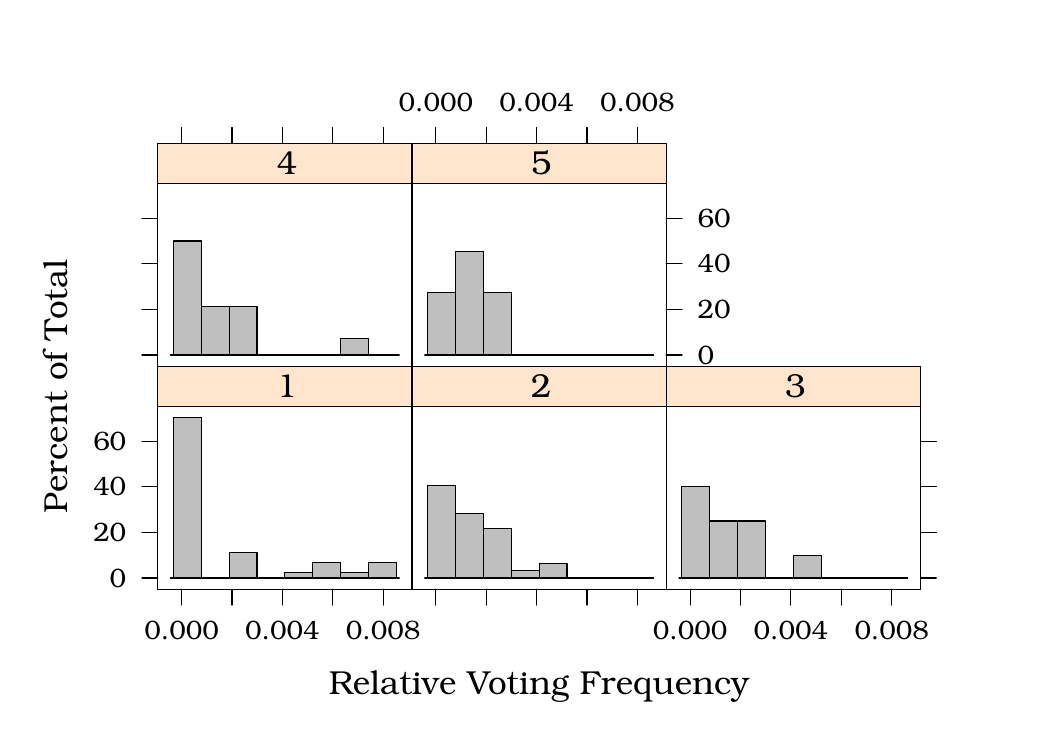
\begin{tikzpicture}[x=1pt,y=1pt]
\definecolor[named]{drawColor}{rgb}{0.00,0.00,0.00}
\definecolor[named]{fillColor}{rgb}{1.00,1.00,1.00}
\fill[color=fillColor,] (0,0) rectangle (361.35,252.94);
\begin{scope}
\path[clip] (  0.00,  0.00) rectangle (361.35,252.94);
\end{scope}
\begin{scope}
\path[clip] (  0.00,  0.00) rectangle (361.35,252.94);

\draw[fill opacity=0.00,draw opacity=0.00,] (  0.00,  0.00) rectangle (361.35,252.94);
\definecolor[named]{drawColor}{rgb}{0.00,0.00,0.00}

\node[color=drawColor,anchor=base,inner sep=0pt, outer sep=0pt, scale=  1.20] at (184.81, 12.04) {Relative Voting Frequency%
};
\end{scope}
\begin{scope}
\path[clip] (  0.00,  0.00) rectangle (361.35,252.94);
\definecolor[named]{drawColor}{rgb}{0.00,0.00,0.00}

\node[rotate= 90.00,color=drawColor,anchor=base,inner sep=0pt, outer sep=0pt, scale=  1.20] at ( 14.29,123.38) {Percent of Total%
};
\end{scope}
\begin{scope}
\path[clip] (  0.00,  0.00) rectangle (361.35,252.94);
\end{scope}
\begin{scope}
\path[clip] (  0.00,  0.00) rectangle (361.35,252.94);
\end{scope}
\begin{scope}
\path[clip] (  0.00,  0.00) rectangle (361.35,252.94);
\end{scope}
\begin{scope}
\path[clip] ( 46.98, 50.02) rectangle (138.86,116.15);
\end{scope}
\begin{scope}
\path[clip] (  0.00,  0.00) rectangle (361.35,252.94);
\end{scope}
\begin{scope}
\path[clip] (  0.00,  0.00) rectangle (361.35,252.94);
\end{scope}
\begin{scope}
\path[clip] (  0.00,  0.00) rectangle (361.35,252.94);
\end{scope}
\begin{scope}
\path[clip] (  0.00,  0.00) rectangle (361.35,252.94);
\definecolor[named]{drawColor}{rgb}{0.00,0.00,0.00}

\draw[color=drawColor,line cap=round,line join=round,fill opacity=0.00,] ( 46.98, 54.08) -- ( 41.29, 54.08);

\draw[color=drawColor,line cap=round,line join=round,fill opacity=0.00,] ( 46.98, 70.54) -- ( 41.29, 70.54);

\draw[color=drawColor,line cap=round,line join=round,fill opacity=0.00,] ( 46.98, 87.01) -- ( 41.29, 87.01);

\draw[color=drawColor,line cap=round,line join=round,fill opacity=0.00,] ( 46.98,103.48) -- ( 41.29,103.48);

\node[color=drawColor,anchor=base east,inner sep=0pt, outer sep=0pt, scale=  0.96] at ( 35.60, 50.77) {0%
};

\node[color=drawColor,anchor=base east,inner sep=0pt, outer sep=0pt, scale=  0.96] at ( 35.60, 67.24) {20%
};

\node[color=drawColor,anchor=base east,inner sep=0pt, outer sep=0pt, scale=  0.96] at ( 35.60, 83.71) {40%
};

\node[color=drawColor,anchor=base east,inner sep=0pt, outer sep=0pt, scale=  0.96] at ( 35.60,100.18) {60%
};
\end{scope}
\begin{scope}
\path[clip] (  0.00,  0.00) rectangle (361.35,252.94);
\end{scope}
\begin{scope}
\path[clip] (  0.00,  0.00) rectangle (361.35,252.94);
\definecolor[named]{drawColor}{rgb}{0.00,0.00,0.00}

\draw[color=drawColor,line cap=round,line join=round,fill opacity=0.00,] ( 55.61, 50.02) -- ( 55.61, 44.32);

\draw[color=drawColor,line cap=round,line join=round,fill opacity=0.00,] ( 73.82, 50.02) -- ( 73.82, 44.32);

\draw[color=drawColor,line cap=round,line join=round,fill opacity=0.00,] ( 92.03, 50.02) -- ( 92.03, 44.32);

\draw[color=drawColor,line cap=round,line join=round,fill opacity=0.00,] (110.24, 50.02) -- (110.24, 44.32);

\draw[color=drawColor,line cap=round,line join=round,fill opacity=0.00,] (128.45, 50.02) -- (128.45, 44.32);

\node[color=drawColor,anchor=base,inner sep=0pt, outer sep=0pt, scale=  0.96] at ( 55.61, 32.02) {0.000%
};

\node[color=drawColor,anchor=base,inner sep=0pt, outer sep=0pt, scale=  0.96] at ( 92.03, 32.02) {0.004%
};

\node[color=drawColor,anchor=base,inner sep=0pt, outer sep=0pt, scale=  0.96] at (128.45, 32.02) {0.008%
};
\end{scope}
\begin{scope}
\path[clip] (  0.00,  0.00) rectangle (361.35,252.94);
\end{scope}
\begin{scope}
\path[clip] ( 46.98, 50.02) rectangle (138.86,116.15);
\definecolor[named]{drawColor}{rgb}{0.00,0.00,0.00}

\draw[color=drawColor,line cap=round,line join=round,fill opacity=0.00,] ( 51.57, 54.08) --
	(134.27, 54.08);
\definecolor[named]{fillColor}{rgb}{0.75,0.75,0.75}

\draw[color=drawColor,line cap=round,line join=round,fill=fillColor,] ( 52.62, 54.08) rectangle ( 62.70,112.09);

\draw[color=drawColor,line cap=round,line join=round,fill=fillColor,] ( 62.70, 54.08) rectangle ( 72.77, 54.08);

\draw[color=drawColor,line cap=round,line join=round,fill=fillColor,] ( 72.77, 54.08) rectangle ( 82.85, 63.43);

\draw[color=drawColor,line cap=round,line join=round,fill=fillColor,] ( 82.85, 54.08) rectangle ( 92.92, 54.08);

\draw[color=drawColor,line cap=round,line join=round,fill=fillColor,] ( 92.92, 54.08) rectangle (103.00, 55.95);

\draw[color=drawColor,line cap=round,line join=round,fill=fillColor,] (103.00, 54.08) rectangle (113.07, 59.69);

\draw[color=drawColor,line cap=round,line join=round,fill=fillColor,] (113.07, 54.08) rectangle (123.15, 55.95);

\draw[color=drawColor,line cap=round,line join=round,fill=fillColor,] (123.15, 54.08) rectangle (133.22, 59.69);
\end{scope}
\begin{scope}
\path[clip] (  0.00,  0.00) rectangle (361.35,252.94);
\end{scope}
\begin{scope}
\path[clip] (  0.00,  0.00) rectangle (361.35,252.94);
\definecolor[named]{drawColor}{rgb}{0.00,0.00,0.00}

\draw[color=drawColor,line cap=round,line join=round,fill opacity=0.00,] ( 46.98, 50.02) rectangle (138.86,116.15);
\end{scope}
\begin{scope}
\path[clip] (  0.00,  0.00) rectangle (361.35,252.94);
\end{scope}
\begin{scope}
\path[clip] (  0.00,  0.00) rectangle (361.35,252.94);
\end{scope}
\begin{scope}
\path[clip] ( 46.98,116.15) rectangle (138.86,130.60);
\definecolor[named]{drawColor}{rgb}{1.00,0.90,0.80}
\definecolor[named]{fillColor}{rgb}{1.00,0.90,0.80}

\draw[color=drawColor,line cap=round,line join=round,fill=fillColor,] ( 46.98,116.15) rectangle (138.86,130.60);
\definecolor[named]{drawColor}{rgb}{0.00,0.00,0.00}

\node[color=drawColor,anchor=base west,inner sep=0pt, outer sep=0pt, scale=  1.20] at ( 89.92,119.25) {1%
};
\end{scope}
\begin{scope}
\path[clip] (  0.00,  0.00) rectangle (361.35,252.94);
\end{scope}
\begin{scope}
\path[clip] (  0.00,  0.00) rectangle (361.35,252.94);
\definecolor[named]{drawColor}{rgb}{0.00,0.00,0.00}

\draw[color=drawColor,line cap=round,line join=round,fill opacity=0.00,] ( 46.98,116.15) rectangle (138.86,130.60);
\end{scope}
\begin{scope}
\path[clip] (  0.00,  0.00) rectangle (361.35,252.94);
\end{scope}
\begin{scope}
\path[clip] (  0.00,  0.00) rectangle (361.35,252.94);
\end{scope}
\begin{scope}
\path[clip] (138.86, 50.02) rectangle (230.75,116.15);
\end{scope}
\begin{scope}
\path[clip] (  0.00,  0.00) rectangle (361.35,252.94);
\end{scope}
\begin{scope}
\path[clip] (  0.00,  0.00) rectangle (361.35,252.94);
\end{scope}
\begin{scope}
\path[clip] (  0.00,  0.00) rectangle (361.35,252.94);
\end{scope}
\begin{scope}
\path[clip] (  0.00,  0.00) rectangle (361.35,252.94);
\end{scope}
\begin{scope}
\path[clip] (  0.00,  0.00) rectangle (361.35,252.94);
\end{scope}
\begin{scope}
\path[clip] (  0.00,  0.00) rectangle (361.35,252.94);
\definecolor[named]{drawColor}{rgb}{0.00,0.00,0.00}

\draw[color=drawColor,line cap=round,line join=round,fill opacity=0.00,] (147.49, 50.02) -- (147.49, 44.32);

\draw[color=drawColor,line cap=round,line join=round,fill opacity=0.00,] (165.70, 50.02) -- (165.70, 44.32);

\draw[color=drawColor,line cap=round,line join=round,fill opacity=0.00,] (183.91, 50.02) -- (183.91, 44.32);

\draw[color=drawColor,line cap=round,line join=round,fill opacity=0.00,] (202.12, 50.02) -- (202.12, 44.32);

\draw[color=drawColor,line cap=round,line join=round,fill opacity=0.00,] (220.33, 50.02) -- (220.33, 44.32);
\end{scope}
\begin{scope}
\path[clip] (  0.00,  0.00) rectangle (361.35,252.94);
\end{scope}
\begin{scope}
\path[clip] (138.86, 50.02) rectangle (230.75,116.15);
\definecolor[named]{drawColor}{rgb}{0.00,0.00,0.00}

\draw[color=drawColor,line cap=round,line join=round,fill opacity=0.00,] (143.46, 54.08) --
	(226.16, 54.08);
\definecolor[named]{fillColor}{rgb}{0.75,0.75,0.75}

\draw[color=drawColor,line cap=round,line join=round,fill=fillColor,] (144.51, 54.08) rectangle (154.58, 87.53);

\draw[color=drawColor,line cap=round,line join=round,fill=fillColor,] (154.58, 54.08) rectangle (164.66, 77.24);

\draw[color=drawColor,line cap=round,line join=round,fill=fillColor,] (164.66, 54.08) rectangle (174.73, 72.09);

\draw[color=drawColor,line cap=round,line join=round,fill=fillColor,] (174.73, 54.08) rectangle (184.81, 56.65);

\draw[color=drawColor,line cap=round,line join=round,fill=fillColor,] (184.81, 54.08) rectangle (194.88, 59.22);

\draw[color=drawColor,line cap=round,line join=round,fill=fillColor,] (194.88, 54.08) rectangle (204.96, 54.08);

\draw[color=drawColor,line cap=round,line join=round,fill=fillColor,] (204.96, 54.08) rectangle (215.03, 54.08);

\draw[color=drawColor,line cap=round,line join=round,fill=fillColor,] (215.03, 54.08) rectangle (225.11, 54.08);
\end{scope}
\begin{scope}
\path[clip] (  0.00,  0.00) rectangle (361.35,252.94);
\end{scope}
\begin{scope}
\path[clip] (  0.00,  0.00) rectangle (361.35,252.94);
\definecolor[named]{drawColor}{rgb}{0.00,0.00,0.00}

\draw[color=drawColor,line cap=round,line join=round,fill opacity=0.00,] (138.86, 50.02) rectangle (230.75,116.15);
\end{scope}
\begin{scope}
\path[clip] (  0.00,  0.00) rectangle (361.35,252.94);
\end{scope}
\begin{scope}
\path[clip] (  0.00,  0.00) rectangle (361.35,252.94);
\end{scope}
\begin{scope}
\path[clip] (138.86,116.15) rectangle (230.75,130.60);
\definecolor[named]{drawColor}{rgb}{1.00,0.90,0.80}
\definecolor[named]{fillColor}{rgb}{1.00,0.90,0.80}

\draw[color=drawColor,line cap=round,line join=round,fill=fillColor,] (138.86,116.15) rectangle (230.75,130.60);
\definecolor[named]{drawColor}{rgb}{0.00,0.00,0.00}

\node[color=drawColor,anchor=base west,inner sep=0pt, outer sep=0pt, scale=  1.20] at (181.81,119.25) {2%
};
\end{scope}
\begin{scope}
\path[clip] (  0.00,  0.00) rectangle (361.35,252.94);
\end{scope}
\begin{scope}
\path[clip] (  0.00,  0.00) rectangle (361.35,252.94);
\definecolor[named]{drawColor}{rgb}{0.00,0.00,0.00}

\draw[color=drawColor,line cap=round,line join=round,fill opacity=0.00,] (138.86,116.15) rectangle (230.75,130.60);
\end{scope}
\begin{scope}
\path[clip] (  0.00,  0.00) rectangle (361.35,252.94);
\end{scope}
\begin{scope}
\path[clip] (  0.00,  0.00) rectangle (361.35,252.94);
\end{scope}
\begin{scope}
\path[clip] (230.75, 50.02) rectangle (322.64,116.15);
\end{scope}
\begin{scope}
\path[clip] (  0.00,  0.00) rectangle (361.35,252.94);
\end{scope}
\begin{scope}
\path[clip] (  0.00,  0.00) rectangle (361.35,252.94);
\end{scope}
\begin{scope}
\path[clip] (  0.00,  0.00) rectangle (361.35,252.94);
\end{scope}
\begin{scope}
\path[clip] (  0.00,  0.00) rectangle (361.35,252.94);
\end{scope}
\begin{scope}
\path[clip] (  0.00,  0.00) rectangle (361.35,252.94);
\end{scope}
\begin{scope}
\path[clip] (  0.00,  0.00) rectangle (361.35,252.94);
\definecolor[named]{drawColor}{rgb}{0.00,0.00,0.00}

\draw[color=drawColor,line cap=round,line join=round,fill opacity=0.00,] (239.38, 50.02) -- (239.38, 44.32);

\draw[color=drawColor,line cap=round,line join=round,fill opacity=0.00,] (257.59, 50.02) -- (257.59, 44.32);

\draw[color=drawColor,line cap=round,line join=round,fill opacity=0.00,] (275.80, 50.02) -- (275.80, 44.32);

\draw[color=drawColor,line cap=round,line join=round,fill opacity=0.00,] (294.01, 50.02) -- (294.01, 44.32);

\draw[color=drawColor,line cap=round,line join=round,fill opacity=0.00,] (312.22, 50.02) -- (312.22, 44.32);

\node[color=drawColor,anchor=base,inner sep=0pt, outer sep=0pt, scale=  0.96] at (239.38, 32.02) {0.000%
};

\node[color=drawColor,anchor=base,inner sep=0pt, outer sep=0pt, scale=  0.96] at (275.80, 32.02) {0.004%
};

\node[color=drawColor,anchor=base,inner sep=0pt, outer sep=0pt, scale=  0.96] at (312.22, 32.02) {0.008%
};

\draw[color=drawColor,line cap=round,line join=round,fill opacity=0.00,] (322.64, 54.08) -- (328.33, 54.08);

\draw[color=drawColor,line cap=round,line join=round,fill opacity=0.00,] (322.64, 70.54) -- (328.33, 70.54);

\draw[color=drawColor,line cap=round,line join=round,fill opacity=0.00,] (322.64, 87.01) -- (328.33, 87.01);

\draw[color=drawColor,line cap=round,line join=round,fill opacity=0.00,] (322.64,103.48) -- (328.33,103.48);
\end{scope}
\begin{scope}
\path[clip] (  0.00,  0.00) rectangle (361.35,252.94);
\end{scope}
\begin{scope}
\path[clip] (230.75, 50.02) rectangle (322.64,116.15);
\definecolor[named]{drawColor}{rgb}{0.00,0.00,0.00}

\draw[color=drawColor,line cap=round,line join=round,fill opacity=0.00,] (235.34, 54.08) --
	(318.04, 54.08);
\definecolor[named]{fillColor}{rgb}{0.75,0.75,0.75}

\draw[color=drawColor,line cap=round,line join=round,fill=fillColor,] (236.39, 54.08) rectangle (246.47, 87.01);

\draw[color=drawColor,line cap=round,line join=round,fill=fillColor,] (246.47, 54.08) rectangle (256.54, 74.66);

\draw[color=drawColor,line cap=round,line join=round,fill=fillColor,] (256.54, 54.08) rectangle (266.62, 74.66);

\draw[color=drawColor,line cap=round,line join=round,fill=fillColor,] (266.62, 54.08) rectangle (276.69, 54.08);

\draw[color=drawColor,line cap=round,line join=round,fill=fillColor,] (276.69, 54.08) rectangle (286.77, 62.31);

\draw[color=drawColor,line cap=round,line join=round,fill=fillColor,] (286.77, 54.08) rectangle (296.84, 54.08);

\draw[color=drawColor,line cap=round,line join=round,fill=fillColor,] (296.84, 54.08) rectangle (306.92, 54.08);

\draw[color=drawColor,line cap=round,line join=round,fill=fillColor,] (306.92, 54.08) rectangle (316.99, 54.08);
\end{scope}
\begin{scope}
\path[clip] (  0.00,  0.00) rectangle (361.35,252.94);
\end{scope}
\begin{scope}
\path[clip] (  0.00,  0.00) rectangle (361.35,252.94);
\definecolor[named]{drawColor}{rgb}{0.00,0.00,0.00}

\draw[color=drawColor,line cap=round,line join=round,fill opacity=0.00,] (230.75, 50.02) rectangle (322.64,116.15);
\end{scope}
\begin{scope}
\path[clip] (  0.00,  0.00) rectangle (361.35,252.94);
\end{scope}
\begin{scope}
\path[clip] (  0.00,  0.00) rectangle (361.35,252.94);
\end{scope}
\begin{scope}
\path[clip] (230.75,116.15) rectangle (322.64,130.60);
\definecolor[named]{drawColor}{rgb}{1.00,0.90,0.80}
\definecolor[named]{fillColor}{rgb}{1.00,0.90,0.80}

\draw[color=drawColor,line cap=round,line join=round,fill=fillColor,] (230.75,116.15) rectangle (322.64,130.60);
\definecolor[named]{drawColor}{rgb}{0.00,0.00,0.00}

\node[color=drawColor,anchor=base west,inner sep=0pt, outer sep=0pt, scale=  1.20] at (273.69,119.25) {3%
};
\end{scope}
\begin{scope}
\path[clip] (  0.00,  0.00) rectangle (361.35,252.94);
\end{scope}
\begin{scope}
\path[clip] (  0.00,  0.00) rectangle (361.35,252.94);
\definecolor[named]{drawColor}{rgb}{0.00,0.00,0.00}

\draw[color=drawColor,line cap=round,line join=round,fill opacity=0.00,] (230.75,116.15) rectangle (322.64,130.60);
\end{scope}
\begin{scope}
\path[clip] (  0.00,  0.00) rectangle (361.35,252.94);
\end{scope}
\begin{scope}
\path[clip] (  0.00,  0.00) rectangle (361.35,252.94);
\end{scope}
\begin{scope}
\path[clip] ( 46.98,130.60) rectangle (138.86,196.74);
\end{scope}
\begin{scope}
\path[clip] (  0.00,  0.00) rectangle (361.35,252.94);
\end{scope}
\begin{scope}
\path[clip] (  0.00,  0.00) rectangle (361.35,252.94);
\definecolor[named]{drawColor}{rgb}{0.00,0.00,0.00}

\draw[color=drawColor,line cap=round,line join=round,fill opacity=0.00,] ( 55.61,211.19) -- ( 55.61,216.88);

\draw[color=drawColor,line cap=round,line join=round,fill opacity=0.00,] ( 73.82,211.19) -- ( 73.82,216.88);

\draw[color=drawColor,line cap=round,line join=round,fill opacity=0.00,] ( 92.03,211.19) -- ( 92.03,216.88);

\draw[color=drawColor,line cap=round,line join=round,fill opacity=0.00,] (110.24,211.19) -- (110.24,216.88);

\draw[color=drawColor,line cap=round,line join=round,fill opacity=0.00,] (128.45,211.19) -- (128.45,216.88);
\end{scope}
\begin{scope}
\path[clip] (  0.00,  0.00) rectangle (361.35,252.94);
\end{scope}
\begin{scope}
\path[clip] (  0.00,  0.00) rectangle (361.35,252.94);
\definecolor[named]{drawColor}{rgb}{0.00,0.00,0.00}

\draw[color=drawColor,line cap=round,line join=round,fill opacity=0.00,] ( 46.98,134.67) -- ( 41.29,134.67);

\draw[color=drawColor,line cap=round,line join=round,fill opacity=0.00,] ( 46.98,151.13) -- ( 41.29,151.13);

\draw[color=drawColor,line cap=round,line join=round,fill opacity=0.00,] ( 46.98,167.60) -- ( 41.29,167.60);

\draw[color=drawColor,line cap=round,line join=round,fill opacity=0.00,] ( 46.98,184.07) -- ( 41.29,184.07);
\end{scope}
\begin{scope}
\path[clip] (  0.00,  0.00) rectangle (361.35,252.94);
\end{scope}
\begin{scope}
\path[clip] (  0.00,  0.00) rectangle (361.35,252.94);
\end{scope}
\begin{scope}
\path[clip] (  0.00,  0.00) rectangle (361.35,252.94);
\end{scope}
\begin{scope}
\path[clip] ( 46.98,130.60) rectangle (138.86,196.74);
\definecolor[named]{drawColor}{rgb}{0.00,0.00,0.00}

\draw[color=drawColor,line cap=round,line join=round,fill opacity=0.00,] ( 51.57,134.67) --
	(134.27,134.67);
\definecolor[named]{fillColor}{rgb}{0.75,0.75,0.75}

\draw[color=drawColor,line cap=round,line join=round,fill=fillColor,] ( 52.62,134.67) rectangle ( 62.70,175.84);

\draw[color=drawColor,line cap=round,line join=round,fill=fillColor,] ( 62.70,134.67) rectangle ( 72.77,152.31);

\draw[color=drawColor,line cap=round,line join=round,fill=fillColor,] ( 72.77,134.67) rectangle ( 82.85,152.31);

\draw[color=drawColor,line cap=round,line join=round,fill=fillColor,] ( 82.85,134.67) rectangle ( 92.92,134.67);

\draw[color=drawColor,line cap=round,line join=round,fill=fillColor,] ( 92.92,134.67) rectangle (103.00,134.67);

\draw[color=drawColor,line cap=round,line join=round,fill=fillColor,] (103.00,134.67) rectangle (113.07,134.67);

\draw[color=drawColor,line cap=round,line join=round,fill=fillColor,] (113.07,134.67) rectangle (123.15,140.55);

\draw[color=drawColor,line cap=round,line join=round,fill=fillColor,] (123.15,134.67) rectangle (133.22,134.67);
\end{scope}
\begin{scope}
\path[clip] (  0.00,  0.00) rectangle (361.35,252.94);
\end{scope}
\begin{scope}
\path[clip] (  0.00,  0.00) rectangle (361.35,252.94);
\definecolor[named]{drawColor}{rgb}{0.00,0.00,0.00}

\draw[color=drawColor,line cap=round,line join=round,fill opacity=0.00,] ( 46.98,130.60) rectangle (138.86,196.74);
\end{scope}
\begin{scope}
\path[clip] (  0.00,  0.00) rectangle (361.35,252.94);
\end{scope}
\begin{scope}
\path[clip] (  0.00,  0.00) rectangle (361.35,252.94);
\end{scope}
\begin{scope}
\path[clip] ( 46.98,196.74) rectangle (138.86,211.19);
\definecolor[named]{drawColor}{rgb}{1.00,0.90,0.80}
\definecolor[named]{fillColor}{rgb}{1.00,0.90,0.80}

\draw[color=drawColor,line cap=round,line join=round,fill=fillColor,] ( 46.98,196.74) rectangle (138.86,211.19);
\definecolor[named]{drawColor}{rgb}{0.00,0.00,0.00}

\node[color=drawColor,anchor=base west,inner sep=0pt, outer sep=0pt, scale=  1.20] at ( 89.92,199.83) {4%
};
\end{scope}
\begin{scope}
\path[clip] (  0.00,  0.00) rectangle (361.35,252.94);
\end{scope}
\begin{scope}
\path[clip] (  0.00,  0.00) rectangle (361.35,252.94);
\definecolor[named]{drawColor}{rgb}{0.00,0.00,0.00}

\draw[color=drawColor,line cap=round,line join=round,fill opacity=0.00,] ( 46.98,196.74) rectangle (138.86,211.19);
\end{scope}
\begin{scope}
\path[clip] (  0.00,  0.00) rectangle (361.35,252.94);
\end{scope}
\begin{scope}
\path[clip] (  0.00,  0.00) rectangle (361.35,252.94);
\end{scope}
\begin{scope}
\path[clip] (138.86,130.60) rectangle (230.75,196.74);
\end{scope}
\begin{scope}
\path[clip] (  0.00,  0.00) rectangle (361.35,252.94);
\end{scope}
\begin{scope}
\path[clip] (  0.00,  0.00) rectangle (361.35,252.94);
\definecolor[named]{drawColor}{rgb}{0.00,0.00,0.00}

\draw[color=drawColor,line cap=round,line join=round,fill opacity=0.00,] (147.49,211.19) -- (147.49,216.88);

\draw[color=drawColor,line cap=round,line join=round,fill opacity=0.00,] (165.70,211.19) -- (165.70,216.88);

\draw[color=drawColor,line cap=round,line join=round,fill opacity=0.00,] (183.91,211.19) -- (183.91,216.88);

\draw[color=drawColor,line cap=round,line join=round,fill opacity=0.00,] (202.12,211.19) -- (202.12,216.88);

\draw[color=drawColor,line cap=round,line join=round,fill opacity=0.00,] (220.33,211.19) -- (220.33,216.88);

\node[color=drawColor,anchor=base,inner sep=0pt, outer sep=0pt, scale=  0.96] at (147.49,222.58) {0.000%
};

\node[color=drawColor,anchor=base,inner sep=0pt, outer sep=0pt, scale=  0.96] at (183.91,222.58) {0.004%
};

\node[color=drawColor,anchor=base,inner sep=0pt, outer sep=0pt, scale=  0.96] at (220.33,222.58) {0.008%
};
\end{scope}
\begin{scope}
\path[clip] (  0.00,  0.00) rectangle (361.35,252.94);
\end{scope}
\begin{scope}
\path[clip] (  0.00,  0.00) rectangle (361.35,252.94);
\end{scope}
\begin{scope}
\path[clip] (  0.00,  0.00) rectangle (361.35,252.94);
\end{scope}
\begin{scope}
\path[clip] (  0.00,  0.00) rectangle (361.35,252.94);
\definecolor[named]{drawColor}{rgb}{0.00,0.00,0.00}

\draw[color=drawColor,line cap=round,line join=round,fill opacity=0.00,] (230.75,134.67) -- (236.44,134.67);

\draw[color=drawColor,line cap=round,line join=round,fill opacity=0.00,] (230.75,151.13) -- (236.44,151.13);

\draw[color=drawColor,line cap=round,line join=round,fill opacity=0.00,] (230.75,167.60) -- (236.44,167.60);

\draw[color=drawColor,line cap=round,line join=round,fill opacity=0.00,] (230.75,184.07) -- (236.44,184.07);

\node[color=drawColor,anchor=base west,inner sep=0pt, outer sep=0pt, scale=  0.96] at (242.13,131.36) {0%
};

\node[color=drawColor,anchor=base west,inner sep=0pt, outer sep=0pt, scale=  0.96] at (242.13,147.83) {20%
};

\node[color=drawColor,anchor=base west,inner sep=0pt, outer sep=0pt, scale=  0.96] at (242.13,164.30) {40%
};

\node[color=drawColor,anchor=base west,inner sep=0pt, outer sep=0pt, scale=  0.96] at (242.13,180.76) {60%
};
\end{scope}
\begin{scope}
\path[clip] (  0.00,  0.00) rectangle (361.35,252.94);
\end{scope}
\begin{scope}
\path[clip] (138.86,130.60) rectangle (230.75,196.74);
\definecolor[named]{drawColor}{rgb}{0.00,0.00,0.00}

\draw[color=drawColor,line cap=round,line join=round,fill opacity=0.00,] (143.46,134.67) --
	(226.16,134.67);
\definecolor[named]{fillColor}{rgb}{0.75,0.75,0.75}

\draw[color=drawColor,line cap=round,line join=round,fill=fillColor,] (144.51,134.67) rectangle (154.58,157.12);

\draw[color=drawColor,line cap=round,line join=round,fill=fillColor,] (154.58,134.67) rectangle (164.66,172.09);

\draw[color=drawColor,line cap=round,line join=round,fill=fillColor,] (164.66,134.67) rectangle (174.73,157.12);

\draw[color=drawColor,line cap=round,line join=round,fill=fillColor,] (174.73,134.67) rectangle (184.81,134.67);

\draw[color=drawColor,line cap=round,line join=round,fill=fillColor,] (184.81,134.67) rectangle (194.88,134.67);

\draw[color=drawColor,line cap=round,line join=round,fill=fillColor,] (194.88,134.67) rectangle (204.96,134.67);

\draw[color=drawColor,line cap=round,line join=round,fill=fillColor,] (204.96,134.67) rectangle (215.03,134.67);

\draw[color=drawColor,line cap=round,line join=round,fill=fillColor,] (215.03,134.67) rectangle (225.11,134.67);
\end{scope}
\begin{scope}
\path[clip] (  0.00,  0.00) rectangle (361.35,252.94);
\end{scope}
\begin{scope}
\path[clip] (  0.00,  0.00) rectangle (361.35,252.94);
\definecolor[named]{drawColor}{rgb}{0.00,0.00,0.00}

\draw[color=drawColor,line cap=round,line join=round,fill opacity=0.00,] (138.86,130.60) rectangle (230.75,196.74);
\end{scope}
\begin{scope}
\path[clip] (  0.00,  0.00) rectangle (361.35,252.94);
\end{scope}
\begin{scope}
\path[clip] (  0.00,  0.00) rectangle (361.35,252.94);
\end{scope}
\begin{scope}
\path[clip] (138.86,196.74) rectangle (230.75,211.19);
\definecolor[named]{drawColor}{rgb}{1.00,0.90,0.80}
\definecolor[named]{fillColor}{rgb}{1.00,0.90,0.80}

\draw[color=drawColor,line cap=round,line join=round,fill=fillColor,] (138.86,196.74) rectangle (230.75,211.19);
\definecolor[named]{drawColor}{rgb}{0.00,0.00,0.00}

\node[color=drawColor,anchor=base west,inner sep=0pt, outer sep=0pt, scale=  1.20] at (181.81,199.83) {5%
};
\end{scope}
\begin{scope}
\path[clip] (  0.00,  0.00) rectangle (361.35,252.94);
\end{scope}
\begin{scope}
\path[clip] (  0.00,  0.00) rectangle (361.35,252.94);
\definecolor[named]{drawColor}{rgb}{0.00,0.00,0.00}

\draw[color=drawColor,line cap=round,line join=round,fill opacity=0.00,] (138.86,196.74) rectangle (230.75,211.19);
\end{scope}
\begin{scope}
\path[clip] (  0.00,  0.00) rectangle (361.35,252.94);
\end{scope}
\begin{scope}
\path[clip] (  0.00,  0.00) rectangle (361.35,252.94);
\end{scope}
\begin{scope}
\path[clip] (  0.00,  0.00) rectangle (361.35,252.94);
\end{scope}
\begin{scope}
\path[clip] (  0.00,  0.00) rectangle (361.35,252.94);
\end{scope}
\end{tikzpicture}
}}\quad
\scalebox{.6}{\subfloat[][Yes Votes with a Dissenting Statement]{% Created by tikzDevice version 0.6.1 on 2011-07-24 21:12:33
% !TEX encoding = UTF-8 Unicode
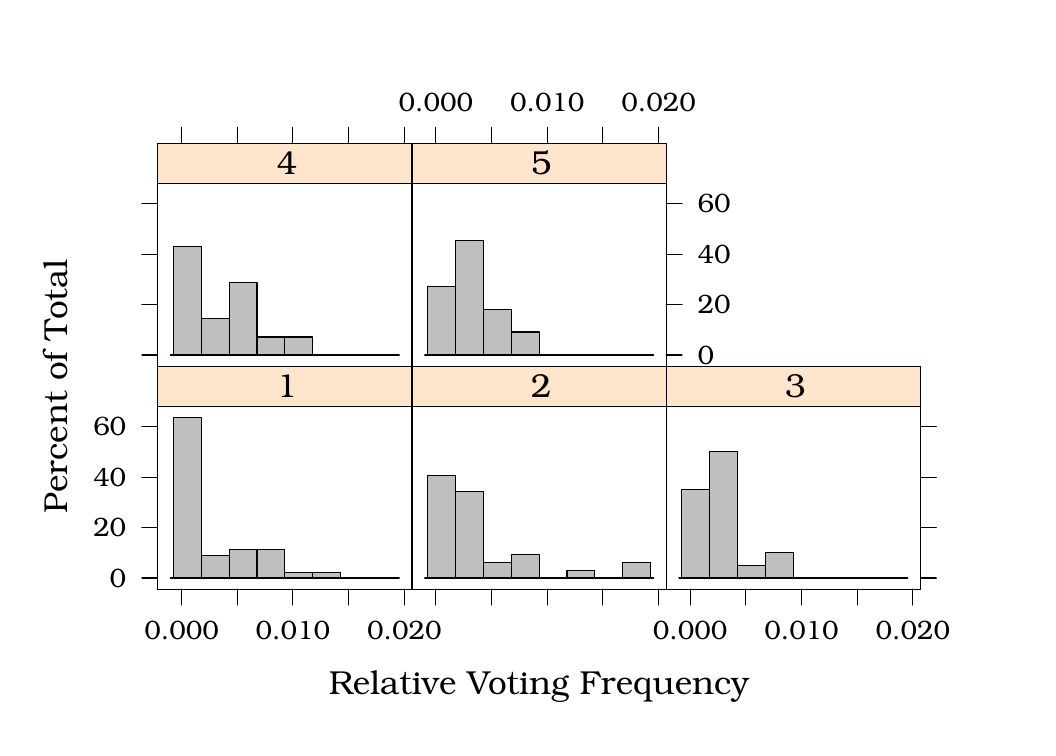
\begin{tikzpicture}[x=1pt,y=1pt]
\definecolor[named]{drawColor}{rgb}{0.00,0.00,0.00}
\definecolor[named]{fillColor}{rgb}{1.00,1.00,1.00}
\fill[color=fillColor,] (0,0) rectangle (361.35,252.94);
\begin{scope}
\path[clip] (  0.00,  0.00) rectangle (361.35,252.94);
\end{scope}
\begin{scope}
\path[clip] (  0.00,  0.00) rectangle (361.35,252.94);

\draw[fill opacity=0.00,draw opacity=0.00,] (  0.00,  0.00) rectangle (361.35,252.94);
\definecolor[named]{drawColor}{rgb}{0.00,0.00,0.00}

\node[color=drawColor,anchor=base,inner sep=0pt, outer sep=0pt, scale=  1.20] at (184.81, 12.04) {Relative Voting Frequency%
};
\end{scope}
\begin{scope}
\path[clip] (  0.00,  0.00) rectangle (361.35,252.94);
\definecolor[named]{drawColor}{rgb}{0.00,0.00,0.00}

\node[rotate= 90.00,color=drawColor,anchor=base,inner sep=0pt, outer sep=0pt, scale=  1.20] at ( 14.29,123.38) {Percent of Total%
};
\end{scope}
\begin{scope}
\path[clip] (  0.00,  0.00) rectangle (361.35,252.94);
\end{scope}
\begin{scope}
\path[clip] (  0.00,  0.00) rectangle (361.35,252.94);
\end{scope}
\begin{scope}
\path[clip] (  0.00,  0.00) rectangle (361.35,252.94);
\end{scope}
\begin{scope}
\path[clip] ( 46.98, 50.02) rectangle (138.86,116.15);
\end{scope}
\begin{scope}
\path[clip] (  0.00,  0.00) rectangle (361.35,252.94);
\end{scope}
\begin{scope}
\path[clip] (  0.00,  0.00) rectangle (361.35,252.94);
\end{scope}
\begin{scope}
\path[clip] (  0.00,  0.00) rectangle (361.35,252.94);
\end{scope}
\begin{scope}
\path[clip] (  0.00,  0.00) rectangle (361.35,252.94);
\definecolor[named]{drawColor}{rgb}{0.00,0.00,0.00}

\draw[color=drawColor,line cap=round,line join=round,fill opacity=0.00,] ( 46.98, 54.08) -- ( 41.29, 54.08);

\draw[color=drawColor,line cap=round,line join=round,fill opacity=0.00,] ( 46.98, 72.31) -- ( 41.29, 72.31);

\draw[color=drawColor,line cap=round,line join=round,fill opacity=0.00,] ( 46.98, 90.54) -- ( 41.29, 90.54);

\draw[color=drawColor,line cap=round,line join=round,fill opacity=0.00,] ( 46.98,108.77) -- ( 41.29,108.77);

\node[color=drawColor,anchor=base east,inner sep=0pt, outer sep=0pt, scale=  0.96] at ( 35.60, 50.77) {0%
};

\node[color=drawColor,anchor=base east,inner sep=0pt, outer sep=0pt, scale=  0.96] at ( 35.60, 69.00) {20%
};

\node[color=drawColor,anchor=base east,inner sep=0pt, outer sep=0pt, scale=  0.96] at ( 35.60, 87.24) {40%
};

\node[color=drawColor,anchor=base east,inner sep=0pt, outer sep=0pt, scale=  0.96] at ( 35.60,105.47) {60%
};
\end{scope}
\begin{scope}
\path[clip] (  0.00,  0.00) rectangle (361.35,252.94);
\end{scope}
\begin{scope}
\path[clip] (  0.00,  0.00) rectangle (361.35,252.94);
\definecolor[named]{drawColor}{rgb}{0.00,0.00,0.00}

\draw[color=drawColor,line cap=round,line join=round,fill opacity=0.00,] ( 55.61, 50.02) -- ( 55.61, 44.32);

\draw[color=drawColor,line cap=round,line join=round,fill opacity=0.00,] ( 75.73, 50.02) -- ( 75.73, 44.32);

\draw[color=drawColor,line cap=round,line join=round,fill opacity=0.00,] ( 95.85, 50.02) -- ( 95.85, 44.32);

\draw[color=drawColor,line cap=round,line join=round,fill opacity=0.00,] (115.98, 50.02) -- (115.98, 44.32);

\draw[color=drawColor,line cap=round,line join=round,fill opacity=0.00,] (136.10, 50.02) -- (136.10, 44.32);

\node[color=drawColor,anchor=base,inner sep=0pt, outer sep=0pt, scale=  0.96] at ( 55.61, 32.02) {0.000%
};

\node[color=drawColor,anchor=base,inner sep=0pt, outer sep=0pt, scale=  0.96] at ( 95.85, 32.02) {0.010%
};

\node[color=drawColor,anchor=base,inner sep=0pt, outer sep=0pt, scale=  0.96] at (136.10, 32.02) {0.020%
};
\end{scope}
\begin{scope}
\path[clip] (  0.00,  0.00) rectangle (361.35,252.94);
\end{scope}
\begin{scope}
\path[clip] ( 46.98, 50.02) rectangle (138.86,116.15);
\definecolor[named]{drawColor}{rgb}{0.00,0.00,0.00}

\draw[color=drawColor,line cap=round,line join=round,fill opacity=0.00,] ( 51.57, 54.08) --
	(134.27, 54.08);
\definecolor[named]{fillColor}{rgb}{0.75,0.75,0.75}

\draw[color=drawColor,line cap=round,line join=round,fill=fillColor,] ( 52.62, 54.08) rectangle ( 62.70,112.09);

\draw[color=drawColor,line cap=round,line join=round,fill=fillColor,] ( 62.70, 54.08) rectangle ( 72.77, 62.36);

\draw[color=drawColor,line cap=round,line join=round,fill=fillColor,] ( 72.77, 54.08) rectangle ( 82.85, 64.44);

\draw[color=drawColor,line cap=round,line join=round,fill=fillColor,] ( 82.85, 54.08) rectangle ( 92.92, 64.44);

\draw[color=drawColor,line cap=round,line join=round,fill=fillColor,] ( 92.92, 54.08) rectangle (103.00, 56.15);

\draw[color=drawColor,line cap=round,line join=round,fill=fillColor,] (103.00, 54.08) rectangle (113.07, 56.15);

\draw[color=drawColor,line cap=round,line join=round,fill=fillColor,] (113.07, 54.08) rectangle (123.15, 54.08);

\draw[color=drawColor,line cap=round,line join=round,fill=fillColor,] (123.15, 54.08) rectangle (133.22, 54.08);
\end{scope}
\begin{scope}
\path[clip] (  0.00,  0.00) rectangle (361.35,252.94);
\end{scope}
\begin{scope}
\path[clip] (  0.00,  0.00) rectangle (361.35,252.94);
\definecolor[named]{drawColor}{rgb}{0.00,0.00,0.00}

\draw[color=drawColor,line cap=round,line join=round,fill opacity=0.00,] ( 46.98, 50.02) rectangle (138.86,116.15);
\end{scope}
\begin{scope}
\path[clip] (  0.00,  0.00) rectangle (361.35,252.94);
\end{scope}
\begin{scope}
\path[clip] (  0.00,  0.00) rectangle (361.35,252.94);
\end{scope}
\begin{scope}
\path[clip] ( 46.98,116.15) rectangle (138.86,130.60);
\definecolor[named]{drawColor}{rgb}{1.00,0.90,0.80}
\definecolor[named]{fillColor}{rgb}{1.00,0.90,0.80}

\draw[color=drawColor,line cap=round,line join=round,fill=fillColor,] ( 46.98,116.15) rectangle (138.86,130.60);
\definecolor[named]{drawColor}{rgb}{0.00,0.00,0.00}

\node[color=drawColor,anchor=base west,inner sep=0pt, outer sep=0pt, scale=  1.20] at ( 89.92,119.25) {1%
};
\end{scope}
\begin{scope}
\path[clip] (  0.00,  0.00) rectangle (361.35,252.94);
\end{scope}
\begin{scope}
\path[clip] (  0.00,  0.00) rectangle (361.35,252.94);
\definecolor[named]{drawColor}{rgb}{0.00,0.00,0.00}

\draw[color=drawColor,line cap=round,line join=round,fill opacity=0.00,] ( 46.98,116.15) rectangle (138.86,130.60);
\end{scope}
\begin{scope}
\path[clip] (  0.00,  0.00) rectangle (361.35,252.94);
\end{scope}
\begin{scope}
\path[clip] (  0.00,  0.00) rectangle (361.35,252.94);
\end{scope}
\begin{scope}
\path[clip] (138.86, 50.02) rectangle (230.75,116.15);
\end{scope}
\begin{scope}
\path[clip] (  0.00,  0.00) rectangle (361.35,252.94);
\end{scope}
\begin{scope}
\path[clip] (  0.00,  0.00) rectangle (361.35,252.94);
\end{scope}
\begin{scope}
\path[clip] (  0.00,  0.00) rectangle (361.35,252.94);
\end{scope}
\begin{scope}
\path[clip] (  0.00,  0.00) rectangle (361.35,252.94);
\end{scope}
\begin{scope}
\path[clip] (  0.00,  0.00) rectangle (361.35,252.94);
\end{scope}
\begin{scope}
\path[clip] (  0.00,  0.00) rectangle (361.35,252.94);
\definecolor[named]{drawColor}{rgb}{0.00,0.00,0.00}

\draw[color=drawColor,line cap=round,line join=round,fill opacity=0.00,] (147.49, 50.02) -- (147.49, 44.32);

\draw[color=drawColor,line cap=round,line join=round,fill opacity=0.00,] (167.62, 50.02) -- (167.62, 44.32);

\draw[color=drawColor,line cap=round,line join=round,fill opacity=0.00,] (187.74, 50.02) -- (187.74, 44.32);

\draw[color=drawColor,line cap=round,line join=round,fill opacity=0.00,] (207.86, 50.02) -- (207.86, 44.32);

\draw[color=drawColor,line cap=round,line join=round,fill opacity=0.00,] (227.99, 50.02) -- (227.99, 44.32);
\end{scope}
\begin{scope}
\path[clip] (  0.00,  0.00) rectangle (361.35,252.94);
\end{scope}
\begin{scope}
\path[clip] (138.86, 50.02) rectangle (230.75,116.15);
\definecolor[named]{drawColor}{rgb}{0.00,0.00,0.00}

\draw[color=drawColor,line cap=round,line join=round,fill opacity=0.00,] (143.46, 54.08) --
	(226.16, 54.08);
\definecolor[named]{fillColor}{rgb}{0.75,0.75,0.75}

\draw[color=drawColor,line cap=round,line join=round,fill=fillColor,] (144.51, 54.08) rectangle (154.58, 91.11);

\draw[color=drawColor,line cap=round,line join=round,fill=fillColor,] (154.58, 54.08) rectangle (164.66, 85.41);

\draw[color=drawColor,line cap=round,line join=round,fill=fillColor,] (164.66, 54.08) rectangle (174.73, 59.77);

\draw[color=drawColor,line cap=round,line join=round,fill=fillColor,] (174.73, 54.08) rectangle (184.81, 62.62);

\draw[color=drawColor,line cap=round,line join=round,fill=fillColor,] (184.81, 54.08) rectangle (194.88, 54.08);

\draw[color=drawColor,line cap=round,line join=round,fill=fillColor,] (194.88, 54.08) rectangle (204.96, 56.93);

\draw[color=drawColor,line cap=round,line join=round,fill=fillColor,] (204.96, 54.08) rectangle (215.03, 54.08);

\draw[color=drawColor,line cap=round,line join=round,fill=fillColor,] (215.03, 54.08) rectangle (225.11, 59.77);
\end{scope}
\begin{scope}
\path[clip] (  0.00,  0.00) rectangle (361.35,252.94);
\end{scope}
\begin{scope}
\path[clip] (  0.00,  0.00) rectangle (361.35,252.94);
\definecolor[named]{drawColor}{rgb}{0.00,0.00,0.00}

\draw[color=drawColor,line cap=round,line join=round,fill opacity=0.00,] (138.86, 50.02) rectangle (230.75,116.15);
\end{scope}
\begin{scope}
\path[clip] (  0.00,  0.00) rectangle (361.35,252.94);
\end{scope}
\begin{scope}
\path[clip] (  0.00,  0.00) rectangle (361.35,252.94);
\end{scope}
\begin{scope}
\path[clip] (138.86,116.15) rectangle (230.75,130.60);
\definecolor[named]{drawColor}{rgb}{1.00,0.90,0.80}
\definecolor[named]{fillColor}{rgb}{1.00,0.90,0.80}

\draw[color=drawColor,line cap=round,line join=round,fill=fillColor,] (138.86,116.15) rectangle (230.75,130.60);
\definecolor[named]{drawColor}{rgb}{0.00,0.00,0.00}

\node[color=drawColor,anchor=base west,inner sep=0pt, outer sep=0pt, scale=  1.20] at (181.81,119.25) {2%
};
\end{scope}
\begin{scope}
\path[clip] (  0.00,  0.00) rectangle (361.35,252.94);
\end{scope}
\begin{scope}
\path[clip] (  0.00,  0.00) rectangle (361.35,252.94);
\definecolor[named]{drawColor}{rgb}{0.00,0.00,0.00}

\draw[color=drawColor,line cap=round,line join=round,fill opacity=0.00,] (138.86,116.15) rectangle (230.75,130.60);
\end{scope}
\begin{scope}
\path[clip] (  0.00,  0.00) rectangle (361.35,252.94);
\end{scope}
\begin{scope}
\path[clip] (  0.00,  0.00) rectangle (361.35,252.94);
\end{scope}
\begin{scope}
\path[clip] (230.75, 50.02) rectangle (322.64,116.15);
\end{scope}
\begin{scope}
\path[clip] (  0.00,  0.00) rectangle (361.35,252.94);
\end{scope}
\begin{scope}
\path[clip] (  0.00,  0.00) rectangle (361.35,252.94);
\end{scope}
\begin{scope}
\path[clip] (  0.00,  0.00) rectangle (361.35,252.94);
\end{scope}
\begin{scope}
\path[clip] (  0.00,  0.00) rectangle (361.35,252.94);
\end{scope}
\begin{scope}
\path[clip] (  0.00,  0.00) rectangle (361.35,252.94);
\end{scope}
\begin{scope}
\path[clip] (  0.00,  0.00) rectangle (361.35,252.94);
\definecolor[named]{drawColor}{rgb}{0.00,0.00,0.00}

\draw[color=drawColor,line cap=round,line join=round,fill opacity=0.00,] (239.38, 50.02) -- (239.38, 44.32);

\draw[color=drawColor,line cap=round,line join=round,fill opacity=0.00,] (259.50, 50.02) -- (259.50, 44.32);

\draw[color=drawColor,line cap=round,line join=round,fill opacity=0.00,] (279.62, 50.02) -- (279.62, 44.32);

\draw[color=drawColor,line cap=round,line join=round,fill opacity=0.00,] (299.75, 50.02) -- (299.75, 44.32);

\draw[color=drawColor,line cap=round,line join=round,fill opacity=0.00,] (319.87, 50.02) -- (319.87, 44.32);

\node[color=drawColor,anchor=base,inner sep=0pt, outer sep=0pt, scale=  0.96] at (239.38, 32.02) {0.000%
};

\node[color=drawColor,anchor=base,inner sep=0pt, outer sep=0pt, scale=  0.96] at (279.62, 32.02) {0.010%
};

\node[color=drawColor,anchor=base,inner sep=0pt, outer sep=0pt, scale=  0.96] at (319.87, 32.02) {0.020%
};

\draw[color=drawColor,line cap=round,line join=round,fill opacity=0.00,] (322.64, 54.08) -- (328.33, 54.08);

\draw[color=drawColor,line cap=round,line join=round,fill opacity=0.00,] (322.64, 72.31) -- (328.33, 72.31);

\draw[color=drawColor,line cap=round,line join=round,fill opacity=0.00,] (322.64, 90.54) -- (328.33, 90.54);

\draw[color=drawColor,line cap=round,line join=round,fill opacity=0.00,] (322.64,108.77) -- (328.33,108.77);
\end{scope}
\begin{scope}
\path[clip] (  0.00,  0.00) rectangle (361.35,252.94);
\end{scope}
\begin{scope}
\path[clip] (230.75, 50.02) rectangle (322.64,116.15);
\definecolor[named]{drawColor}{rgb}{0.00,0.00,0.00}

\draw[color=drawColor,line cap=round,line join=round,fill opacity=0.00,] (235.34, 54.08) --
	(318.04, 54.08);
\definecolor[named]{fillColor}{rgb}{0.75,0.75,0.75}

\draw[color=drawColor,line cap=round,line join=round,fill=fillColor,] (236.39, 54.08) rectangle (246.47, 85.98);

\draw[color=drawColor,line cap=round,line join=round,fill=fillColor,] (246.47, 54.08) rectangle (256.54, 99.66);

\draw[color=drawColor,line cap=round,line join=round,fill=fillColor,] (256.54, 54.08) rectangle (266.62, 58.63);

\draw[color=drawColor,line cap=round,line join=round,fill=fillColor,] (266.62, 54.08) rectangle (276.69, 63.19);

\draw[color=drawColor,line cap=round,line join=round,fill=fillColor,] (276.69, 54.08) rectangle (286.77, 54.08);

\draw[color=drawColor,line cap=round,line join=round,fill=fillColor,] (286.77, 54.08) rectangle (296.84, 54.08);

\draw[color=drawColor,line cap=round,line join=round,fill=fillColor,] (296.84, 54.08) rectangle (306.92, 54.08);

\draw[color=drawColor,line cap=round,line join=round,fill=fillColor,] (306.92, 54.08) rectangle (316.99, 54.08);
\end{scope}
\begin{scope}
\path[clip] (  0.00,  0.00) rectangle (361.35,252.94);
\end{scope}
\begin{scope}
\path[clip] (  0.00,  0.00) rectangle (361.35,252.94);
\definecolor[named]{drawColor}{rgb}{0.00,0.00,0.00}

\draw[color=drawColor,line cap=round,line join=round,fill opacity=0.00,] (230.75, 50.02) rectangle (322.64,116.15);
\end{scope}
\begin{scope}
\path[clip] (  0.00,  0.00) rectangle (361.35,252.94);
\end{scope}
\begin{scope}
\path[clip] (  0.00,  0.00) rectangle (361.35,252.94);
\end{scope}
\begin{scope}
\path[clip] (230.75,116.15) rectangle (322.64,130.60);
\definecolor[named]{drawColor}{rgb}{1.00,0.90,0.80}
\definecolor[named]{fillColor}{rgb}{1.00,0.90,0.80}

\draw[color=drawColor,line cap=round,line join=round,fill=fillColor,] (230.75,116.15) rectangle (322.64,130.60);
\definecolor[named]{drawColor}{rgb}{0.00,0.00,0.00}

\node[color=drawColor,anchor=base west,inner sep=0pt, outer sep=0pt, scale=  1.20] at (273.69,119.25) {3%
};
\end{scope}
\begin{scope}
\path[clip] (  0.00,  0.00) rectangle (361.35,252.94);
\end{scope}
\begin{scope}
\path[clip] (  0.00,  0.00) rectangle (361.35,252.94);
\definecolor[named]{drawColor}{rgb}{0.00,0.00,0.00}

\draw[color=drawColor,line cap=round,line join=round,fill opacity=0.00,] (230.75,116.15) rectangle (322.64,130.60);
\end{scope}
\begin{scope}
\path[clip] (  0.00,  0.00) rectangle (361.35,252.94);
\end{scope}
\begin{scope}
\path[clip] (  0.00,  0.00) rectangle (361.35,252.94);
\end{scope}
\begin{scope}
\path[clip] ( 46.98,130.60) rectangle (138.86,196.74);
\end{scope}
\begin{scope}
\path[clip] (  0.00,  0.00) rectangle (361.35,252.94);
\end{scope}
\begin{scope}
\path[clip] (  0.00,  0.00) rectangle (361.35,252.94);
\definecolor[named]{drawColor}{rgb}{0.00,0.00,0.00}

\draw[color=drawColor,line cap=round,line join=round,fill opacity=0.00,] ( 55.61,211.19) -- ( 55.61,216.88);

\draw[color=drawColor,line cap=round,line join=round,fill opacity=0.00,] ( 75.73,211.19) -- ( 75.73,216.88);

\draw[color=drawColor,line cap=round,line join=round,fill opacity=0.00,] ( 95.85,211.19) -- ( 95.85,216.88);

\draw[color=drawColor,line cap=round,line join=round,fill opacity=0.00,] (115.98,211.19) -- (115.98,216.88);

\draw[color=drawColor,line cap=round,line join=round,fill opacity=0.00,] (136.10,211.19) -- (136.10,216.88);
\end{scope}
\begin{scope}
\path[clip] (  0.00,  0.00) rectangle (361.35,252.94);
\end{scope}
\begin{scope}
\path[clip] (  0.00,  0.00) rectangle (361.35,252.94);
\definecolor[named]{drawColor}{rgb}{0.00,0.00,0.00}

\draw[color=drawColor,line cap=round,line join=round,fill opacity=0.00,] ( 46.98,134.67) -- ( 41.29,134.67);

\draw[color=drawColor,line cap=round,line join=round,fill opacity=0.00,] ( 46.98,152.90) -- ( 41.29,152.90);

\draw[color=drawColor,line cap=round,line join=round,fill opacity=0.00,] ( 46.98,171.13) -- ( 41.29,171.13);

\draw[color=drawColor,line cap=round,line join=round,fill opacity=0.00,] ( 46.98,189.36) -- ( 41.29,189.36);
\end{scope}
\begin{scope}
\path[clip] (  0.00,  0.00) rectangle (361.35,252.94);
\end{scope}
\begin{scope}
\path[clip] (  0.00,  0.00) rectangle (361.35,252.94);
\end{scope}
\begin{scope}
\path[clip] (  0.00,  0.00) rectangle (361.35,252.94);
\end{scope}
\begin{scope}
\path[clip] ( 46.98,130.60) rectangle (138.86,196.74);
\definecolor[named]{drawColor}{rgb}{0.00,0.00,0.00}

\draw[color=drawColor,line cap=round,line join=round,fill opacity=0.00,] ( 51.57,134.67) --
	(134.27,134.67);
\definecolor[named]{fillColor}{rgb}{0.75,0.75,0.75}

\draw[color=drawColor,line cap=round,line join=round,fill=fillColor,] ( 52.62,134.67) rectangle ( 62.70,173.74);

\draw[color=drawColor,line cap=round,line join=round,fill=fillColor,] ( 62.70,134.67) rectangle ( 72.77,147.69);

\draw[color=drawColor,line cap=round,line join=round,fill=fillColor,] ( 72.77,134.67) rectangle ( 82.85,160.71);

\draw[color=drawColor,line cap=round,line join=round,fill=fillColor,] ( 82.85,134.67) rectangle ( 92.92,141.18);

\draw[color=drawColor,line cap=round,line join=round,fill=fillColor,] ( 92.92,134.67) rectangle (103.00,141.18);

\draw[color=drawColor,line cap=round,line join=round,fill=fillColor,] (103.00,134.67) rectangle (113.07,134.67);

\draw[color=drawColor,line cap=round,line join=round,fill=fillColor,] (113.07,134.67) rectangle (123.15,134.67);

\draw[color=drawColor,line cap=round,line join=round,fill=fillColor,] (123.15,134.67) rectangle (133.22,134.67);
\end{scope}
\begin{scope}
\path[clip] (  0.00,  0.00) rectangle (361.35,252.94);
\end{scope}
\begin{scope}
\path[clip] (  0.00,  0.00) rectangle (361.35,252.94);
\definecolor[named]{drawColor}{rgb}{0.00,0.00,0.00}

\draw[color=drawColor,line cap=round,line join=round,fill opacity=0.00,] ( 46.98,130.60) rectangle (138.86,196.74);
\end{scope}
\begin{scope}
\path[clip] (  0.00,  0.00) rectangle (361.35,252.94);
\end{scope}
\begin{scope}
\path[clip] (  0.00,  0.00) rectangle (361.35,252.94);
\end{scope}
\begin{scope}
\path[clip] ( 46.98,196.74) rectangle (138.86,211.19);
\definecolor[named]{drawColor}{rgb}{1.00,0.90,0.80}
\definecolor[named]{fillColor}{rgb}{1.00,0.90,0.80}

\draw[color=drawColor,line cap=round,line join=round,fill=fillColor,] ( 46.98,196.74) rectangle (138.86,211.19);
\definecolor[named]{drawColor}{rgb}{0.00,0.00,0.00}

\node[color=drawColor,anchor=base west,inner sep=0pt, outer sep=0pt, scale=  1.20] at ( 89.92,199.83) {4%
};
\end{scope}
\begin{scope}
\path[clip] (  0.00,  0.00) rectangle (361.35,252.94);
\end{scope}
\begin{scope}
\path[clip] (  0.00,  0.00) rectangle (361.35,252.94);
\definecolor[named]{drawColor}{rgb}{0.00,0.00,0.00}

\draw[color=drawColor,line cap=round,line join=round,fill opacity=0.00,] ( 46.98,196.74) rectangle (138.86,211.19);
\end{scope}
\begin{scope}
\path[clip] (  0.00,  0.00) rectangle (361.35,252.94);
\end{scope}
\begin{scope}
\path[clip] (  0.00,  0.00) rectangle (361.35,252.94);
\end{scope}
\begin{scope}
\path[clip] (138.86,130.60) rectangle (230.75,196.74);
\end{scope}
\begin{scope}
\path[clip] (  0.00,  0.00) rectangle (361.35,252.94);
\end{scope}
\begin{scope}
\path[clip] (  0.00,  0.00) rectangle (361.35,252.94);
\definecolor[named]{drawColor}{rgb}{0.00,0.00,0.00}

\draw[color=drawColor,line cap=round,line join=round,fill opacity=0.00,] (147.49,211.19) -- (147.49,216.88);

\draw[color=drawColor,line cap=round,line join=round,fill opacity=0.00,] (167.62,211.19) -- (167.62,216.88);

\draw[color=drawColor,line cap=round,line join=round,fill opacity=0.00,] (187.74,211.19) -- (187.74,216.88);

\draw[color=drawColor,line cap=round,line join=round,fill opacity=0.00,] (207.86,211.19) -- (207.86,216.88);

\draw[color=drawColor,line cap=round,line join=round,fill opacity=0.00,] (227.99,211.19) -- (227.99,216.88);

\node[color=drawColor,anchor=base,inner sep=0pt, outer sep=0pt, scale=  0.96] at (147.49,222.58) {0.000%
};

\node[color=drawColor,anchor=base,inner sep=0pt, outer sep=0pt, scale=  0.96] at (187.74,222.58) {0.010%
};

\node[color=drawColor,anchor=base,inner sep=0pt, outer sep=0pt, scale=  0.96] at (227.99,222.58) {0.020%
};
\end{scope}
\begin{scope}
\path[clip] (  0.00,  0.00) rectangle (361.35,252.94);
\end{scope}
\begin{scope}
\path[clip] (  0.00,  0.00) rectangle (361.35,252.94);
\end{scope}
\begin{scope}
\path[clip] (  0.00,  0.00) rectangle (361.35,252.94);
\end{scope}
\begin{scope}
\path[clip] (  0.00,  0.00) rectangle (361.35,252.94);
\definecolor[named]{drawColor}{rgb}{0.00,0.00,0.00}

\draw[color=drawColor,line cap=round,line join=round,fill opacity=0.00,] (230.75,134.67) -- (236.44,134.67);

\draw[color=drawColor,line cap=round,line join=round,fill opacity=0.00,] (230.75,152.90) -- (236.44,152.90);

\draw[color=drawColor,line cap=round,line join=round,fill opacity=0.00,] (230.75,171.13) -- (236.44,171.13);

\draw[color=drawColor,line cap=round,line join=round,fill opacity=0.00,] (230.75,189.36) -- (236.44,189.36);

\node[color=drawColor,anchor=base west,inner sep=0pt, outer sep=0pt, scale=  0.96] at (242.13,131.36) {0%
};

\node[color=drawColor,anchor=base west,inner sep=0pt, outer sep=0pt, scale=  0.96] at (242.13,149.59) {20%
};

\node[color=drawColor,anchor=base west,inner sep=0pt, outer sep=0pt, scale=  0.96] at (242.13,167.83) {40%
};

\node[color=drawColor,anchor=base west,inner sep=0pt, outer sep=0pt, scale=  0.96] at (242.13,186.06) {60%
};
\end{scope}
\begin{scope}
\path[clip] (  0.00,  0.00) rectangle (361.35,252.94);
\end{scope}
\begin{scope}
\path[clip] (138.86,130.60) rectangle (230.75,196.74);
\definecolor[named]{drawColor}{rgb}{0.00,0.00,0.00}

\draw[color=drawColor,line cap=round,line join=round,fill opacity=0.00,] (143.46,134.67) --
	(226.16,134.67);
\definecolor[named]{fillColor}{rgb}{0.75,0.75,0.75}

\draw[color=drawColor,line cap=round,line join=round,fill=fillColor,] (144.51,134.67) rectangle (154.58,159.53);

\draw[color=drawColor,line cap=round,line join=round,fill=fillColor,] (154.58,134.67) rectangle (164.66,176.10);

\draw[color=drawColor,line cap=round,line join=round,fill=fillColor,] (164.66,134.67) rectangle (174.73,151.24);

\draw[color=drawColor,line cap=round,line join=round,fill=fillColor,] (174.73,134.67) rectangle (184.81,142.95);

\draw[color=drawColor,line cap=round,line join=round,fill=fillColor,] (184.81,134.67) rectangle (194.88,134.67);

\draw[color=drawColor,line cap=round,line join=round,fill=fillColor,] (194.88,134.67) rectangle (204.96,134.67);

\draw[color=drawColor,line cap=round,line join=round,fill=fillColor,] (204.96,134.67) rectangle (215.03,134.67);

\draw[color=drawColor,line cap=round,line join=round,fill=fillColor,] (215.03,134.67) rectangle (225.11,134.67);
\end{scope}
\begin{scope}
\path[clip] (  0.00,  0.00) rectangle (361.35,252.94);
\end{scope}
\begin{scope}
\path[clip] (  0.00,  0.00) rectangle (361.35,252.94);
\definecolor[named]{drawColor}{rgb}{0.00,0.00,0.00}

\draw[color=drawColor,line cap=round,line join=round,fill opacity=0.00,] (138.86,130.60) rectangle (230.75,196.74);
\end{scope}
\begin{scope}
\path[clip] (  0.00,  0.00) rectangle (361.35,252.94);
\end{scope}
\begin{scope}
\path[clip] (  0.00,  0.00) rectangle (361.35,252.94);
\end{scope}
\begin{scope}
\path[clip] (138.86,196.74) rectangle (230.75,211.19);
\definecolor[named]{drawColor}{rgb}{1.00,0.90,0.80}
\definecolor[named]{fillColor}{rgb}{1.00,0.90,0.80}

\draw[color=drawColor,line cap=round,line join=round,fill=fillColor,] (138.86,196.74) rectangle (230.75,211.19);
\definecolor[named]{drawColor}{rgb}{0.00,0.00,0.00}

\node[color=drawColor,anchor=base west,inner sep=0pt, outer sep=0pt, scale=  1.20] at (181.81,199.83) {5%
};
\end{scope}
\begin{scope}
\path[clip] (  0.00,  0.00) rectangle (361.35,252.94);
\end{scope}
\begin{scope}
\path[clip] (  0.00,  0.00) rectangle (361.35,252.94);
\definecolor[named]{drawColor}{rgb}{0.00,0.00,0.00}

\draw[color=drawColor,line cap=round,line join=round,fill opacity=0.00,] (138.86,196.74) rectangle (230.75,211.19);
\end{scope}
\begin{scope}
\path[clip] (  0.00,  0.00) rectangle (361.35,252.94);
\end{scope}
\begin{scope}
\path[clip] (  0.00,  0.00) rectangle (361.35,252.94);
\end{scope}
\begin{scope}
\path[clip] (  0.00,  0.00) rectangle (361.35,252.94);
\end{scope}
\begin{scope}
\path[clip] (  0.00,  0.00) rectangle (361.35,252.94);
\end{scope}
\end{tikzpicture}
}}\quad
\caption{The plots show the conditional distribtion of relative voting frequencies within each time category.}
\label{fig:histogram}
\end{figure}

The important aspect to notice in Figure \ref{fig:histogram} is that for the no votes, conditioning on meeting frequency does not change the distribution in any significant way. The choice to cast a no vote is independent of the time spend in the Council. This corroborates the thesis that no votes are signaling devices aimed at domestic audiences, as the interest of domestic audiences in the dossiers coming from the Commission are independent of time. For abstentions and yes votes with a dissenting statement we see that the number of governments that has not cast a vote in this category decrease as time passes, lending partial corroborating evidence for hypothesis three.




\section{Inferential Analysis}
In order to further test the hypotheses we turn to statistical modeling. The dependent variable is the vote choice of the individual government, since it is difficult to rank the variable a multinomial logisitc choice model is appropriate. These models are suitable first and foremost as they do not make any assumptions about the ordinality of a variable, furthermore they do not make any assumption about normality, linearity and homogeneity of variance of the independent variables. Thus these models represent a very flexible modeling framework when dealing with choice categories. However there are two crucial assumptions made in these models which must be justified. The first assumption is commonly labelled independence of irrelevant alternatives (IIA). This assumes that the results from the analysis would not change if we threw in another choice category which would clearly be irrelevant to the problem being modeled. The classic example is the study of modes of transport. If subjects has to make a choice between taking the bus, ride a bike or taking the car to work, then the results from such an analysis should not change if we added two bus categories, one with red busses and one with blue busses. Since the color coding of busses should be irrelevant we would expect the subjects to randomly choose between the two busses. 


The overall pattern that emerges from the models is one where receiving more from the EU than you give, and being powerful reduces dissenting behavior, whereas being a preference outlier decreases the number of yes votes, however the number of yes votes with a dissenting statement increases substantially. The first two effects can be explained by classic rational-institutionalist mechanisms, however the last effect is not so straightforward. From a rational-institutionalist perspective sending conflicting signals (voting yes, but saying no) is meaningful in signaling games where the players are trying to outsmart each other. In the present context the statement is attached after the vote, so it could not have been part of a bargaining strategy. From a logrolling perspective the behavior is also puzzling. There is no reason for an actor after a deal has been done, to then publicly state his/her opposition to this deal while still supporting it. From a logrolling perspective, once a deal has been done its done \citep{Warntjen2010}. From the perspective of diffuse reciprocity, such behavior makes more sense. Signaling do not necessarily have to be towards a well defined opponent, as the rational choice signaling games assume, but could also be aimed at future negotiations with the same partners. This notion of signaling to a future, unknown, negotiation, is only possible when a level of trust and reciprocity has been created in a group. This has been amply documented to be the case in the Council. Furthermore \citet{ElgstromJonsson2000} has shown that this type of behavior is consistent with a problem-solving style of bargaining, where there is a long shadow of the future. Hence the results reported here provide further support for the statement by Elgstrom and Jonnson, that the council is made up of:

\begin{quote}
  ``[...] a predominant problem-solving approavh with islands of conflictual bargaining.
\flushright{- \citealt[p. 697]{ElgstromJonsson2000}}
\end{quote}

\section{Conclusion}

In this paper a new data set was used which merged data from the PreLex data base and the Council monthly summaries. This allowed us to select cases that all had an element of conflict in them, based on the fact that non-controversial dossiers do not contain any meaningful information when studying decision making in the Council. The data was then disaggregated into each vote for each government in each member state of the EU. This allowed the use of a multinomial logit model to model the vote choice of the individual government. The implication being that studies who only focuses on member states risk biasing their analysis as governments change. That different governments from the same member state can differ a lot was witnessed in table \ref{tab:dissent}, where the Schroeder II government was among the ten most dissenting government in the EU in the 1999 - 2009 period, wheres the Merkel governments did not come close to the top. The explanation lies in the fact that the preference composition of the Council changes over time as old governments leave office and new governments enter office. Thus the Schroeder II government found itself an outlier in the Council (an average absolute deviation of 2.46 over its duration). The effect of being an outlier does not only lead to an increase in no votes and abstentions, but also to a substantial increase in dissenting statements attached to yes votes. An increase that is much more pronounced than the increase in no votes and abstentions. This type of behavior is difficult to reconcile with either a pure rational-institutionalist argument or a pure constructivist argument. In stead the answer is complex and lies between the two poles. Governments engage in both bargaining and problem-solving, however from af frequency point of view problem-solving is dominant. The fact that the main variable supposed to capture the effect of socialization did not show any effect, whereas the classic rational-institutionalist variables where significant, but had effects that where not predicted by the theory provides several points worthy of mentioning. First of all, the proxy for socialization was most likely a bad proxy, so it can be argued whether this paper successfully managed to find the pure rational-institutionalist effect of the outlier variable. This would explain the differentiated effects of the outlier variable. This, however, raises another point. Since a large part of the effect of the outlier variable was in an area of the dependent variable not measured in other studies, papers only using classic rational-institutionalist variables , without controlling for socialization effects, risks introducing bias into their models. 


\section{Appendix}

%\begin{sidewaysfigure}[htp]
%\centering
%\scalebox{.5}{\subfloat[][]{% Created by tikzDevice version 0.6.1 on 2011-08-03 09:51:04
% !TEX encoding = UTF-8 Unicode
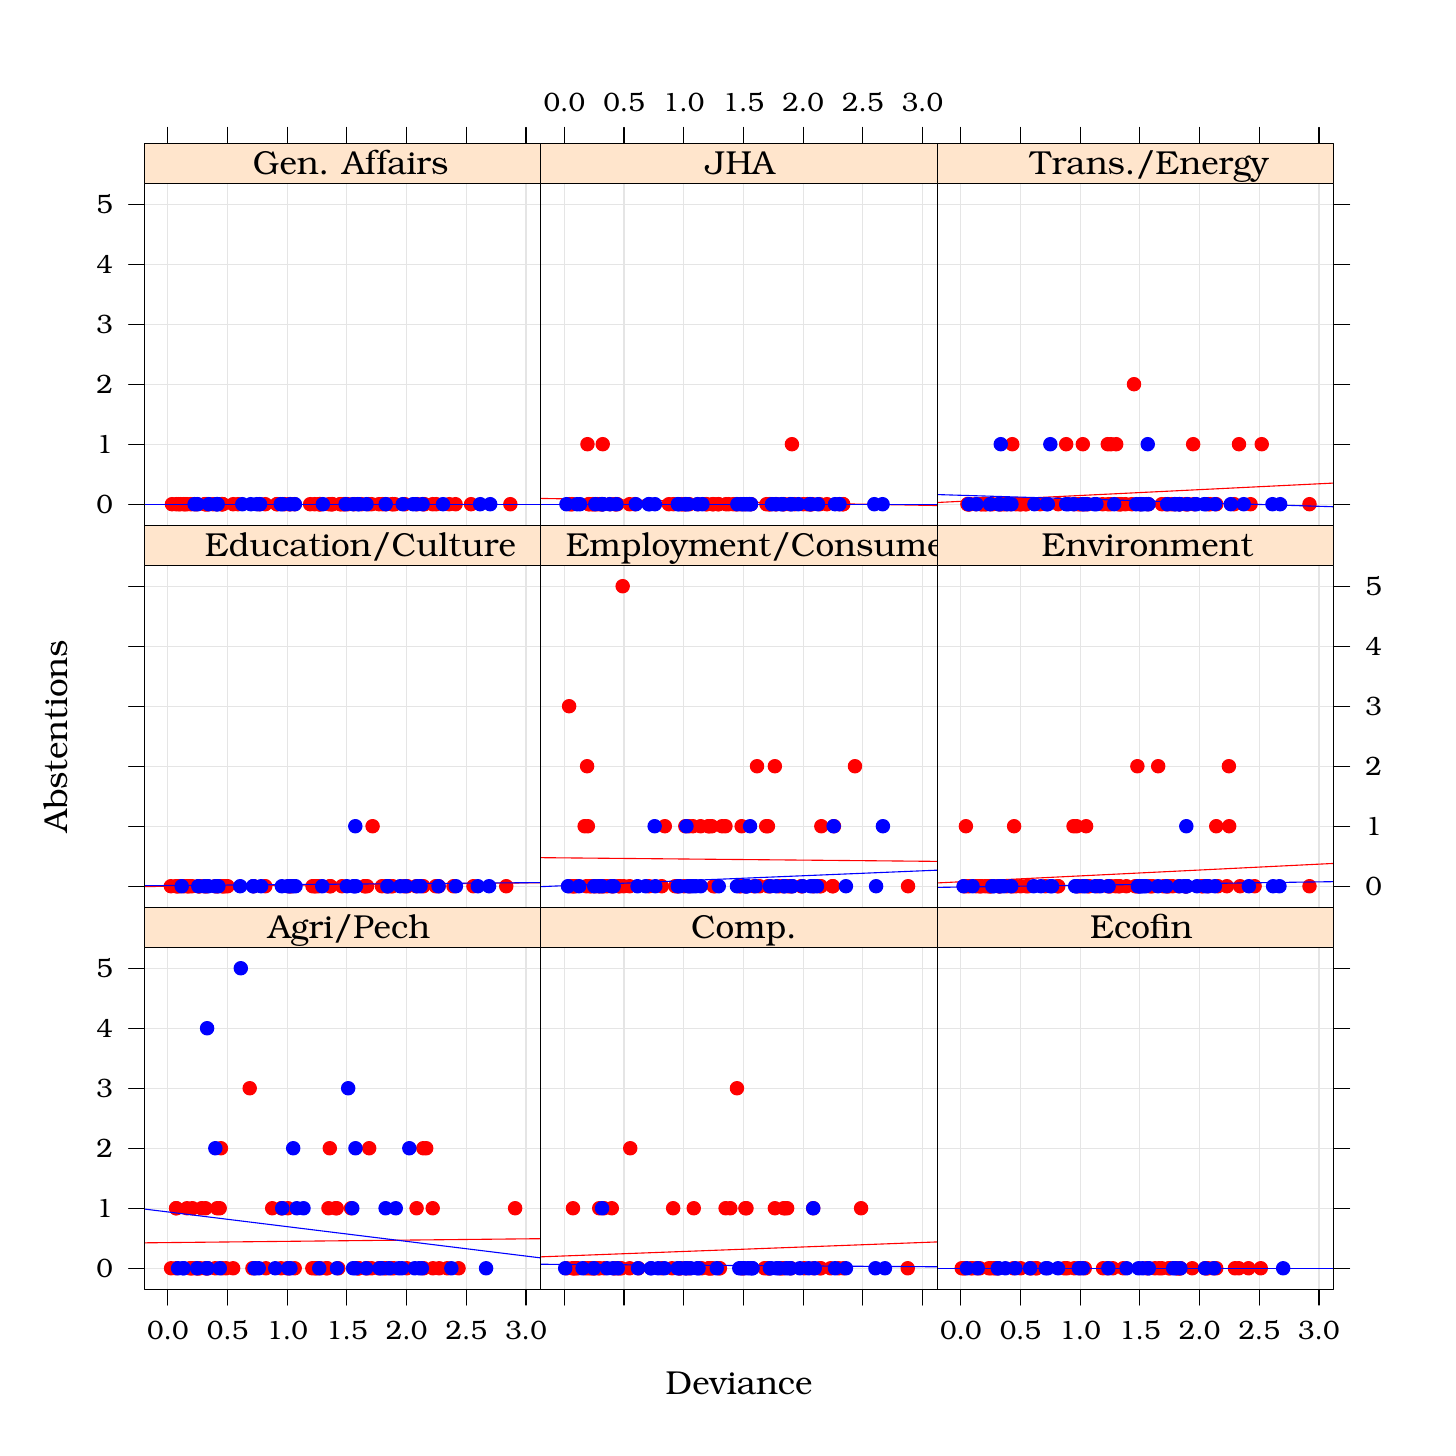
\begin{tikzpicture}[x=1pt,y=1pt]
\definecolor[named]{drawColor}{rgb}{0.00,0.00,0.00}
\definecolor[named]{fillColor}{rgb}{1.00,1.00,1.00}
\fill[color=fillColor,] (0,0) rectangle (505.89,505.89);
\begin{scope}
\path[clip] (  0.00,  0.00) rectangle (505.89,505.89);
\definecolor[named]{fillColor}{rgb}{0.00,0.00,0.00}
\end{scope}
\begin{scope}
\path[clip] (  0.00,  0.00) rectangle (505.89,505.89);
\definecolor[named]{fillColor}{rgb}{0.00,0.00,0.00}

\draw[fill opacity=0.00,draw opacity=0.00,] (  0.00,  0.00) rectangle (505.89,505.89);
\definecolor[named]{drawColor}{rgb}{0.00,0.00,0.00}

\node[color=drawColor,anchor=base,inner sep=0pt, outer sep=0pt, scale=  1.20] at (257.08, 12.04) {Deviance%
};
\end{scope}
\begin{scope}
\path[clip] (  0.00,  0.00) rectangle (505.89,505.89);
\definecolor[named]{fillColor}{rgb}{0.00,0.00,0.00}
\definecolor[named]{drawColor}{rgb}{0.00,0.00,0.00}

\node[rotate= 90.00,color=drawColor,anchor=base,inner sep=0pt, outer sep=0pt, scale=  1.20] at ( 14.29,249.85) {Abstentions%
};
\end{scope}
\begin{scope}
\path[clip] (  0.00,  0.00) rectangle (505.89,505.89);
\definecolor[named]{fillColor}{rgb}{0.00,0.00,0.00}
\end{scope}
\begin{scope}
\path[clip] (  0.00,  0.00) rectangle (505.89,505.89);
\definecolor[named]{fillColor}{rgb}{0.00,0.00,0.00}
\end{scope}
\begin{scope}
\path[clip] (  0.00,  0.00) rectangle (505.89,505.89);
\definecolor[named]{fillColor}{rgb}{0.00,0.00,0.00}
\end{scope}
\begin{scope}
\path[clip] ( 42.18, 50.02) rectangle (185.44,173.60);
\definecolor[named]{fillColor}{rgb}{0.00,0.00,0.00}
\end{scope}
\begin{scope}
\path[clip] (  0.00,  0.00) rectangle (505.89,505.89);
\definecolor[named]{fillColor}{rgb}{0.00,0.00,0.00}
\end{scope}
\begin{scope}
\path[clip] (  0.00,  0.00) rectangle (505.89,505.89);
\definecolor[named]{fillColor}{rgb}{0.00,0.00,0.00}
\end{scope}
\begin{scope}
\path[clip] (  0.00,  0.00) rectangle (505.89,505.89);
\definecolor[named]{fillColor}{rgb}{0.00,0.00,0.00}
\end{scope}
\begin{scope}
\path[clip] (  0.00,  0.00) rectangle (505.89,505.89);
\definecolor[named]{fillColor}{rgb}{0.00,0.00,0.00}
\definecolor[named]{drawColor}{rgb}{0.00,0.00,0.00}

\draw[color=drawColor,line cap=round,line join=round,fill opacity=0.00,] ( 42.18, 57.60) -- ( 36.49, 57.60);

\draw[color=drawColor,line cap=round,line join=round,fill opacity=0.00,] ( 42.18, 79.29) -- ( 36.49, 79.29);

\draw[color=drawColor,line cap=round,line join=round,fill opacity=0.00,] ( 42.18,100.97) -- ( 36.49,100.97);

\draw[color=drawColor,line cap=round,line join=round,fill opacity=0.00,] ( 42.18,122.65) -- ( 36.49,122.65);

\draw[color=drawColor,line cap=round,line join=round,fill opacity=0.00,] ( 42.18,144.33) -- ( 36.49,144.33);

\draw[color=drawColor,line cap=round,line join=round,fill opacity=0.00,] ( 42.18,166.01) -- ( 36.49,166.01);

\node[color=drawColor,anchor=base east,inner sep=0pt, outer sep=0pt, scale=  0.96] at ( 30.80, 54.30) {0%
};

\node[color=drawColor,anchor=base east,inner sep=0pt, outer sep=0pt, scale=  0.96] at ( 30.80, 75.98) {1%
};

\node[color=drawColor,anchor=base east,inner sep=0pt, outer sep=0pt, scale=  0.96] at ( 30.80, 97.66) {2%
};

\node[color=drawColor,anchor=base east,inner sep=0pt, outer sep=0pt, scale=  0.96] at ( 30.80,119.34) {3%
};

\node[color=drawColor,anchor=base east,inner sep=0pt, outer sep=0pt, scale=  0.96] at ( 30.80,141.03) {4%
};

\node[color=drawColor,anchor=base east,inner sep=0pt, outer sep=0pt, scale=  0.96] at ( 30.80,162.71) {5%
};
\end{scope}
\begin{scope}
\path[clip] (  0.00,  0.00) rectangle (505.89,505.89);
\definecolor[named]{fillColor}{rgb}{0.00,0.00,0.00}
\end{scope}
\begin{scope}
\path[clip] (  0.00,  0.00) rectangle (505.89,505.89);
\definecolor[named]{fillColor}{rgb}{0.00,0.00,0.00}
\definecolor[named]{drawColor}{rgb}{0.00,0.00,0.00}

\draw[color=drawColor,line cap=round,line join=round,fill opacity=0.00,] ( 50.65, 50.02) -- ( 50.65, 44.32);

\draw[color=drawColor,line cap=round,line join=round,fill opacity=0.00,] ( 72.22, 50.02) -- ( 72.22, 44.32);

\draw[color=drawColor,line cap=round,line join=round,fill opacity=0.00,] ( 93.79, 50.02) -- ( 93.79, 44.32);

\draw[color=drawColor,line cap=round,line join=round,fill opacity=0.00,] (115.36, 50.02) -- (115.36, 44.32);

\draw[color=drawColor,line cap=round,line join=round,fill opacity=0.00,] (136.93, 50.02) -- (136.93, 44.32);

\draw[color=drawColor,line cap=round,line join=round,fill opacity=0.00,] (158.50, 50.02) -- (158.50, 44.32);

\draw[color=drawColor,line cap=round,line join=round,fill opacity=0.00,] (180.07, 50.02) -- (180.07, 44.32);

\node[color=drawColor,anchor=base,inner sep=0pt, outer sep=0pt, scale=  0.96] at ( 50.65, 32.02) {0.0%
};

\node[color=drawColor,anchor=base,inner sep=0pt, outer sep=0pt, scale=  0.96] at ( 72.22, 32.02) {0.5%
};

\node[color=drawColor,anchor=base,inner sep=0pt, outer sep=0pt, scale=  0.96] at ( 93.79, 32.02) {1.0%
};

\node[color=drawColor,anchor=base,inner sep=0pt, outer sep=0pt, scale=  0.96] at (115.36, 32.02) {1.5%
};

\node[color=drawColor,anchor=base,inner sep=0pt, outer sep=0pt, scale=  0.96] at (136.93, 32.02) {2.0%
};

\node[color=drawColor,anchor=base,inner sep=0pt, outer sep=0pt, scale=  0.96] at (158.50, 32.02) {2.5%
};

\node[color=drawColor,anchor=base,inner sep=0pt, outer sep=0pt, scale=  0.96] at (180.07, 32.02) {3.0%
};
\end{scope}
\begin{scope}
\path[clip] (  0.00,  0.00) rectangle (505.89,505.89);
\definecolor[named]{fillColor}{rgb}{0.00,0.00,0.00}
\end{scope}
\begin{scope}
\path[clip] ( 42.18, 50.02) rectangle (185.44,173.60);
\definecolor[named]{fillColor}{rgb}{0.00,0.00,0.00}
\definecolor[named]{drawColor}{rgb}{0.90,0.90,0.90}

\draw[color=drawColor,line cap=round,line join=round,fill opacity=0.00,] ( 42.18, 57.60) -- (185.44, 57.60);

\draw[color=drawColor,line cap=round,line join=round,fill opacity=0.00,] ( 42.18, 79.29) -- (185.44, 79.29);

\draw[color=drawColor,line cap=round,line join=round,fill opacity=0.00,] ( 42.18,100.97) -- (185.44,100.97);

\draw[color=drawColor,line cap=round,line join=round,fill opacity=0.00,] ( 42.18,122.65) -- (185.44,122.65);

\draw[color=drawColor,line cap=round,line join=round,fill opacity=0.00,] ( 42.18,144.33) -- (185.44,144.33);

\draw[color=drawColor,line cap=round,line join=round,fill opacity=0.00,] ( 42.18,166.01) -- (185.44,166.01);

\draw[color=drawColor,line cap=round,line join=round,fill opacity=0.00,] ( 50.65, 50.02) -- ( 50.65,173.60);

\draw[color=drawColor,line cap=round,line join=round,fill opacity=0.00,] ( 72.22, 50.02) -- ( 72.22,173.60);

\draw[color=drawColor,line cap=round,line join=round,fill opacity=0.00,] ( 93.79, 50.02) -- ( 93.79,173.60);

\draw[color=drawColor,line cap=round,line join=round,fill opacity=0.00,] (115.36, 50.02) -- (115.36,173.60);

\draw[color=drawColor,line cap=round,line join=round,fill opacity=0.00,] (136.93, 50.02) -- (136.93,173.60);

\draw[color=drawColor,line cap=round,line join=round,fill opacity=0.00,] (158.50, 50.02) -- (158.50,173.60);

\draw[color=drawColor,line cap=round,line join=round,fill opacity=0.00,] (180.07, 50.02) -- (180.07,173.60);
\definecolor[named]{drawColor}{rgb}{1.00,0.00,0.00}
\definecolor[named]{fillColor}{rgb}{1.00,0.00,0.00}

\draw[color=drawColor,line cap=round,line join=round,fill=fillColor,] ( 67.79, 57.60) circle (  2.41);

\draw[color=drawColor,line cap=round,line join=round,fill=fillColor,] ( 68.46, 79.29) circle (  2.41);

\draw[color=drawColor,line cap=round,line join=round,fill=fillColor,] ( 71.72, 57.60) circle (  2.41);

\draw[color=drawColor,line cap=round,line join=round,fill=fillColor,] (151.62, 57.60) circle (  2.41);

\draw[color=drawColor,line cap=round,line join=round,fill=fillColor,] ( 74.24, 57.60) circle (  2.41);

\draw[color=drawColor,line cap=round,line join=round,fill=fillColor,] (119.53, 57.60) circle (  2.41);

\draw[color=drawColor,line cap=round,line join=round,fill=fillColor,] ( 93.78, 57.60) circle (  2.41);

\draw[color=drawColor,line cap=round,line join=round,fill=fillColor,] ( 53.68, 57.60) circle (  2.41);

\draw[color=drawColor,line cap=round,line join=round,fill=fillColor,] ( 59.03, 57.60) circle (  2.41);

\draw[color=drawColor,line cap=round,line join=round,fill=fillColor,] ( 61.15, 57.60) circle (  2.41);

\draw[color=drawColor,line cap=round,line join=round,fill=fillColor,] ( 80.23,122.65) circle (  2.41);

\draw[color=drawColor,line cap=round,line join=round,fill=fillColor,] ( 69.83,100.97) circle (  2.41);

\draw[color=drawColor,line cap=round,line join=round,fill=fillColor,] ( 61.73, 57.60) circle (  2.41);

\draw[color=drawColor,line cap=round,line join=round,fill=fillColor,] ( 65.10, 57.60) circle (  2.41);

\draw[color=drawColor,line cap=round,line join=round,fill=fillColor,] (119.60, 57.60) circle (  2.41);

\draw[color=drawColor,line cap=round,line join=round,fill=fillColor,] (129.40, 57.60) circle (  2.41);

\draw[color=drawColor,line cap=round,line join=round,fill=fillColor,] (128.80, 57.60) circle (  2.41);

\draw[color=drawColor,line cap=round,line join=round,fill=fillColor,] ( 61.12, 57.60) circle (  2.41);

\draw[color=drawColor,line cap=round,line join=round,fill=fillColor,] ( 81.22, 57.60) circle (  2.41);

\draw[color=drawColor,line cap=round,line join=round,fill=fillColor,] ( 57.58, 79.29) circle (  2.41);

\draw[color=drawColor,line cap=round,line join=round,fill=fillColor,] ( 91.54, 57.60) circle (  2.41);

\draw[color=drawColor,line cap=round,line join=round,fill=fillColor,] ( 64.28, 57.60) circle (  2.41);

\draw[color=drawColor,line cap=round,line join=round,fill=fillColor,] ( 64.60, 57.60) circle (  2.41);

\draw[color=drawColor,line cap=round,line join=round,fill=fillColor,] (136.98, 57.60) circle (  2.41);

\draw[color=drawColor,line cap=round,line join=round,fill=fillColor,] (140.53, 79.29) circle (  2.41);

\draw[color=drawColor,line cap=round,line join=round,fill=fillColor,] (144.01,100.97) circle (  2.41);

\draw[color=drawColor,line cap=round,line join=round,fill=fillColor,] ( 96.48, 57.60) circle (  2.41);

\draw[color=drawColor,line cap=round,line join=round,fill=fillColor,] ( 91.90, 79.29) circle (  2.41);

\draw[color=drawColor,line cap=round,line join=round,fill=fillColor,] (108.24, 57.60) circle (  2.41);

\draw[color=drawColor,line cap=round,line join=round,fill=fillColor,] (111.67, 79.29) circle (  2.41);

\draw[color=drawColor,line cap=round,line join=round,fill=fillColor,] ( 64.25, 79.29) circle (  2.41);

\draw[color=drawColor,line cap=round,line join=round,fill=fillColor,] (116.84, 79.29) circle (  2.41);

\draw[color=drawColor,line cap=round,line join=round,fill=fillColor,] (155.70, 57.60) circle (  2.41);

\draw[color=drawColor,line cap=round,line join=round,fill=fillColor,] ( 94.01, 79.29) circle (  2.41);

\draw[color=drawColor,line cap=round,line join=round,fill=fillColor,] ( 94.48, 57.60) circle (  2.41);

\draw[color=drawColor,line cap=round,line join=round,fill=fillColor,] ( 58.62, 57.60) circle (  2.41);

\draw[color=drawColor,line cap=round,line join=round,fill=fillColor,] ( 91.65, 79.29) circle (  2.41);

\draw[color=drawColor,line cap=round,line join=round,fill=fillColor,] (146.45, 57.60) circle (  2.41);

\draw[color=drawColor,line cap=round,line join=round,fill=fillColor,] (112.25, 57.60) circle (  2.41);

\draw[color=drawColor,line cap=round,line join=round,fill=fillColor,] ( 53.70, 79.29) circle (  2.41);

\draw[color=drawColor,line cap=round,line join=round,fill=fillColor,] ( 51.82, 57.60) circle (  2.41);

\draw[color=drawColor,line cap=round,line join=round,fill=fillColor,] (142.96,100.97) circle (  2.41);

\draw[color=drawColor,line cap=round,line join=round,fill=fillColor,] (119.38, 57.60) circle (  2.41);

\draw[color=drawColor,line cap=round,line join=round,fill=fillColor,] (122.90, 57.60) circle (  2.41);

\draw[color=drawColor,line cap=round,line join=round,fill=fillColor,] (131.46, 57.60) circle (  2.41);

\draw[color=drawColor,line cap=round,line join=round,fill=fillColor,] (132.32, 57.60) circle (  2.41);

\draw[color=drawColor,line cap=round,line join=round,fill=fillColor,] (148.71, 57.60) circle (  2.41);

\draw[color=drawColor,line cap=round,line join=round,fill=fillColor,] ( 86.06, 57.60) circle (  2.41);

\draw[color=drawColor,line cap=round,line join=round,fill=fillColor,] (126.88, 57.60) circle (  2.41);

\draw[color=drawColor,line cap=round,line join=round,fill=fillColor,] ( 53.64, 79.29) circle (  2.41);

\draw[color=drawColor,line cap=round,line join=round,fill=fillColor,] (107.89, 57.60) circle (  2.41);

\draw[color=drawColor,line cap=round,line join=round,fill=fillColor,] ( 62.25, 57.60) circle (  2.41);

\draw[color=drawColor,line cap=round,line join=round,fill=fillColor,] ( 59.54, 79.29) circle (  2.41);

\draw[color=drawColor,line cap=round,line join=round,fill=fillColor,] ( 59.50, 57.60) circle (  2.41);

\draw[color=drawColor,line cap=round,line join=round,fill=fillColor,] ( 62.85, 79.29) circle (  2.41);

\draw[color=drawColor,line cap=round,line join=round,fill=fillColor,] (105.77, 57.60) circle (  2.41);

\draw[color=drawColor,line cap=round,line join=round,fill=fillColor,] ( 70.30, 57.60) circle (  2.41);

\draw[color=drawColor,line cap=round,line join=round,fill=fillColor,] ( 88.36, 79.29) circle (  2.41);

\draw[color=drawColor,line cap=round,line join=round,fill=fillColor,] (122.21, 57.60) circle (  2.41);

\draw[color=drawColor,line cap=round,line join=round,fill=fillColor,] (108.69, 79.29) circle (  2.41);

\draw[color=drawColor,line cap=round,line join=round,fill=fillColor,] (176.14, 79.29) circle (  2.41);

\draw[color=drawColor,line cap=round,line join=round,fill=fillColor,] (143.11, 57.60) circle (  2.41);

\draw[color=drawColor,line cap=round,line join=round,fill=fillColor,] (123.40,100.97) circle (  2.41);

\draw[color=drawColor,line cap=round,line join=round,fill=fillColor,] (124.27, 57.60) circle (  2.41);

\draw[color=drawColor,line cap=round,line join=round,fill=fillColor,] (111.29, 79.29) circle (  2.41);

\draw[color=drawColor,line cap=round,line join=round,fill=fillColor,] (146.35, 79.29) circle (  2.41);

\draw[color=drawColor,line cap=round,line join=round,fill=fillColor,] (104.34, 57.60) circle (  2.41);

\draw[color=drawColor,line cap=round,line join=round,fill=fillColor,] ( 69.39, 79.29) circle (  2.41);

\draw[color=drawColor,line cap=round,line join=round,fill=fillColor,] (109.17,100.97) circle (  2.41);

\draw[color=drawColor,line cap=round,line join=round,fill=fillColor,] (102.87, 57.60) circle (  2.41);

\draw[color=drawColor,line cap=round,line join=round,fill=fillColor,] (103.97, 57.60) circle (  2.41);

\draw[color=drawColor,line cap=round,line join=round,fill opacity=0.00,] (185.44, 68.29) --
	( 42.18, 66.79);
\definecolor[named]{drawColor}{rgb}{0.00,0.00,1.00}
\definecolor[named]{fillColor}{rgb}{0.00,0.00,1.00}

\draw[color=drawColor,line cap=round,line join=round,fill=fillColor,] ( 91.98, 79.29) circle (  2.41);

\draw[color=drawColor,line cap=round,line join=round,fill=fillColor,] (139.86, 57.60) circle (  2.41);

\draw[color=drawColor,line cap=round,line join=round,fill=fillColor,] (118.45,100.97) circle (  2.41);

\draw[color=drawColor,line cap=round,line join=round,fill=fillColor,] ( 56.30, 57.60) circle (  2.41);

\draw[color=drawColor,line cap=round,line join=round,fill=fillColor,] ( 54.34, 57.60) circle (  2.41);

\draw[color=drawColor,line cap=round,line join=round,fill=fillColor,] ( 56.29, 57.60) circle (  2.41);

\draw[color=drawColor,line cap=round,line join=round,fill=fillColor,] (127.17, 57.60) circle (  2.41);

\draw[color=drawColor,line cap=round,line join=round,fill=fillColor,] ( 77.01,166.01) circle (  2.41);

\draw[color=drawColor,line cap=round,line join=round,fill=fillColor,] ( 65.05, 57.60) circle (  2.41);

\draw[color=drawColor,line cap=round,line join=round,fill=fillColor,] ( 95.95,100.97) circle (  2.41);

\draw[color=drawColor,line cap=round,line join=round,fill=fillColor,] ( 99.66, 79.29) circle (  2.41);

\draw[color=drawColor,line cap=round,line join=round,fill=fillColor,] (137.91,100.97) circle (  2.41);

\draw[color=drawColor,line cap=round,line join=round,fill=fillColor,] (165.64, 57.60) circle (  2.41);

\draw[color=drawColor,line cap=round,line join=round,fill=fillColor,] (134.12, 57.60) circle (  2.41);

\draw[color=drawColor,line cap=round,line join=round,fill=fillColor,] (135.24, 57.60) circle (  2.41);

\draw[color=drawColor,line cap=round,line join=round,fill=fillColor,] ( 89.46, 57.60) circle (  2.41);

\draw[color=drawColor,line cap=round,line join=round,fill=fillColor,] (117.57, 57.60) circle (  2.41);

\draw[color=drawColor,line cap=round,line join=round,fill=fillColor,] ( 97.24, 79.29) circle (  2.41);

\draw[color=drawColor,line cap=round,line join=round,fill=fillColor,] ( 94.22, 57.60) circle (  2.41);

\draw[color=drawColor,line cap=round,line join=round,fill=fillColor,] (115.82,122.65) circle (  2.41);

\draw[color=drawColor,line cap=round,line join=round,fill=fillColor,] (118.47, 57.60) circle (  2.41);

\draw[color=drawColor,line cap=round,line join=round,fill=fillColor,] (117.30, 79.29) circle (  2.41);

\draw[color=drawColor,line cap=round,line join=round,fill=fillColor,] (122.31, 57.60) circle (  2.41);

\draw[color=drawColor,line cap=round,line join=round,fill=fillColor,] ( 64.84,144.33) circle (  2.41);

\draw[color=drawColor,line cap=round,line join=round,fill=fillColor,] (141.51, 57.60) circle (  2.41);

\draw[color=drawColor,line cap=round,line join=round,fill=fillColor,] ( 81.96, 57.60) circle (  2.41);

\draw[color=drawColor,line cap=round,line join=round,fill=fillColor,] ( 83.50, 57.60) circle (  2.41);

\draw[color=drawColor,line cap=round,line join=round,fill=fillColor,] (133.00, 79.29) circle (  2.41);

\draw[color=drawColor,line cap=round,line join=round,fill=fillColor,] (129.33, 79.29) circle (  2.41);

\draw[color=drawColor,line cap=round,line join=round,fill=fillColor,] (153.10, 57.60) circle (  2.41);

\draw[color=drawColor,line cap=round,line join=round,fill=fillColor,] (142.43, 57.60) circle (  2.41);

\draw[color=drawColor,line cap=round,line join=round,fill=fillColor,] ( 61.24, 57.60) circle (  2.41);

\draw[color=drawColor,line cap=round,line join=round,fill=fillColor,] ( 94.94, 57.60) circle (  2.41);

\draw[color=drawColor,line cap=round,line join=round,fill=fillColor,] ( 64.64, 57.60) circle (  2.41);

\draw[color=drawColor,line cap=round,line join=round,fill=fillColor,] ( 67.81,100.97) circle (  2.41);

\draw[color=drawColor,line cap=round,line join=round,fill=fillColor,] (111.76, 57.60) circle (  2.41);

\draw[color=drawColor,line cap=round,line join=round,fill=fillColor,] (105.35, 57.60) circle (  2.41);

\draw[color=drawColor,line cap=round,line join=round,fill=fillColor,] ( 69.42, 57.60) circle (  2.41);

\draw[color=drawColor,line cap=round,line join=round,fill=fillColor,] ( 82.15, 57.60) circle (  2.41);

\draw[color=drawColor,line cap=round,line join=round,fill=fillColor,] (130.58, 57.60) circle (  2.41);

\draw[color=drawColor,line cap=round,line join=round,fill=fillColor,] (127.89, 57.60) circle (  2.41);

\draw[color=drawColor,line cap=round,line join=round,fill opacity=0.00,] (185.44, 61.34) --
	( 42.18, 79.00);
\end{scope}
\begin{scope}
\path[clip] (  0.00,  0.00) rectangle (505.89,505.89);
\definecolor[named]{fillColor}{rgb}{0.00,0.00,0.00}
\end{scope}
\begin{scope}
\path[clip] (  0.00,  0.00) rectangle (505.89,505.89);
\definecolor[named]{fillColor}{rgb}{0.00,0.00,0.00}
\definecolor[named]{drawColor}{rgb}{0.00,0.00,0.00}

\draw[color=drawColor,line cap=round,line join=round,fill opacity=0.00,] ( 42.18, 50.02) rectangle (185.44,173.60);
\end{scope}
\begin{scope}
\path[clip] (  0.00,  0.00) rectangle (505.89,505.89);
\definecolor[named]{fillColor}{rgb}{0.00,0.00,0.00}
\end{scope}
\begin{scope}
\path[clip] (  0.00,  0.00) rectangle (505.89,505.89);
\definecolor[named]{fillColor}{rgb}{0.00,0.00,0.00}
\end{scope}
\begin{scope}
\path[clip] ( 42.18,173.60) rectangle (185.44,188.06);
\definecolor[named]{fillColor}{rgb}{0.00,0.00,0.00}
\definecolor[named]{drawColor}{rgb}{1.00,0.90,0.80}
\definecolor[named]{fillColor}{rgb}{1.00,0.90,0.80}

\draw[color=drawColor,line cap=round,line join=round,fill=fillColor,] ( 42.18,173.60) rectangle (185.44,188.06);
\definecolor[named]{drawColor}{rgb}{0.00,0.00,0.00}

\node[color=drawColor,anchor=base west,inner sep=0pt, outer sep=0pt, scale=  1.20] at ( 86.89,176.70) {Agri/Pech%
};
\end{scope}
\begin{scope}
\path[clip] (  0.00,  0.00) rectangle (505.89,505.89);
\definecolor[named]{fillColor}{rgb}{0.00,0.00,0.00}
\end{scope}
\begin{scope}
\path[clip] (  0.00,  0.00) rectangle (505.89,505.89);
\definecolor[named]{fillColor}{rgb}{0.00,0.00,0.00}
\definecolor[named]{drawColor}{rgb}{0.00,0.00,0.00}

\draw[color=drawColor,line cap=round,line join=round,fill opacity=0.00,] ( 42.18,173.60) rectangle (185.44,188.06);
\end{scope}
\begin{scope}
\path[clip] (  0.00,  0.00) rectangle (505.89,505.89);
\definecolor[named]{fillColor}{rgb}{0.00,0.00,0.00}
\end{scope}
\begin{scope}
\path[clip] (  0.00,  0.00) rectangle (505.89,505.89);
\definecolor[named]{fillColor}{rgb}{0.00,0.00,0.00}
\end{scope}
\begin{scope}
\path[clip] (185.44, 50.02) rectangle (328.71,173.60);
\definecolor[named]{fillColor}{rgb}{0.00,0.00,0.00}
\end{scope}
\begin{scope}
\path[clip] (  0.00,  0.00) rectangle (505.89,505.89);
\definecolor[named]{fillColor}{rgb}{0.00,0.00,0.00}
\end{scope}
\begin{scope}
\path[clip] (  0.00,  0.00) rectangle (505.89,505.89);
\definecolor[named]{fillColor}{rgb}{0.00,0.00,0.00}
\end{scope}
\begin{scope}
\path[clip] (  0.00,  0.00) rectangle (505.89,505.89);
\definecolor[named]{fillColor}{rgb}{0.00,0.00,0.00}
\end{scope}
\begin{scope}
\path[clip] (  0.00,  0.00) rectangle (505.89,505.89);
\definecolor[named]{fillColor}{rgb}{0.00,0.00,0.00}
\end{scope}
\begin{scope}
\path[clip] (  0.00,  0.00) rectangle (505.89,505.89);
\definecolor[named]{fillColor}{rgb}{0.00,0.00,0.00}
\end{scope}
\begin{scope}
\path[clip] (  0.00,  0.00) rectangle (505.89,505.89);
\definecolor[named]{fillColor}{rgb}{0.00,0.00,0.00}
\definecolor[named]{drawColor}{rgb}{0.00,0.00,0.00}

\draw[color=drawColor,line cap=round,line join=round,fill opacity=0.00,] (193.92, 50.02) -- (193.92, 44.32);

\draw[color=drawColor,line cap=round,line join=round,fill opacity=0.00,] (215.49, 50.02) -- (215.49, 44.32);

\draw[color=drawColor,line cap=round,line join=round,fill opacity=0.00,] (237.06, 50.02) -- (237.06, 44.32);

\draw[color=drawColor,line cap=round,line join=round,fill opacity=0.00,] (258.63, 50.02) -- (258.63, 44.32);

\draw[color=drawColor,line cap=round,line join=round,fill opacity=0.00,] (280.20, 50.02) -- (280.20, 44.32);

\draw[color=drawColor,line cap=round,line join=round,fill opacity=0.00,] (301.77, 50.02) -- (301.77, 44.32);

\draw[color=drawColor,line cap=round,line join=round,fill opacity=0.00,] (323.34, 50.02) -- (323.34, 44.32);
\end{scope}
\begin{scope}
\path[clip] (  0.00,  0.00) rectangle (505.89,505.89);
\definecolor[named]{fillColor}{rgb}{0.00,0.00,0.00}
\end{scope}
\begin{scope}
\path[clip] (185.44, 50.02) rectangle (328.71,173.60);
\definecolor[named]{fillColor}{rgb}{0.00,0.00,0.00}
\definecolor[named]{drawColor}{rgb}{0.90,0.90,0.90}

\draw[color=drawColor,line cap=round,line join=round,fill opacity=0.00,] (185.44, 57.60) -- (328.71, 57.60);

\draw[color=drawColor,line cap=round,line join=round,fill opacity=0.00,] (185.44, 79.29) -- (328.71, 79.29);

\draw[color=drawColor,line cap=round,line join=round,fill opacity=0.00,] (185.44,100.97) -- (328.71,100.97);

\draw[color=drawColor,line cap=round,line join=round,fill opacity=0.00,] (185.44,122.65) -- (328.71,122.65);

\draw[color=drawColor,line cap=round,line join=round,fill opacity=0.00,] (185.44,144.33) -- (328.71,144.33);

\draw[color=drawColor,line cap=round,line join=round,fill opacity=0.00,] (185.44,166.01) -- (328.71,166.01);

\draw[color=drawColor,line cap=round,line join=round,fill opacity=0.00,] (193.92, 50.02) -- (193.92,173.60);

\draw[color=drawColor,line cap=round,line join=round,fill opacity=0.00,] (215.49, 50.02) -- (215.49,173.60);

\draw[color=drawColor,line cap=round,line join=round,fill opacity=0.00,] (237.06, 50.02) -- (237.06,173.60);

\draw[color=drawColor,line cap=round,line join=round,fill opacity=0.00,] (258.63, 50.02) -- (258.63,173.60);

\draw[color=drawColor,line cap=round,line join=round,fill opacity=0.00,] (280.20, 50.02) -- (280.20,173.60);

\draw[color=drawColor,line cap=round,line join=round,fill opacity=0.00,] (301.77, 50.02) -- (301.77,173.60);

\draw[color=drawColor,line cap=round,line join=round,fill opacity=0.00,] (323.34, 50.02) -- (323.34,173.60);
\definecolor[named]{drawColor}{rgb}{1.00,0.00,0.00}
\definecolor[named]{fillColor}{rgb}{1.00,0.00,0.00}

\draw[color=drawColor,line cap=round,line join=round,fill=fillColor,] (211.82, 57.60) circle (  2.41);

\draw[color=drawColor,line cap=round,line join=round,fill=fillColor,] (211.07, 79.29) circle (  2.41);

\draw[color=drawColor,line cap=round,line join=round,fill=fillColor,] (214.55, 57.60) circle (  2.41);

\draw[color=drawColor,line cap=round,line join=round,fill=fillColor,] (280.63, 57.60) circle (  2.41);

\draw[color=drawColor,line cap=round,line join=round,fill=fillColor,] (217.50, 57.60) circle (  2.41);

\draw[color=drawColor,line cap=round,line join=round,fill=fillColor,] (259.75, 79.29) circle (  2.41);

\draw[color=drawColor,line cap=round,line join=round,fill=fillColor,] (235.98, 57.60) circle (  2.41);

\draw[color=drawColor,line cap=round,line join=round,fill=fillColor,] (196.95, 57.60) circle (  2.41);

\draw[color=drawColor,line cap=round,line join=round,fill=fillColor,] (201.44, 57.60) circle (  2.41);

\draw[color=drawColor,line cap=round,line join=round,fill=fillColor,] (204.86, 57.60) circle (  2.41);

\draw[color=drawColor,line cap=round,line join=round,fill=fillColor,] (240.68, 79.29) circle (  2.41);

\draw[color=drawColor,line cap=round,line join=round,fill=fillColor,] (217.74,100.97) circle (  2.41);

\draw[color=drawColor,line cap=round,line join=round,fill=fillColor,] (206.49, 57.60) circle (  2.41);

\draw[color=drawColor,line cap=round,line join=round,fill=fillColor,] (208.33, 57.60) circle (  2.41);

\draw[color=drawColor,line cap=round,line join=round,fill=fillColor,] (258.14, 57.60) circle (  2.41);

\draw[color=drawColor,line cap=round,line join=round,fill=fillColor,] (272.37, 57.60) circle (  2.41);

\draw[color=drawColor,line cap=round,line join=round,fill=fillColor,] (271.87, 57.60) circle (  2.41);

\draw[color=drawColor,line cap=round,line join=round,fill=fillColor,] (273.15, 57.60) circle (  2.41);

\draw[color=drawColor,line cap=round,line join=round,fill=fillColor,] (204.67, 57.60) circle (  2.41);

\draw[color=drawColor,line cap=round,line join=round,fill=fillColor,] (220.69, 57.60) circle (  2.41);

\draw[color=drawColor,line cap=round,line join=round,fill=fillColor,] (198.12, 57.60) circle (  2.41);

\draw[color=drawColor,line cap=round,line join=round,fill=fillColor,] (206.28, 57.60) circle (  2.41);

\draw[color=drawColor,line cap=round,line join=round,fill=fillColor,] (235.47, 57.60) circle (  2.41);

\draw[color=drawColor,line cap=round,line join=round,fill=fillColor,] (212.13, 57.60) circle (  2.41);

\draw[color=drawColor,line cap=round,line join=round,fill=fillColor,] (208.28, 79.29) circle (  2.41);

\draw[color=drawColor,line cap=round,line join=round,fill=fillColor,] (283.85, 79.29) circle (  2.41);

\draw[color=drawColor,line cap=round,line join=round,fill=fillColor,] (290.14, 57.60) circle (  2.41);

\draw[color=drawColor,line cap=round,line join=round,fill=fillColor,] (239.09, 57.60) circle (  2.41);

\draw[color=drawColor,line cap=round,line join=round,fill=fillColor,] (235.30, 57.60) circle (  2.41);

\draw[color=drawColor,line cap=round,line join=round,fill=fillColor,] (243.50, 57.60) circle (  2.41);

\draw[color=drawColor,line cap=round,line join=round,fill=fillColor,] (253.91, 79.29) circle (  2.41);

\draw[color=drawColor,line cap=round,line join=round,fill=fillColor,] (206.53, 79.29) circle (  2.41);

\draw[color=drawColor,line cap=round,line join=round,fill=fillColor,] (273.22, 79.29) circle (  2.41);

\draw[color=drawColor,line cap=round,line join=round,fill=fillColor,] (301.15, 79.29) circle (  2.41);

\draw[color=drawColor,line cap=round,line join=round,fill=fillColor,] (232.83, 57.60) circle (  2.41);

\draw[color=drawColor,line cap=round,line join=round,fill=fillColor,] (237.73, 57.60) circle (  2.41);

\draw[color=drawColor,line cap=round,line join=round,fill=fillColor,] (203.29, 57.60) circle (  2.41);

\draw[color=drawColor,line cap=round,line join=round,fill=fillColor,] (246.14, 57.60) circle (  2.41);

\draw[color=drawColor,line cap=round,line join=round,fill=fillColor,] (286.62, 57.60) circle (  2.41);

\draw[color=drawColor,line cap=round,line join=round,fill=fillColor,] (250.13, 57.60) circle (  2.41);

\draw[color=drawColor,line cap=round,line join=round,fill=fillColor,] (197.34, 57.60) circle (  2.41);

\draw[color=drawColor,line cap=round,line join=round,fill=fillColor,] (194.79, 57.60) circle (  2.41);

\draw[color=drawColor,line cap=round,line join=round,fill=fillColor,] (286.23, 57.60) circle (  2.41);

\draw[color=drawColor,line cap=round,line join=round,fill=fillColor,] (256.30,122.65) circle (  2.41);

\draw[color=drawColor,line cap=round,line join=round,fill=fillColor,] (270.00, 79.29) circle (  2.41);

\draw[color=drawColor,line cap=round,line join=round,fill=fillColor,] (274.43, 79.29) circle (  2.41);

\draw[color=drawColor,line cap=round,line join=round,fill=fillColor,] (275.83, 57.60) circle (  2.41);

\draw[color=drawColor,line cap=round,line join=round,fill=fillColor,] (284.01, 57.60) circle (  2.41);

\draw[color=drawColor,line cap=round,line join=round,fill=fillColor,] (293.00, 57.60) circle (  2.41);

\draw[color=drawColor,line cap=round,line join=round,fill=fillColor,] (229.13, 57.60) circle (  2.41);

\draw[color=drawColor,line cap=round,line join=round,fill=fillColor,] (258.69, 57.60) circle (  2.41);

\draw[color=drawColor,line cap=round,line join=round,fill=fillColor,] (197.04, 79.29) circle (  2.41);

\draw[color=drawColor,line cap=round,line join=round,fill=fillColor,] (249.82, 57.60) circle (  2.41);

\draw[color=drawColor,line cap=round,line join=round,fill=fillColor,] (198.81, 57.60) circle (  2.41);

\draw[color=drawColor,line cap=round,line join=round,fill=fillColor,] (203.95, 57.60) circle (  2.41);

\draw[color=drawColor,line cap=round,line join=round,fill=fillColor,] (202.42, 57.60) circle (  2.41);

\draw[color=drawColor,line cap=round,line join=round,fill=fillColor,] (197.41, 57.60) circle (  2.41);

\draw[color=drawColor,line cap=round,line join=round,fill=fillColor,] (246.36, 57.60) circle (  2.41);

\draw[color=drawColor,line cap=round,line join=round,fill=fillColor,] (214.04, 57.60) circle (  2.41);

\draw[color=drawColor,line cap=round,line join=round,fill=fillColor,] (233.24, 79.29) circle (  2.41);

\draw[color=drawColor,line cap=round,line join=round,fill=fillColor,] (266.26, 57.60) circle (  2.41);

\draw[color=drawColor,line cap=round,line join=round,fill=fillColor,] (252.20, 79.29) circle (  2.41);

\draw[color=drawColor,line cap=round,line join=round,fill=fillColor,] (318.00, 57.60) circle (  2.41);

\draw[color=drawColor,line cap=round,line join=round,fill=fillColor,] (273.61, 79.29) circle (  2.41);

\draw[color=drawColor,line cap=round,line join=round,fill=fillColor,] (267.50, 57.60) circle (  2.41);

\draw[color=drawColor,line cap=round,line join=round,fill=fillColor,] (268.13, 57.60) circle (  2.41);

\draw[color=drawColor,line cap=round,line join=round,fill=fillColor,] (267.67, 57.60) circle (  2.41);

\draw[color=drawColor,line cap=round,line join=round,fill=fillColor,] (294.82, 57.60) circle (  2.41);

\draw[color=drawColor,line cap=round,line join=round,fill=fillColor,] (247.25, 57.60) circle (  2.41);

\draw[color=drawColor,line cap=round,line join=round,fill=fillColor,] (213.35, 57.60) circle (  2.41);

\draw[color=drawColor,line cap=round,line join=round,fill=fillColor,] (259.34, 79.29) circle (  2.41);

\draw[color=drawColor,line cap=round,line join=round,fill=fillColor,] (246.26, 57.60) circle (  2.41);

\draw[color=drawColor,line cap=round,line join=round,fill=fillColor,] (247.14, 57.60) circle (  2.41);

\draw[color=drawColor,line cap=round,line join=round,fill opacity=0.00,] (328.71, 67.12) --
	(185.44, 61.73);
\definecolor[named]{drawColor}{rgb}{0.00,0.00,1.00}
\definecolor[named]{fillColor}{rgb}{0.00,0.00,1.00}

\draw[color=drawColor,line cap=round,line join=round,fill=fillColor,] (234.90, 57.60) circle (  2.41);

\draw[color=drawColor,line cap=round,line join=round,fill=fillColor,] (283.86, 79.29) circle (  2.41);

\draw[color=drawColor,line cap=round,line join=round,fill=fillColor,] (261.83, 57.60) circle (  2.41);

\draw[color=drawColor,line cap=round,line join=round,fill=fillColor,] (238.05, 57.60) circle (  2.41);

\draw[color=drawColor,line cap=round,line join=round,fill=fillColor,] (200.51, 57.60) circle (  2.41);

\draw[color=drawColor,line cap=round,line join=round,fill=fillColor,] (194.24, 57.60) circle (  2.41);

\draw[color=drawColor,line cap=round,line join=round,fill=fillColor,] (270.60, 57.60) circle (  2.41);

\draw[color=drawColor,line cap=round,line join=round,fill=fillColor,] (220.55, 57.60) circle (  2.41);

\draw[color=drawColor,line cap=round,line join=round,fill=fillColor,] (209.38, 57.60) circle (  2.41);

\draw[color=drawColor,line cap=round,line join=round,fill=fillColor,] (239.55, 57.60) circle (  2.41);

\draw[color=drawColor,line cap=round,line join=round,fill=fillColor,] (291.73, 57.60) circle (  2.41);

\draw[color=drawColor,line cap=round,line join=round,fill=fillColor,] (241.97, 57.60) circle (  2.41);

\draw[color=drawColor,line cap=round,line join=round,fill=fillColor,] (306.35, 57.60) circle (  2.41);

\draw[color=drawColor,line cap=round,line join=round,fill=fillColor,] (282.20, 57.60) circle (  2.41);

\draw[color=drawColor,line cap=round,line join=round,fill=fillColor,] (309.77, 57.60) circle (  2.41);

\draw[color=drawColor,line cap=round,line join=round,fill=fillColor,] (275.54, 57.60) circle (  2.41);

\draw[color=drawColor,line cap=round,line join=round,fill=fillColor,] (261.24, 57.60) circle (  2.41);

\draw[color=drawColor,line cap=round,line join=round,fill=fillColor,] (235.68, 57.60) circle (  2.41);

\draw[color=drawColor,line cap=round,line join=round,fill=fillColor,] (260.24, 57.60) circle (  2.41);

\draw[color=drawColor,line cap=round,line join=round,fill=fillColor,] (242.42, 57.60) circle (  2.41);

\draw[color=drawColor,line cap=round,line join=round,fill=fillColor,] (230.10, 57.60) circle (  2.41);

\draw[color=drawColor,line cap=round,line join=round,fill=fillColor,] (258.92, 57.60) circle (  2.41);

\draw[color=drawColor,line cap=round,line join=round,fill=fillColor,] (261.90, 57.60) circle (  2.41);

\draw[color=drawColor,line cap=round,line join=round,fill=fillColor,] (257.85, 57.60) circle (  2.41);

\draw[color=drawColor,line cap=round,line join=round,fill=fillColor,] (268.50, 57.60) circle (  2.41);

\draw[color=drawColor,line cap=round,line join=round,fill=fillColor,] (207.55, 79.29) circle (  2.41);

\draw[color=drawColor,line cap=round,line join=round,fill=fillColor,] (284.40, 57.60) circle (  2.41);

\draw[color=drawColor,line cap=round,line join=round,fill=fillColor,] (225.30, 57.60) circle (  2.41);

\draw[color=drawColor,line cap=round,line join=round,fill=fillColor,] (227.84, 57.60) circle (  2.41);

\draw[color=drawColor,line cap=round,line join=round,fill=fillColor,] (275.63, 57.60) circle (  2.41);

\draw[color=drawColor,line cap=round,line join=round,fill=fillColor,] (271.50, 57.60) circle (  2.41);

\draw[color=drawColor,line cap=round,line join=round,fill=fillColor,] (295.67, 57.60) circle (  2.41);

\draw[color=drawColor,line cap=round,line join=round,fill=fillColor,] (279.02, 57.60) circle (  2.41);

\draw[color=drawColor,line cap=round,line join=round,fill=fillColor,] (204.59, 57.60) circle (  2.41);

\draw[color=drawColor,line cap=round,line join=round,fill=fillColor,] (237.75, 57.60) circle (  2.41);

\draw[color=drawColor,line cap=round,line join=round,fill=fillColor,] (211.55, 57.60) circle (  2.41);

\draw[color=drawColor,line cap=round,line join=round,fill=fillColor,] (257.15, 57.60) circle (  2.41);

\draw[color=drawColor,line cap=round,line join=round,fill=fillColor,] (248.99, 57.60) circle (  2.41);

\draw[color=drawColor,line cap=round,line join=round,fill=fillColor,] (213.22, 57.60) circle (  2.41);

\draw[color=drawColor,line cap=round,line join=round,fill=fillColor,] (225.21, 57.60) circle (  2.41);

\draw[color=drawColor,line cap=round,line join=round,fill=fillColor,] (274.21, 57.60) circle (  2.41);

\draw[color=drawColor,line cap=round,line join=round,fill=fillColor,] (268.20, 57.60) circle (  2.41);

\draw[color=drawColor,line cap=round,line join=round,fill opacity=0.00,] (328.71, 58.14) --
	(185.44, 59.05);
\end{scope}
\begin{scope}
\path[clip] (  0.00,  0.00) rectangle (505.89,505.89);
\definecolor[named]{fillColor}{rgb}{0.00,0.00,0.00}
\end{scope}
\begin{scope}
\path[clip] (  0.00,  0.00) rectangle (505.89,505.89);
\definecolor[named]{fillColor}{rgb}{0.00,0.00,0.00}
\definecolor[named]{drawColor}{rgb}{0.00,0.00,0.00}

\draw[color=drawColor,line cap=round,line join=round,fill opacity=0.00,] (185.44, 50.02) rectangle (328.71,173.60);
\end{scope}
\begin{scope}
\path[clip] (  0.00,  0.00) rectangle (505.89,505.89);
\definecolor[named]{fillColor}{rgb}{0.00,0.00,0.00}
\end{scope}
\begin{scope}
\path[clip] (  0.00,  0.00) rectangle (505.89,505.89);
\definecolor[named]{fillColor}{rgb}{0.00,0.00,0.00}
\end{scope}
\begin{scope}
\path[clip] (185.44,173.60) rectangle (328.71,188.06);
\definecolor[named]{fillColor}{rgb}{0.00,0.00,0.00}
\definecolor[named]{drawColor}{rgb}{1.00,0.90,0.80}
\definecolor[named]{fillColor}{rgb}{1.00,0.90,0.80}

\draw[color=drawColor,line cap=round,line join=round,fill=fillColor,] (185.44,173.60) rectangle (328.71,188.06);
\definecolor[named]{drawColor}{rgb}{0.00,0.00,0.00}

\node[color=drawColor,anchor=base west,inner sep=0pt, outer sep=0pt, scale=  1.20] at (239.75,176.70) {Comp.%
};
\end{scope}
\begin{scope}
\path[clip] (  0.00,  0.00) rectangle (505.89,505.89);
\definecolor[named]{fillColor}{rgb}{0.00,0.00,0.00}
\end{scope}
\begin{scope}
\path[clip] (  0.00,  0.00) rectangle (505.89,505.89);
\definecolor[named]{fillColor}{rgb}{0.00,0.00,0.00}
\definecolor[named]{drawColor}{rgb}{0.00,0.00,0.00}

\draw[color=drawColor,line cap=round,line join=round,fill opacity=0.00,] (185.44,173.60) rectangle (328.71,188.06);
\end{scope}
\begin{scope}
\path[clip] (  0.00,  0.00) rectangle (505.89,505.89);
\definecolor[named]{fillColor}{rgb}{0.00,0.00,0.00}
\end{scope}
\begin{scope}
\path[clip] (  0.00,  0.00) rectangle (505.89,505.89);
\definecolor[named]{fillColor}{rgb}{0.00,0.00,0.00}
\end{scope}
\begin{scope}
\path[clip] (328.71, 50.02) rectangle (471.97,173.60);
\definecolor[named]{fillColor}{rgb}{0.00,0.00,0.00}
\end{scope}
\begin{scope}
\path[clip] (  0.00,  0.00) rectangle (505.89,505.89);
\definecolor[named]{fillColor}{rgb}{0.00,0.00,0.00}
\end{scope}
\begin{scope}
\path[clip] (  0.00,  0.00) rectangle (505.89,505.89);
\definecolor[named]{fillColor}{rgb}{0.00,0.00,0.00}
\end{scope}
\begin{scope}
\path[clip] (  0.00,  0.00) rectangle (505.89,505.89);
\definecolor[named]{fillColor}{rgb}{0.00,0.00,0.00}
\end{scope}
\begin{scope}
\path[clip] (  0.00,  0.00) rectangle (505.89,505.89);
\definecolor[named]{fillColor}{rgb}{0.00,0.00,0.00}
\end{scope}
\begin{scope}
\path[clip] (  0.00,  0.00) rectangle (505.89,505.89);
\definecolor[named]{fillColor}{rgb}{0.00,0.00,0.00}
\end{scope}
\begin{scope}
\path[clip] (  0.00,  0.00) rectangle (505.89,505.89);
\definecolor[named]{fillColor}{rgb}{0.00,0.00,0.00}
\definecolor[named]{drawColor}{rgb}{0.00,0.00,0.00}

\draw[color=drawColor,line cap=round,line join=round,fill opacity=0.00,] (337.18, 50.02) -- (337.18, 44.32);

\draw[color=drawColor,line cap=round,line join=round,fill opacity=0.00,] (358.75, 50.02) -- (358.75, 44.32);

\draw[color=drawColor,line cap=round,line join=round,fill opacity=0.00,] (380.32, 50.02) -- (380.32, 44.32);

\draw[color=drawColor,line cap=round,line join=round,fill opacity=0.00,] (401.89, 50.02) -- (401.89, 44.32);

\draw[color=drawColor,line cap=round,line join=round,fill opacity=0.00,] (423.46, 50.02) -- (423.46, 44.32);

\draw[color=drawColor,line cap=round,line join=round,fill opacity=0.00,] (445.03, 50.02) -- (445.03, 44.32);

\draw[color=drawColor,line cap=round,line join=round,fill opacity=0.00,] (466.60, 50.02) -- (466.60, 44.32);

\node[color=drawColor,anchor=base,inner sep=0pt, outer sep=0pt, scale=  0.96] at (337.18, 32.02) {0.0%
};

\node[color=drawColor,anchor=base,inner sep=0pt, outer sep=0pt, scale=  0.96] at (358.75, 32.02) {0.5%
};

\node[color=drawColor,anchor=base,inner sep=0pt, outer sep=0pt, scale=  0.96] at (380.32, 32.02) {1.0%
};

\node[color=drawColor,anchor=base,inner sep=0pt, outer sep=0pt, scale=  0.96] at (401.89, 32.02) {1.5%
};

\node[color=drawColor,anchor=base,inner sep=0pt, outer sep=0pt, scale=  0.96] at (423.46, 32.02) {2.0%
};

\node[color=drawColor,anchor=base,inner sep=0pt, outer sep=0pt, scale=  0.96] at (445.03, 32.02) {2.5%
};

\node[color=drawColor,anchor=base,inner sep=0pt, outer sep=0pt, scale=  0.96] at (466.60, 32.02) {3.0%
};

\draw[color=drawColor,line cap=round,line join=round,fill opacity=0.00,] (471.97, 57.60) -- (477.67, 57.60);

\draw[color=drawColor,line cap=round,line join=round,fill opacity=0.00,] (471.97, 79.29) -- (477.67, 79.29);

\draw[color=drawColor,line cap=round,line join=round,fill opacity=0.00,] (471.97,100.97) -- (477.67,100.97);

\draw[color=drawColor,line cap=round,line join=round,fill opacity=0.00,] (471.97,122.65) -- (477.67,122.65);

\draw[color=drawColor,line cap=round,line join=round,fill opacity=0.00,] (471.97,144.33) -- (477.67,144.33);

\draw[color=drawColor,line cap=round,line join=round,fill opacity=0.00,] (471.97,166.01) -- (477.67,166.01);
\end{scope}
\begin{scope}
\path[clip] (  0.00,  0.00) rectangle (505.89,505.89);
\definecolor[named]{fillColor}{rgb}{0.00,0.00,0.00}
\end{scope}
\begin{scope}
\path[clip] (328.71, 50.02) rectangle (471.97,173.60);
\definecolor[named]{fillColor}{rgb}{0.00,0.00,0.00}
\definecolor[named]{drawColor}{rgb}{0.90,0.90,0.90}

\draw[color=drawColor,line cap=round,line join=round,fill opacity=0.00,] (328.71, 57.60) -- (471.97, 57.60);

\draw[color=drawColor,line cap=round,line join=round,fill opacity=0.00,] (328.71, 79.29) -- (471.97, 79.29);

\draw[color=drawColor,line cap=round,line join=round,fill opacity=0.00,] (328.71,100.97) -- (471.97,100.97);

\draw[color=drawColor,line cap=round,line join=round,fill opacity=0.00,] (328.71,122.65) -- (471.97,122.65);

\draw[color=drawColor,line cap=round,line join=round,fill opacity=0.00,] (328.71,144.33) -- (471.97,144.33);

\draw[color=drawColor,line cap=round,line join=round,fill opacity=0.00,] (328.71,166.01) -- (471.97,166.01);

\draw[color=drawColor,line cap=round,line join=round,fill opacity=0.00,] (337.18, 50.02) -- (337.18,173.60);

\draw[color=drawColor,line cap=round,line join=round,fill opacity=0.00,] (358.75, 50.02) -- (358.75,173.60);

\draw[color=drawColor,line cap=round,line join=round,fill opacity=0.00,] (380.32, 50.02) -- (380.32,173.60);

\draw[color=drawColor,line cap=round,line join=round,fill opacity=0.00,] (401.89, 50.02) -- (401.89,173.60);

\draw[color=drawColor,line cap=round,line join=round,fill opacity=0.00,] (423.46, 50.02) -- (423.46,173.60);

\draw[color=drawColor,line cap=round,line join=round,fill opacity=0.00,] (445.03, 50.02) -- (445.03,173.60);

\draw[color=drawColor,line cap=round,line join=round,fill opacity=0.00,] (466.60, 50.02) -- (466.60,173.60);
\definecolor[named]{drawColor}{rgb}{1.00,0.00,0.00}
\definecolor[named]{fillColor}{rgb}{1.00,0.00,0.00}

\draw[color=drawColor,line cap=round,line join=round,fill=fillColor,] (356.18, 57.60) circle (  2.41);

\draw[color=drawColor,line cap=round,line join=round,fill=fillColor,] (441.15, 57.60) circle (  2.41);

\draw[color=drawColor,line cap=round,line join=round,fill=fillColor,] (388.58, 57.60) circle (  2.41);

\draw[color=drawColor,line cap=round,line join=round,fill=fillColor,] (344.07, 57.60) circle (  2.41);

\draw[color=drawColor,line cap=round,line join=round,fill=fillColor,] (364.39, 57.60) circle (  2.41);

\draw[color=drawColor,line cap=round,line join=round,fill=fillColor,] (341.38, 57.60) circle (  2.41);

\draw[color=drawColor,line cap=round,line join=round,fill=fillColor,] (348.06, 57.60) circle (  2.41);

\draw[color=drawColor,line cap=round,line join=round,fill=fillColor,] (416.11, 57.60) circle (  2.41);

\draw[color=drawColor,line cap=round,line join=round,fill=fillColor,] (412.36, 57.60) circle (  2.41);

\draw[color=drawColor,line cap=round,line join=round,fill=fillColor,] (358.83, 57.60) circle (  2.41);

\draw[color=drawColor,line cap=round,line join=round,fill=fillColor,] (350.60, 57.60) circle (  2.41);

\draw[color=drawColor,line cap=round,line join=round,fill=fillColor,] (338.60, 57.60) circle (  2.41);

\draw[color=drawColor,line cap=round,line join=round,fill=fillColor,] (349.89, 57.60) circle (  2.41);

\draw[color=drawColor,line cap=round,line join=round,fill=fillColor,] (425.46, 57.60) circle (  2.41);

\draw[color=drawColor,line cap=round,line join=round,fill=fillColor,] (437.63, 57.60) circle (  2.41);

\draw[color=drawColor,line cap=round,line join=round,fill=fillColor,] (407.30, 57.60) circle (  2.41);

\draw[color=drawColor,line cap=round,line join=round,fill=fillColor,] (349.18, 57.60) circle (  2.41);

\draw[color=drawColor,line cap=round,line join=round,fill=fillColor,] (409.85, 57.60) circle (  2.41);

\draw[color=drawColor,line cap=round,line join=round,fill=fillColor,] (420.81, 57.60) circle (  2.41);

\draw[color=drawColor,line cap=round,line join=round,fill=fillColor,] (381.97, 57.60) circle (  2.41);

\draw[color=drawColor,line cap=round,line join=round,fill=fillColor,] (378.22, 57.60) circle (  2.41);

\draw[color=drawColor,line cap=round,line join=round,fill=fillColor,] (362.26, 57.60) circle (  2.41);

\draw[color=drawColor,line cap=round,line join=round,fill=fillColor,] (426.49, 57.60) circle (  2.41);

\draw[color=drawColor,line cap=round,line join=round,fill=fillColor,] (415.53, 57.60) circle (  2.41);

\draw[color=drawColor,line cap=round,line join=round,fill=fillColor,] (338.30, 57.60) circle (  2.41);

\draw[color=drawColor,line cap=round,line join=round,fill=fillColor,] (337.52, 57.60) circle (  2.41);

\draw[color=drawColor,line cap=round,line join=round,fill=fillColor,] (429.49, 57.60) circle (  2.41);

\draw[color=drawColor,line cap=round,line join=round,fill=fillColor,] (426.01, 57.60) circle (  2.41);

\draw[color=drawColor,line cap=round,line join=round,fill=fillColor,] (416.37, 57.60) circle (  2.41);

\draw[color=drawColor,line cap=round,line join=round,fill=fillColor,] (416.49, 57.60) circle (  2.41);

\draw[color=drawColor,line cap=round,line join=round,fill=fillColor,] (436.24, 57.60) circle (  2.41);

\draw[color=drawColor,line cap=round,line join=round,fill=fillColor,] (428.56, 57.60) circle (  2.41);

\draw[color=drawColor,line cap=round,line join=round,fill=fillColor,] (340.84, 57.60) circle (  2.41);

\draw[color=drawColor,line cap=round,line join=round,fill=fillColor,] (364.51, 57.60) circle (  2.41);

\draw[color=drawColor,line cap=round,line join=round,fill=fillColor,] (347.34, 57.60) circle (  2.41);

\draw[color=drawColor,line cap=round,line join=round,fill=fillColor,] (342.90, 57.60) circle (  2.41);

\draw[color=drawColor,line cap=round,line join=round,fill=fillColor,] (374.65, 57.60) circle (  2.41);

\draw[color=drawColor,line cap=round,line join=round,fill=fillColor,] (395.89, 57.60) circle (  2.41);

\draw[color=drawColor,line cap=round,line join=round,fill=fillColor,] (445.56, 57.60) circle (  2.41);

\draw[color=drawColor,line cap=round,line join=round,fill=fillColor,] (408.85, 57.60) circle (  2.41);

\draw[color=drawColor,line cap=round,line join=round,fill=fillColor,] (412.60, 57.60) circle (  2.41);

\draw[color=drawColor,line cap=round,line join=round,fill=fillColor,] (404.30, 57.60) circle (  2.41);

\draw[color=drawColor,line cap=round,line join=round,fill=fillColor,] (415.26, 57.60) circle (  2.41);

\draw[color=drawColor,line cap=round,line join=round,fill=fillColor,] (390.12, 57.60) circle (  2.41);

\draw[color=drawColor,line cap=round,line join=round,fill=fillColor,] (362.67, 57.60) circle (  2.41);

\draw[color=drawColor,line cap=round,line join=round,fill=fillColor,] (375.61, 57.60) circle (  2.41);

\draw[color=drawColor,line cap=round,line join=round,fill=fillColor,] (380.10, 57.60) circle (  2.41);

\draw[color=drawColor,line cap=round,line join=round,fill=fillColor,] (392.10, 57.60) circle (  2.41);

\draw[color=drawColor,line cap=round,line join=round,fill opacity=0.00,] (471.97, 57.60) --
	(328.71, 57.60);
\definecolor[named]{drawColor}{rgb}{0.00,0.00,1.00}
\definecolor[named]{fillColor}{rgb}{0.00,0.00,1.00}

\draw[color=drawColor,line cap=round,line join=round,fill=fillColor,] (379.82, 57.60) circle (  2.41);

\draw[color=drawColor,line cap=round,line join=round,fill=fillColor,] (428.66, 57.60) circle (  2.41);

\draw[color=drawColor,line cap=round,line join=round,fill=fillColor,] (405.04, 57.60) circle (  2.41);

\draw[color=drawColor,line cap=round,line join=round,fill=fillColor,] (339.38, 57.60) circle (  2.41);

\draw[color=drawColor,line cap=round,line join=round,fill=fillColor,] (362.23, 57.60) circle (  2.41);

\draw[color=drawColor,line cap=round,line join=round,fill=fillColor,] (343.31, 57.60) circle (  2.41);

\draw[color=drawColor,line cap=round,line join=round,fill=fillColor,] (381.23, 57.60) circle (  2.41);

\draw[color=drawColor,line cap=round,line join=round,fill=fillColor,] (425.44, 57.60) circle (  2.41);

\draw[color=drawColor,line cap=round,line join=round,fill=fillColor,] (453.67, 57.60) circle (  2.41);

\draw[color=drawColor,line cap=round,line join=round,fill=fillColor,] (413.93, 57.60) circle (  2.41);

\draw[color=drawColor,line cap=round,line join=round,fill=fillColor,] (401.42, 57.60) circle (  2.41);

\draw[color=drawColor,line cap=round,line join=round,fill=fillColor,] (390.50, 57.60) circle (  2.41);

\draw[color=drawColor,line cap=round,line join=round,fill=fillColor,] (402.87, 57.60) circle (  2.41);

\draw[color=drawColor,line cap=round,line join=round,fill=fillColor,] (397.10, 57.60) circle (  2.41);

\draw[color=drawColor,line cap=round,line join=round,fill=fillColor,] (350.56, 57.60) circle (  2.41);

\draw[color=drawColor,line cap=round,line join=round,fill=fillColor,] (368.55, 57.60) circle (  2.41);

\draw[color=drawColor,line cap=round,line join=round,fill=fillColor,] (372.31, 57.60) circle (  2.41);

\draw[color=drawColor,line cap=round,line join=round,fill=fillColor,] (414.80, 57.60) circle (  2.41);

\draw[color=drawColor,line cap=round,line join=round,fill=fillColor,] (416.54, 57.60) circle (  2.41);

\draw[color=drawColor,line cap=round,line join=round,fill=fillColor,] (350.75, 57.60) circle (  2.41);

\draw[color=drawColor,line cap=round,line join=round,fill=fillColor,] (353.28, 57.60) circle (  2.41);

\draw[color=drawColor,line cap=round,line join=round,fill=fillColor,] (405.06, 57.60) circle (  2.41);

\draw[color=drawColor,line cap=round,line join=round,fill=fillColor,] (356.88, 57.60) circle (  2.41);

\draw[color=drawColor,line cap=round,line join=round,fill=fillColor,] (367.87, 57.60) circle (  2.41);

\draw[color=drawColor,line cap=round,line join=round,fill opacity=0.00,] (471.97, 57.60) --
	(328.71, 57.60);
\end{scope}
\begin{scope}
\path[clip] (  0.00,  0.00) rectangle (505.89,505.89);
\definecolor[named]{fillColor}{rgb}{0.00,0.00,0.00}
\end{scope}
\begin{scope}
\path[clip] (  0.00,  0.00) rectangle (505.89,505.89);
\definecolor[named]{fillColor}{rgb}{0.00,0.00,0.00}
\definecolor[named]{drawColor}{rgb}{0.00,0.00,0.00}

\draw[color=drawColor,line cap=round,line join=round,fill opacity=0.00,] (328.71, 50.02) rectangle (471.97,173.60);
\end{scope}
\begin{scope}
\path[clip] (  0.00,  0.00) rectangle (505.89,505.89);
\definecolor[named]{fillColor}{rgb}{0.00,0.00,0.00}
\end{scope}
\begin{scope}
\path[clip] (  0.00,  0.00) rectangle (505.89,505.89);
\definecolor[named]{fillColor}{rgb}{0.00,0.00,0.00}
\end{scope}
\begin{scope}
\path[clip] (328.71,173.60) rectangle (471.97,188.06);
\definecolor[named]{fillColor}{rgb}{0.00,0.00,0.00}
\definecolor[named]{drawColor}{rgb}{1.00,0.90,0.80}
\definecolor[named]{fillColor}{rgb}{1.00,0.90,0.80}

\draw[color=drawColor,line cap=round,line join=round,fill=fillColor,] (328.71,173.60) rectangle (471.97,188.06);
\definecolor[named]{drawColor}{rgb}{0.00,0.00,0.00}

\node[color=drawColor,anchor=base west,inner sep=0pt, outer sep=0pt, scale=  1.20] at (383.93,176.70) {Ecofin%
};
\end{scope}
\begin{scope}
\path[clip] (  0.00,  0.00) rectangle (505.89,505.89);
\definecolor[named]{fillColor}{rgb}{0.00,0.00,0.00}
\end{scope}
\begin{scope}
\path[clip] (  0.00,  0.00) rectangle (505.89,505.89);
\definecolor[named]{fillColor}{rgb}{0.00,0.00,0.00}
\definecolor[named]{drawColor}{rgb}{0.00,0.00,0.00}

\draw[color=drawColor,line cap=round,line join=round,fill opacity=0.00,] (328.71,173.60) rectangle (471.97,188.06);
\end{scope}
\begin{scope}
\path[clip] (  0.00,  0.00) rectangle (505.89,505.89);
\definecolor[named]{fillColor}{rgb}{0.00,0.00,0.00}
\end{scope}
\begin{scope}
\path[clip] (  0.00,  0.00) rectangle (505.89,505.89);
\definecolor[named]{fillColor}{rgb}{0.00,0.00,0.00}
\end{scope}
\begin{scope}
\path[clip] ( 42.18,188.06) rectangle (185.44,311.64);
\definecolor[named]{fillColor}{rgb}{0.00,0.00,0.00}
\end{scope}
\begin{scope}
\path[clip] (  0.00,  0.00) rectangle (505.89,505.89);
\definecolor[named]{fillColor}{rgb}{0.00,0.00,0.00}
\end{scope}
\begin{scope}
\path[clip] (  0.00,  0.00) rectangle (505.89,505.89);
\definecolor[named]{fillColor}{rgb}{0.00,0.00,0.00}
\end{scope}
\begin{scope}
\path[clip] (  0.00,  0.00) rectangle (505.89,505.89);
\definecolor[named]{fillColor}{rgb}{0.00,0.00,0.00}
\end{scope}
\begin{scope}
\path[clip] (  0.00,  0.00) rectangle (505.89,505.89);
\definecolor[named]{fillColor}{rgb}{0.00,0.00,0.00}
\definecolor[named]{drawColor}{rgb}{0.00,0.00,0.00}

\draw[color=drawColor,line cap=round,line join=round,fill opacity=0.00,] ( 42.18,195.65) -- ( 36.49,195.65);

\draw[color=drawColor,line cap=round,line join=round,fill opacity=0.00,] ( 42.18,217.33) -- ( 36.49,217.33);

\draw[color=drawColor,line cap=round,line join=round,fill opacity=0.00,] ( 42.18,239.01) -- ( 36.49,239.01);

\draw[color=drawColor,line cap=round,line join=round,fill opacity=0.00,] ( 42.18,260.69) -- ( 36.49,260.69);

\draw[color=drawColor,line cap=round,line join=round,fill opacity=0.00,] ( 42.18,282.37) -- ( 36.49,282.37);

\draw[color=drawColor,line cap=round,line join=round,fill opacity=0.00,] ( 42.18,304.06) -- ( 36.49,304.06);
\end{scope}
\begin{scope}
\path[clip] (  0.00,  0.00) rectangle (505.89,505.89);
\definecolor[named]{fillColor}{rgb}{0.00,0.00,0.00}
\end{scope}
\begin{scope}
\path[clip] (  0.00,  0.00) rectangle (505.89,505.89);
\definecolor[named]{fillColor}{rgb}{0.00,0.00,0.00}
\end{scope}
\begin{scope}
\path[clip] (  0.00,  0.00) rectangle (505.89,505.89);
\definecolor[named]{fillColor}{rgb}{0.00,0.00,0.00}
\end{scope}
\begin{scope}
\path[clip] ( 42.18,188.06) rectangle (185.44,311.64);
\definecolor[named]{fillColor}{rgb}{0.00,0.00,0.00}
\definecolor[named]{drawColor}{rgb}{0.90,0.90,0.90}

\draw[color=drawColor,line cap=round,line join=round,fill opacity=0.00,] ( 42.18,195.65) -- (185.44,195.65);

\draw[color=drawColor,line cap=round,line join=round,fill opacity=0.00,] ( 42.18,217.33) -- (185.44,217.33);

\draw[color=drawColor,line cap=round,line join=round,fill opacity=0.00,] ( 42.18,239.01) -- (185.44,239.01);

\draw[color=drawColor,line cap=round,line join=round,fill opacity=0.00,] ( 42.18,260.69) -- (185.44,260.69);

\draw[color=drawColor,line cap=round,line join=round,fill opacity=0.00,] ( 42.18,282.37) -- (185.44,282.37);

\draw[color=drawColor,line cap=round,line join=round,fill opacity=0.00,] ( 42.18,304.06) -- (185.44,304.06);

\draw[color=drawColor,line cap=round,line join=round,fill opacity=0.00,] ( 50.65,188.06) -- ( 50.65,311.64);

\draw[color=drawColor,line cap=round,line join=round,fill opacity=0.00,] ( 72.22,188.06) -- ( 72.22,311.64);

\draw[color=drawColor,line cap=round,line join=round,fill opacity=0.00,] ( 93.79,188.06) -- ( 93.79,311.64);

\draw[color=drawColor,line cap=round,line join=round,fill opacity=0.00,] (115.36,188.06) -- (115.36,311.64);

\draw[color=drawColor,line cap=round,line join=round,fill opacity=0.00,] (136.93,188.06) -- (136.93,311.64);

\draw[color=drawColor,line cap=round,line join=round,fill opacity=0.00,] (158.50,188.06) -- (158.50,311.64);

\draw[color=drawColor,line cap=round,line join=round,fill opacity=0.00,] (180.07,188.06) -- (180.07,311.64);
\definecolor[named]{drawColor}{rgb}{1.00,0.00,0.00}
\definecolor[named]{fillColor}{rgb}{1.00,0.00,0.00}

\draw[color=drawColor,line cap=round,line join=round,fill=fillColor,] ( 67.75,195.65) circle (  2.41);

\draw[color=drawColor,line cap=round,line join=round,fill=fillColor,] ( 68.40,195.65) circle (  2.41);

\draw[color=drawColor,line cap=round,line join=round,fill=fillColor,] ( 72.23,195.65) circle (  2.41);

\draw[color=drawColor,line cap=round,line join=round,fill=fillColor,] (161.08,195.65) circle (  2.41);

\draw[color=drawColor,line cap=round,line join=round,fill=fillColor,] ( 94.85,195.65) circle (  2.41);

\draw[color=drawColor,line cap=round,line join=round,fill=fillColor,] ( 53.68,195.65) circle (  2.41);

\draw[color=drawColor,line cap=round,line join=round,fill=fillColor,] ( 57.96,195.65) circle (  2.41);

\draw[color=drawColor,line cap=round,line join=round,fill=fillColor,] ( 62.01,195.65) circle (  2.41);

\draw[color=drawColor,line cap=round,line join=round,fill=fillColor,] ( 71.39,195.65) circle (  2.41);

\draw[color=drawColor,line cap=round,line join=round,fill=fillColor,] ( 62.05,195.65) circle (  2.41);

\draw[color=drawColor,line cap=round,line join=round,fill=fillColor,] ( 63.79,195.65) circle (  2.41);

\draw[color=drawColor,line cap=round,line join=round,fill=fillColor,] (129.44,195.65) circle (  2.41);

\draw[color=drawColor,line cap=round,line join=round,fill=fillColor,] (128.02,195.65) circle (  2.41);

\draw[color=drawColor,line cap=round,line join=round,fill=fillColor,] (130.30,195.65) circle (  2.41);

\draw[color=drawColor,line cap=round,line join=round,fill=fillColor,] ( 58.40,195.65) circle (  2.41);

\draw[color=drawColor,line cap=round,line join=round,fill=fillColor,] ( 54.86,195.65) circle (  2.41);

\draw[color=drawColor,line cap=round,line join=round,fill=fillColor,] ( 57.60,195.65) circle (  2.41);

\draw[color=drawColor,line cap=round,line join=round,fill=fillColor,] ( 56.44,195.65) circle (  2.41);

\draw[color=drawColor,line cap=round,line join=round,fill=fillColor,] ( 64.80,195.65) circle (  2.41);

\draw[color=drawColor,line cap=round,line join=round,fill=fillColor,] (140.37,195.65) circle (  2.41);

\draw[color=drawColor,line cap=round,line join=round,fill=fillColor,] (137.20,195.65) circle (  2.41);

\draw[color=drawColor,line cap=round,line join=round,fill=fillColor,] (113.57,195.65) circle (  2.41);

\draw[color=drawColor,line cap=round,line join=round,fill=fillColor,] ( 64.51,195.65) circle (  2.41);

\draw[color=drawColor,line cap=round,line join=round,fill=fillColor,] (109.42,195.65) circle (  2.41);

\draw[color=drawColor,line cap=round,line join=round,fill=fillColor,] ( 95.30,195.65) circle (  2.41);

\draw[color=drawColor,line cap=round,line join=round,fill=fillColor,] ( 94.26,195.65) circle (  2.41);

\draw[color=drawColor,line cap=round,line join=round,fill=fillColor,] ( 61.82,195.65) circle (  2.41);

\draw[color=drawColor,line cap=round,line join=round,fill=fillColor,] (153.87,195.65) circle (  2.41);

\draw[color=drawColor,line cap=round,line join=round,fill=fillColor,] (121.80,195.65) circle (  2.41);

\draw[color=drawColor,line cap=round,line join=round,fill=fillColor,] ( 54.02,195.65) circle (  2.41);

\draw[color=drawColor,line cap=round,line join=round,fill=fillColor,] ( 51.75,195.65) circle (  2.41);

\draw[color=drawColor,line cap=round,line join=round,fill=fillColor,] (122.64,195.65) circle (  2.41);

\draw[color=drawColor,line cap=round,line join=round,fill=fillColor,] (131.39,195.65) circle (  2.41);

\draw[color=drawColor,line cap=round,line join=round,fill=fillColor,] (131.82,195.65) circle (  2.41);

\draw[color=drawColor,line cap=round,line join=round,fill=fillColor,] (142.96,195.65) circle (  2.41);

\draw[color=drawColor,line cap=round,line join=round,fill=fillColor,] (147.45,195.65) circle (  2.41);

\draw[color=drawColor,line cap=round,line join=round,fill=fillColor,] ( 85.86,195.65) circle (  2.41);

\draw[color=drawColor,line cap=round,line join=round,fill=fillColor,] (148.50,195.65) circle (  2.41);

\draw[color=drawColor,line cap=round,line join=round,fill=fillColor,] ( 54.16,195.65) circle (  2.41);

\draw[color=drawColor,line cap=round,line join=round,fill=fillColor,] ( 70.77,195.65) circle (  2.41);

\draw[color=drawColor,line cap=round,line join=round,fill=fillColor,] ( 59.37,195.65) circle (  2.41);

\draw[color=drawColor,line cap=round,line join=round,fill=fillColor,] ( 70.27,195.65) circle (  2.41);

\draw[color=drawColor,line cap=round,line join=round,fill=fillColor,] ( 70.50,195.65) circle (  2.41);

\draw[color=drawColor,line cap=round,line join=round,fill=fillColor,] ( 81.65,195.65) circle (  2.41);

\draw[color=drawColor,line cap=round,line join=round,fill=fillColor,] (109.21,195.65) circle (  2.41);

\draw[color=drawColor,line cap=round,line join=round,fill=fillColor,] (172.93,195.65) circle (  2.41);

\draw[color=drawColor,line cap=round,line join=round,fill=fillColor,] (121.85,195.65) circle (  2.41);

\draw[color=drawColor,line cap=round,line join=round,fill=fillColor,] (124.63,217.33) circle (  2.41);

\draw[color=drawColor,line cap=round,line join=round,fill=fillColor,] (103.87,195.65) circle (  2.41);

\draw[color=drawColor,line cap=round,line join=round,fill=fillColor,] (135.94,195.65) circle (  2.41);

\draw[color=drawColor,line cap=round,line join=round,fill=fillColor,] (105.03,195.65) circle (  2.41);

\draw[color=drawColor,line cap=round,line join=round,fill=fillColor,] ( 68.71,195.65) circle (  2.41);

\draw[color=drawColor,line cap=round,line join=round,fill=fillColor,] (102.93,195.65) circle (  2.41);

\draw[color=drawColor,line cap=round,line join=round,fill=fillColor,] (103.97,195.65) circle (  2.41);

\draw[color=drawColor,line cap=round,line join=round,fill opacity=0.00,] (185.44,196.91) --
	( 42.18,195.53);
\definecolor[named]{drawColor}{rgb}{0.00,0.00,1.00}
\definecolor[named]{fillColor}{rgb}{0.00,0.00,1.00}

\draw[color=drawColor,line cap=round,line join=round,fill=fillColor,] ( 91.85,195.65) circle (  2.41);

\draw[color=drawColor,line cap=round,line join=round,fill=fillColor,] (140.70,195.65) circle (  2.41);

\draw[color=drawColor,line cap=round,line join=round,fill=fillColor,] (118.05,195.65) circle (  2.41);

\draw[color=drawColor,line cap=round,line join=round,fill=fillColor,] ( 94.79,195.65) circle (  2.41);

\draw[color=drawColor,line cap=round,line join=round,fill=fillColor,] ( 55.66,195.65) circle (  2.41);

\draw[color=drawColor,line cap=round,line join=round,fill=fillColor,] ( 76.80,195.65) circle (  2.41);

\draw[color=drawColor,line cap=round,line join=round,fill=fillColor,] ( 63.98,195.65) circle (  2.41);

\draw[color=drawColor,line cap=round,line join=round,fill=fillColor,] ( 95.80,195.65) circle (  2.41);

\draw[color=drawColor,line cap=round,line join=round,fill=fillColor,] (148.46,195.65) circle (  2.41);

\draw[color=drawColor,line cap=round,line join=round,fill=fillColor,] (162.67,195.65) circle (  2.41);

\draw[color=drawColor,line cap=round,line join=round,fill=fillColor,] (136.66,195.65) circle (  2.41);

\draw[color=drawColor,line cap=round,line join=round,fill=fillColor,] (166.72,195.65) circle (  2.41);

\draw[color=drawColor,line cap=round,line join=round,fill=fillColor,] (134.60,195.65) circle (  2.41);

\draw[color=drawColor,line cap=round,line join=round,fill=fillColor,] (118.39,217.33) circle (  2.41);

\draw[color=drawColor,line cap=round,line join=round,fill=fillColor,] (115.31,195.65) circle (  2.41);

\draw[color=drawColor,line cap=round,line join=round,fill=fillColor,] ( 96.77,195.65) circle (  2.41);

\draw[color=drawColor,line cap=round,line join=round,fill=fillColor,] (118.60,195.65) circle (  2.41);

\draw[color=drawColor,line cap=round,line join=round,fill=fillColor,] (117.78,195.65) circle (  2.41);

\draw[color=drawColor,line cap=round,line join=round,fill=fillColor,] ( 65.29,195.65) circle (  2.41);

\draw[color=drawColor,line cap=round,line join=round,fill=fillColor,] (141.94,195.65) circle (  2.41);

\draw[color=drawColor,line cap=round,line join=round,fill=fillColor,] ( 81.56,195.65) circle (  2.41);

\draw[color=drawColor,line cap=round,line join=round,fill=fillColor,] ( 84.34,195.65) circle (  2.41);

\draw[color=drawColor,line cap=round,line join=round,fill=fillColor,] (130.01,195.65) circle (  2.41);

\draw[color=drawColor,line cap=round,line join=round,fill=fillColor,] (154.74,195.65) circle (  2.41);

\draw[color=drawColor,line cap=round,line join=round,fill=fillColor,] ( 61.65,195.65) circle (  2.41);

\draw[color=drawColor,line cap=round,line join=round,fill=fillColor,] ( 94.07,195.65) circle (  2.41);

\draw[color=drawColor,line cap=round,line join=round,fill=fillColor,] ( 67.85,195.65) circle (  2.41);

\draw[color=drawColor,line cap=round,line join=round,fill=fillColor,] (106.44,195.65) circle (  2.41);

\draw[color=drawColor,line cap=round,line join=round,fill=fillColor,] ( 68.90,195.65) circle (  2.41);

\draw[color=drawColor,line cap=round,line join=round,fill=fillColor,] ( 81.47,195.65) circle (  2.41);

\draw[color=drawColor,line cap=round,line join=round,fill=fillColor,] (130.14,195.65) circle (  2.41);

\draw[color=drawColor,line cap=round,line join=round,fill opacity=0.00,] (185.44,196.96) --
	( 42.18,195.84);
\end{scope}
\begin{scope}
\path[clip] (  0.00,  0.00) rectangle (505.89,505.89);
\definecolor[named]{fillColor}{rgb}{0.00,0.00,0.00}
\end{scope}
\begin{scope}
\path[clip] (  0.00,  0.00) rectangle (505.89,505.89);
\definecolor[named]{fillColor}{rgb}{0.00,0.00,0.00}
\definecolor[named]{drawColor}{rgb}{0.00,0.00,0.00}

\draw[color=drawColor,line cap=round,line join=round,fill opacity=0.00,] ( 42.18,188.06) rectangle (185.44,311.64);
\end{scope}
\begin{scope}
\path[clip] (  0.00,  0.00) rectangle (505.89,505.89);
\definecolor[named]{fillColor}{rgb}{0.00,0.00,0.00}
\end{scope}
\begin{scope}
\path[clip] (  0.00,  0.00) rectangle (505.89,505.89);
\definecolor[named]{fillColor}{rgb}{0.00,0.00,0.00}
\end{scope}
\begin{scope}
\path[clip] ( 42.18,311.64) rectangle (185.44,326.10);
\definecolor[named]{fillColor}{rgb}{0.00,0.00,0.00}
\definecolor[named]{drawColor}{rgb}{1.00,0.90,0.80}
\definecolor[named]{fillColor}{rgb}{1.00,0.90,0.80}

\draw[color=drawColor,line cap=round,line join=round,fill=fillColor,] ( 42.18,311.64) rectangle (185.44,326.10);
\definecolor[named]{drawColor}{rgb}{0.00,0.00,0.00}

\node[color=drawColor,anchor=base west,inner sep=0pt, outer sep=0pt, scale=  1.20] at ( 64.06,314.74) {Education/Culture%
};
\end{scope}
\begin{scope}
\path[clip] (  0.00,  0.00) rectangle (505.89,505.89);
\definecolor[named]{fillColor}{rgb}{0.00,0.00,0.00}
\end{scope}
\begin{scope}
\path[clip] (  0.00,  0.00) rectangle (505.89,505.89);
\definecolor[named]{fillColor}{rgb}{0.00,0.00,0.00}
\definecolor[named]{drawColor}{rgb}{0.00,0.00,0.00}

\draw[color=drawColor,line cap=round,line join=round,fill opacity=0.00,] ( 42.18,311.64) rectangle (185.44,326.10);
\end{scope}
\begin{scope}
\path[clip] (  0.00,  0.00) rectangle (505.89,505.89);
\definecolor[named]{fillColor}{rgb}{0.00,0.00,0.00}
\end{scope}
\begin{scope}
\path[clip] (  0.00,  0.00) rectangle (505.89,505.89);
\definecolor[named]{fillColor}{rgb}{0.00,0.00,0.00}
\end{scope}
\begin{scope}
\path[clip] (185.44,188.06) rectangle (328.71,311.64);
\definecolor[named]{fillColor}{rgb}{0.00,0.00,0.00}
\end{scope}
\begin{scope}
\path[clip] (  0.00,  0.00) rectangle (505.89,505.89);
\definecolor[named]{fillColor}{rgb}{0.00,0.00,0.00}
\end{scope}
\begin{scope}
\path[clip] (  0.00,  0.00) rectangle (505.89,505.89);
\definecolor[named]{fillColor}{rgb}{0.00,0.00,0.00}
\end{scope}
\begin{scope}
\path[clip] (  0.00,  0.00) rectangle (505.89,505.89);
\definecolor[named]{fillColor}{rgb}{0.00,0.00,0.00}
\end{scope}
\begin{scope}
\path[clip] (  0.00,  0.00) rectangle (505.89,505.89);
\definecolor[named]{fillColor}{rgb}{0.00,0.00,0.00}
\end{scope}
\begin{scope}
\path[clip] (  0.00,  0.00) rectangle (505.89,505.89);
\definecolor[named]{fillColor}{rgb}{0.00,0.00,0.00}
\end{scope}
\begin{scope}
\path[clip] (  0.00,  0.00) rectangle (505.89,505.89);
\definecolor[named]{fillColor}{rgb}{0.00,0.00,0.00}
\end{scope}
\begin{scope}
\path[clip] (  0.00,  0.00) rectangle (505.89,505.89);
\definecolor[named]{fillColor}{rgb}{0.00,0.00,0.00}
\end{scope}
\begin{scope}
\path[clip] (185.44,188.06) rectangle (328.71,311.64);
\definecolor[named]{fillColor}{rgb}{0.00,0.00,0.00}
\definecolor[named]{drawColor}{rgb}{0.90,0.90,0.90}

\draw[color=drawColor,line cap=round,line join=round,fill opacity=0.00,] (185.44,195.65) -- (328.71,195.65);

\draw[color=drawColor,line cap=round,line join=round,fill opacity=0.00,] (185.44,217.33) -- (328.71,217.33);

\draw[color=drawColor,line cap=round,line join=round,fill opacity=0.00,] (185.44,239.01) -- (328.71,239.01);

\draw[color=drawColor,line cap=round,line join=round,fill opacity=0.00,] (185.44,260.69) -- (328.71,260.69);

\draw[color=drawColor,line cap=round,line join=round,fill opacity=0.00,] (185.44,282.37) -- (328.71,282.37);

\draw[color=drawColor,line cap=round,line join=round,fill opacity=0.00,] (185.44,304.06) -- (328.71,304.06);

\draw[color=drawColor,line cap=round,line join=round,fill opacity=0.00,] (193.92,188.06) -- (193.92,311.64);

\draw[color=drawColor,line cap=round,line join=round,fill opacity=0.00,] (215.49,188.06) -- (215.49,311.64);

\draw[color=drawColor,line cap=round,line join=round,fill opacity=0.00,] (237.06,188.06) -- (237.06,311.64);

\draw[color=drawColor,line cap=round,line join=round,fill opacity=0.00,] (258.63,188.06) -- (258.63,311.64);

\draw[color=drawColor,line cap=round,line join=round,fill opacity=0.00,] (280.20,188.06) -- (280.20,311.64);

\draw[color=drawColor,line cap=round,line join=round,fill opacity=0.00,] (301.77,188.06) -- (301.77,311.64);

\draw[color=drawColor,line cap=round,line join=round,fill opacity=0.00,] (323.34,188.06) -- (323.34,311.64);
\definecolor[named]{drawColor}{rgb}{1.00,0.00,0.00}
\definecolor[named]{fillColor}{rgb}{1.00,0.00,0.00}

\draw[color=drawColor,line cap=round,line join=round,fill=fillColor,] (211.02,195.65) circle (  2.41);

\draw[color=drawColor,line cap=round,line join=round,fill=fillColor,] (211.60,195.65) circle (  2.41);

\draw[color=drawColor,line cap=round,line join=round,fill=fillColor,] (213.70,195.65) circle (  2.41);

\draw[color=drawColor,line cap=round,line join=round,fill=fillColor,] (286.79,217.33) circle (  2.41);

\draw[color=drawColor,line cap=round,line join=round,fill=fillColor,] (217.50,195.65) circle (  2.41);

\draw[color=drawColor,line cap=round,line join=round,fill=fillColor,] (262.53,195.65) circle (  2.41);

\draw[color=drawColor,line cap=round,line join=round,fill=fillColor,] (238.98,217.33) circle (  2.41);

\draw[color=drawColor,line cap=round,line join=round,fill=fillColor,] (196.95,195.65) circle (  2.41);

\draw[color=drawColor,line cap=round,line join=round,fill=fillColor,] (202.15,239.01) circle (  2.41);

\draw[color=drawColor,line cap=round,line join=round,fill=fillColor,] (204.58,195.65) circle (  2.41);

\draw[color=drawColor,line cap=round,line join=round,fill=fillColor,] (234.74,195.65) circle (  2.41);

\draw[color=drawColor,line cap=round,line join=round,fill=fillColor,] (215.00,304.06) circle (  2.41);

\draw[color=drawColor,line cap=round,line join=round,fill=fillColor,] (206.49,195.65) circle (  2.41);

\draw[color=drawColor,line cap=round,line join=round,fill=fillColor,] (259.18,195.65) circle (  2.41);

\draw[color=drawColor,line cap=round,line join=round,fill=fillColor,] (274.84,195.65) circle (  2.41);

\draw[color=drawColor,line cap=round,line join=round,fill=fillColor,] (271.40,195.65) circle (  2.41);

\draw[color=drawColor,line cap=round,line join=round,fill=fillColor,] (272.93,195.65) circle (  2.41);

\draw[color=drawColor,line cap=round,line join=round,fill=fillColor,] (206.99,195.65) circle (  2.41);

\draw[color=drawColor,line cap=round,line join=round,fill=fillColor,] (224.48,195.65) circle (  2.41);

\draw[color=drawColor,line cap=round,line join=round,fill=fillColor,] (198.12,195.65) circle (  2.41);

\draw[color=drawColor,line cap=round,line join=round,fill=fillColor,] (205.34,195.65) circle (  2.41);

\draw[color=drawColor,line cap=round,line join=round,fill=fillColor,] (237.19,195.65) circle (  2.41);

\draw[color=drawColor,line cap=round,line join=round,fill=fillColor,] (209.39,195.65) circle (  2.41);

\draw[color=drawColor,line cap=round,line join=round,fill=fillColor,] (208.27,195.65) circle (  2.41);

\draw[color=drawColor,line cap=round,line join=round,fill=fillColor,] (283.85,195.65) circle (  2.41);

\draw[color=drawColor,line cap=round,line join=round,fill=fillColor,] (290.95,195.65) circle (  2.41);

\draw[color=drawColor,line cap=round,line join=round,fill=fillColor,] (239.09,195.65) circle (  2.41);

\draw[color=drawColor,line cap=round,line join=round,fill=fillColor,] (234.00,195.65) circle (  2.41);

\draw[color=drawColor,line cap=round,line join=round,fill=fillColor,] (246.00,217.33) circle (  2.41);

\draw[color=drawColor,line cap=round,line join=round,fill=fillColor,] (257.27,195.65) circle (  2.41);

\draw[color=drawColor,line cap=round,line join=round,fill=fillColor,] (207.87,195.65) circle (  2.41);

\draw[color=drawColor,line cap=round,line join=round,fill=fillColor,] (269.99,239.01) circle (  2.41);

\draw[color=drawColor,line cap=round,line join=round,fill=fillColor,] (298.94,239.01) circle (  2.41);

\draw[color=drawColor,line cap=round,line join=round,fill=fillColor,] (235.02,195.65) circle (  2.41);

\draw[color=drawColor,line cap=round,line join=round,fill=fillColor,] (237.64,217.33) circle (  2.41);

\draw[color=drawColor,line cap=round,line join=round,fill=fillColor,] (203.17,195.65) circle (  2.41);

\draw[color=drawColor,line cap=round,line join=round,fill=fillColor,] (240.37,217.33) circle (  2.41);

\draw[color=drawColor,line cap=round,line join=round,fill=fillColor,] (286.64,195.65) circle (  2.41);

\draw[color=drawColor,line cap=round,line join=round,fill=fillColor,] (252.13,217.33) circle (  2.41);

\draw[color=drawColor,line cap=round,line join=round,fill=fillColor,] (197.23,195.65) circle (  2.41);

\draw[color=drawColor,line cap=round,line join=round,fill=fillColor,] (195.83,195.65) circle (  2.41);

\draw[color=drawColor,line cap=round,line join=round,fill=fillColor,] (286.23,195.65) circle (  2.41);

\draw[color=drawColor,line cap=round,line join=round,fill=fillColor,] (258.00,217.33) circle (  2.41);

\draw[color=drawColor,line cap=round,line join=round,fill=fillColor,] (268.34,195.65) circle (  2.41);

\draw[color=drawColor,line cap=round,line join=round,fill=fillColor,] (275.47,195.65) circle (  2.41);

\draw[color=drawColor,line cap=round,line join=round,fill=fillColor,] (276.20,195.65) circle (  2.41);

\draw[color=drawColor,line cap=round,line join=round,fill=fillColor,] (279.56,195.65) circle (  2.41);

\draw[color=drawColor,line cap=round,line join=round,fill=fillColor,] (290.85,195.65) circle (  2.41);

\draw[color=drawColor,line cap=round,line join=round,fill=fillColor,] (229.13,195.65) circle (  2.41);

\draw[color=drawColor,line cap=round,line join=round,fill=fillColor,] (263.55,239.01) circle (  2.41);

\draw[color=drawColor,line cap=round,line join=round,fill=fillColor,] (195.65,260.69) circle (  2.41);

\draw[color=drawColor,line cap=round,line join=round,fill=fillColor,] (197.29,195.65) circle (  2.41);

\draw[color=drawColor,line cap=round,line join=round,fill=fillColor,] (248.36,195.65) circle (  2.41);

\draw[color=drawColor,line cap=round,line join=round,fill=fillColor,] (203.54,195.65) circle (  2.41);

\draw[color=drawColor,line cap=round,line join=round,fill=fillColor,] (201.26,217.33) circle (  2.41);

\draw[color=drawColor,line cap=round,line join=round,fill=fillColor,] (202.42,217.33) circle (  2.41);

\draw[color=drawColor,line cap=round,line join=round,fill=fillColor,] (201.89,195.65) circle (  2.41);

\draw[color=drawColor,line cap=round,line join=round,fill=fillColor,] (246.22,217.33) circle (  2.41);

\draw[color=drawColor,line cap=round,line join=round,fill=fillColor,] (213.76,195.65) circle (  2.41);

\draw[color=drawColor,line cap=round,line join=round,fill=fillColor,] (230.22,217.33) circle (  2.41);

\draw[color=drawColor,line cap=round,line join=round,fill=fillColor,] (267.49,217.33) circle (  2.41);

\draw[color=drawColor,line cap=round,line join=round,fill=fillColor,] (250.92,217.33) circle (  2.41);

\draw[color=drawColor,line cap=round,line join=round,fill=fillColor,] (318.12,195.65) circle (  2.41);

\draw[color=drawColor,line cap=round,line join=round,fill=fillColor,] (279.83,195.65) circle (  2.41);

\draw[color=drawColor,line cap=round,line join=round,fill=fillColor,] (267.51,195.65) circle (  2.41);

\draw[color=drawColor,line cap=round,line join=round,fill=fillColor,] (266.86,217.33) circle (  2.41);

\draw[color=drawColor,line cap=round,line join=round,fill=fillColor,] (264.44,195.65) circle (  2.41);

\draw[color=drawColor,line cap=round,line join=round,fill=fillColor,] (291.35,217.33) circle (  2.41);

\draw[color=drawColor,line cap=round,line join=round,fill=fillColor,] (247.86,195.65) circle (  2.41);

\draw[color=drawColor,line cap=round,line join=round,fill=fillColor,] (215.34,195.65) circle (  2.41);

\draw[color=drawColor,line cap=round,line join=round,fill=fillColor,] (257.50,195.65) circle (  2.41);

\draw[color=drawColor,line cap=round,line join=round,fill=fillColor,] (243.17,217.33) circle (  2.41);

\draw[color=drawColor,line cap=round,line join=round,fill=fillColor,] (247.19,217.33) circle (  2.41);

\draw[color=drawColor,line cap=round,line join=round,fill opacity=0.00,] (328.71,204.63) --
	(185.44,205.97);
\definecolor[named]{drawColor}{rgb}{0.00,0.00,1.00}
\definecolor[named]{fillColor}{rgb}{0.00,0.00,1.00}

\draw[color=drawColor,line cap=round,line join=round,fill=fillColor,] (234.93,195.65) circle (  2.41);

\draw[color=drawColor,line cap=round,line join=round,fill=fillColor,] (282.92,195.65) circle (  2.41);

\draw[color=drawColor,line cap=round,line join=round,fill=fillColor,] (259.77,195.65) circle (  2.41);

\draw[color=drawColor,line cap=round,line join=round,fill=fillColor,] (238.55,195.65) circle (  2.41);

\draw[color=drawColor,line cap=round,line join=round,fill=fillColor,] (199.28,195.65) circle (  2.41);

\draw[color=drawColor,line cap=round,line join=round,fill=fillColor,] (195.25,195.65) circle (  2.41);

\draw[color=drawColor,line cap=round,line join=round,fill=fillColor,] (270.44,195.65) circle (  2.41);

\draw[color=drawColor,line cap=round,line join=round,fill=fillColor,] (220.36,195.65) circle (  2.41);

\draw[color=drawColor,line cap=round,line join=round,fill=fillColor,] (206.38,195.65) circle (  2.41);

\draw[color=drawColor,line cap=round,line join=round,fill=fillColor,] (239.36,195.65) circle (  2.41);

\draw[color=drawColor,line cap=round,line join=round,fill=fillColor,] (291.23,217.33) circle (  2.41);

\draw[color=drawColor,line cap=round,line join=round,fill=fillColor,] (243.20,195.65) circle (  2.41);

\draw[color=drawColor,line cap=round,line join=round,fill=fillColor,] (306.57,195.65) circle (  2.41);

\draw[color=drawColor,line cap=round,line join=round,fill=fillColor,] (280.05,195.65) circle (  2.41);

\draw[color=drawColor,line cap=round,line join=round,fill=fillColor,] (309.04,217.33) circle (  2.41);

\draw[color=drawColor,line cap=round,line join=round,fill=fillColor,] (276.37,195.65) circle (  2.41);

\draw[color=drawColor,line cap=round,line join=round,fill=fillColor,] (261.03,217.33) circle (  2.41);

\draw[color=drawColor,line cap=round,line join=round,fill=fillColor,] (235.68,195.65) circle (  2.41);

\draw[color=drawColor,line cap=round,line join=round,fill=fillColor,] (259.95,195.65) circle (  2.41);

\draw[color=drawColor,line cap=round,line join=round,fill=fillColor,] (241.34,195.65) circle (  2.41);

\draw[color=drawColor,line cap=round,line join=round,fill=fillColor,] (240.30,195.65) circle (  2.41);

\draw[color=drawColor,line cap=round,line join=round,fill=fillColor,] (259.19,195.65) circle (  2.41);

\draw[color=drawColor,line cap=round,line join=round,fill=fillColor,] (259.95,195.65) circle (  2.41);

\draw[color=drawColor,line cap=round,line join=round,fill=fillColor,] (259.43,195.65) circle (  2.41);

\draw[color=drawColor,line cap=round,line join=round,fill=fillColor,] (263.00,195.65) circle (  2.41);

\draw[color=drawColor,line cap=round,line join=round,fill=fillColor,] (207.49,195.65) circle (  2.41);

\draw[color=drawColor,line cap=round,line join=round,fill=fillColor,] (285.20,195.65) circle (  2.41);

\draw[color=drawColor,line cap=round,line join=round,fill=fillColor,] (223.28,195.65) circle (  2.41);

\draw[color=drawColor,line cap=round,line join=round,fill=fillColor,] (226.56,217.33) circle (  2.41);

\draw[color=drawColor,line cap=round,line join=round,fill=fillColor,] (275.97,195.65) circle (  2.41);

\draw[color=drawColor,line cap=round,line join=round,fill=fillColor,] (273.51,195.65) circle (  2.41);

\draw[color=drawColor,line cap=round,line join=round,fill=fillColor,] (295.67,195.65) circle (  2.41);

\draw[color=drawColor,line cap=round,line join=round,fill=fillColor,] (284.06,195.65) circle (  2.41);

\draw[color=drawColor,line cap=round,line join=round,fill=fillColor,] (204.73,195.65) circle (  2.41);

\draw[color=drawColor,line cap=round,line join=round,fill=fillColor,] (238.04,217.33) circle (  2.41);

\draw[color=drawColor,line cap=round,line join=round,fill=fillColor,] (210.99,195.65) circle (  2.41);

\draw[color=drawColor,line cap=round,line join=round,fill=fillColor,] (256.30,195.65) circle (  2.41);

\draw[color=drawColor,line cap=round,line join=round,fill=fillColor,] (249.71,195.65) circle (  2.41);

\draw[color=drawColor,line cap=round,line join=round,fill=fillColor,] (211.74,195.65) circle (  2.41);

\draw[color=drawColor,line cap=round,line join=round,fill=fillColor,] (226.79,195.65) circle (  2.41);

\draw[color=drawColor,line cap=round,line join=round,fill=fillColor,] (273.42,195.65) circle (  2.41);

\draw[color=drawColor,line cap=round,line join=round,fill=fillColor,] (268.20,195.65) circle (  2.41);

\draw[color=drawColor,line cap=round,line join=round,fill opacity=0.00,] (328.71,201.45) --
	(185.44,195.50);
\end{scope}
\begin{scope}
\path[clip] (  0.00,  0.00) rectangle (505.89,505.89);
\definecolor[named]{fillColor}{rgb}{0.00,0.00,0.00}
\end{scope}
\begin{scope}
\path[clip] (  0.00,  0.00) rectangle (505.89,505.89);
\definecolor[named]{fillColor}{rgb}{0.00,0.00,0.00}
\definecolor[named]{drawColor}{rgb}{0.00,0.00,0.00}

\draw[color=drawColor,line cap=round,line join=round,fill opacity=0.00,] (185.44,188.06) rectangle (328.71,311.64);
\end{scope}
\begin{scope}
\path[clip] (  0.00,  0.00) rectangle (505.89,505.89);
\definecolor[named]{fillColor}{rgb}{0.00,0.00,0.00}
\end{scope}
\begin{scope}
\path[clip] (  0.00,  0.00) rectangle (505.89,505.89);
\definecolor[named]{fillColor}{rgb}{0.00,0.00,0.00}
\end{scope}
\begin{scope}
\path[clip] (185.44,311.64) rectangle (328.71,326.10);
\definecolor[named]{fillColor}{rgb}{0.00,0.00,0.00}
\definecolor[named]{drawColor}{rgb}{1.00,0.90,0.80}
\definecolor[named]{fillColor}{rgb}{1.00,0.90,0.80}

\draw[color=drawColor,line cap=round,line join=round,fill=fillColor,] (185.44,311.64) rectangle (328.71,326.10);
\definecolor[named]{drawColor}{rgb}{0.00,0.00,0.00}

\node[color=drawColor,anchor=base west,inner sep=0pt, outer sep=0pt, scale=  1.20] at (194.46,314.74) {Employment/Consumer%
};
\end{scope}
\begin{scope}
\path[clip] (  0.00,  0.00) rectangle (505.89,505.89);
\definecolor[named]{fillColor}{rgb}{0.00,0.00,0.00}
\end{scope}
\begin{scope}
\path[clip] (  0.00,  0.00) rectangle (505.89,505.89);
\definecolor[named]{fillColor}{rgb}{0.00,0.00,0.00}
\definecolor[named]{drawColor}{rgb}{0.00,0.00,0.00}

\draw[color=drawColor,line cap=round,line join=round,fill opacity=0.00,] (185.44,311.64) rectangle (328.71,326.10);
\end{scope}
\begin{scope}
\path[clip] (  0.00,  0.00) rectangle (505.89,505.89);
\definecolor[named]{fillColor}{rgb}{0.00,0.00,0.00}
\end{scope}
\begin{scope}
\path[clip] (  0.00,  0.00) rectangle (505.89,505.89);
\definecolor[named]{fillColor}{rgb}{0.00,0.00,0.00}
\end{scope}
\begin{scope}
\path[clip] (328.71,188.06) rectangle (471.97,311.64);
\definecolor[named]{fillColor}{rgb}{0.00,0.00,0.00}
\end{scope}
\begin{scope}
\path[clip] (  0.00,  0.00) rectangle (505.89,505.89);
\definecolor[named]{fillColor}{rgb}{0.00,0.00,0.00}
\end{scope}
\begin{scope}
\path[clip] (  0.00,  0.00) rectangle (505.89,505.89);
\definecolor[named]{fillColor}{rgb}{0.00,0.00,0.00}
\end{scope}
\begin{scope}
\path[clip] (  0.00,  0.00) rectangle (505.89,505.89);
\definecolor[named]{fillColor}{rgb}{0.00,0.00,0.00}
\end{scope}
\begin{scope}
\path[clip] (  0.00,  0.00) rectangle (505.89,505.89);
\definecolor[named]{fillColor}{rgb}{0.00,0.00,0.00}
\end{scope}
\begin{scope}
\path[clip] (  0.00,  0.00) rectangle (505.89,505.89);
\definecolor[named]{fillColor}{rgb}{0.00,0.00,0.00}
\end{scope}
\begin{scope}
\path[clip] (  0.00,  0.00) rectangle (505.89,505.89);
\definecolor[named]{fillColor}{rgb}{0.00,0.00,0.00}
\definecolor[named]{drawColor}{rgb}{0.00,0.00,0.00}

\draw[color=drawColor,line cap=round,line join=round,fill opacity=0.00,] (471.97,195.65) -- (477.67,195.65);

\draw[color=drawColor,line cap=round,line join=round,fill opacity=0.00,] (471.97,217.33) -- (477.67,217.33);

\draw[color=drawColor,line cap=round,line join=round,fill opacity=0.00,] (471.97,239.01) -- (477.67,239.01);

\draw[color=drawColor,line cap=round,line join=round,fill opacity=0.00,] (471.97,260.69) -- (477.67,260.69);

\draw[color=drawColor,line cap=round,line join=round,fill opacity=0.00,] (471.97,282.37) -- (477.67,282.37);

\draw[color=drawColor,line cap=round,line join=round,fill opacity=0.00,] (471.97,304.06) -- (477.67,304.06);

\node[color=drawColor,anchor=base west,inner sep=0pt, outer sep=0pt, scale=  0.96] at (483.36,192.34) {0%
};

\node[color=drawColor,anchor=base west,inner sep=0pt, outer sep=0pt, scale=  0.96] at (483.36,214.02) {1%
};

\node[color=drawColor,anchor=base west,inner sep=0pt, outer sep=0pt, scale=  0.96] at (483.36,235.70) {2%
};

\node[color=drawColor,anchor=base west,inner sep=0pt, outer sep=0pt, scale=  0.96] at (483.36,257.39) {3%
};

\node[color=drawColor,anchor=base west,inner sep=0pt, outer sep=0pt, scale=  0.96] at (483.36,279.07) {4%
};

\node[color=drawColor,anchor=base west,inner sep=0pt, outer sep=0pt, scale=  0.96] at (483.36,300.75) {5%
};
\end{scope}
\begin{scope}
\path[clip] (  0.00,  0.00) rectangle (505.89,505.89);
\definecolor[named]{fillColor}{rgb}{0.00,0.00,0.00}
\end{scope}
\begin{scope}
\path[clip] (328.71,188.06) rectangle (471.97,311.64);
\definecolor[named]{fillColor}{rgb}{0.00,0.00,0.00}
\definecolor[named]{drawColor}{rgb}{0.90,0.90,0.90}

\draw[color=drawColor,line cap=round,line join=round,fill opacity=0.00,] (328.71,195.65) -- (471.97,195.65);

\draw[color=drawColor,line cap=round,line join=round,fill opacity=0.00,] (328.71,217.33) -- (471.97,217.33);

\draw[color=drawColor,line cap=round,line join=round,fill opacity=0.00,] (328.71,239.01) -- (471.97,239.01);

\draw[color=drawColor,line cap=round,line join=round,fill opacity=0.00,] (328.71,260.69) -- (471.97,260.69);

\draw[color=drawColor,line cap=round,line join=round,fill opacity=0.00,] (328.71,282.37) -- (471.97,282.37);

\draw[color=drawColor,line cap=round,line join=round,fill opacity=0.00,] (328.71,304.06) -- (471.97,304.06);

\draw[color=drawColor,line cap=round,line join=round,fill opacity=0.00,] (337.18,188.06) -- (337.18,311.64);

\draw[color=drawColor,line cap=round,line join=round,fill opacity=0.00,] (358.75,188.06) -- (358.75,311.64);

\draw[color=drawColor,line cap=round,line join=round,fill opacity=0.00,] (380.32,188.06) -- (380.32,311.64);

\draw[color=drawColor,line cap=round,line join=round,fill opacity=0.00,] (401.89,188.06) -- (401.89,311.64);

\draw[color=drawColor,line cap=round,line join=round,fill opacity=0.00,] (423.46,188.06) -- (423.46,311.64);

\draw[color=drawColor,line cap=round,line join=round,fill opacity=0.00,] (445.03,188.06) -- (445.03,311.64);

\draw[color=drawColor,line cap=round,line join=round,fill opacity=0.00,] (466.60,188.06) -- (466.60,311.64);
\definecolor[named]{drawColor}{rgb}{1.00,0.00,0.00}
\definecolor[named]{fillColor}{rgb}{1.00,0.00,0.00}

\draw[color=drawColor,line cap=round,line join=round,fill=fillColor,] (353.77,195.65) circle (  2.41);

\draw[color=drawColor,line cap=round,line join=round,fill=fillColor,] (355.99,195.65) circle (  2.41);

\draw[color=drawColor,line cap=round,line join=round,fill=fillColor,] (358.76,195.65) circle (  2.41);

\draw[color=drawColor,line cap=round,line join=round,fill=fillColor,] (438.12,195.65) circle (  2.41);

\draw[color=drawColor,line cap=round,line join=round,fill=fillColor,] (360.77,195.65) circle (  2.41);

\draw[color=drawColor,line cap=round,line join=round,fill=fillColor,] (405.40,195.65) circle (  2.41);

\draw[color=drawColor,line cap=round,line join=round,fill=fillColor,] (383.30,195.65) circle (  2.41);

\draw[color=drawColor,line cap=round,line join=round,fill=fillColor,] (340.21,195.65) circle (  2.41);

\draw[color=drawColor,line cap=round,line join=round,fill=fillColor,] (344.28,195.65) circle (  2.41);

\draw[color=drawColor,line cap=round,line join=round,fill=fillColor,] (347.71,195.65) circle (  2.41);

\draw[color=drawColor,line cap=round,line join=round,fill=fillColor,] (379.38,195.65) circle (  2.41);

\draw[color=drawColor,line cap=round,line join=round,fill=fillColor,] (356.44,217.33) circle (  2.41);

\draw[color=drawColor,line cap=round,line join=round,fill=fillColor,] (348.06,195.65) circle (  2.41);

\draw[color=drawColor,line cap=round,line join=round,fill=fillColor,] (400.25,195.65) circle (  2.41);

\draw[color=drawColor,line cap=round,line join=round,fill=fillColor,] (418.48,195.65) circle (  2.41);

\draw[color=drawColor,line cap=round,line join=round,fill=fillColor,] (413.71,195.65) circle (  2.41);

\draw[color=drawColor,line cap=round,line join=round,fill=fillColor,] (416.00,195.65) circle (  2.41);

\draw[color=drawColor,line cap=round,line join=round,fill=fillColor,] (355.26,195.65) circle (  2.41);

\draw[color=drawColor,line cap=round,line join=round,fill=fillColor,] (367.75,195.65) circle (  2.41);

\draw[color=drawColor,line cap=round,line join=round,fill=fillColor,] (347.03,195.65) circle (  2.41);

\draw[color=drawColor,line cap=round,line join=round,fill=fillColor,] (377.92,217.33) circle (  2.41);

\draw[color=drawColor,line cap=round,line join=round,fill=fillColor,] (350.92,195.65) circle (  2.41);

\draw[color=drawColor,line cap=round,line join=round,fill=fillColor,] (350.91,195.65) circle (  2.41);

\draw[color=drawColor,line cap=round,line join=round,fill=fillColor,] (424.49,195.65) circle (  2.41);

\draw[color=drawColor,line cap=round,line join=round,fill=fillColor,] (426.62,195.65) circle (  2.41);

\draw[color=drawColor,line cap=round,line join=round,fill=fillColor,] (434.06,239.01) circle (  2.41);

\draw[color=drawColor,line cap=round,line join=round,fill=fillColor,] (379.03,217.33) circle (  2.41);

\draw[color=drawColor,line cap=round,line join=round,fill=fillColor,] (393.12,195.65) circle (  2.41);

\draw[color=drawColor,line cap=round,line join=round,fill=fillColor,] (401.45,195.65) circle (  2.41);

\draw[color=drawColor,line cap=round,line join=round,fill=fillColor,] (351.58,195.65) circle (  2.41);

\draw[color=drawColor,line cap=round,line join=round,fill=fillColor,] (411.59,195.65) circle (  2.41);

\draw[color=drawColor,line cap=round,line join=round,fill=fillColor,] (443.35,195.65) circle (  2.41);

\draw[color=drawColor,line cap=round,line join=round,fill=fillColor,] (382.46,217.33) circle (  2.41);

\draw[color=drawColor,line cap=round,line join=round,fill=fillColor,] (380.35,195.65) circle (  2.41);

\draw[color=drawColor,line cap=round,line join=round,fill=fillColor,] (344.64,195.65) circle (  2.41);

\draw[color=drawColor,line cap=round,line join=round,fill=fillColor,] (383.41,195.65) circle (  2.41);

\draw[color=drawColor,line cap=round,line join=round,fill=fillColor,] (430.06,195.65) circle (  2.41);

\draw[color=drawColor,line cap=round,line join=round,fill=fillColor,] (397.03,195.65) circle (  2.41);

\draw[color=drawColor,line cap=round,line join=round,fill=fillColor,] (338.30,195.65) circle (  2.41);

\draw[color=drawColor,line cap=round,line join=round,fill=fillColor,] (339.02,217.33) circle (  2.41);

\draw[color=drawColor,line cap=round,line join=round,fill=fillColor,] (429.49,217.33) circle (  2.41);

\draw[color=drawColor,line cap=round,line join=round,fill=fillColor,] (400.99,239.01) circle (  2.41);

\draw[color=drawColor,line cap=round,line join=round,fill=fillColor,] (412.34,195.65) circle (  2.41);

\draw[color=drawColor,line cap=round,line join=round,fill=fillColor,] (418.66,195.65) circle (  2.41);

\draw[color=drawColor,line cap=round,line join=round,fill=fillColor,] (418.35,195.65) circle (  2.41);

\draw[color=drawColor,line cap=round,line join=round,fill=fillColor,] (433.32,195.65) circle (  2.41);

\draw[color=drawColor,line cap=round,line join=round,fill=fillColor,] (372.39,195.65) circle (  2.41);

\draw[color=drawColor,line cap=round,line join=round,fill=fillColor,] (406.43,195.65) circle (  2.41);

\draw[color=drawColor,line cap=round,line join=round,fill=fillColor,] (339.20,195.65) circle (  2.41);

\draw[color=drawColor,line cap=round,line join=round,fill=fillColor,] (394.42,195.65) circle (  2.41);

\draw[color=drawColor,line cap=round,line join=round,fill=fillColor,] (347.65,195.65) circle (  2.41);

\draw[color=drawColor,line cap=round,line join=round,fill=fillColor,] (342.75,195.65) circle (  2.41);

\draw[color=drawColor,line cap=round,line join=round,fill=fillColor,] (346.04,195.65) circle (  2.41);

\draw[color=drawColor,line cap=round,line join=round,fill=fillColor,] (343.84,195.65) circle (  2.41);

\draw[color=drawColor,line cap=round,line join=round,fill=fillColor,] (390.30,195.65) circle (  2.41);

\draw[color=drawColor,line cap=round,line join=round,fill=fillColor,] (357.03,195.65) circle (  2.41);

\draw[color=drawColor,line cap=round,line join=round,fill=fillColor,] (372.16,195.65) circle (  2.41);

\draw[color=drawColor,line cap=round,line join=round,fill=fillColor,] (411.87,195.65) circle (  2.41);

\draw[color=drawColor,line cap=round,line join=round,fill=fillColor,] (394.50,195.65) circle (  2.41);

\draw[color=drawColor,line cap=round,line join=round,fill=fillColor,] (463.18,195.65) circle (  2.41);

\draw[color=drawColor,line cap=round,line join=round,fill=fillColor,] (424.40,195.65) circle (  2.41);

\draw[color=drawColor,line cap=round,line join=round,fill=fillColor,] (408.51,239.01) circle (  2.41);

\draw[color=drawColor,line cap=round,line join=round,fill=fillColor,] (410.43,195.65) circle (  2.41);

\draw[color=drawColor,line cap=round,line join=round,fill=fillColor,] (406.04,195.65) circle (  2.41);

\draw[color=drawColor,line cap=round,line join=round,fill=fillColor,] (434.16,217.33) circle (  2.41);

\draw[color=drawColor,line cap=round,line join=round,fill=fillColor,] (391.25,195.65) circle (  2.41);

\draw[color=drawColor,line cap=round,line join=round,fill=fillColor,] (361.56,195.65) circle (  2.41);

\draw[color=drawColor,line cap=round,line join=round,fill=fillColor,] (400.63,195.65) circle (  2.41);

\draw[color=drawColor,line cap=round,line join=round,fill=fillColor,] (386.55,195.65) circle (  2.41);

\draw[color=drawColor,line cap=round,line join=round,fill=fillColor,] (390.94,195.65) circle (  2.41);

\draw[color=drawColor,line cap=round,line join=round,fill opacity=0.00,] (471.97,203.89) --
	(328.71,196.84);
\definecolor[named]{drawColor}{rgb}{0.00,0.00,1.00}
\definecolor[named]{fillColor}{rgb}{0.00,0.00,1.00}

\draw[color=drawColor,line cap=round,line join=round,fill=fillColor,] (378.52,195.65) circle (  2.41);

\draw[color=drawColor,line cap=round,line join=round,fill=fillColor,] (426.49,195.65) circle (  2.41);

\draw[color=drawColor,line cap=round,line join=round,fill=fillColor,] (402.60,195.65) circle (  2.41);

\draw[color=drawColor,line cap=round,line join=round,fill=fillColor,] (341.43,195.65) circle (  2.41);

\draw[color=drawColor,line cap=round,line join=round,fill=fillColor,] (338.19,195.65) circle (  2.41);

\draw[color=drawColor,line cap=round,line join=round,fill=fillColor,] (418.33,195.65) circle (  2.41);

\draw[color=drawColor,line cap=round,line join=round,fill=fillColor,] (363.53,195.65) circle (  2.41);

\draw[color=drawColor,line cap=round,line join=round,fill=fillColor,] (349.16,195.65) circle (  2.41);

\draw[color=drawColor,line cap=round,line join=round,fill=fillColor,] (382.25,195.65) circle (  2.41);

\draw[color=drawColor,line cap=round,line join=round,fill=fillColor,] (387.58,195.65) circle (  2.41);

\draw[color=drawColor,line cap=round,line join=round,fill=fillColor,] (450.03,195.65) circle (  2.41);

\draw[color=drawColor,line cap=round,line join=round,fill=fillColor,] (422.52,195.65) circle (  2.41);

\draw[color=drawColor,line cap=round,line join=round,fill=fillColor,] (452.32,195.65) circle (  2.41);

\draw[color=drawColor,line cap=round,line join=round,fill=fillColor,] (418.88,195.65) circle (  2.41);

\draw[color=drawColor,line cap=round,line join=round,fill=fillColor,] (418.82,195.65) circle (  2.41);

\draw[color=drawColor,line cap=round,line join=round,fill=fillColor,] (404.09,195.65) circle (  2.41);

\draw[color=drawColor,line cap=round,line join=round,fill=fillColor,] (378.94,195.65) circle (  2.41);

\draw[color=drawColor,line cap=round,line join=round,fill=fillColor,] (401.63,195.65) circle (  2.41);

\draw[color=drawColor,line cap=round,line join=round,fill=fillColor,] (385.70,195.65) circle (  2.41);

\draw[color=drawColor,line cap=round,line join=round,fill=fillColor,] (379.07,195.65) circle (  2.41);

\draw[color=drawColor,line cap=round,line join=round,fill=fillColor,] (403.29,195.65) circle (  2.41);

\draw[color=drawColor,line cap=round,line join=round,fill=fillColor,] (402.05,195.65) circle (  2.41);

\draw[color=drawColor,line cap=round,line join=round,fill=fillColor,] (401.90,195.65) circle (  2.41);

\draw[color=drawColor,line cap=round,line join=round,fill=fillColor,] (408.43,195.65) circle (  2.41);

\draw[color=drawColor,line cap=round,line join=round,fill=fillColor,] (351.35,195.65) circle (  2.41);

\draw[color=drawColor,line cap=round,line join=round,fill=fillColor,] (428.98,195.65) circle (  2.41);

\draw[color=drawColor,line cap=round,line join=round,fill=fillColor,] (366.11,195.65) circle (  2.41);

\draw[color=drawColor,line cap=round,line join=round,fill=fillColor,] (370.13,195.65) circle (  2.41);

\draw[color=drawColor,line cap=round,line join=round,fill=fillColor,] (418.67,217.33) circle (  2.41);

\draw[color=drawColor,line cap=round,line join=round,fill=fillColor,] (418.10,195.65) circle (  2.41);

\draw[color=drawColor,line cap=round,line join=round,fill=fillColor,] (441.27,195.65) circle (  2.41);

\draw[color=drawColor,line cap=round,line join=round,fill=fillColor,] (425.62,195.65) circle (  2.41);

\draw[color=drawColor,line cap=round,line join=round,fill=fillColor,] (348.58,195.65) circle (  2.41);

\draw[color=drawColor,line cap=round,line join=round,fill=fillColor,] (381.43,195.65) circle (  2.41);

\draw[color=drawColor,line cap=round,line join=round,fill=fillColor,] (351.17,195.65) circle (  2.41);

\draw[color=drawColor,line cap=round,line join=round,fill=fillColor,] (352.65,195.65) circle (  2.41);

\draw[color=drawColor,line cap=round,line join=round,fill=fillColor,] (401.19,195.65) circle (  2.41);

\draw[color=drawColor,line cap=round,line join=round,fill=fillColor,] (390.58,195.65) circle (  2.41);

\draw[color=drawColor,line cap=round,line join=round,fill=fillColor,] (355.39,195.65) circle (  2.41);

\draw[color=drawColor,line cap=round,line join=round,fill=fillColor,] (369.56,195.65) circle (  2.41);

\draw[color=drawColor,line cap=round,line join=round,fill=fillColor,] (416.17,195.65) circle (  2.41);

\draw[color=drawColor,line cap=round,line join=round,fill=fillColor,] (411.47,195.65) circle (  2.41);

\draw[color=drawColor,line cap=round,line join=round,fill opacity=0.00,] (471.97,197.30) --
	(328.71,195.23);
\end{scope}
\begin{scope}
\path[clip] (  0.00,  0.00) rectangle (505.89,505.89);
\definecolor[named]{fillColor}{rgb}{0.00,0.00,0.00}
\end{scope}
\begin{scope}
\path[clip] (  0.00,  0.00) rectangle (505.89,505.89);
\definecolor[named]{fillColor}{rgb}{0.00,0.00,0.00}
\definecolor[named]{drawColor}{rgb}{0.00,0.00,0.00}

\draw[color=drawColor,line cap=round,line join=round,fill opacity=0.00,] (328.71,188.06) rectangle (471.97,311.64);
\end{scope}
\begin{scope}
\path[clip] (  0.00,  0.00) rectangle (505.89,505.89);
\definecolor[named]{fillColor}{rgb}{0.00,0.00,0.00}
\end{scope}
\begin{scope}
\path[clip] (  0.00,  0.00) rectangle (505.89,505.89);
\definecolor[named]{fillColor}{rgb}{0.00,0.00,0.00}
\end{scope}
\begin{scope}
\path[clip] (328.71,311.64) rectangle (471.97,326.10);
\definecolor[named]{fillColor}{rgb}{0.00,0.00,0.00}
\definecolor[named]{drawColor}{rgb}{1.00,0.90,0.80}
\definecolor[named]{fillColor}{rgb}{1.00,0.90,0.80}

\draw[color=drawColor,line cap=round,line join=round,fill=fillColor,] (328.71,311.64) rectangle (471.97,326.10);
\definecolor[named]{drawColor}{rgb}{0.00,0.00,0.00}

\node[color=drawColor,anchor=base west,inner sep=0pt, outer sep=0pt, scale=  1.20] at (366.42,314.74) {Environment%
};
\end{scope}
\begin{scope}
\path[clip] (  0.00,  0.00) rectangle (505.89,505.89);
\definecolor[named]{fillColor}{rgb}{0.00,0.00,0.00}
\end{scope}
\begin{scope}
\path[clip] (  0.00,  0.00) rectangle (505.89,505.89);
\definecolor[named]{fillColor}{rgb}{0.00,0.00,0.00}
\definecolor[named]{drawColor}{rgb}{0.00,0.00,0.00}

\draw[color=drawColor,line cap=round,line join=round,fill opacity=0.00,] (328.71,311.64) rectangle (471.97,326.10);
\end{scope}
\begin{scope}
\path[clip] (  0.00,  0.00) rectangle (505.89,505.89);
\definecolor[named]{fillColor}{rgb}{0.00,0.00,0.00}
\end{scope}
\begin{scope}
\path[clip] (  0.00,  0.00) rectangle (505.89,505.89);
\definecolor[named]{fillColor}{rgb}{0.00,0.00,0.00}
\end{scope}
\begin{scope}
\path[clip] ( 42.18,326.10) rectangle (185.44,449.69);
\definecolor[named]{fillColor}{rgb}{0.00,0.00,0.00}
\end{scope}
\begin{scope}
\path[clip] (  0.00,  0.00) rectangle (505.89,505.89);
\definecolor[named]{fillColor}{rgb}{0.00,0.00,0.00}
\end{scope}
\begin{scope}
\path[clip] (  0.00,  0.00) rectangle (505.89,505.89);
\definecolor[named]{fillColor}{rgb}{0.00,0.00,0.00}
\definecolor[named]{drawColor}{rgb}{0.00,0.00,0.00}

\draw[color=drawColor,line cap=round,line join=round,fill opacity=0.00,] ( 50.65,464.14) -- ( 50.65,469.83);

\draw[color=drawColor,line cap=round,line join=round,fill opacity=0.00,] ( 72.22,464.14) -- ( 72.22,469.83);

\draw[color=drawColor,line cap=round,line join=round,fill opacity=0.00,] ( 93.79,464.14) -- ( 93.79,469.83);

\draw[color=drawColor,line cap=round,line join=round,fill opacity=0.00,] (115.36,464.14) -- (115.36,469.83);

\draw[color=drawColor,line cap=round,line join=round,fill opacity=0.00,] (136.93,464.14) -- (136.93,469.83);

\draw[color=drawColor,line cap=round,line join=round,fill opacity=0.00,] (158.50,464.14) -- (158.50,469.83);

\draw[color=drawColor,line cap=round,line join=round,fill opacity=0.00,] (180.07,464.14) -- (180.07,469.83);
\end{scope}
\begin{scope}
\path[clip] (  0.00,  0.00) rectangle (505.89,505.89);
\definecolor[named]{fillColor}{rgb}{0.00,0.00,0.00}
\end{scope}
\begin{scope}
\path[clip] (  0.00,  0.00) rectangle (505.89,505.89);
\definecolor[named]{fillColor}{rgb}{0.00,0.00,0.00}
\definecolor[named]{drawColor}{rgb}{0.00,0.00,0.00}

\draw[color=drawColor,line cap=round,line join=round,fill opacity=0.00,] ( 42.18,333.69) -- ( 36.49,333.69);

\draw[color=drawColor,line cap=round,line join=round,fill opacity=0.00,] ( 42.18,355.37) -- ( 36.49,355.37);

\draw[color=drawColor,line cap=round,line join=round,fill opacity=0.00,] ( 42.18,377.05) -- ( 36.49,377.05);

\draw[color=drawColor,line cap=round,line join=round,fill opacity=0.00,] ( 42.18,398.73) -- ( 36.49,398.73);

\draw[color=drawColor,line cap=round,line join=round,fill opacity=0.00,] ( 42.18,420.41) -- ( 36.49,420.41);

\draw[color=drawColor,line cap=round,line join=round,fill opacity=0.00,] ( 42.18,442.10) -- ( 36.49,442.10);

\node[color=drawColor,anchor=base east,inner sep=0pt, outer sep=0pt, scale=  0.96] at ( 30.80,330.38) {0%
};

\node[color=drawColor,anchor=base east,inner sep=0pt, outer sep=0pt, scale=  0.96] at ( 30.80,352.06) {1%
};

\node[color=drawColor,anchor=base east,inner sep=0pt, outer sep=0pt, scale=  0.96] at ( 30.80,373.74) {2%
};

\node[color=drawColor,anchor=base east,inner sep=0pt, outer sep=0pt, scale=  0.96] at ( 30.80,395.43) {3%
};

\node[color=drawColor,anchor=base east,inner sep=0pt, outer sep=0pt, scale=  0.96] at ( 30.80,417.11) {4%
};

\node[color=drawColor,anchor=base east,inner sep=0pt, outer sep=0pt, scale=  0.96] at ( 30.80,438.79) {5%
};
\end{scope}
\begin{scope}
\path[clip] (  0.00,  0.00) rectangle (505.89,505.89);
\definecolor[named]{fillColor}{rgb}{0.00,0.00,0.00}
\end{scope}
\begin{scope}
\path[clip] (  0.00,  0.00) rectangle (505.89,505.89);
\definecolor[named]{fillColor}{rgb}{0.00,0.00,0.00}
\end{scope}
\begin{scope}
\path[clip] (  0.00,  0.00) rectangle (505.89,505.89);
\definecolor[named]{fillColor}{rgb}{0.00,0.00,0.00}
\end{scope}
\begin{scope}
\path[clip] ( 42.18,326.10) rectangle (185.44,449.69);
\definecolor[named]{fillColor}{rgb}{0.00,0.00,0.00}
\definecolor[named]{drawColor}{rgb}{0.90,0.90,0.90}

\draw[color=drawColor,line cap=round,line join=round,fill opacity=0.00,] ( 42.18,333.69) -- (185.44,333.69);

\draw[color=drawColor,line cap=round,line join=round,fill opacity=0.00,] ( 42.18,355.37) -- (185.44,355.37);

\draw[color=drawColor,line cap=round,line join=round,fill opacity=0.00,] ( 42.18,377.05) -- (185.44,377.05);

\draw[color=drawColor,line cap=round,line join=round,fill opacity=0.00,] ( 42.18,398.73) -- (185.44,398.73);

\draw[color=drawColor,line cap=round,line join=round,fill opacity=0.00,] ( 42.18,420.41) -- (185.44,420.41);

\draw[color=drawColor,line cap=round,line join=round,fill opacity=0.00,] ( 42.18,442.10) -- (185.44,442.10);

\draw[color=drawColor,line cap=round,line join=round,fill opacity=0.00,] ( 50.65,326.10) -- ( 50.65,449.69);

\draw[color=drawColor,line cap=round,line join=round,fill opacity=0.00,] ( 72.22,326.10) -- ( 72.22,449.69);

\draw[color=drawColor,line cap=round,line join=round,fill opacity=0.00,] ( 93.79,326.10) -- ( 93.79,449.69);

\draw[color=drawColor,line cap=round,line join=round,fill opacity=0.00,] (115.36,326.10) -- (115.36,449.69);

\draw[color=drawColor,line cap=round,line join=round,fill opacity=0.00,] (136.93,326.10) -- (136.93,449.69);

\draw[color=drawColor,line cap=round,line join=round,fill opacity=0.00,] (158.50,326.10) -- (158.50,449.69);

\draw[color=drawColor,line cap=round,line join=round,fill opacity=0.00,] (180.07,326.10) -- (180.07,449.69);
\definecolor[named]{drawColor}{rgb}{1.00,0.00,0.00}
\definecolor[named]{fillColor}{rgb}{1.00,0.00,0.00}

\draw[color=drawColor,line cap=round,line join=round,fill=fillColor,] ( 66.98,333.69) circle (  2.41);

\draw[color=drawColor,line cap=round,line join=round,fill=fillColor,] ( 68.20,333.69) circle (  2.41);

\draw[color=drawColor,line cap=round,line join=round,fill=fillColor,] ( 69.99,333.69) circle (  2.41);

\draw[color=drawColor,line cap=round,line join=round,fill=fillColor,] (154.62,333.69) circle (  2.41);

\draw[color=drawColor,line cap=round,line join=round,fill=fillColor,] ( 74.24,333.69) circle (  2.41);

\draw[color=drawColor,line cap=round,line join=round,fill=fillColor,] (113.20,333.69) circle (  2.41);

\draw[color=drawColor,line cap=round,line join=round,fill=fillColor,] ( 90.19,333.69) circle (  2.41);

\draw[color=drawColor,line cap=round,line join=round,fill=fillColor,] ( 53.68,333.69) circle (  2.41);

\draw[color=drawColor,line cap=round,line join=round,fill=fillColor,] ( 57.54,333.69) circle (  2.41);

\draw[color=drawColor,line cap=round,line join=round,fill=fillColor,] ( 61.18,333.69) circle (  2.41);

\draw[color=drawColor,line cap=round,line join=round,fill=fillColor,] ( 96.42,333.69) circle (  2.41);

\draw[color=drawColor,line cap=round,line join=round,fill=fillColor,] ( 76.01,333.69) circle (  2.41);

\draw[color=drawColor,line cap=round,line join=round,fill=fillColor,] ( 64.92,333.69) circle (  2.41);

\draw[color=drawColor,line cap=round,line join=round,fill=fillColor,] (112.87,333.69) circle (  2.41);

\draw[color=drawColor,line cap=round,line join=round,fill=fillColor,] (126.93,333.69) circle (  2.41);

\draw[color=drawColor,line cap=round,line join=round,fill=fillColor,] (128.25,333.69) circle (  2.41);

\draw[color=drawColor,line cap=round,line join=round,fill=fillColor,] (129.47,333.69) circle (  2.41);

\draw[color=drawColor,line cap=round,line join=round,fill=fillColor,] ( 64.61,333.69) circle (  2.41);

\draw[color=drawColor,line cap=round,line join=round,fill=fillColor,] ( 56.38,333.69) circle (  2.41);

\draw[color=drawColor,line cap=round,line join=round,fill=fillColor,] ( 90.01,333.69) circle (  2.41);

\draw[color=drawColor,line cap=round,line join=round,fill=fillColor,] ( 70.40,333.69) circle (  2.41);

\draw[color=drawColor,line cap=round,line join=round,fill=fillColor,] ( 65.22,333.69) circle (  2.41);

\draw[color=drawColor,line cap=round,line join=round,fill=fillColor,] (140.79,333.69) circle (  2.41);

\draw[color=drawColor,line cap=round,line join=round,fill=fillColor,] (143.41,333.69) circle (  2.41);

\draw[color=drawColor,line cap=round,line join=round,fill=fillColor,] ( 94.85,333.69) circle (  2.41);

\draw[color=drawColor,line cap=round,line join=round,fill=fillColor,] (108.91,333.69) circle (  2.41);

\draw[color=drawColor,line cap=round,line join=round,fill=fillColor,] ( 64.08,333.69) circle (  2.41);

\draw[color=drawColor,line cap=round,line join=round,fill=fillColor,] (115.64,333.69) circle (  2.41);

\draw[color=drawColor,line cap=round,line join=round,fill=fillColor,] (160.21,333.69) circle (  2.41);

\draw[color=drawColor,line cap=round,line join=round,fill=fillColor,] ( 92.80,333.69) circle (  2.41);

\draw[color=drawColor,line cap=round,line join=round,fill=fillColor,] ( 94.52,333.69) circle (  2.41);

\draw[color=drawColor,line cap=round,line join=round,fill=fillColor,] ( 60.35,333.69) circle (  2.41);

\draw[color=drawColor,line cap=round,line join=round,fill=fillColor,] (102.07,333.69) circle (  2.41);

\draw[color=drawColor,line cap=round,line join=round,fill=fillColor,] (147.65,333.69) circle (  2.41);

\draw[color=drawColor,line cap=round,line join=round,fill=fillColor,] (105.42,333.69) circle (  2.41);

\draw[color=drawColor,line cap=round,line join=round,fill=fillColor,] ( 55.15,333.69) circle (  2.41);

\draw[color=drawColor,line cap=round,line join=round,fill=fillColor,] ( 52.14,333.69) circle (  2.41);

\draw[color=drawColor,line cap=round,line join=round,fill=fillColor,] (142.96,333.69) circle (  2.41);

\draw[color=drawColor,line cap=round,line join=round,fill=fillColor,] (114.13,333.69) circle (  2.41);

\draw[color=drawColor,line cap=round,line join=round,fill=fillColor,] (117.98,333.69) circle (  2.41);

\draw[color=drawColor,line cap=round,line join=round,fill=fillColor,] (131.78,333.69) circle (  2.41);

\draw[color=drawColor,line cap=round,line join=round,fill=fillColor,] (131.82,333.69) circle (  2.41);

\draw[color=drawColor,line cap=round,line join=round,fill=fillColor,] (136.30,333.69) circle (  2.41);

\draw[color=drawColor,line cap=round,line join=round,fill=fillColor,] (146.33,333.69) circle (  2.41);

\draw[color=drawColor,line cap=round,line join=round,fill=fillColor,] ( 85.86,333.69) circle (  2.41);

\draw[color=drawColor,line cap=round,line join=round,fill=fillColor,] (120.62,333.69) circle (  2.41);

\draw[color=drawColor,line cap=round,line join=round,fill=fillColor,] ( 54.59,333.69) circle (  2.41);

\draw[color=drawColor,line cap=round,line join=round,fill=fillColor,] (110.05,333.69) circle (  2.41);

\draw[color=drawColor,line cap=round,line join=round,fill=fillColor,] ( 56.82,333.69) circle (  2.41);

\draw[color=drawColor,line cap=round,line join=round,fill=fillColor,] ( 58.95,333.69) circle (  2.41);

\draw[color=drawColor,line cap=round,line join=round,fill=fillColor,] ( 64.06,333.69) circle (  2.41);

\draw[color=drawColor,line cap=round,line join=round,fill=fillColor,] (105.86,333.69) circle (  2.41);

\draw[color=drawColor,line cap=round,line join=round,fill=fillColor,] ( 70.50,333.69) circle (  2.41);

\draw[color=drawColor,line cap=round,line join=round,fill=fillColor,] ( 83.74,333.69) circle (  2.41);

\draw[color=drawColor,line cap=round,line join=round,fill=fillColor,] (109.65,333.69) circle (  2.41);

\draw[color=drawColor,line cap=round,line join=round,fill=fillColor,] (174.41,333.69) circle (  2.41);

\draw[color=drawColor,line cap=round,line join=round,fill=fillColor,] (132.68,333.69) circle (  2.41);

\draw[color=drawColor,line cap=round,line join=round,fill=fillColor,] (123.10,333.69) circle (  2.41);

\draw[color=drawColor,line cap=round,line join=round,fill=fillColor,] (124.25,333.69) circle (  2.41);

\draw[color=drawColor,line cap=round,line join=round,fill=fillColor,] (110.08,333.69) circle (  2.41);

\draw[color=drawColor,line cap=round,line join=round,fill=fillColor,] (152.32,333.69) circle (  2.41);

\draw[color=drawColor,line cap=round,line join=round,fill=fillColor,] (105.45,333.69) circle (  2.41);

\draw[color=drawColor,line cap=round,line join=round,fill=fillColor,] ( 70.20,333.69) circle (  2.41);

\draw[color=drawColor,line cap=round,line join=round,fill=fillColor,] (114.43,333.69) circle (  2.41);

\draw[color=drawColor,line cap=round,line join=round,fill=fillColor,] (105.44,333.69) circle (  2.41);

\draw[color=drawColor,line cap=round,line join=round,fill=fillColor,] (103.71,333.69) circle (  2.41);

\draw[color=drawColor,line cap=round,line join=round,fill opacity=0.00,] (185.44,333.69) --
	( 42.18,333.69);
\definecolor[named]{drawColor}{rgb}{0.00,0.00,1.00}
\definecolor[named]{fillColor}{rgb}{0.00,0.00,1.00}

\draw[color=drawColor,line cap=round,line join=round,fill=fillColor,] ( 91.43,333.69) circle (  2.41);

\draw[color=drawColor,line cap=round,line join=round,fill=fillColor,] (140.31,333.69) circle (  2.41);

\draw[color=drawColor,line cap=round,line join=round,fill=fillColor,] (119.30,333.69) circle (  2.41);

\draw[color=drawColor,line cap=round,line join=round,fill=fillColor,] ( 60.31,333.69) circle (  2.41);

\draw[color=drawColor,line cap=round,line join=round,fill=fillColor,] ( 77.56,333.69) circle (  2.41);

\draw[color=drawColor,line cap=round,line join=round,fill=fillColor,] ( 68.64,333.69) circle (  2.41);

\draw[color=drawColor,line cap=round,line join=round,fill=fillColor,] ( 96.56,333.69) circle (  2.41);

\draw[color=drawColor,line cap=round,line join=round,fill=fillColor,] (163.50,333.69) circle (  2.41);

\draw[color=drawColor,line cap=round,line join=round,fill=fillColor,] (135.53,333.69) circle (  2.41);

\draw[color=drawColor,line cap=round,line join=round,fill=fillColor,] (167.14,333.69) circle (  2.41);

\draw[color=drawColor,line cap=round,line join=round,fill=fillColor,] (139.26,333.69) circle (  2.41);

\draw[color=drawColor,line cap=round,line join=round,fill=fillColor,] (117.56,333.69) circle (  2.41);

\draw[color=drawColor,line cap=round,line join=round,fill=fillColor,] (114.89,333.69) circle (  2.41);

\draw[color=drawColor,line cap=round,line join=round,fill=fillColor,] ( 92.11,333.69) circle (  2.41);

\draw[color=drawColor,line cap=round,line join=round,fill=fillColor,] (119.73,333.69) circle (  2.41);

\draw[color=drawColor,line cap=round,line join=round,fill=fillColor,] (122.44,333.69) circle (  2.41);

\draw[color=drawColor,line cap=round,line join=round,fill=fillColor,] ( 65.48,333.69) circle (  2.41);

\draw[color=drawColor,line cap=round,line join=round,fill=fillColor,] (142.71,333.69) circle (  2.41);

\draw[color=drawColor,line cap=round,line join=round,fill=fillColor,] ( 82.81,333.69) circle (  2.41);

\draw[color=drawColor,line cap=round,line join=round,fill=fillColor,] ( 83.96,333.69) circle (  2.41);

\draw[color=drawColor,line cap=round,line join=round,fill=fillColor,] (150.08,333.69) circle (  2.41);

\draw[color=drawColor,line cap=round,line join=round,fill=fillColor,] ( 61.39,333.69) circle (  2.41);

\draw[color=drawColor,line cap=round,line join=round,fill=fillColor,] ( 94.90,333.69) circle (  2.41);

\draw[color=drawColor,line cap=round,line join=round,fill=fillColor,] ( 68.20,333.69) circle (  2.41);

\draw[color=drawColor,line cap=round,line join=round,fill=fillColor,] (106.67,333.69) circle (  2.41);

\draw[color=drawColor,line cap=round,line join=round,fill=fillColor,] ( 68.49,333.69) circle (  2.41);

\draw[color=drawColor,line cap=round,line join=round,fill=fillColor,] ( 80.64,333.69) circle (  2.41);

\draw[color=drawColor,line cap=round,line join=round,fill=fillColor,] (129.37,333.69) circle (  2.41);

\draw[color=drawColor,line cap=round,line join=round,fill opacity=0.00,] (185.44,333.69) --
	( 42.18,333.69);
\end{scope}
\begin{scope}
\path[clip] (  0.00,  0.00) rectangle (505.89,505.89);
\definecolor[named]{fillColor}{rgb}{0.00,0.00,0.00}
\end{scope}
\begin{scope}
\path[clip] (  0.00,  0.00) rectangle (505.89,505.89);
\definecolor[named]{fillColor}{rgb}{0.00,0.00,0.00}
\definecolor[named]{drawColor}{rgb}{0.00,0.00,0.00}

\draw[color=drawColor,line cap=round,line join=round,fill opacity=0.00,] ( 42.18,326.10) rectangle (185.44,449.69);
\end{scope}
\begin{scope}
\path[clip] (  0.00,  0.00) rectangle (505.89,505.89);
\definecolor[named]{fillColor}{rgb}{0.00,0.00,0.00}
\end{scope}
\begin{scope}
\path[clip] (  0.00,  0.00) rectangle (505.89,505.89);
\definecolor[named]{fillColor}{rgb}{0.00,0.00,0.00}
\end{scope}
\begin{scope}
\path[clip] ( 42.18,449.69) rectangle (185.44,464.14);
\definecolor[named]{fillColor}{rgb}{0.00,0.00,0.00}
\definecolor[named]{drawColor}{rgb}{1.00,0.90,0.80}
\definecolor[named]{fillColor}{rgb}{1.00,0.90,0.80}

\draw[color=drawColor,line cap=round,line join=round,fill=fillColor,] ( 42.18,449.69) rectangle (185.44,464.14);
\definecolor[named]{drawColor}{rgb}{0.00,0.00,0.00}

\node[color=drawColor,anchor=base west,inner sep=0pt, outer sep=0pt, scale=  1.20] at ( 81.40,452.78) {Gen. Affairs%
};
\end{scope}
\begin{scope}
\path[clip] (  0.00,  0.00) rectangle (505.89,505.89);
\definecolor[named]{fillColor}{rgb}{0.00,0.00,0.00}
\end{scope}
\begin{scope}
\path[clip] (  0.00,  0.00) rectangle (505.89,505.89);
\definecolor[named]{fillColor}{rgb}{0.00,0.00,0.00}
\definecolor[named]{drawColor}{rgb}{0.00,0.00,0.00}

\draw[color=drawColor,line cap=round,line join=round,fill opacity=0.00,] ( 42.18,449.69) rectangle (185.44,464.14);
\end{scope}
\begin{scope}
\path[clip] (  0.00,  0.00) rectangle (505.89,505.89);
\definecolor[named]{fillColor}{rgb}{0.00,0.00,0.00}
\end{scope}
\begin{scope}
\path[clip] (  0.00,  0.00) rectangle (505.89,505.89);
\definecolor[named]{fillColor}{rgb}{0.00,0.00,0.00}
\end{scope}
\begin{scope}
\path[clip] (185.44,326.10) rectangle (328.71,449.69);
\definecolor[named]{fillColor}{rgb}{0.00,0.00,0.00}
\end{scope}
\begin{scope}
\path[clip] (  0.00,  0.00) rectangle (505.89,505.89);
\definecolor[named]{fillColor}{rgb}{0.00,0.00,0.00}
\end{scope}
\begin{scope}
\path[clip] (  0.00,  0.00) rectangle (505.89,505.89);
\definecolor[named]{fillColor}{rgb}{0.00,0.00,0.00}
\definecolor[named]{drawColor}{rgb}{0.00,0.00,0.00}

\draw[color=drawColor,line cap=round,line join=round,fill opacity=0.00,] (193.92,464.14) -- (193.92,469.83);

\draw[color=drawColor,line cap=round,line join=round,fill opacity=0.00,] (215.49,464.14) -- (215.49,469.83);

\draw[color=drawColor,line cap=round,line join=round,fill opacity=0.00,] (237.06,464.14) -- (237.06,469.83);

\draw[color=drawColor,line cap=round,line join=round,fill opacity=0.00,] (258.63,464.14) -- (258.63,469.83);

\draw[color=drawColor,line cap=round,line join=round,fill opacity=0.00,] (280.20,464.14) -- (280.20,469.83);

\draw[color=drawColor,line cap=round,line join=round,fill opacity=0.00,] (301.77,464.14) -- (301.77,469.83);

\draw[color=drawColor,line cap=round,line join=round,fill opacity=0.00,] (323.34,464.14) -- (323.34,469.83);

\node[color=drawColor,anchor=base,inner sep=0pt, outer sep=0pt, scale=  0.96] at (193.92,475.52) {0.0%
};

\node[color=drawColor,anchor=base,inner sep=0pt, outer sep=0pt, scale=  0.96] at (215.49,475.52) {0.5%
};

\node[color=drawColor,anchor=base,inner sep=0pt, outer sep=0pt, scale=  0.96] at (237.06,475.52) {1.0%
};

\node[color=drawColor,anchor=base,inner sep=0pt, outer sep=0pt, scale=  0.96] at (258.63,475.52) {1.5%
};

\node[color=drawColor,anchor=base,inner sep=0pt, outer sep=0pt, scale=  0.96] at (280.20,475.52) {2.0%
};

\node[color=drawColor,anchor=base,inner sep=0pt, outer sep=0pt, scale=  0.96] at (301.77,475.52) {2.5%
};

\node[color=drawColor,anchor=base,inner sep=0pt, outer sep=0pt, scale=  0.96] at (323.34,475.52) {3.0%
};
\end{scope}
\begin{scope}
\path[clip] (  0.00,  0.00) rectangle (505.89,505.89);
\definecolor[named]{fillColor}{rgb}{0.00,0.00,0.00}
\end{scope}
\begin{scope}
\path[clip] (  0.00,  0.00) rectangle (505.89,505.89);
\definecolor[named]{fillColor}{rgb}{0.00,0.00,0.00}
\end{scope}
\begin{scope}
\path[clip] (  0.00,  0.00) rectangle (505.89,505.89);
\definecolor[named]{fillColor}{rgb}{0.00,0.00,0.00}
\end{scope}
\begin{scope}
\path[clip] (  0.00,  0.00) rectangle (505.89,505.89);
\definecolor[named]{fillColor}{rgb}{0.00,0.00,0.00}
\end{scope}
\begin{scope}
\path[clip] (  0.00,  0.00) rectangle (505.89,505.89);
\definecolor[named]{fillColor}{rgb}{0.00,0.00,0.00}
\end{scope}
\begin{scope}
\path[clip] (185.44,326.10) rectangle (328.71,449.69);
\definecolor[named]{fillColor}{rgb}{0.00,0.00,0.00}
\definecolor[named]{drawColor}{rgb}{0.90,0.90,0.90}

\draw[color=drawColor,line cap=round,line join=round,fill opacity=0.00,] (185.44,333.69) -- (328.71,333.69);

\draw[color=drawColor,line cap=round,line join=round,fill opacity=0.00,] (185.44,355.37) -- (328.71,355.37);

\draw[color=drawColor,line cap=round,line join=round,fill opacity=0.00,] (185.44,377.05) -- (328.71,377.05);

\draw[color=drawColor,line cap=round,line join=round,fill opacity=0.00,] (185.44,398.73) -- (328.71,398.73);

\draw[color=drawColor,line cap=round,line join=round,fill opacity=0.00,] (185.44,420.41) -- (328.71,420.41);

\draw[color=drawColor,line cap=round,line join=round,fill opacity=0.00,] (185.44,442.10) -- (328.71,442.10);

\draw[color=drawColor,line cap=round,line join=round,fill opacity=0.00,] (193.92,326.10) -- (193.92,449.69);

\draw[color=drawColor,line cap=round,line join=round,fill opacity=0.00,] (215.49,326.10) -- (215.49,449.69);

\draw[color=drawColor,line cap=round,line join=round,fill opacity=0.00,] (237.06,326.10) -- (237.06,449.69);

\draw[color=drawColor,line cap=round,line join=round,fill opacity=0.00,] (258.63,326.10) -- (258.63,449.69);

\draw[color=drawColor,line cap=round,line join=round,fill opacity=0.00,] (280.20,326.10) -- (280.20,449.69);

\draw[color=drawColor,line cap=round,line join=round,fill opacity=0.00,] (301.77,326.10) -- (301.77,449.69);

\draw[color=drawColor,line cap=round,line join=round,fill opacity=0.00,] (323.34,326.10) -- (323.34,449.69);
\definecolor[named]{drawColor}{rgb}{1.00,0.00,0.00}
\definecolor[named]{fillColor}{rgb}{1.00,0.00,0.00}

\draw[color=drawColor,line cap=round,line join=round,fill=fillColor,] (210.42,333.69) circle (  2.41);

\draw[color=drawColor,line cap=round,line join=round,fill=fillColor,] (212.35,333.69) circle (  2.41);

\draw[color=drawColor,line cap=round,line join=round,fill=fillColor,] (281.74,333.69) circle (  2.41);

\draw[color=drawColor,line cap=round,line join=round,fill=fillColor,] (217.50,333.69) circle (  2.41);

\draw[color=drawColor,line cap=round,line join=round,fill=fillColor,] (267.87,333.69) circle (  2.41);

\draw[color=drawColor,line cap=round,line join=round,fill=fillColor,] (237.60,333.69) circle (  2.41);

\draw[color=drawColor,line cap=round,line join=round,fill=fillColor,] (202.28,355.37) circle (  2.41);

\draw[color=drawColor,line cap=round,line join=round,fill=fillColor,] (205.00,333.69) circle (  2.41);

\draw[color=drawColor,line cap=round,line join=round,fill=fillColor,] (242.17,333.69) circle (  2.41);

\draw[color=drawColor,line cap=round,line join=round,fill=fillColor,] (213.08,333.69) circle (  2.41);

\draw[color=drawColor,line cap=round,line join=round,fill=fillColor,] (203.98,333.69) circle (  2.41);

\draw[color=drawColor,line cap=round,line join=round,fill=fillColor,] (261.35,333.69) circle (  2.41);

\draw[color=drawColor,line cap=round,line join=round,fill=fillColor,] (272.97,333.69) circle (  2.41);

\draw[color=drawColor,line cap=round,line join=round,fill=fillColor,] (270.57,333.69) circle (  2.41);

\draw[color=drawColor,line cap=round,line join=round,fill=fillColor,] (273.29,333.69) circle (  2.41);

\draw[color=drawColor,line cap=round,line join=round,fill=fillColor,] (212.33,333.69) circle (  2.41);

\draw[color=drawColor,line cap=round,line join=round,fill=fillColor,] (207.65,333.69) circle (  2.41);

\draw[color=drawColor,line cap=round,line join=round,fill=fillColor,] (233.37,333.69) circle (  2.41);

\draw[color=drawColor,line cap=round,line join=round,fill=fillColor,] (207.47,333.69) circle (  2.41);

\draw[color=drawColor,line cap=round,line join=round,fill=fillColor,] (207.79,355.37) circle (  2.41);

\draw[color=drawColor,line cap=round,line join=round,fill=fillColor,] (280.24,333.69) circle (  2.41);

\draw[color=drawColor,line cap=round,line join=round,fill=fillColor,] (283.52,333.69) circle (  2.41);

\draw[color=drawColor,line cap=round,line join=round,fill=fillColor,] (294.68,333.69) circle (  2.41);

\draw[color=drawColor,line cap=round,line join=round,fill=fillColor,] (239.09,333.69) circle (  2.41);

\draw[color=drawColor,line cap=round,line join=round,fill=fillColor,] (236.40,333.69) circle (  2.41);

\draw[color=drawColor,line cap=round,line join=round,fill=fillColor,] (249.56,333.69) circle (  2.41);

\draw[color=drawColor,line cap=round,line join=round,fill=fillColor,] (256.22,333.69) circle (  2.41);

\draw[color=drawColor,line cap=round,line join=round,fill=fillColor,] (206.76,333.69) circle (  2.41);

\draw[color=drawColor,line cap=round,line join=round,fill=fillColor,] (282.73,333.69) circle (  2.41);

\draw[color=drawColor,line cap=round,line join=round,fill=fillColor,] (294.60,333.69) circle (  2.41);

\draw[color=drawColor,line cap=round,line join=round,fill=fillColor,] (236.29,333.69) circle (  2.41);

\draw[color=drawColor,line cap=round,line join=round,fill=fillColor,] (237.34,333.69) circle (  2.41);

\draw[color=drawColor,line cap=round,line join=round,fill=fillColor,] (245.13,333.69) circle (  2.41);

\draw[color=drawColor,line cap=round,line join=round,fill=fillColor,] (282.91,333.69) circle (  2.41);

\draw[color=drawColor,line cap=round,line join=round,fill=fillColor,] (255.02,333.69) circle (  2.41);

\draw[color=drawColor,line cap=round,line join=round,fill=fillColor,] (196.44,333.69) circle (  2.41);

\draw[color=drawColor,line cap=round,line join=round,fill=fillColor,] (195.77,333.69) circle (  2.41);

\draw[color=drawColor,line cap=round,line join=round,fill=fillColor,] (286.23,333.69) circle (  2.41);

\draw[color=drawColor,line cap=round,line join=round,fill=fillColor,] (259.12,333.69) circle (  2.41);

\draw[color=drawColor,line cap=round,line join=round,fill=fillColor,] (270.14,333.69) circle (  2.41);

\draw[color=drawColor,line cap=round,line join=round,fill=fillColor,] (275.41,333.69) circle (  2.41);

\draw[color=drawColor,line cap=round,line join=round,fill=fillColor,] (293.33,333.69) circle (  2.41);

\draw[color=drawColor,line cap=round,line join=round,fill=fillColor,] (257.49,333.69) circle (  2.41);

\draw[color=drawColor,line cap=round,line join=round,fill=fillColor,] (196.81,333.69) circle (  2.41);

\draw[color=drawColor,line cap=round,line join=round,fill=fillColor,] (253.31,333.69) circle (  2.41);

\draw[color=drawColor,line cap=round,line join=round,fill=fillColor,] (205.77,333.69) circle (  2.41);

\draw[color=drawColor,line cap=round,line join=round,fill=fillColor,] (202.74,333.69) circle (  2.41);

\draw[color=drawColor,line cap=round,line join=round,fill=fillColor,] (202.91,333.69) circle (  2.41);

\draw[color=drawColor,line cap=round,line join=round,fill=fillColor,] (204.34,333.69) circle (  2.41);

\draw[color=drawColor,line cap=round,line join=round,fill=fillColor,] (249.61,333.69) circle (  2.41);

\draw[color=drawColor,line cap=round,line join=round,fill=fillColor,] (231.70,333.69) circle (  2.41);

\draw[color=drawColor,line cap=round,line join=round,fill=fillColor,] (268.29,333.69) circle (  2.41);

\draw[color=drawColor,line cap=round,line join=round,fill=fillColor,] (252.34,333.69) circle (  2.41);

\draw[color=drawColor,line cap=round,line join=round,fill=fillColor,] (276.16,355.37) circle (  2.41);

\draw[color=drawColor,line cap=round,line join=round,fill=fillColor,] (268.00,333.69) circle (  2.41);

\draw[color=drawColor,line cap=round,line join=round,fill=fillColor,] (266.95,333.69) circle (  2.41);

\draw[color=drawColor,line cap=round,line join=round,fill=fillColor,] (277.17,333.69) circle (  2.41);

\draw[color=drawColor,line cap=round,line join=round,fill=fillColor,] (288.80,333.69) circle (  2.41);

\draw[color=drawColor,line cap=round,line join=round,fill=fillColor,] (247.73,333.69) circle (  2.41);

\draw[color=drawColor,line cap=round,line join=round,fill=fillColor,] (219.41,333.69) circle (  2.41);

\draw[color=drawColor,line cap=round,line join=round,fill=fillColor,] (255.96,333.69) circle (  2.41);

\draw[color=drawColor,line cap=round,line join=round,fill=fillColor,] (245.33,333.69) circle (  2.41);

\draw[color=drawColor,line cap=round,line join=round,fill=fillColor,] (247.52,333.69) circle (  2.41);

\draw[color=drawColor,line cap=round,line join=round,fill opacity=0.00,] (328.71,333.21) --
	(185.44,335.78);
\definecolor[named]{drawColor}{rgb}{0.00,0.00,1.00}
\definecolor[named]{fillColor}{rgb}{0.00,0.00,1.00}

\draw[color=drawColor,line cap=round,line join=round,fill=fillColor,] (235.29,333.69) circle (  2.41);

\draw[color=drawColor,line cap=round,line join=round,fill=fillColor,] (283.02,333.69) circle (  2.41);

\draw[color=drawColor,line cap=round,line join=round,fill=fillColor,] (260.87,333.69) circle (  2.41);

\draw[color=drawColor,line cap=round,line join=round,fill=fillColor,] (238.05,333.69) circle (  2.41);

\draw[color=drawColor,line cap=round,line join=round,fill=fillColor,] (198.48,333.69) circle (  2.41);

\draw[color=drawColor,line cap=round,line join=round,fill=fillColor,] (194.68,333.69) circle (  2.41);

\draw[color=drawColor,line cap=round,line join=round,fill=fillColor,] (199.56,333.69) circle (  2.41);

\draw[color=drawColor,line cap=round,line join=round,fill=fillColor,] (270.44,333.69) circle (  2.41);

\draw[color=drawColor,line cap=round,line join=round,fill=fillColor,] (219.74,333.69) circle (  2.41);

\draw[color=drawColor,line cap=round,line join=round,fill=fillColor,] (207.86,333.69) circle (  2.41);

\draw[color=drawColor,line cap=round,line join=round,fill=fillColor,] (238.58,333.69) circle (  2.41);

\draw[color=drawColor,line cap=round,line join=round,fill=fillColor,] (291.73,333.69) circle (  2.41);

\draw[color=drawColor,line cap=round,line join=round,fill=fillColor,] (243.82,333.69) circle (  2.41);

\draw[color=drawColor,line cap=round,line join=round,fill=fillColor,] (305.93,333.69) circle (  2.41);

\draw[color=drawColor,line cap=round,line join=round,fill=fillColor,] (282.53,333.69) circle (  2.41);

\draw[color=drawColor,line cap=round,line join=round,fill=fillColor,] (308.92,333.69) circle (  2.41);

\draw[color=drawColor,line cap=round,line join=round,fill=fillColor,] (275.74,333.69) circle (  2.41);

\draw[color=drawColor,line cap=round,line join=round,fill=fillColor,] (278.50,333.69) circle (  2.41);

\draw[color=drawColor,line cap=round,line join=round,fill=fillColor,] (261.38,333.69) circle (  2.41);

\draw[color=drawColor,line cap=round,line join=round,fill=fillColor,] (234.94,333.69) circle (  2.41);

\draw[color=drawColor,line cap=round,line join=round,fill=fillColor,] (259.63,333.69) circle (  2.41);

\draw[color=drawColor,line cap=round,line join=round,fill=fillColor,] (242.07,333.69) circle (  2.41);

\draw[color=drawColor,line cap=round,line join=round,fill=fillColor,] (258.60,333.69) circle (  2.41);

\draw[color=drawColor,line cap=round,line join=round,fill=fillColor,] (260.31,333.69) circle (  2.41);

\draw[color=drawColor,line cap=round,line join=round,fill=fillColor,] (258.13,333.69) circle (  2.41);

\draw[color=drawColor,line cap=round,line join=round,fill=fillColor,] (207.39,333.69) circle (  2.41);

\draw[color=drawColor,line cap=round,line join=round,fill=fillColor,] (285.56,333.69) circle (  2.41);

\draw[color=drawColor,line cap=round,line join=round,fill=fillColor,] (224.38,333.69) circle (  2.41);

\draw[color=drawColor,line cap=round,line join=round,fill=fillColor,] (226.66,333.69) circle (  2.41);

\draw[color=drawColor,line cap=round,line join=round,fill=fillColor,] (276.16,333.69) circle (  2.41);

\draw[color=drawColor,line cap=round,line join=round,fill=fillColor,] (272.27,333.69) circle (  2.41);

\draw[color=drawColor,line cap=round,line join=round,fill=fillColor,] (293.34,333.69) circle (  2.41);

\draw[color=drawColor,line cap=round,line join=round,fill=fillColor,] (205.10,333.69) circle (  2.41);

\draw[color=drawColor,line cap=round,line join=round,fill=fillColor,] (237.62,333.69) circle (  2.41);

\draw[color=drawColor,line cap=round,line join=round,fill=fillColor,] (207.83,333.69) circle (  2.41);

\draw[color=drawColor,line cap=round,line join=round,fill=fillColor,] (210.35,333.69) circle (  2.41);

\draw[color=drawColor,line cap=round,line join=round,fill=fillColor,] (256.44,333.69) circle (  2.41);

\draw[color=drawColor,line cap=round,line join=round,fill=fillColor,] (212.74,333.69) circle (  2.41);

\draw[color=drawColor,line cap=round,line join=round,fill=fillColor,] (224.70,333.69) circle (  2.41);

\draw[color=drawColor,line cap=round,line join=round,fill=fillColor,] (272.90,333.69) circle (  2.41);

\draw[color=drawColor,line cap=round,line join=round,fill=fillColor,] (268.94,333.69) circle (  2.41);

\draw[color=drawColor,line cap=round,line join=round,fill opacity=0.00,] (328.71,333.69) --
	(185.44,333.69);
\end{scope}
\begin{scope}
\path[clip] (  0.00,  0.00) rectangle (505.89,505.89);
\definecolor[named]{fillColor}{rgb}{0.00,0.00,0.00}
\end{scope}
\begin{scope}
\path[clip] (  0.00,  0.00) rectangle (505.89,505.89);
\definecolor[named]{fillColor}{rgb}{0.00,0.00,0.00}
\definecolor[named]{drawColor}{rgb}{0.00,0.00,0.00}

\draw[color=drawColor,line cap=round,line join=round,fill opacity=0.00,] (185.44,326.10) rectangle (328.71,449.69);
\end{scope}
\begin{scope}
\path[clip] (  0.00,  0.00) rectangle (505.89,505.89);
\definecolor[named]{fillColor}{rgb}{0.00,0.00,0.00}
\end{scope}
\begin{scope}
\path[clip] (  0.00,  0.00) rectangle (505.89,505.89);
\definecolor[named]{fillColor}{rgb}{0.00,0.00,0.00}
\end{scope}
\begin{scope}
\path[clip] (185.44,449.69) rectangle (328.71,464.14);
\definecolor[named]{fillColor}{rgb}{0.00,0.00,0.00}
\definecolor[named]{drawColor}{rgb}{1.00,0.90,0.80}
\definecolor[named]{fillColor}{rgb}{1.00,0.90,0.80}

\draw[color=drawColor,line cap=round,line join=round,fill=fillColor,] (185.44,449.69) rectangle (328.71,464.14);
\definecolor[named]{drawColor}{rgb}{0.00,0.00,0.00}

\node[color=drawColor,anchor=base west,inner sep=0pt, outer sep=0pt, scale=  1.20] at (245.00,452.78) {JHA%
};
\end{scope}
\begin{scope}
\path[clip] (  0.00,  0.00) rectangle (505.89,505.89);
\definecolor[named]{fillColor}{rgb}{0.00,0.00,0.00}
\end{scope}
\begin{scope}
\path[clip] (  0.00,  0.00) rectangle (505.89,505.89);
\definecolor[named]{fillColor}{rgb}{0.00,0.00,0.00}
\definecolor[named]{drawColor}{rgb}{0.00,0.00,0.00}

\draw[color=drawColor,line cap=round,line join=round,fill opacity=0.00,] (185.44,449.69) rectangle (328.71,464.14);
\end{scope}
\begin{scope}
\path[clip] (  0.00,  0.00) rectangle (505.89,505.89);
\definecolor[named]{fillColor}{rgb}{0.00,0.00,0.00}
\end{scope}
\begin{scope}
\path[clip] (  0.00,  0.00) rectangle (505.89,505.89);
\definecolor[named]{fillColor}{rgb}{0.00,0.00,0.00}
\end{scope}
\begin{scope}
\path[clip] (328.71,326.10) rectangle (471.97,449.69);
\definecolor[named]{fillColor}{rgb}{0.00,0.00,0.00}
\end{scope}
\begin{scope}
\path[clip] (  0.00,  0.00) rectangle (505.89,505.89);
\definecolor[named]{fillColor}{rgb}{0.00,0.00,0.00}
\end{scope}
\begin{scope}
\path[clip] (  0.00,  0.00) rectangle (505.89,505.89);
\definecolor[named]{fillColor}{rgb}{0.00,0.00,0.00}
\definecolor[named]{drawColor}{rgb}{0.00,0.00,0.00}

\draw[color=drawColor,line cap=round,line join=round,fill opacity=0.00,] (337.18,464.14) -- (337.18,469.83);

\draw[color=drawColor,line cap=round,line join=round,fill opacity=0.00,] (358.75,464.14) -- (358.75,469.83);

\draw[color=drawColor,line cap=round,line join=round,fill opacity=0.00,] (380.32,464.14) -- (380.32,469.83);

\draw[color=drawColor,line cap=round,line join=round,fill opacity=0.00,] (401.89,464.14) -- (401.89,469.83);

\draw[color=drawColor,line cap=round,line join=round,fill opacity=0.00,] (423.46,464.14) -- (423.46,469.83);

\draw[color=drawColor,line cap=round,line join=round,fill opacity=0.00,] (445.03,464.14) -- (445.03,469.83);

\draw[color=drawColor,line cap=round,line join=round,fill opacity=0.00,] (466.60,464.14) -- (466.60,469.83);
\end{scope}
\begin{scope}
\path[clip] (  0.00,  0.00) rectangle (505.89,505.89);
\definecolor[named]{fillColor}{rgb}{0.00,0.00,0.00}
\end{scope}
\begin{scope}
\path[clip] (  0.00,  0.00) rectangle (505.89,505.89);
\definecolor[named]{fillColor}{rgb}{0.00,0.00,0.00}
\end{scope}
\begin{scope}
\path[clip] (  0.00,  0.00) rectangle (505.89,505.89);
\definecolor[named]{fillColor}{rgb}{0.00,0.00,0.00}
\end{scope}
\begin{scope}
\path[clip] (  0.00,  0.00) rectangle (505.89,505.89);
\definecolor[named]{fillColor}{rgb}{0.00,0.00,0.00}
\definecolor[named]{drawColor}{rgb}{0.00,0.00,0.00}

\draw[color=drawColor,line cap=round,line join=round,fill opacity=0.00,] (471.97,333.69) -- (477.67,333.69);

\draw[color=drawColor,line cap=round,line join=round,fill opacity=0.00,] (471.97,355.37) -- (477.67,355.37);

\draw[color=drawColor,line cap=round,line join=round,fill opacity=0.00,] (471.97,377.05) -- (477.67,377.05);

\draw[color=drawColor,line cap=round,line join=round,fill opacity=0.00,] (471.97,398.73) -- (477.67,398.73);

\draw[color=drawColor,line cap=round,line join=round,fill opacity=0.00,] (471.97,420.41) -- (477.67,420.41);

\draw[color=drawColor,line cap=round,line join=round,fill opacity=0.00,] (471.97,442.10) -- (477.67,442.10);
\end{scope}
\begin{scope}
\path[clip] (  0.00,  0.00) rectangle (505.89,505.89);
\definecolor[named]{fillColor}{rgb}{0.00,0.00,0.00}
\end{scope}
\begin{scope}
\path[clip] (328.71,326.10) rectangle (471.97,449.69);
\definecolor[named]{fillColor}{rgb}{0.00,0.00,0.00}
\definecolor[named]{drawColor}{rgb}{0.90,0.90,0.90}

\draw[color=drawColor,line cap=round,line join=round,fill opacity=0.00,] (328.71,333.69) -- (471.97,333.69);

\draw[color=drawColor,line cap=round,line join=round,fill opacity=0.00,] (328.71,355.37) -- (471.97,355.37);

\draw[color=drawColor,line cap=round,line join=round,fill opacity=0.00,] (328.71,377.05) -- (471.97,377.05);

\draw[color=drawColor,line cap=round,line join=round,fill opacity=0.00,] (328.71,398.73) -- (471.97,398.73);

\draw[color=drawColor,line cap=round,line join=round,fill opacity=0.00,] (328.71,420.41) -- (471.97,420.41);

\draw[color=drawColor,line cap=round,line join=round,fill opacity=0.00,] (328.71,442.10) -- (471.97,442.10);

\draw[color=drawColor,line cap=round,line join=round,fill opacity=0.00,] (337.18,326.10) -- (337.18,449.69);

\draw[color=drawColor,line cap=round,line join=round,fill opacity=0.00,] (358.75,326.10) -- (358.75,449.69);

\draw[color=drawColor,line cap=round,line join=round,fill opacity=0.00,] (380.32,326.10) -- (380.32,449.69);

\draw[color=drawColor,line cap=round,line join=round,fill opacity=0.00,] (401.89,326.10) -- (401.89,449.69);

\draw[color=drawColor,line cap=round,line join=round,fill opacity=0.00,] (423.46,326.10) -- (423.46,449.69);

\draw[color=drawColor,line cap=round,line join=round,fill opacity=0.00,] (445.03,326.10) -- (445.03,449.69);

\draw[color=drawColor,line cap=round,line join=round,fill opacity=0.00,] (466.60,326.10) -- (466.60,449.69);
\definecolor[named]{drawColor}{rgb}{1.00,0.00,0.00}
\definecolor[named]{fillColor}{rgb}{1.00,0.00,0.00}

\draw[color=drawColor,line cap=round,line join=round,fill=fillColor,] (353.69,333.69) circle (  2.41);

\draw[color=drawColor,line cap=round,line join=round,fill=fillColor,] (355.22,333.69) circle (  2.41);

\draw[color=drawColor,line cap=round,line join=round,fill=fillColor,] (358.76,333.69) circle (  2.41);

\draw[color=drawColor,line cap=round,line join=round,fill=fillColor,] (421.44,333.69) circle (  2.41);

\draw[color=drawColor,line cap=round,line join=round,fill=fillColor,] (360.77,333.69) circle (  2.41);

\draw[color=drawColor,line cap=round,line join=round,fill=fillColor,] (401.93,333.69) circle (  2.41);

\draw[color=drawColor,line cap=round,line join=round,fill=fillColor,] (380.27,333.69) circle (  2.41);

\draw[color=drawColor,line cap=round,line join=round,fill=fillColor,] (340.21,333.69) circle (  2.41);

\draw[color=drawColor,line cap=round,line join=round,fill=fillColor,] (344.55,333.69) circle (  2.41);

\draw[color=drawColor,line cap=round,line join=round,fill=fillColor,] (347.91,333.69) circle (  2.41);

\draw[color=drawColor,line cap=round,line join=round,fill=fillColor,] (393.33,355.37) circle (  2.41);

\draw[color=drawColor,line cap=round,line join=round,fill=fillColor,] (360.61,333.69) circle (  2.41);

\draw[color=drawColor,line cap=round,line join=round,fill=fillColor,] (348.62,333.69) circle (  2.41);

\draw[color=drawColor,line cap=round,line join=round,fill=fillColor,] (351.81,333.69) circle (  2.41);

\draw[color=drawColor,line cap=round,line join=round,fill=fillColor,] (399.77,377.05) circle (  2.41);

\draw[color=drawColor,line cap=round,line join=round,fill=fillColor,] (416.31,333.69) circle (  2.41);

\draw[color=drawColor,line cap=round,line join=round,fill=fillColor,] (414.38,333.69) circle (  2.41);

\draw[color=drawColor,line cap=round,line join=round,fill=fillColor,] (416.23,333.69) circle (  2.41);

\draw[color=drawColor,line cap=round,line join=round,fill=fillColor,] (352.81,333.69) circle (  2.41);

\draw[color=drawColor,line cap=round,line join=round,fill=fillColor,] (365.85,333.69) circle (  2.41);

\draw[color=drawColor,line cap=round,line join=round,fill=fillColor,] (358.29,333.69) circle (  2.41);

\draw[color=drawColor,line cap=round,line join=round,fill=fillColor,] (379.66,333.69) circle (  2.41);

\draw[color=drawColor,line cap=round,line join=round,fill=fillColor,] (355.79,355.37) circle (  2.41);

\draw[color=drawColor,line cap=round,line join=round,fill=fillColor,] (351.70,333.69) circle (  2.41);

\draw[color=drawColor,line cap=round,line join=round,fill=fillColor,] (427.27,333.69) circle (  2.41);

\draw[color=drawColor,line cap=round,line join=round,fill=fillColor,] (441.88,333.69) circle (  2.41);

\draw[color=drawColor,line cap=round,line join=round,fill=fillColor,] (383.01,333.69) circle (  2.41);

\draw[color=drawColor,line cap=round,line join=round,fill=fillColor,] (378.16,333.69) circle (  2.41);

\draw[color=drawColor,line cap=round,line join=round,fill=fillColor,] (381.27,355.37) circle (  2.41);

\draw[color=drawColor,line cap=round,line join=round,fill=fillColor,] (398.99,333.69) circle (  2.41);

\draw[color=drawColor,line cap=round,line join=round,fill=fillColor,] (350.84,333.69) circle (  2.41);

\draw[color=drawColor,line cap=round,line join=round,fill=fillColor,] (426.69,333.69) circle (  2.41);

\draw[color=drawColor,line cap=round,line join=round,fill=fillColor,] (445.92,355.37) circle (  2.41);

\draw[color=drawColor,line cap=round,line join=round,fill=fillColor,] (375.26,355.37) circle (  2.41);

\draw[color=drawColor,line cap=round,line join=round,fill=fillColor,] (381.04,333.69) circle (  2.41);

\draw[color=drawColor,line cap=round,line join=round,fill=fillColor,] (344.64,333.69) circle (  2.41);

\draw[color=drawColor,line cap=round,line join=round,fill=fillColor,] (394.81,333.69) circle (  2.41);

\draw[color=drawColor,line cap=round,line join=round,fill=fillColor,] (418.80,333.69) circle (  2.41);

\draw[color=drawColor,line cap=round,line join=round,fill=fillColor,] (394.00,333.69) circle (  2.41);

\draw[color=drawColor,line cap=round,line join=round,fill=fillColor,] (339.66,333.69) circle (  2.41);

\draw[color=drawColor,line cap=round,line join=round,fill=fillColor,] (339.61,333.69) circle (  2.41);

\draw[color=drawColor,line cap=round,line join=round,fill=fillColor,] (429.49,333.69) circle (  2.41);

\draw[color=drawColor,line cap=round,line join=round,fill=fillColor,] (396.66,333.69) circle (  2.41);

\draw[color=drawColor,line cap=round,line join=round,fill=fillColor,] (411.26,333.69) circle (  2.41);

\draw[color=drawColor,line cap=round,line join=round,fill=fillColor,] (419.25,333.69) circle (  2.41);

\draw[color=drawColor,line cap=round,line join=round,fill=fillColor,] (418.35,333.69) circle (  2.41);

\draw[color=drawColor,line cap=round,line join=round,fill=fillColor,] (435.96,333.69) circle (  2.41);

\draw[color=drawColor,line cap=round,line join=round,fill=fillColor,] (372.39,333.69) circle (  2.41);

\draw[color=drawColor,line cap=round,line join=round,fill=fillColor,] (394.63,333.69) circle (  2.41);

\draw[color=drawColor,line cap=round,line join=round,fill=fillColor,] (340.07,333.69) circle (  2.41);

\draw[color=drawColor,line cap=round,line join=round,fill=fillColor,] (340.55,333.69) circle (  2.41);

\draw[color=drawColor,line cap=round,line join=round,fill=fillColor,] (391.30,333.69) circle (  2.41);

\draw[color=drawColor,line cap=round,line join=round,fill=fillColor,] (342.65,333.69) circle (  2.41);

\draw[color=drawColor,line cap=round,line join=round,fill=fillColor,] (346.21,333.69) circle (  2.41);

\draw[color=drawColor,line cap=round,line join=round,fill=fillColor,] (345.48,333.69) circle (  2.41);

\draw[color=drawColor,line cap=round,line join=round,fill=fillColor,] (346.21,333.69) circle (  2.41);

\draw[color=drawColor,line cap=round,line join=round,fill=fillColor,] (390.44,333.69) circle (  2.41);

\draw[color=drawColor,line cap=round,line join=round,fill=fillColor,] (357.03,333.69) circle (  2.41);

\draw[color=drawColor,line cap=round,line join=round,fill=fillColor,] (382.02,333.69) circle (  2.41);

\draw[color=drawColor,line cap=round,line join=round,fill=fillColor,] (395.13,333.69) circle (  2.41);

\draw[color=drawColor,line cap=round,line join=round,fill=fillColor,] (463.18,333.69) circle (  2.41);

\draw[color=drawColor,line cap=round,line join=round,fill=fillColor,] (412.10,333.69) circle (  2.41);

\draw[color=drawColor,line cap=round,line join=round,fill=fillColor,] (413.38,333.69) circle (  2.41);

\draw[color=drawColor,line cap=round,line join=round,fill=fillColor,] (409.83,333.69) circle (  2.41);

\draw[color=drawColor,line cap=round,line join=round,fill=fillColor,] (421.14,355.37) circle (  2.41);

\draw[color=drawColor,line cap=round,line join=round,fill=fillColor,] (437.70,355.37) circle (  2.41);

\draw[color=drawColor,line cap=round,line join=round,fill=fillColor,] (391.43,355.37) circle (  2.41);

\draw[color=drawColor,line cap=round,line join=round,fill=fillColor,] (358.96,333.69) circle (  2.41);

\draw[color=drawColor,line cap=round,line join=round,fill=fillColor,] (404.96,333.69) circle (  2.41);

\draw[color=drawColor,line cap=round,line join=round,fill=fillColor,] (388.42,333.69) circle (  2.41);

\draw[color=drawColor,line cap=round,line join=round,fill=fillColor,] (390.29,355.37) circle (  2.41);

\draw[color=drawColor,line cap=round,line join=round,fill opacity=0.00,] (471.97,341.33) --
	(328.71,334.31);
\definecolor[named]{drawColor}{rgb}{0.00,0.00,1.00}
\definecolor[named]{fillColor}{rgb}{0.00,0.00,1.00}

\draw[color=drawColor,line cap=round,line join=round,fill=fillColor,] (377.97,333.69) circle (  2.41);

\draw[color=drawColor,line cap=round,line join=round,fill=fillColor,] (425.79,333.69) circle (  2.41);

\draw[color=drawColor,line cap=round,line join=round,fill=fillColor,] (404.73,355.37) circle (  2.41);

\draw[color=drawColor,line cap=round,line join=round,fill=fillColor,] (381.57,333.69) circle (  2.41);

\draw[color=drawColor,line cap=round,line join=round,fill=fillColor,] (340.09,333.69) circle (  2.41);

\draw[color=drawColor,line cap=round,line join=round,fill=fillColor,] (342.82,333.69) circle (  2.41);

\draw[color=drawColor,line cap=round,line join=round,fill=fillColor,] (414.87,333.69) circle (  2.41);

\draw[color=drawColor,line cap=round,line join=round,fill=fillColor,] (363.79,333.69) circle (  2.41);

\draw[color=drawColor,line cap=round,line join=round,fill=fillColor,] (351.62,355.37) circle (  2.41);

\draw[color=drawColor,line cap=round,line join=round,fill=fillColor,] (382.72,333.69) circle (  2.41);

\draw[color=drawColor,line cap=round,line join=round,fill=fillColor,] (434.74,333.69) circle (  2.41);

\draw[color=drawColor,line cap=round,line join=round,fill=fillColor,] (386.19,333.69) circle (  2.41);

\draw[color=drawColor,line cap=round,line join=round,fill=fillColor,] (449.80,333.69) circle (  2.41);

\draw[color=drawColor,line cap=round,line join=round,fill=fillColor,] (425.16,333.69) circle (  2.41);

\draw[color=drawColor,line cap=round,line join=round,fill=fillColor,] (452.57,333.69) circle (  2.41);

\draw[color=drawColor,line cap=round,line join=round,fill=fillColor,] (419.04,333.69) circle (  2.41);

\draw[color=drawColor,line cap=round,line join=round,fill=fillColor,] (421.77,333.69) circle (  2.41);

\draw[color=drawColor,line cap=round,line join=round,fill=fillColor,] (404.31,333.69) circle (  2.41);

\draw[color=drawColor,line cap=round,line join=round,fill=fillColor,] (375.99,333.69) circle (  2.41);

\draw[color=drawColor,line cap=round,line join=round,fill=fillColor,] (403.04,333.69) circle (  2.41);

\draw[color=drawColor,line cap=round,line join=round,fill=fillColor,] (385.46,333.69) circle (  2.41);

\draw[color=drawColor,line cap=round,line join=round,fill=fillColor,] (375.27,333.69) circle (  2.41);

\draw[color=drawColor,line cap=round,line join=round,fill=fillColor,] (402.36,333.69) circle (  2.41);

\draw[color=drawColor,line cap=round,line join=round,fill=fillColor,] (405.00,333.69) circle (  2.41);

\draw[color=drawColor,line cap=round,line join=round,fill=fillColor,] (402.14,333.69) circle (  2.41);

\draw[color=drawColor,line cap=round,line join=round,fill=fillColor,] (411.77,333.69) circle (  2.41);

\draw[color=drawColor,line cap=round,line join=round,fill=fillColor,] (350.91,333.69) circle (  2.41);

\draw[color=drawColor,line cap=round,line join=round,fill=fillColor,] (429.06,333.69) circle (  2.41);

\draw[color=drawColor,line cap=round,line join=round,fill=fillColor,] (368.18,333.69) circle (  2.41);

\draw[color=drawColor,line cap=round,line join=round,fill=fillColor,] (369.54,355.37) circle (  2.41);

\draw[color=drawColor,line cap=round,line join=round,fill=fillColor,] (416.37,333.69) circle (  2.41);

\draw[color=drawColor,line cap=round,line join=round,fill=fillColor,] (416.04,333.69) circle (  2.41);

\draw[color=drawColor,line cap=round,line join=round,fill=fillColor,] (439.40,333.69) circle (  2.41);

\draw[color=drawColor,line cap=round,line join=round,fill=fillColor,] (422.29,333.69) circle (  2.41);

\draw[color=drawColor,line cap=round,line join=round,fill=fillColor,] (347.73,333.69) circle (  2.41);

\draw[color=drawColor,line cap=round,line join=round,fill=fillColor,] (381.23,333.69) circle (  2.41);

\draw[color=drawColor,line cap=round,line join=round,fill=fillColor,] (351.17,333.69) circle (  2.41);

\draw[color=drawColor,line cap=round,line join=round,fill=fillColor,] (353.95,333.69) circle (  2.41);

\draw[color=drawColor,line cap=round,line join=round,fill=fillColor,] (400.55,333.69) circle (  2.41);

\draw[color=drawColor,line cap=round,line join=round,fill=fillColor,] (392.61,333.69) circle (  2.41);

\draw[color=drawColor,line cap=round,line join=round,fill=fillColor,] (355.48,333.69) circle (  2.41);

\draw[color=drawColor,line cap=round,line join=round,fill=fillColor,] (368.61,333.69) circle (  2.41);

\draw[color=drawColor,line cap=round,line join=round,fill=fillColor,] (416.09,333.69) circle (  2.41);

\draw[color=drawColor,line cap=round,line join=round,fill=fillColor,] (414.42,333.69) circle (  2.41);

\draw[color=drawColor,line cap=round,line join=round,fill opacity=0.00,] (471.97,332.77) --
	(328.71,337.17);
\end{scope}
\begin{scope}
\path[clip] (  0.00,  0.00) rectangle (505.89,505.89);
\definecolor[named]{fillColor}{rgb}{0.00,0.00,0.00}
\end{scope}
\begin{scope}
\path[clip] (  0.00,  0.00) rectangle (505.89,505.89);
\definecolor[named]{fillColor}{rgb}{0.00,0.00,0.00}
\definecolor[named]{drawColor}{rgb}{0.00,0.00,0.00}

\draw[color=drawColor,line cap=round,line join=round,fill opacity=0.00,] (328.71,326.10) rectangle (471.97,449.69);
\end{scope}
\begin{scope}
\path[clip] (  0.00,  0.00) rectangle (505.89,505.89);
\definecolor[named]{fillColor}{rgb}{0.00,0.00,0.00}
\end{scope}
\begin{scope}
\path[clip] (  0.00,  0.00) rectangle (505.89,505.89);
\definecolor[named]{fillColor}{rgb}{0.00,0.00,0.00}
\end{scope}
\begin{scope}
\path[clip] (328.71,449.69) rectangle (471.97,464.14);
\definecolor[named]{fillColor}{rgb}{0.00,0.00,0.00}
\definecolor[named]{drawColor}{rgb}{1.00,0.90,0.80}
\definecolor[named]{fillColor}{rgb}{1.00,0.90,0.80}

\draw[color=drawColor,line cap=round,line join=round,fill=fillColor,] (328.71,449.69) rectangle (471.97,464.14);
\definecolor[named]{drawColor}{rgb}{0.00,0.00,0.00}

\node[color=drawColor,anchor=base west,inner sep=0pt, outer sep=0pt, scale=  1.20] at (362.20,452.78) {Trans./Energy%
};
\end{scope}
\begin{scope}
\path[clip] (  0.00,  0.00) rectangle (505.89,505.89);
\definecolor[named]{fillColor}{rgb}{0.00,0.00,0.00}
\end{scope}
\begin{scope}
\path[clip] (  0.00,  0.00) rectangle (505.89,505.89);
\definecolor[named]{fillColor}{rgb}{0.00,0.00,0.00}
\definecolor[named]{drawColor}{rgb}{0.00,0.00,0.00}

\draw[color=drawColor,line cap=round,line join=round,fill opacity=0.00,] (328.71,449.69) rectangle (471.97,464.14);
\end{scope}
\begin{scope}
\path[clip] (  0.00,  0.00) rectangle (505.89,505.89);
\definecolor[named]{fillColor}{rgb}{0.00,0.00,0.00}
\end{scope}
\begin{scope}
\path[clip] (  0.00,  0.00) rectangle (505.89,505.89);
\definecolor[named]{fillColor}{rgb}{0.00,0.00,0.00}
\end{scope}
\begin{scope}
\path[clip] (  0.00,  0.00) rectangle (505.89,505.89);
\definecolor[named]{fillColor}{rgb}{0.00,0.00,0.00}
\end{scope}
\begin{scope}
\path[clip] (  0.00,  0.00) rectangle (505.89,505.89);
\definecolor[named]{fillColor}{rgb}{0.00,0.00,0.00}
\end{scope}
\end{tikzpicture}
}}
%\scalebox{.5}{\subfloat[][]{% Created by tikzDevice version 0.6.1 on 2011-07-23 16:46:32
% !TEX encoding = UTF-8 Unicode
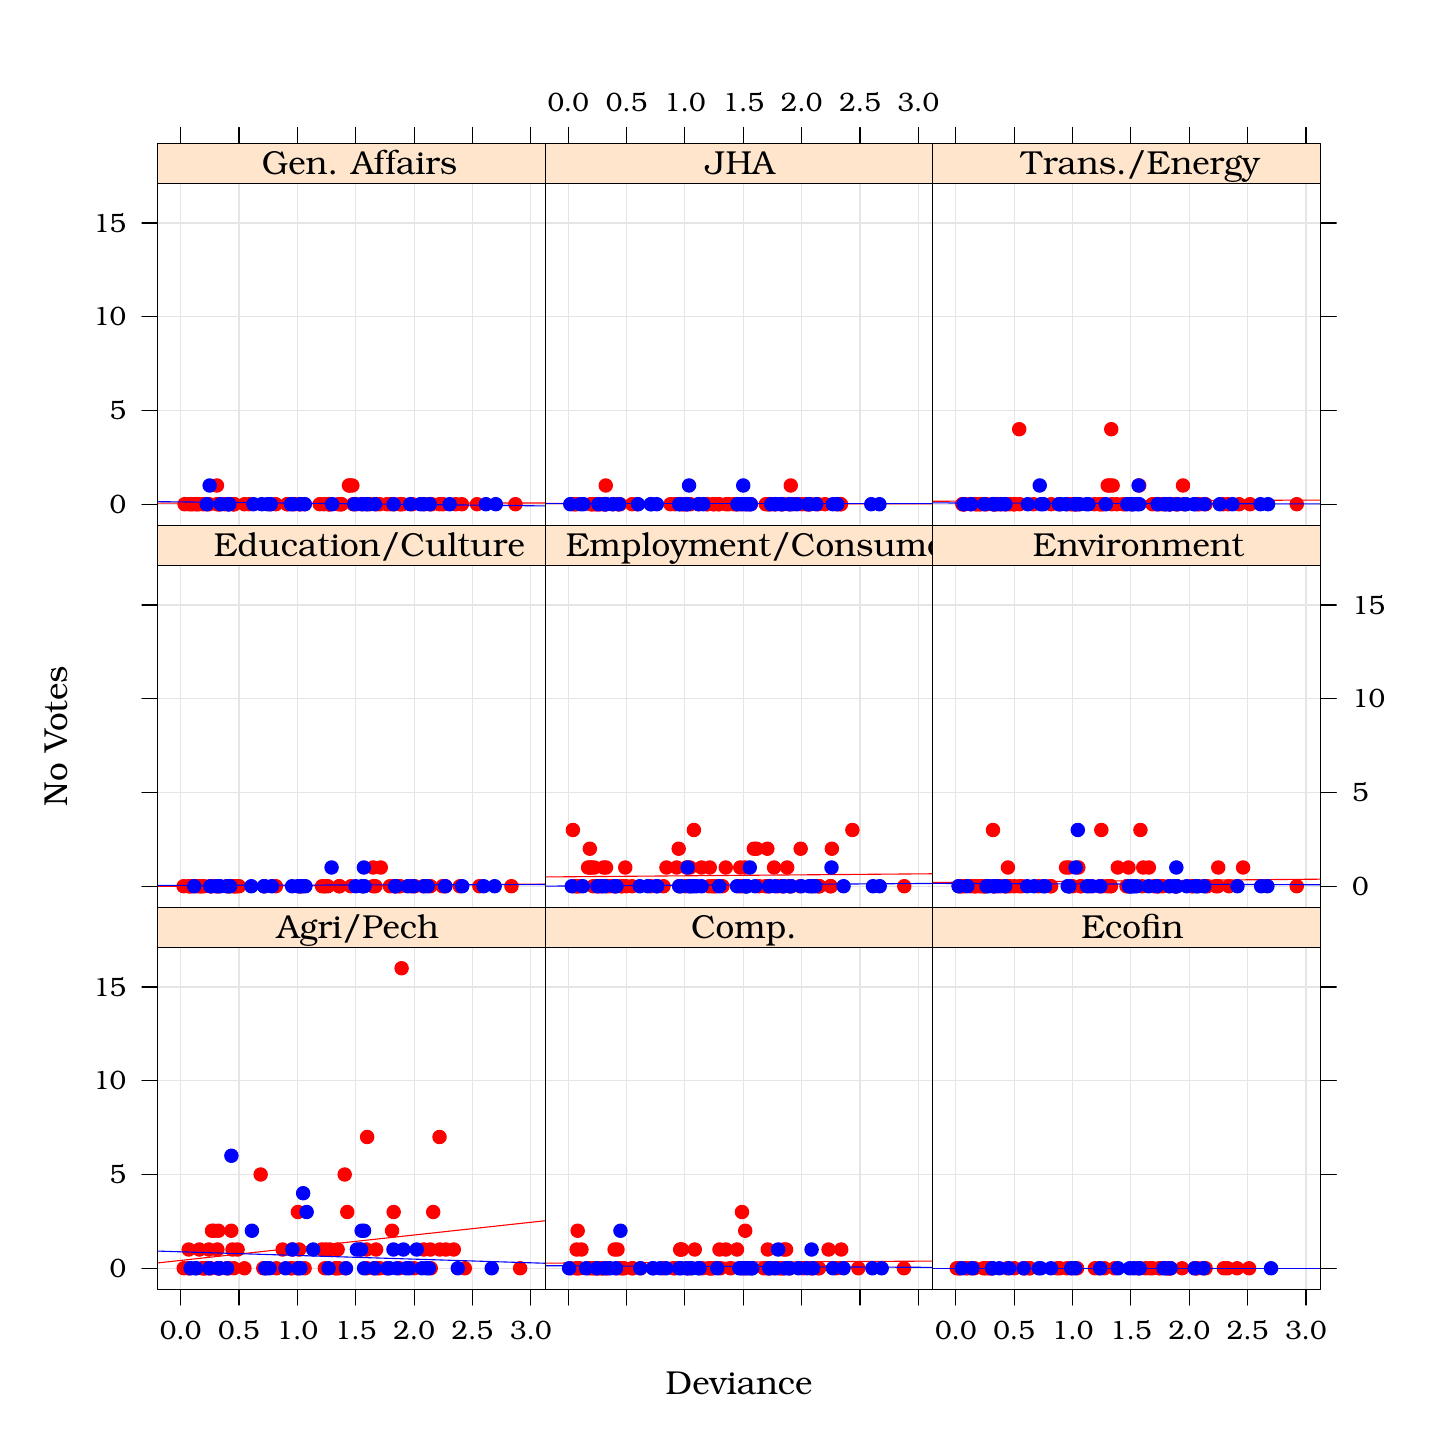
\begin{tikzpicture}[x=1pt,y=1pt]
\definecolor[named]{drawColor}{rgb}{0.00,0.00,0.00}
\definecolor[named]{fillColor}{rgb}{1.00,1.00,1.00}
\fill[color=fillColor,] (0,0) rectangle (505.89,505.89);
\begin{scope}
\path[clip] (  0.00,  0.00) rectangle (505.89,505.89);
\end{scope}
\begin{scope}
\path[clip] (  0.00,  0.00) rectangle (505.89,505.89);

\draw[fill opacity=0.00,draw opacity=0.00,] (  0.00,  0.00) rectangle (505.89,505.89);
\definecolor[named]{drawColor}{rgb}{0.00,0.00,0.00}

\node[color=drawColor,anchor=base,inner sep=0pt, outer sep=0pt, scale=  1.20] at (257.08, 12.04) {Deviance%
};
\end{scope}
\begin{scope}
\path[clip] (  0.00,  0.00) rectangle (505.89,505.89);
\definecolor[named]{drawColor}{rgb}{0.00,0.00,0.00}

\node[rotate= 90.00,color=drawColor,anchor=base,inner sep=0pt, outer sep=0pt, scale=  1.20] at ( 14.29,249.85) {No Votes%
};
\end{scope}
\begin{scope}
\path[clip] (  0.00,  0.00) rectangle (505.89,505.89);
\end{scope}
\begin{scope}
\path[clip] (  0.00,  0.00) rectangle (505.89,505.89);
\end{scope}
\begin{scope}
\path[clip] (  0.00,  0.00) rectangle (505.89,505.89);
\end{scope}
\begin{scope}
\path[clip] ( 46.98, 50.02) rectangle (187.04,173.60);
\end{scope}
\begin{scope}
\path[clip] (  0.00,  0.00) rectangle (505.89,505.89);
\end{scope}
\begin{scope}
\path[clip] (  0.00,  0.00) rectangle (505.89,505.89);
\end{scope}
\begin{scope}
\path[clip] (  0.00,  0.00) rectangle (505.89,505.89);
\end{scope}
\begin{scope}
\path[clip] (  0.00,  0.00) rectangle (505.89,505.89);
\definecolor[named]{drawColor}{rgb}{0.00,0.00,0.00}

\draw[color=drawColor,line cap=round,line join=round,fill opacity=0.00,] ( 46.98, 57.60) -- ( 41.29, 57.60);

\draw[color=drawColor,line cap=round,line join=round,fill opacity=0.00,] ( 46.98, 91.48) -- ( 41.29, 91.48);

\draw[color=drawColor,line cap=round,line join=round,fill opacity=0.00,] ( 46.98,125.36) -- ( 41.29,125.36);

\draw[color=drawColor,line cap=round,line join=round,fill opacity=0.00,] ( 46.98,159.24) -- ( 41.29,159.24);

\node[color=drawColor,anchor=base east,inner sep=0pt, outer sep=0pt, scale=  0.96] at ( 35.60, 54.30) {0%
};

\node[color=drawColor,anchor=base east,inner sep=0pt, outer sep=0pt, scale=  0.96] at ( 35.60, 88.18) {5%
};

\node[color=drawColor,anchor=base east,inner sep=0pt, outer sep=0pt, scale=  0.96] at ( 35.60,122.05) {10%
};

\node[color=drawColor,anchor=base east,inner sep=0pt, outer sep=0pt, scale=  0.96] at ( 35.60,155.93) {15%
};
\end{scope}
\begin{scope}
\path[clip] (  0.00,  0.00) rectangle (505.89,505.89);
\end{scope}
\begin{scope}
\path[clip] (  0.00,  0.00) rectangle (505.89,505.89);
\definecolor[named]{drawColor}{rgb}{0.00,0.00,0.00}

\draw[color=drawColor,line cap=round,line join=round,fill opacity=0.00,] ( 55.26, 50.02) -- ( 55.26, 44.32);

\draw[color=drawColor,line cap=round,line join=round,fill opacity=0.00,] ( 76.35, 50.02) -- ( 76.35, 44.32);

\draw[color=drawColor,line cap=round,line join=round,fill opacity=0.00,] ( 97.44, 50.02) -- ( 97.44, 44.32);

\draw[color=drawColor,line cap=round,line join=round,fill opacity=0.00,] (118.53, 50.02) -- (118.53, 44.32);

\draw[color=drawColor,line cap=round,line join=round,fill opacity=0.00,] (139.62, 50.02) -- (139.62, 44.32);

\draw[color=drawColor,line cap=round,line join=round,fill opacity=0.00,] (160.70, 50.02) -- (160.70, 44.32);

\draw[color=drawColor,line cap=round,line join=round,fill opacity=0.00,] (181.79, 50.02) -- (181.79, 44.32);

\node[color=drawColor,anchor=base,inner sep=0pt, outer sep=0pt, scale=  0.96] at ( 55.26, 32.02) {0.0%
};

\node[color=drawColor,anchor=base,inner sep=0pt, outer sep=0pt, scale=  0.96] at ( 76.35, 32.02) {0.5%
};

\node[color=drawColor,anchor=base,inner sep=0pt, outer sep=0pt, scale=  0.96] at ( 97.44, 32.02) {1.0%
};

\node[color=drawColor,anchor=base,inner sep=0pt, outer sep=0pt, scale=  0.96] at (118.53, 32.02) {1.5%
};

\node[color=drawColor,anchor=base,inner sep=0pt, outer sep=0pt, scale=  0.96] at (139.62, 32.02) {2.0%
};

\node[color=drawColor,anchor=base,inner sep=0pt, outer sep=0pt, scale=  0.96] at (160.70, 32.02) {2.5%
};

\node[color=drawColor,anchor=base,inner sep=0pt, outer sep=0pt, scale=  0.96] at (181.79, 32.02) {3.0%
};
\end{scope}
\begin{scope}
\path[clip] (  0.00,  0.00) rectangle (505.89,505.89);
\end{scope}
\begin{scope}
\path[clip] ( 46.98, 50.02) rectangle (187.04,173.60);
\definecolor[named]{drawColor}{rgb}{0.90,0.90,0.90}

\draw[color=drawColor,line cap=round,line join=round,fill opacity=0.00,] ( 46.98, 57.60) -- (187.04, 57.60);

\draw[color=drawColor,line cap=round,line join=round,fill opacity=0.00,] ( 46.98, 91.48) -- (187.04, 91.48);

\draw[color=drawColor,line cap=round,line join=round,fill opacity=0.00,] ( 46.98,125.36) -- (187.04,125.36);

\draw[color=drawColor,line cap=round,line join=round,fill opacity=0.00,] ( 46.98,159.24) -- (187.04,159.24);

\draw[color=drawColor,line cap=round,line join=round,fill opacity=0.00,] ( 55.26, 50.02) -- ( 55.26,173.60);

\draw[color=drawColor,line cap=round,line join=round,fill opacity=0.00,] ( 76.35, 50.02) -- ( 76.35,173.60);

\draw[color=drawColor,line cap=round,line join=round,fill opacity=0.00,] ( 97.44, 50.02) -- ( 97.44,173.60);

\draw[color=drawColor,line cap=round,line join=round,fill opacity=0.00,] (118.53, 50.02) -- (118.53,173.60);

\draw[color=drawColor,line cap=round,line join=round,fill opacity=0.00,] (139.62, 50.02) -- (139.62,173.60);

\draw[color=drawColor,line cap=round,line join=round,fill opacity=0.00,] (160.70, 50.02) -- (160.70,173.60);

\draw[color=drawColor,line cap=round,line join=round,fill opacity=0.00,] (181.79, 50.02) -- (181.79,173.60);
\definecolor[named]{drawColor}{rgb}{1.00,0.00,0.00}
\definecolor[named]{fillColor}{rgb}{1.00,0.00,0.00}

\draw[color=drawColor,line cap=round,line join=round,fill=fillColor,] ( 72.02, 57.60) circle (  2.41);

\draw[color=drawColor,line cap=round,line join=round,fill=fillColor,] ( 72.67, 57.60) circle (  2.41);

\draw[color=drawColor,line cap=round,line join=round,fill=fillColor,] ( 75.86, 64.38) circle (  2.41);

\draw[color=drawColor,line cap=round,line join=round,fill=fillColor,] (153.97, 64.38) circle (  2.41);

\draw[color=drawColor,line cap=round,line join=round,fill=fillColor,] ( 78.32, 57.60) circle (  2.41);

\draw[color=drawColor,line cap=round,line join=round,fill=fillColor,] (122.60, 57.60) circle (  2.41);

\draw[color=drawColor,line cap=round,line join=round,fill=fillColor,] ( 97.43, 57.60) circle (  2.41);

\draw[color=drawColor,line cap=round,line join=round,fill=fillColor,] ( 58.22, 57.60) circle (  2.41);

\draw[color=drawColor,line cap=round,line join=round,fill=fillColor,] ( 63.46, 57.60) circle (  2.41);

\draw[color=drawColor,line cap=round,line join=round,fill=fillColor,] ( 65.52, 57.60) circle (  2.41);

\draw[color=drawColor,line cap=round,line join=round,fill=fillColor,] ( 84.18, 91.48) circle (  2.41);

\draw[color=drawColor,line cap=round,line join=round,fill=fillColor,] ( 74.01, 64.38) circle (  2.41);

\draw[color=drawColor,line cap=round,line join=round,fill=fillColor,] ( 66.09, 57.60) circle (  2.41);

\draw[color=drawColor,line cap=round,line join=round,fill=fillColor,] ( 69.39, 57.60) circle (  2.41);

\draw[color=drawColor,line cap=round,line join=round,fill=fillColor,] (122.67,105.03) circle (  2.41);

\draw[color=drawColor,line cap=round,line join=round,fill=fillColor,] (132.25, 77.93) circle (  2.41);

\draw[color=drawColor,line cap=round,line join=round,fill=fillColor,] (131.67, 71.16) circle (  2.41);

\draw[color=drawColor,line cap=round,line join=round,fill=fillColor,] ( 65.49, 64.38) circle (  2.41);

\draw[color=drawColor,line cap=round,line join=round,fill=fillColor,] ( 85.14, 57.60) circle (  2.41);

\draw[color=drawColor,line cap=round,line join=round,fill=fillColor,] ( 62.04, 64.38) circle (  2.41);

\draw[color=drawColor,line cap=round,line join=round,fill=fillColor,] ( 95.24, 57.60) circle (  2.41);

\draw[color=drawColor,line cap=round,line join=round,fill=fillColor,] ( 68.59, 57.60) circle (  2.41);

\draw[color=drawColor,line cap=round,line join=round,fill=fillColor,] ( 68.90, 71.16) circle (  2.41);

\draw[color=drawColor,line cap=round,line join=round,fill=fillColor,] (139.66, 57.60) circle (  2.41);

\draw[color=drawColor,line cap=round,line join=round,fill=fillColor,] (143.13, 64.38) circle (  2.41);

\draw[color=drawColor,line cap=round,line join=round,fill=fillColor,] (146.54, 77.93) circle (  2.41);

\draw[color=drawColor,line cap=round,line join=round,fill=fillColor,] (100.06, 57.60) circle (  2.41);

\draw[color=drawColor,line cap=round,line join=round,fill=fillColor,] ( 95.59, 64.38) circle (  2.41);

\draw[color=drawColor,line cap=round,line join=round,fill=fillColor,] (111.56, 57.60) circle (  2.41);

\draw[color=drawColor,line cap=round,line join=round,fill=fillColor,] (114.92, 57.60) circle (  2.41);

\draw[color=drawColor,line cap=round,line join=round,fill=fillColor,] ( 68.55, 64.38) circle (  2.41);

\draw[color=drawColor,line cap=round,line join=round,fill=fillColor,] (119.97, 64.38) circle (  2.41);

\draw[color=drawColor,line cap=round,line join=round,fill=fillColor,] (157.96, 57.60) circle (  2.41);

\draw[color=drawColor,line cap=round,line join=round,fill=fillColor,] ( 97.65, 77.93) circle (  2.41);

\draw[color=drawColor,line cap=round,line join=round,fill=fillColor,] ( 98.11, 64.38) circle (  2.41);

\draw[color=drawColor,line cap=round,line join=round,fill=fillColor,] ( 63.05, 57.60) circle (  2.41);

\draw[color=drawColor,line cap=round,line join=round,fill=fillColor,] ( 95.34, 57.60) circle (  2.41);

\draw[color=drawColor,line cap=round,line join=round,fill=fillColor,] (148.92, 64.38) circle (  2.41);

\draw[color=drawColor,line cap=round,line join=round,fill=fillColor,] (115.49, 77.93) circle (  2.41);

\draw[color=drawColor,line cap=round,line join=round,fill=fillColor,] ( 58.24, 57.60) circle (  2.41);

\draw[color=drawColor,line cap=round,line join=round,fill=fillColor,] ( 56.40, 57.60) circle (  2.41);

\draw[color=drawColor,line cap=round,line join=round,fill=fillColor,] (145.51, 64.38) circle (  2.41);

\draw[color=drawColor,line cap=round,line join=round,fill=fillColor,] (122.46, 64.38) circle (  2.41);

\draw[color=drawColor,line cap=round,line join=round,fill=fillColor,] (125.89, 64.38) circle (  2.41);

\draw[color=drawColor,line cap=round,line join=round,fill=fillColor,] (134.26, 57.60) circle (  2.41);

\draw[color=drawColor,line cap=round,line join=round,fill=fillColor,] (135.11,166.01) circle (  2.41);

\draw[color=drawColor,line cap=round,line join=round,fill=fillColor,] (151.13, 64.38) circle (  2.41);

\draw[color=drawColor,line cap=round,line join=round,fill=fillColor,] ( 89.88, 57.60) circle (  2.41);

\draw[color=drawColor,line cap=round,line join=round,fill=fillColor,] (129.79, 57.60) circle (  2.41);

\draw[color=drawColor,line cap=round,line join=round,fill=fillColor,] ( 58.18, 64.38) circle (  2.41);

\draw[color=drawColor,line cap=round,line join=round,fill=fillColor,] (111.22, 57.60) circle (  2.41);

\draw[color=drawColor,line cap=round,line join=round,fill=fillColor,] ( 66.60, 71.16) circle (  2.41);

\draw[color=drawColor,line cap=round,line join=round,fill=fillColor,] ( 63.95, 57.60) circle (  2.41);

\draw[color=drawColor,line cap=round,line join=round,fill=fillColor,] ( 63.91, 57.60) circle (  2.41);

\draw[color=drawColor,line cap=round,line join=round,fill=fillColor,] ( 67.19, 71.16) circle (  2.41);

\draw[color=drawColor,line cap=round,line join=round,fill=fillColor,] (109.14, 64.38) circle (  2.41);

\draw[color=drawColor,line cap=round,line join=round,fill=fillColor,] ( 74.47, 57.60) circle (  2.41);

\draw[color=drawColor,line cap=round,line join=round,fill=fillColor,] ( 92.13, 64.38) circle (  2.41);

\draw[color=drawColor,line cap=round,line join=round,fill=fillColor,] (125.23, 57.60) circle (  2.41);

\draw[color=drawColor,line cap=round,line join=round,fill=fillColor,] (112.01, 64.38) circle (  2.41);

\draw[color=drawColor,line cap=round,line join=round,fill=fillColor,] (177.95, 57.60) circle (  2.41);

\draw[color=drawColor,line cap=round,line join=round,fill=fillColor,] (145.65, 57.60) circle (  2.41);

\draw[color=drawColor,line cap=round,line join=round,fill=fillColor,] (126.39, 57.60) circle (  2.41);

\draw[color=drawColor,line cap=round,line join=round,fill=fillColor,] (127.24, 57.60) circle (  2.41);

\draw[color=drawColor,line cap=round,line join=round,fill=fillColor,] (114.55, 91.48) circle (  2.41);

\draw[color=drawColor,line cap=round,line join=round,fill=fillColor,] (148.82,105.03) circle (  2.41);

\draw[color=drawColor,line cap=round,line join=round,fill=fillColor,] (107.75, 64.38) circle (  2.41);

\draw[color=drawColor,line cap=round,line join=round,fill=fillColor,] ( 73.58, 71.16) circle (  2.41);

\draw[color=drawColor,line cap=round,line join=round,fill=fillColor,] (112.48, 57.60) circle (  2.41);

\draw[color=drawColor,line cap=round,line join=round,fill=fillColor,] (106.31, 64.38) circle (  2.41);

\draw[color=drawColor,line cap=round,line join=round,fill=fillColor,] (107.39, 57.60) circle (  2.41);

\draw[color=drawColor,line cap=round,line join=round,fill opacity=0.00,] (187.04, 74.78) --
	( 46.98, 59.53);
\definecolor[named]{drawColor}{rgb}{0.00,0.00,1.00}
\definecolor[named]{fillColor}{rgb}{0.00,0.00,1.00}

\draw[color=drawColor,line cap=round,line join=round,fill=fillColor,] ( 95.67, 64.38) circle (  2.41);

\draw[color=drawColor,line cap=round,line join=round,fill=fillColor,] (142.48, 57.60) circle (  2.41);

\draw[color=drawColor,line cap=round,line join=round,fill=fillColor,] (121.55, 71.16) circle (  2.41);

\draw[color=drawColor,line cap=round,line join=round,fill=fillColor,] ( 60.78, 57.60) circle (  2.41);

\draw[color=drawColor,line cap=round,line join=round,fill=fillColor,] ( 58.87, 57.60) circle (  2.41);

\draw[color=drawColor,line cap=round,line join=round,fill=fillColor,] ( 60.78, 57.60) circle (  2.41);

\draw[color=drawColor,line cap=round,line join=round,fill=fillColor,] (130.07, 57.60) circle (  2.41);

\draw[color=drawColor,line cap=round,line join=round,fill=fillColor,] ( 81.03, 71.16) circle (  2.41);

\draw[color=drawColor,line cap=round,line join=round,fill=fillColor,] ( 69.34, 57.60) circle (  2.41);

\draw[color=drawColor,line cap=round,line join=round,fill=fillColor,] ( 99.54, 84.71) circle (  2.41);

\draw[color=drawColor,line cap=round,line join=round,fill=fillColor,] (103.17, 64.38) circle (  2.41);

\draw[color=drawColor,line cap=round,line join=round,fill=fillColor,] (140.57, 64.38) circle (  2.41);

\draw[color=drawColor,line cap=round,line join=round,fill=fillColor,] (167.68, 57.60) circle (  2.41);

\draw[color=drawColor,line cap=round,line join=round,fill=fillColor,] (136.87, 57.60) circle (  2.41);

\draw[color=drawColor,line cap=round,line join=round,fill=fillColor,] (137.96, 57.60) circle (  2.41);

\draw[color=drawColor,line cap=round,line join=round,fill=fillColor,] ( 93.20, 57.60) circle (  2.41);

\draw[color=drawColor,line cap=round,line join=round,fill=fillColor,] (120.69, 71.16) circle (  2.41);

\draw[color=drawColor,line cap=round,line join=round,fill=fillColor,] (100.81, 77.93) circle (  2.41);

\draw[color=drawColor,line cap=round,line join=round,fill=fillColor,] ( 97.86, 57.60) circle (  2.41);

\draw[color=drawColor,line cap=round,line join=round,fill=fillColor,] (118.97, 64.38) circle (  2.41);

\draw[color=drawColor,line cap=round,line join=round,fill=fillColor,] (121.56, 57.60) circle (  2.41);

\draw[color=drawColor,line cap=round,line join=round,fill=fillColor,] (120.43, 64.38) circle (  2.41);

\draw[color=drawColor,line cap=round,line join=round,fill=fillColor,] (125.32, 57.60) circle (  2.41);

\draw[color=drawColor,line cap=round,line join=round,fill=fillColor,] ( 69.13, 57.60) circle (  2.41);

\draw[color=drawColor,line cap=round,line join=round,fill=fillColor,] (144.09, 57.60) circle (  2.41);

\draw[color=drawColor,line cap=round,line join=round,fill=fillColor,] ( 85.87, 57.60) circle (  2.41);

\draw[color=drawColor,line cap=round,line join=round,fill=fillColor,] ( 87.38, 57.60) circle (  2.41);

\draw[color=drawColor,line cap=round,line join=round,fill=fillColor,] (135.77, 64.38) circle (  2.41);

\draw[color=drawColor,line cap=round,line join=round,fill=fillColor,] (132.18, 64.38) circle (  2.41);

\draw[color=drawColor,line cap=round,line join=round,fill=fillColor,] (155.42, 57.60) circle (  2.41);

\draw[color=drawColor,line cap=round,line join=round,fill=fillColor,] (144.99, 57.60) circle (  2.41);

\draw[color=drawColor,line cap=round,line join=round,fill=fillColor,] ( 65.62, 57.60) circle (  2.41);

\draw[color=drawColor,line cap=round,line join=round,fill=fillColor,] ( 98.56, 57.60) circle (  2.41);

\draw[color=drawColor,line cap=round,line join=round,fill=fillColor,] ( 68.94, 57.60) circle (  2.41);

\draw[color=drawColor,line cap=round,line join=round,fill=fillColor,] ( 72.03, 57.60) circle (  2.41);

\draw[color=drawColor,line cap=round,line join=round,fill=fillColor,] (115.01, 57.60) circle (  2.41);

\draw[color=drawColor,line cap=round,line join=round,fill=fillColor,] (108.74, 57.60) circle (  2.41);

\draw[color=drawColor,line cap=round,line join=round,fill=fillColor,] ( 73.61, 98.26) circle (  2.41);

\draw[color=drawColor,line cap=round,line join=round,fill=fillColor,] ( 86.05, 57.60) circle (  2.41);

\draw[color=drawColor,line cap=round,line join=round,fill=fillColor,] (133.40, 57.60) circle (  2.41);

\draw[color=drawColor,line cap=round,line join=round,fill=fillColor,] (130.77, 57.60) circle (  2.41);

\draw[color=drawColor,line cap=round,line join=round,fill opacity=0.00,] (187.04, 59.41) --
	( 46.98, 63.81);
\end{scope}
\begin{scope}
\path[clip] (  0.00,  0.00) rectangle (505.89,505.89);
\end{scope}
\begin{scope}
\path[clip] (  0.00,  0.00) rectangle (505.89,505.89);
\definecolor[named]{drawColor}{rgb}{0.00,0.00,0.00}

\draw[color=drawColor,line cap=round,line join=round,fill opacity=0.00,] ( 46.98, 50.02) rectangle (187.04,173.60);
\end{scope}
\begin{scope}
\path[clip] (  0.00,  0.00) rectangle (505.89,505.89);
\end{scope}
\begin{scope}
\path[clip] (  0.00,  0.00) rectangle (505.89,505.89);
\end{scope}
\begin{scope}
\path[clip] ( 46.98,173.60) rectangle (187.04,188.06);
\definecolor[named]{drawColor}{rgb}{1.00,0.90,0.80}
\definecolor[named]{fillColor}{rgb}{1.00,0.90,0.80}

\draw[color=drawColor,line cap=round,line join=round,fill=fillColor,] ( 46.98,173.60) rectangle (187.04,188.06);
\definecolor[named]{drawColor}{rgb}{0.00,0.00,0.00}

\node[color=drawColor,anchor=base west,inner sep=0pt, outer sep=0pt, scale=  1.20] at ( 90.09,176.70) {Agri/Pech%
};
\end{scope}
\begin{scope}
\path[clip] (  0.00,  0.00) rectangle (505.89,505.89);
\end{scope}
\begin{scope}
\path[clip] (  0.00,  0.00) rectangle (505.89,505.89);
\definecolor[named]{drawColor}{rgb}{0.00,0.00,0.00}

\draw[color=drawColor,line cap=round,line join=round,fill opacity=0.00,] ( 46.98,173.60) rectangle (187.04,188.06);
\end{scope}
\begin{scope}
\path[clip] (  0.00,  0.00) rectangle (505.89,505.89);
\end{scope}
\begin{scope}
\path[clip] (  0.00,  0.00) rectangle (505.89,505.89);
\end{scope}
\begin{scope}
\path[clip] (187.04, 50.02) rectangle (327.11,173.60);
\end{scope}
\begin{scope}
\path[clip] (  0.00,  0.00) rectangle (505.89,505.89);
\end{scope}
\begin{scope}
\path[clip] (  0.00,  0.00) rectangle (505.89,505.89);
\end{scope}
\begin{scope}
\path[clip] (  0.00,  0.00) rectangle (505.89,505.89);
\end{scope}
\begin{scope}
\path[clip] (  0.00,  0.00) rectangle (505.89,505.89);
\end{scope}
\begin{scope}
\path[clip] (  0.00,  0.00) rectangle (505.89,505.89);
\end{scope}
\begin{scope}
\path[clip] (  0.00,  0.00) rectangle (505.89,505.89);
\definecolor[named]{drawColor}{rgb}{0.00,0.00,0.00}

\draw[color=drawColor,line cap=round,line join=round,fill opacity=0.00,] (195.33, 50.02) -- (195.33, 44.32);

\draw[color=drawColor,line cap=round,line join=round,fill opacity=0.00,] (216.42, 50.02) -- (216.42, 44.32);

\draw[color=drawColor,line cap=round,line join=round,fill opacity=0.00,] (237.50, 50.02) -- (237.50, 44.32);

\draw[color=drawColor,line cap=round,line join=round,fill opacity=0.00,] (258.59, 50.02) -- (258.59, 44.32);

\draw[color=drawColor,line cap=round,line join=round,fill opacity=0.00,] (279.68, 50.02) -- (279.68, 44.32);

\draw[color=drawColor,line cap=round,line join=round,fill opacity=0.00,] (300.77, 50.02) -- (300.77, 44.32);

\draw[color=drawColor,line cap=round,line join=round,fill opacity=0.00,] (321.86, 50.02) -- (321.86, 44.32);
\end{scope}
\begin{scope}
\path[clip] (  0.00,  0.00) rectangle (505.89,505.89);
\end{scope}
\begin{scope}
\path[clip] (187.04, 50.02) rectangle (327.11,173.60);
\definecolor[named]{drawColor}{rgb}{0.90,0.90,0.90}

\draw[color=drawColor,line cap=round,line join=round,fill opacity=0.00,] (187.04, 57.60) -- (327.11, 57.60);

\draw[color=drawColor,line cap=round,line join=round,fill opacity=0.00,] (187.04, 91.48) -- (327.11, 91.48);

\draw[color=drawColor,line cap=round,line join=round,fill opacity=0.00,] (187.04,125.36) -- (327.11,125.36);

\draw[color=drawColor,line cap=round,line join=round,fill opacity=0.00,] (187.04,159.24) -- (327.11,159.24);

\draw[color=drawColor,line cap=round,line join=round,fill opacity=0.00,] (195.33, 50.02) -- (195.33,173.60);

\draw[color=drawColor,line cap=round,line join=round,fill opacity=0.00,] (216.42, 50.02) -- (216.42,173.60);

\draw[color=drawColor,line cap=round,line join=round,fill opacity=0.00,] (237.50, 50.02) -- (237.50,173.60);

\draw[color=drawColor,line cap=round,line join=round,fill opacity=0.00,] (258.59, 50.02) -- (258.59,173.60);

\draw[color=drawColor,line cap=round,line join=round,fill opacity=0.00,] (279.68, 50.02) -- (279.68,173.60);

\draw[color=drawColor,line cap=round,line join=round,fill opacity=0.00,] (300.77, 50.02) -- (300.77,173.60);

\draw[color=drawColor,line cap=round,line join=round,fill opacity=0.00,] (321.86, 50.02) -- (321.86,173.60);
\definecolor[named]{drawColor}{rgb}{1.00,0.00,0.00}
\definecolor[named]{fillColor}{rgb}{1.00,0.00,0.00}

\draw[color=drawColor,line cap=round,line join=round,fill=fillColor,] (212.83, 57.60) circle (  2.41);

\draw[color=drawColor,line cap=round,line join=round,fill=fillColor,] (212.09, 64.38) circle (  2.41);

\draw[color=drawColor,line cap=round,line join=round,fill=fillColor,] (215.50, 57.60) circle (  2.41);

\draw[color=drawColor,line cap=round,line join=round,fill=fillColor,] (280.10, 57.60) circle (  2.41);

\draw[color=drawColor,line cap=round,line join=round,fill=fillColor,] (218.39, 57.60) circle (  2.41);

\draw[color=drawColor,line cap=round,line join=round,fill=fillColor,] (259.69, 57.60) circle (  2.41);

\draw[color=drawColor,line cap=round,line join=round,fill=fillColor,] (236.45, 64.38) circle (  2.41);

\draw[color=drawColor,line cap=round,line join=round,fill=fillColor,] (198.29, 57.60) circle (  2.41);

\draw[color=drawColor,line cap=round,line join=round,fill=fillColor,] (202.68, 57.60) circle (  2.41);

\draw[color=drawColor,line cap=round,line join=round,fill=fillColor,] (206.03, 57.60) circle (  2.41);

\draw[color=drawColor,line cap=round,line join=round,fill=fillColor,] (241.05, 64.38) circle (  2.41);

\draw[color=drawColor,line cap=round,line join=round,fill=fillColor,] (218.62, 57.60) circle (  2.41);

\draw[color=drawColor,line cap=round,line join=round,fill=fillColor,] (207.62, 57.60) circle (  2.41);

\draw[color=drawColor,line cap=round,line join=round,fill=fillColor,] (209.42, 57.60) circle (  2.41);

\draw[color=drawColor,line cap=round,line join=round,fill=fillColor,] (258.11, 77.93) circle (  2.41);

\draw[color=drawColor,line cap=round,line join=round,fill=fillColor,] (272.03, 57.60) circle (  2.41);

\draw[color=drawColor,line cap=round,line join=round,fill=fillColor,] (271.54, 57.60) circle (  2.41);

\draw[color=drawColor,line cap=round,line join=round,fill=fillColor,] (272.79, 57.60) circle (  2.41);

\draw[color=drawColor,line cap=round,line join=round,fill=fillColor,] (205.84, 57.60) circle (  2.41);

\draw[color=drawColor,line cap=round,line join=round,fill=fillColor,] (221.50, 57.60) circle (  2.41);

\draw[color=drawColor,line cap=round,line join=round,fill=fillColor,] (199.44, 57.60) circle (  2.41);

\draw[color=drawColor,line cap=round,line join=round,fill=fillColor,] (207.41, 57.60) circle (  2.41);

\draw[color=drawColor,line cap=round,line join=round,fill=fillColor,] (235.95, 64.38) circle (  2.41);

\draw[color=drawColor,line cap=round,line join=round,fill=fillColor,] (213.13, 64.38) circle (  2.41);

\draw[color=drawColor,line cap=round,line join=round,fill=fillColor,] (209.37, 57.60) circle (  2.41);

\draw[color=drawColor,line cap=round,line join=round,fill=fillColor,] (283.25, 57.60) circle (  2.41);

\draw[color=drawColor,line cap=round,line join=round,fill=fillColor,] (289.40, 64.38) circle (  2.41);

\draw[color=drawColor,line cap=round,line join=round,fill=fillColor,] (239.49, 57.60) circle (  2.41);

\draw[color=drawColor,line cap=round,line join=round,fill=fillColor,] (235.78, 64.38) circle (  2.41);

\draw[color=drawColor,line cap=round,line join=round,fill=fillColor,] (243.80, 57.60) circle (  2.41);

\draw[color=drawColor,line cap=round,line join=round,fill=fillColor,] (253.98, 57.60) circle (  2.41);

\draw[color=drawColor,line cap=round,line join=round,fill=fillColor,] (207.66, 57.60) circle (  2.41);

\draw[color=drawColor,line cap=round,line join=round,fill=fillColor,] (272.86, 57.60) circle (  2.41);

\draw[color=drawColor,line cap=round,line join=round,fill=fillColor,] (300.16, 57.60) circle (  2.41);

\draw[color=drawColor,line cap=round,line join=round,fill=fillColor,] (233.37, 57.60) circle (  2.41);

\draw[color=drawColor,line cap=round,line join=round,fill=fillColor,] (238.16, 57.60) circle (  2.41);

\draw[color=drawColor,line cap=round,line join=round,fill=fillColor,] (204.49, 57.60) circle (  2.41);

\draw[color=drawColor,line cap=round,line join=round,fill=fillColor,] (246.38, 57.60) circle (  2.41);

\draw[color=drawColor,line cap=round,line join=round,fill=fillColor,] (285.96, 57.60) circle (  2.41);

\draw[color=drawColor,line cap=round,line join=round,fill=fillColor,] (250.28, 57.60) circle (  2.41);

\draw[color=drawColor,line cap=round,line join=round,fill=fillColor,] (198.67, 57.60) circle (  2.41);

\draw[color=drawColor,line cap=round,line join=round,fill=fillColor,] (196.18, 57.60) circle (  2.41);

\draw[color=drawColor,line cap=round,line join=round,fill=fillColor,] (285.58, 57.60) circle (  2.41);

\draw[color=drawColor,line cap=round,line join=round,fill=fillColor,] (256.31, 64.38) circle (  2.41);

\draw[color=drawColor,line cap=round,line join=round,fill=fillColor,] (269.72, 57.60) circle (  2.41);

\draw[color=drawColor,line cap=round,line join=round,fill=fillColor,] (274.04, 64.38) circle (  2.41);

\draw[color=drawColor,line cap=round,line join=round,fill=fillColor,] (275.41, 57.60) circle (  2.41);

\draw[color=drawColor,line cap=round,line join=round,fill=fillColor,] (283.41, 57.60) circle (  2.41);

\draw[color=drawColor,line cap=round,line join=round,fill=fillColor,] (292.20, 57.60) circle (  2.41);

\draw[color=drawColor,line cap=round,line join=round,fill=fillColor,] (229.75, 57.60) circle (  2.41);

\draw[color=drawColor,line cap=round,line join=round,fill=fillColor,] (258.65, 57.60) circle (  2.41);

\draw[color=drawColor,line cap=round,line join=round,fill=fillColor,] (198.38, 64.38) circle (  2.41);

\draw[color=drawColor,line cap=round,line join=round,fill=fillColor,] (249.98, 64.38) circle (  2.41);

\draw[color=drawColor,line cap=round,line join=round,fill=fillColor,] (200.11, 64.38) circle (  2.41);

\draw[color=drawColor,line cap=round,line join=round,fill=fillColor,] (205.13, 57.60) circle (  2.41);

\draw[color=drawColor,line cap=round,line join=round,fill=fillColor,] (203.64, 57.60) circle (  2.41);

\draw[color=drawColor,line cap=round,line join=round,fill=fillColor,] (198.74, 71.16) circle (  2.41);

\draw[color=drawColor,line cap=round,line join=round,fill=fillColor,] (246.60, 57.60) circle (  2.41);

\draw[color=drawColor,line cap=round,line join=round,fill=fillColor,] (215.01, 57.60) circle (  2.41);

\draw[color=drawColor,line cap=round,line join=round,fill=fillColor,] (233.77, 57.60) circle (  2.41);

\draw[color=drawColor,line cap=round,line join=round,fill=fillColor,] (266.05, 57.60) circle (  2.41);

\draw[color=drawColor,line cap=round,line join=round,fill=fillColor,] (252.31, 64.38) circle (  2.41);

\draw[color=drawColor,line cap=round,line join=round,fill=fillColor,] (316.64, 57.60) circle (  2.41);

\draw[color=drawColor,line cap=round,line join=round,fill=fillColor,] (273.24, 64.38) circle (  2.41);

\draw[color=drawColor,line cap=round,line join=round,fill=fillColor,] (267.27, 57.60) circle (  2.41);

\draw[color=drawColor,line cap=round,line join=round,fill=fillColor,] (267.88, 57.60) circle (  2.41);

\draw[color=drawColor,line cap=round,line join=round,fill=fillColor,] (267.43, 64.38) circle (  2.41);

\draw[color=drawColor,line cap=round,line join=round,fill=fillColor,] (293.97, 64.38) circle (  2.41);

\draw[color=drawColor,line cap=round,line join=round,fill=fillColor,] (247.47, 57.60) circle (  2.41);

\draw[color=drawColor,line cap=round,line join=round,fill=fillColor,] (214.33, 57.60) circle (  2.41);

\draw[color=drawColor,line cap=round,line join=round,fill=fillColor,] (259.28, 71.16) circle (  2.41);

\draw[color=drawColor,line cap=round,line join=round,fill=fillColor,] (246.50, 57.60) circle (  2.41);

\draw[color=drawColor,line cap=round,line join=round,fill=fillColor,] (247.36, 57.60) circle (  2.41);

\draw[color=drawColor,line cap=round,line join=round,fill opacity=0.00,] (327.11, 60.19) --
	(187.04, 59.45);
\definecolor[named]{drawColor}{rgb}{0.00,0.00,1.00}
\definecolor[named]{fillColor}{rgb}{0.00,0.00,1.00}

\draw[color=drawColor,line cap=round,line join=round,fill=fillColor,] (235.40, 57.60) circle (  2.41);

\draw[color=drawColor,line cap=round,line join=round,fill=fillColor,] (283.26, 64.38) circle (  2.41);

\draw[color=drawColor,line cap=round,line join=round,fill=fillColor,] (261.72, 57.60) circle (  2.41);

\draw[color=drawColor,line cap=round,line join=round,fill=fillColor,] (238.48, 57.60) circle (  2.41);

\draw[color=drawColor,line cap=round,line join=round,fill=fillColor,] (201.77, 57.60) circle (  2.41);

\draw[color=drawColor,line cap=round,line join=round,fill=fillColor,] (195.65, 57.60) circle (  2.41);

\draw[color=drawColor,line cap=round,line join=round,fill=fillColor,] (270.30, 57.60) circle (  2.41);

\draw[color=drawColor,line cap=round,line join=round,fill=fillColor,] (221.37, 57.60) circle (  2.41);

\draw[color=drawColor,line cap=round,line join=round,fill=fillColor,] (210.44, 57.60) circle (  2.41);

\draw[color=drawColor,line cap=round,line join=round,fill=fillColor,] (239.94, 57.60) circle (  2.41);

\draw[color=drawColor,line cap=round,line join=round,fill=fillColor,] (290.96, 57.60) circle (  2.41);

\draw[color=drawColor,line cap=round,line join=round,fill=fillColor,] (242.31, 57.60) circle (  2.41);

\draw[color=drawColor,line cap=round,line join=round,fill=fillColor,] (305.25, 57.60) circle (  2.41);

\draw[color=drawColor,line cap=round,line join=round,fill=fillColor,] (281.64, 57.60) circle (  2.41);

\draw[color=drawColor,line cap=round,line join=round,fill=fillColor,] (308.59, 57.60) circle (  2.41);

\draw[color=drawColor,line cap=round,line join=round,fill=fillColor,] (275.12, 57.60) circle (  2.41);

\draw[color=drawColor,line cap=round,line join=round,fill=fillColor,] (261.15, 57.60) circle (  2.41);

\draw[color=drawColor,line cap=round,line join=round,fill=fillColor,] (236.15, 57.60) circle (  2.41);

\draw[color=drawColor,line cap=round,line join=round,fill=fillColor,] (260.17, 57.60) circle (  2.41);

\draw[color=drawColor,line cap=round,line join=round,fill=fillColor,] (242.75, 57.60) circle (  2.41);

\draw[color=drawColor,line cap=round,line join=round,fill=fillColor,] (230.70, 57.60) circle (  2.41);

\draw[color=drawColor,line cap=round,line join=round,fill=fillColor,] (258.88, 57.60) circle (  2.41);

\draw[color=drawColor,line cap=round,line join=round,fill=fillColor,] (261.80, 57.60) circle (  2.41);

\draw[color=drawColor,line cap=round,line join=round,fill=fillColor,] (257.84, 57.60) circle (  2.41);

\draw[color=drawColor,line cap=round,line join=round,fill=fillColor,] (268.25, 57.60) circle (  2.41);

\draw[color=drawColor,line cap=round,line join=round,fill=fillColor,] (208.66, 57.60) circle (  2.41);

\draw[color=drawColor,line cap=round,line join=round,fill=fillColor,] (283.79, 57.60) circle (  2.41);

\draw[color=drawColor,line cap=round,line join=round,fill=fillColor,] (226.01, 57.60) circle (  2.41);

\draw[color=drawColor,line cap=round,line join=round,fill=fillColor,] (228.49, 57.60) circle (  2.41);

\draw[color=drawColor,line cap=round,line join=round,fill=fillColor,] (275.21, 57.60) circle (  2.41);

\draw[color=drawColor,line cap=round,line join=round,fill=fillColor,] (271.18, 64.38) circle (  2.41);

\draw[color=drawColor,line cap=round,line join=round,fill=fillColor,] (294.81, 57.60) circle (  2.41);

\draw[color=drawColor,line cap=round,line join=round,fill=fillColor,] (278.53, 57.60) circle (  2.41);

\draw[color=drawColor,line cap=round,line join=round,fill=fillColor,] (205.77, 57.60) circle (  2.41);

\draw[color=drawColor,line cap=round,line join=round,fill=fillColor,] (238.19, 57.60) circle (  2.41);

\draw[color=drawColor,line cap=round,line join=round,fill=fillColor,] (212.57, 57.60) circle (  2.41);

\draw[color=drawColor,line cap=round,line join=round,fill=fillColor,] (257.15, 57.60) circle (  2.41);

\draw[color=drawColor,line cap=round,line join=round,fill=fillColor,] (249.17, 57.60) circle (  2.41);

\draw[color=drawColor,line cap=round,line join=round,fill=fillColor,] (214.20, 71.16) circle (  2.41);

\draw[color=drawColor,line cap=round,line join=round,fill=fillColor,] (225.92, 57.60) circle (  2.41);

\draw[color=drawColor,line cap=round,line join=round,fill=fillColor,] (273.83, 57.60) circle (  2.41);

\draw[color=drawColor,line cap=round,line join=round,fill=fillColor,] (267.95, 57.60) circle (  2.41);

\draw[color=drawColor,line cap=round,line join=round,fill opacity=0.00,] (327.11, 57.93) --
	(187.04, 58.52);
\end{scope}
\begin{scope}
\path[clip] (  0.00,  0.00) rectangle (505.89,505.89);
\end{scope}
\begin{scope}
\path[clip] (  0.00,  0.00) rectangle (505.89,505.89);
\definecolor[named]{drawColor}{rgb}{0.00,0.00,0.00}

\draw[color=drawColor,line cap=round,line join=round,fill opacity=0.00,] (187.04, 50.02) rectangle (327.11,173.60);
\end{scope}
\begin{scope}
\path[clip] (  0.00,  0.00) rectangle (505.89,505.89);
\end{scope}
\begin{scope}
\path[clip] (  0.00,  0.00) rectangle (505.89,505.89);
\end{scope}
\begin{scope}
\path[clip] (187.04,173.60) rectangle (327.11,188.06);
\definecolor[named]{drawColor}{rgb}{1.00,0.90,0.80}
\definecolor[named]{fillColor}{rgb}{1.00,0.90,0.80}

\draw[color=drawColor,line cap=round,line join=round,fill=fillColor,] (187.04,173.60) rectangle (327.11,188.06);
\definecolor[named]{drawColor}{rgb}{0.00,0.00,0.00}

\node[color=drawColor,anchor=base west,inner sep=0pt, outer sep=0pt, scale=  1.20] at (239.75,176.70) {Comp.%
};
\end{scope}
\begin{scope}
\path[clip] (  0.00,  0.00) rectangle (505.89,505.89);
\end{scope}
\begin{scope}
\path[clip] (  0.00,  0.00) rectangle (505.89,505.89);
\definecolor[named]{drawColor}{rgb}{0.00,0.00,0.00}

\draw[color=drawColor,line cap=round,line join=round,fill opacity=0.00,] (187.04,173.60) rectangle (327.11,188.06);
\end{scope}
\begin{scope}
\path[clip] (  0.00,  0.00) rectangle (505.89,505.89);
\end{scope}
\begin{scope}
\path[clip] (  0.00,  0.00) rectangle (505.89,505.89);
\end{scope}
\begin{scope}
\path[clip] (327.11, 50.02) rectangle (467.18,173.60);
\end{scope}
\begin{scope}
\path[clip] (  0.00,  0.00) rectangle (505.89,505.89);
\end{scope}
\begin{scope}
\path[clip] (  0.00,  0.00) rectangle (505.89,505.89);
\end{scope}
\begin{scope}
\path[clip] (  0.00,  0.00) rectangle (505.89,505.89);
\end{scope}
\begin{scope}
\path[clip] (  0.00,  0.00) rectangle (505.89,505.89);
\end{scope}
\begin{scope}
\path[clip] (  0.00,  0.00) rectangle (505.89,505.89);
\end{scope}
\begin{scope}
\path[clip] (  0.00,  0.00) rectangle (505.89,505.89);
\definecolor[named]{drawColor}{rgb}{0.00,0.00,0.00}

\draw[color=drawColor,line cap=round,line join=round,fill opacity=0.00,] (335.39, 50.02) -- (335.39, 44.32);

\draw[color=drawColor,line cap=round,line join=round,fill opacity=0.00,] (356.48, 50.02) -- (356.48, 44.32);

\draw[color=drawColor,line cap=round,line join=round,fill opacity=0.00,] (377.57, 50.02) -- (377.57, 44.32);

\draw[color=drawColor,line cap=round,line join=round,fill opacity=0.00,] (398.66, 50.02) -- (398.66, 44.32);

\draw[color=drawColor,line cap=round,line join=round,fill opacity=0.00,] (419.75, 50.02) -- (419.75, 44.32);

\draw[color=drawColor,line cap=round,line join=round,fill opacity=0.00,] (440.83, 50.02) -- (440.83, 44.32);

\draw[color=drawColor,line cap=round,line join=round,fill opacity=0.00,] (461.92, 50.02) -- (461.92, 44.32);

\node[color=drawColor,anchor=base,inner sep=0pt, outer sep=0pt, scale=  0.96] at (335.39, 32.02) {0.0%
};

\node[color=drawColor,anchor=base,inner sep=0pt, outer sep=0pt, scale=  0.96] at (356.48, 32.02) {0.5%
};

\node[color=drawColor,anchor=base,inner sep=0pt, outer sep=0pt, scale=  0.96] at (377.57, 32.02) {1.0%
};

\node[color=drawColor,anchor=base,inner sep=0pt, outer sep=0pt, scale=  0.96] at (398.66, 32.02) {1.5%
};

\node[color=drawColor,anchor=base,inner sep=0pt, outer sep=0pt, scale=  0.96] at (419.75, 32.02) {2.0%
};

\node[color=drawColor,anchor=base,inner sep=0pt, outer sep=0pt, scale=  0.96] at (440.83, 32.02) {2.5%
};

\node[color=drawColor,anchor=base,inner sep=0pt, outer sep=0pt, scale=  0.96] at (461.92, 32.02) {3.0%
};

\draw[color=drawColor,line cap=round,line join=round,fill opacity=0.00,] (467.18, 57.60) -- (472.87, 57.60);

\draw[color=drawColor,line cap=round,line join=round,fill opacity=0.00,] (467.18, 91.48) -- (472.87, 91.48);

\draw[color=drawColor,line cap=round,line join=round,fill opacity=0.00,] (467.18,125.36) -- (472.87,125.36);

\draw[color=drawColor,line cap=round,line join=round,fill opacity=0.00,] (467.18,159.24) -- (472.87,159.24);
\end{scope}
\begin{scope}
\path[clip] (  0.00,  0.00) rectangle (505.89,505.89);
\end{scope}
\begin{scope}
\path[clip] (327.11, 50.02) rectangle (467.18,173.60);
\definecolor[named]{drawColor}{rgb}{0.90,0.90,0.90}

\draw[color=drawColor,line cap=round,line join=round,fill opacity=0.00,] (327.11, 57.60) -- (467.18, 57.60);

\draw[color=drawColor,line cap=round,line join=round,fill opacity=0.00,] (327.11, 91.48) -- (467.18, 91.48);

\draw[color=drawColor,line cap=round,line join=round,fill opacity=0.00,] (327.11,125.36) -- (467.18,125.36);

\draw[color=drawColor,line cap=round,line join=round,fill opacity=0.00,] (327.11,159.24) -- (467.18,159.24);

\draw[color=drawColor,line cap=round,line join=round,fill opacity=0.00,] (335.39, 50.02) -- (335.39,173.60);

\draw[color=drawColor,line cap=round,line join=round,fill opacity=0.00,] (356.48, 50.02) -- (356.48,173.60);

\draw[color=drawColor,line cap=round,line join=round,fill opacity=0.00,] (377.57, 50.02) -- (377.57,173.60);

\draw[color=drawColor,line cap=round,line join=round,fill opacity=0.00,] (398.66, 50.02) -- (398.66,173.60);

\draw[color=drawColor,line cap=round,line join=round,fill opacity=0.00,] (419.75, 50.02) -- (419.75,173.60);

\draw[color=drawColor,line cap=round,line join=round,fill opacity=0.00,] (440.83, 50.02) -- (440.83,173.60);

\draw[color=drawColor,line cap=round,line join=round,fill opacity=0.00,] (461.92, 50.02) -- (461.92,173.60);
\definecolor[named]{drawColor}{rgb}{1.00,0.00,0.00}
\definecolor[named]{fillColor}{rgb}{1.00,0.00,0.00}

\draw[color=drawColor,line cap=round,line join=round,fill=fillColor,] (353.97, 57.60) circle (  2.41);

\draw[color=drawColor,line cap=round,line join=round,fill=fillColor,] (437.03, 57.60) circle (  2.41);

\draw[color=drawColor,line cap=round,line join=round,fill=fillColor,] (385.64, 57.60) circle (  2.41);

\draw[color=drawColor,line cap=round,line join=round,fill=fillColor,] (342.13, 57.60) circle (  2.41);

\draw[color=drawColor,line cap=round,line join=round,fill=fillColor,] (362.00, 57.60) circle (  2.41);

\draw[color=drawColor,line cap=round,line join=round,fill=fillColor,] (339.50, 57.60) circle (  2.41);

\draw[color=drawColor,line cap=round,line join=round,fill=fillColor,] (346.03, 57.60) circle (  2.41);

\draw[color=drawColor,line cap=round,line join=round,fill=fillColor,] (412.56, 57.60) circle (  2.41);

\draw[color=drawColor,line cap=round,line join=round,fill=fillColor,] (408.89, 57.60) circle (  2.41);

\draw[color=drawColor,line cap=round,line join=round,fill=fillColor,] (356.56, 57.60) circle (  2.41);

\draw[color=drawColor,line cap=round,line join=round,fill=fillColor,] (348.51, 57.60) circle (  2.41);

\draw[color=drawColor,line cap=round,line join=round,fill=fillColor,] (336.78, 57.60) circle (  2.41);

\draw[color=drawColor,line cap=round,line join=round,fill=fillColor,] (347.81, 57.60) circle (  2.41);

\draw[color=drawColor,line cap=round,line join=round,fill=fillColor,] (421.70, 57.60) circle (  2.41);

\draw[color=drawColor,line cap=round,line join=round,fill=fillColor,] (433.60, 57.60) circle (  2.41);

\draw[color=drawColor,line cap=round,line join=round,fill=fillColor,] (403.95, 57.60) circle (  2.41);

\draw[color=drawColor,line cap=round,line join=round,fill=fillColor,] (347.12, 57.60) circle (  2.41);

\draw[color=drawColor,line cap=round,line join=round,fill=fillColor,] (406.44, 57.60) circle (  2.41);

\draw[color=drawColor,line cap=round,line join=round,fill=fillColor,] (417.16, 57.60) circle (  2.41);

\draw[color=drawColor,line cap=round,line join=round,fill=fillColor,] (379.19, 57.60) circle (  2.41);

\draw[color=drawColor,line cap=round,line join=round,fill=fillColor,] (375.52, 57.60) circle (  2.41);

\draw[color=drawColor,line cap=round,line join=round,fill=fillColor,] (359.91, 57.60) circle (  2.41);

\draw[color=drawColor,line cap=round,line join=round,fill=fillColor,] (422.71, 57.60) circle (  2.41);

\draw[color=drawColor,line cap=round,line join=round,fill=fillColor,] (411.99, 57.60) circle (  2.41);

\draw[color=drawColor,line cap=round,line join=round,fill=fillColor,] (336.48, 57.60) circle (  2.41);

\draw[color=drawColor,line cap=round,line join=round,fill=fillColor,] (335.72, 57.60) circle (  2.41);

\draw[color=drawColor,line cap=round,line join=round,fill=fillColor,] (425.64, 57.60) circle (  2.41);

\draw[color=drawColor,line cap=round,line join=round,fill=fillColor,] (422.23, 57.60) circle (  2.41);

\draw[color=drawColor,line cap=round,line join=round,fill=fillColor,] (412.82, 57.60) circle (  2.41);

\draw[color=drawColor,line cap=round,line join=round,fill=fillColor,] (412.93, 57.60) circle (  2.41);

\draw[color=drawColor,line cap=round,line join=round,fill=fillColor,] (432.24, 57.60) circle (  2.41);

\draw[color=drawColor,line cap=round,line join=round,fill=fillColor,] (424.73, 57.60) circle (  2.41);

\draw[color=drawColor,line cap=round,line join=round,fill=fillColor,] (338.97, 57.60) circle (  2.41);

\draw[color=drawColor,line cap=round,line join=round,fill=fillColor,] (362.11, 57.60) circle (  2.41);

\draw[color=drawColor,line cap=round,line join=round,fill=fillColor,] (345.33, 57.60) circle (  2.41);

\draw[color=drawColor,line cap=round,line join=round,fill=fillColor,] (340.99, 57.60) circle (  2.41);

\draw[color=drawColor,line cap=round,line join=round,fill=fillColor,] (372.02, 57.60) circle (  2.41);

\draw[color=drawColor,line cap=round,line join=round,fill=fillColor,] (392.79, 57.60) circle (  2.41);

\draw[color=drawColor,line cap=round,line join=round,fill=fillColor,] (441.35, 57.60) circle (  2.41);

\draw[color=drawColor,line cap=round,line join=round,fill=fillColor,] (405.46, 57.60) circle (  2.41);

\draw[color=drawColor,line cap=round,line join=round,fill=fillColor,] (409.13, 57.60) circle (  2.41);

\draw[color=drawColor,line cap=round,line join=round,fill=fillColor,] (401.01, 57.60) circle (  2.41);

\draw[color=drawColor,line cap=round,line join=round,fill=fillColor,] (411.73, 57.60) circle (  2.41);

\draw[color=drawColor,line cap=round,line join=round,fill=fillColor,] (387.15, 57.60) circle (  2.41);

\draw[color=drawColor,line cap=round,line join=round,fill=fillColor,] (360.31, 57.60) circle (  2.41);

\draw[color=drawColor,line cap=round,line join=round,fill=fillColor,] (372.96, 57.60) circle (  2.41);

\draw[color=drawColor,line cap=round,line join=round,fill=fillColor,] (377.36, 57.60) circle (  2.41);

\draw[color=drawColor,line cap=round,line join=round,fill=fillColor,] (389.09, 57.60) circle (  2.41);

\draw[color=drawColor,line cap=round,line join=round,fill opacity=0.00,] (467.18, 57.60) --
	(327.11, 57.60);
\definecolor[named]{drawColor}{rgb}{0.00,0.00,1.00}
\definecolor[named]{fillColor}{rgb}{0.00,0.00,1.00}

\draw[color=drawColor,line cap=round,line join=round,fill=fillColor,] (377.08, 57.60) circle (  2.41);

\draw[color=drawColor,line cap=round,line join=round,fill=fillColor,] (424.83, 57.60) circle (  2.41);

\draw[color=drawColor,line cap=round,line join=round,fill=fillColor,] (401.74, 57.60) circle (  2.41);

\draw[color=drawColor,line cap=round,line join=round,fill=fillColor,] (337.54, 57.60) circle (  2.41);

\draw[color=drawColor,line cap=round,line join=round,fill=fillColor,] (359.88, 57.60) circle (  2.41);

\draw[color=drawColor,line cap=round,line join=round,fill=fillColor,] (341.38, 57.60) circle (  2.41);

\draw[color=drawColor,line cap=round,line join=round,fill=fillColor,] (378.46, 57.60) circle (  2.41);

\draw[color=drawColor,line cap=round,line join=round,fill=fillColor,] (421.68, 57.60) circle (  2.41);

\draw[color=drawColor,line cap=round,line join=round,fill=fillColor,] (449.28, 57.60) circle (  2.41);

\draw[color=drawColor,line cap=round,line join=round,fill=fillColor,] (410.43, 57.60) circle (  2.41);

\draw[color=drawColor,line cap=round,line join=round,fill=fillColor,] (398.20, 57.60) circle (  2.41);

\draw[color=drawColor,line cap=round,line join=round,fill=fillColor,] (387.52, 57.60) circle (  2.41);

\draw[color=drawColor,line cap=round,line join=round,fill=fillColor,] (399.62, 57.60) circle (  2.41);

\draw[color=drawColor,line cap=round,line join=round,fill=fillColor,] (393.98, 57.60) circle (  2.41);

\draw[color=drawColor,line cap=round,line join=round,fill=fillColor,] (348.47, 57.60) circle (  2.41);

\draw[color=drawColor,line cap=round,line join=round,fill=fillColor,] (366.06, 57.60) circle (  2.41);

\draw[color=drawColor,line cap=round,line join=round,fill=fillColor,] (369.73, 57.60) circle (  2.41);

\draw[color=drawColor,line cap=round,line join=round,fill=fillColor,] (411.28, 57.60) circle (  2.41);

\draw[color=drawColor,line cap=round,line join=round,fill=fillColor,] (412.97, 57.60) circle (  2.41);

\draw[color=drawColor,line cap=round,line join=round,fill=fillColor,] (348.66, 57.60) circle (  2.41);

\draw[color=drawColor,line cap=round,line join=round,fill=fillColor,] (351.13, 57.60) circle (  2.41);

\draw[color=drawColor,line cap=round,line join=round,fill=fillColor,] (401.75, 57.60) circle (  2.41);

\draw[color=drawColor,line cap=round,line join=round,fill=fillColor,] (354.65, 57.60) circle (  2.41);

\draw[color=drawColor,line cap=round,line join=round,fill=fillColor,] (365.39, 57.60) circle (  2.41);

\draw[color=drawColor,line cap=round,line join=round,fill opacity=0.00,] (467.18, 57.60) --
	(327.11, 57.60);
\end{scope}
\begin{scope}
\path[clip] (  0.00,  0.00) rectangle (505.89,505.89);
\end{scope}
\begin{scope}
\path[clip] (  0.00,  0.00) rectangle (505.89,505.89);
\definecolor[named]{drawColor}{rgb}{0.00,0.00,0.00}

\draw[color=drawColor,line cap=round,line join=round,fill opacity=0.00,] (327.11, 50.02) rectangle (467.18,173.60);
\end{scope}
\begin{scope}
\path[clip] (  0.00,  0.00) rectangle (505.89,505.89);
\end{scope}
\begin{scope}
\path[clip] (  0.00,  0.00) rectangle (505.89,505.89);
\end{scope}
\begin{scope}
\path[clip] (327.11,173.60) rectangle (467.18,188.06);
\definecolor[named]{drawColor}{rgb}{1.00,0.90,0.80}
\definecolor[named]{fillColor}{rgb}{1.00,0.90,0.80}

\draw[color=drawColor,line cap=round,line join=round,fill=fillColor,] (327.11,173.60) rectangle (467.18,188.06);
\definecolor[named]{drawColor}{rgb}{0.00,0.00,0.00}

\node[color=drawColor,anchor=base west,inner sep=0pt, outer sep=0pt, scale=  1.20] at (380.73,176.70) {Ecofin%
};
\end{scope}
\begin{scope}
\path[clip] (  0.00,  0.00) rectangle (505.89,505.89);
\end{scope}
\begin{scope}
\path[clip] (  0.00,  0.00) rectangle (505.89,505.89);
\definecolor[named]{drawColor}{rgb}{0.00,0.00,0.00}

\draw[color=drawColor,line cap=round,line join=round,fill opacity=0.00,] (327.11,173.60) rectangle (467.18,188.06);
\end{scope}
\begin{scope}
\path[clip] (  0.00,  0.00) rectangle (505.89,505.89);
\end{scope}
\begin{scope}
\path[clip] (  0.00,  0.00) rectangle (505.89,505.89);
\end{scope}
\begin{scope}
\path[clip] ( 46.98,188.06) rectangle (187.04,311.64);
\end{scope}
\begin{scope}
\path[clip] (  0.00,  0.00) rectangle (505.89,505.89);
\end{scope}
\begin{scope}
\path[clip] (  0.00,  0.00) rectangle (505.89,505.89);
\end{scope}
\begin{scope}
\path[clip] (  0.00,  0.00) rectangle (505.89,505.89);
\end{scope}
\begin{scope}
\path[clip] (  0.00,  0.00) rectangle (505.89,505.89);
\definecolor[named]{drawColor}{rgb}{0.00,0.00,0.00}

\draw[color=drawColor,line cap=round,line join=round,fill opacity=0.00,] ( 46.98,195.65) -- ( 41.29,195.65);

\draw[color=drawColor,line cap=round,line join=round,fill opacity=0.00,] ( 46.98,229.52) -- ( 41.29,229.52);

\draw[color=drawColor,line cap=round,line join=round,fill opacity=0.00,] ( 46.98,263.40) -- ( 41.29,263.40);

\draw[color=drawColor,line cap=round,line join=round,fill opacity=0.00,] ( 46.98,297.28) -- ( 41.29,297.28);
\end{scope}
\begin{scope}
\path[clip] (  0.00,  0.00) rectangle (505.89,505.89);
\end{scope}
\begin{scope}
\path[clip] (  0.00,  0.00) rectangle (505.89,505.89);
\end{scope}
\begin{scope}
\path[clip] (  0.00,  0.00) rectangle (505.89,505.89);
\end{scope}
\begin{scope}
\path[clip] ( 46.98,188.06) rectangle (187.04,311.64);
\definecolor[named]{drawColor}{rgb}{0.90,0.90,0.90}

\draw[color=drawColor,line cap=round,line join=round,fill opacity=0.00,] ( 46.98,195.65) -- (187.04,195.65);

\draw[color=drawColor,line cap=round,line join=round,fill opacity=0.00,] ( 46.98,229.52) -- (187.04,229.52);

\draw[color=drawColor,line cap=round,line join=round,fill opacity=0.00,] ( 46.98,263.40) -- (187.04,263.40);

\draw[color=drawColor,line cap=round,line join=round,fill opacity=0.00,] ( 46.98,297.28) -- (187.04,297.28);

\draw[color=drawColor,line cap=round,line join=round,fill opacity=0.00,] ( 55.26,188.06) -- ( 55.26,311.64);

\draw[color=drawColor,line cap=round,line join=round,fill opacity=0.00,] ( 76.35,188.06) -- ( 76.35,311.64);

\draw[color=drawColor,line cap=round,line join=round,fill opacity=0.00,] ( 97.44,188.06) -- ( 97.44,311.64);

\draw[color=drawColor,line cap=round,line join=round,fill opacity=0.00,] (118.53,188.06) -- (118.53,311.64);

\draw[color=drawColor,line cap=round,line join=round,fill opacity=0.00,] (139.62,188.06) -- (139.62,311.64);

\draw[color=drawColor,line cap=round,line join=round,fill opacity=0.00,] (160.70,188.06) -- (160.70,311.64);

\draw[color=drawColor,line cap=round,line join=round,fill opacity=0.00,] (181.79,188.06) -- (181.79,311.64);
\definecolor[named]{drawColor}{rgb}{1.00,0.00,0.00}
\definecolor[named]{fillColor}{rgb}{1.00,0.00,0.00}

\draw[color=drawColor,line cap=round,line join=round,fill=fillColor,] ( 71.98,195.65) circle (  2.41);

\draw[color=drawColor,line cap=round,line join=round,fill=fillColor,] ( 72.61,195.65) circle (  2.41);

\draw[color=drawColor,line cap=round,line join=round,fill=fillColor,] ( 76.36,195.65) circle (  2.41);

\draw[color=drawColor,line cap=round,line join=round,fill=fillColor,] (163.23,195.65) circle (  2.41);

\draw[color=drawColor,line cap=round,line join=round,fill=fillColor,] ( 98.47,195.65) circle (  2.41);

\draw[color=drawColor,line cap=round,line join=round,fill=fillColor,] ( 58.22,195.65) circle (  2.41);

\draw[color=drawColor,line cap=round,line join=round,fill=fillColor,] ( 62.41,195.65) circle (  2.41);

\draw[color=drawColor,line cap=round,line join=round,fill=fillColor,] ( 66.37,195.65) circle (  2.41);

\draw[color=drawColor,line cap=round,line join=round,fill=fillColor,] ( 75.54,195.65) circle (  2.41);

\draw[color=drawColor,line cap=round,line join=round,fill=fillColor,] ( 66.41,195.65) circle (  2.41);

\draw[color=drawColor,line cap=round,line join=round,fill=fillColor,] ( 68.10,195.65) circle (  2.41);

\draw[color=drawColor,line cap=round,line join=round,fill=fillColor,] (132.29,195.65) circle (  2.41);

\draw[color=drawColor,line cap=round,line join=round,fill=fillColor,] (130.90,195.65) circle (  2.41);

\draw[color=drawColor,line cap=round,line join=round,fill=fillColor,] (133.13,195.65) circle (  2.41);

\draw[color=drawColor,line cap=round,line join=round,fill=fillColor,] ( 62.84,195.65) circle (  2.41);

\draw[color=drawColor,line cap=round,line join=round,fill=fillColor,] ( 59.37,195.65) circle (  2.41);

\draw[color=drawColor,line cap=round,line join=round,fill=fillColor,] ( 62.05,195.65) circle (  2.41);

\draw[color=drawColor,line cap=round,line join=round,fill=fillColor,] ( 60.92,195.65) circle (  2.41);

\draw[color=drawColor,line cap=round,line join=round,fill=fillColor,] ( 69.09,195.65) circle (  2.41);

\draw[color=drawColor,line cap=round,line join=round,fill=fillColor,] (142.98,195.65) circle (  2.41);

\draw[color=drawColor,line cap=round,line join=round,fill=fillColor,] (139.88,195.65) circle (  2.41);

\draw[color=drawColor,line cap=round,line join=round,fill=fillColor,] (116.78,195.65) circle (  2.41);

\draw[color=drawColor,line cap=round,line join=round,fill=fillColor,] ( 68.81,195.65) circle (  2.41);

\draw[color=drawColor,line cap=round,line join=round,fill=fillColor,] (112.72,195.65) circle (  2.41);

\draw[color=drawColor,line cap=round,line join=round,fill=fillColor,] ( 98.91,195.65) circle (  2.41);

\draw[color=drawColor,line cap=round,line join=round,fill=fillColor,] ( 97.90,195.65) circle (  2.41);

\draw[color=drawColor,line cap=round,line join=round,fill=fillColor,] ( 66.18,195.65) circle (  2.41);

\draw[color=drawColor,line cap=round,line join=round,fill=fillColor,] (156.17,195.65) circle (  2.41);

\draw[color=drawColor,line cap=round,line join=round,fill=fillColor,] (124.82,202.42) circle (  2.41);

\draw[color=drawColor,line cap=round,line join=round,fill=fillColor,] ( 58.56,195.65) circle (  2.41);

\draw[color=drawColor,line cap=round,line join=round,fill=fillColor,] ( 56.34,195.65) circle (  2.41);

\draw[color=drawColor,line cap=round,line join=round,fill=fillColor,] (125.64,195.65) circle (  2.41);

\draw[color=drawColor,line cap=round,line join=round,fill=fillColor,] (134.20,195.65) circle (  2.41);

\draw[color=drawColor,line cap=round,line join=round,fill=fillColor,] (134.61,195.65) circle (  2.41);

\draw[color=drawColor,line cap=round,line join=round,fill=fillColor,] (145.51,195.65) circle (  2.41);

\draw[color=drawColor,line cap=round,line join=round,fill=fillColor,] (149.90,195.65) circle (  2.41);

\draw[color=drawColor,line cap=round,line join=round,fill=fillColor,] ( 89.68,195.65) circle (  2.41);

\draw[color=drawColor,line cap=round,line join=round,fill=fillColor,] (150.93,195.65) circle (  2.41);

\draw[color=drawColor,line cap=round,line join=round,fill=fillColor,] ( 58.69,195.65) circle (  2.41);

\draw[color=drawColor,line cap=round,line join=round,fill=fillColor,] ( 74.93,195.65) circle (  2.41);

\draw[color=drawColor,line cap=round,line join=round,fill=fillColor,] ( 63.78,195.65) circle (  2.41);

\draw[color=drawColor,line cap=round,line join=round,fill=fillColor,] ( 74.45,195.65) circle (  2.41);

\draw[color=drawColor,line cap=round,line join=round,fill=fillColor,] ( 74.67,195.65) circle (  2.41);

\draw[color=drawColor,line cap=round,line join=round,fill=fillColor,] ( 85.57,195.65) circle (  2.41);

\draw[color=drawColor,line cap=round,line join=round,fill=fillColor,] (112.52,195.65) circle (  2.41);

\draw[color=drawColor,line cap=round,line join=round,fill=fillColor,] (174.81,195.65) circle (  2.41);

\draw[color=drawColor,line cap=round,line join=round,fill=fillColor,] (124.87,195.65) circle (  2.41);

\draw[color=drawColor,line cap=round,line join=round,fill=fillColor,] (127.59,202.42) circle (  2.41);

\draw[color=drawColor,line cap=round,line join=round,fill=fillColor,] (107.29,195.65) circle (  2.41);

\draw[color=drawColor,line cap=round,line join=round,fill=fillColor,] (138.64,195.65) circle (  2.41);

\draw[color=drawColor,line cap=round,line join=round,fill=fillColor,] (108.43,195.65) circle (  2.41);

\draw[color=drawColor,line cap=round,line join=round,fill=fillColor,] ( 72.92,195.65) circle (  2.41);

\draw[color=drawColor,line cap=round,line join=round,fill=fillColor,] (106.38,195.65) circle (  2.41);

\draw[color=drawColor,line cap=round,line join=round,fill=fillColor,] (107.39,195.65) circle (  2.41);

\draw[color=drawColor,line cap=round,line join=round,fill opacity=0.00,] (187.04,196.41) --
	( 46.98,195.59);
\definecolor[named]{drawColor}{rgb}{0.00,0.00,1.00}
\definecolor[named]{fillColor}{rgb}{0.00,0.00,1.00}

\draw[color=drawColor,line cap=round,line join=round,fill=fillColor,] ( 95.54,195.65) circle (  2.41);

\draw[color=drawColor,line cap=round,line join=round,fill=fillColor,] (143.30,195.65) circle (  2.41);

\draw[color=drawColor,line cap=round,line join=round,fill=fillColor,] (121.15,195.65) circle (  2.41);

\draw[color=drawColor,line cap=round,line join=round,fill=fillColor,] ( 98.41,195.65) circle (  2.41);

\draw[color=drawColor,line cap=round,line join=round,fill=fillColor,] ( 60.15,195.65) circle (  2.41);

\draw[color=drawColor,line cap=round,line join=round,fill=fillColor,] ( 80.83,195.65) circle (  2.41);

\draw[color=drawColor,line cap=round,line join=round,fill=fillColor,] ( 68.29,195.65) circle (  2.41);

\draw[color=drawColor,line cap=round,line join=round,fill=fillColor,] ( 99.40,195.65) circle (  2.41);

\draw[color=drawColor,line cap=round,line join=round,fill=fillColor,] (150.89,195.65) circle (  2.41);

\draw[color=drawColor,line cap=round,line join=round,fill=fillColor,] (164.78,195.65) circle (  2.41);

\draw[color=drawColor,line cap=round,line join=round,fill=fillColor,] (139.34,195.65) circle (  2.41);

\draw[color=drawColor,line cap=round,line join=round,fill=fillColor,] (168.74,195.65) circle (  2.41);

\draw[color=drawColor,line cap=round,line join=round,fill=fillColor,] (137.34,195.65) circle (  2.41);

\draw[color=drawColor,line cap=round,line join=round,fill=fillColor,] (121.49,202.42) circle (  2.41);

\draw[color=drawColor,line cap=round,line join=round,fill=fillColor,] (118.48,195.65) circle (  2.41);

\draw[color=drawColor,line cap=round,line join=round,fill=fillColor,] (100.35,195.65) circle (  2.41);

\draw[color=drawColor,line cap=round,line join=round,fill=fillColor,] (121.69,195.65) circle (  2.41);

\draw[color=drawColor,line cap=round,line join=round,fill=fillColor,] (120.89,195.65) circle (  2.41);

\draw[color=drawColor,line cap=round,line join=round,fill=fillColor,] ( 69.57,195.65) circle (  2.41);

\draw[color=drawColor,line cap=round,line join=round,fill=fillColor,] (144.51,195.65) circle (  2.41);

\draw[color=drawColor,line cap=round,line join=round,fill=fillColor,] ( 85.47,195.65) circle (  2.41);

\draw[color=drawColor,line cap=round,line join=round,fill=fillColor,] ( 88.20,195.65) circle (  2.41);

\draw[color=drawColor,line cap=round,line join=round,fill=fillColor,] (132.84,195.65) circle (  2.41);

\draw[color=drawColor,line cap=round,line join=round,fill=fillColor,] (157.02,195.65) circle (  2.41);

\draw[color=drawColor,line cap=round,line join=round,fill=fillColor,] ( 66.01,195.65) circle (  2.41);

\draw[color=drawColor,line cap=round,line join=round,fill=fillColor,] ( 97.71,195.65) circle (  2.41);

\draw[color=drawColor,line cap=round,line join=round,fill=fillColor,] ( 72.07,195.65) circle (  2.41);

\draw[color=drawColor,line cap=round,line join=round,fill=fillColor,] (109.81,202.42) circle (  2.41);

\draw[color=drawColor,line cap=round,line join=round,fill=fillColor,] ( 73.11,195.65) circle (  2.41);

\draw[color=drawColor,line cap=round,line join=round,fill=fillColor,] ( 85.39,195.65) circle (  2.41);

\draw[color=drawColor,line cap=round,line join=round,fill=fillColor,] (132.98,195.65) circle (  2.41);

\draw[color=drawColor,line cap=round,line join=round,fill opacity=0.00,] (187.04,196.26) --
	( 46.98,195.93);
\end{scope}
\begin{scope}
\path[clip] (  0.00,  0.00) rectangle (505.89,505.89);
\end{scope}
\begin{scope}
\path[clip] (  0.00,  0.00) rectangle (505.89,505.89);
\definecolor[named]{drawColor}{rgb}{0.00,0.00,0.00}

\draw[color=drawColor,line cap=round,line join=round,fill opacity=0.00,] ( 46.98,188.06) rectangle (187.04,311.64);
\end{scope}
\begin{scope}
\path[clip] (  0.00,  0.00) rectangle (505.89,505.89);
\end{scope}
\begin{scope}
\path[clip] (  0.00,  0.00) rectangle (505.89,505.89);
\end{scope}
\begin{scope}
\path[clip] ( 46.98,311.64) rectangle (187.04,326.10);
\definecolor[named]{drawColor}{rgb}{1.00,0.90,0.80}
\definecolor[named]{fillColor}{rgb}{1.00,0.90,0.80}

\draw[color=drawColor,line cap=round,line join=round,fill=fillColor,] ( 46.98,311.64) rectangle (187.04,326.10);
\definecolor[named]{drawColor}{rgb}{0.00,0.00,0.00}

\node[color=drawColor,anchor=base west,inner sep=0pt, outer sep=0pt, scale=  1.20] at ( 67.26,314.74) {Education/Culture%
};
\end{scope}
\begin{scope}
\path[clip] (  0.00,  0.00) rectangle (505.89,505.89);
\end{scope}
\begin{scope}
\path[clip] (  0.00,  0.00) rectangle (505.89,505.89);
\definecolor[named]{drawColor}{rgb}{0.00,0.00,0.00}

\draw[color=drawColor,line cap=round,line join=round,fill opacity=0.00,] ( 46.98,311.64) rectangle (187.04,326.10);
\end{scope}
\begin{scope}
\path[clip] (  0.00,  0.00) rectangle (505.89,505.89);
\end{scope}
\begin{scope}
\path[clip] (  0.00,  0.00) rectangle (505.89,505.89);
\end{scope}
\begin{scope}
\path[clip] (187.04,188.06) rectangle (327.11,311.64);
\end{scope}
\begin{scope}
\path[clip] (  0.00,  0.00) rectangle (505.89,505.89);
\end{scope}
\begin{scope}
\path[clip] (  0.00,  0.00) rectangle (505.89,505.89);
\end{scope}
\begin{scope}
\path[clip] (  0.00,  0.00) rectangle (505.89,505.89);
\end{scope}
\begin{scope}
\path[clip] (  0.00,  0.00) rectangle (505.89,505.89);
\end{scope}
\begin{scope}
\path[clip] (  0.00,  0.00) rectangle (505.89,505.89);
\end{scope}
\begin{scope}
\path[clip] (  0.00,  0.00) rectangle (505.89,505.89);
\end{scope}
\begin{scope}
\path[clip] (  0.00,  0.00) rectangle (505.89,505.89);
\end{scope}
\begin{scope}
\path[clip] (187.04,188.06) rectangle (327.11,311.64);
\definecolor[named]{drawColor}{rgb}{0.90,0.90,0.90}

\draw[color=drawColor,line cap=round,line join=round,fill opacity=0.00,] (187.04,195.65) -- (327.11,195.65);

\draw[color=drawColor,line cap=round,line join=round,fill opacity=0.00,] (187.04,229.52) -- (327.11,229.52);

\draw[color=drawColor,line cap=round,line join=round,fill opacity=0.00,] (187.04,263.40) -- (327.11,263.40);

\draw[color=drawColor,line cap=round,line join=round,fill opacity=0.00,] (187.04,297.28) -- (327.11,297.28);

\draw[color=drawColor,line cap=round,line join=round,fill opacity=0.00,] (195.33,188.06) -- (195.33,311.64);

\draw[color=drawColor,line cap=round,line join=round,fill opacity=0.00,] (216.42,188.06) -- (216.42,311.64);

\draw[color=drawColor,line cap=round,line join=round,fill opacity=0.00,] (237.50,188.06) -- (237.50,311.64);

\draw[color=drawColor,line cap=round,line join=round,fill opacity=0.00,] (258.59,188.06) -- (258.59,311.64);

\draw[color=drawColor,line cap=round,line join=round,fill opacity=0.00,] (279.68,188.06) -- (279.68,311.64);

\draw[color=drawColor,line cap=round,line join=round,fill opacity=0.00,] (300.77,188.06) -- (300.77,311.64);

\draw[color=drawColor,line cap=round,line join=round,fill opacity=0.00,] (321.86,188.06) -- (321.86,311.64);
\definecolor[named]{drawColor}{rgb}{1.00,0.00,0.00}
\definecolor[named]{fillColor}{rgb}{1.00,0.00,0.00}

\draw[color=drawColor,line cap=round,line join=round,fill=fillColor,] (212.05,195.65) circle (  2.41);

\draw[color=drawColor,line cap=round,line join=round,fill=fillColor,] (212.62,195.65) circle (  2.41);

\draw[color=drawColor,line cap=round,line join=round,fill=fillColor,] (214.67,195.65) circle (  2.41);

\draw[color=drawColor,line cap=round,line join=round,fill=fillColor,] (286.13,195.65) circle (  2.41);

\draw[color=drawColor,line cap=round,line join=round,fill=fillColor,] (218.39,195.65) circle (  2.41);

\draw[color=drawColor,line cap=round,line join=round,fill=fillColor,] (262.41,209.20) circle (  2.41);

\draw[color=drawColor,line cap=round,line join=round,fill=fillColor,] (239.38,202.42) circle (  2.41);

\draw[color=drawColor,line cap=round,line join=round,fill=fillColor,] (198.29,195.65) circle (  2.41);

\draw[color=drawColor,line cap=round,line join=round,fill=fillColor,] (203.38,202.42) circle (  2.41);

\draw[color=drawColor,line cap=round,line join=round,fill=fillColor,] (205.75,195.65) circle (  2.41);

\draw[color=drawColor,line cap=round,line join=round,fill=fillColor,] (235.24,209.20) circle (  2.41);

\draw[color=drawColor,line cap=round,line join=round,fill=fillColor,] (215.94,202.42) circle (  2.41);

\draw[color=drawColor,line cap=round,line join=round,fill=fillColor,] (207.62,195.65) circle (  2.41);

\draw[color=drawColor,line cap=round,line join=round,fill=fillColor,] (259.14,202.42) circle (  2.41);

\draw[color=drawColor,line cap=round,line join=round,fill=fillColor,] (274.44,202.42) circle (  2.41);

\draw[color=drawColor,line cap=round,line join=round,fill=fillColor,] (271.08,195.65) circle (  2.41);

\draw[color=drawColor,line cap=round,line join=round,fill=fillColor,] (272.58,195.65) circle (  2.41);

\draw[color=drawColor,line cap=round,line join=round,fill=fillColor,] (208.11,202.42) circle (  2.41);

\draw[color=drawColor,line cap=round,line join=round,fill=fillColor,] (225.21,195.65) circle (  2.41);

\draw[color=drawColor,line cap=round,line join=round,fill=fillColor,] (199.44,195.65) circle (  2.41);

\draw[color=drawColor,line cap=round,line join=round,fill=fillColor,] (206.49,195.65) circle (  2.41);

\draw[color=drawColor,line cap=round,line join=round,fill=fillColor,] (237.63,195.65) circle (  2.41);

\draw[color=drawColor,line cap=round,line join=round,fill=fillColor,] (210.46,195.65) circle (  2.41);

\draw[color=drawColor,line cap=round,line join=round,fill=fillColor,] (209.36,195.65) circle (  2.41);

\draw[color=drawColor,line cap=round,line join=round,fill=fillColor,] (283.25,195.65) circle (  2.41);

\draw[color=drawColor,line cap=round,line join=round,fill=fillColor,] (290.19,195.65) circle (  2.41);

\draw[color=drawColor,line cap=round,line join=round,fill=fillColor,] (239.49,195.65) circle (  2.41);

\draw[color=drawColor,line cap=round,line join=round,fill=fillColor,] (234.52,202.42) circle (  2.41);

\draw[color=drawColor,line cap=round,line join=round,fill=fillColor,] (246.25,195.65) circle (  2.41);

\draw[color=drawColor,line cap=round,line join=round,fill=fillColor,] (257.26,195.65) circle (  2.41);

\draw[color=drawColor,line cap=round,line join=round,fill=fillColor,] (208.97,202.42) circle (  2.41);

\draw[color=drawColor,line cap=round,line join=round,fill=fillColor,] (269.70,202.42) circle (  2.41);

\draw[color=drawColor,line cap=round,line join=round,fill=fillColor,] (298.01,215.97) circle (  2.41);

\draw[color=drawColor,line cap=round,line join=round,fill=fillColor,] (235.51,195.65) circle (  2.41);

\draw[color=drawColor,line cap=round,line join=round,fill=fillColor,] (238.07,202.42) circle (  2.41);

\draw[color=drawColor,line cap=round,line join=round,fill=fillColor,] (204.37,195.65) circle (  2.41);

\draw[color=drawColor,line cap=round,line join=round,fill=fillColor,] (240.74,215.97) circle (  2.41);

\draw[color=drawColor,line cap=round,line join=round,fill=fillColor,] (285.98,195.65) circle (  2.41);

\draw[color=drawColor,line cap=round,line join=round,fill=fillColor,] (252.24,202.42) circle (  2.41);

\draw[color=drawColor,line cap=round,line join=round,fill=fillColor,] (198.57,195.65) circle (  2.41);

\draw[color=drawColor,line cap=round,line join=round,fill=fillColor,] (197.20,195.65) circle (  2.41);

\draw[color=drawColor,line cap=round,line join=round,fill=fillColor,] (285.58,195.65) circle (  2.41);

\draw[color=drawColor,line cap=round,line join=round,fill=fillColor,] (257.98,195.65) circle (  2.41);

\draw[color=drawColor,line cap=round,line join=round,fill=fillColor,] (268.09,195.65) circle (  2.41);

\draw[color=drawColor,line cap=round,line join=round,fill=fillColor,] (275.06,195.65) circle (  2.41);

\draw[color=drawColor,line cap=round,line join=round,fill=fillColor,] (275.77,195.65) circle (  2.41);

\draw[color=drawColor,line cap=round,line join=round,fill=fillColor,] (279.06,195.65) circle (  2.41);

\draw[color=drawColor,line cap=round,line join=round,fill=fillColor,] (290.09,195.65) circle (  2.41);

\draw[color=drawColor,line cap=round,line join=round,fill=fillColor,] (229.75,195.65) circle (  2.41);

\draw[color=drawColor,line cap=round,line join=round,fill=fillColor,] (263.41,209.20) circle (  2.41);

\draw[color=drawColor,line cap=round,line join=round,fill=fillColor,] (197.02,215.97) circle (  2.41);

\draw[color=drawColor,line cap=round,line join=round,fill=fillColor,] (198.62,195.65) circle (  2.41);

\draw[color=drawColor,line cap=round,line join=round,fill=fillColor,] (248.56,195.65) circle (  2.41);

\draw[color=drawColor,line cap=round,line join=round,fill=fillColor,] (204.73,202.42) circle (  2.41);

\draw[color=drawColor,line cap=round,line join=round,fill=fillColor,] (202.51,202.42) circle (  2.41);

\draw[color=drawColor,line cap=round,line join=round,fill=fillColor,] (203.65,202.42) circle (  2.41);

\draw[color=drawColor,line cap=round,line join=round,fill=fillColor,] (203.13,209.20) circle (  2.41);

\draw[color=drawColor,line cap=round,line join=round,fill=fillColor,] (246.46,202.42) circle (  2.41);

\draw[color=drawColor,line cap=round,line join=round,fill=fillColor,] (214.73,195.65) circle (  2.41);

\draw[color=drawColor,line cap=round,line join=round,fill=fillColor,] (230.82,202.42) circle (  2.41);

\draw[color=drawColor,line cap=round,line join=round,fill=fillColor,] (267.25,195.65) circle (  2.41);

\draw[color=drawColor,line cap=round,line join=round,fill=fillColor,] (251.06,195.65) circle (  2.41);

\draw[color=drawColor,line cap=round,line join=round,fill=fillColor,] (316.76,195.65) circle (  2.41);

\draw[color=drawColor,line cap=round,line join=round,fill=fillColor,] (279.32,209.20) circle (  2.41);

\draw[color=drawColor,line cap=round,line join=round,fill=fillColor,] (267.28,209.20) circle (  2.41);

\draw[color=drawColor,line cap=round,line join=round,fill=fillColor,] (266.64,195.65) circle (  2.41);

\draw[color=drawColor,line cap=round,line join=round,fill=fillColor,] (264.27,195.65) circle (  2.41);

\draw[color=drawColor,line cap=round,line join=round,fill=fillColor,] (290.59,209.20) circle (  2.41);

\draw[color=drawColor,line cap=round,line join=round,fill=fillColor,] (248.07,195.65) circle (  2.41);

\draw[color=drawColor,line cap=round,line join=round,fill=fillColor,] (216.27,195.65) circle (  2.41);

\draw[color=drawColor,line cap=round,line join=round,fill=fillColor,] (257.49,202.42) circle (  2.41);

\draw[color=drawColor,line cap=round,line join=round,fill=fillColor,] (243.48,202.42) circle (  2.41);

\draw[color=drawColor,line cap=round,line join=round,fill=fillColor,] (247.41,195.65) circle (  2.41);

\draw[color=drawColor,line cap=round,line join=round,fill opacity=0.00,] (327.11,200.15) --
	(187.04,199.00);
\definecolor[named]{drawColor}{rgb}{0.00,0.00,1.00}
\definecolor[named]{fillColor}{rgb}{0.00,0.00,1.00}

\draw[color=drawColor,line cap=round,line join=round,fill=fillColor,] (235.42,195.65) circle (  2.41);

\draw[color=drawColor,line cap=round,line join=round,fill=fillColor,] (282.34,195.65) circle (  2.41);

\draw[color=drawColor,line cap=round,line join=round,fill=fillColor,] (259.71,195.65) circle (  2.41);

\draw[color=drawColor,line cap=round,line join=round,fill=fillColor,] (238.97,195.65) circle (  2.41);

\draw[color=drawColor,line cap=round,line join=round,fill=fillColor,] (200.57,195.65) circle (  2.41);

\draw[color=drawColor,line cap=round,line join=round,fill=fillColor,] (196.63,195.65) circle (  2.41);

\draw[color=drawColor,line cap=round,line join=round,fill=fillColor,] (270.14,195.65) circle (  2.41);

\draw[color=drawColor,line cap=round,line join=round,fill=fillColor,] (221.18,195.65) circle (  2.41);

\draw[color=drawColor,line cap=round,line join=round,fill=fillColor,] (207.51,195.65) circle (  2.41);

\draw[color=drawColor,line cap=round,line join=round,fill=fillColor,] (239.76,195.65) circle (  2.41);

\draw[color=drawColor,line cap=round,line join=round,fill=fillColor,] (290.46,202.42) circle (  2.41);

\draw[color=drawColor,line cap=round,line join=round,fill=fillColor,] (243.51,195.65) circle (  2.41);

\draw[color=drawColor,line cap=round,line join=round,fill=fillColor,] (305.46,195.65) circle (  2.41);

\draw[color=drawColor,line cap=round,line join=round,fill=fillColor,] (279.54,195.65) circle (  2.41);

\draw[color=drawColor,line cap=round,line join=round,fill=fillColor,] (307.88,195.65) circle (  2.41);

\draw[color=drawColor,line cap=round,line join=round,fill=fillColor,] (275.94,195.65) circle (  2.41);

\draw[color=drawColor,line cap=round,line join=round,fill=fillColor,] (260.94,202.42) circle (  2.41);

\draw[color=drawColor,line cap=round,line join=round,fill=fillColor,] (236.15,195.65) circle (  2.41);

\draw[color=drawColor,line cap=round,line join=round,fill=fillColor,] (259.89,195.65) circle (  2.41);

\draw[color=drawColor,line cap=round,line join=round,fill=fillColor,] (241.69,195.65) circle (  2.41);

\draw[color=drawColor,line cap=round,line join=round,fill=fillColor,] (240.68,195.65) circle (  2.41);

\draw[color=drawColor,line cap=round,line join=round,fill=fillColor,] (259.15,195.65) circle (  2.41);

\draw[color=drawColor,line cap=round,line join=round,fill=fillColor,] (259.89,195.65) circle (  2.41);

\draw[color=drawColor,line cap=round,line join=round,fill=fillColor,] (259.37,195.65) circle (  2.41);

\draw[color=drawColor,line cap=round,line join=round,fill=fillColor,] (262.87,195.65) circle (  2.41);

\draw[color=drawColor,line cap=round,line join=round,fill=fillColor,] (208.60,195.65) circle (  2.41);

\draw[color=drawColor,line cap=round,line join=round,fill=fillColor,] (284.57,195.65) circle (  2.41);

\draw[color=drawColor,line cap=round,line join=round,fill=fillColor,] (224.03,195.65) circle (  2.41);

\draw[color=drawColor,line cap=round,line join=round,fill=fillColor,] (227.25,195.65) circle (  2.41);

\draw[color=drawColor,line cap=round,line join=round,fill=fillColor,] (275.54,195.65) circle (  2.41);

\draw[color=drawColor,line cap=round,line join=round,fill=fillColor,] (273.14,195.65) circle (  2.41);

\draw[color=drawColor,line cap=round,line join=round,fill=fillColor,] (294.81,195.65) circle (  2.41);

\draw[color=drawColor,line cap=round,line join=round,fill=fillColor,] (283.45,195.65) circle (  2.41);

\draw[color=drawColor,line cap=round,line join=round,fill=fillColor,] (205.90,195.65) circle (  2.41);

\draw[color=drawColor,line cap=round,line join=round,fill=fillColor,] (238.46,202.42) circle (  2.41);

\draw[color=drawColor,line cap=round,line join=round,fill=fillColor,] (212.02,195.65) circle (  2.41);

\draw[color=drawColor,line cap=round,line join=round,fill=fillColor,] (256.32,195.65) circle (  2.41);

\draw[color=drawColor,line cap=round,line join=round,fill=fillColor,] (249.87,195.65) circle (  2.41);

\draw[color=drawColor,line cap=round,line join=round,fill=fillColor,] (212.76,195.65) circle (  2.41);

\draw[color=drawColor,line cap=round,line join=round,fill=fillColor,] (227.46,195.65) circle (  2.41);

\draw[color=drawColor,line cap=round,line join=round,fill=fillColor,] (273.05,195.65) circle (  2.41);

\draw[color=drawColor,line cap=round,line join=round,fill=fillColor,] (267.95,195.65) circle (  2.41);

\draw[color=drawColor,line cap=round,line join=round,fill opacity=0.00,] (327.11,196.66) --
	(187.04,195.68);
\end{scope}
\begin{scope}
\path[clip] (  0.00,  0.00) rectangle (505.89,505.89);
\end{scope}
\begin{scope}
\path[clip] (  0.00,  0.00) rectangle (505.89,505.89);
\definecolor[named]{drawColor}{rgb}{0.00,0.00,0.00}

\draw[color=drawColor,line cap=round,line join=round,fill opacity=0.00,] (187.04,188.06) rectangle (327.11,311.64);
\end{scope}
\begin{scope}
\path[clip] (  0.00,  0.00) rectangle (505.89,505.89);
\end{scope}
\begin{scope}
\path[clip] (  0.00,  0.00) rectangle (505.89,505.89);
\end{scope}
\begin{scope}
\path[clip] (187.04,311.64) rectangle (327.11,326.10);
\definecolor[named]{drawColor}{rgb}{1.00,0.90,0.80}
\definecolor[named]{fillColor}{rgb}{1.00,0.90,0.80}

\draw[color=drawColor,line cap=round,line join=round,fill=fillColor,] (187.04,311.64) rectangle (327.11,326.10);
\definecolor[named]{drawColor}{rgb}{0.00,0.00,0.00}

\node[color=drawColor,anchor=base west,inner sep=0pt, outer sep=0pt, scale=  1.20] at (194.46,314.74) {Employment/Consumer%
};
\end{scope}
\begin{scope}
\path[clip] (  0.00,  0.00) rectangle (505.89,505.89);
\end{scope}
\begin{scope}
\path[clip] (  0.00,  0.00) rectangle (505.89,505.89);
\definecolor[named]{drawColor}{rgb}{0.00,0.00,0.00}

\draw[color=drawColor,line cap=round,line join=round,fill opacity=0.00,] (187.04,311.64) rectangle (327.11,326.10);
\end{scope}
\begin{scope}
\path[clip] (  0.00,  0.00) rectangle (505.89,505.89);
\end{scope}
\begin{scope}
\path[clip] (  0.00,  0.00) rectangle (505.89,505.89);
\end{scope}
\begin{scope}
\path[clip] (327.11,188.06) rectangle (467.18,311.64);
\end{scope}
\begin{scope}
\path[clip] (  0.00,  0.00) rectangle (505.89,505.89);
\end{scope}
\begin{scope}
\path[clip] (  0.00,  0.00) rectangle (505.89,505.89);
\end{scope}
\begin{scope}
\path[clip] (  0.00,  0.00) rectangle (505.89,505.89);
\end{scope}
\begin{scope}
\path[clip] (  0.00,  0.00) rectangle (505.89,505.89);
\end{scope}
\begin{scope}
\path[clip] (  0.00,  0.00) rectangle (505.89,505.89);
\end{scope}
\begin{scope}
\path[clip] (  0.00,  0.00) rectangle (505.89,505.89);
\definecolor[named]{drawColor}{rgb}{0.00,0.00,0.00}

\draw[color=drawColor,line cap=round,line join=round,fill opacity=0.00,] (467.18,195.65) -- (472.87,195.65);

\draw[color=drawColor,line cap=round,line join=round,fill opacity=0.00,] (467.18,229.52) -- (472.87,229.52);

\draw[color=drawColor,line cap=round,line join=round,fill opacity=0.00,] (467.18,263.40) -- (472.87,263.40);

\draw[color=drawColor,line cap=round,line join=round,fill opacity=0.00,] (467.18,297.28) -- (472.87,297.28);

\node[color=drawColor,anchor=base west,inner sep=0pt, outer sep=0pt, scale=  0.96] at (478.56,192.34) {0%
};

\node[color=drawColor,anchor=base west,inner sep=0pt, outer sep=0pt, scale=  0.96] at (478.56,226.22) {5%
};

\node[color=drawColor,anchor=base west,inner sep=0pt, outer sep=0pt, scale=  0.96] at (478.56,260.10) {10%
};

\node[color=drawColor,anchor=base west,inner sep=0pt, outer sep=0pt, scale=  0.96] at (478.56,293.97) {15%
};
\end{scope}
\begin{scope}
\path[clip] (  0.00,  0.00) rectangle (505.89,505.89);
\end{scope}
\begin{scope}
\path[clip] (327.11,188.06) rectangle (467.18,311.64);
\definecolor[named]{drawColor}{rgb}{0.90,0.90,0.90}

\draw[color=drawColor,line cap=round,line join=round,fill opacity=0.00,] (327.11,195.65) -- (467.18,195.65);

\draw[color=drawColor,line cap=round,line join=round,fill opacity=0.00,] (327.11,229.52) -- (467.18,229.52);

\draw[color=drawColor,line cap=round,line join=round,fill opacity=0.00,] (327.11,263.40) -- (467.18,263.40);

\draw[color=drawColor,line cap=round,line join=round,fill opacity=0.00,] (327.11,297.28) -- (467.18,297.28);

\draw[color=drawColor,line cap=round,line join=round,fill opacity=0.00,] (335.39,188.06) -- (335.39,311.64);

\draw[color=drawColor,line cap=round,line join=round,fill opacity=0.00,] (356.48,188.06) -- (356.48,311.64);

\draw[color=drawColor,line cap=round,line join=round,fill opacity=0.00,] (377.57,188.06) -- (377.57,311.64);

\draw[color=drawColor,line cap=round,line join=round,fill opacity=0.00,] (398.66,188.06) -- (398.66,311.64);

\draw[color=drawColor,line cap=round,line join=round,fill opacity=0.00,] (419.75,188.06) -- (419.75,311.64);

\draw[color=drawColor,line cap=round,line join=round,fill opacity=0.00,] (440.83,188.06) -- (440.83,311.64);

\draw[color=drawColor,line cap=round,line join=round,fill opacity=0.00,] (461.92,188.06) -- (461.92,311.64);
\definecolor[named]{drawColor}{rgb}{1.00,0.00,0.00}
\definecolor[named]{fillColor}{rgb}{1.00,0.00,0.00}

\draw[color=drawColor,line cap=round,line join=round,fill=fillColor,] (351.61,195.65) circle (  2.41);

\draw[color=drawColor,line cap=round,line join=round,fill=fillColor,] (353.78,195.65) circle (  2.41);

\draw[color=drawColor,line cap=round,line join=round,fill=fillColor,] (356.49,195.65) circle (  2.41);

\draw[color=drawColor,line cap=round,line join=round,fill=fillColor,] (434.07,195.65) circle (  2.41);

\draw[color=drawColor,line cap=round,line join=round,fill=fillColor,] (358.45,195.65) circle (  2.41);

\draw[color=drawColor,line cap=round,line join=round,fill=fillColor,] (402.09,215.97) circle (  2.41);

\draw[color=drawColor,line cap=round,line join=round,fill=fillColor,] (380.48,195.65) circle (  2.41);

\draw[color=drawColor,line cap=round,line join=round,fill=fillColor,] (338.36,195.65) circle (  2.41);

\draw[color=drawColor,line cap=round,line join=round,fill=fillColor,] (342.33,195.65) circle (  2.41);

\draw[color=drawColor,line cap=round,line join=round,fill=fillColor,] (345.69,195.65) circle (  2.41);

\draw[color=drawColor,line cap=round,line join=round,fill=fillColor,] (376.65,195.65) circle (  2.41);

\draw[color=drawColor,line cap=round,line join=round,fill=fillColor,] (354.22,202.42) circle (  2.41);

\draw[color=drawColor,line cap=round,line join=round,fill=fillColor,] (346.03,195.65) circle (  2.41);

\draw[color=drawColor,line cap=round,line join=round,fill=fillColor,] (397.05,195.65) circle (  2.41);

\draw[color=drawColor,line cap=round,line join=round,fill=fillColor,] (414.88,195.65) circle (  2.41);

\draw[color=drawColor,line cap=round,line join=round,fill=fillColor,] (410.22,195.65) circle (  2.41);

\draw[color=drawColor,line cap=round,line join=round,fill=fillColor,] (412.45,195.65) circle (  2.41);

\draw[color=drawColor,line cap=round,line join=round,fill=fillColor,] (353.07,195.65) circle (  2.41);

\draw[color=drawColor,line cap=round,line join=round,fill=fillColor,] (365.28,195.65) circle (  2.41);

\draw[color=drawColor,line cap=round,line join=round,fill=fillColor,] (345.02,195.65) circle (  2.41);

\draw[color=drawColor,line cap=round,line join=round,fill=fillColor,] (375.22,202.42) circle (  2.41);

\draw[color=drawColor,line cap=round,line join=round,fill=fillColor,] (348.83,195.65) circle (  2.41);

\draw[color=drawColor,line cap=round,line join=round,fill=fillColor,] (348.82,215.97) circle (  2.41);

\draw[color=drawColor,line cap=round,line join=round,fill=fillColor,] (420.76,195.65) circle (  2.41);

\draw[color=drawColor,line cap=round,line join=round,fill=fillColor,] (422.83,195.65) circle (  2.41);

\draw[color=drawColor,line cap=round,line join=round,fill=fillColor,] (430.11,195.65) circle (  2.41);

\draw[color=drawColor,line cap=round,line join=round,fill=fillColor,] (376.30,202.42) circle (  2.41);

\draw[color=drawColor,line cap=round,line join=round,fill=fillColor,] (390.08,195.65) circle (  2.41);

\draw[color=drawColor,line cap=round,line join=round,fill=fillColor,] (398.22,195.65) circle (  2.41);

\draw[color=drawColor,line cap=round,line join=round,fill=fillColor,] (349.47,195.65) circle (  2.41);

\draw[color=drawColor,line cap=round,line join=round,fill=fillColor,] (408.14,195.65) circle (  2.41);

\draw[color=drawColor,line cap=round,line join=round,fill=fillColor,] (439.19,202.42) circle (  2.41);

\draw[color=drawColor,line cap=round,line join=round,fill=fillColor,] (379.66,202.42) circle (  2.41);

\draw[color=drawColor,line cap=round,line join=round,fill=fillColor,] (377.59,195.65) circle (  2.41);

\draw[color=drawColor,line cap=round,line join=round,fill=fillColor,] (342.68,195.65) circle (  2.41);

\draw[color=drawColor,line cap=round,line join=round,fill=fillColor,] (380.59,195.65) circle (  2.41);

\draw[color=drawColor,line cap=round,line join=round,fill=fillColor,] (426.20,195.65) circle (  2.41);

\draw[color=drawColor,line cap=round,line join=round,fill=fillColor,] (393.91,202.42) circle (  2.41);

\draw[color=drawColor,line cap=round,line join=round,fill=fillColor,] (336.48,195.65) circle (  2.41);

\draw[color=drawColor,line cap=round,line join=round,fill=fillColor,] (337.19,195.65) circle (  2.41);

\draw[color=drawColor,line cap=round,line join=round,fill=fillColor,] (425.64,195.65) circle (  2.41);

\draw[color=drawColor,line cap=round,line join=round,fill=fillColor,] (397.78,202.42) circle (  2.41);

\draw[color=drawColor,line cap=round,line join=round,fill=fillColor,] (408.87,195.65) circle (  2.41);

\draw[color=drawColor,line cap=round,line join=round,fill=fillColor,] (415.05,195.65) circle (  2.41);

\draw[color=drawColor,line cap=round,line join=round,fill=fillColor,] (414.74,195.65) circle (  2.41);

\draw[color=drawColor,line cap=round,line join=round,fill=fillColor,] (429.38,195.65) circle (  2.41);

\draw[color=drawColor,line cap=round,line join=round,fill=fillColor,] (369.82,195.65) circle (  2.41);

\draw[color=drawColor,line cap=round,line join=round,fill=fillColor,] (403.10,202.42) circle (  2.41);

\draw[color=drawColor,line cap=round,line join=round,fill=fillColor,] (337.37,195.65) circle (  2.41);

\draw[color=drawColor,line cap=round,line join=round,fill=fillColor,] (391.35,195.65) circle (  2.41);

\draw[color=drawColor,line cap=round,line join=round,fill=fillColor,] (345.63,195.65) circle (  2.41);

\draw[color=drawColor,line cap=round,line join=round,fill=fillColor,] (340.83,195.65) circle (  2.41);

\draw[color=drawColor,line cap=round,line join=round,fill=fillColor,] (344.05,195.65) circle (  2.41);

\draw[color=drawColor,line cap=round,line join=round,fill=fillColor,] (341.90,195.65) circle (  2.41);

\draw[color=drawColor,line cap=round,line join=round,fill=fillColor,] (387.32,195.65) circle (  2.41);

\draw[color=drawColor,line cap=round,line join=round,fill=fillColor,] (354.80,195.65) circle (  2.41);

\draw[color=drawColor,line cap=round,line join=round,fill=fillColor,] (369.59,195.65) circle (  2.41);

\draw[color=drawColor,line cap=round,line join=round,fill=fillColor,] (408.41,195.65) circle (  2.41);

\draw[color=drawColor,line cap=round,line join=round,fill=fillColor,] (391.43,195.65) circle (  2.41);

\draw[color=drawColor,line cap=round,line join=round,fill=fillColor,] (458.58,195.65) circle (  2.41);

\draw[color=drawColor,line cap=round,line join=round,fill=fillColor,] (420.67,195.65) circle (  2.41);

\draw[color=drawColor,line cap=round,line join=round,fill=fillColor,] (405.13,202.42) circle (  2.41);

\draw[color=drawColor,line cap=round,line join=round,fill=fillColor,] (407.00,195.65) circle (  2.41);

\draw[color=drawColor,line cap=round,line join=round,fill=fillColor,] (402.72,195.65) circle (  2.41);

\draw[color=drawColor,line cap=round,line join=round,fill=fillColor,] (430.21,202.42) circle (  2.41);

\draw[color=drawColor,line cap=round,line join=round,fill=fillColor,] (388.25,195.65) circle (  2.41);

\draw[color=drawColor,line cap=round,line join=round,fill=fillColor,] (359.22,195.65) circle (  2.41);

\draw[color=drawColor,line cap=round,line join=round,fill=fillColor,] (397.42,195.65) circle (  2.41);

\draw[color=drawColor,line cap=round,line join=round,fill=fillColor,] (383.66,195.65) circle (  2.41);

\draw[color=drawColor,line cap=round,line join=round,fill=fillColor,] (387.96,215.97) circle (  2.41);

\draw[color=drawColor,line cap=round,line join=round,fill opacity=0.00,] (467.18,198.20) --
	(327.11,197.01);
\definecolor[named]{drawColor}{rgb}{0.00,0.00,1.00}
\definecolor[named]{fillColor}{rgb}{0.00,0.00,1.00}

\draw[color=drawColor,line cap=round,line join=round,fill=fillColor,] (375.81,195.65) circle (  2.41);

\draw[color=drawColor,line cap=round,line join=round,fill=fillColor,] (422.71,195.65) circle (  2.41);

\draw[color=drawColor,line cap=round,line join=round,fill=fillColor,] (399.35,195.65) circle (  2.41);

\draw[color=drawColor,line cap=round,line join=round,fill=fillColor,] (339.55,195.65) circle (  2.41);

\draw[color=drawColor,line cap=round,line join=round,fill=fillColor,] (336.38,195.65) circle (  2.41);

\draw[color=drawColor,line cap=round,line join=round,fill=fillColor,] (414.73,195.65) circle (  2.41);

\draw[color=drawColor,line cap=round,line join=round,fill=fillColor,] (361.16,195.65) circle (  2.41);

\draw[color=drawColor,line cap=round,line join=round,fill=fillColor,] (347.11,195.65) circle (  2.41);

\draw[color=drawColor,line cap=round,line join=round,fill=fillColor,] (379.46,215.97) circle (  2.41);

\draw[color=drawColor,line cap=round,line join=round,fill=fillColor,] (384.66,195.65) circle (  2.41);

\draw[color=drawColor,line cap=round,line join=round,fill=fillColor,] (445.72,195.65) circle (  2.41);

\draw[color=drawColor,line cap=round,line join=round,fill=fillColor,] (418.83,195.65) circle (  2.41);

\draw[color=drawColor,line cap=round,line join=round,fill=fillColor,] (447.96,195.65) circle (  2.41);

\draw[color=drawColor,line cap=round,line join=round,fill=fillColor,] (415.26,195.65) circle (  2.41);

\draw[color=drawColor,line cap=round,line join=round,fill=fillColor,] (415.20,195.65) circle (  2.41);

\draw[color=drawColor,line cap=round,line join=round,fill=fillColor,] (400.81,195.65) circle (  2.41);

\draw[color=drawColor,line cap=round,line join=round,fill=fillColor,] (376.22,195.65) circle (  2.41);

\draw[color=drawColor,line cap=round,line join=round,fill=fillColor,] (398.40,195.65) circle (  2.41);

\draw[color=drawColor,line cap=round,line join=round,fill=fillColor,] (382.83,195.65) circle (  2.41);

\draw[color=drawColor,line cap=round,line join=round,fill=fillColor,] (376.34,195.65) circle (  2.41);

\draw[color=drawColor,line cap=round,line join=round,fill=fillColor,] (400.03,195.65) circle (  2.41);

\draw[color=drawColor,line cap=round,line join=round,fill=fillColor,] (398.81,195.65) circle (  2.41);

\draw[color=drawColor,line cap=round,line join=round,fill=fillColor,] (398.67,195.65) circle (  2.41);

\draw[color=drawColor,line cap=round,line join=round,fill=fillColor,] (405.05,195.65) circle (  2.41);

\draw[color=drawColor,line cap=round,line join=round,fill=fillColor,] (349.25,195.65) circle (  2.41);

\draw[color=drawColor,line cap=round,line join=round,fill=fillColor,] (425.14,195.65) circle (  2.41);

\draw[color=drawColor,line cap=round,line join=round,fill=fillColor,] (363.67,195.65) circle (  2.41);

\draw[color=drawColor,line cap=round,line join=round,fill=fillColor,] (367.61,195.65) circle (  2.41);

\draw[color=drawColor,line cap=round,line join=round,fill=fillColor,] (415.06,202.42) circle (  2.41);

\draw[color=drawColor,line cap=round,line join=round,fill=fillColor,] (414.50,195.65) circle (  2.41);

\draw[color=drawColor,line cap=round,line join=round,fill=fillColor,] (437.15,195.65) circle (  2.41);

\draw[color=drawColor,line cap=round,line join=round,fill=fillColor,] (421.86,195.65) circle (  2.41);

\draw[color=drawColor,line cap=round,line join=round,fill=fillColor,] (346.53,195.65) circle (  2.41);

\draw[color=drawColor,line cap=round,line join=round,fill=fillColor,] (378.66,202.42) circle (  2.41);

\draw[color=drawColor,line cap=round,line join=round,fill=fillColor,] (349.07,195.65) circle (  2.41);

\draw[color=drawColor,line cap=round,line join=round,fill=fillColor,] (350.51,195.65) circle (  2.41);

\draw[color=drawColor,line cap=round,line join=round,fill=fillColor,] (397.97,195.65) circle (  2.41);

\draw[color=drawColor,line cap=round,line join=round,fill=fillColor,] (387.60,195.65) circle (  2.41);

\draw[color=drawColor,line cap=round,line join=round,fill=fillColor,] (353.20,195.65) circle (  2.41);

\draw[color=drawColor,line cap=round,line join=round,fill=fillColor,] (367.05,195.65) circle (  2.41);

\draw[color=drawColor,line cap=round,line join=round,fill=fillColor,] (412.61,195.65) circle (  2.41);

\draw[color=drawColor,line cap=round,line join=round,fill=fillColor,] (408.02,195.65) circle (  2.41);

\draw[color=drawColor,line cap=round,line join=round,fill opacity=0.00,] (467.18,196.18) --
	(327.11,196.67);
\end{scope}
\begin{scope}
\path[clip] (  0.00,  0.00) rectangle (505.89,505.89);
\end{scope}
\begin{scope}
\path[clip] (  0.00,  0.00) rectangle (505.89,505.89);
\definecolor[named]{drawColor}{rgb}{0.00,0.00,0.00}

\draw[color=drawColor,line cap=round,line join=round,fill opacity=0.00,] (327.11,188.06) rectangle (467.18,311.64);
\end{scope}
\begin{scope}
\path[clip] (  0.00,  0.00) rectangle (505.89,505.89);
\end{scope}
\begin{scope}
\path[clip] (  0.00,  0.00) rectangle (505.89,505.89);
\end{scope}
\begin{scope}
\path[clip] (327.11,311.64) rectangle (467.18,326.10);
\definecolor[named]{drawColor}{rgb}{1.00,0.90,0.80}
\definecolor[named]{fillColor}{rgb}{1.00,0.90,0.80}

\draw[color=drawColor,line cap=round,line join=round,fill=fillColor,] (327.11,311.64) rectangle (467.18,326.10);
\definecolor[named]{drawColor}{rgb}{0.00,0.00,0.00}

\node[color=drawColor,anchor=base west,inner sep=0pt, outer sep=0pt, scale=  1.20] at (363.22,314.74) {Environment%
};
\end{scope}
\begin{scope}
\path[clip] (  0.00,  0.00) rectangle (505.89,505.89);
\end{scope}
\begin{scope}
\path[clip] (  0.00,  0.00) rectangle (505.89,505.89);
\definecolor[named]{drawColor}{rgb}{0.00,0.00,0.00}

\draw[color=drawColor,line cap=round,line join=round,fill opacity=0.00,] (327.11,311.64) rectangle (467.18,326.10);
\end{scope}
\begin{scope}
\path[clip] (  0.00,  0.00) rectangle (505.89,505.89);
\end{scope}
\begin{scope}
\path[clip] (  0.00,  0.00) rectangle (505.89,505.89);
\end{scope}
\begin{scope}
\path[clip] ( 46.98,326.10) rectangle (187.04,449.69);
\end{scope}
\begin{scope}
\path[clip] (  0.00,  0.00) rectangle (505.89,505.89);
\end{scope}
\begin{scope}
\path[clip] (  0.00,  0.00) rectangle (505.89,505.89);
\definecolor[named]{drawColor}{rgb}{0.00,0.00,0.00}

\draw[color=drawColor,line cap=round,line join=round,fill opacity=0.00,] ( 55.26,464.14) -- ( 55.26,469.83);

\draw[color=drawColor,line cap=round,line join=round,fill opacity=0.00,] ( 76.35,464.14) -- ( 76.35,469.83);

\draw[color=drawColor,line cap=round,line join=round,fill opacity=0.00,] ( 97.44,464.14) -- ( 97.44,469.83);

\draw[color=drawColor,line cap=round,line join=round,fill opacity=0.00,] (118.53,464.14) -- (118.53,469.83);

\draw[color=drawColor,line cap=round,line join=round,fill opacity=0.00,] (139.62,464.14) -- (139.62,469.83);

\draw[color=drawColor,line cap=round,line join=round,fill opacity=0.00,] (160.70,464.14) -- (160.70,469.83);

\draw[color=drawColor,line cap=round,line join=round,fill opacity=0.00,] (181.79,464.14) -- (181.79,469.83);
\end{scope}
\begin{scope}
\path[clip] (  0.00,  0.00) rectangle (505.89,505.89);
\end{scope}
\begin{scope}
\path[clip] (  0.00,  0.00) rectangle (505.89,505.89);
\definecolor[named]{drawColor}{rgb}{0.00,0.00,0.00}

\draw[color=drawColor,line cap=round,line join=round,fill opacity=0.00,] ( 46.98,333.69) -- ( 41.29,333.69);

\draw[color=drawColor,line cap=round,line join=round,fill opacity=0.00,] ( 46.98,367.56) -- ( 41.29,367.56);

\draw[color=drawColor,line cap=round,line join=round,fill opacity=0.00,] ( 46.98,401.44) -- ( 41.29,401.44);

\draw[color=drawColor,line cap=round,line join=round,fill opacity=0.00,] ( 46.98,435.32) -- ( 41.29,435.32);

\node[color=drawColor,anchor=base east,inner sep=0pt, outer sep=0pt, scale=  0.96] at ( 35.60,330.38) {0%
};

\node[color=drawColor,anchor=base east,inner sep=0pt, outer sep=0pt, scale=  0.96] at ( 35.60,364.26) {5%
};

\node[color=drawColor,anchor=base east,inner sep=0pt, outer sep=0pt, scale=  0.96] at ( 35.60,398.14) {10%
};

\node[color=drawColor,anchor=base east,inner sep=0pt, outer sep=0pt, scale=  0.96] at ( 35.60,432.01) {15%
};
\end{scope}
\begin{scope}
\path[clip] (  0.00,  0.00) rectangle (505.89,505.89);
\end{scope}
\begin{scope}
\path[clip] (  0.00,  0.00) rectangle (505.89,505.89);
\end{scope}
\begin{scope}
\path[clip] (  0.00,  0.00) rectangle (505.89,505.89);
\end{scope}
\begin{scope}
\path[clip] ( 46.98,326.10) rectangle (187.04,449.69);
\definecolor[named]{drawColor}{rgb}{0.90,0.90,0.90}

\draw[color=drawColor,line cap=round,line join=round,fill opacity=0.00,] ( 46.98,333.69) -- (187.04,333.69);

\draw[color=drawColor,line cap=round,line join=round,fill opacity=0.00,] ( 46.98,367.56) -- (187.04,367.56);

\draw[color=drawColor,line cap=round,line join=round,fill opacity=0.00,] ( 46.98,401.44) -- (187.04,401.44);

\draw[color=drawColor,line cap=round,line join=round,fill opacity=0.00,] ( 46.98,435.32) -- (187.04,435.32);

\draw[color=drawColor,line cap=round,line join=round,fill opacity=0.00,] ( 55.26,326.10) -- ( 55.26,449.69);

\draw[color=drawColor,line cap=round,line join=round,fill opacity=0.00,] ( 76.35,326.10) -- ( 76.35,449.69);

\draw[color=drawColor,line cap=round,line join=round,fill opacity=0.00,] ( 97.44,326.10) -- ( 97.44,449.69);

\draw[color=drawColor,line cap=round,line join=round,fill opacity=0.00,] (118.53,326.10) -- (118.53,449.69);

\draw[color=drawColor,line cap=round,line join=round,fill opacity=0.00,] (139.62,326.10) -- (139.62,449.69);

\draw[color=drawColor,line cap=round,line join=round,fill opacity=0.00,] (160.70,326.10) -- (160.70,449.69);

\draw[color=drawColor,line cap=round,line join=round,fill opacity=0.00,] (181.79,326.10) -- (181.79,449.69);
\definecolor[named]{drawColor}{rgb}{1.00,0.00,0.00}
\definecolor[named]{fillColor}{rgb}{1.00,0.00,0.00}

\draw[color=drawColor,line cap=round,line join=round,fill=fillColor,] ( 71.22,333.69) circle (  2.41);

\draw[color=drawColor,line cap=round,line join=round,fill=fillColor,] ( 72.42,333.69) circle (  2.41);

\draw[color=drawColor,line cap=round,line join=round,fill=fillColor,] ( 74.17,333.69) circle (  2.41);

\draw[color=drawColor,line cap=round,line join=round,fill=fillColor,] (156.90,333.69) circle (  2.41);

\draw[color=drawColor,line cap=round,line join=round,fill=fillColor,] ( 78.32,333.69) circle (  2.41);

\draw[color=drawColor,line cap=round,line join=round,fill=fillColor,] (116.41,340.46) circle (  2.41);

\draw[color=drawColor,line cap=round,line join=round,fill=fillColor,] ( 93.91,333.69) circle (  2.41);

\draw[color=drawColor,line cap=round,line join=round,fill=fillColor,] ( 58.22,333.69) circle (  2.41);

\draw[color=drawColor,line cap=round,line join=round,fill=fillColor,] ( 62.00,333.69) circle (  2.41);

\draw[color=drawColor,line cap=round,line join=round,fill=fillColor,] ( 65.56,333.69) circle (  2.41);

\draw[color=drawColor,line cap=round,line join=round,fill=fillColor,] (100.01,333.69) circle (  2.41);

\draw[color=drawColor,line cap=round,line join=round,fill=fillColor,] ( 80.05,333.69) circle (  2.41);

\draw[color=drawColor,line cap=round,line join=round,fill=fillColor,] ( 69.21,333.69) circle (  2.41);

\draw[color=drawColor,line cap=round,line join=round,fill=fillColor,] (116.09,340.46) circle (  2.41);

\draw[color=drawColor,line cap=round,line join=round,fill=fillColor,] (129.84,333.69) circle (  2.41);

\draw[color=drawColor,line cap=round,line join=round,fill=fillColor,] (131.12,333.69) circle (  2.41);

\draw[color=drawColor,line cap=round,line join=round,fill=fillColor,] (132.32,333.69) circle (  2.41);

\draw[color=drawColor,line cap=round,line join=round,fill=fillColor,] ( 68.91,333.69) circle (  2.41);

\draw[color=drawColor,line cap=round,line join=round,fill=fillColor,] ( 60.86,333.69) circle (  2.41);

\draw[color=drawColor,line cap=round,line join=round,fill=fillColor,] ( 93.74,333.69) circle (  2.41);

\draw[color=drawColor,line cap=round,line join=round,fill=fillColor,] ( 74.56,333.69) circle (  2.41);

\draw[color=drawColor,line cap=round,line join=round,fill=fillColor,] ( 69.50,333.69) circle (  2.41);

\draw[color=drawColor,line cap=round,line join=round,fill=fillColor,] (143.39,333.69) circle (  2.41);

\draw[color=drawColor,line cap=round,line join=round,fill=fillColor,] (145.95,333.69) circle (  2.41);

\draw[color=drawColor,line cap=round,line join=round,fill=fillColor,] ( 98.47,333.69) circle (  2.41);

\draw[color=drawColor,line cap=round,line join=round,fill=fillColor,] (112.22,333.69) circle (  2.41);

\draw[color=drawColor,line cap=round,line join=round,fill=fillColor,] ( 68.39,340.46) circle (  2.41);

\draw[color=drawColor,line cap=round,line join=round,fill=fillColor,] (118.79,333.69) circle (  2.41);

\draw[color=drawColor,line cap=round,line join=round,fill=fillColor,] (162.37,333.69) circle (  2.41);

\draw[color=drawColor,line cap=round,line join=round,fill=fillColor,] ( 96.46,333.69) circle (  2.41);

\draw[color=drawColor,line cap=round,line join=round,fill=fillColor,] ( 98.15,333.69) circle (  2.41);

\draw[color=drawColor,line cap=round,line join=round,fill=fillColor,] ( 64.74,333.69) circle (  2.41);

\draw[color=drawColor,line cap=round,line join=round,fill=fillColor,] (105.54,333.69) circle (  2.41);

\draw[color=drawColor,line cap=round,line join=round,fill=fillColor,] (150.10,333.69) circle (  2.41);

\draw[color=drawColor,line cap=round,line join=round,fill=fillColor,] (108.81,333.69) circle (  2.41);

\draw[color=drawColor,line cap=round,line join=round,fill=fillColor,] ( 59.66,333.69) circle (  2.41);

\draw[color=drawColor,line cap=round,line join=round,fill=fillColor,] ( 56.71,333.69) circle (  2.41);

\draw[color=drawColor,line cap=round,line join=round,fill=fillColor,] (145.51,333.69) circle (  2.41);

\draw[color=drawColor,line cap=round,line join=round,fill=fillColor,] (117.32,340.46) circle (  2.41);

\draw[color=drawColor,line cap=round,line join=round,fill=fillColor,] (121.09,333.69) circle (  2.41);

\draw[color=drawColor,line cap=round,line join=round,fill=fillColor,] (134.58,333.69) circle (  2.41);

\draw[color=drawColor,line cap=round,line join=round,fill=fillColor,] (134.61,333.69) circle (  2.41);

\draw[color=drawColor,line cap=round,line join=round,fill=fillColor,] (138.99,333.69) circle (  2.41);

\draw[color=drawColor,line cap=round,line join=round,fill=fillColor,] (148.80,333.69) circle (  2.41);

\draw[color=drawColor,line cap=round,line join=round,fill=fillColor,] ( 89.68,333.69) circle (  2.41);

\draw[color=drawColor,line cap=round,line join=round,fill=fillColor,] (123.67,333.69) circle (  2.41);

\draw[color=drawColor,line cap=round,line join=round,fill=fillColor,] ( 59.12,333.69) circle (  2.41);

\draw[color=drawColor,line cap=round,line join=round,fill=fillColor,] (113.33,333.69) circle (  2.41);

\draw[color=drawColor,line cap=round,line join=round,fill=fillColor,] ( 61.29,333.69) circle (  2.41);

\draw[color=drawColor,line cap=round,line join=round,fill=fillColor,] ( 63.38,333.69) circle (  2.41);

\draw[color=drawColor,line cap=round,line join=round,fill=fillColor,] ( 68.37,333.69) circle (  2.41);

\draw[color=drawColor,line cap=round,line join=round,fill=fillColor,] (109.24,333.69) circle (  2.41);

\draw[color=drawColor,line cap=round,line join=round,fill=fillColor,] ( 74.67,333.69) circle (  2.41);

\draw[color=drawColor,line cap=round,line join=round,fill=fillColor,] ( 87.61,333.69) circle (  2.41);

\draw[color=drawColor,line cap=round,line join=round,fill=fillColor,] (112.94,333.69) circle (  2.41);

\draw[color=drawColor,line cap=round,line join=round,fill=fillColor,] (176.25,333.69) circle (  2.41);

\draw[color=drawColor,line cap=round,line join=round,fill=fillColor,] (135.46,333.69) circle (  2.41);

\draw[color=drawColor,line cap=round,line join=round,fill=fillColor,] (126.09,333.69) circle (  2.41);

\draw[color=drawColor,line cap=round,line join=round,fill=fillColor,] (127.21,333.69) circle (  2.41);

\draw[color=drawColor,line cap=round,line join=round,fill=fillColor,] (113.37,333.69) circle (  2.41);

\draw[color=drawColor,line cap=round,line join=round,fill=fillColor,] (154.66,333.69) circle (  2.41);

\draw[color=drawColor,line cap=round,line join=round,fill=fillColor,] (108.84,333.69) circle (  2.41);

\draw[color=drawColor,line cap=round,line join=round,fill=fillColor,] ( 74.38,333.69) circle (  2.41);

\draw[color=drawColor,line cap=round,line join=round,fill=fillColor,] (117.61,333.69) circle (  2.41);

\draw[color=drawColor,line cap=round,line join=round,fill=fillColor,] (108.82,333.69) circle (  2.41);

\draw[color=drawColor,line cap=round,line join=round,fill=fillColor,] (107.14,333.69) circle (  2.41);

\draw[color=drawColor,line cap=round,line join=round,fill opacity=0.00,] (187.04,334.14) --
	( 46.98,334.07);
\definecolor[named]{drawColor}{rgb}{0.00,0.00,1.00}
\definecolor[named]{fillColor}{rgb}{0.00,0.00,1.00}

\draw[color=drawColor,line cap=round,line join=round,fill=fillColor,] ( 95.13,333.69) circle (  2.41);

\draw[color=drawColor,line cap=round,line join=round,fill=fillColor,] (142.92,333.69) circle (  2.41);

\draw[color=drawColor,line cap=round,line join=round,fill=fillColor,] (122.37,333.69) circle (  2.41);

\draw[color=drawColor,line cap=round,line join=round,fill=fillColor,] ( 64.71,333.69) circle (  2.41);

\draw[color=drawColor,line cap=round,line join=round,fill=fillColor,] ( 81.57,333.69) circle (  2.41);

\draw[color=drawColor,line cap=round,line join=round,fill=fillColor,] ( 72.85,333.69) circle (  2.41);

\draw[color=drawColor,line cap=round,line join=round,fill=fillColor,] (100.14,333.69) circle (  2.41);

\draw[color=drawColor,line cap=round,line join=round,fill=fillColor,] (165.59,333.69) circle (  2.41);

\draw[color=drawColor,line cap=round,line join=round,fill=fillColor,] (138.24,333.69) circle (  2.41);

\draw[color=drawColor,line cap=round,line join=round,fill=fillColor,] (169.15,333.69) circle (  2.41);

\draw[color=drawColor,line cap=round,line join=round,fill=fillColor,] (141.89,333.69) circle (  2.41);

\draw[color=drawColor,line cap=round,line join=round,fill=fillColor,] (120.68,333.69) circle (  2.41);

\draw[color=drawColor,line cap=round,line join=round,fill=fillColor,] (118.07,333.69) circle (  2.41);

\draw[color=drawColor,line cap=round,line join=round,fill=fillColor,] ( 95.79,333.69) circle (  2.41);

\draw[color=drawColor,line cap=round,line join=round,fill=fillColor,] (122.80,333.69) circle (  2.41);

\draw[color=drawColor,line cap=round,line join=round,fill=fillColor,] (125.44,333.69) circle (  2.41);

\draw[color=drawColor,line cap=round,line join=round,fill=fillColor,] ( 69.76,333.69) circle (  2.41);

\draw[color=drawColor,line cap=round,line join=round,fill=fillColor,] (145.27,333.69) circle (  2.41);

\draw[color=drawColor,line cap=round,line join=round,fill=fillColor,] ( 86.70,333.69) circle (  2.41);

\draw[color=drawColor,line cap=round,line join=round,fill=fillColor,] ( 87.82,333.69) circle (  2.41);

\draw[color=drawColor,line cap=round,line join=round,fill=fillColor,] (152.47,333.69) circle (  2.41);

\draw[color=drawColor,line cap=round,line join=round,fill=fillColor,] ( 65.76,340.46) circle (  2.41);

\draw[color=drawColor,line cap=round,line join=round,fill=fillColor,] ( 98.53,333.69) circle (  2.41);

\draw[color=drawColor,line cap=round,line join=round,fill=fillColor,] ( 72.42,333.69) circle (  2.41);

\draw[color=drawColor,line cap=round,line join=round,fill=fillColor,] (110.02,333.69) circle (  2.41);

\draw[color=drawColor,line cap=round,line join=round,fill=fillColor,] ( 72.70,333.69) circle (  2.41);

\draw[color=drawColor,line cap=round,line join=round,fill=fillColor,] ( 84.58,333.69) circle (  2.41);

\draw[color=drawColor,line cap=round,line join=round,fill=fillColor,] (132.22,333.69) circle (  2.41);

\draw[color=drawColor,line cap=round,line join=round,fill opacity=0.00,] (187.04,333.07) --
	( 46.98,334.61);
\end{scope}
\begin{scope}
\path[clip] (  0.00,  0.00) rectangle (505.89,505.89);
\end{scope}
\begin{scope}
\path[clip] (  0.00,  0.00) rectangle (505.89,505.89);
\definecolor[named]{drawColor}{rgb}{0.00,0.00,0.00}

\draw[color=drawColor,line cap=round,line join=round,fill opacity=0.00,] ( 46.98,326.10) rectangle (187.04,449.69);
\end{scope}
\begin{scope}
\path[clip] (  0.00,  0.00) rectangle (505.89,505.89);
\end{scope}
\begin{scope}
\path[clip] (  0.00,  0.00) rectangle (505.89,505.89);
\end{scope}
\begin{scope}
\path[clip] ( 46.98,449.69) rectangle (187.04,464.14);
\definecolor[named]{drawColor}{rgb}{1.00,0.90,0.80}
\definecolor[named]{fillColor}{rgb}{1.00,0.90,0.80}

\draw[color=drawColor,line cap=round,line join=round,fill=fillColor,] ( 46.98,449.69) rectangle (187.04,464.14);
\definecolor[named]{drawColor}{rgb}{0.00,0.00,0.00}

\node[color=drawColor,anchor=base west,inner sep=0pt, outer sep=0pt, scale=  1.20] at ( 84.59,452.78) {Gen. Affairs%
};
\end{scope}
\begin{scope}
\path[clip] (  0.00,  0.00) rectangle (505.89,505.89);
\end{scope}
\begin{scope}
\path[clip] (  0.00,  0.00) rectangle (505.89,505.89);
\definecolor[named]{drawColor}{rgb}{0.00,0.00,0.00}

\draw[color=drawColor,line cap=round,line join=round,fill opacity=0.00,] ( 46.98,449.69) rectangle (187.04,464.14);
\end{scope}
\begin{scope}
\path[clip] (  0.00,  0.00) rectangle (505.89,505.89);
\end{scope}
\begin{scope}
\path[clip] (  0.00,  0.00) rectangle (505.89,505.89);
\end{scope}
\begin{scope}
\path[clip] (187.04,326.10) rectangle (327.11,449.69);
\end{scope}
\begin{scope}
\path[clip] (  0.00,  0.00) rectangle (505.89,505.89);
\end{scope}
\begin{scope}
\path[clip] (  0.00,  0.00) rectangle (505.89,505.89);
\definecolor[named]{drawColor}{rgb}{0.00,0.00,0.00}

\draw[color=drawColor,line cap=round,line join=round,fill opacity=0.00,] (195.33,464.14) -- (195.33,469.83);

\draw[color=drawColor,line cap=round,line join=round,fill opacity=0.00,] (216.42,464.14) -- (216.42,469.83);

\draw[color=drawColor,line cap=round,line join=round,fill opacity=0.00,] (237.50,464.14) -- (237.50,469.83);

\draw[color=drawColor,line cap=round,line join=round,fill opacity=0.00,] (258.59,464.14) -- (258.59,469.83);

\draw[color=drawColor,line cap=round,line join=round,fill opacity=0.00,] (279.68,464.14) -- (279.68,469.83);

\draw[color=drawColor,line cap=round,line join=round,fill opacity=0.00,] (300.77,464.14) -- (300.77,469.83);

\draw[color=drawColor,line cap=round,line join=round,fill opacity=0.00,] (321.86,464.14) -- (321.86,469.83);

\node[color=drawColor,anchor=base,inner sep=0pt, outer sep=0pt, scale=  0.96] at (195.33,475.52) {0.0%
};

\node[color=drawColor,anchor=base,inner sep=0pt, outer sep=0pt, scale=  0.96] at (216.42,475.52) {0.5%
};

\node[color=drawColor,anchor=base,inner sep=0pt, outer sep=0pt, scale=  0.96] at (237.50,475.52) {1.0%
};

\node[color=drawColor,anchor=base,inner sep=0pt, outer sep=0pt, scale=  0.96] at (258.59,475.52) {1.5%
};

\node[color=drawColor,anchor=base,inner sep=0pt, outer sep=0pt, scale=  0.96] at (279.68,475.52) {2.0%
};

\node[color=drawColor,anchor=base,inner sep=0pt, outer sep=0pt, scale=  0.96] at (300.77,475.52) {2.5%
};

\node[color=drawColor,anchor=base,inner sep=0pt, outer sep=0pt, scale=  0.96] at (321.86,475.52) {3.0%
};
\end{scope}
\begin{scope}
\path[clip] (  0.00,  0.00) rectangle (505.89,505.89);
\end{scope}
\begin{scope}
\path[clip] (  0.00,  0.00) rectangle (505.89,505.89);
\end{scope}
\begin{scope}
\path[clip] (  0.00,  0.00) rectangle (505.89,505.89);
\end{scope}
\begin{scope}
\path[clip] (  0.00,  0.00) rectangle (505.89,505.89);
\end{scope}
\begin{scope}
\path[clip] (  0.00,  0.00) rectangle (505.89,505.89);
\end{scope}
\begin{scope}
\path[clip] (187.04,326.10) rectangle (327.11,449.69);
\definecolor[named]{drawColor}{rgb}{0.90,0.90,0.90}

\draw[color=drawColor,line cap=round,line join=round,fill opacity=0.00,] (187.04,333.69) -- (327.11,333.69);

\draw[color=drawColor,line cap=round,line join=round,fill opacity=0.00,] (187.04,367.56) -- (327.11,367.56);

\draw[color=drawColor,line cap=round,line join=round,fill opacity=0.00,] (187.04,401.44) -- (327.11,401.44);

\draw[color=drawColor,line cap=round,line join=round,fill opacity=0.00,] (187.04,435.32) -- (327.11,435.32);

\draw[color=drawColor,line cap=round,line join=round,fill opacity=0.00,] (195.33,326.10) -- (195.33,449.69);

\draw[color=drawColor,line cap=round,line join=round,fill opacity=0.00,] (216.42,326.10) -- (216.42,449.69);

\draw[color=drawColor,line cap=round,line join=round,fill opacity=0.00,] (237.50,326.10) -- (237.50,449.69);

\draw[color=drawColor,line cap=round,line join=round,fill opacity=0.00,] (258.59,326.10) -- (258.59,449.69);

\draw[color=drawColor,line cap=round,line join=round,fill opacity=0.00,] (279.68,326.10) -- (279.68,449.69);

\draw[color=drawColor,line cap=round,line join=round,fill opacity=0.00,] (300.77,326.10) -- (300.77,449.69);

\draw[color=drawColor,line cap=round,line join=round,fill opacity=0.00,] (321.86,326.10) -- (321.86,449.69);
\definecolor[named]{drawColor}{rgb}{1.00,0.00,0.00}
\definecolor[named]{fillColor}{rgb}{1.00,0.00,0.00}

\draw[color=drawColor,line cap=round,line join=round,fill=fillColor,] (211.46,333.69) circle (  2.41);

\draw[color=drawColor,line cap=round,line join=round,fill=fillColor,] (213.35,333.69) circle (  2.41);

\draw[color=drawColor,line cap=round,line join=round,fill=fillColor,] (281.19,333.69) circle (  2.41);

\draw[color=drawColor,line cap=round,line join=round,fill=fillColor,] (218.39,333.69) circle (  2.41);

\draw[color=drawColor,line cap=round,line join=round,fill=fillColor,] (267.63,333.69) circle (  2.41);

\draw[color=drawColor,line cap=round,line join=round,fill=fillColor,] (238.04,333.69) circle (  2.41);

\draw[color=drawColor,line cap=round,line join=round,fill=fillColor,] (203.50,333.69) circle (  2.41);

\draw[color=drawColor,line cap=round,line join=round,fill=fillColor,] (206.16,333.69) circle (  2.41);

\draw[color=drawColor,line cap=round,line join=round,fill=fillColor,] (242.50,333.69) circle (  2.41);

\draw[color=drawColor,line cap=round,line join=round,fill=fillColor,] (214.06,333.69) circle (  2.41);

\draw[color=drawColor,line cap=round,line join=round,fill=fillColor,] (205.17,333.69) circle (  2.41);

\draw[color=drawColor,line cap=round,line join=round,fill=fillColor,] (261.26,333.69) circle (  2.41);

\draw[color=drawColor,line cap=round,line join=round,fill=fillColor,] (272.62,333.69) circle (  2.41);

\draw[color=drawColor,line cap=round,line join=round,fill=fillColor,] (270.26,333.69) circle (  2.41);

\draw[color=drawColor,line cap=round,line join=round,fill=fillColor,] (272.93,333.69) circle (  2.41);

\draw[color=drawColor,line cap=round,line join=round,fill=fillColor,] (213.33,333.69) circle (  2.41);

\draw[color=drawColor,line cap=round,line join=round,fill=fillColor,] (208.75,333.69) circle (  2.41);

\draw[color=drawColor,line cap=round,line join=round,fill=fillColor,] (233.90,333.69) circle (  2.41);

\draw[color=drawColor,line cap=round,line join=round,fill=fillColor,] (208.57,333.69) circle (  2.41);

\draw[color=drawColor,line cap=round,line join=round,fill=fillColor,] (208.89,340.46) circle (  2.41);

\draw[color=drawColor,line cap=round,line join=round,fill=fillColor,] (279.73,333.69) circle (  2.41);

\draw[color=drawColor,line cap=round,line join=round,fill=fillColor,] (282.92,333.69) circle (  2.41);

\draw[color=drawColor,line cap=round,line join=round,fill=fillColor,] (293.84,333.69) circle (  2.41);

\draw[color=drawColor,line cap=round,line join=round,fill=fillColor,] (239.49,333.69) circle (  2.41);

\draw[color=drawColor,line cap=round,line join=round,fill=fillColor,] (236.86,333.69) circle (  2.41);

\draw[color=drawColor,line cap=round,line join=round,fill=fillColor,] (249.72,333.69) circle (  2.41);

\draw[color=drawColor,line cap=round,line join=round,fill=fillColor,] (256.24,333.69) circle (  2.41);

\draw[color=drawColor,line cap=round,line join=round,fill=fillColor,] (207.88,333.69) circle (  2.41);

\draw[color=drawColor,line cap=round,line join=round,fill=fillColor,] (282.15,333.69) circle (  2.41);

\draw[color=drawColor,line cap=round,line join=round,fill=fillColor,] (293.76,333.69) circle (  2.41);

\draw[color=drawColor,line cap=round,line join=round,fill=fillColor,] (236.75,333.69) circle (  2.41);

\draw[color=drawColor,line cap=round,line join=round,fill=fillColor,] (237.78,333.69) circle (  2.41);

\draw[color=drawColor,line cap=round,line join=round,fill=fillColor,] (245.39,333.69) circle (  2.41);

\draw[color=drawColor,line cap=round,line join=round,fill=fillColor,] (282.34,333.69) circle (  2.41);

\draw[color=drawColor,line cap=round,line join=round,fill=fillColor,] (255.07,333.69) circle (  2.41);

\draw[color=drawColor,line cap=round,line join=round,fill=fillColor,] (197.79,333.69) circle (  2.41);

\draw[color=drawColor,line cap=round,line join=round,fill=fillColor,] (197.14,333.69) circle (  2.41);

\draw[color=drawColor,line cap=round,line join=round,fill=fillColor,] (285.58,333.69) circle (  2.41);

\draw[color=drawColor,line cap=round,line join=round,fill=fillColor,] (259.08,333.69) circle (  2.41);

\draw[color=drawColor,line cap=round,line join=round,fill=fillColor,] (269.85,333.69) circle (  2.41);

\draw[color=drawColor,line cap=round,line join=round,fill=fillColor,] (275.00,333.69) circle (  2.41);

\draw[color=drawColor,line cap=round,line join=round,fill=fillColor,] (292.52,333.69) circle (  2.41);

\draw[color=drawColor,line cap=round,line join=round,fill=fillColor,] (257.48,333.69) circle (  2.41);

\draw[color=drawColor,line cap=round,line join=round,fill=fillColor,] (198.16,333.69) circle (  2.41);

\draw[color=drawColor,line cap=round,line join=round,fill=fillColor,] (253.40,333.69) circle (  2.41);

\draw[color=drawColor,line cap=round,line join=round,fill=fillColor,] (206.91,333.69) circle (  2.41);

\draw[color=drawColor,line cap=round,line join=round,fill=fillColor,] (203.95,333.69) circle (  2.41);

\draw[color=drawColor,line cap=round,line join=round,fill=fillColor,] (204.12,333.69) circle (  2.41);

\draw[color=drawColor,line cap=round,line join=round,fill=fillColor,] (205.51,333.69) circle (  2.41);

\draw[color=drawColor,line cap=round,line join=round,fill=fillColor,] (249.78,333.69) circle (  2.41);

\draw[color=drawColor,line cap=round,line join=round,fill=fillColor,] (232.26,333.69) circle (  2.41);

\draw[color=drawColor,line cap=round,line join=round,fill=fillColor,] (268.04,333.69) circle (  2.41);

\draw[color=drawColor,line cap=round,line join=round,fill=fillColor,] (252.45,333.69) circle (  2.41);

\draw[color=drawColor,line cap=round,line join=round,fill=fillColor,] (275.73,340.46) circle (  2.41);

\draw[color=drawColor,line cap=round,line join=round,fill=fillColor,] (267.76,333.69) circle (  2.41);

\draw[color=drawColor,line cap=round,line join=round,fill=fillColor,] (266.73,333.69) circle (  2.41);

\draw[color=drawColor,line cap=round,line join=round,fill=fillColor,] (276.73,333.69) circle (  2.41);

\draw[color=drawColor,line cap=round,line join=round,fill=fillColor,] (288.09,333.69) circle (  2.41);

\draw[color=drawColor,line cap=round,line join=round,fill=fillColor,] (247.94,333.69) circle (  2.41);

\draw[color=drawColor,line cap=round,line join=round,fill=fillColor,] (220.25,333.69) circle (  2.41);

\draw[color=drawColor,line cap=round,line join=round,fill=fillColor,] (255.99,333.69) circle (  2.41);

\draw[color=drawColor,line cap=round,line join=round,fill=fillColor,] (245.60,333.69) circle (  2.41);

\draw[color=drawColor,line cap=round,line join=round,fill=fillColor,] (247.73,333.69) circle (  2.41);

\draw[color=drawColor,line cap=round,line join=round,fill opacity=0.00,] (327.11,333.85) --
	(187.04,333.94);
\definecolor[named]{drawColor}{rgb}{0.00,0.00,1.00}
\definecolor[named]{fillColor}{rgb}{0.00,0.00,1.00}

\draw[color=drawColor,line cap=round,line join=round,fill=fillColor,] (235.78,333.69) circle (  2.41);

\draw[color=drawColor,line cap=round,line join=round,fill=fillColor,] (282.44,333.69) circle (  2.41);

\draw[color=drawColor,line cap=round,line join=round,fill=fillColor,] (260.78,333.69) circle (  2.41);

\draw[color=drawColor,line cap=round,line join=round,fill=fillColor,] (238.48,333.69) circle (  2.41);

\draw[color=drawColor,line cap=round,line join=round,fill=fillColor,] (199.79,333.69) circle (  2.41);

\draw[color=drawColor,line cap=round,line join=round,fill=fillColor,] (196.08,333.69) circle (  2.41);

\draw[color=drawColor,line cap=round,line join=round,fill=fillColor,] (200.84,333.69) circle (  2.41);

\draw[color=drawColor,line cap=round,line join=round,fill=fillColor,] (270.14,333.69) circle (  2.41);

\draw[color=drawColor,line cap=round,line join=round,fill=fillColor,] (220.57,333.69) circle (  2.41);

\draw[color=drawColor,line cap=round,line join=round,fill=fillColor,] (208.96,333.69) circle (  2.41);

\draw[color=drawColor,line cap=round,line join=round,fill=fillColor,] (238.99,340.46) circle (  2.41);

\draw[color=drawColor,line cap=round,line join=round,fill=fillColor,] (290.96,333.69) circle (  2.41);

\draw[color=drawColor,line cap=round,line join=round,fill=fillColor,] (244.12,333.69) circle (  2.41);

\draw[color=drawColor,line cap=round,line join=round,fill=fillColor,] (304.84,333.69) circle (  2.41);

\draw[color=drawColor,line cap=round,line join=round,fill=fillColor,] (281.96,333.69) circle (  2.41);

\draw[color=drawColor,line cap=round,line join=round,fill=fillColor,] (307.77,333.69) circle (  2.41);

\draw[color=drawColor,line cap=round,line join=round,fill=fillColor,] (275.32,333.69) circle (  2.41);

\draw[color=drawColor,line cap=round,line join=round,fill=fillColor,] (278.02,333.69) circle (  2.41);

\draw[color=drawColor,line cap=round,line join=round,fill=fillColor,] (261.29,333.69) circle (  2.41);

\draw[color=drawColor,line cap=round,line join=round,fill=fillColor,] (235.43,333.69) circle (  2.41);

\draw[color=drawColor,line cap=round,line join=round,fill=fillColor,] (259.57,333.69) circle (  2.41);

\draw[color=drawColor,line cap=round,line join=round,fill=fillColor,] (242.40,333.69) circle (  2.41);

\draw[color=drawColor,line cap=round,line join=round,fill=fillColor,] (258.57,340.46) circle (  2.41);

\draw[color=drawColor,line cap=round,line join=round,fill=fillColor,] (260.24,333.69) circle (  2.41);

\draw[color=drawColor,line cap=round,line join=round,fill=fillColor,] (258.10,333.69) circle (  2.41);

\draw[color=drawColor,line cap=round,line join=round,fill=fillColor,] (208.50,333.69) circle (  2.41);

\draw[color=drawColor,line cap=round,line join=round,fill=fillColor,] (284.92,333.69) circle (  2.41);

\draw[color=drawColor,line cap=round,line join=round,fill=fillColor,] (225.11,333.69) circle (  2.41);

\draw[color=drawColor,line cap=round,line join=round,fill=fillColor,] (227.34,333.69) circle (  2.41);

\draw[color=drawColor,line cap=round,line join=round,fill=fillColor,] (275.74,333.69) circle (  2.41);

\draw[color=drawColor,line cap=round,line join=round,fill=fillColor,] (271.93,333.69) circle (  2.41);

\draw[color=drawColor,line cap=round,line join=round,fill=fillColor,] (292.53,333.69) circle (  2.41);

\draw[color=drawColor,line cap=round,line join=round,fill=fillColor,] (206.26,333.69) circle (  2.41);

\draw[color=drawColor,line cap=round,line join=round,fill=fillColor,] (238.05,333.69) circle (  2.41);

\draw[color=drawColor,line cap=round,line join=round,fill=fillColor,] (208.93,333.69) circle (  2.41);

\draw[color=drawColor,line cap=round,line join=round,fill=fillColor,] (211.39,333.69) circle (  2.41);

\draw[color=drawColor,line cap=round,line join=round,fill=fillColor,] (256.46,333.69) circle (  2.41);

\draw[color=drawColor,line cap=round,line join=round,fill=fillColor,] (213.73,333.69) circle (  2.41);

\draw[color=drawColor,line cap=round,line join=round,fill=fillColor,] (225.42,333.69) circle (  2.41);

\draw[color=drawColor,line cap=round,line join=round,fill=fillColor,] (272.55,333.69) circle (  2.41);

\draw[color=drawColor,line cap=round,line join=round,fill=fillColor,] (268.67,333.69) circle (  2.41);

\draw[color=drawColor,line cap=round,line join=round,fill opacity=0.00,] (327.11,334.02) --
	(187.04,334.02);
\end{scope}
\begin{scope}
\path[clip] (  0.00,  0.00) rectangle (505.89,505.89);
\end{scope}
\begin{scope}
\path[clip] (  0.00,  0.00) rectangle (505.89,505.89);
\definecolor[named]{drawColor}{rgb}{0.00,0.00,0.00}

\draw[color=drawColor,line cap=round,line join=round,fill opacity=0.00,] (187.04,326.10) rectangle (327.11,449.69);
\end{scope}
\begin{scope}
\path[clip] (  0.00,  0.00) rectangle (505.89,505.89);
\end{scope}
\begin{scope}
\path[clip] (  0.00,  0.00) rectangle (505.89,505.89);
\end{scope}
\begin{scope}
\path[clip] (187.04,449.69) rectangle (327.11,464.14);
\definecolor[named]{drawColor}{rgb}{1.00,0.90,0.80}
\definecolor[named]{fillColor}{rgb}{1.00,0.90,0.80}

\draw[color=drawColor,line cap=round,line join=round,fill=fillColor,] (187.04,449.69) rectangle (327.11,464.14);
\definecolor[named]{drawColor}{rgb}{0.00,0.00,0.00}

\node[color=drawColor,anchor=base west,inner sep=0pt, outer sep=0pt, scale=  1.20] at (245.00,452.78) {JHA%
};
\end{scope}
\begin{scope}
\path[clip] (  0.00,  0.00) rectangle (505.89,505.89);
\end{scope}
\begin{scope}
\path[clip] (  0.00,  0.00) rectangle (505.89,505.89);
\definecolor[named]{drawColor}{rgb}{0.00,0.00,0.00}

\draw[color=drawColor,line cap=round,line join=round,fill opacity=0.00,] (187.04,449.69) rectangle (327.11,464.14);
\end{scope}
\begin{scope}
\path[clip] (  0.00,  0.00) rectangle (505.89,505.89);
\end{scope}
\begin{scope}
\path[clip] (  0.00,  0.00) rectangle (505.89,505.89);
\end{scope}
\begin{scope}
\path[clip] (327.11,326.10) rectangle (467.18,449.69);
\end{scope}
\begin{scope}
\path[clip] (  0.00,  0.00) rectangle (505.89,505.89);
\end{scope}
\begin{scope}
\path[clip] (  0.00,  0.00) rectangle (505.89,505.89);
\definecolor[named]{drawColor}{rgb}{0.00,0.00,0.00}

\draw[color=drawColor,line cap=round,line join=round,fill opacity=0.00,] (335.39,464.14) -- (335.39,469.83);

\draw[color=drawColor,line cap=round,line join=round,fill opacity=0.00,] (356.48,464.14) -- (356.48,469.83);

\draw[color=drawColor,line cap=round,line join=round,fill opacity=0.00,] (377.57,464.14) -- (377.57,469.83);

\draw[color=drawColor,line cap=round,line join=round,fill opacity=0.00,] (398.66,464.14) -- (398.66,469.83);

\draw[color=drawColor,line cap=round,line join=round,fill opacity=0.00,] (419.75,464.14) -- (419.75,469.83);

\draw[color=drawColor,line cap=round,line join=round,fill opacity=0.00,] (440.83,464.14) -- (440.83,469.83);

\draw[color=drawColor,line cap=round,line join=round,fill opacity=0.00,] (461.92,464.14) -- (461.92,469.83);
\end{scope}
\begin{scope}
\path[clip] (  0.00,  0.00) rectangle (505.89,505.89);
\end{scope}
\begin{scope}
\path[clip] (  0.00,  0.00) rectangle (505.89,505.89);
\end{scope}
\begin{scope}
\path[clip] (  0.00,  0.00) rectangle (505.89,505.89);
\end{scope}
\begin{scope}
\path[clip] (  0.00,  0.00) rectangle (505.89,505.89);
\definecolor[named]{drawColor}{rgb}{0.00,0.00,0.00}

\draw[color=drawColor,line cap=round,line join=round,fill opacity=0.00,] (467.18,333.69) -- (472.87,333.69);

\draw[color=drawColor,line cap=round,line join=round,fill opacity=0.00,] (467.18,367.56) -- (472.87,367.56);

\draw[color=drawColor,line cap=round,line join=round,fill opacity=0.00,] (467.18,401.44) -- (472.87,401.44);

\draw[color=drawColor,line cap=round,line join=round,fill opacity=0.00,] (467.18,435.32) -- (472.87,435.32);
\end{scope}
\begin{scope}
\path[clip] (  0.00,  0.00) rectangle (505.89,505.89);
\end{scope}
\begin{scope}
\path[clip] (327.11,326.10) rectangle (467.18,449.69);
\definecolor[named]{drawColor}{rgb}{0.90,0.90,0.90}

\draw[color=drawColor,line cap=round,line join=round,fill opacity=0.00,] (327.11,333.69) -- (467.18,333.69);

\draw[color=drawColor,line cap=round,line join=round,fill opacity=0.00,] (327.11,367.56) -- (467.18,367.56);

\draw[color=drawColor,line cap=round,line join=round,fill opacity=0.00,] (327.11,401.44) -- (467.18,401.44);

\draw[color=drawColor,line cap=round,line join=round,fill opacity=0.00,] (327.11,435.32) -- (467.18,435.32);

\draw[color=drawColor,line cap=round,line join=round,fill opacity=0.00,] (335.39,326.10) -- (335.39,449.69);

\draw[color=drawColor,line cap=round,line join=round,fill opacity=0.00,] (356.48,326.10) -- (356.48,449.69);

\draw[color=drawColor,line cap=round,line join=round,fill opacity=0.00,] (377.57,326.10) -- (377.57,449.69);

\draw[color=drawColor,line cap=round,line join=round,fill opacity=0.00,] (398.66,326.10) -- (398.66,449.69);

\draw[color=drawColor,line cap=round,line join=round,fill opacity=0.00,] (419.75,326.10) -- (419.75,449.69);

\draw[color=drawColor,line cap=round,line join=round,fill opacity=0.00,] (440.83,326.10) -- (440.83,449.69);

\draw[color=drawColor,line cap=round,line join=round,fill opacity=0.00,] (461.92,326.10) -- (461.92,449.69);
\definecolor[named]{drawColor}{rgb}{1.00,0.00,0.00}
\definecolor[named]{fillColor}{rgb}{1.00,0.00,0.00}

\draw[color=drawColor,line cap=round,line join=round,fill=fillColor,] (351.53,333.69) circle (  2.41);

\draw[color=drawColor,line cap=round,line join=round,fill=fillColor,] (353.03,333.69) circle (  2.41);

\draw[color=drawColor,line cap=round,line join=round,fill=fillColor,] (356.49,333.69) circle (  2.41);

\draw[color=drawColor,line cap=round,line join=round,fill=fillColor,] (417.77,333.69) circle (  2.41);

\draw[color=drawColor,line cap=round,line join=round,fill=fillColor,] (358.45,333.69) circle (  2.41);

\draw[color=drawColor,line cap=round,line join=round,fill=fillColor,] (398.69,333.69) circle (  2.41);

\draw[color=drawColor,line cap=round,line join=round,fill=fillColor,] (377.52,333.69) circle (  2.41);

\draw[color=drawColor,line cap=round,line join=round,fill=fillColor,] (338.36,333.69) circle (  2.41);

\draw[color=drawColor,line cap=round,line join=round,fill=fillColor,] (342.59,333.69) circle (  2.41);

\draw[color=drawColor,line cap=round,line join=round,fill=fillColor,] (345.89,333.69) circle (  2.41);

\draw[color=drawColor,line cap=round,line join=round,fill=fillColor,] (390.28,340.46) circle (  2.41);

\draw[color=drawColor,line cap=round,line join=round,fill=fillColor,] (358.29,360.79) circle (  2.41);

\draw[color=drawColor,line cap=round,line join=round,fill=fillColor,] (346.58,333.69) circle (  2.41);

\draw[color=drawColor,line cap=round,line join=round,fill=fillColor,] (349.70,333.69) circle (  2.41);

\draw[color=drawColor,line cap=round,line join=round,fill=fillColor,] (396.58,333.69) circle (  2.41);

\draw[color=drawColor,line cap=round,line join=round,fill=fillColor,] (412.76,333.69) circle (  2.41);

\draw[color=drawColor,line cap=round,line join=round,fill=fillColor,] (410.87,333.69) circle (  2.41);

\draw[color=drawColor,line cap=round,line join=round,fill=fillColor,] (412.68,333.69) circle (  2.41);

\draw[color=drawColor,line cap=round,line join=round,fill=fillColor,] (350.67,333.69) circle (  2.41);

\draw[color=drawColor,line cap=round,line join=round,fill=fillColor,] (363.42,333.69) circle (  2.41);

\draw[color=drawColor,line cap=round,line join=round,fill=fillColor,] (356.03,333.69) circle (  2.41);

\draw[color=drawColor,line cap=round,line join=round,fill=fillColor,] (376.92,333.69) circle (  2.41);

\draw[color=drawColor,line cap=round,line join=round,fill=fillColor,] (353.59,333.69) circle (  2.41);

\draw[color=drawColor,line cap=round,line join=round,fill=fillColor,] (349.59,333.69) circle (  2.41);

\draw[color=drawColor,line cap=round,line join=round,fill=fillColor,] (423.47,333.69) circle (  2.41);

\draw[color=drawColor,line cap=round,line join=round,fill=fillColor,] (437.75,333.69) circle (  2.41);

\draw[color=drawColor,line cap=round,line join=round,fill=fillColor,] (380.19,333.69) circle (  2.41);

\draw[color=drawColor,line cap=round,line join=round,fill=fillColor,] (375.46,333.69) circle (  2.41);

\draw[color=drawColor,line cap=round,line join=round,fill=fillColor,] (378.49,333.69) circle (  2.41);

\draw[color=drawColor,line cap=round,line join=round,fill=fillColor,] (395.82,333.69) circle (  2.41);

\draw[color=drawColor,line cap=round,line join=round,fill=fillColor,] (348.75,333.69) circle (  2.41);

\draw[color=drawColor,line cap=round,line join=round,fill=fillColor,] (422.90,333.69) circle (  2.41);

\draw[color=drawColor,line cap=round,line join=round,fill=fillColor,] (441.71,333.69) circle (  2.41);

\draw[color=drawColor,line cap=round,line join=round,fill=fillColor,] (372.62,333.69) circle (  2.41);

\draw[color=drawColor,line cap=round,line join=round,fill=fillColor,] (378.27,333.69) circle (  2.41);

\draw[color=drawColor,line cap=round,line join=round,fill=fillColor,] (342.68,333.69) circle (  2.41);

\draw[color=drawColor,line cap=round,line join=round,fill=fillColor,] (391.74,333.69) circle (  2.41);

\draw[color=drawColor,line cap=round,line join=round,fill=fillColor,] (415.19,333.69) circle (  2.41);

\draw[color=drawColor,line cap=round,line join=round,fill=fillColor,] (390.94,340.46) circle (  2.41);

\draw[color=drawColor,line cap=round,line join=round,fill=fillColor,] (337.81,333.69) circle (  2.41);

\draw[color=drawColor,line cap=round,line join=round,fill=fillColor,] (337.77,333.69) circle (  2.41);

\draw[color=drawColor,line cap=round,line join=round,fill=fillColor,] (425.64,333.69) circle (  2.41);

\draw[color=drawColor,line cap=round,line join=round,fill=fillColor,] (393.54,333.69) circle (  2.41);

\draw[color=drawColor,line cap=round,line join=round,fill=fillColor,] (407.82,333.69) circle (  2.41);

\draw[color=drawColor,line cap=round,line join=round,fill=fillColor,] (415.63,333.69) circle (  2.41);

\draw[color=drawColor,line cap=round,line join=round,fill=fillColor,] (414.74,333.69) circle (  2.41);

\draw[color=drawColor,line cap=round,line join=round,fill=fillColor,] (431.97,333.69) circle (  2.41);

\draw[color=drawColor,line cap=round,line join=round,fill=fillColor,] (369.82,333.69) circle (  2.41);

\draw[color=drawColor,line cap=round,line join=round,fill=fillColor,] (391.55,360.79) circle (  2.41);

\draw[color=drawColor,line cap=round,line join=round,fill=fillColor,] (338.22,333.69) circle (  2.41);

\draw[color=drawColor,line cap=round,line join=round,fill=fillColor,] (338.69,333.69) circle (  2.41);

\draw[color=drawColor,line cap=round,line join=round,fill=fillColor,] (388.30,333.69) circle (  2.41);

\draw[color=drawColor,line cap=round,line join=round,fill=fillColor,] (340.74,333.69) circle (  2.41);

\draw[color=drawColor,line cap=round,line join=round,fill=fillColor,] (344.22,333.69) circle (  2.41);

\draw[color=drawColor,line cap=round,line join=round,fill=fillColor,] (343.51,333.69) circle (  2.41);

\draw[color=drawColor,line cap=round,line join=round,fill=fillColor,] (344.22,333.69) circle (  2.41);

\draw[color=drawColor,line cap=round,line join=round,fill=fillColor,] (387.47,333.69) circle (  2.41);

\draw[color=drawColor,line cap=round,line join=round,fill=fillColor,] (354.80,333.69) circle (  2.41);

\draw[color=drawColor,line cap=round,line join=round,fill=fillColor,] (379.23,333.69) circle (  2.41);

\draw[color=drawColor,line cap=round,line join=round,fill=fillColor,] (392.05,340.46) circle (  2.41);

\draw[color=drawColor,line cap=round,line join=round,fill=fillColor,] (458.58,333.69) circle (  2.41);

\draw[color=drawColor,line cap=round,line join=round,fill=fillColor,] (408.64,333.69) circle (  2.41);

\draw[color=drawColor,line cap=round,line join=round,fill=fillColor,] (409.89,333.69) circle (  2.41);

\draw[color=drawColor,line cap=round,line join=round,fill=fillColor,] (406.42,333.69) circle (  2.41);

\draw[color=drawColor,line cap=round,line join=round,fill=fillColor,] (417.47,340.46) circle (  2.41);

\draw[color=drawColor,line cap=round,line join=round,fill=fillColor,] (433.67,333.69) circle (  2.41);

\draw[color=drawColor,line cap=round,line join=round,fill=fillColor,] (388.43,333.69) circle (  2.41);

\draw[color=drawColor,line cap=round,line join=round,fill=fillColor,] (356.68,333.69) circle (  2.41);

\draw[color=drawColor,line cap=round,line join=round,fill=fillColor,] (401.66,340.46) circle (  2.41);

\draw[color=drawColor,line cap=round,line join=round,fill=fillColor,] (385.48,333.69) circle (  2.41);

\draw[color=drawColor,line cap=round,line join=round,fill=fillColor,] (387.32,333.69) circle (  2.41);

\draw[color=drawColor,line cap=round,line join=round,fill opacity=0.00,] (467.18,335.18) --
	(327.11,334.76);
\definecolor[named]{drawColor}{rgb}{0.00,0.00,1.00}
\definecolor[named]{fillColor}{rgb}{0.00,0.00,1.00}

\draw[color=drawColor,line cap=round,line join=round,fill=fillColor,] (375.27,333.69) circle (  2.41);

\draw[color=drawColor,line cap=round,line join=round,fill=fillColor,] (422.02,333.69) circle (  2.41);

\draw[color=drawColor,line cap=round,line join=round,fill=fillColor,] (401.43,340.46) circle (  2.41);

\draw[color=drawColor,line cap=round,line join=round,fill=fillColor,] (378.79,333.69) circle (  2.41);

\draw[color=drawColor,line cap=round,line join=round,fill=fillColor,] (338.24,333.69) circle (  2.41);

\draw[color=drawColor,line cap=round,line join=round,fill=fillColor,] (340.91,333.69) circle (  2.41);

\draw[color=drawColor,line cap=round,line join=round,fill=fillColor,] (411.35,333.69) circle (  2.41);

\draw[color=drawColor,line cap=round,line join=round,fill=fillColor,] (361.41,333.69) circle (  2.41);

\draw[color=drawColor,line cap=round,line join=round,fill=fillColor,] (349.51,333.69) circle (  2.41);

\draw[color=drawColor,line cap=round,line join=round,fill=fillColor,] (379.91,333.69) circle (  2.41);

\draw[color=drawColor,line cap=round,line join=round,fill=fillColor,] (430.78,333.69) circle (  2.41);

\draw[color=drawColor,line cap=round,line join=round,fill=fillColor,] (383.31,333.69) circle (  2.41);

\draw[color=drawColor,line cap=round,line join=round,fill=fillColor,] (445.49,333.69) circle (  2.41);

\draw[color=drawColor,line cap=round,line join=round,fill=fillColor,] (421.41,333.69) circle (  2.41);

\draw[color=drawColor,line cap=round,line join=round,fill=fillColor,] (448.20,333.69) circle (  2.41);

\draw[color=drawColor,line cap=round,line join=round,fill=fillColor,] (415.42,333.69) circle (  2.41);

\draw[color=drawColor,line cap=round,line join=round,fill=fillColor,] (418.09,333.69) circle (  2.41);

\draw[color=drawColor,line cap=round,line join=round,fill=fillColor,] (401.02,333.69) circle (  2.41);

\draw[color=drawColor,line cap=round,line join=round,fill=fillColor,] (373.33,333.69) circle (  2.41);

\draw[color=drawColor,line cap=round,line join=round,fill=fillColor,] (399.78,333.69) circle (  2.41);

\draw[color=drawColor,line cap=round,line join=round,fill=fillColor,] (382.59,333.69) circle (  2.41);

\draw[color=drawColor,line cap=round,line join=round,fill=fillColor,] (372.63,333.69) circle (  2.41);

\draw[color=drawColor,line cap=round,line join=round,fill=fillColor,] (399.11,333.69) circle (  2.41);

\draw[color=drawColor,line cap=round,line join=round,fill=fillColor,] (401.70,333.69) circle (  2.41);

\draw[color=drawColor,line cap=round,line join=round,fill=fillColor,] (398.90,333.69) circle (  2.41);

\draw[color=drawColor,line cap=round,line join=round,fill=fillColor,] (408.31,333.69) circle (  2.41);

\draw[color=drawColor,line cap=round,line join=round,fill=fillColor,] (348.82,333.69) circle (  2.41);

\draw[color=drawColor,line cap=round,line join=round,fill=fillColor,] (425.22,333.69) circle (  2.41);

\draw[color=drawColor,line cap=round,line join=round,fill=fillColor,] (365.70,340.46) circle (  2.41);

\draw[color=drawColor,line cap=round,line join=round,fill=fillColor,] (367.03,333.69) circle (  2.41);

\draw[color=drawColor,line cap=round,line join=round,fill=fillColor,] (412.81,333.69) circle (  2.41);

\draw[color=drawColor,line cap=round,line join=round,fill=fillColor,] (412.49,333.69) circle (  2.41);

\draw[color=drawColor,line cap=round,line join=round,fill=fillColor,] (435.33,333.69) circle (  2.41);

\draw[color=drawColor,line cap=round,line join=round,fill=fillColor,] (418.60,333.69) circle (  2.41);

\draw[color=drawColor,line cap=round,line join=round,fill=fillColor,] (345.71,333.69) circle (  2.41);

\draw[color=drawColor,line cap=round,line join=round,fill=fillColor,] (378.46,333.69) circle (  2.41);

\draw[color=drawColor,line cap=round,line join=round,fill=fillColor,] (349.07,333.69) circle (  2.41);

\draw[color=drawColor,line cap=round,line join=round,fill=fillColor,] (351.79,333.69) circle (  2.41);

\draw[color=drawColor,line cap=round,line join=round,fill=fillColor,] (397.34,333.69) circle (  2.41);

\draw[color=drawColor,line cap=round,line join=round,fill=fillColor,] (389.58,333.69) circle (  2.41);

\draw[color=drawColor,line cap=round,line join=round,fill=fillColor,] (353.28,333.69) circle (  2.41);

\draw[color=drawColor,line cap=round,line join=round,fill=fillColor,] (366.12,333.69) circle (  2.41);

\draw[color=drawColor,line cap=round,line join=round,fill=fillColor,] (412.53,333.69) circle (  2.41);

\draw[color=drawColor,line cap=round,line join=round,fill=fillColor,] (410.90,333.69) circle (  2.41);

\draw[color=drawColor,line cap=round,line join=round,fill opacity=0.00,] (467.18,333.79) --
	(327.11,334.16);
\end{scope}
\begin{scope}
\path[clip] (  0.00,  0.00) rectangle (505.89,505.89);
\end{scope}
\begin{scope}
\path[clip] (  0.00,  0.00) rectangle (505.89,505.89);
\definecolor[named]{drawColor}{rgb}{0.00,0.00,0.00}

\draw[color=drawColor,line cap=round,line join=round,fill opacity=0.00,] (327.11,326.10) rectangle (467.18,449.69);
\end{scope}
\begin{scope}
\path[clip] (  0.00,  0.00) rectangle (505.89,505.89);
\end{scope}
\begin{scope}
\path[clip] (  0.00,  0.00) rectangle (505.89,505.89);
\end{scope}
\begin{scope}
\path[clip] (327.11,449.69) rectangle (467.18,464.14);
\definecolor[named]{drawColor}{rgb}{1.00,0.90,0.80}
\definecolor[named]{fillColor}{rgb}{1.00,0.90,0.80}

\draw[color=drawColor,line cap=round,line join=round,fill=fillColor,] (327.11,449.69) rectangle (467.18,464.14);
\definecolor[named]{drawColor}{rgb}{0.00,0.00,0.00}

\node[color=drawColor,anchor=base west,inner sep=0pt, outer sep=0pt, scale=  1.20] at (359.00,452.78) {Trans./Energy%
};
\end{scope}
\begin{scope}
\path[clip] (  0.00,  0.00) rectangle (505.89,505.89);
\end{scope}
\begin{scope}
\path[clip] (  0.00,  0.00) rectangle (505.89,505.89);
\definecolor[named]{drawColor}{rgb}{0.00,0.00,0.00}

\draw[color=drawColor,line cap=round,line join=round,fill opacity=0.00,] (327.11,449.69) rectangle (467.18,464.14);
\end{scope}
\begin{scope}
\path[clip] (  0.00,  0.00) rectangle (505.89,505.89);
\end{scope}
\begin{scope}
\path[clip] (  0.00,  0.00) rectangle (505.89,505.89);
\end{scope}
\begin{scope}
\path[clip] (  0.00,  0.00) rectangle (505.89,505.89);
\end{scope}
\begin{scope}
\path[clip] (  0.00,  0.00) rectangle (505.89,505.89);
\end{scope}
\end{tikzpicture}
}}
%\scalebox{.5}{\subfloat[][]{% Created by tikzDevice version 0.6.1 on 2011-07-23 16:46:33
% !TEX encoding = UTF-8 Unicode
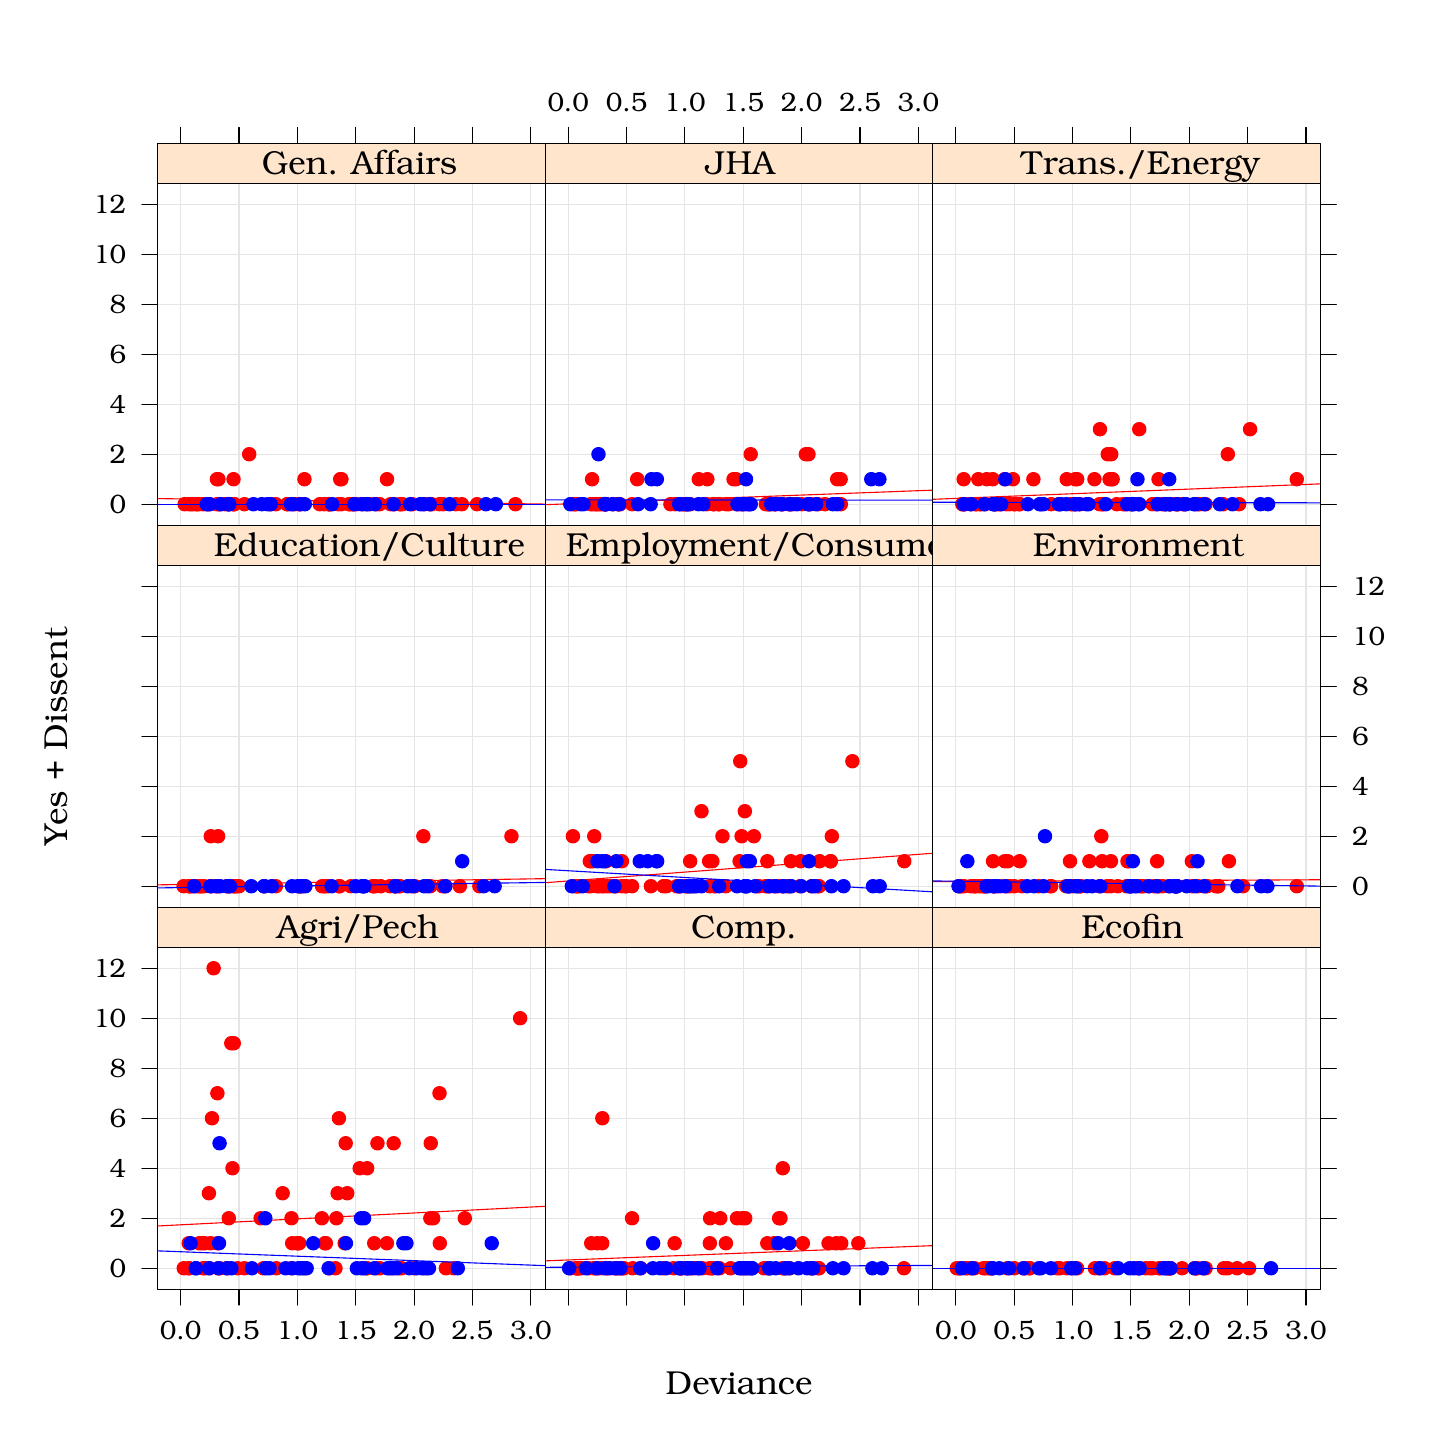
\begin{tikzpicture}[x=1pt,y=1pt]
\definecolor[named]{drawColor}{rgb}{0.00,0.00,0.00}
\definecolor[named]{fillColor}{rgb}{1.00,1.00,1.00}
\fill[color=fillColor,] (0,0) rectangle (505.89,505.89);
\begin{scope}
\path[clip] (  0.00,  0.00) rectangle (505.89,505.89);
\end{scope}
\begin{scope}
\path[clip] (  0.00,  0.00) rectangle (505.89,505.89);

\draw[fill opacity=0.00,draw opacity=0.00,] (  0.00,  0.00) rectangle (505.89,505.89);
\definecolor[named]{drawColor}{rgb}{0.00,0.00,0.00}

\node[color=drawColor,anchor=base,inner sep=0pt, outer sep=0pt, scale=  1.20] at (257.08, 12.04) {Deviance%
};
\end{scope}
\begin{scope}
\path[clip] (  0.00,  0.00) rectangle (505.89,505.89);
\definecolor[named]{drawColor}{rgb}{0.00,0.00,0.00}

\node[rotate= 90.00,color=drawColor,anchor=base,inner sep=0pt, outer sep=0pt, scale=  1.20] at ( 14.29,249.85) {Yes + Dissent%
};
\end{scope}
\begin{scope}
\path[clip] (  0.00,  0.00) rectangle (505.89,505.89);
\end{scope}
\begin{scope}
\path[clip] (  0.00,  0.00) rectangle (505.89,505.89);
\end{scope}
\begin{scope}
\path[clip] (  0.00,  0.00) rectangle (505.89,505.89);
\end{scope}
\begin{scope}
\path[clip] ( 46.98, 50.02) rectangle (187.04,173.60);
\end{scope}
\begin{scope}
\path[clip] (  0.00,  0.00) rectangle (505.89,505.89);
\end{scope}
\begin{scope}
\path[clip] (  0.00,  0.00) rectangle (505.89,505.89);
\end{scope}
\begin{scope}
\path[clip] (  0.00,  0.00) rectangle (505.89,505.89);
\end{scope}
\begin{scope}
\path[clip] (  0.00,  0.00) rectangle (505.89,505.89);
\definecolor[named]{drawColor}{rgb}{0.00,0.00,0.00}

\draw[color=drawColor,line cap=round,line join=round,fill opacity=0.00,] ( 46.98, 57.60) -- ( 41.29, 57.60);

\draw[color=drawColor,line cap=round,line join=round,fill opacity=0.00,] ( 46.98, 75.67) -- ( 41.29, 75.67);

\draw[color=drawColor,line cap=round,line join=round,fill opacity=0.00,] ( 46.98, 93.74) -- ( 41.29, 93.74);

\draw[color=drawColor,line cap=round,line join=round,fill opacity=0.00,] ( 46.98,111.81) -- ( 41.29,111.81);

\draw[color=drawColor,line cap=round,line join=round,fill opacity=0.00,] ( 46.98,129.88) -- ( 41.29,129.88);

\draw[color=drawColor,line cap=round,line join=round,fill opacity=0.00,] ( 46.98,147.95) -- ( 41.29,147.95);

\draw[color=drawColor,line cap=round,line join=round,fill opacity=0.00,] ( 46.98,166.01) -- ( 41.29,166.01);

\node[color=drawColor,anchor=base east,inner sep=0pt, outer sep=0pt, scale=  0.96] at ( 35.60, 54.30) {0%
};

\node[color=drawColor,anchor=base east,inner sep=0pt, outer sep=0pt, scale=  0.96] at ( 35.60, 72.37) {2%
};

\node[color=drawColor,anchor=base east,inner sep=0pt, outer sep=0pt, scale=  0.96] at ( 35.60, 90.43) {4%
};

\node[color=drawColor,anchor=base east,inner sep=0pt, outer sep=0pt, scale=  0.96] at ( 35.60,108.50) {6%
};

\node[color=drawColor,anchor=base east,inner sep=0pt, outer sep=0pt, scale=  0.96] at ( 35.60,126.57) {8%
};

\node[color=drawColor,anchor=base east,inner sep=0pt, outer sep=0pt, scale=  0.96] at ( 35.60,144.64) {10%
};

\node[color=drawColor,anchor=base east,inner sep=0pt, outer sep=0pt, scale=  0.96] at ( 35.60,162.71) {12%
};
\end{scope}
\begin{scope}
\path[clip] (  0.00,  0.00) rectangle (505.89,505.89);
\end{scope}
\begin{scope}
\path[clip] (  0.00,  0.00) rectangle (505.89,505.89);
\definecolor[named]{drawColor}{rgb}{0.00,0.00,0.00}

\draw[color=drawColor,line cap=round,line join=round,fill opacity=0.00,] ( 55.26, 50.02) -- ( 55.26, 44.32);

\draw[color=drawColor,line cap=round,line join=round,fill opacity=0.00,] ( 76.35, 50.02) -- ( 76.35, 44.32);

\draw[color=drawColor,line cap=round,line join=round,fill opacity=0.00,] ( 97.44, 50.02) -- ( 97.44, 44.32);

\draw[color=drawColor,line cap=round,line join=round,fill opacity=0.00,] (118.53, 50.02) -- (118.53, 44.32);

\draw[color=drawColor,line cap=round,line join=round,fill opacity=0.00,] (139.62, 50.02) -- (139.62, 44.32);

\draw[color=drawColor,line cap=round,line join=round,fill opacity=0.00,] (160.70, 50.02) -- (160.70, 44.32);

\draw[color=drawColor,line cap=round,line join=round,fill opacity=0.00,] (181.79, 50.02) -- (181.79, 44.32);

\node[color=drawColor,anchor=base,inner sep=0pt, outer sep=0pt, scale=  0.96] at ( 55.26, 32.02) {0.0%
};

\node[color=drawColor,anchor=base,inner sep=0pt, outer sep=0pt, scale=  0.96] at ( 76.35, 32.02) {0.5%
};

\node[color=drawColor,anchor=base,inner sep=0pt, outer sep=0pt, scale=  0.96] at ( 97.44, 32.02) {1.0%
};

\node[color=drawColor,anchor=base,inner sep=0pt, outer sep=0pt, scale=  0.96] at (118.53, 32.02) {1.5%
};

\node[color=drawColor,anchor=base,inner sep=0pt, outer sep=0pt, scale=  0.96] at (139.62, 32.02) {2.0%
};

\node[color=drawColor,anchor=base,inner sep=0pt, outer sep=0pt, scale=  0.96] at (160.70, 32.02) {2.5%
};

\node[color=drawColor,anchor=base,inner sep=0pt, outer sep=0pt, scale=  0.96] at (181.79, 32.02) {3.0%
};
\end{scope}
\begin{scope}
\path[clip] (  0.00,  0.00) rectangle (505.89,505.89);
\end{scope}
\begin{scope}
\path[clip] ( 46.98, 50.02) rectangle (187.04,173.60);
\definecolor[named]{drawColor}{rgb}{0.90,0.90,0.90}

\draw[color=drawColor,line cap=round,line join=round,fill opacity=0.00,] ( 46.98, 57.60) -- (187.04, 57.60);

\draw[color=drawColor,line cap=round,line join=round,fill opacity=0.00,] ( 46.98, 75.67) -- (187.04, 75.67);

\draw[color=drawColor,line cap=round,line join=round,fill opacity=0.00,] ( 46.98, 93.74) -- (187.04, 93.74);

\draw[color=drawColor,line cap=round,line join=round,fill opacity=0.00,] ( 46.98,111.81) -- (187.04,111.81);

\draw[color=drawColor,line cap=round,line join=round,fill opacity=0.00,] ( 46.98,129.88) -- (187.04,129.88);

\draw[color=drawColor,line cap=round,line join=round,fill opacity=0.00,] ( 46.98,147.95) -- (187.04,147.95);

\draw[color=drawColor,line cap=round,line join=round,fill opacity=0.00,] ( 46.98,166.01) -- (187.04,166.01);

\draw[color=drawColor,line cap=round,line join=round,fill opacity=0.00,] ( 55.26, 50.02) -- ( 55.26,173.60);

\draw[color=drawColor,line cap=round,line join=round,fill opacity=0.00,] ( 76.35, 50.02) -- ( 76.35,173.60);

\draw[color=drawColor,line cap=round,line join=round,fill opacity=0.00,] ( 97.44, 50.02) -- ( 97.44,173.60);

\draw[color=drawColor,line cap=round,line join=round,fill opacity=0.00,] (118.53, 50.02) -- (118.53,173.60);

\draw[color=drawColor,line cap=round,line join=round,fill opacity=0.00,] (139.62, 50.02) -- (139.62,173.60);

\draw[color=drawColor,line cap=round,line join=round,fill opacity=0.00,] (160.70, 50.02) -- (160.70,173.60);

\draw[color=drawColor,line cap=round,line join=round,fill opacity=0.00,] (181.79, 50.02) -- (181.79,173.60);
\definecolor[named]{drawColor}{rgb}{1.00,0.00,0.00}
\definecolor[named]{fillColor}{rgb}{1.00,0.00,0.00}

\draw[color=drawColor,line cap=round,line join=round,fill=fillColor,] ( 72.02, 57.60) circle (  2.41);

\draw[color=drawColor,line cap=round,line join=round,fill=fillColor,] ( 72.67, 75.67) circle (  2.41);

\draw[color=drawColor,line cap=round,line join=round,fill=fillColor,] ( 75.86, 57.60) circle (  2.41);

\draw[color=drawColor,line cap=round,line join=round,fill=fillColor,] (153.97, 57.60) circle (  2.41);

\draw[color=drawColor,line cap=round,line join=round,fill=fillColor,] ( 78.32, 57.60) circle (  2.41);

\draw[color=drawColor,line cap=round,line join=round,fill=fillColor,] (122.60, 57.60) circle (  2.41);

\draw[color=drawColor,line cap=round,line join=round,fill=fillColor,] ( 97.43, 66.64) circle (  2.41);

\draw[color=drawColor,line cap=round,line join=round,fill=fillColor,] ( 58.22, 57.60) circle (  2.41);

\draw[color=drawColor,line cap=round,line join=round,fill=fillColor,] ( 63.46, 57.60) circle (  2.41);

\draw[color=drawColor,line cap=round,line join=round,fill=fillColor,] ( 65.52, 57.60) circle (  2.41);

\draw[color=drawColor,line cap=round,line join=round,fill=fillColor,] ( 84.18, 75.67) circle (  2.41);

\draw[color=drawColor,line cap=round,line join=round,fill=fillColor,] ( 74.01, 93.74) circle (  2.41);

\draw[color=drawColor,line cap=round,line join=round,fill=fillColor,] ( 66.09, 66.64) circle (  2.41);

\draw[color=drawColor,line cap=round,line join=round,fill=fillColor,] ( 69.39, 57.60) circle (  2.41);

\draw[color=drawColor,line cap=round,line join=round,fill=fillColor,] (122.67, 93.74) circle (  2.41);

\draw[color=drawColor,line cap=round,line join=round,fill=fillColor,] (132.25,102.77) circle (  2.41);

\draw[color=drawColor,line cap=round,line join=round,fill=fillColor,] (131.67, 57.60) circle (  2.41);

\draw[color=drawColor,line cap=round,line join=round,fill=fillColor,] ( 65.49, 84.71) circle (  2.41);

\draw[color=drawColor,line cap=round,line join=round,fill=fillColor,] ( 85.14, 57.60) circle (  2.41);

\draw[color=drawColor,line cap=round,line join=round,fill=fillColor,] ( 62.04, 66.64) circle (  2.41);

\draw[color=drawColor,line cap=round,line join=round,fill=fillColor,] ( 95.24, 57.60) circle (  2.41);

\draw[color=drawColor,line cap=round,line join=round,fill=fillColor,] ( 68.59, 66.64) circle (  2.41);

\draw[color=drawColor,line cap=round,line join=round,fill=fillColor,] ( 68.90, 57.60) circle (  2.41);

\draw[color=drawColor,line cap=round,line join=round,fill=fillColor,] (139.66, 57.60) circle (  2.41);

\draw[color=drawColor,line cap=round,line join=round,fill=fillColor,] (143.13, 57.60) circle (  2.41);

\draw[color=drawColor,line cap=round,line join=round,fill=fillColor,] (146.54, 75.67) circle (  2.41);

\draw[color=drawColor,line cap=round,line join=round,fill=fillColor,] (100.06, 57.60) circle (  2.41);

\draw[color=drawColor,line cap=round,line join=round,fill=fillColor,] ( 95.59, 66.64) circle (  2.41);

\draw[color=drawColor,line cap=round,line join=round,fill=fillColor,] (111.56, 75.67) circle (  2.41);

\draw[color=drawColor,line cap=round,line join=round,fill=fillColor,] (114.92,102.77) circle (  2.41);

\draw[color=drawColor,line cap=round,line join=round,fill=fillColor,] ( 68.55,120.84) circle (  2.41);

\draw[color=drawColor,line cap=round,line join=round,fill=fillColor,] (119.97, 93.74) circle (  2.41);

\draw[color=drawColor,line cap=round,line join=round,fill=fillColor,] (157.96, 75.67) circle (  2.41);

\draw[color=drawColor,line cap=round,line join=round,fill=fillColor,] ( 97.65, 66.64) circle (  2.41);

\draw[color=drawColor,line cap=round,line join=round,fill=fillColor,] ( 98.11, 66.64) circle (  2.41);

\draw[color=drawColor,line cap=round,line join=round,fill=fillColor,] ( 63.05, 66.64) circle (  2.41);

\draw[color=drawColor,line cap=round,line join=round,fill=fillColor,] ( 95.34, 75.67) circle (  2.41);

\draw[color=drawColor,line cap=round,line join=round,fill=fillColor,] (148.92, 66.64) circle (  2.41);

\draw[color=drawColor,line cap=round,line join=round,fill=fillColor,] (115.49, 84.71) circle (  2.41);

\draw[color=drawColor,line cap=round,line join=round,fill=fillColor,] ( 58.24, 57.60) circle (  2.41);

\draw[color=drawColor,line cap=round,line join=round,fill=fillColor,] ( 56.40, 57.60) circle (  2.41);

\draw[color=drawColor,line cap=round,line join=round,fill=fillColor,] (145.51, 75.67) circle (  2.41);

\draw[color=drawColor,line cap=round,line join=round,fill=fillColor,] (122.46, 57.60) circle (  2.41);

\draw[color=drawColor,line cap=round,line join=round,fill=fillColor,] (125.89, 57.60) circle (  2.41);

\draw[color=drawColor,line cap=round,line join=round,fill=fillColor,] (134.26, 57.60) circle (  2.41);

\draw[color=drawColor,line cap=round,line join=round,fill=fillColor,] (135.11, 57.60) circle (  2.41);

\draw[color=drawColor,line cap=round,line join=round,fill=fillColor,] (151.13, 57.60) circle (  2.41);

\draw[color=drawColor,line cap=round,line join=round,fill=fillColor,] ( 89.88, 57.60) circle (  2.41);

\draw[color=drawColor,line cap=round,line join=round,fill=fillColor,] (129.79, 66.64) circle (  2.41);

\draw[color=drawColor,line cap=round,line join=round,fill=fillColor,] ( 58.18, 66.64) circle (  2.41);

\draw[color=drawColor,line cap=round,line join=round,fill=fillColor,] (111.22, 57.60) circle (  2.41);

\draw[color=drawColor,line cap=round,line join=round,fill=fillColor,] ( 66.60,111.81) circle (  2.41);

\draw[color=drawColor,line cap=round,line join=round,fill=fillColor,] ( 63.95, 66.64) circle (  2.41);

\draw[color=drawColor,line cap=round,line join=round,fill=fillColor,] ( 63.91, 57.60) circle (  2.41);

\draw[color=drawColor,line cap=round,line join=round,fill=fillColor,] ( 67.19,166.01) circle (  2.41);

\draw[color=drawColor,line cap=round,line join=round,fill=fillColor,] (109.14, 57.60) circle (  2.41);

\draw[color=drawColor,line cap=round,line join=round,fill=fillColor,] ( 74.47,138.91) circle (  2.41);

\draw[color=drawColor,line cap=round,line join=round,fill=fillColor,] ( 92.13, 84.71) circle (  2.41);

\draw[color=drawColor,line cap=round,line join=round,fill=fillColor,] (125.23, 66.64) circle (  2.41);

\draw[color=drawColor,line cap=round,line join=round,fill=fillColor,] (112.01, 84.71) circle (  2.41);

\draw[color=drawColor,line cap=round,line join=round,fill=fillColor,] (177.95,147.95) circle (  2.41);

\draw[color=drawColor,line cap=round,line join=round,fill=fillColor,] (145.65,102.77) circle (  2.41);

\draw[color=drawColor,line cap=round,line join=round,fill=fillColor,] (126.39,102.77) circle (  2.41);

\draw[color=drawColor,line cap=round,line join=round,fill=fillColor,] (127.24, 57.60) circle (  2.41);

\draw[color=drawColor,line cap=round,line join=round,fill=fillColor,] (114.55, 66.64) circle (  2.41);

\draw[color=drawColor,line cap=round,line join=round,fill=fillColor,] (148.82,120.84) circle (  2.41);

\draw[color=drawColor,line cap=round,line join=round,fill=fillColor,] (107.75, 66.64) circle (  2.41);

\draw[color=drawColor,line cap=round,line join=round,fill=fillColor,] ( 73.58,138.91) circle (  2.41);

\draw[color=drawColor,line cap=round,line join=round,fill=fillColor,] (112.48,111.81) circle (  2.41);

\draw[color=drawColor,line cap=round,line join=round,fill=fillColor,] (106.31, 75.67) circle (  2.41);

\draw[color=drawColor,line cap=round,line join=round,fill=fillColor,] (107.39, 66.64) circle (  2.41);

\draw[color=drawColor,line cap=round,line join=round,fill opacity=0.00,] (187.04, 79.99) --
	( 46.98, 72.88);
\definecolor[named]{drawColor}{rgb}{0.00,0.00,1.00}
\definecolor[named]{fillColor}{rgb}{0.00,0.00,1.00}

\draw[color=drawColor,line cap=round,line join=round,fill=fillColor,] ( 95.67, 57.60) circle (  2.41);

\draw[color=drawColor,line cap=round,line join=round,fill=fillColor,] (142.48, 57.60) circle (  2.41);

\draw[color=drawColor,line cap=round,line join=round,fill=fillColor,] (121.55, 75.67) circle (  2.41);

\draw[color=drawColor,line cap=round,line join=round,fill=fillColor,] ( 60.78, 57.60) circle (  2.41);

\draw[color=drawColor,line cap=round,line join=round,fill=fillColor,] ( 58.87, 66.64) circle (  2.41);

\draw[color=drawColor,line cap=round,line join=round,fill=fillColor,] ( 60.78, 57.60) circle (  2.41);

\draw[color=drawColor,line cap=round,line join=round,fill=fillColor,] (130.07, 57.60) circle (  2.41);

\draw[color=drawColor,line cap=round,line join=round,fill=fillColor,] ( 81.03, 57.60) circle (  2.41);

\draw[color=drawColor,line cap=round,line join=round,fill=fillColor,] ( 69.34,102.77) circle (  2.41);

\draw[color=drawColor,line cap=round,line join=round,fill=fillColor,] ( 99.54, 57.60) circle (  2.41);

\draw[color=drawColor,line cap=round,line join=round,fill=fillColor,] (103.17, 66.64) circle (  2.41);

\draw[color=drawColor,line cap=round,line join=round,fill=fillColor,] (140.57, 57.60) circle (  2.41);

\draw[color=drawColor,line cap=round,line join=round,fill=fillColor,] (167.68, 66.64) circle (  2.41);

\draw[color=drawColor,line cap=round,line join=round,fill=fillColor,] (136.87, 66.64) circle (  2.41);

\draw[color=drawColor,line cap=round,line join=round,fill=fillColor,] (137.96, 57.60) circle (  2.41);

\draw[color=drawColor,line cap=round,line join=round,fill=fillColor,] ( 93.20, 57.60) circle (  2.41);

\draw[color=drawColor,line cap=round,line join=round,fill=fillColor,] (120.69, 57.60) circle (  2.41);

\draw[color=drawColor,line cap=round,line join=round,fill=fillColor,] (100.81, 57.60) circle (  2.41);

\draw[color=drawColor,line cap=round,line join=round,fill=fillColor,] ( 97.86, 57.60) circle (  2.41);

\draw[color=drawColor,line cap=round,line join=round,fill=fillColor,] (118.97, 57.60) circle (  2.41);

\draw[color=drawColor,line cap=round,line join=round,fill=fillColor,] (121.56, 57.60) circle (  2.41);

\draw[color=drawColor,line cap=round,line join=round,fill=fillColor,] (120.43, 75.67) circle (  2.41);

\draw[color=drawColor,line cap=round,line join=round,fill=fillColor,] (125.32, 57.60) circle (  2.41);

\draw[color=drawColor,line cap=round,line join=round,fill=fillColor,] ( 69.13, 66.64) circle (  2.41);

\draw[color=drawColor,line cap=round,line join=round,fill=fillColor,] (144.09, 57.60) circle (  2.41);

\draw[color=drawColor,line cap=round,line join=round,fill=fillColor,] ( 85.87, 75.67) circle (  2.41);

\draw[color=drawColor,line cap=round,line join=round,fill=fillColor,] ( 87.38, 57.60) circle (  2.41);

\draw[color=drawColor,line cap=round,line join=round,fill=fillColor,] (135.77, 66.64) circle (  2.41);

\draw[color=drawColor,line cap=round,line join=round,fill=fillColor,] (132.18, 57.60) circle (  2.41);

\draw[color=drawColor,line cap=round,line join=round,fill=fillColor,] (155.42, 57.60) circle (  2.41);

\draw[color=drawColor,line cap=round,line join=round,fill=fillColor,] (144.99, 57.60) circle (  2.41);

\draw[color=drawColor,line cap=round,line join=round,fill=fillColor,] ( 65.62, 57.60) circle (  2.41);

\draw[color=drawColor,line cap=round,line join=round,fill=fillColor,] ( 98.56, 57.60) circle (  2.41);

\draw[color=drawColor,line cap=round,line join=round,fill=fillColor,] ( 68.94, 57.60) circle (  2.41);

\draw[color=drawColor,line cap=round,line join=round,fill=fillColor,] ( 72.03, 57.60) circle (  2.41);

\draw[color=drawColor,line cap=round,line join=round,fill=fillColor,] (115.01, 66.64) circle (  2.41);

\draw[color=drawColor,line cap=round,line join=round,fill=fillColor,] (108.74, 57.60) circle (  2.41);

\draw[color=drawColor,line cap=round,line join=round,fill=fillColor,] ( 73.61, 57.60) circle (  2.41);

\draw[color=drawColor,line cap=round,line join=round,fill=fillColor,] ( 86.05, 57.60) circle (  2.41);

\draw[color=drawColor,line cap=round,line join=round,fill=fillColor,] (133.40, 57.60) circle (  2.41);

\draw[color=drawColor,line cap=round,line join=round,fill=fillColor,] (130.77, 57.60) circle (  2.41);

\draw[color=drawColor,line cap=round,line join=round,fill opacity=0.00,] (187.04, 58.54) --
	( 46.98, 63.89);
\end{scope}
\begin{scope}
\path[clip] (  0.00,  0.00) rectangle (505.89,505.89);
\end{scope}
\begin{scope}
\path[clip] (  0.00,  0.00) rectangle (505.89,505.89);
\definecolor[named]{drawColor}{rgb}{0.00,0.00,0.00}

\draw[color=drawColor,line cap=round,line join=round,fill opacity=0.00,] ( 46.98, 50.02) rectangle (187.04,173.60);
\end{scope}
\begin{scope}
\path[clip] (  0.00,  0.00) rectangle (505.89,505.89);
\end{scope}
\begin{scope}
\path[clip] (  0.00,  0.00) rectangle (505.89,505.89);
\end{scope}
\begin{scope}
\path[clip] ( 46.98,173.60) rectangle (187.04,188.06);
\definecolor[named]{drawColor}{rgb}{1.00,0.90,0.80}
\definecolor[named]{fillColor}{rgb}{1.00,0.90,0.80}

\draw[color=drawColor,line cap=round,line join=round,fill=fillColor,] ( 46.98,173.60) rectangle (187.04,188.06);
\definecolor[named]{drawColor}{rgb}{0.00,0.00,0.00}

\node[color=drawColor,anchor=base west,inner sep=0pt, outer sep=0pt, scale=  1.20] at ( 90.09,176.70) {Agri/Pech%
};
\end{scope}
\begin{scope}
\path[clip] (  0.00,  0.00) rectangle (505.89,505.89);
\end{scope}
\begin{scope}
\path[clip] (  0.00,  0.00) rectangle (505.89,505.89);
\definecolor[named]{drawColor}{rgb}{0.00,0.00,0.00}

\draw[color=drawColor,line cap=round,line join=round,fill opacity=0.00,] ( 46.98,173.60) rectangle (187.04,188.06);
\end{scope}
\begin{scope}
\path[clip] (  0.00,  0.00) rectangle (505.89,505.89);
\end{scope}
\begin{scope}
\path[clip] (  0.00,  0.00) rectangle (505.89,505.89);
\end{scope}
\begin{scope}
\path[clip] (187.04, 50.02) rectangle (327.11,173.60);
\end{scope}
\begin{scope}
\path[clip] (  0.00,  0.00) rectangle (505.89,505.89);
\end{scope}
\begin{scope}
\path[clip] (  0.00,  0.00) rectangle (505.89,505.89);
\end{scope}
\begin{scope}
\path[clip] (  0.00,  0.00) rectangle (505.89,505.89);
\end{scope}
\begin{scope}
\path[clip] (  0.00,  0.00) rectangle (505.89,505.89);
\end{scope}
\begin{scope}
\path[clip] (  0.00,  0.00) rectangle (505.89,505.89);
\end{scope}
\begin{scope}
\path[clip] (  0.00,  0.00) rectangle (505.89,505.89);
\definecolor[named]{drawColor}{rgb}{0.00,0.00,0.00}

\draw[color=drawColor,line cap=round,line join=round,fill opacity=0.00,] (195.33, 50.02) -- (195.33, 44.32);

\draw[color=drawColor,line cap=round,line join=round,fill opacity=0.00,] (216.42, 50.02) -- (216.42, 44.32);

\draw[color=drawColor,line cap=round,line join=round,fill opacity=0.00,] (237.50, 50.02) -- (237.50, 44.32);

\draw[color=drawColor,line cap=round,line join=round,fill opacity=0.00,] (258.59, 50.02) -- (258.59, 44.32);

\draw[color=drawColor,line cap=round,line join=round,fill opacity=0.00,] (279.68, 50.02) -- (279.68, 44.32);

\draw[color=drawColor,line cap=round,line join=round,fill opacity=0.00,] (300.77, 50.02) -- (300.77, 44.32);

\draw[color=drawColor,line cap=round,line join=round,fill opacity=0.00,] (321.86, 50.02) -- (321.86, 44.32);
\end{scope}
\begin{scope}
\path[clip] (  0.00,  0.00) rectangle (505.89,505.89);
\end{scope}
\begin{scope}
\path[clip] (187.04, 50.02) rectangle (327.11,173.60);
\definecolor[named]{drawColor}{rgb}{0.90,0.90,0.90}

\draw[color=drawColor,line cap=round,line join=round,fill opacity=0.00,] (187.04, 57.60) -- (327.11, 57.60);

\draw[color=drawColor,line cap=round,line join=round,fill opacity=0.00,] (187.04, 75.67) -- (327.11, 75.67);

\draw[color=drawColor,line cap=round,line join=round,fill opacity=0.00,] (187.04, 93.74) -- (327.11, 93.74);

\draw[color=drawColor,line cap=round,line join=round,fill opacity=0.00,] (187.04,111.81) -- (327.11,111.81);

\draw[color=drawColor,line cap=round,line join=round,fill opacity=0.00,] (187.04,129.88) -- (327.11,129.88);

\draw[color=drawColor,line cap=round,line join=round,fill opacity=0.00,] (187.04,147.95) -- (327.11,147.95);

\draw[color=drawColor,line cap=round,line join=round,fill opacity=0.00,] (187.04,166.01) -- (327.11,166.01);

\draw[color=drawColor,line cap=round,line join=round,fill opacity=0.00,] (195.33, 50.02) -- (195.33,173.60);

\draw[color=drawColor,line cap=round,line join=round,fill opacity=0.00,] (216.42, 50.02) -- (216.42,173.60);

\draw[color=drawColor,line cap=round,line join=round,fill opacity=0.00,] (237.50, 50.02) -- (237.50,173.60);

\draw[color=drawColor,line cap=round,line join=round,fill opacity=0.00,] (258.59, 50.02) -- (258.59,173.60);

\draw[color=drawColor,line cap=round,line join=round,fill opacity=0.00,] (279.68, 50.02) -- (279.68,173.60);

\draw[color=drawColor,line cap=round,line join=round,fill opacity=0.00,] (300.77, 50.02) -- (300.77,173.60);

\draw[color=drawColor,line cap=round,line join=round,fill opacity=0.00,] (321.86, 50.02) -- (321.86,173.60);
\definecolor[named]{drawColor}{rgb}{1.00,0.00,0.00}
\definecolor[named]{fillColor}{rgb}{1.00,0.00,0.00}

\draw[color=drawColor,line cap=round,line join=round,fill=fillColor,] (212.83, 57.60) circle (  2.41);

\draw[color=drawColor,line cap=round,line join=round,fill=fillColor,] (212.09, 57.60) circle (  2.41);

\draw[color=drawColor,line cap=round,line join=round,fill=fillColor,] (215.50, 57.60) circle (  2.41);

\draw[color=drawColor,line cap=round,line join=round,fill=fillColor,] (280.10, 66.64) circle (  2.41);

\draw[color=drawColor,line cap=round,line join=round,fill=fillColor,] (218.39, 75.67) circle (  2.41);

\draw[color=drawColor,line cap=round,line join=round,fill=fillColor,] (259.69, 57.60) circle (  2.41);

\draw[color=drawColor,line cap=round,line join=round,fill=fillColor,] (236.45, 57.60) circle (  2.41);

\draw[color=drawColor,line cap=round,line join=round,fill=fillColor,] (198.29, 57.60) circle (  2.41);

\draw[color=drawColor,line cap=round,line join=round,fill=fillColor,] (202.68, 57.60) circle (  2.41);

\draw[color=drawColor,line cap=round,line join=round,fill=fillColor,] (206.03, 57.60) circle (  2.41);

\draw[color=drawColor,line cap=round,line join=round,fill=fillColor,] (241.05, 57.60) circle (  2.41);

\draw[color=drawColor,line cap=round,line join=round,fill=fillColor,] (218.62, 57.60) circle (  2.41);

\draw[color=drawColor,line cap=round,line join=round,fill=fillColor,] (207.62, 66.64) circle (  2.41);

\draw[color=drawColor,line cap=round,line join=round,fill=fillColor,] (209.42, 57.60) circle (  2.41);

\draw[color=drawColor,line cap=round,line join=round,fill=fillColor,] (258.11, 75.67) circle (  2.41);

\draw[color=drawColor,line cap=round,line join=round,fill=fillColor,] (272.03, 75.67) circle (  2.41);

\draw[color=drawColor,line cap=round,line join=round,fill=fillColor,] (271.54, 75.67) circle (  2.41);

\draw[color=drawColor,line cap=round,line join=round,fill=fillColor,] (272.79, 57.60) circle (  2.41);

\draw[color=drawColor,line cap=round,line join=round,fill=fillColor,] (205.84, 66.64) circle (  2.41);

\draw[color=drawColor,line cap=round,line join=round,fill=fillColor,] (221.50, 57.60) circle (  2.41);

\draw[color=drawColor,line cap=round,line join=round,fill=fillColor,] (199.44, 57.60) circle (  2.41);

\draw[color=drawColor,line cap=round,line join=round,fill=fillColor,] (207.41, 57.60) circle (  2.41);

\draw[color=drawColor,line cap=round,line join=round,fill=fillColor,] (235.95, 57.60) circle (  2.41);

\draw[color=drawColor,line cap=round,line join=round,fill=fillColor,] (213.13, 57.60) circle (  2.41);

\draw[color=drawColor,line cap=round,line join=round,fill=fillColor,] (209.37, 57.60) circle (  2.41);

\draw[color=drawColor,line cap=round,line join=round,fill=fillColor,] (283.25, 57.60) circle (  2.41);

\draw[color=drawColor,line cap=round,line join=round,fill=fillColor,] (289.40, 66.64) circle (  2.41);

\draw[color=drawColor,line cap=round,line join=round,fill=fillColor,] (239.49, 57.60) circle (  2.41);

\draw[color=drawColor,line cap=round,line join=round,fill=fillColor,] (235.78, 57.60) circle (  2.41);

\draw[color=drawColor,line cap=round,line join=round,fill=fillColor,] (243.80, 57.60) circle (  2.41);

\draw[color=drawColor,line cap=round,line join=round,fill=fillColor,] (253.98, 57.60) circle (  2.41);

\draw[color=drawColor,line cap=round,line join=round,fill=fillColor,] (207.66,111.81) circle (  2.41);

\draw[color=drawColor,line cap=round,line join=round,fill=fillColor,] (272.86, 93.74) circle (  2.41);

\draw[color=drawColor,line cap=round,line join=round,fill=fillColor,] (300.16, 66.64) circle (  2.41);

\draw[color=drawColor,line cap=round,line join=round,fill=fillColor,] (233.37, 57.60) circle (  2.41);

\draw[color=drawColor,line cap=round,line join=round,fill=fillColor,] (238.16, 57.60) circle (  2.41);

\draw[color=drawColor,line cap=round,line join=round,fill=fillColor,] (204.49, 57.60) circle (  2.41);

\draw[color=drawColor,line cap=round,line join=round,fill=fillColor,] (246.38, 57.60) circle (  2.41);

\draw[color=drawColor,line cap=round,line join=round,fill=fillColor,] (285.96, 57.60) circle (  2.41);

\draw[color=drawColor,line cap=round,line join=round,fill=fillColor,] (250.28, 75.67) circle (  2.41);

\draw[color=drawColor,line cap=round,line join=round,fill=fillColor,] (198.67, 57.60) circle (  2.41);

\draw[color=drawColor,line cap=round,line join=round,fill=fillColor,] (196.18, 57.60) circle (  2.41);

\draw[color=drawColor,line cap=round,line join=round,fill=fillColor,] (285.58, 57.60) circle (  2.41);

\draw[color=drawColor,line cap=round,line join=round,fill=fillColor,] (256.31, 75.67) circle (  2.41);

\draw[color=drawColor,line cap=round,line join=round,fill=fillColor,] (269.72, 66.64) circle (  2.41);

\draw[color=drawColor,line cap=round,line join=round,fill=fillColor,] (274.04, 57.60) circle (  2.41);

\draw[color=drawColor,line cap=round,line join=round,fill=fillColor,] (275.41, 57.60) circle (  2.41);

\draw[color=drawColor,line cap=round,line join=round,fill=fillColor,] (283.41, 57.60) circle (  2.41);

\draw[color=drawColor,line cap=round,line join=round,fill=fillColor,] (292.20, 66.64) circle (  2.41);

\draw[color=drawColor,line cap=round,line join=round,fill=fillColor,] (229.75, 57.60) circle (  2.41);

\draw[color=drawColor,line cap=round,line join=round,fill=fillColor,] (258.65, 57.60) circle (  2.41);

\draw[color=drawColor,line cap=round,line join=round,fill=fillColor,] (198.38, 57.60) circle (  2.41);

\draw[color=drawColor,line cap=round,line join=round,fill=fillColor,] (249.98, 57.60) circle (  2.41);

\draw[color=drawColor,line cap=round,line join=round,fill=fillColor,] (200.11, 57.60) circle (  2.41);

\draw[color=drawColor,line cap=round,line join=round,fill=fillColor,] (205.13, 57.60) circle (  2.41);

\draw[color=drawColor,line cap=round,line join=round,fill=fillColor,] (203.64, 66.64) circle (  2.41);

\draw[color=drawColor,line cap=round,line join=round,fill=fillColor,] (198.74, 57.60) circle (  2.41);

\draw[color=drawColor,line cap=round,line join=round,fill=fillColor,] (246.60, 75.67) circle (  2.41);

\draw[color=drawColor,line cap=round,line join=round,fill=fillColor,] (215.01, 57.60) circle (  2.41);

\draw[color=drawColor,line cap=round,line join=round,fill=fillColor,] (233.77, 66.64) circle (  2.41);

\draw[color=drawColor,line cap=round,line join=round,fill=fillColor,] (266.05, 57.60) circle (  2.41);

\draw[color=drawColor,line cap=round,line join=round,fill=fillColor,] (252.31, 66.64) circle (  2.41);

\draw[color=drawColor,line cap=round,line join=round,fill=fillColor,] (316.64, 57.60) circle (  2.41);

\draw[color=drawColor,line cap=round,line join=round,fill=fillColor,] (273.24, 57.60) circle (  2.41);

\draw[color=drawColor,line cap=round,line join=round,fill=fillColor,] (267.27, 66.64) circle (  2.41);

\draw[color=drawColor,line cap=round,line join=round,fill=fillColor,] (267.88, 57.60) circle (  2.41);

\draw[color=drawColor,line cap=round,line join=round,fill=fillColor,] (267.43, 57.60) circle (  2.41);

\draw[color=drawColor,line cap=round,line join=round,fill=fillColor,] (293.97, 66.64) circle (  2.41);

\draw[color=drawColor,line cap=round,line join=round,fill=fillColor,] (247.47, 57.60) circle (  2.41);

\draw[color=drawColor,line cap=round,line join=round,fill=fillColor,] (214.33, 57.60) circle (  2.41);

\draw[color=drawColor,line cap=round,line join=round,fill=fillColor,] (259.28, 75.67) circle (  2.41);

\draw[color=drawColor,line cap=round,line join=round,fill=fillColor,] (246.50, 66.64) circle (  2.41);

\draw[color=drawColor,line cap=round,line join=round,fill=fillColor,] (247.36, 57.60) circle (  2.41);

\draw[color=drawColor,line cap=round,line join=round,fill opacity=0.00,] (327.11, 65.78) --
	(187.04, 60.27);
\definecolor[named]{drawColor}{rgb}{0.00,0.00,1.00}
\definecolor[named]{fillColor}{rgb}{0.00,0.00,1.00}

\draw[color=drawColor,line cap=round,line join=round,fill=fillColor,] (235.40, 57.60) circle (  2.41);

\draw[color=drawColor,line cap=round,line join=round,fill=fillColor,] (283.26, 57.60) circle (  2.41);

\draw[color=drawColor,line cap=round,line join=round,fill=fillColor,] (261.72, 57.60) circle (  2.41);

\draw[color=drawColor,line cap=round,line join=round,fill=fillColor,] (238.48, 57.60) circle (  2.41);

\draw[color=drawColor,line cap=round,line join=round,fill=fillColor,] (201.77, 57.60) circle (  2.41);

\draw[color=drawColor,line cap=round,line join=round,fill=fillColor,] (195.65, 57.60) circle (  2.41);

\draw[color=drawColor,line cap=round,line join=round,fill=fillColor,] (270.30, 57.60) circle (  2.41);

\draw[color=drawColor,line cap=round,line join=round,fill=fillColor,] (221.37, 57.60) circle (  2.41);

\draw[color=drawColor,line cap=round,line join=round,fill=fillColor,] (210.44, 57.60) circle (  2.41);

\draw[color=drawColor,line cap=round,line join=round,fill=fillColor,] (239.94, 57.60) circle (  2.41);

\draw[color=drawColor,line cap=round,line join=round,fill=fillColor,] (290.96, 57.60) circle (  2.41);

\draw[color=drawColor,line cap=round,line join=round,fill=fillColor,] (242.31, 57.60) circle (  2.41);

\draw[color=drawColor,line cap=round,line join=round,fill=fillColor,] (305.25, 57.60) circle (  2.41);

\draw[color=drawColor,line cap=round,line join=round,fill=fillColor,] (281.64, 57.60) circle (  2.41);

\draw[color=drawColor,line cap=round,line join=round,fill=fillColor,] (308.59, 57.60) circle (  2.41);

\draw[color=drawColor,line cap=round,line join=round,fill=fillColor,] (275.12, 57.60) circle (  2.41);

\draw[color=drawColor,line cap=round,line join=round,fill=fillColor,] (261.15, 57.60) circle (  2.41);

\draw[color=drawColor,line cap=round,line join=round,fill=fillColor,] (236.15, 57.60) circle (  2.41);

\draw[color=drawColor,line cap=round,line join=round,fill=fillColor,] (260.17, 57.60) circle (  2.41);

\draw[color=drawColor,line cap=round,line join=round,fill=fillColor,] (242.75, 57.60) circle (  2.41);

\draw[color=drawColor,line cap=round,line join=round,fill=fillColor,] (230.70, 57.60) circle (  2.41);

\draw[color=drawColor,line cap=round,line join=round,fill=fillColor,] (258.88, 57.60) circle (  2.41);

\draw[color=drawColor,line cap=round,line join=round,fill=fillColor,] (261.80, 57.60) circle (  2.41);

\draw[color=drawColor,line cap=round,line join=round,fill=fillColor,] (257.84, 57.60) circle (  2.41);

\draw[color=drawColor,line cap=round,line join=round,fill=fillColor,] (268.25, 57.60) circle (  2.41);

\draw[color=drawColor,line cap=round,line join=round,fill=fillColor,] (208.66, 57.60) circle (  2.41);

\draw[color=drawColor,line cap=round,line join=round,fill=fillColor,] (283.79, 57.60) circle (  2.41);

\draw[color=drawColor,line cap=round,line join=round,fill=fillColor,] (226.01, 66.64) circle (  2.41);

\draw[color=drawColor,line cap=round,line join=round,fill=fillColor,] (228.49, 57.60) circle (  2.41);

\draw[color=drawColor,line cap=round,line join=round,fill=fillColor,] (275.21, 66.64) circle (  2.41);

\draw[color=drawColor,line cap=round,line join=round,fill=fillColor,] (271.18, 66.64) circle (  2.41);

\draw[color=drawColor,line cap=round,line join=round,fill=fillColor,] (294.81, 57.60) circle (  2.41);

\draw[color=drawColor,line cap=round,line join=round,fill=fillColor,] (278.53, 57.60) circle (  2.41);

\draw[color=drawColor,line cap=round,line join=round,fill=fillColor,] (205.77, 57.60) circle (  2.41);

\draw[color=drawColor,line cap=round,line join=round,fill=fillColor,] (238.19, 57.60) circle (  2.41);

\draw[color=drawColor,line cap=round,line join=round,fill=fillColor,] (212.57, 57.60) circle (  2.41);

\draw[color=drawColor,line cap=round,line join=round,fill=fillColor,] (257.15, 57.60) circle (  2.41);

\draw[color=drawColor,line cap=round,line join=round,fill=fillColor,] (249.17, 57.60) circle (  2.41);

\draw[color=drawColor,line cap=round,line join=round,fill=fillColor,] (214.20, 57.60) circle (  2.41);

\draw[color=drawColor,line cap=round,line join=round,fill=fillColor,] (225.92, 57.60) circle (  2.41);

\draw[color=drawColor,line cap=round,line join=round,fill=fillColor,] (273.83, 57.60) circle (  2.41);

\draw[color=drawColor,line cap=round,line join=round,fill=fillColor,] (267.95, 57.60) circle (  2.41);

\draw[color=drawColor,line cap=round,line join=round,fill opacity=0.00,] (327.11, 58.62) --
	(187.04, 57.94);
\end{scope}
\begin{scope}
\path[clip] (  0.00,  0.00) rectangle (505.89,505.89);
\end{scope}
\begin{scope}
\path[clip] (  0.00,  0.00) rectangle (505.89,505.89);
\definecolor[named]{drawColor}{rgb}{0.00,0.00,0.00}

\draw[color=drawColor,line cap=round,line join=round,fill opacity=0.00,] (187.04, 50.02) rectangle (327.11,173.60);
\end{scope}
\begin{scope}
\path[clip] (  0.00,  0.00) rectangle (505.89,505.89);
\end{scope}
\begin{scope}
\path[clip] (  0.00,  0.00) rectangle (505.89,505.89);
\end{scope}
\begin{scope}
\path[clip] (187.04,173.60) rectangle (327.11,188.06);
\definecolor[named]{drawColor}{rgb}{1.00,0.90,0.80}
\definecolor[named]{fillColor}{rgb}{1.00,0.90,0.80}

\draw[color=drawColor,line cap=round,line join=round,fill=fillColor,] (187.04,173.60) rectangle (327.11,188.06);
\definecolor[named]{drawColor}{rgb}{0.00,0.00,0.00}

\node[color=drawColor,anchor=base west,inner sep=0pt, outer sep=0pt, scale=  1.20] at (239.75,176.70) {Comp.%
};
\end{scope}
\begin{scope}
\path[clip] (  0.00,  0.00) rectangle (505.89,505.89);
\end{scope}
\begin{scope}
\path[clip] (  0.00,  0.00) rectangle (505.89,505.89);
\definecolor[named]{drawColor}{rgb}{0.00,0.00,0.00}

\draw[color=drawColor,line cap=round,line join=round,fill opacity=0.00,] (187.04,173.60) rectangle (327.11,188.06);
\end{scope}
\begin{scope}
\path[clip] (  0.00,  0.00) rectangle (505.89,505.89);
\end{scope}
\begin{scope}
\path[clip] (  0.00,  0.00) rectangle (505.89,505.89);
\end{scope}
\begin{scope}
\path[clip] (327.11, 50.02) rectangle (467.18,173.60);
\end{scope}
\begin{scope}
\path[clip] (  0.00,  0.00) rectangle (505.89,505.89);
\end{scope}
\begin{scope}
\path[clip] (  0.00,  0.00) rectangle (505.89,505.89);
\end{scope}
\begin{scope}
\path[clip] (  0.00,  0.00) rectangle (505.89,505.89);
\end{scope}
\begin{scope}
\path[clip] (  0.00,  0.00) rectangle (505.89,505.89);
\end{scope}
\begin{scope}
\path[clip] (  0.00,  0.00) rectangle (505.89,505.89);
\end{scope}
\begin{scope}
\path[clip] (  0.00,  0.00) rectangle (505.89,505.89);
\definecolor[named]{drawColor}{rgb}{0.00,0.00,0.00}

\draw[color=drawColor,line cap=round,line join=round,fill opacity=0.00,] (335.39, 50.02) -- (335.39, 44.32);

\draw[color=drawColor,line cap=round,line join=round,fill opacity=0.00,] (356.48, 50.02) -- (356.48, 44.32);

\draw[color=drawColor,line cap=round,line join=round,fill opacity=0.00,] (377.57, 50.02) -- (377.57, 44.32);

\draw[color=drawColor,line cap=round,line join=round,fill opacity=0.00,] (398.66, 50.02) -- (398.66, 44.32);

\draw[color=drawColor,line cap=round,line join=round,fill opacity=0.00,] (419.75, 50.02) -- (419.75, 44.32);

\draw[color=drawColor,line cap=round,line join=round,fill opacity=0.00,] (440.83, 50.02) -- (440.83, 44.32);

\draw[color=drawColor,line cap=round,line join=round,fill opacity=0.00,] (461.92, 50.02) -- (461.92, 44.32);

\node[color=drawColor,anchor=base,inner sep=0pt, outer sep=0pt, scale=  0.96] at (335.39, 32.02) {0.0%
};

\node[color=drawColor,anchor=base,inner sep=0pt, outer sep=0pt, scale=  0.96] at (356.48, 32.02) {0.5%
};

\node[color=drawColor,anchor=base,inner sep=0pt, outer sep=0pt, scale=  0.96] at (377.57, 32.02) {1.0%
};

\node[color=drawColor,anchor=base,inner sep=0pt, outer sep=0pt, scale=  0.96] at (398.66, 32.02) {1.5%
};

\node[color=drawColor,anchor=base,inner sep=0pt, outer sep=0pt, scale=  0.96] at (419.75, 32.02) {2.0%
};

\node[color=drawColor,anchor=base,inner sep=0pt, outer sep=0pt, scale=  0.96] at (440.83, 32.02) {2.5%
};

\node[color=drawColor,anchor=base,inner sep=0pt, outer sep=0pt, scale=  0.96] at (461.92, 32.02) {3.0%
};

\draw[color=drawColor,line cap=round,line join=round,fill opacity=0.00,] (467.18, 57.60) -- (472.87, 57.60);

\draw[color=drawColor,line cap=round,line join=round,fill opacity=0.00,] (467.18, 75.67) -- (472.87, 75.67);

\draw[color=drawColor,line cap=round,line join=round,fill opacity=0.00,] (467.18, 93.74) -- (472.87, 93.74);

\draw[color=drawColor,line cap=round,line join=round,fill opacity=0.00,] (467.18,111.81) -- (472.87,111.81);

\draw[color=drawColor,line cap=round,line join=round,fill opacity=0.00,] (467.18,129.88) -- (472.87,129.88);

\draw[color=drawColor,line cap=round,line join=round,fill opacity=0.00,] (467.18,147.95) -- (472.87,147.95);

\draw[color=drawColor,line cap=round,line join=round,fill opacity=0.00,] (467.18,166.01) -- (472.87,166.01);
\end{scope}
\begin{scope}
\path[clip] (  0.00,  0.00) rectangle (505.89,505.89);
\end{scope}
\begin{scope}
\path[clip] (327.11, 50.02) rectangle (467.18,173.60);
\definecolor[named]{drawColor}{rgb}{0.90,0.90,0.90}

\draw[color=drawColor,line cap=round,line join=round,fill opacity=0.00,] (327.11, 57.60) -- (467.18, 57.60);

\draw[color=drawColor,line cap=round,line join=round,fill opacity=0.00,] (327.11, 75.67) -- (467.18, 75.67);

\draw[color=drawColor,line cap=round,line join=round,fill opacity=0.00,] (327.11, 93.74) -- (467.18, 93.74);

\draw[color=drawColor,line cap=round,line join=round,fill opacity=0.00,] (327.11,111.81) -- (467.18,111.81);

\draw[color=drawColor,line cap=round,line join=round,fill opacity=0.00,] (327.11,129.88) -- (467.18,129.88);

\draw[color=drawColor,line cap=round,line join=round,fill opacity=0.00,] (327.11,147.95) -- (467.18,147.95);

\draw[color=drawColor,line cap=round,line join=round,fill opacity=0.00,] (327.11,166.01) -- (467.18,166.01);

\draw[color=drawColor,line cap=round,line join=round,fill opacity=0.00,] (335.39, 50.02) -- (335.39,173.60);

\draw[color=drawColor,line cap=round,line join=round,fill opacity=0.00,] (356.48, 50.02) -- (356.48,173.60);

\draw[color=drawColor,line cap=round,line join=round,fill opacity=0.00,] (377.57, 50.02) -- (377.57,173.60);

\draw[color=drawColor,line cap=round,line join=round,fill opacity=0.00,] (398.66, 50.02) -- (398.66,173.60);

\draw[color=drawColor,line cap=round,line join=round,fill opacity=0.00,] (419.75, 50.02) -- (419.75,173.60);

\draw[color=drawColor,line cap=round,line join=round,fill opacity=0.00,] (440.83, 50.02) -- (440.83,173.60);

\draw[color=drawColor,line cap=round,line join=round,fill opacity=0.00,] (461.92, 50.02) -- (461.92,173.60);
\definecolor[named]{drawColor}{rgb}{1.00,0.00,0.00}
\definecolor[named]{fillColor}{rgb}{1.00,0.00,0.00}

\draw[color=drawColor,line cap=round,line join=round,fill=fillColor,] (353.97, 57.60) circle (  2.41);

\draw[color=drawColor,line cap=round,line join=round,fill=fillColor,] (437.03, 57.60) circle (  2.41);

\draw[color=drawColor,line cap=round,line join=round,fill=fillColor,] (385.64, 57.60) circle (  2.41);

\draw[color=drawColor,line cap=round,line join=round,fill=fillColor,] (342.13, 57.60) circle (  2.41);

\draw[color=drawColor,line cap=round,line join=round,fill=fillColor,] (362.00, 57.60) circle (  2.41);

\draw[color=drawColor,line cap=round,line join=round,fill=fillColor,] (339.50, 57.60) circle (  2.41);

\draw[color=drawColor,line cap=round,line join=round,fill=fillColor,] (346.03, 57.60) circle (  2.41);

\draw[color=drawColor,line cap=round,line join=round,fill=fillColor,] (412.56, 57.60) circle (  2.41);

\draw[color=drawColor,line cap=round,line join=round,fill=fillColor,] (408.89, 57.60) circle (  2.41);

\draw[color=drawColor,line cap=round,line join=round,fill=fillColor,] (356.56, 57.60) circle (  2.41);

\draw[color=drawColor,line cap=round,line join=round,fill=fillColor,] (348.51, 57.60) circle (  2.41);

\draw[color=drawColor,line cap=round,line join=round,fill=fillColor,] (336.78, 57.60) circle (  2.41);

\draw[color=drawColor,line cap=round,line join=round,fill=fillColor,] (347.81, 57.60) circle (  2.41);

\draw[color=drawColor,line cap=round,line join=round,fill=fillColor,] (421.70, 57.60) circle (  2.41);

\draw[color=drawColor,line cap=round,line join=round,fill=fillColor,] (433.60, 57.60) circle (  2.41);

\draw[color=drawColor,line cap=round,line join=round,fill=fillColor,] (403.95, 57.60) circle (  2.41);

\draw[color=drawColor,line cap=round,line join=round,fill=fillColor,] (347.12, 57.60) circle (  2.41);

\draw[color=drawColor,line cap=round,line join=round,fill=fillColor,] (406.44, 57.60) circle (  2.41);

\draw[color=drawColor,line cap=round,line join=round,fill=fillColor,] (417.16, 57.60) circle (  2.41);

\draw[color=drawColor,line cap=round,line join=round,fill=fillColor,] (379.19, 57.60) circle (  2.41);

\draw[color=drawColor,line cap=round,line join=round,fill=fillColor,] (375.52, 57.60) circle (  2.41);

\draw[color=drawColor,line cap=round,line join=round,fill=fillColor,] (359.91, 57.60) circle (  2.41);

\draw[color=drawColor,line cap=round,line join=round,fill=fillColor,] (422.71, 57.60) circle (  2.41);

\draw[color=drawColor,line cap=round,line join=round,fill=fillColor,] (411.99, 57.60) circle (  2.41);

\draw[color=drawColor,line cap=round,line join=round,fill=fillColor,] (336.48, 57.60) circle (  2.41);

\draw[color=drawColor,line cap=round,line join=round,fill=fillColor,] (335.72, 57.60) circle (  2.41);

\draw[color=drawColor,line cap=round,line join=round,fill=fillColor,] (425.64, 57.60) circle (  2.41);

\draw[color=drawColor,line cap=round,line join=round,fill=fillColor,] (422.23, 57.60) circle (  2.41);

\draw[color=drawColor,line cap=round,line join=round,fill=fillColor,] (412.82, 57.60) circle (  2.41);

\draw[color=drawColor,line cap=round,line join=round,fill=fillColor,] (412.93, 57.60) circle (  2.41);

\draw[color=drawColor,line cap=round,line join=round,fill=fillColor,] (432.24, 57.60) circle (  2.41);

\draw[color=drawColor,line cap=round,line join=round,fill=fillColor,] (424.73, 57.60) circle (  2.41);

\draw[color=drawColor,line cap=round,line join=round,fill=fillColor,] (338.97, 57.60) circle (  2.41);

\draw[color=drawColor,line cap=round,line join=round,fill=fillColor,] (362.11, 57.60) circle (  2.41);

\draw[color=drawColor,line cap=round,line join=round,fill=fillColor,] (345.33, 57.60) circle (  2.41);

\draw[color=drawColor,line cap=round,line join=round,fill=fillColor,] (340.99, 57.60) circle (  2.41);

\draw[color=drawColor,line cap=round,line join=round,fill=fillColor,] (372.02, 57.60) circle (  2.41);

\draw[color=drawColor,line cap=round,line join=round,fill=fillColor,] (392.79, 57.60) circle (  2.41);

\draw[color=drawColor,line cap=round,line join=round,fill=fillColor,] (441.35, 57.60) circle (  2.41);

\draw[color=drawColor,line cap=round,line join=round,fill=fillColor,] (405.46, 57.60) circle (  2.41);

\draw[color=drawColor,line cap=round,line join=round,fill=fillColor,] (409.13, 57.60) circle (  2.41);

\draw[color=drawColor,line cap=round,line join=round,fill=fillColor,] (401.01, 57.60) circle (  2.41);

\draw[color=drawColor,line cap=round,line join=round,fill=fillColor,] (411.73, 57.60) circle (  2.41);

\draw[color=drawColor,line cap=round,line join=round,fill=fillColor,] (387.15, 57.60) circle (  2.41);

\draw[color=drawColor,line cap=round,line join=round,fill=fillColor,] (360.31, 57.60) circle (  2.41);

\draw[color=drawColor,line cap=round,line join=round,fill=fillColor,] (372.96, 57.60) circle (  2.41);

\draw[color=drawColor,line cap=round,line join=round,fill=fillColor,] (377.36, 57.60) circle (  2.41);

\draw[color=drawColor,line cap=round,line join=round,fill=fillColor,] (389.09, 57.60) circle (  2.41);

\draw[color=drawColor,line cap=round,line join=round,fill opacity=0.00,] (467.18, 57.60) --
	(327.11, 57.60);
\definecolor[named]{drawColor}{rgb}{0.00,0.00,1.00}
\definecolor[named]{fillColor}{rgb}{0.00,0.00,1.00}

\draw[color=drawColor,line cap=round,line join=round,fill=fillColor,] (377.08, 57.60) circle (  2.41);

\draw[color=drawColor,line cap=round,line join=round,fill=fillColor,] (424.83, 57.60) circle (  2.41);

\draw[color=drawColor,line cap=round,line join=round,fill=fillColor,] (401.74, 57.60) circle (  2.41);

\draw[color=drawColor,line cap=round,line join=round,fill=fillColor,] (337.54, 57.60) circle (  2.41);

\draw[color=drawColor,line cap=round,line join=round,fill=fillColor,] (359.88, 57.60) circle (  2.41);

\draw[color=drawColor,line cap=round,line join=round,fill=fillColor,] (341.38, 57.60) circle (  2.41);

\draw[color=drawColor,line cap=round,line join=round,fill=fillColor,] (378.46, 57.60) circle (  2.41);

\draw[color=drawColor,line cap=round,line join=round,fill=fillColor,] (421.68, 57.60) circle (  2.41);

\draw[color=drawColor,line cap=round,line join=round,fill=fillColor,] (449.28, 57.60) circle (  2.41);

\draw[color=drawColor,line cap=round,line join=round,fill=fillColor,] (410.43, 57.60) circle (  2.41);

\draw[color=drawColor,line cap=round,line join=round,fill=fillColor,] (398.20, 57.60) circle (  2.41);

\draw[color=drawColor,line cap=round,line join=round,fill=fillColor,] (387.52, 57.60) circle (  2.41);

\draw[color=drawColor,line cap=round,line join=round,fill=fillColor,] (399.62, 57.60) circle (  2.41);

\draw[color=drawColor,line cap=round,line join=round,fill=fillColor,] (393.98, 57.60) circle (  2.41);

\draw[color=drawColor,line cap=round,line join=round,fill=fillColor,] (348.47, 57.60) circle (  2.41);

\draw[color=drawColor,line cap=round,line join=round,fill=fillColor,] (366.06, 57.60) circle (  2.41);

\draw[color=drawColor,line cap=round,line join=round,fill=fillColor,] (369.73, 57.60) circle (  2.41);

\draw[color=drawColor,line cap=round,line join=round,fill=fillColor,] (411.28, 57.60) circle (  2.41);

\draw[color=drawColor,line cap=round,line join=round,fill=fillColor,] (412.97, 57.60) circle (  2.41);

\draw[color=drawColor,line cap=round,line join=round,fill=fillColor,] (348.66, 57.60) circle (  2.41);

\draw[color=drawColor,line cap=round,line join=round,fill=fillColor,] (351.13, 57.60) circle (  2.41);

\draw[color=drawColor,line cap=round,line join=round,fill=fillColor,] (401.75, 57.60) circle (  2.41);

\draw[color=drawColor,line cap=round,line join=round,fill=fillColor,] (354.65, 57.60) circle (  2.41);

\draw[color=drawColor,line cap=round,line join=round,fill=fillColor,] (365.39, 57.60) circle (  2.41);

\draw[color=drawColor,line cap=round,line join=round,fill opacity=0.00,] (467.18, 57.60) --
	(327.11, 57.60);
\end{scope}
\begin{scope}
\path[clip] (  0.00,  0.00) rectangle (505.89,505.89);
\end{scope}
\begin{scope}
\path[clip] (  0.00,  0.00) rectangle (505.89,505.89);
\definecolor[named]{drawColor}{rgb}{0.00,0.00,0.00}

\draw[color=drawColor,line cap=round,line join=round,fill opacity=0.00,] (327.11, 50.02) rectangle (467.18,173.60);
\end{scope}
\begin{scope}
\path[clip] (  0.00,  0.00) rectangle (505.89,505.89);
\end{scope}
\begin{scope}
\path[clip] (  0.00,  0.00) rectangle (505.89,505.89);
\end{scope}
\begin{scope}
\path[clip] (327.11,173.60) rectangle (467.18,188.06);
\definecolor[named]{drawColor}{rgb}{1.00,0.90,0.80}
\definecolor[named]{fillColor}{rgb}{1.00,0.90,0.80}

\draw[color=drawColor,line cap=round,line join=round,fill=fillColor,] (327.11,173.60) rectangle (467.18,188.06);
\definecolor[named]{drawColor}{rgb}{0.00,0.00,0.00}

\node[color=drawColor,anchor=base west,inner sep=0pt, outer sep=0pt, scale=  1.20] at (380.73,176.70) {Ecofin%
};
\end{scope}
\begin{scope}
\path[clip] (  0.00,  0.00) rectangle (505.89,505.89);
\end{scope}
\begin{scope}
\path[clip] (  0.00,  0.00) rectangle (505.89,505.89);
\definecolor[named]{drawColor}{rgb}{0.00,0.00,0.00}

\draw[color=drawColor,line cap=round,line join=round,fill opacity=0.00,] (327.11,173.60) rectangle (467.18,188.06);
\end{scope}
\begin{scope}
\path[clip] (  0.00,  0.00) rectangle (505.89,505.89);
\end{scope}
\begin{scope}
\path[clip] (  0.00,  0.00) rectangle (505.89,505.89);
\end{scope}
\begin{scope}
\path[clip] ( 46.98,188.06) rectangle (187.04,311.64);
\end{scope}
\begin{scope}
\path[clip] (  0.00,  0.00) rectangle (505.89,505.89);
\end{scope}
\begin{scope}
\path[clip] (  0.00,  0.00) rectangle (505.89,505.89);
\end{scope}
\begin{scope}
\path[clip] (  0.00,  0.00) rectangle (505.89,505.89);
\end{scope}
\begin{scope}
\path[clip] (  0.00,  0.00) rectangle (505.89,505.89);
\definecolor[named]{drawColor}{rgb}{0.00,0.00,0.00}

\draw[color=drawColor,line cap=round,line join=round,fill opacity=0.00,] ( 46.98,195.65) -- ( 41.29,195.65);

\draw[color=drawColor,line cap=round,line join=round,fill opacity=0.00,] ( 46.98,213.71) -- ( 41.29,213.71);

\draw[color=drawColor,line cap=round,line join=round,fill opacity=0.00,] ( 46.98,231.78) -- ( 41.29,231.78);

\draw[color=drawColor,line cap=round,line join=round,fill opacity=0.00,] ( 46.98,249.85) -- ( 41.29,249.85);

\draw[color=drawColor,line cap=round,line join=round,fill opacity=0.00,] ( 46.98,267.92) -- ( 41.29,267.92);

\draw[color=drawColor,line cap=round,line join=round,fill opacity=0.00,] ( 46.98,285.99) -- ( 41.29,285.99);

\draw[color=drawColor,line cap=round,line join=round,fill opacity=0.00,] ( 46.98,304.06) -- ( 41.29,304.06);
\end{scope}
\begin{scope}
\path[clip] (  0.00,  0.00) rectangle (505.89,505.89);
\end{scope}
\begin{scope}
\path[clip] (  0.00,  0.00) rectangle (505.89,505.89);
\end{scope}
\begin{scope}
\path[clip] (  0.00,  0.00) rectangle (505.89,505.89);
\end{scope}
\begin{scope}
\path[clip] ( 46.98,188.06) rectangle (187.04,311.64);
\definecolor[named]{drawColor}{rgb}{0.90,0.90,0.90}

\draw[color=drawColor,line cap=round,line join=round,fill opacity=0.00,] ( 46.98,195.65) -- (187.04,195.65);

\draw[color=drawColor,line cap=round,line join=round,fill opacity=0.00,] ( 46.98,213.71) -- (187.04,213.71);

\draw[color=drawColor,line cap=round,line join=round,fill opacity=0.00,] ( 46.98,231.78) -- (187.04,231.78);

\draw[color=drawColor,line cap=round,line join=round,fill opacity=0.00,] ( 46.98,249.85) -- (187.04,249.85);

\draw[color=drawColor,line cap=round,line join=round,fill opacity=0.00,] ( 46.98,267.92) -- (187.04,267.92);

\draw[color=drawColor,line cap=round,line join=round,fill opacity=0.00,] ( 46.98,285.99) -- (187.04,285.99);

\draw[color=drawColor,line cap=round,line join=round,fill opacity=0.00,] ( 46.98,304.06) -- (187.04,304.06);

\draw[color=drawColor,line cap=round,line join=round,fill opacity=0.00,] ( 55.26,188.06) -- ( 55.26,311.64);

\draw[color=drawColor,line cap=round,line join=round,fill opacity=0.00,] ( 76.35,188.06) -- ( 76.35,311.64);

\draw[color=drawColor,line cap=round,line join=round,fill opacity=0.00,] ( 97.44,188.06) -- ( 97.44,311.64);

\draw[color=drawColor,line cap=round,line join=round,fill opacity=0.00,] (118.53,188.06) -- (118.53,311.64);

\draw[color=drawColor,line cap=round,line join=round,fill opacity=0.00,] (139.62,188.06) -- (139.62,311.64);

\draw[color=drawColor,line cap=round,line join=round,fill opacity=0.00,] (160.70,188.06) -- (160.70,311.64);

\draw[color=drawColor,line cap=round,line join=round,fill opacity=0.00,] (181.79,188.06) -- (181.79,311.64);
\definecolor[named]{drawColor}{rgb}{1.00,0.00,0.00}
\definecolor[named]{fillColor}{rgb}{1.00,0.00,0.00}

\draw[color=drawColor,line cap=round,line join=round,fill=fillColor,] ( 71.98,195.65) circle (  2.41);

\draw[color=drawColor,line cap=round,line join=round,fill=fillColor,] ( 72.61,195.65) circle (  2.41);

\draw[color=drawColor,line cap=round,line join=round,fill=fillColor,] ( 76.36,195.65) circle (  2.41);

\draw[color=drawColor,line cap=round,line join=round,fill=fillColor,] (163.23,195.65) circle (  2.41);

\draw[color=drawColor,line cap=round,line join=round,fill=fillColor,] ( 98.47,195.65) circle (  2.41);

\draw[color=drawColor,line cap=round,line join=round,fill=fillColor,] ( 58.22,195.65) circle (  2.41);

\draw[color=drawColor,line cap=round,line join=round,fill=fillColor,] ( 62.41,195.65) circle (  2.41);

\draw[color=drawColor,line cap=round,line join=round,fill=fillColor,] ( 66.37,195.65) circle (  2.41);

\draw[color=drawColor,line cap=round,line join=round,fill=fillColor,] ( 75.54,195.65) circle (  2.41);

\draw[color=drawColor,line cap=round,line join=round,fill=fillColor,] ( 66.41,195.65) circle (  2.41);

\draw[color=drawColor,line cap=round,line join=round,fill=fillColor,] ( 68.10,195.65) circle (  2.41);

\draw[color=drawColor,line cap=round,line join=round,fill=fillColor,] (132.29,195.65) circle (  2.41);

\draw[color=drawColor,line cap=round,line join=round,fill=fillColor,] (130.90,195.65) circle (  2.41);

\draw[color=drawColor,line cap=round,line join=round,fill=fillColor,] (133.13,195.65) circle (  2.41);

\draw[color=drawColor,line cap=round,line join=round,fill=fillColor,] ( 62.84,195.65) circle (  2.41);

\draw[color=drawColor,line cap=round,line join=round,fill=fillColor,] ( 59.37,195.65) circle (  2.41);

\draw[color=drawColor,line cap=round,line join=round,fill=fillColor,] ( 62.05,195.65) circle (  2.41);

\draw[color=drawColor,line cap=round,line join=round,fill=fillColor,] ( 60.92,195.65) circle (  2.41);

\draw[color=drawColor,line cap=round,line join=round,fill=fillColor,] ( 69.09,195.65) circle (  2.41);

\draw[color=drawColor,line cap=round,line join=round,fill=fillColor,] (142.98,213.71) circle (  2.41);

\draw[color=drawColor,line cap=round,line join=round,fill=fillColor,] (139.88,195.65) circle (  2.41);

\draw[color=drawColor,line cap=round,line join=round,fill=fillColor,] (116.78,195.65) circle (  2.41);

\draw[color=drawColor,line cap=round,line join=round,fill=fillColor,] ( 68.81,213.71) circle (  2.41);

\draw[color=drawColor,line cap=round,line join=round,fill=fillColor,] (112.72,195.65) circle (  2.41);

\draw[color=drawColor,line cap=round,line join=round,fill=fillColor,] ( 98.91,195.65) circle (  2.41);

\draw[color=drawColor,line cap=round,line join=round,fill=fillColor,] ( 97.90,195.65) circle (  2.41);

\draw[color=drawColor,line cap=round,line join=round,fill=fillColor,] ( 66.18,213.71) circle (  2.41);

\draw[color=drawColor,line cap=round,line join=round,fill=fillColor,] (156.17,195.65) circle (  2.41);

\draw[color=drawColor,line cap=round,line join=round,fill=fillColor,] (124.82,195.65) circle (  2.41);

\draw[color=drawColor,line cap=round,line join=round,fill=fillColor,] ( 58.56,195.65) circle (  2.41);

\draw[color=drawColor,line cap=round,line join=round,fill=fillColor,] ( 56.34,195.65) circle (  2.41);

\draw[color=drawColor,line cap=round,line join=round,fill=fillColor,] (125.64,195.65) circle (  2.41);

\draw[color=drawColor,line cap=round,line join=round,fill=fillColor,] (134.20,195.65) circle (  2.41);

\draw[color=drawColor,line cap=round,line join=round,fill=fillColor,] (134.61,195.65) circle (  2.41);

\draw[color=drawColor,line cap=round,line join=round,fill=fillColor,] (145.51,195.65) circle (  2.41);

\draw[color=drawColor,line cap=round,line join=round,fill=fillColor,] (149.90,195.65) circle (  2.41);

\draw[color=drawColor,line cap=round,line join=round,fill=fillColor,] ( 89.68,195.65) circle (  2.41);

\draw[color=drawColor,line cap=round,line join=round,fill=fillColor,] (150.93,195.65) circle (  2.41);

\draw[color=drawColor,line cap=round,line join=round,fill=fillColor,] ( 58.69,195.65) circle (  2.41);

\draw[color=drawColor,line cap=round,line join=round,fill=fillColor,] ( 74.93,195.65) circle (  2.41);

\draw[color=drawColor,line cap=round,line join=round,fill=fillColor,] ( 63.78,195.65) circle (  2.41);

\draw[color=drawColor,line cap=round,line join=round,fill=fillColor,] ( 74.45,195.65) circle (  2.41);

\draw[color=drawColor,line cap=round,line join=round,fill=fillColor,] ( 74.67,195.65) circle (  2.41);

\draw[color=drawColor,line cap=round,line join=round,fill=fillColor,] ( 85.57,195.65) circle (  2.41);

\draw[color=drawColor,line cap=round,line join=round,fill=fillColor,] (112.52,195.65) circle (  2.41);

\draw[color=drawColor,line cap=round,line join=round,fill=fillColor,] (174.81,213.71) circle (  2.41);

\draw[color=drawColor,line cap=round,line join=round,fill=fillColor,] (124.87,195.65) circle (  2.41);

\draw[color=drawColor,line cap=round,line join=round,fill=fillColor,] (127.59,195.65) circle (  2.41);

\draw[color=drawColor,line cap=round,line join=round,fill=fillColor,] (107.29,195.65) circle (  2.41);

\draw[color=drawColor,line cap=round,line join=round,fill=fillColor,] (138.64,195.65) circle (  2.41);

\draw[color=drawColor,line cap=round,line join=round,fill=fillColor,] (108.43,195.65) circle (  2.41);

\draw[color=drawColor,line cap=round,line join=round,fill=fillColor,] ( 72.92,195.65) circle (  2.41);

\draw[color=drawColor,line cap=round,line join=round,fill=fillColor,] (106.38,195.65) circle (  2.41);

\draw[color=drawColor,line cap=round,line join=round,fill=fillColor,] (107.39,195.65) circle (  2.41);

\draw[color=drawColor,line cap=round,line join=round,fill opacity=0.00,] (187.04,198.39) --
	( 46.98,196.14);
\definecolor[named]{drawColor}{rgb}{0.00,0.00,1.00}
\definecolor[named]{fillColor}{rgb}{0.00,0.00,1.00}

\draw[color=drawColor,line cap=round,line join=round,fill=fillColor,] ( 95.54,195.65) circle (  2.41);

\draw[color=drawColor,line cap=round,line join=round,fill=fillColor,] (143.30,195.65) circle (  2.41);

\draw[color=drawColor,line cap=round,line join=round,fill=fillColor,] (121.15,195.65) circle (  2.41);

\draw[color=drawColor,line cap=round,line join=round,fill=fillColor,] ( 98.41,195.65) circle (  2.41);

\draw[color=drawColor,line cap=round,line join=round,fill=fillColor,] ( 60.15,195.65) circle (  2.41);

\draw[color=drawColor,line cap=round,line join=round,fill=fillColor,] ( 80.83,195.65) circle (  2.41);

\draw[color=drawColor,line cap=round,line join=round,fill=fillColor,] ( 68.29,195.65) circle (  2.41);

\draw[color=drawColor,line cap=round,line join=round,fill=fillColor,] ( 99.40,195.65) circle (  2.41);

\draw[color=drawColor,line cap=round,line join=round,fill=fillColor,] (150.89,195.65) circle (  2.41);

\draw[color=drawColor,line cap=round,line join=round,fill=fillColor,] (164.78,195.65) circle (  2.41);

\draw[color=drawColor,line cap=round,line join=round,fill=fillColor,] (139.34,195.65) circle (  2.41);

\draw[color=drawColor,line cap=round,line join=round,fill=fillColor,] (168.74,195.65) circle (  2.41);

\draw[color=drawColor,line cap=round,line join=round,fill=fillColor,] (137.34,195.65) circle (  2.41);

\draw[color=drawColor,line cap=round,line join=round,fill=fillColor,] (121.49,195.65) circle (  2.41);

\draw[color=drawColor,line cap=round,line join=round,fill=fillColor,] (118.48,195.65) circle (  2.41);

\draw[color=drawColor,line cap=round,line join=round,fill=fillColor,] (100.35,195.65) circle (  2.41);

\draw[color=drawColor,line cap=round,line join=round,fill=fillColor,] (121.69,195.65) circle (  2.41);

\draw[color=drawColor,line cap=round,line join=round,fill=fillColor,] (120.89,195.65) circle (  2.41);

\draw[color=drawColor,line cap=round,line join=round,fill=fillColor,] ( 69.57,195.65) circle (  2.41);

\draw[color=drawColor,line cap=round,line join=round,fill=fillColor,] (144.51,195.65) circle (  2.41);

\draw[color=drawColor,line cap=round,line join=round,fill=fillColor,] ( 85.47,195.65) circle (  2.41);

\draw[color=drawColor,line cap=round,line join=round,fill=fillColor,] ( 88.20,195.65) circle (  2.41);

\draw[color=drawColor,line cap=round,line join=round,fill=fillColor,] (132.84,195.65) circle (  2.41);

\draw[color=drawColor,line cap=round,line join=round,fill=fillColor,] (157.02,204.68) circle (  2.41);

\draw[color=drawColor,line cap=round,line join=round,fill=fillColor,] ( 66.01,195.65) circle (  2.41);

\draw[color=drawColor,line cap=round,line join=round,fill=fillColor,] ( 97.71,195.65) circle (  2.41);

\draw[color=drawColor,line cap=round,line join=round,fill=fillColor,] ( 72.07,195.65) circle (  2.41);

\draw[color=drawColor,line cap=round,line join=round,fill=fillColor,] (109.81,195.65) circle (  2.41);

\draw[color=drawColor,line cap=round,line join=round,fill=fillColor,] ( 73.11,195.65) circle (  2.41);

\draw[color=drawColor,line cap=round,line join=round,fill=fillColor,] ( 85.39,195.65) circle (  2.41);

\draw[color=drawColor,line cap=round,line join=round,fill=fillColor,] (132.98,195.65) circle (  2.41);

\draw[color=drawColor,line cap=round,line join=round,fill opacity=0.00,] (187.04,197.02) --
	( 46.98,195.04);
\end{scope}
\begin{scope}
\path[clip] (  0.00,  0.00) rectangle (505.89,505.89);
\end{scope}
\begin{scope}
\path[clip] (  0.00,  0.00) rectangle (505.89,505.89);
\definecolor[named]{drawColor}{rgb}{0.00,0.00,0.00}

\draw[color=drawColor,line cap=round,line join=round,fill opacity=0.00,] ( 46.98,188.06) rectangle (187.04,311.64);
\end{scope}
\begin{scope}
\path[clip] (  0.00,  0.00) rectangle (505.89,505.89);
\end{scope}
\begin{scope}
\path[clip] (  0.00,  0.00) rectangle (505.89,505.89);
\end{scope}
\begin{scope}
\path[clip] ( 46.98,311.64) rectangle (187.04,326.10);
\definecolor[named]{drawColor}{rgb}{1.00,0.90,0.80}
\definecolor[named]{fillColor}{rgb}{1.00,0.90,0.80}

\draw[color=drawColor,line cap=round,line join=round,fill=fillColor,] ( 46.98,311.64) rectangle (187.04,326.10);
\definecolor[named]{drawColor}{rgb}{0.00,0.00,0.00}

\node[color=drawColor,anchor=base west,inner sep=0pt, outer sep=0pt, scale=  1.20] at ( 67.26,314.74) {Education/Culture%
};
\end{scope}
\begin{scope}
\path[clip] (  0.00,  0.00) rectangle (505.89,505.89);
\end{scope}
\begin{scope}
\path[clip] (  0.00,  0.00) rectangle (505.89,505.89);
\definecolor[named]{drawColor}{rgb}{0.00,0.00,0.00}

\draw[color=drawColor,line cap=round,line join=round,fill opacity=0.00,] ( 46.98,311.64) rectangle (187.04,326.10);
\end{scope}
\begin{scope}
\path[clip] (  0.00,  0.00) rectangle (505.89,505.89);
\end{scope}
\begin{scope}
\path[clip] (  0.00,  0.00) rectangle (505.89,505.89);
\end{scope}
\begin{scope}
\path[clip] (187.04,188.06) rectangle (327.11,311.64);
\end{scope}
\begin{scope}
\path[clip] (  0.00,  0.00) rectangle (505.89,505.89);
\end{scope}
\begin{scope}
\path[clip] (  0.00,  0.00) rectangle (505.89,505.89);
\end{scope}
\begin{scope}
\path[clip] (  0.00,  0.00) rectangle (505.89,505.89);
\end{scope}
\begin{scope}
\path[clip] (  0.00,  0.00) rectangle (505.89,505.89);
\end{scope}
\begin{scope}
\path[clip] (  0.00,  0.00) rectangle (505.89,505.89);
\end{scope}
\begin{scope}
\path[clip] (  0.00,  0.00) rectangle (505.89,505.89);
\end{scope}
\begin{scope}
\path[clip] (  0.00,  0.00) rectangle (505.89,505.89);
\end{scope}
\begin{scope}
\path[clip] (187.04,188.06) rectangle (327.11,311.64);
\definecolor[named]{drawColor}{rgb}{0.90,0.90,0.90}

\draw[color=drawColor,line cap=round,line join=round,fill opacity=0.00,] (187.04,195.65) -- (327.11,195.65);

\draw[color=drawColor,line cap=round,line join=round,fill opacity=0.00,] (187.04,213.71) -- (327.11,213.71);

\draw[color=drawColor,line cap=round,line join=round,fill opacity=0.00,] (187.04,231.78) -- (327.11,231.78);

\draw[color=drawColor,line cap=round,line join=round,fill opacity=0.00,] (187.04,249.85) -- (327.11,249.85);

\draw[color=drawColor,line cap=round,line join=round,fill opacity=0.00,] (187.04,267.92) -- (327.11,267.92);

\draw[color=drawColor,line cap=round,line join=round,fill opacity=0.00,] (187.04,285.99) -- (327.11,285.99);

\draw[color=drawColor,line cap=round,line join=round,fill opacity=0.00,] (187.04,304.06) -- (327.11,304.06);

\draw[color=drawColor,line cap=round,line join=round,fill opacity=0.00,] (195.33,188.06) -- (195.33,311.64);

\draw[color=drawColor,line cap=round,line join=round,fill opacity=0.00,] (216.42,188.06) -- (216.42,311.64);

\draw[color=drawColor,line cap=round,line join=round,fill opacity=0.00,] (237.50,188.06) -- (237.50,311.64);

\draw[color=drawColor,line cap=round,line join=round,fill opacity=0.00,] (258.59,188.06) -- (258.59,311.64);

\draw[color=drawColor,line cap=round,line join=round,fill opacity=0.00,] (279.68,188.06) -- (279.68,311.64);

\draw[color=drawColor,line cap=round,line join=round,fill opacity=0.00,] (300.77,188.06) -- (300.77,311.64);

\draw[color=drawColor,line cap=round,line join=round,fill opacity=0.00,] (321.86,188.06) -- (321.86,311.64);
\definecolor[named]{drawColor}{rgb}{1.00,0.00,0.00}
\definecolor[named]{fillColor}{rgb}{1.00,0.00,0.00}

\draw[color=drawColor,line cap=round,line join=round,fill=fillColor,] (212.05,195.65) circle (  2.41);

\draw[color=drawColor,line cap=round,line join=round,fill=fillColor,] (212.62,195.65) circle (  2.41);

\draw[color=drawColor,line cap=round,line join=round,fill=fillColor,] (214.67,195.65) circle (  2.41);

\draw[color=drawColor,line cap=round,line join=round,fill=fillColor,] (286.13,204.68) circle (  2.41);

\draw[color=drawColor,line cap=round,line join=round,fill=fillColor,] (218.39,195.65) circle (  2.41);

\draw[color=drawColor,line cap=round,line join=round,fill=fillColor,] (262.41,213.71) circle (  2.41);

\draw[color=drawColor,line cap=round,line join=round,fill=fillColor,] (239.38,204.68) circle (  2.41);

\draw[color=drawColor,line cap=round,line join=round,fill=fillColor,] (198.29,195.65) circle (  2.41);

\draw[color=drawColor,line cap=round,line join=round,fill=fillColor,] (203.38,195.65) circle (  2.41);

\draw[color=drawColor,line cap=round,line join=round,fill=fillColor,] (205.75,195.65) circle (  2.41);

\draw[color=drawColor,line cap=round,line join=round,fill=fillColor,] (235.24,195.65) circle (  2.41);

\draw[color=drawColor,line cap=round,line join=round,fill=fillColor,] (215.94,195.65) circle (  2.41);

\draw[color=drawColor,line cap=round,line join=round,fill=fillColor,] (207.62,195.65) circle (  2.41);

\draw[color=drawColor,line cap=round,line join=round,fill=fillColor,] (259.14,222.75) circle (  2.41);

\draw[color=drawColor,line cap=round,line join=round,fill=fillColor,] (274.44,195.65) circle (  2.41);

\draw[color=drawColor,line cap=round,line join=round,fill=fillColor,] (271.08,195.65) circle (  2.41);

\draw[color=drawColor,line cap=round,line join=round,fill=fillColor,] (272.58,195.65) circle (  2.41);

\draw[color=drawColor,line cap=round,line join=round,fill=fillColor,] (208.11,195.65) circle (  2.41);

\draw[color=drawColor,line cap=round,line join=round,fill=fillColor,] (225.21,195.65) circle (  2.41);

\draw[color=drawColor,line cap=round,line join=round,fill=fillColor,] (199.44,195.65) circle (  2.41);

\draw[color=drawColor,line cap=round,line join=round,fill=fillColor,] (206.49,195.65) circle (  2.41);

\draw[color=drawColor,line cap=round,line join=round,fill=fillColor,] (237.63,195.65) circle (  2.41);

\draw[color=drawColor,line cap=round,line join=round,fill=fillColor,] (210.46,195.65) circle (  2.41);

\draw[color=drawColor,line cap=round,line join=round,fill=fillColor,] (209.36,195.65) circle (  2.41);

\draw[color=drawColor,line cap=round,line join=round,fill=fillColor,] (283.25,195.65) circle (  2.41);

\draw[color=drawColor,line cap=round,line join=round,fill=fillColor,] (290.19,204.68) circle (  2.41);

\draw[color=drawColor,line cap=round,line join=round,fill=fillColor,] (239.49,195.65) circle (  2.41);

\draw[color=drawColor,line cap=round,line join=round,fill=fillColor,] (234.52,195.65) circle (  2.41);

\draw[color=drawColor,line cap=round,line join=round,fill=fillColor,] (246.25,204.68) circle (  2.41);

\draw[color=drawColor,line cap=round,line join=round,fill=fillColor,] (257.26,204.68) circle (  2.41);

\draw[color=drawColor,line cap=round,line join=round,fill=fillColor,] (208.97,204.68) circle (  2.41);

\draw[color=drawColor,line cap=round,line join=round,fill=fillColor,] (269.70,195.65) circle (  2.41);

\draw[color=drawColor,line cap=round,line join=round,fill=fillColor,] (298.01,240.82) circle (  2.41);

\draw[color=drawColor,line cap=round,line join=round,fill=fillColor,] (235.51,195.65) circle (  2.41);

\draw[color=drawColor,line cap=round,line join=round,fill=fillColor,] (238.07,195.65) circle (  2.41);

\draw[color=drawColor,line cap=round,line join=round,fill=fillColor,] (204.37,204.68) circle (  2.41);

\draw[color=drawColor,line cap=round,line join=round,fill=fillColor,] (240.74,195.65) circle (  2.41);

\draw[color=drawColor,line cap=round,line join=round,fill=fillColor,] (285.98,195.65) circle (  2.41);

\draw[color=drawColor,line cap=round,line join=round,fill=fillColor,] (252.24,195.65) circle (  2.41);

\draw[color=drawColor,line cap=round,line join=round,fill=fillColor,] (198.57,195.65) circle (  2.41);

\draw[color=drawColor,line cap=round,line join=round,fill=fillColor,] (197.20,195.65) circle (  2.41);

\draw[color=drawColor,line cap=round,line join=round,fill=fillColor,] (285.58,195.65) circle (  2.41);

\draw[color=drawColor,line cap=round,line join=round,fill=fillColor,] (257.98,213.71) circle (  2.41);

\draw[color=drawColor,line cap=round,line join=round,fill=fillColor,] (268.09,195.65) circle (  2.41);

\draw[color=drawColor,line cap=round,line join=round,fill=fillColor,] (275.06,195.65) circle (  2.41);

\draw[color=drawColor,line cap=round,line join=round,fill=fillColor,] (275.77,204.68) circle (  2.41);

\draw[color=drawColor,line cap=round,line join=round,fill=fillColor,] (279.06,195.65) circle (  2.41);

\draw[color=drawColor,line cap=round,line join=round,fill=fillColor,] (290.09,204.68) circle (  2.41);

\draw[color=drawColor,line cap=round,line join=round,fill=fillColor,] (229.75,195.65) circle (  2.41);

\draw[color=drawColor,line cap=round,line join=round,fill=fillColor,] (263.41,195.65) circle (  2.41);

\draw[color=drawColor,line cap=round,line join=round,fill=fillColor,] (197.02,213.71) circle (  2.41);

\draw[color=drawColor,line cap=round,line join=round,fill=fillColor,] (198.62,195.65) circle (  2.41);

\draw[color=drawColor,line cap=round,line join=round,fill=fillColor,] (248.56,195.65) circle (  2.41);

\draw[color=drawColor,line cap=round,line join=round,fill=fillColor,] (204.73,213.71) circle (  2.41);

\draw[color=drawColor,line cap=round,line join=round,fill=fillColor,] (202.51,195.65) circle (  2.41);

\draw[color=drawColor,line cap=round,line join=round,fill=fillColor,] (203.65,204.68) circle (  2.41);

\draw[color=drawColor,line cap=round,line join=round,fill=fillColor,] (203.13,204.68) circle (  2.41);

\draw[color=drawColor,line cap=round,line join=round,fill=fillColor,] (246.46,195.65) circle (  2.41);

\draw[color=drawColor,line cap=round,line join=round,fill=fillColor,] (214.73,204.68) circle (  2.41);

\draw[color=drawColor,line cap=round,line join=round,fill=fillColor,] (230.82,195.65) circle (  2.41);

\draw[color=drawColor,line cap=round,line join=round,fill=fillColor,] (267.25,195.65) circle (  2.41);

\draw[color=drawColor,line cap=round,line join=round,fill=fillColor,] (251.06,213.71) circle (  2.41);

\draw[color=drawColor,line cap=round,line join=round,fill=fillColor,] (316.76,204.68) circle (  2.41);

\draw[color=drawColor,line cap=round,line join=round,fill=fillColor,] (279.32,204.68) circle (  2.41);

\draw[color=drawColor,line cap=round,line join=round,fill=fillColor,] (267.28,204.68) circle (  2.41);

\draw[color=drawColor,line cap=round,line join=round,fill=fillColor,] (266.64,195.65) circle (  2.41);

\draw[color=drawColor,line cap=round,line join=round,fill=fillColor,] (264.27,195.65) circle (  2.41);

\draw[color=drawColor,line cap=round,line join=round,fill=fillColor,] (290.59,213.71) circle (  2.41);

\draw[color=drawColor,line cap=round,line join=round,fill=fillColor,] (248.07,195.65) circle (  2.41);

\draw[color=drawColor,line cap=round,line join=round,fill=fillColor,] (216.27,195.65) circle (  2.41);

\draw[color=drawColor,line cap=round,line join=round,fill=fillColor,] (257.49,240.82) circle (  2.41);

\draw[color=drawColor,line cap=round,line join=round,fill=fillColor,] (243.48,222.75) circle (  2.41);

\draw[color=drawColor,line cap=round,line join=round,fill=fillColor,] (247.41,204.68) circle (  2.41);

\draw[color=drawColor,line cap=round,line join=round,fill opacity=0.00,] (327.11,207.57) --
	(187.04,196.92);
\definecolor[named]{drawColor}{rgb}{0.00,0.00,1.00}
\definecolor[named]{fillColor}{rgb}{0.00,0.00,1.00}

\draw[color=drawColor,line cap=round,line join=round,fill=fillColor,] (235.42,195.65) circle (  2.41);

\draw[color=drawColor,line cap=round,line join=round,fill=fillColor,] (282.34,204.68) circle (  2.41);

\draw[color=drawColor,line cap=round,line join=round,fill=fillColor,] (259.71,195.65) circle (  2.41);

\draw[color=drawColor,line cap=round,line join=round,fill=fillColor,] (238.97,195.65) circle (  2.41);

\draw[color=drawColor,line cap=round,line join=round,fill=fillColor,] (200.57,195.65) circle (  2.41);

\draw[color=drawColor,line cap=round,line join=round,fill=fillColor,] (196.63,195.65) circle (  2.41);

\draw[color=drawColor,line cap=round,line join=round,fill=fillColor,] (270.14,195.65) circle (  2.41);

\draw[color=drawColor,line cap=round,line join=round,fill=fillColor,] (221.18,204.68) circle (  2.41);

\draw[color=drawColor,line cap=round,line join=round,fill=fillColor,] (207.51,204.68) circle (  2.41);

\draw[color=drawColor,line cap=round,line join=round,fill=fillColor,] (239.76,195.65) circle (  2.41);

\draw[color=drawColor,line cap=round,line join=round,fill=fillColor,] (290.46,195.65) circle (  2.41);

\draw[color=drawColor,line cap=round,line join=round,fill=fillColor,] (243.51,195.65) circle (  2.41);

\draw[color=drawColor,line cap=round,line join=round,fill=fillColor,] (305.46,195.65) circle (  2.41);

\draw[color=drawColor,line cap=round,line join=round,fill=fillColor,] (279.54,195.65) circle (  2.41);

\draw[color=drawColor,line cap=round,line join=round,fill=fillColor,] (307.88,195.65) circle (  2.41);

\draw[color=drawColor,line cap=round,line join=round,fill=fillColor,] (275.94,195.65) circle (  2.41);

\draw[color=drawColor,line cap=round,line join=round,fill=fillColor,] (260.94,204.68) circle (  2.41);

\draw[color=drawColor,line cap=round,line join=round,fill=fillColor,] (236.15,195.65) circle (  2.41);

\draw[color=drawColor,line cap=round,line join=round,fill=fillColor,] (259.89,204.68) circle (  2.41);

\draw[color=drawColor,line cap=round,line join=round,fill=fillColor,] (241.69,195.65) circle (  2.41);

\draw[color=drawColor,line cap=round,line join=round,fill=fillColor,] (240.68,195.65) circle (  2.41);

\draw[color=drawColor,line cap=round,line join=round,fill=fillColor,] (259.15,195.65) circle (  2.41);

\draw[color=drawColor,line cap=round,line join=round,fill=fillColor,] (259.89,195.65) circle (  2.41);

\draw[color=drawColor,line cap=round,line join=round,fill=fillColor,] (259.37,195.65) circle (  2.41);

\draw[color=drawColor,line cap=round,line join=round,fill=fillColor,] (262.87,195.65) circle (  2.41);

\draw[color=drawColor,line cap=round,line join=round,fill=fillColor,] (208.60,204.68) circle (  2.41);

\draw[color=drawColor,line cap=round,line join=round,fill=fillColor,] (284.57,195.65) circle (  2.41);

\draw[color=drawColor,line cap=round,line join=round,fill=fillColor,] (224.03,204.68) circle (  2.41);

\draw[color=drawColor,line cap=round,line join=round,fill=fillColor,] (227.25,204.68) circle (  2.41);

\draw[color=drawColor,line cap=round,line join=round,fill=fillColor,] (275.54,195.65) circle (  2.41);

\draw[color=drawColor,line cap=round,line join=round,fill=fillColor,] (273.14,195.65) circle (  2.41);

\draw[color=drawColor,line cap=round,line join=round,fill=fillColor,] (294.81,195.65) circle (  2.41);

\draw[color=drawColor,line cap=round,line join=round,fill=fillColor,] (283.45,195.65) circle (  2.41);

\draw[color=drawColor,line cap=round,line join=round,fill=fillColor,] (205.90,204.68) circle (  2.41);

\draw[color=drawColor,line cap=round,line join=round,fill=fillColor,] (238.46,195.65) circle (  2.41);

\draw[color=drawColor,line cap=round,line join=round,fill=fillColor,] (212.02,195.65) circle (  2.41);

\draw[color=drawColor,line cap=round,line join=round,fill=fillColor,] (256.32,195.65) circle (  2.41);

\draw[color=drawColor,line cap=round,line join=round,fill=fillColor,] (249.87,195.65) circle (  2.41);

\draw[color=drawColor,line cap=round,line join=round,fill=fillColor,] (212.76,204.68) circle (  2.41);

\draw[color=drawColor,line cap=round,line join=round,fill=fillColor,] (227.46,204.68) circle (  2.41);

\draw[color=drawColor,line cap=round,line join=round,fill=fillColor,] (273.05,195.65) circle (  2.41);

\draw[color=drawColor,line cap=round,line join=round,fill=fillColor,] (267.95,195.65) circle (  2.41);

\draw[color=drawColor,line cap=round,line join=round,fill opacity=0.00,] (327.11,193.62) --
	(187.04,201.72);
\end{scope}
\begin{scope}
\path[clip] (  0.00,  0.00) rectangle (505.89,505.89);
\end{scope}
\begin{scope}
\path[clip] (  0.00,  0.00) rectangle (505.89,505.89);
\definecolor[named]{drawColor}{rgb}{0.00,0.00,0.00}

\draw[color=drawColor,line cap=round,line join=round,fill opacity=0.00,] (187.04,188.06) rectangle (327.11,311.64);
\end{scope}
\begin{scope}
\path[clip] (  0.00,  0.00) rectangle (505.89,505.89);
\end{scope}
\begin{scope}
\path[clip] (  0.00,  0.00) rectangle (505.89,505.89);
\end{scope}
\begin{scope}
\path[clip] (187.04,311.64) rectangle (327.11,326.10);
\definecolor[named]{drawColor}{rgb}{1.00,0.90,0.80}
\definecolor[named]{fillColor}{rgb}{1.00,0.90,0.80}

\draw[color=drawColor,line cap=round,line join=round,fill=fillColor,] (187.04,311.64) rectangle (327.11,326.10);
\definecolor[named]{drawColor}{rgb}{0.00,0.00,0.00}

\node[color=drawColor,anchor=base west,inner sep=0pt, outer sep=0pt, scale=  1.20] at (194.46,314.74) {Employment/Consumer%
};
\end{scope}
\begin{scope}
\path[clip] (  0.00,  0.00) rectangle (505.89,505.89);
\end{scope}
\begin{scope}
\path[clip] (  0.00,  0.00) rectangle (505.89,505.89);
\definecolor[named]{drawColor}{rgb}{0.00,0.00,0.00}

\draw[color=drawColor,line cap=round,line join=round,fill opacity=0.00,] (187.04,311.64) rectangle (327.11,326.10);
\end{scope}
\begin{scope}
\path[clip] (  0.00,  0.00) rectangle (505.89,505.89);
\end{scope}
\begin{scope}
\path[clip] (  0.00,  0.00) rectangle (505.89,505.89);
\end{scope}
\begin{scope}
\path[clip] (327.11,188.06) rectangle (467.18,311.64);
\end{scope}
\begin{scope}
\path[clip] (  0.00,  0.00) rectangle (505.89,505.89);
\end{scope}
\begin{scope}
\path[clip] (  0.00,  0.00) rectangle (505.89,505.89);
\end{scope}
\begin{scope}
\path[clip] (  0.00,  0.00) rectangle (505.89,505.89);
\end{scope}
\begin{scope}
\path[clip] (  0.00,  0.00) rectangle (505.89,505.89);
\end{scope}
\begin{scope}
\path[clip] (  0.00,  0.00) rectangle (505.89,505.89);
\end{scope}
\begin{scope}
\path[clip] (  0.00,  0.00) rectangle (505.89,505.89);
\definecolor[named]{drawColor}{rgb}{0.00,0.00,0.00}

\draw[color=drawColor,line cap=round,line join=round,fill opacity=0.00,] (467.18,195.65) -- (472.87,195.65);

\draw[color=drawColor,line cap=round,line join=round,fill opacity=0.00,] (467.18,213.71) -- (472.87,213.71);

\draw[color=drawColor,line cap=round,line join=round,fill opacity=0.00,] (467.18,231.78) -- (472.87,231.78);

\draw[color=drawColor,line cap=round,line join=round,fill opacity=0.00,] (467.18,249.85) -- (472.87,249.85);

\draw[color=drawColor,line cap=round,line join=round,fill opacity=0.00,] (467.18,267.92) -- (472.87,267.92);

\draw[color=drawColor,line cap=round,line join=round,fill opacity=0.00,] (467.18,285.99) -- (472.87,285.99);

\draw[color=drawColor,line cap=round,line join=round,fill opacity=0.00,] (467.18,304.06) -- (472.87,304.06);

\node[color=drawColor,anchor=base west,inner sep=0pt, outer sep=0pt, scale=  0.96] at (478.56,192.34) {0%
};

\node[color=drawColor,anchor=base west,inner sep=0pt, outer sep=0pt, scale=  0.96] at (478.56,210.41) {2%
};

\node[color=drawColor,anchor=base west,inner sep=0pt, outer sep=0pt, scale=  0.96] at (478.56,228.48) {4%
};

\node[color=drawColor,anchor=base west,inner sep=0pt, outer sep=0pt, scale=  0.96] at (478.56,246.54) {6%
};

\node[color=drawColor,anchor=base west,inner sep=0pt, outer sep=0pt, scale=  0.96] at (478.56,264.61) {8%
};

\node[color=drawColor,anchor=base west,inner sep=0pt, outer sep=0pt, scale=  0.96] at (478.56,282.68) {10%
};

\node[color=drawColor,anchor=base west,inner sep=0pt, outer sep=0pt, scale=  0.96] at (478.56,300.75) {12%
};
\end{scope}
\begin{scope}
\path[clip] (  0.00,  0.00) rectangle (505.89,505.89);
\end{scope}
\begin{scope}
\path[clip] (327.11,188.06) rectangle (467.18,311.64);
\definecolor[named]{drawColor}{rgb}{0.90,0.90,0.90}

\draw[color=drawColor,line cap=round,line join=round,fill opacity=0.00,] (327.11,195.65) -- (467.18,195.65);

\draw[color=drawColor,line cap=round,line join=round,fill opacity=0.00,] (327.11,213.71) -- (467.18,213.71);

\draw[color=drawColor,line cap=round,line join=round,fill opacity=0.00,] (327.11,231.78) -- (467.18,231.78);

\draw[color=drawColor,line cap=round,line join=round,fill opacity=0.00,] (327.11,249.85) -- (467.18,249.85);

\draw[color=drawColor,line cap=round,line join=round,fill opacity=0.00,] (327.11,267.92) -- (467.18,267.92);

\draw[color=drawColor,line cap=round,line join=round,fill opacity=0.00,] (327.11,285.99) -- (467.18,285.99);

\draw[color=drawColor,line cap=round,line join=round,fill opacity=0.00,] (327.11,304.06) -- (467.18,304.06);

\draw[color=drawColor,line cap=round,line join=round,fill opacity=0.00,] (335.39,188.06) -- (335.39,311.64);

\draw[color=drawColor,line cap=round,line join=round,fill opacity=0.00,] (356.48,188.06) -- (356.48,311.64);

\draw[color=drawColor,line cap=round,line join=round,fill opacity=0.00,] (377.57,188.06) -- (377.57,311.64);

\draw[color=drawColor,line cap=round,line join=round,fill opacity=0.00,] (398.66,188.06) -- (398.66,311.64);

\draw[color=drawColor,line cap=round,line join=round,fill opacity=0.00,] (419.75,188.06) -- (419.75,311.64);

\draw[color=drawColor,line cap=round,line join=round,fill opacity=0.00,] (440.83,188.06) -- (440.83,311.64);

\draw[color=drawColor,line cap=round,line join=round,fill opacity=0.00,] (461.92,188.06) -- (461.92,311.64);
\definecolor[named]{drawColor}{rgb}{1.00,0.00,0.00}
\definecolor[named]{fillColor}{rgb}{1.00,0.00,0.00}

\draw[color=drawColor,line cap=round,line join=round,fill=fillColor,] (351.61,195.65) circle (  2.41);

\draw[color=drawColor,line cap=round,line join=round,fill=fillColor,] (353.78,195.65) circle (  2.41);

\draw[color=drawColor,line cap=round,line join=round,fill=fillColor,] (356.49,195.65) circle (  2.41);

\draw[color=drawColor,line cap=round,line join=round,fill=fillColor,] (434.07,204.68) circle (  2.41);

\draw[color=drawColor,line cap=round,line join=round,fill=fillColor,] (358.45,204.68) circle (  2.41);

\draw[color=drawColor,line cap=round,line join=round,fill=fillColor,] (402.09,195.65) circle (  2.41);

\draw[color=drawColor,line cap=round,line join=round,fill=fillColor,] (380.48,195.65) circle (  2.41);

\draw[color=drawColor,line cap=round,line join=round,fill=fillColor,] (338.36,195.65) circle (  2.41);

\draw[color=drawColor,line cap=round,line join=round,fill=fillColor,] (342.33,195.65) circle (  2.41);

\draw[color=drawColor,line cap=round,line join=round,fill=fillColor,] (345.69,195.65) circle (  2.41);

\draw[color=drawColor,line cap=round,line join=round,fill=fillColor,] (376.65,204.68) circle (  2.41);

\draw[color=drawColor,line cap=round,line join=round,fill=fillColor,] (354.22,204.68) circle (  2.41);

\draw[color=drawColor,line cap=round,line join=round,fill=fillColor,] (346.03,195.65) circle (  2.41);

\draw[color=drawColor,line cap=round,line join=round,fill=fillColor,] (397.05,195.65) circle (  2.41);

\draw[color=drawColor,line cap=round,line join=round,fill=fillColor,] (414.88,195.65) circle (  2.41);

\draw[color=drawColor,line cap=round,line join=round,fill=fillColor,] (410.22,195.65) circle (  2.41);

\draw[color=drawColor,line cap=round,line join=round,fill=fillColor,] (412.45,195.65) circle (  2.41);

\draw[color=drawColor,line cap=round,line join=round,fill=fillColor,] (353.07,204.68) circle (  2.41);

\draw[color=drawColor,line cap=round,line join=round,fill=fillColor,] (365.28,195.65) circle (  2.41);

\draw[color=drawColor,line cap=round,line join=round,fill=fillColor,] (345.02,195.65) circle (  2.41);

\draw[color=drawColor,line cap=round,line join=round,fill=fillColor,] (375.22,195.65) circle (  2.41);

\draw[color=drawColor,line cap=round,line join=round,fill=fillColor,] (348.83,204.68) circle (  2.41);

\draw[color=drawColor,line cap=round,line join=round,fill=fillColor,] (348.82,195.65) circle (  2.41);

\draw[color=drawColor,line cap=round,line join=round,fill=fillColor,] (420.76,195.65) circle (  2.41);

\draw[color=drawColor,line cap=round,line join=round,fill=fillColor,] (422.83,195.65) circle (  2.41);

\draw[color=drawColor,line cap=round,line join=round,fill=fillColor,] (430.11,195.65) circle (  2.41);

\draw[color=drawColor,line cap=round,line join=round,fill=fillColor,] (376.30,195.65) circle (  2.41);

\draw[color=drawColor,line cap=round,line join=round,fill=fillColor,] (390.08,195.65) circle (  2.41);

\draw[color=drawColor,line cap=round,line join=round,fill=fillColor,] (398.22,195.65) circle (  2.41);

\draw[color=drawColor,line cap=round,line join=round,fill=fillColor,] (349.47,195.65) circle (  2.41);

\draw[color=drawColor,line cap=round,line join=round,fill=fillColor,] (408.14,204.68) circle (  2.41);

\draw[color=drawColor,line cap=round,line join=round,fill=fillColor,] (439.19,195.65) circle (  2.41);

\draw[color=drawColor,line cap=round,line join=round,fill=fillColor,] (379.66,195.65) circle (  2.41);

\draw[color=drawColor,line cap=round,line join=round,fill=fillColor,] (377.59,195.65) circle (  2.41);

\draw[color=drawColor,line cap=round,line join=round,fill=fillColor,] (342.68,195.65) circle (  2.41);

\draw[color=drawColor,line cap=round,line join=round,fill=fillColor,] (380.59,195.65) circle (  2.41);

\draw[color=drawColor,line cap=round,line join=round,fill=fillColor,] (426.20,195.65) circle (  2.41);

\draw[color=drawColor,line cap=round,line join=round,fill=fillColor,] (393.91,195.65) circle (  2.41);

\draw[color=drawColor,line cap=round,line join=round,fill=fillColor,] (336.48,195.65) circle (  2.41);

\draw[color=drawColor,line cap=round,line join=round,fill=fillColor,] (337.19,195.65) circle (  2.41);

\draw[color=drawColor,line cap=round,line join=round,fill=fillColor,] (425.64,195.65) circle (  2.41);

\draw[color=drawColor,line cap=round,line join=round,fill=fillColor,] (397.78,204.68) circle (  2.41);

\draw[color=drawColor,line cap=round,line join=round,fill=fillColor,] (408.87,195.65) circle (  2.41);

\draw[color=drawColor,line cap=round,line join=round,fill=fillColor,] (415.05,195.65) circle (  2.41);

\draw[color=drawColor,line cap=round,line join=round,fill=fillColor,] (414.74,195.65) circle (  2.41);

\draw[color=drawColor,line cap=round,line join=round,fill=fillColor,] (429.38,195.65) circle (  2.41);

\draw[color=drawColor,line cap=round,line join=round,fill=fillColor,] (369.82,195.65) circle (  2.41);

\draw[color=drawColor,line cap=round,line join=round,fill=fillColor,] (403.10,195.65) circle (  2.41);

\draw[color=drawColor,line cap=round,line join=round,fill=fillColor,] (337.37,195.65) circle (  2.41);

\draw[color=drawColor,line cap=round,line join=round,fill=fillColor,] (391.35,195.65) circle (  2.41);

\draw[color=drawColor,line cap=round,line join=round,fill=fillColor,] (345.63,195.65) circle (  2.41);

\draw[color=drawColor,line cap=round,line join=round,fill=fillColor,] (340.83,195.65) circle (  2.41);

\draw[color=drawColor,line cap=round,line join=round,fill=fillColor,] (344.05,195.65) circle (  2.41);

\draw[color=drawColor,line cap=round,line join=round,fill=fillColor,] (341.90,195.65) circle (  2.41);

\draw[color=drawColor,line cap=round,line join=round,fill=fillColor,] (387.32,195.65) circle (  2.41);

\draw[color=drawColor,line cap=round,line join=round,fill=fillColor,] (354.80,195.65) circle (  2.41);

\draw[color=drawColor,line cap=round,line join=round,fill=fillColor,] (369.59,195.65) circle (  2.41);

\draw[color=drawColor,line cap=round,line join=round,fill=fillColor,] (408.41,195.65) circle (  2.41);

\draw[color=drawColor,line cap=round,line join=round,fill=fillColor,] (391.43,204.68) circle (  2.41);

\draw[color=drawColor,line cap=round,line join=round,fill=fillColor,] (458.58,195.65) circle (  2.41);

\draw[color=drawColor,line cap=round,line join=round,fill=fillColor,] (420.67,204.68) circle (  2.41);

\draw[color=drawColor,line cap=round,line join=round,fill=fillColor,] (405.13,195.65) circle (  2.41);

\draw[color=drawColor,line cap=round,line join=round,fill=fillColor,] (407.00,195.65) circle (  2.41);

\draw[color=drawColor,line cap=round,line join=round,fill=fillColor,] (402.72,195.65) circle (  2.41);

\draw[color=drawColor,line cap=round,line join=round,fill=fillColor,] (430.21,195.65) circle (  2.41);

\draw[color=drawColor,line cap=round,line join=round,fill=fillColor,] (388.25,204.68) circle (  2.41);

\draw[color=drawColor,line cap=round,line join=round,fill=fillColor,] (359.22,195.65) circle (  2.41);

\draw[color=drawColor,line cap=round,line join=round,fill=fillColor,] (397.42,204.68) circle (  2.41);

\draw[color=drawColor,line cap=round,line join=round,fill=fillColor,] (383.66,204.68) circle (  2.41);

\draw[color=drawColor,line cap=round,line join=round,fill=fillColor,] (387.96,213.71) circle (  2.41);

\draw[color=drawColor,line cap=round,line join=round,fill opacity=0.00,] (467.18,197.99) --
	(327.11,197.31);
\definecolor[named]{drawColor}{rgb}{0.00,0.00,1.00}
\definecolor[named]{fillColor}{rgb}{0.00,0.00,1.00}

\draw[color=drawColor,line cap=round,line join=round,fill=fillColor,] (375.81,195.65) circle (  2.41);

\draw[color=drawColor,line cap=round,line join=round,fill=fillColor,] (422.71,204.68) circle (  2.41);

\draw[color=drawColor,line cap=round,line join=round,fill=fillColor,] (399.35,204.68) circle (  2.41);

\draw[color=drawColor,line cap=round,line join=round,fill=fillColor,] (339.55,204.68) circle (  2.41);

\draw[color=drawColor,line cap=round,line join=round,fill=fillColor,] (336.38,195.65) circle (  2.41);

\draw[color=drawColor,line cap=round,line join=round,fill=fillColor,] (414.73,195.65) circle (  2.41);

\draw[color=drawColor,line cap=round,line join=round,fill=fillColor,] (361.16,195.65) circle (  2.41);

\draw[color=drawColor,line cap=round,line join=round,fill=fillColor,] (347.11,195.65) circle (  2.41);

\draw[color=drawColor,line cap=round,line join=round,fill=fillColor,] (379.46,195.65) circle (  2.41);

\draw[color=drawColor,line cap=round,line join=round,fill=fillColor,] (384.66,195.65) circle (  2.41);

\draw[color=drawColor,line cap=round,line join=round,fill=fillColor,] (445.72,195.65) circle (  2.41);

\draw[color=drawColor,line cap=round,line join=round,fill=fillColor,] (418.83,195.65) circle (  2.41);

\draw[color=drawColor,line cap=round,line join=round,fill=fillColor,] (447.96,195.65) circle (  2.41);

\draw[color=drawColor,line cap=round,line join=round,fill=fillColor,] (415.26,195.65) circle (  2.41);

\draw[color=drawColor,line cap=round,line join=round,fill=fillColor,] (415.20,195.65) circle (  2.41);

\draw[color=drawColor,line cap=round,line join=round,fill=fillColor,] (400.81,195.65) circle (  2.41);

\draw[color=drawColor,line cap=round,line join=round,fill=fillColor,] (376.22,195.65) circle (  2.41);

\draw[color=drawColor,line cap=round,line join=round,fill=fillColor,] (398.40,195.65) circle (  2.41);

\draw[color=drawColor,line cap=round,line join=round,fill=fillColor,] (382.83,195.65) circle (  2.41);

\draw[color=drawColor,line cap=round,line join=round,fill=fillColor,] (376.34,195.65) circle (  2.41);

\draw[color=drawColor,line cap=round,line join=round,fill=fillColor,] (400.03,195.65) circle (  2.41);

\draw[color=drawColor,line cap=round,line join=round,fill=fillColor,] (398.81,195.65) circle (  2.41);

\draw[color=drawColor,line cap=round,line join=round,fill=fillColor,] (398.67,195.65) circle (  2.41);

\draw[color=drawColor,line cap=round,line join=round,fill=fillColor,] (405.05,195.65) circle (  2.41);

\draw[color=drawColor,line cap=round,line join=round,fill=fillColor,] (349.25,195.65) circle (  2.41);

\draw[color=drawColor,line cap=round,line join=round,fill=fillColor,] (425.14,195.65) circle (  2.41);

\draw[color=drawColor,line cap=round,line join=round,fill=fillColor,] (363.67,195.65) circle (  2.41);

\draw[color=drawColor,line cap=round,line join=round,fill=fillColor,] (367.61,213.71) circle (  2.41);

\draw[color=drawColor,line cap=round,line join=round,fill=fillColor,] (415.06,195.65) circle (  2.41);

\draw[color=drawColor,line cap=round,line join=round,fill=fillColor,] (414.50,195.65) circle (  2.41);

\draw[color=drawColor,line cap=round,line join=round,fill=fillColor,] (437.15,195.65) circle (  2.41);

\draw[color=drawColor,line cap=round,line join=round,fill=fillColor,] (421.86,195.65) circle (  2.41);

\draw[color=drawColor,line cap=round,line join=round,fill=fillColor,] (346.53,195.65) circle (  2.41);

\draw[color=drawColor,line cap=round,line join=round,fill=fillColor,] (378.66,195.65) circle (  2.41);

\draw[color=drawColor,line cap=round,line join=round,fill=fillColor,] (349.07,195.65) circle (  2.41);

\draw[color=drawColor,line cap=round,line join=round,fill=fillColor,] (350.51,195.65) circle (  2.41);

\draw[color=drawColor,line cap=round,line join=round,fill=fillColor,] (397.97,195.65) circle (  2.41);

\draw[color=drawColor,line cap=round,line join=round,fill=fillColor,] (387.60,195.65) circle (  2.41);

\draw[color=drawColor,line cap=round,line join=round,fill=fillColor,] (353.20,195.65) circle (  2.41);

\draw[color=drawColor,line cap=round,line join=round,fill=fillColor,] (367.05,195.65) circle (  2.41);

\draw[color=drawColor,line cap=round,line join=round,fill=fillColor,] (412.61,195.65) circle (  2.41);

\draw[color=drawColor,line cap=round,line join=round,fill=fillColor,] (408.02,195.65) circle (  2.41);

\draw[color=drawColor,line cap=round,line join=round,fill opacity=0.00,] (467.18,195.69) --
	(327.11,197.56);
\end{scope}
\begin{scope}
\path[clip] (  0.00,  0.00) rectangle (505.89,505.89);
\end{scope}
\begin{scope}
\path[clip] (  0.00,  0.00) rectangle (505.89,505.89);
\definecolor[named]{drawColor}{rgb}{0.00,0.00,0.00}

\draw[color=drawColor,line cap=round,line join=round,fill opacity=0.00,] (327.11,188.06) rectangle (467.18,311.64);
\end{scope}
\begin{scope}
\path[clip] (  0.00,  0.00) rectangle (505.89,505.89);
\end{scope}
\begin{scope}
\path[clip] (  0.00,  0.00) rectangle (505.89,505.89);
\end{scope}
\begin{scope}
\path[clip] (327.11,311.64) rectangle (467.18,326.10);
\definecolor[named]{drawColor}{rgb}{1.00,0.90,0.80}
\definecolor[named]{fillColor}{rgb}{1.00,0.90,0.80}

\draw[color=drawColor,line cap=round,line join=round,fill=fillColor,] (327.11,311.64) rectangle (467.18,326.10);
\definecolor[named]{drawColor}{rgb}{0.00,0.00,0.00}

\node[color=drawColor,anchor=base west,inner sep=0pt, outer sep=0pt, scale=  1.20] at (363.22,314.74) {Environment%
};
\end{scope}
\begin{scope}
\path[clip] (  0.00,  0.00) rectangle (505.89,505.89);
\end{scope}
\begin{scope}
\path[clip] (  0.00,  0.00) rectangle (505.89,505.89);
\definecolor[named]{drawColor}{rgb}{0.00,0.00,0.00}

\draw[color=drawColor,line cap=round,line join=round,fill opacity=0.00,] (327.11,311.64) rectangle (467.18,326.10);
\end{scope}
\begin{scope}
\path[clip] (  0.00,  0.00) rectangle (505.89,505.89);
\end{scope}
\begin{scope}
\path[clip] (  0.00,  0.00) rectangle (505.89,505.89);
\end{scope}
\begin{scope}
\path[clip] ( 46.98,326.10) rectangle (187.04,449.69);
\end{scope}
\begin{scope}
\path[clip] (  0.00,  0.00) rectangle (505.89,505.89);
\end{scope}
\begin{scope}
\path[clip] (  0.00,  0.00) rectangle (505.89,505.89);
\definecolor[named]{drawColor}{rgb}{0.00,0.00,0.00}

\draw[color=drawColor,line cap=round,line join=round,fill opacity=0.00,] ( 55.26,464.14) -- ( 55.26,469.83);

\draw[color=drawColor,line cap=round,line join=round,fill opacity=0.00,] ( 76.35,464.14) -- ( 76.35,469.83);

\draw[color=drawColor,line cap=round,line join=round,fill opacity=0.00,] ( 97.44,464.14) -- ( 97.44,469.83);

\draw[color=drawColor,line cap=round,line join=round,fill opacity=0.00,] (118.53,464.14) -- (118.53,469.83);

\draw[color=drawColor,line cap=round,line join=round,fill opacity=0.00,] (139.62,464.14) -- (139.62,469.83);

\draw[color=drawColor,line cap=round,line join=round,fill opacity=0.00,] (160.70,464.14) -- (160.70,469.83);

\draw[color=drawColor,line cap=round,line join=round,fill opacity=0.00,] (181.79,464.14) -- (181.79,469.83);
\end{scope}
\begin{scope}
\path[clip] (  0.00,  0.00) rectangle (505.89,505.89);
\end{scope}
\begin{scope}
\path[clip] (  0.00,  0.00) rectangle (505.89,505.89);
\definecolor[named]{drawColor}{rgb}{0.00,0.00,0.00}

\draw[color=drawColor,line cap=round,line join=round,fill opacity=0.00,] ( 46.98,333.69) -- ( 41.29,333.69);

\draw[color=drawColor,line cap=round,line join=round,fill opacity=0.00,] ( 46.98,351.75) -- ( 41.29,351.75);

\draw[color=drawColor,line cap=round,line join=round,fill opacity=0.00,] ( 46.98,369.82) -- ( 41.29,369.82);

\draw[color=drawColor,line cap=round,line join=round,fill opacity=0.00,] ( 46.98,387.89) -- ( 41.29,387.89);

\draw[color=drawColor,line cap=round,line join=round,fill opacity=0.00,] ( 46.98,405.96) -- ( 41.29,405.96);

\draw[color=drawColor,line cap=round,line join=round,fill opacity=0.00,] ( 46.98,424.03) -- ( 41.29,424.03);

\draw[color=drawColor,line cap=round,line join=round,fill opacity=0.00,] ( 46.98,442.10) -- ( 41.29,442.10);

\node[color=drawColor,anchor=base east,inner sep=0pt, outer sep=0pt, scale=  0.96] at ( 35.60,330.38) {0%
};

\node[color=drawColor,anchor=base east,inner sep=0pt, outer sep=0pt, scale=  0.96] at ( 35.60,348.45) {2%
};

\node[color=drawColor,anchor=base east,inner sep=0pt, outer sep=0pt, scale=  0.96] at ( 35.60,366.52) {4%
};

\node[color=drawColor,anchor=base east,inner sep=0pt, outer sep=0pt, scale=  0.96] at ( 35.60,384.59) {6%
};

\node[color=drawColor,anchor=base east,inner sep=0pt, outer sep=0pt, scale=  0.96] at ( 35.60,402.65) {8%
};

\node[color=drawColor,anchor=base east,inner sep=0pt, outer sep=0pt, scale=  0.96] at ( 35.60,420.72) {10%
};

\node[color=drawColor,anchor=base east,inner sep=0pt, outer sep=0pt, scale=  0.96] at ( 35.60,438.79) {12%
};
\end{scope}
\begin{scope}
\path[clip] (  0.00,  0.00) rectangle (505.89,505.89);
\end{scope}
\begin{scope}
\path[clip] (  0.00,  0.00) rectangle (505.89,505.89);
\end{scope}
\begin{scope}
\path[clip] (  0.00,  0.00) rectangle (505.89,505.89);
\end{scope}
\begin{scope}
\path[clip] ( 46.98,326.10) rectangle (187.04,449.69);
\definecolor[named]{drawColor}{rgb}{0.90,0.90,0.90}

\draw[color=drawColor,line cap=round,line join=round,fill opacity=0.00,] ( 46.98,333.69) -- (187.04,333.69);

\draw[color=drawColor,line cap=round,line join=round,fill opacity=0.00,] ( 46.98,351.75) -- (187.04,351.75);

\draw[color=drawColor,line cap=round,line join=round,fill opacity=0.00,] ( 46.98,369.82) -- (187.04,369.82);

\draw[color=drawColor,line cap=round,line join=round,fill opacity=0.00,] ( 46.98,387.89) -- (187.04,387.89);

\draw[color=drawColor,line cap=round,line join=round,fill opacity=0.00,] ( 46.98,405.96) -- (187.04,405.96);

\draw[color=drawColor,line cap=round,line join=round,fill opacity=0.00,] ( 46.98,424.03) -- (187.04,424.03);

\draw[color=drawColor,line cap=round,line join=round,fill opacity=0.00,] ( 46.98,442.10) -- (187.04,442.10);

\draw[color=drawColor,line cap=round,line join=round,fill opacity=0.00,] ( 55.26,326.10) -- ( 55.26,449.69);

\draw[color=drawColor,line cap=round,line join=round,fill opacity=0.00,] ( 76.35,326.10) -- ( 76.35,449.69);

\draw[color=drawColor,line cap=round,line join=round,fill opacity=0.00,] ( 97.44,326.10) -- ( 97.44,449.69);

\draw[color=drawColor,line cap=round,line join=round,fill opacity=0.00,] (118.53,326.10) -- (118.53,449.69);

\draw[color=drawColor,line cap=round,line join=round,fill opacity=0.00,] (139.62,326.10) -- (139.62,449.69);

\draw[color=drawColor,line cap=round,line join=round,fill opacity=0.00,] (160.70,326.10) -- (160.70,449.69);

\draw[color=drawColor,line cap=round,line join=round,fill opacity=0.00,] (181.79,326.10) -- (181.79,449.69);
\definecolor[named]{drawColor}{rgb}{1.00,0.00,0.00}
\definecolor[named]{fillColor}{rgb}{1.00,0.00,0.00}

\draw[color=drawColor,line cap=round,line join=round,fill=fillColor,] ( 71.22,333.69) circle (  2.41);

\draw[color=drawColor,line cap=round,line join=round,fill=fillColor,] ( 72.42,333.69) circle (  2.41);

\draw[color=drawColor,line cap=round,line join=round,fill=fillColor,] ( 74.17,333.69) circle (  2.41);

\draw[color=drawColor,line cap=round,line join=round,fill=fillColor,] (156.90,333.69) circle (  2.41);

\draw[color=drawColor,line cap=round,line join=round,fill=fillColor,] ( 78.32,333.69) circle (  2.41);

\draw[color=drawColor,line cap=round,line join=round,fill=fillColor,] (116.41,333.69) circle (  2.41);

\draw[color=drawColor,line cap=round,line join=round,fill=fillColor,] ( 93.91,333.69) circle (  2.41);

\draw[color=drawColor,line cap=round,line join=round,fill=fillColor,] ( 58.22,333.69) circle (  2.41);

\draw[color=drawColor,line cap=round,line join=round,fill=fillColor,] ( 62.00,333.69) circle (  2.41);

\draw[color=drawColor,line cap=round,line join=round,fill=fillColor,] ( 65.56,333.69) circle (  2.41);

\draw[color=drawColor,line cap=round,line join=round,fill=fillColor,] (100.01,342.72) circle (  2.41);

\draw[color=drawColor,line cap=round,line join=round,fill=fillColor,] ( 80.05,351.75) circle (  2.41);

\draw[color=drawColor,line cap=round,line join=round,fill=fillColor,] ( 69.21,333.69) circle (  2.41);

\draw[color=drawColor,line cap=round,line join=round,fill=fillColor,] (116.09,333.69) circle (  2.41);

\draw[color=drawColor,line cap=round,line join=round,fill=fillColor,] (129.84,342.72) circle (  2.41);

\draw[color=drawColor,line cap=round,line join=round,fill=fillColor,] (131.12,333.69) circle (  2.41);

\draw[color=drawColor,line cap=round,line join=round,fill=fillColor,] (132.32,333.69) circle (  2.41);

\draw[color=drawColor,line cap=round,line join=round,fill=fillColor,] ( 68.91,342.72) circle (  2.41);

\draw[color=drawColor,line cap=round,line join=round,fill=fillColor,] ( 60.86,333.69) circle (  2.41);

\draw[color=drawColor,line cap=round,line join=round,fill=fillColor,] ( 93.74,333.69) circle (  2.41);

\draw[color=drawColor,line cap=round,line join=round,fill=fillColor,] ( 74.56,333.69) circle (  2.41);

\draw[color=drawColor,line cap=round,line join=round,fill=fillColor,] ( 69.50,333.69) circle (  2.41);

\draw[color=drawColor,line cap=round,line join=round,fill=fillColor,] (143.39,333.69) circle (  2.41);

\draw[color=drawColor,line cap=round,line join=round,fill=fillColor,] (145.95,333.69) circle (  2.41);

\draw[color=drawColor,line cap=round,line join=round,fill=fillColor,] ( 98.47,333.69) circle (  2.41);

\draw[color=drawColor,line cap=round,line join=round,fill=fillColor,] (112.22,333.69) circle (  2.41);

\draw[color=drawColor,line cap=round,line join=round,fill=fillColor,] ( 68.39,342.72) circle (  2.41);

\draw[color=drawColor,line cap=round,line join=round,fill=fillColor,] (118.79,333.69) circle (  2.41);

\draw[color=drawColor,line cap=round,line join=round,fill=fillColor,] (162.37,333.69) circle (  2.41);

\draw[color=drawColor,line cap=round,line join=round,fill=fillColor,] ( 96.46,333.69) circle (  2.41);

\draw[color=drawColor,line cap=round,line join=round,fill=fillColor,] ( 98.15,333.69) circle (  2.41);

\draw[color=drawColor,line cap=round,line join=round,fill=fillColor,] ( 64.74,333.69) circle (  2.41);

\draw[color=drawColor,line cap=round,line join=round,fill=fillColor,] (105.54,333.69) circle (  2.41);

\draw[color=drawColor,line cap=round,line join=round,fill=fillColor,] (150.10,333.69) circle (  2.41);

\draw[color=drawColor,line cap=round,line join=round,fill=fillColor,] (108.81,333.69) circle (  2.41);

\draw[color=drawColor,line cap=round,line join=round,fill=fillColor,] ( 59.66,333.69) circle (  2.41);

\draw[color=drawColor,line cap=round,line join=round,fill=fillColor,] ( 56.71,333.69) circle (  2.41);

\draw[color=drawColor,line cap=round,line join=round,fill=fillColor,] (145.51,333.69) circle (  2.41);

\draw[color=drawColor,line cap=round,line join=round,fill=fillColor,] (117.32,333.69) circle (  2.41);

\draw[color=drawColor,line cap=round,line join=round,fill=fillColor,] (121.09,333.69) circle (  2.41);

\draw[color=drawColor,line cap=round,line join=round,fill=fillColor,] (134.58,333.69) circle (  2.41);

\draw[color=drawColor,line cap=round,line join=round,fill=fillColor,] (134.61,333.69) circle (  2.41);

\draw[color=drawColor,line cap=round,line join=round,fill=fillColor,] (138.99,333.69) circle (  2.41);

\draw[color=drawColor,line cap=round,line join=round,fill=fillColor,] (148.80,333.69) circle (  2.41);

\draw[color=drawColor,line cap=round,line join=round,fill=fillColor,] ( 89.68,333.69) circle (  2.41);

\draw[color=drawColor,line cap=round,line join=round,fill=fillColor,] (123.67,333.69) circle (  2.41);

\draw[color=drawColor,line cap=round,line join=round,fill=fillColor,] ( 59.12,333.69) circle (  2.41);

\draw[color=drawColor,line cap=round,line join=round,fill=fillColor,] (113.33,333.69) circle (  2.41);

\draw[color=drawColor,line cap=round,line join=round,fill=fillColor,] ( 61.29,333.69) circle (  2.41);

\draw[color=drawColor,line cap=round,line join=round,fill=fillColor,] ( 63.38,333.69) circle (  2.41);

\draw[color=drawColor,line cap=round,line join=round,fill=fillColor,] ( 68.37,333.69) circle (  2.41);

\draw[color=drawColor,line cap=round,line join=round,fill=fillColor,] (109.24,333.69) circle (  2.41);

\draw[color=drawColor,line cap=round,line join=round,fill=fillColor,] ( 74.67,333.69) circle (  2.41);

\draw[color=drawColor,line cap=round,line join=round,fill=fillColor,] ( 87.61,333.69) circle (  2.41);

\draw[color=drawColor,line cap=round,line join=round,fill=fillColor,] (112.94,342.72) circle (  2.41);

\draw[color=drawColor,line cap=round,line join=round,fill=fillColor,] (176.25,333.69) circle (  2.41);

\draw[color=drawColor,line cap=round,line join=round,fill=fillColor,] (135.46,333.69) circle (  2.41);

\draw[color=drawColor,line cap=round,line join=round,fill=fillColor,] (126.09,333.69) circle (  2.41);

\draw[color=drawColor,line cap=round,line join=round,fill=fillColor,] (127.21,333.69) circle (  2.41);

\draw[color=drawColor,line cap=round,line join=round,fill=fillColor,] (113.37,342.72) circle (  2.41);

\draw[color=drawColor,line cap=round,line join=round,fill=fillColor,] (154.66,333.69) circle (  2.41);

\draw[color=drawColor,line cap=round,line join=round,fill=fillColor,] (108.84,333.69) circle (  2.41);

\draw[color=drawColor,line cap=round,line join=round,fill=fillColor,] ( 74.38,342.72) circle (  2.41);

\draw[color=drawColor,line cap=round,line join=round,fill=fillColor,] (117.61,333.69) circle (  2.41);

\draw[color=drawColor,line cap=round,line join=round,fill=fillColor,] (108.82,333.69) circle (  2.41);

\draw[color=drawColor,line cap=round,line join=round,fill=fillColor,] (107.14,333.69) circle (  2.41);

\draw[color=drawColor,line cap=round,line join=round,fill opacity=0.00,] (187.04,333.73) --
	( 46.98,335.72);
\definecolor[named]{drawColor}{rgb}{0.00,0.00,1.00}
\definecolor[named]{fillColor}{rgb}{0.00,0.00,1.00}

\draw[color=drawColor,line cap=round,line join=round,fill=fillColor,] ( 95.13,333.69) circle (  2.41);

\draw[color=drawColor,line cap=round,line join=round,fill=fillColor,] (142.92,333.69) circle (  2.41);

\draw[color=drawColor,line cap=round,line join=round,fill=fillColor,] (122.37,333.69) circle (  2.41);

\draw[color=drawColor,line cap=round,line join=round,fill=fillColor,] ( 64.71,333.69) circle (  2.41);

\draw[color=drawColor,line cap=round,line join=round,fill=fillColor,] ( 81.57,333.69) circle (  2.41);

\draw[color=drawColor,line cap=round,line join=round,fill=fillColor,] ( 72.85,333.69) circle (  2.41);

\draw[color=drawColor,line cap=round,line join=round,fill=fillColor,] (100.14,333.69) circle (  2.41);

\draw[color=drawColor,line cap=round,line join=round,fill=fillColor,] (165.59,333.69) circle (  2.41);

\draw[color=drawColor,line cap=round,line join=round,fill=fillColor,] (138.24,333.69) circle (  2.41);

\draw[color=drawColor,line cap=round,line join=round,fill=fillColor,] (169.15,333.69) circle (  2.41);

\draw[color=drawColor,line cap=round,line join=round,fill=fillColor,] (141.89,333.69) circle (  2.41);

\draw[color=drawColor,line cap=round,line join=round,fill=fillColor,] (120.68,333.69) circle (  2.41);

\draw[color=drawColor,line cap=round,line join=round,fill=fillColor,] (118.07,333.69) circle (  2.41);

\draw[color=drawColor,line cap=round,line join=round,fill=fillColor,] ( 95.79,333.69) circle (  2.41);

\draw[color=drawColor,line cap=round,line join=round,fill=fillColor,] (122.80,333.69) circle (  2.41);

\draw[color=drawColor,line cap=round,line join=round,fill=fillColor,] (125.44,333.69) circle (  2.41);

\draw[color=drawColor,line cap=round,line join=round,fill=fillColor,] ( 69.76,333.69) circle (  2.41);

\draw[color=drawColor,line cap=round,line join=round,fill=fillColor,] (145.27,333.69) circle (  2.41);

\draw[color=drawColor,line cap=round,line join=round,fill=fillColor,] ( 86.70,333.69) circle (  2.41);

\draw[color=drawColor,line cap=round,line join=round,fill=fillColor,] ( 87.82,333.69) circle (  2.41);

\draw[color=drawColor,line cap=round,line join=round,fill=fillColor,] (152.47,333.69) circle (  2.41);

\draw[color=drawColor,line cap=round,line join=round,fill=fillColor,] ( 65.76,333.69) circle (  2.41);

\draw[color=drawColor,line cap=round,line join=round,fill=fillColor,] ( 98.53,333.69) circle (  2.41);

\draw[color=drawColor,line cap=round,line join=round,fill=fillColor,] ( 72.42,333.69) circle (  2.41);

\draw[color=drawColor,line cap=round,line join=round,fill=fillColor,] (110.02,333.69) circle (  2.41);

\draw[color=drawColor,line cap=round,line join=round,fill=fillColor,] ( 72.70,333.69) circle (  2.41);

\draw[color=drawColor,line cap=round,line join=round,fill=fillColor,] ( 84.58,333.69) circle (  2.41);

\draw[color=drawColor,line cap=round,line join=round,fill=fillColor,] (132.22,333.69) circle (  2.41);

\draw[color=drawColor,line cap=round,line join=round,fill opacity=0.00,] (187.04,333.69) --
	( 46.98,333.69);
\end{scope}
\begin{scope}
\path[clip] (  0.00,  0.00) rectangle (505.89,505.89);
\end{scope}
\begin{scope}
\path[clip] (  0.00,  0.00) rectangle (505.89,505.89);
\definecolor[named]{drawColor}{rgb}{0.00,0.00,0.00}

\draw[color=drawColor,line cap=round,line join=round,fill opacity=0.00,] ( 46.98,326.10) rectangle (187.04,449.69);
\end{scope}
\begin{scope}
\path[clip] (  0.00,  0.00) rectangle (505.89,505.89);
\end{scope}
\begin{scope}
\path[clip] (  0.00,  0.00) rectangle (505.89,505.89);
\end{scope}
\begin{scope}
\path[clip] ( 46.98,449.69) rectangle (187.04,464.14);
\definecolor[named]{drawColor}{rgb}{1.00,0.90,0.80}
\definecolor[named]{fillColor}{rgb}{1.00,0.90,0.80}

\draw[color=drawColor,line cap=round,line join=round,fill=fillColor,] ( 46.98,449.69) rectangle (187.04,464.14);
\definecolor[named]{drawColor}{rgb}{0.00,0.00,0.00}

\node[color=drawColor,anchor=base west,inner sep=0pt, outer sep=0pt, scale=  1.20] at ( 84.59,452.78) {Gen. Affairs%
};
\end{scope}
\begin{scope}
\path[clip] (  0.00,  0.00) rectangle (505.89,505.89);
\end{scope}
\begin{scope}
\path[clip] (  0.00,  0.00) rectangle (505.89,505.89);
\definecolor[named]{drawColor}{rgb}{0.00,0.00,0.00}

\draw[color=drawColor,line cap=round,line join=round,fill opacity=0.00,] ( 46.98,449.69) rectangle (187.04,464.14);
\end{scope}
\begin{scope}
\path[clip] (  0.00,  0.00) rectangle (505.89,505.89);
\end{scope}
\begin{scope}
\path[clip] (  0.00,  0.00) rectangle (505.89,505.89);
\end{scope}
\begin{scope}
\path[clip] (187.04,326.10) rectangle (327.11,449.69);
\end{scope}
\begin{scope}
\path[clip] (  0.00,  0.00) rectangle (505.89,505.89);
\end{scope}
\begin{scope}
\path[clip] (  0.00,  0.00) rectangle (505.89,505.89);
\definecolor[named]{drawColor}{rgb}{0.00,0.00,0.00}

\draw[color=drawColor,line cap=round,line join=round,fill opacity=0.00,] (195.33,464.14) -- (195.33,469.83);

\draw[color=drawColor,line cap=round,line join=round,fill opacity=0.00,] (216.42,464.14) -- (216.42,469.83);

\draw[color=drawColor,line cap=round,line join=round,fill opacity=0.00,] (237.50,464.14) -- (237.50,469.83);

\draw[color=drawColor,line cap=round,line join=round,fill opacity=0.00,] (258.59,464.14) -- (258.59,469.83);

\draw[color=drawColor,line cap=round,line join=round,fill opacity=0.00,] (279.68,464.14) -- (279.68,469.83);

\draw[color=drawColor,line cap=round,line join=round,fill opacity=0.00,] (300.77,464.14) -- (300.77,469.83);

\draw[color=drawColor,line cap=round,line join=round,fill opacity=0.00,] (321.86,464.14) -- (321.86,469.83);

\node[color=drawColor,anchor=base,inner sep=0pt, outer sep=0pt, scale=  0.96] at (195.33,475.52) {0.0%
};

\node[color=drawColor,anchor=base,inner sep=0pt, outer sep=0pt, scale=  0.96] at (216.42,475.52) {0.5%
};

\node[color=drawColor,anchor=base,inner sep=0pt, outer sep=0pt, scale=  0.96] at (237.50,475.52) {1.0%
};

\node[color=drawColor,anchor=base,inner sep=0pt, outer sep=0pt, scale=  0.96] at (258.59,475.52) {1.5%
};

\node[color=drawColor,anchor=base,inner sep=0pt, outer sep=0pt, scale=  0.96] at (279.68,475.52) {2.0%
};

\node[color=drawColor,anchor=base,inner sep=0pt, outer sep=0pt, scale=  0.96] at (300.77,475.52) {2.5%
};

\node[color=drawColor,anchor=base,inner sep=0pt, outer sep=0pt, scale=  0.96] at (321.86,475.52) {3.0%
};
\end{scope}
\begin{scope}
\path[clip] (  0.00,  0.00) rectangle (505.89,505.89);
\end{scope}
\begin{scope}
\path[clip] (  0.00,  0.00) rectangle (505.89,505.89);
\end{scope}
\begin{scope}
\path[clip] (  0.00,  0.00) rectangle (505.89,505.89);
\end{scope}
\begin{scope}
\path[clip] (  0.00,  0.00) rectangle (505.89,505.89);
\end{scope}
\begin{scope}
\path[clip] (  0.00,  0.00) rectangle (505.89,505.89);
\end{scope}
\begin{scope}
\path[clip] (187.04,326.10) rectangle (327.11,449.69);
\definecolor[named]{drawColor}{rgb}{0.90,0.90,0.90}

\draw[color=drawColor,line cap=round,line join=round,fill opacity=0.00,] (187.04,333.69) -- (327.11,333.69);

\draw[color=drawColor,line cap=round,line join=round,fill opacity=0.00,] (187.04,351.75) -- (327.11,351.75);

\draw[color=drawColor,line cap=round,line join=round,fill opacity=0.00,] (187.04,369.82) -- (327.11,369.82);

\draw[color=drawColor,line cap=round,line join=round,fill opacity=0.00,] (187.04,387.89) -- (327.11,387.89);

\draw[color=drawColor,line cap=round,line join=round,fill opacity=0.00,] (187.04,405.96) -- (327.11,405.96);

\draw[color=drawColor,line cap=round,line join=round,fill opacity=0.00,] (187.04,424.03) -- (327.11,424.03);

\draw[color=drawColor,line cap=round,line join=round,fill opacity=0.00,] (187.04,442.10) -- (327.11,442.10);

\draw[color=drawColor,line cap=round,line join=round,fill opacity=0.00,] (195.33,326.10) -- (195.33,449.69);

\draw[color=drawColor,line cap=round,line join=round,fill opacity=0.00,] (216.42,326.10) -- (216.42,449.69);

\draw[color=drawColor,line cap=round,line join=round,fill opacity=0.00,] (237.50,326.10) -- (237.50,449.69);

\draw[color=drawColor,line cap=round,line join=round,fill opacity=0.00,] (258.59,326.10) -- (258.59,449.69);

\draw[color=drawColor,line cap=round,line join=round,fill opacity=0.00,] (279.68,326.10) -- (279.68,449.69);

\draw[color=drawColor,line cap=round,line join=round,fill opacity=0.00,] (300.77,326.10) -- (300.77,449.69);

\draw[color=drawColor,line cap=round,line join=round,fill opacity=0.00,] (321.86,326.10) -- (321.86,449.69);
\definecolor[named]{drawColor}{rgb}{1.00,0.00,0.00}
\definecolor[named]{fillColor}{rgb}{1.00,0.00,0.00}

\draw[color=drawColor,line cap=round,line join=round,fill=fillColor,] (211.46,333.69) circle (  2.41);

\draw[color=drawColor,line cap=round,line join=round,fill=fillColor,] (213.35,333.69) circle (  2.41);

\draw[color=drawColor,line cap=round,line join=round,fill=fillColor,] (281.19,351.75) circle (  2.41);

\draw[color=drawColor,line cap=round,line join=round,fill=fillColor,] (218.39,333.69) circle (  2.41);

\draw[color=drawColor,line cap=round,line join=round,fill=fillColor,] (267.63,333.69) circle (  2.41);

\draw[color=drawColor,line cap=round,line join=round,fill=fillColor,] (238.04,333.69) circle (  2.41);

\draw[color=drawColor,line cap=round,line join=round,fill=fillColor,] (203.50,333.69) circle (  2.41);

\draw[color=drawColor,line cap=round,line join=round,fill=fillColor,] (206.16,333.69) circle (  2.41);

\draw[color=drawColor,line cap=round,line join=round,fill=fillColor,] (242.50,342.72) circle (  2.41);

\draw[color=drawColor,line cap=round,line join=round,fill=fillColor,] (214.06,333.69) circle (  2.41);

\draw[color=drawColor,line cap=round,line join=round,fill=fillColor,] (205.17,333.69) circle (  2.41);

\draw[color=drawColor,line cap=round,line join=round,fill=fillColor,] (261.26,351.75) circle (  2.41);

\draw[color=drawColor,line cap=round,line join=round,fill=fillColor,] (272.62,333.69) circle (  2.41);

\draw[color=drawColor,line cap=round,line join=round,fill=fillColor,] (270.26,333.69) circle (  2.41);

\draw[color=drawColor,line cap=round,line join=round,fill=fillColor,] (272.93,333.69) circle (  2.41);

\draw[color=drawColor,line cap=round,line join=round,fill=fillColor,] (213.33,333.69) circle (  2.41);

\draw[color=drawColor,line cap=round,line join=round,fill=fillColor,] (208.75,333.69) circle (  2.41);

\draw[color=drawColor,line cap=round,line join=round,fill=fillColor,] (233.90,333.69) circle (  2.41);

\draw[color=drawColor,line cap=round,line join=round,fill=fillColor,] (208.57,333.69) circle (  2.41);

\draw[color=drawColor,line cap=round,line join=round,fill=fillColor,] (208.89,333.69) circle (  2.41);

\draw[color=drawColor,line cap=round,line join=round,fill=fillColor,] (279.73,333.69) circle (  2.41);

\draw[color=drawColor,line cap=round,line join=round,fill=fillColor,] (282.92,333.69) circle (  2.41);

\draw[color=drawColor,line cap=round,line join=round,fill=fillColor,] (293.84,333.69) circle (  2.41);

\draw[color=drawColor,line cap=round,line join=round,fill=fillColor,] (239.49,333.69) circle (  2.41);

\draw[color=drawColor,line cap=round,line join=round,fill=fillColor,] (236.86,333.69) circle (  2.41);

\draw[color=drawColor,line cap=round,line join=round,fill=fillColor,] (249.72,333.69) circle (  2.41);

\draw[color=drawColor,line cap=round,line join=round,fill=fillColor,] (256.24,333.69) circle (  2.41);

\draw[color=drawColor,line cap=round,line join=round,fill=fillColor,] (207.88,333.69) circle (  2.41);

\draw[color=drawColor,line cap=round,line join=round,fill=fillColor,] (282.15,351.75) circle (  2.41);

\draw[color=drawColor,line cap=round,line join=round,fill=fillColor,] (293.76,342.72) circle (  2.41);

\draw[color=drawColor,line cap=round,line join=round,fill=fillColor,] (236.75,333.69) circle (  2.41);

\draw[color=drawColor,line cap=round,line join=round,fill=fillColor,] (237.78,333.69) circle (  2.41);

\draw[color=drawColor,line cap=round,line join=round,fill=fillColor,] (245.39,333.69) circle (  2.41);

\draw[color=drawColor,line cap=round,line join=round,fill=fillColor,] (282.34,333.69) circle (  2.41);

\draw[color=drawColor,line cap=round,line join=round,fill=fillColor,] (255.07,342.72) circle (  2.41);

\draw[color=drawColor,line cap=round,line join=round,fill=fillColor,] (197.79,333.69) circle (  2.41);

\draw[color=drawColor,line cap=round,line join=round,fill=fillColor,] (197.14,333.69) circle (  2.41);

\draw[color=drawColor,line cap=round,line join=round,fill=fillColor,] (285.58,333.69) circle (  2.41);

\draw[color=drawColor,line cap=round,line join=round,fill=fillColor,] (259.08,333.69) circle (  2.41);

\draw[color=drawColor,line cap=round,line join=round,fill=fillColor,] (269.85,333.69) circle (  2.41);

\draw[color=drawColor,line cap=round,line join=round,fill=fillColor,] (275.00,333.69) circle (  2.41);

\draw[color=drawColor,line cap=round,line join=round,fill=fillColor,] (292.52,342.72) circle (  2.41);

\draw[color=drawColor,line cap=round,line join=round,fill=fillColor,] (257.48,333.69) circle (  2.41);

\draw[color=drawColor,line cap=round,line join=round,fill=fillColor,] (198.16,333.69) circle (  2.41);

\draw[color=drawColor,line cap=round,line join=round,fill=fillColor,] (253.40,333.69) circle (  2.41);

\draw[color=drawColor,line cap=round,line join=round,fill=fillColor,] (206.91,333.69) circle (  2.41);

\draw[color=drawColor,line cap=round,line join=round,fill=fillColor,] (203.95,342.72) circle (  2.41);

\draw[color=drawColor,line cap=round,line join=round,fill=fillColor,] (204.12,333.69) circle (  2.41);

\draw[color=drawColor,line cap=round,line join=round,fill=fillColor,] (205.51,333.69) circle (  2.41);

\draw[color=drawColor,line cap=round,line join=round,fill=fillColor,] (249.78,333.69) circle (  2.41);

\draw[color=drawColor,line cap=round,line join=round,fill=fillColor,] (232.26,333.69) circle (  2.41);

\draw[color=drawColor,line cap=round,line join=round,fill=fillColor,] (268.04,333.69) circle (  2.41);

\draw[color=drawColor,line cap=round,line join=round,fill=fillColor,] (252.45,333.69) circle (  2.41);

\draw[color=drawColor,line cap=round,line join=round,fill=fillColor,] (275.73,333.69) circle (  2.41);

\draw[color=drawColor,line cap=round,line join=round,fill=fillColor,] (267.76,333.69) circle (  2.41);

\draw[color=drawColor,line cap=round,line join=round,fill=fillColor,] (266.73,333.69) circle (  2.41);

\draw[color=drawColor,line cap=round,line join=round,fill=fillColor,] (276.73,333.69) circle (  2.41);

\draw[color=drawColor,line cap=round,line join=round,fill=fillColor,] (288.09,333.69) circle (  2.41);

\draw[color=drawColor,line cap=round,line join=round,fill=fillColor,] (247.94,333.69) circle (  2.41);

\draw[color=drawColor,line cap=round,line join=round,fill=fillColor,] (220.25,342.72) circle (  2.41);

\draw[color=drawColor,line cap=round,line join=round,fill=fillColor,] (255.99,342.72) circle (  2.41);

\draw[color=drawColor,line cap=round,line join=round,fill=fillColor,] (245.60,342.72) circle (  2.41);

\draw[color=drawColor,line cap=round,line join=round,fill=fillColor,] (247.73,333.69) circle (  2.41);

\draw[color=drawColor,line cap=round,line join=round,fill opacity=0.00,] (327.11,338.77) --
	(187.04,333.52);
\definecolor[named]{drawColor}{rgb}{0.00,0.00,1.00}
\definecolor[named]{fillColor}{rgb}{0.00,0.00,1.00}

\draw[color=drawColor,line cap=round,line join=round,fill=fillColor,] (235.78,333.69) circle (  2.41);

\draw[color=drawColor,line cap=round,line join=round,fill=fillColor,] (282.44,333.69) circle (  2.41);

\draw[color=drawColor,line cap=round,line join=round,fill=fillColor,] (260.78,333.69) circle (  2.41);

\draw[color=drawColor,line cap=round,line join=round,fill=fillColor,] (238.48,333.69) circle (  2.41);

\draw[color=drawColor,line cap=round,line join=round,fill=fillColor,] (199.79,333.69) circle (  2.41);

\draw[color=drawColor,line cap=round,line join=round,fill=fillColor,] (196.08,333.69) circle (  2.41);

\draw[color=drawColor,line cap=round,line join=round,fill=fillColor,] (200.84,333.69) circle (  2.41);

\draw[color=drawColor,line cap=round,line join=round,fill=fillColor,] (270.14,333.69) circle (  2.41);

\draw[color=drawColor,line cap=round,line join=round,fill=fillColor,] (220.57,333.69) circle (  2.41);

\draw[color=drawColor,line cap=round,line join=round,fill=fillColor,] (208.96,333.69) circle (  2.41);

\draw[color=drawColor,line cap=round,line join=round,fill=fillColor,] (238.99,333.69) circle (  2.41);

\draw[color=drawColor,line cap=round,line join=round,fill=fillColor,] (290.96,333.69) circle (  2.41);

\draw[color=drawColor,line cap=round,line join=round,fill=fillColor,] (244.12,333.69) circle (  2.41);

\draw[color=drawColor,line cap=round,line join=round,fill=fillColor,] (304.84,342.72) circle (  2.41);

\draw[color=drawColor,line cap=round,line join=round,fill=fillColor,] (281.96,333.69) circle (  2.41);

\draw[color=drawColor,line cap=round,line join=round,fill=fillColor,] (307.77,342.72) circle (  2.41);

\draw[color=drawColor,line cap=round,line join=round,fill=fillColor,] (275.32,333.69) circle (  2.41);

\draw[color=drawColor,line cap=round,line join=round,fill=fillColor,] (278.02,333.69) circle (  2.41);

\draw[color=drawColor,line cap=round,line join=round,fill=fillColor,] (261.29,333.69) circle (  2.41);

\draw[color=drawColor,line cap=round,line join=round,fill=fillColor,] (235.43,333.69) circle (  2.41);

\draw[color=drawColor,line cap=round,line join=round,fill=fillColor,] (259.57,342.72) circle (  2.41);

\draw[color=drawColor,line cap=round,line join=round,fill=fillColor,] (242.40,333.69) circle (  2.41);

\draw[color=drawColor,line cap=round,line join=round,fill=fillColor,] (258.57,333.69) circle (  2.41);

\draw[color=drawColor,line cap=round,line join=round,fill=fillColor,] (260.24,333.69) circle (  2.41);

\draw[color=drawColor,line cap=round,line join=round,fill=fillColor,] (258.10,333.69) circle (  2.41);

\draw[color=drawColor,line cap=round,line join=round,fill=fillColor,] (208.50,333.69) circle (  2.41);

\draw[color=drawColor,line cap=round,line join=round,fill=fillColor,] (284.92,333.69) circle (  2.41);

\draw[color=drawColor,line cap=round,line join=round,fill=fillColor,] (225.11,333.69) circle (  2.41);

\draw[color=drawColor,line cap=round,line join=round,fill=fillColor,] (227.34,342.72) circle (  2.41);

\draw[color=drawColor,line cap=round,line join=round,fill=fillColor,] (275.74,333.69) circle (  2.41);

\draw[color=drawColor,line cap=round,line join=round,fill=fillColor,] (271.93,333.69) circle (  2.41);

\draw[color=drawColor,line cap=round,line join=round,fill=fillColor,] (292.53,333.69) circle (  2.41);

\draw[color=drawColor,line cap=round,line join=round,fill=fillColor,] (206.26,351.75) circle (  2.41);

\draw[color=drawColor,line cap=round,line join=round,fill=fillColor,] (238.05,333.69) circle (  2.41);

\draw[color=drawColor,line cap=round,line join=round,fill=fillColor,] (208.93,333.69) circle (  2.41);

\draw[color=drawColor,line cap=round,line join=round,fill=fillColor,] (211.39,333.69) circle (  2.41);

\draw[color=drawColor,line cap=round,line join=round,fill=fillColor,] (256.46,333.69) circle (  2.41);

\draw[color=drawColor,line cap=round,line join=round,fill=fillColor,] (213.73,333.69) circle (  2.41);

\draw[color=drawColor,line cap=round,line join=round,fill=fillColor,] (225.42,342.72) circle (  2.41);

\draw[color=drawColor,line cap=round,line join=round,fill=fillColor,] (272.55,333.69) circle (  2.41);

\draw[color=drawColor,line cap=round,line join=round,fill=fillColor,] (268.67,333.69) circle (  2.41);

\draw[color=drawColor,line cap=round,line join=round,fill opacity=0.00,] (327.11,335.16) --
	(187.04,335.28);
\end{scope}
\begin{scope}
\path[clip] (  0.00,  0.00) rectangle (505.89,505.89);
\end{scope}
\begin{scope}
\path[clip] (  0.00,  0.00) rectangle (505.89,505.89);
\definecolor[named]{drawColor}{rgb}{0.00,0.00,0.00}

\draw[color=drawColor,line cap=round,line join=round,fill opacity=0.00,] (187.04,326.10) rectangle (327.11,449.69);
\end{scope}
\begin{scope}
\path[clip] (  0.00,  0.00) rectangle (505.89,505.89);
\end{scope}
\begin{scope}
\path[clip] (  0.00,  0.00) rectangle (505.89,505.89);
\end{scope}
\begin{scope}
\path[clip] (187.04,449.69) rectangle (327.11,464.14);
\definecolor[named]{drawColor}{rgb}{1.00,0.90,0.80}
\definecolor[named]{fillColor}{rgb}{1.00,0.90,0.80}

\draw[color=drawColor,line cap=round,line join=round,fill=fillColor,] (187.04,449.69) rectangle (327.11,464.14);
\definecolor[named]{drawColor}{rgb}{0.00,0.00,0.00}

\node[color=drawColor,anchor=base west,inner sep=0pt, outer sep=0pt, scale=  1.20] at (245.00,452.78) {JHA%
};
\end{scope}
\begin{scope}
\path[clip] (  0.00,  0.00) rectangle (505.89,505.89);
\end{scope}
\begin{scope}
\path[clip] (  0.00,  0.00) rectangle (505.89,505.89);
\definecolor[named]{drawColor}{rgb}{0.00,0.00,0.00}

\draw[color=drawColor,line cap=round,line join=round,fill opacity=0.00,] (187.04,449.69) rectangle (327.11,464.14);
\end{scope}
\begin{scope}
\path[clip] (  0.00,  0.00) rectangle (505.89,505.89);
\end{scope}
\begin{scope}
\path[clip] (  0.00,  0.00) rectangle (505.89,505.89);
\end{scope}
\begin{scope}
\path[clip] (327.11,326.10) rectangle (467.18,449.69);
\end{scope}
\begin{scope}
\path[clip] (  0.00,  0.00) rectangle (505.89,505.89);
\end{scope}
\begin{scope}
\path[clip] (  0.00,  0.00) rectangle (505.89,505.89);
\definecolor[named]{drawColor}{rgb}{0.00,0.00,0.00}

\draw[color=drawColor,line cap=round,line join=round,fill opacity=0.00,] (335.39,464.14) -- (335.39,469.83);

\draw[color=drawColor,line cap=round,line join=round,fill opacity=0.00,] (356.48,464.14) -- (356.48,469.83);

\draw[color=drawColor,line cap=round,line join=round,fill opacity=0.00,] (377.57,464.14) -- (377.57,469.83);

\draw[color=drawColor,line cap=round,line join=round,fill opacity=0.00,] (398.66,464.14) -- (398.66,469.83);

\draw[color=drawColor,line cap=round,line join=round,fill opacity=0.00,] (419.75,464.14) -- (419.75,469.83);

\draw[color=drawColor,line cap=round,line join=round,fill opacity=0.00,] (440.83,464.14) -- (440.83,469.83);

\draw[color=drawColor,line cap=round,line join=round,fill opacity=0.00,] (461.92,464.14) -- (461.92,469.83);
\end{scope}
\begin{scope}
\path[clip] (  0.00,  0.00) rectangle (505.89,505.89);
\end{scope}
\begin{scope}
\path[clip] (  0.00,  0.00) rectangle (505.89,505.89);
\end{scope}
\begin{scope}
\path[clip] (  0.00,  0.00) rectangle (505.89,505.89);
\end{scope}
\begin{scope}
\path[clip] (  0.00,  0.00) rectangle (505.89,505.89);
\definecolor[named]{drawColor}{rgb}{0.00,0.00,0.00}

\draw[color=drawColor,line cap=round,line join=round,fill opacity=0.00,] (467.18,333.69) -- (472.87,333.69);

\draw[color=drawColor,line cap=round,line join=round,fill opacity=0.00,] (467.18,351.75) -- (472.87,351.75);

\draw[color=drawColor,line cap=round,line join=round,fill opacity=0.00,] (467.18,369.82) -- (472.87,369.82);

\draw[color=drawColor,line cap=round,line join=round,fill opacity=0.00,] (467.18,387.89) -- (472.87,387.89);

\draw[color=drawColor,line cap=round,line join=round,fill opacity=0.00,] (467.18,405.96) -- (472.87,405.96);

\draw[color=drawColor,line cap=round,line join=round,fill opacity=0.00,] (467.18,424.03) -- (472.87,424.03);

\draw[color=drawColor,line cap=round,line join=round,fill opacity=0.00,] (467.18,442.10) -- (472.87,442.10);
\end{scope}
\begin{scope}
\path[clip] (  0.00,  0.00) rectangle (505.89,505.89);
\end{scope}
\begin{scope}
\path[clip] (327.11,326.10) rectangle (467.18,449.69);
\definecolor[named]{drawColor}{rgb}{0.90,0.90,0.90}

\draw[color=drawColor,line cap=round,line join=round,fill opacity=0.00,] (327.11,333.69) -- (467.18,333.69);

\draw[color=drawColor,line cap=round,line join=round,fill opacity=0.00,] (327.11,351.75) -- (467.18,351.75);

\draw[color=drawColor,line cap=round,line join=round,fill opacity=0.00,] (327.11,369.82) -- (467.18,369.82);

\draw[color=drawColor,line cap=round,line join=round,fill opacity=0.00,] (327.11,387.89) -- (467.18,387.89);

\draw[color=drawColor,line cap=round,line join=round,fill opacity=0.00,] (327.11,405.96) -- (467.18,405.96);

\draw[color=drawColor,line cap=round,line join=round,fill opacity=0.00,] (327.11,424.03) -- (467.18,424.03);

\draw[color=drawColor,line cap=round,line join=round,fill opacity=0.00,] (327.11,442.10) -- (467.18,442.10);

\draw[color=drawColor,line cap=round,line join=round,fill opacity=0.00,] (335.39,326.10) -- (335.39,449.69);

\draw[color=drawColor,line cap=round,line join=round,fill opacity=0.00,] (356.48,326.10) -- (356.48,449.69);

\draw[color=drawColor,line cap=round,line join=round,fill opacity=0.00,] (377.57,326.10) -- (377.57,449.69);

\draw[color=drawColor,line cap=round,line join=round,fill opacity=0.00,] (398.66,326.10) -- (398.66,449.69);

\draw[color=drawColor,line cap=round,line join=round,fill opacity=0.00,] (419.75,326.10) -- (419.75,449.69);

\draw[color=drawColor,line cap=round,line join=round,fill opacity=0.00,] (440.83,326.10) -- (440.83,449.69);

\draw[color=drawColor,line cap=round,line join=round,fill opacity=0.00,] (461.92,326.10) -- (461.92,449.69);
\definecolor[named]{drawColor}{rgb}{1.00,0.00,0.00}
\definecolor[named]{fillColor}{rgb}{1.00,0.00,0.00}

\draw[color=drawColor,line cap=round,line join=round,fill=fillColor,] (351.53,333.69) circle (  2.41);

\draw[color=drawColor,line cap=round,line join=round,fill=fillColor,] (353.03,342.72) circle (  2.41);

\draw[color=drawColor,line cap=round,line join=round,fill=fillColor,] (356.49,333.69) circle (  2.41);

\draw[color=drawColor,line cap=round,line join=round,fill=fillColor,] (417.77,333.69) circle (  2.41);

\draw[color=drawColor,line cap=round,line join=round,fill=fillColor,] (358.45,333.69) circle (  2.41);

\draw[color=drawColor,line cap=round,line join=round,fill=fillColor,] (398.69,333.69) circle (  2.41);

\draw[color=drawColor,line cap=round,line join=round,fill=fillColor,] (377.52,333.69) circle (  2.41);

\draw[color=drawColor,line cap=round,line join=round,fill=fillColor,] (338.36,333.69) circle (  2.41);

\draw[color=drawColor,line cap=round,line join=round,fill=fillColor,] (342.59,333.69) circle (  2.41);

\draw[color=drawColor,line cap=round,line join=round,fill=fillColor,] (345.89,333.69) circle (  2.41);

\draw[color=drawColor,line cap=round,line join=round,fill=fillColor,] (390.28,351.75) circle (  2.41);

\draw[color=drawColor,line cap=round,line join=round,fill=fillColor,] (358.29,333.69) circle (  2.41);

\draw[color=drawColor,line cap=round,line join=round,fill=fillColor,] (346.58,342.72) circle (  2.41);

\draw[color=drawColor,line cap=round,line join=round,fill=fillColor,] (349.70,333.69) circle (  2.41);

\draw[color=drawColor,line cap=round,line join=round,fill=fillColor,] (396.58,333.69) circle (  2.41);

\draw[color=drawColor,line cap=round,line join=round,fill=fillColor,] (412.76,333.69) circle (  2.41);

\draw[color=drawColor,line cap=round,line join=round,fill=fillColor,] (410.87,333.69) circle (  2.41);

\draw[color=drawColor,line cap=round,line join=round,fill=fillColor,] (412.68,333.69) circle (  2.41);

\draw[color=drawColor,line cap=round,line join=round,fill=fillColor,] (350.67,333.69) circle (  2.41);

\draw[color=drawColor,line cap=round,line join=round,fill=fillColor,] (363.42,342.72) circle (  2.41);

\draw[color=drawColor,line cap=round,line join=round,fill=fillColor,] (356.03,342.72) circle (  2.41);

\draw[color=drawColor,line cap=round,line join=round,fill=fillColor,] (376.92,333.69) circle (  2.41);

\draw[color=drawColor,line cap=round,line join=round,fill=fillColor,] (353.59,333.69) circle (  2.41);

\draw[color=drawColor,line cap=round,line join=round,fill=fillColor,] (349.59,333.69) circle (  2.41);

\draw[color=drawColor,line cap=round,line join=round,fill=fillColor,] (423.47,333.69) circle (  2.41);

\draw[color=drawColor,line cap=round,line join=round,fill=fillColor,] (437.75,333.69) circle (  2.41);

\draw[color=drawColor,line cap=round,line join=round,fill=fillColor,] (380.19,333.69) circle (  2.41);

\draw[color=drawColor,line cap=round,line join=round,fill=fillColor,] (375.46,342.72) circle (  2.41);

\draw[color=drawColor,line cap=round,line join=round,fill=fillColor,] (378.49,342.72) circle (  2.41);

\draw[color=drawColor,line cap=round,line join=round,fill=fillColor,] (395.82,333.69) circle (  2.41);

\draw[color=drawColor,line cap=round,line join=round,fill=fillColor,] (348.75,342.72) circle (  2.41);

\draw[color=drawColor,line cap=round,line join=round,fill=fillColor,] (422.90,333.69) circle (  2.41);

\draw[color=drawColor,line cap=round,line join=round,fill=fillColor,] (441.71,360.79) circle (  2.41);

\draw[color=drawColor,line cap=round,line join=round,fill=fillColor,] (372.62,333.69) circle (  2.41);

\draw[color=drawColor,line cap=round,line join=round,fill=fillColor,] (378.27,333.69) circle (  2.41);

\draw[color=drawColor,line cap=round,line join=round,fill=fillColor,] (342.68,333.69) circle (  2.41);

\draw[color=drawColor,line cap=round,line join=round,fill=fillColor,] (391.74,342.72) circle (  2.41);

\draw[color=drawColor,line cap=round,line join=round,fill=fillColor,] (415.19,333.69) circle (  2.41);

\draw[color=drawColor,line cap=round,line join=round,fill=fillColor,] (390.94,342.72) circle (  2.41);

\draw[color=drawColor,line cap=round,line join=round,fill=fillColor,] (337.81,333.69) circle (  2.41);

\draw[color=drawColor,line cap=round,line join=round,fill=fillColor,] (337.77,333.69) circle (  2.41);

\draw[color=drawColor,line cap=round,line join=round,fill=fillColor,] (425.64,333.69) circle (  2.41);

\draw[color=drawColor,line cap=round,line join=round,fill=fillColor,] (393.54,333.69) circle (  2.41);

\draw[color=drawColor,line cap=round,line join=round,fill=fillColor,] (407.82,333.69) circle (  2.41);

\draw[color=drawColor,line cap=round,line join=round,fill=fillColor,] (415.63,333.69) circle (  2.41);

\draw[color=drawColor,line cap=round,line join=round,fill=fillColor,] (414.74,333.69) circle (  2.41);

\draw[color=drawColor,line cap=round,line join=round,fill=fillColor,] (431.97,333.69) circle (  2.41);

\draw[color=drawColor,line cap=round,line join=round,fill=fillColor,] (369.82,333.69) circle (  2.41);

\draw[color=drawColor,line cap=round,line join=round,fill=fillColor,] (391.55,351.75) circle (  2.41);

\draw[color=drawColor,line cap=round,line join=round,fill=fillColor,] (338.22,342.72) circle (  2.41);

\draw[color=drawColor,line cap=round,line join=round,fill=fillColor,] (338.69,333.69) circle (  2.41);

\draw[color=drawColor,line cap=round,line join=round,fill=fillColor,] (388.30,333.69) circle (  2.41);

\draw[color=drawColor,line cap=round,line join=round,fill=fillColor,] (340.74,333.69) circle (  2.41);

\draw[color=drawColor,line cap=round,line join=round,fill=fillColor,] (344.22,333.69) circle (  2.41);

\draw[color=drawColor,line cap=round,line join=round,fill=fillColor,] (343.51,342.72) circle (  2.41);

\draw[color=drawColor,line cap=round,line join=round,fill=fillColor,] (344.22,333.69) circle (  2.41);

\draw[color=drawColor,line cap=round,line join=round,fill=fillColor,] (387.47,360.79) circle (  2.41);

\draw[color=drawColor,line cap=round,line join=round,fill=fillColor,] (354.80,333.69) circle (  2.41);

\draw[color=drawColor,line cap=round,line join=round,fill=fillColor,] (379.23,342.72) circle (  2.41);

\draw[color=drawColor,line cap=round,line join=round,fill=fillColor,] (392.05,342.72) circle (  2.41);

\draw[color=drawColor,line cap=round,line join=round,fill=fillColor,] (458.58,342.72) circle (  2.41);

\draw[color=drawColor,line cap=round,line join=round,fill=fillColor,] (408.64,342.72) circle (  2.41);

\draw[color=drawColor,line cap=round,line join=round,fill=fillColor,] (409.89,333.69) circle (  2.41);

\draw[color=drawColor,line cap=round,line join=round,fill=fillColor,] (406.42,333.69) circle (  2.41);

\draw[color=drawColor,line cap=round,line join=round,fill=fillColor,] (417.47,333.69) circle (  2.41);

\draw[color=drawColor,line cap=round,line join=round,fill=fillColor,] (433.67,351.75) circle (  2.41);

\draw[color=drawColor,line cap=round,line join=round,fill=fillColor,] (388.43,333.69) circle (  2.41);

\draw[color=drawColor,line cap=round,line join=round,fill=fillColor,] (356.68,333.69) circle (  2.41);

\draw[color=drawColor,line cap=round,line join=round,fill=fillColor,] (401.66,360.79) circle (  2.41);

\draw[color=drawColor,line cap=round,line join=round,fill=fillColor,] (385.48,342.72) circle (  2.41);

\draw[color=drawColor,line cap=round,line join=round,fill=fillColor,] (387.32,333.69) circle (  2.41);

\draw[color=drawColor,line cap=round,line join=round,fill opacity=0.00,] (467.18,341.04) --
	(327.11,335.46);
\definecolor[named]{drawColor}{rgb}{0.00,0.00,1.00}
\definecolor[named]{fillColor}{rgb}{0.00,0.00,1.00}

\draw[color=drawColor,line cap=round,line join=round,fill=fillColor,] (375.27,333.69) circle (  2.41);

\draw[color=drawColor,line cap=round,line join=round,fill=fillColor,] (422.02,333.69) circle (  2.41);

\draw[color=drawColor,line cap=round,line join=round,fill=fillColor,] (401.43,333.69) circle (  2.41);

\draw[color=drawColor,line cap=round,line join=round,fill=fillColor,] (378.79,333.69) circle (  2.41);

\draw[color=drawColor,line cap=round,line join=round,fill=fillColor,] (338.24,333.69) circle (  2.41);

\draw[color=drawColor,line cap=round,line join=round,fill=fillColor,] (340.91,333.69) circle (  2.41);

\draw[color=drawColor,line cap=round,line join=round,fill=fillColor,] (411.35,333.69) circle (  2.41);

\draw[color=drawColor,line cap=round,line join=round,fill=fillColor,] (361.41,333.69) circle (  2.41);

\draw[color=drawColor,line cap=round,line join=round,fill=fillColor,] (349.51,333.69) circle (  2.41);

\draw[color=drawColor,line cap=round,line join=round,fill=fillColor,] (379.91,333.69) circle (  2.41);

\draw[color=drawColor,line cap=round,line join=round,fill=fillColor,] (430.78,333.69) circle (  2.41);

\draw[color=drawColor,line cap=round,line join=round,fill=fillColor,] (383.31,333.69) circle (  2.41);

\draw[color=drawColor,line cap=round,line join=round,fill=fillColor,] (445.49,333.69) circle (  2.41);

\draw[color=drawColor,line cap=round,line join=round,fill=fillColor,] (421.41,333.69) circle (  2.41);

\draw[color=drawColor,line cap=round,line join=round,fill=fillColor,] (448.20,333.69) circle (  2.41);

\draw[color=drawColor,line cap=round,line join=round,fill=fillColor,] (415.42,333.69) circle (  2.41);

\draw[color=drawColor,line cap=round,line join=round,fill=fillColor,] (418.09,333.69) circle (  2.41);

\draw[color=drawColor,line cap=round,line join=round,fill=fillColor,] (401.02,342.72) circle (  2.41);

\draw[color=drawColor,line cap=round,line join=round,fill=fillColor,] (373.33,333.69) circle (  2.41);

\draw[color=drawColor,line cap=round,line join=round,fill=fillColor,] (399.78,333.69) circle (  2.41);

\draw[color=drawColor,line cap=round,line join=round,fill=fillColor,] (382.59,333.69) circle (  2.41);

\draw[color=drawColor,line cap=round,line join=round,fill=fillColor,] (372.63,333.69) circle (  2.41);

\draw[color=drawColor,line cap=round,line join=round,fill=fillColor,] (399.11,333.69) circle (  2.41);

\draw[color=drawColor,line cap=round,line join=round,fill=fillColor,] (401.70,333.69) circle (  2.41);

\draw[color=drawColor,line cap=round,line join=round,fill=fillColor,] (398.90,333.69) circle (  2.41);

\draw[color=drawColor,line cap=round,line join=round,fill=fillColor,] (408.31,333.69) circle (  2.41);

\draw[color=drawColor,line cap=round,line join=round,fill=fillColor,] (348.82,333.69) circle (  2.41);

\draw[color=drawColor,line cap=round,line join=round,fill=fillColor,] (425.22,333.69) circle (  2.41);

\draw[color=drawColor,line cap=round,line join=round,fill=fillColor,] (365.70,333.69) circle (  2.41);

\draw[color=drawColor,line cap=round,line join=round,fill=fillColor,] (367.03,333.69) circle (  2.41);

\draw[color=drawColor,line cap=round,line join=round,fill=fillColor,] (412.81,333.69) circle (  2.41);

\draw[color=drawColor,line cap=round,line join=round,fill=fillColor,] (412.49,342.72) circle (  2.41);

\draw[color=drawColor,line cap=round,line join=round,fill=fillColor,] (435.33,333.69) circle (  2.41);

\draw[color=drawColor,line cap=round,line join=round,fill=fillColor,] (418.60,333.69) circle (  2.41);

\draw[color=drawColor,line cap=round,line join=round,fill=fillColor,] (345.71,333.69) circle (  2.41);

\draw[color=drawColor,line cap=round,line join=round,fill=fillColor,] (378.46,333.69) circle (  2.41);

\draw[color=drawColor,line cap=round,line join=round,fill=fillColor,] (349.07,333.69) circle (  2.41);

\draw[color=drawColor,line cap=round,line join=round,fill=fillColor,] (351.79,333.69) circle (  2.41);

\draw[color=drawColor,line cap=round,line join=round,fill=fillColor,] (397.34,333.69) circle (  2.41);

\draw[color=drawColor,line cap=round,line join=round,fill=fillColor,] (389.58,333.69) circle (  2.41);

\draw[color=drawColor,line cap=round,line join=round,fill=fillColor,] (353.28,342.72) circle (  2.41);

\draw[color=drawColor,line cap=round,line join=round,fill=fillColor,] (366.12,333.69) circle (  2.41);

\draw[color=drawColor,line cap=round,line join=round,fill=fillColor,] (412.53,333.69) circle (  2.41);

\draw[color=drawColor,line cap=round,line join=round,fill=fillColor,] (410.90,333.69) circle (  2.41);

\draw[color=drawColor,line cap=round,line join=round,fill opacity=0.00,] (467.18,334.19) --
	(327.11,334.39);
\end{scope}
\begin{scope}
\path[clip] (  0.00,  0.00) rectangle (505.89,505.89);
\end{scope}
\begin{scope}
\path[clip] (  0.00,  0.00) rectangle (505.89,505.89);
\definecolor[named]{drawColor}{rgb}{0.00,0.00,0.00}

\draw[color=drawColor,line cap=round,line join=round,fill opacity=0.00,] (327.11,326.10) rectangle (467.18,449.69);
\end{scope}
\begin{scope}
\path[clip] (  0.00,  0.00) rectangle (505.89,505.89);
\end{scope}
\begin{scope}
\path[clip] (  0.00,  0.00) rectangle (505.89,505.89);
\end{scope}
\begin{scope}
\path[clip] (327.11,449.69) rectangle (467.18,464.14);
\definecolor[named]{drawColor}{rgb}{1.00,0.90,0.80}
\definecolor[named]{fillColor}{rgb}{1.00,0.90,0.80}

\draw[color=drawColor,line cap=round,line join=round,fill=fillColor,] (327.11,449.69) rectangle (467.18,464.14);
\definecolor[named]{drawColor}{rgb}{0.00,0.00,0.00}

\node[color=drawColor,anchor=base west,inner sep=0pt, outer sep=0pt, scale=  1.20] at (359.00,452.78) {Trans./Energy%
};
\end{scope}
\begin{scope}
\path[clip] (  0.00,  0.00) rectangle (505.89,505.89);
\end{scope}
\begin{scope}
\path[clip] (  0.00,  0.00) rectangle (505.89,505.89);
\definecolor[named]{drawColor}{rgb}{0.00,0.00,0.00}

\draw[color=drawColor,line cap=round,line join=round,fill opacity=0.00,] (327.11,449.69) rectangle (467.18,464.14);
\end{scope}
\begin{scope}
\path[clip] (  0.00,  0.00) rectangle (505.89,505.89);
\end{scope}
\begin{scope}
\path[clip] (  0.00,  0.00) rectangle (505.89,505.89);
\end{scope}
\begin{scope}
\path[clip] (  0.00,  0.00) rectangle (505.89,505.89);
\end{scope}
\begin{scope}
\path[clip] (  0.00,  0.00) rectangle (505.89,505.89);
\end{scope}
\end{tikzpicture}
}}
%\end{sidewaysfigure}





\bibliography{/Users/thomasjensen/Documents/library}
\bibliographystyle{apsr}

\end{document}

\begin{table}[ht]
  \centering
   \resizebox{\textwidth}{!}{
  \begin{tabular}{l p{5cm} l c c} \toprule
    Variable & Description & Source &  Mean/Mode/Median & Standard Deviation \\ \midrule
    Left-Right & The position of each government on a 0 to 10 scale, where 0 is most left and 10 is most right. & \citet{DoringMannow2010} & 5.33 & 1.42 \\ 
    Votes & The number of votes a given member state has at its disposal. & Council & 5 & 6.98 \\
    Presidency & Categorical variable coding for which member state holds the Presidency at the time of voting. & Council & - & - \\
    Net Beneficiary & The net amount of contributions to the EU mins the net amount of funds received from the EU. & EU Budget Reports & -0.16 & 178.84 \\
    Agriculture/Regional Policies & A dummy variable for dossiers that fell under the agriculture of regional policy areas. &  Council & - & - \\
Meeting Frequency & The number of sessions per year for the different Council configurations. & 8 & 4.64 \\
Voting Rule & A dummy variable coding 0 for unanimity and 1 for QMV. & - & - \\
Type of Legal Act & A categorical variable coding whether a dossier was a directive, regulation or decision & - & - \\
Salience & A count variable coding how many times a dossier was discussed at Council level. & - & - \\
    \bottomrule
  \end{tabular}
  }
  \caption{Variables}
  \label{tab:variables}
\end{table}